% 高一149_青浦高级中学上外云间_期中.tex
%   —— 高一上数学"2026-2027 年青浦高级中学上外云间高一上期中"（试卷版/答案版/紧凑版）
% 试卷版：xelatex 高一149_青浦高级中学上外云间_期中.tex
% 答案版：xelatex "\def\isanswer{1}% 高一149_青浦高级中学上外云间_期中.tex
%   —— 高一上数学"2026-2027 年青浦高级中学上外云间高一上期中"（试卷版/答案版/紧凑版）
% 试卷版：xelatex 高一149_青浦高级中学上外云间_期中.tex
% 答案版：xelatex "\def\isanswer{1}% 高一149_青浦高级中学上外云间_期中.tex
%   —— 高一上数学"2026-2027 年青浦高级中学上外云间高一上期中"（试卷版/答案版/紧凑版）
% 试卷版：xelatex 高一149_青浦高级中学上外云间_期中.tex
% 答案版：xelatex "\def\isanswer{1}% 高一149_青浦高级中学上外云间_期中.tex
%   —— 高一上数学"2026-2027 年青浦高级中学上外云间高一上期中"（试卷版/答案版/紧凑版）
% 试卷版：xelatex 高一149_青浦高级中学上外云间_期中.tex
% 答案版：xelatex "\def\isanswer{1}\input{高一149_青浦高级中学上外云间_期中.tex}"
% 紧凑版：xelatex "\def\iscompact{1}\input{高一149_青浦高级中学上外云间_期中.tex}"
%
% ① 原始材料：微信公众号"魔都数学加油站"文章，连载"27学年高一149"，原文标题
% "27学年高一149——2026-2027年上海市青浦高级中学上外云间高一上期中"；
% 原文链接：https://mp.weixin.qq.com/s/T7_nyoR1k0o_5og7FkDsyw 。
% 正文为 10 张 PNG 页（01/02/03/04/10 为 2560×3620，05/06/07/08/09 为 4762×6735，
% 同一篇各页分辨率混排，逐页按各自分辨率裁图核对，别按预览比例换算裁框）。
% 体例：混合体例讲评版——19 题中 Q6 只印【答案】、无【解析】；Q13 的答案"C"
%   直接印在题干括号内、无【答案】/【解析】段；其余 17 题印【解析】（逐题核实，见 ② ②）。
% 题目、答案、解析均据原图转录；卷面粉红色水印"魔都数学加油站"及公众号页脚未录入。
% 全卷插图清单（逐页通读 10 页确认）：1 幅题目配图 + 3 幅【解析】内配图：
%   · Q11 矩形 ABCD 折叠几何图（02 页右侧：A/B/C/D/E/F/C' 与虚线 EB、BC、FC），
%     题干"如图"处，题目配图、三版都出，裁 figures/gao149_q11.png；
%   · Q12【解析】内 3 幅三次函数曲线坐标图（03 页右侧两幅 + 04 页右侧一幅：
%     x/y 轴、O、t、1-\sqrt t、1+\sqrt t 等标注，分别对应 t<1-\sqrt t、
%     t=1-\sqrt t、1+\sqrt t>t>1-\sqrt t 三种情形），解析配图、仅答案版出，
%     分别裁 figures/gao149_q12_a.png／_b.png／_c.png，放 \ifanswer 内 \step 之间
%     （高一73 第 16 题成例）；
%   其余各页逐页确认无其它题目配图、无表格；Q14 解析"由韦恩图得 B 对"仅文字推导、
%   原卷并未印韦恩图；Q9／Q18／Q19 的 cases 块与 Q20(3) 的 \overbrace 为数学块（非图）；
%   10 页下半仅水印、无正文。4 图均取自原卷截图，去粉色水印、去色、4× LANCZOS 放大。
%
% 卷首标题：原卷印作"2026-2027 年青浦高级中学上外云间高一上期中"，年份区间按全稿
% 惯例排 en dash；原卷卷面未印副标题，本稿按同期中卷（高一140／141／143／144／145／
% 146／147／148）知识模块口径补出"集合与常用逻辑用语、不等式、函数"。
%
% 题号体例（逐页核实定稿）：本卷共 19 题——一、填空题 3—12（10 题）、
% 二、选择题 13—16（4 题）、三、解答题 17—21（5 题）。
% 三节分别 \setcounter{enumi}{2}／{12}／{16}。原卷从第 3 题起、无第 1、2 题，
% 本稿保留原题号；全卷无附加题节（Q21 解析末行"（n\in N^*）."为全卷收尾）。
%
% ② 与原卷的排版差异：
%   ① 原文从第 3 题起，本稿保留原题号；共 19 题三节；
%   ② 混合体例逐题核实：Q6（反证法"假设的内容"）只印【答案】、无【解析】，
%      按 高一140 第 5 题／高一145 Q3 成例提 \ans{}、不补造解析；Q13 答案"C"直接
%      印在题干括号内、全卷无该题【答案】/【解析】段，按 高一84 Q13／高一148 Q13
%      成例括号 \mbox{（\quad）} 留空、另提 \ans{$C$}；其余 17 题印【解析】、
%      用 \solbegin…\solend，选择题答案在解析末句"故选 X"（Q14 选 B、Q15 选 D、
%      Q16 选 B，逐个放大 04/05 页核实）、题干括号留空、不另提 \ans{}；
%      答案版【答案】/【解析】标记数 = 19（2 个 \ans ＋ 17 个 \solbegin）
%      = 全卷题数；
%   ③ 原卷卷面未印副标题，本稿按知识模块口径补出；
%   ④ 原卷填空横线按全稿惯例排 \blankline[4.4em]；选择题括号排 \mbox{（\quad）}、
%      选项段前按惯例加 \keepwithprev；Q13／Q16 四选项为两行两列、Q14／Q15
%      选项为一行，照原卷分行；解答题不留作答区、不加 \anspace（原卷为讲评版）；
%   ⑤ 数集：Q6"a,b\in N"、Q8"x\in R"、Q9"a\in R"／"解集为 R"、Q12"t\in R"、
%      Q16"U=R"、Q17"m\in R"、Q19"m\in R"、Q20"n\in N" 原卷印斜体 R/N，
%      按全稿惯例统一改 \R／\N；Q20(3)、Q21 的 $N^*$ 排 \N^*；Q16 解析
%      "$k\in Z$" 排 \Z。绝对值排 \lvert…\rvert（Q17），集合描述竖线排 \mid
%      （Q19、Q16 解析）；不等号按全稿惯例排 \leqslant／\geqslant；
%      补集照原卷上划线排 \overline{A}／\overline{B}（Q14 四选项）；空集
%      \varnothing（Q16、Q19、Q21）；
%   ⑥ 子集符号逐处照录不统一：Q4 题干"{1,2}⊆A⊂{1,2,3,4,5,6}" 前者印带下划线
%      ⊆、照录 \subseteq，后者印单线 ⊂、照录 \subset；Q10"A⊆{-1,1/2,2,3}"、
%      Q19 解析"A⊆B"、Q21 解析"P⊆N*" 均印带下划线 ⊆、照录 \subseteq；
%      Q14"A⊂B" 印单线 ⊂、照录 \subset（逐处放大 01/02/04/07/09 页确认，见 ④）；
%   ⑦ 子题标号 (1)(2)(3) 半角括号照录；圈数字 ①②③ 在文本模式（Q16 两命题、
%      Q21 三个条件与解析的①②）按 common.sty 划入 CJK 字符类渲染；cases 块整体
%      算一个印刷行；\left…\right 不得拆到不同 $…$ 组；数学式内 CJK 用 \text{}
%      （Q18 解析 cases 块"\text{或}"）；Q11 解析"Rt\triangle DC'F" 的 Rt 照录；
%   ⑧ 题干／解析中的中文弯引号按原卷照录：Q6" 已知 a,b\in N，若 ab 能被 5 整除，
%      那么 a、b 中至少有一个能被 5 整除 "（开引号后紧跟"已知"、闭引号后空格接"时"）、
%      Q15"天文数字"、Q16"完美集"、Q21"减 k 集""减 0 集""减 1 集""减 2 集"
%      （引号内 k／数字两侧有空格），注释内一律 ASCII 引号；
%   ⑨ 半角逗号在数学组之间是全稿惯例、非笔误（Q8"$a>0,a\ne1,x\in\R$"、
%      Q21 题干"$x,y$" 等），逐处照录别改；Q16 题干"若对任意 $x$，$y\in A$"
%      用全角逗号而解析用顿号"$x$、$y\in A$"，两处不同均照录；行末西文句点
%      照录为 ASCII `.`；行中全角逗号／顿号照录；
%   ⑩ "图像／图象"逐处放大核：Q10 题干与解析共 6 处均印"图象"（象，无亻）；
%      Q17 题干"其图像不经过原点"与解析"又函数图像不经过原点" 2 处印"图像"
%      （像，有亻），逐处照录未统一改动（放大 02/05/06 页确认）；
%   ⑪ 判别式 Δ/△ 混用是照录项：Q9 解析 cases 块"Δ=4(a−2)²+16(a−2)<0"、
%      Q18(1) cases 块"Δ=16−4(m−1)>0" 两处印等腰偏高粗三角 \Delta；
%      Q18(2) 独立行"△=16−16(m−2)<0" 印扁等边细线三角 \triangle，
%      逐处放大判断、照录不统一（参照 高一142／144／145／146／148 头注④口径）；
%      另 Q11 题干"△C'DF 面积"与解析 3 处"△"（含"Rt△DC'F"）共 4 处几何
%      三角形符号亦印扁细线三角，照录 \triangle（非判别式，字形同类，见 ④）；
%   ⑫ 一条 \step = 原卷解析的一个印刷行，cases 块整体算一个印刷行；别把原卷折行
%      并起来、别把一行拆多条。Q11 十三行（7 行在 02 页＋6 行在 03 页）、
%      Q12 十五行（8 行在 03 页＋7 行在 04 页）、Q16 九行、Q21 二十六行
%      （续 10 页）均按印刷行逐条断，不丢行；
%   ⑬ 配图：Q11 题目配图（三版都出）放 \item 内题干之后 \begin{center}，
%      大图块加 \needvspace{8cm} 守卫把整块推走（守卫放 \item 之前，见
%      高一145 Q14/Q20 成例与切页审计 B 类坑）；Q12 三幅解析配图（仅答案版出）
%      放 \ifanswer 内 \solbegin…\solend 的 \step 之间；三版切页审计均"合计异常：无"；
%   ⑭ 跨页续印按题合并：Q3/4/5 在 01 页；Q6/7/8 题干与解析在 01 页；
%      Q9 题干在 01 页末、解析 4 行在 02 页顶；Q10 题干＋解析在 02 页；
%      Q11 题干＋图＋解析前 7 行在 02 页、解析后 6 行续 03 页顶；
%      Q12 题干＋解析首行在 03 页末、解析续 7 行在 03 页下半＋7 行在 04 页顶，
%      "二、选择题"标题在 04 页下半；Q13/14 题干＋选项＋Q14 解析在 04 页下半；
%      Q15 题干＋选项＋解析首行在 04 页末、末行"所以 2.5^1000≈10^398. 故选 D."
%      续 05 页顶；Q16 题干＋选项＋解析 9 行在 05 页、"三、解答题"标题＋
%      Q17 题干首句在 05 页末；Q17(2)＋解析 7 行、Q18 题干＋解析前 6 行在 06 页；
%      Q18 解析末 2 行续 07 页顶；Q19 题干＋解析 4 行在 07 页上半、
%      解析续 3 行在 07 页下半；Q20 题干(1) 在 07 页末、题干(2)(3)＋解析(1)(2)
%      在 08 页上半、(3) 解析含 \overbrace 的证明在 08 页下半、末行
%      "故任意 k∈N* 时…"续 09 页顶；Q21 题干＋解析(1)(2)(3) 前段在 09 页、
%      解析(3) 后半 9 行续 10 页上半（10 页下半仅水印、无正文）。
%      本稿按题连排，不丢行、不并折行；
%   ⑮ 原卷解析内无红色"法一／法二"之类小标题，故本卷无 \stepm；水印
%      "魔都数学加油站"红色不录入。
%
% ③ 行数复核：一条 \step／\stepm = 原卷解析的一个印刷行，cases 块作一个印刷行计。
%   逐题数（主会话逐页核对定稿）：Q3：1；Q4：2；Q5：2；Q6：0（只印【答案】、
%   提 \ans{}）；Q7：1；Q8：1；Q9：4；Q10：5；Q11：13；Q12：15；
%   Q13：0（答案印在题干括号内、另提 \ans{}）；Q14：1；Q15：2；Q16：9；
%   Q17：7；Q18：8；Q19：7；Q20：14；Q21：26。
%   合计 118 条 \step（本卷无 \stepm：解析内无红色"法一／法二"类小标题），
%   与原卷逐题印刷行相等。全卷 17 题设 \solbegin…\solend ＋ 2 处 \ans{}，
%   答案版【答案】/【解析】标记数 = 19 = 全卷题数。
%
% ④ 判别式／子集符号结论（逐处放大原图照录、不得统一，主会话像素级复核）：
%   判别式全卷 3 处，两形混用逐处照录不统一（参照 高一142／144／145／146／148 头注④）：
%     · Q9 解析 cases 块"Δ=4(a−2)²+16(a−2)<0" 原卷印等腰偏高粗三角（高>宽、
%       粗笔画），照录 \Delta（放大 02 页 /tmp/gao149/z/t02_q9_delta2.png 确认）；
%     · Q18(1) cases 块"Δ=16−4(m−1)>0" 原卷印等腰偏高粗三角（高>宽、粗笔画），
%       照录 \Delta（放大 06 页 /tmp/gao149/z/t06_q18a.png 确认）；
%     · Q18(2) 独立行"△=16−16(m−2)<0" 原卷印扁等边细线三角（宽>高、细线），
%       照录 \triangle（放大 06 页 /tmp/gao149/z/t06_q18b.png 与 Q18(1) 并排确认）。
%   另 Q11 题干"△C'DF"与解析 3 处"△"（含"Rt△DC'F"）共 4 处几何三角形符号
%     亦印扁等边细线三角，照录 \triangle（放大 02 页
%     /tmp/gao149/z/t02_q11_tri2.png 确认），与 Q9／Q18(1) 判别式 \Delta 两形不统一。
%   子集／补集：Q4 题干"{1,2}⊆A⊂{1,2,3,4,5,6}" 前者带下划线 ⊆、照录 \subseteq，
%     后者单线 ⊂、照录 \subset（放大 01 页 /tmp/gao149/z/t01_q3q4.png 确认）；
%     Q10"A⊆{-1,1/2,2,3}"、Q19 解析"A⊆B"、Q21 解析"P⊆N*" 三处带下划线 ⊆、
%     照录 \subseteq；Q14"A⊂B" 单线 ⊂、照录 \subset（放大 04 页
%     /tmp/gao149/z/t04_q14_sub2.png 确认）；Q14 四选项补集 \overline{A}／\overline{B}
%     照原卷上划线；空集 \varnothing（Q16、Q19、Q21）；Q19／Q16 解析集合描述竖线
%     \mid；数集 \R／\N／\N^*／\Z 归一见 ② ⑤。
%
% ⑤ 存疑照录（放大原图确认，照录未改、正文对应处另有 % 注）：
%   1. Q21 解析(1) 第二组"因为 P⊆N*，P≠{1}，1+1=2∈P，1×1−1∉P，所以集合
%      P={1,2} 是"减 1 集"" —— 按条件③（x=y=1 时 xy−1=0 须∈P）应为"不是"，
%      原卷却径印"是"，放大 09 页 /tmp/gao149/z/t09_q21_sol1.png 确认，照录未改
%      （疑为原卷结论笔误）。
%   2. Q21 解析(2)"此时取 x−2，y=2，xy−2=2 不属于 A" —— 按上下文应为
%      "取 x=2"（x−2 疑为 x=2 的误排），放大 09 页
%      /tmp/gao149/z/t09_q21_sol2.png 确认，照录未改。
%   3. Q21 解析(2)"若 x+y=xy−1，m=1 时，M 为除 1 以外的最小元素" 中 $m=1$
%      上文未显式定义 m（仅"x+y=xy−m(m>2)"中出现），放大 09 页确认，照录未改。
%   4. Q20 解析(2)"当且仅当 x=x=x=3(1−x)" 三个 x 连等，疑为原卷排印（应为
%      四个因子 x,x,x,3(1−x) 相等），放大 08 页
%      /tmp/gao149/z/t08_q20_sol2.png 确认，照录未改。
%   5. Q6 只印【答案】、Q13 答案印题干括号内，两题均无【解析】，按成例提
%      \ans{}、未补造解析（见 ② ②）。
%   6. 判别式 Q9／Q18(1) 高 \Delta 与 Q18(2)／Q11 扁 \triangle 两形混用，逐处
%      照录不统一（见 ④）；"图像／图象" Q10 用"图象"、Q17 用"图像"，
%      逐处照录未统一（见 ② ⑩）。
%   全卷除此 6 类外未发现其它笔误／自相矛盾处。
%
% ⑥ 跨页续印按题合并说明：见 ② ⑭。
%
\documentclass[a4paper,11pt]{article}
\usepackage{common}

\begin{document}

\examtitlest[3]{2026--2027 年青浦高级中学上外云间高一上期中}{集合与常用逻辑用语、不等式、函数}

\bigsec{一、填空题}

\begin{enumerate}
\setcounter{enumi}{2}

% === Q3 === 根式化分数指数幂；解析 1 行
\item 根式 $\sqrt{a\sqrt a}$ 化成分数指数幂是\blankline[4.4em].

\ifanswer
\solbegin
\step{$\sqrt{a\sqrt a}=\sqrt{a\cdot a^{\frac{1}{2}}}=\sqrt{a^{1+\frac{1}{2}}}=\sqrt{a^{\frac{3}{2}}}=a^{\frac{3}{2}\times\frac{1}{2}}=a^{\frac{3}{4}}$.}
\solend
\fi

% === Q4 === 题干两种子集符号逐处照录（\subseteq 带下划线／\subset 单线）；解析 2 行
\item 满足 $\{1,2\}\subseteq A\subset\{1,2,3,4,5,6\}$ 的集合 $A$ 共有\blankline[4.4em]个.

\ifanswer
\solbegin
\step{集合 $A$ 满足 $\{1,2\}\subseteq A\subset\{1,2,3,4,5,6\}$，}% 前者带下划线 $\subseteq$、后者单线 $\subset$，逐处照录不统一（放大 01 页确认）
\step{所以集合 $A$ 的个数为集合 $\{3,4,5,6\}$ 的真子集的个数，即为 $2^4-1=15$ 个.}
\solend
\fi

% === Q5 === 解析 2 行
\item 不等式 $\dfrac{2x+1}{x-1}\leqslant0$ 的解集为\blankline[4.4em].

\ifanswer
\solbegin
\step{不等式 $\dfrac{2x+1}{x-1}\leqslant0$ 可化为 $(2x+1)(x-1)\leqslant0$，且 $x-1\ne0$，解得 $-\dfrac{1}{2}\leqslant x<1$，}
\step{即原不等式的解集为 $\left[-\dfrac{1}{2},1\right)$.}
\solend
\fi

% === Q6 === 原卷只印【答案】、无【解析】，按 高一140 第 5 题／高一145 Q3 成例提 \ans{}、不补造解析；弯引号与空格照录
\item 用反证法证明命题 “已知 $a,b\in\N$，若 $ab$ 能被 5 整除，那么 $a$、$b$ 中至少有一个能被 5 整除” 时，假设的内容应该是\blankline[4.4em].

\ifanswer
\ans{$a$、$b$ 都不能被 5 整除}
\fi

% === Q7 === 解析 1 行
\item 若 $\log_3(\log_4 x)=1$，则 $x=$\blankline[4.4em].

\ifanswer
\solbegin
\step{$\log_3(\log_4 x)=1$，则 $\log_4 x=3$，故 $x=64$.}
\solend
\fi

% === Q8 === 半角逗号在数学组之间照录；解析 1 行
\item 已知 $a>0,a\ne1,x\in\R$，且 $a^{2x}=2$，则 $\dfrac{a^{3x}+a^{-3x}}{a^x+a^{-x}}$ 的值为\blankline[4.4em].

\ifanswer
\solbegin
\step{$\dfrac{a^{3x}+a^{-3x}}{a^x+a^{-x}}=a^{2x}-1+a^{-2x}=2-1+\dfrac{1}{2}=\dfrac{3}{2}$.}
\solend
\fi

% === Q9 === 题干在 01 页末、解析 4 行在 02 页顶；cases 块整体算 1 行；判别式高 \Delta
\item 已知 $a\in\R$，若关于 $x$ 的不等式 $(a-2)x^2+2(a-2)x-4<0$ 的解集为 $\R$，则实数 $a$ 的取值范围是\blankline[4.4em].

\ifanswer
\solbegin
\step{当 $a=2$ 时，不等式化为 $-4<0$ 对于任意实数 $x$ 都成立，因此 $a=2$ 满足题意；}
\step{当 $a\ne2$ 时，要使关于 $x$ 的不等式 $(a-2)x^2+2(a-2)x-4<0$ 的解集为 $\R$，}
\step{则 $\begin{cases}a-2<0\\\Delta=4(a-2)^2+16(a-2)<0\end{cases}$，解得 $-2<a<2$.}% cases 块整体算一个印刷行；判别式原卷印等腰偏高粗三角 $\Delta$，照录（放大 02 页确认）
\step{综上，$a$ 的取值范围为 $(-2,2]$.}
\solend
\fi

% === Q10 === "图象"（象，无亻）逐处照录；\subseteq 带下划线；解析 5 行
\item 已知集合 $A=\{\alpha,\beta\}$，且 $A\subseteq\left\{-1,\dfrac{1}{2},2,3\right\}$，函数 $f(x)=x^\alpha$ 与 $g(x)=x^\beta$ 的图象有两个交点，则满足条件的不同集合 $A$ 有\blankline[4.4em]个.

\ifanswer
\solbegin
\step{函数 $y=x^{-1}$ 与 $y=x^{\frac{1}{2}}$，$y=x^2$，$y=x^3$ 的图象分别有 1 个，1 个，2 个交点；}
\step{函数 $y=x^{\frac{1}{2}}$ 与 $y=x^2$，$y=x^3$ 的图象都有 2 个交点；}
\step{函数 $y=x^2$ 与 $y=x^3$ 的图象有 2 个交点，}
\step{函数 $f(x)=x^\alpha$ 与 $g(x)=x^\beta$ 的图象若只有 2 个交点，}
\step{则 $A=\{-1,3\}$ 或 $\left\{\dfrac{1}{2},2\right\}$ 或 $\left\{\dfrac{1}{2},3\right\}$ 或 $\{2,3\}$，有 4 个.}
\solend
\fi

% === Q11 === 题目配图（矩形折叠，三版都出）；\needvspace{8cm} 守卫放 \item 之前；解析 13 行（7 行 02 页＋6 行 03 页）
\needvspace{8cm}
\item 如图，矩形 $ABCD(AB>AD)$ 的周长为 12，在 $AB$ 和 $CD$ 边上分别取点 $E$ 和 $F$，将四边形 $BCFE$ 沿 $EF$ 折叠，使点 $B$ 与点 $D$ 重合，此时点 $C$ 的对应点为 $C'$，则 $\triangle C'DF$ 面积的最大值为\blankline[4.4em].

\begin{center}
% 矩形 ABCD 折叠几何图取 02 页右侧，去粉色水印、去色、4× LANCZOS 放大；三版都出
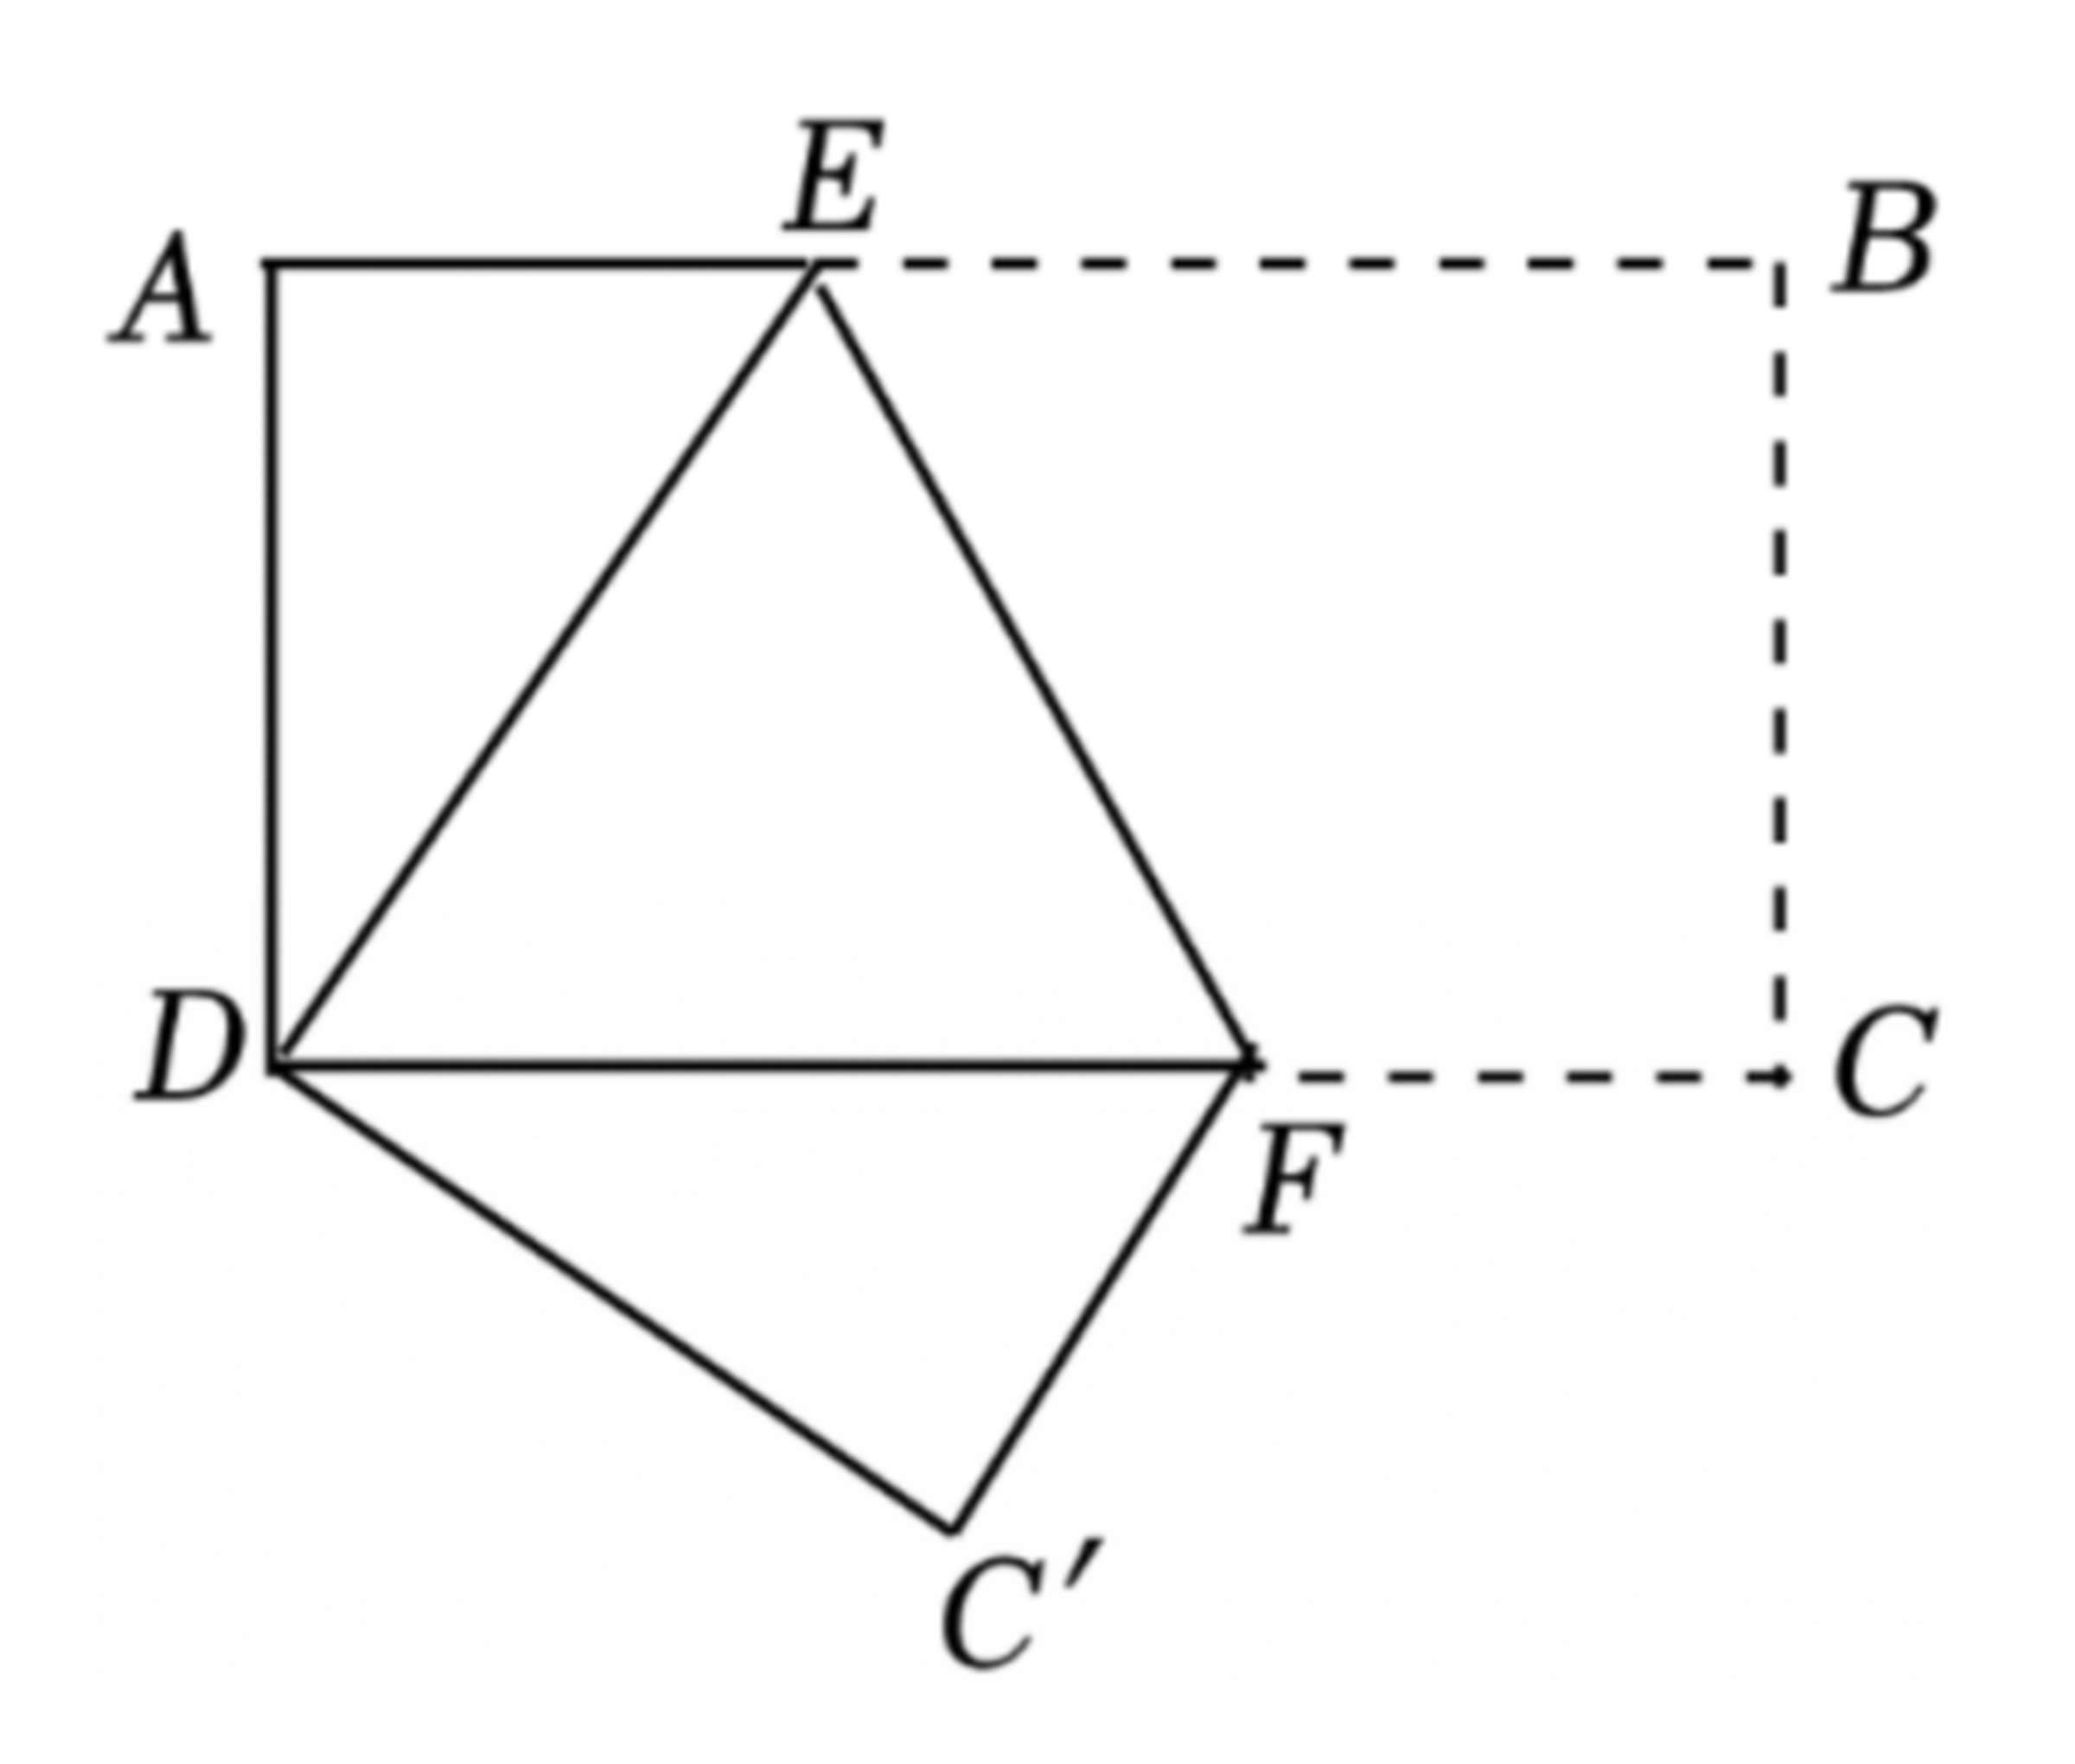
\includegraphics[width=0.40\textwidth]{figures/gao149_q11.png}
\end{center}

\ifanswer
\solbegin
\step{因为矩形 $ABCD(AB>AD)$ 的周长为 12，}
\step{在 $AB$ 和 $CD$ 边上分别取点 $E$ 和 $F$，将四边形 $BCFE$ 沿 $EF$ 折叠，}
\step{使点 $B$ 与点 $D$ 重合，此时点 $C$ 的对应点为 $C'$，}
\step{所以设 $AD=a$，$AB=b$，则 $2(a+b)=12$，}
\step{所以 $a+b=6$，且 $AB>AD$，所以 $b>a>0$，}
\step{设 $DF=x$，则 $C'F=b-x$，在 $Rt\triangle DC'F$ 中，$DC'=BC=a$，}% 几何三角形符号原卷印扁等边细线三角 $\triangle$，照录（放大 02 页确认）；$Rt$ 照录
\step{所以 $a^2+(b-x)^2=x^2$，解得 $x=\dfrac{a^2+b^2}{2b}$，}
\step{因此 $\triangle C'DF$ 的面积 $S=\dfrac{1}{2}\cdot DC'\cdot C'F=\dfrac{1}{2}\cdot a\cdot(b-x)$，}
\step{又 $b-x=b-\dfrac{(6-b)^2+b^2}{2b}=\dfrac{6(b-3)}{b}$，}
\step{所以 $S=\dfrac{1}{2}\cdot a\cdot\dfrac{6(b-3)}{b}=\dfrac{1}{2}\cdot(6-b)\cdot\dfrac{6(b-3)}{b}=\dfrac{3(6-b)(b-3)}{b}$}
\step{$=3\cdot\left(-b-\dfrac{18}{b}+9\right)$，又 $b+\dfrac{18}{b}\geqslant2\sqrt{b\cdot\dfrac{18}{b}}=6\sqrt{2}$，}
\step{当且仅当 $b=\dfrac{18}{b}$ 即 $b=3\sqrt{2}$ 时取等号，此时满足 $b>a$，}
\step{所以 $S\leqslant3\cdot(-6\sqrt{2}+9)=27-18\sqrt{2}$，故 $\triangle C'DF$ 面积的最大值为 $27-18\sqrt{2}$.}
\solend
\fi

% === Q12 === 解析内 3 幅三次函数曲线坐标图（仅答案版出）；解析 15 行（8 行 03 页＋7 行 04 页）
\item 已知 $m>0$，若存在 $t\in\R$，使得对任意 $x\in[0,m]$，不等式 $[(x-1)^2-t](x-t)\leqslant0$ 恒成立，则 $m$ 的最大值是\blankline[4.4em].

\ifanswer
\solbegin
\step{当 $t\leqslant0$ 时，$(x-1)^2-t\geqslant0$ 恒成立，}
\step{不等式 $[(x-1)^2-t](x-t)\leqslant0$ 的解集为 $x\leqslant t$，与 $x\in[0,m]$ 矛盾；}
\step{当 $t>0$ 时，不等式 $[(x-1)^2-t](x-t)\leqslant0\Leftrightarrow(x-1-\sqrt t)(x-1+\sqrt t)(x-t)\leqslant0$，}
\step{若 $t<1-\sqrt t$，即 $t\in\left(0,\dfrac{3-\sqrt5}{2}\right)$，}
\begin{center}
% 情形一 $t<1-\sqrt t$ 曲线图取 03 页右侧，去粉色水印、去色、4× LANCZOS 放大；仅答案版出
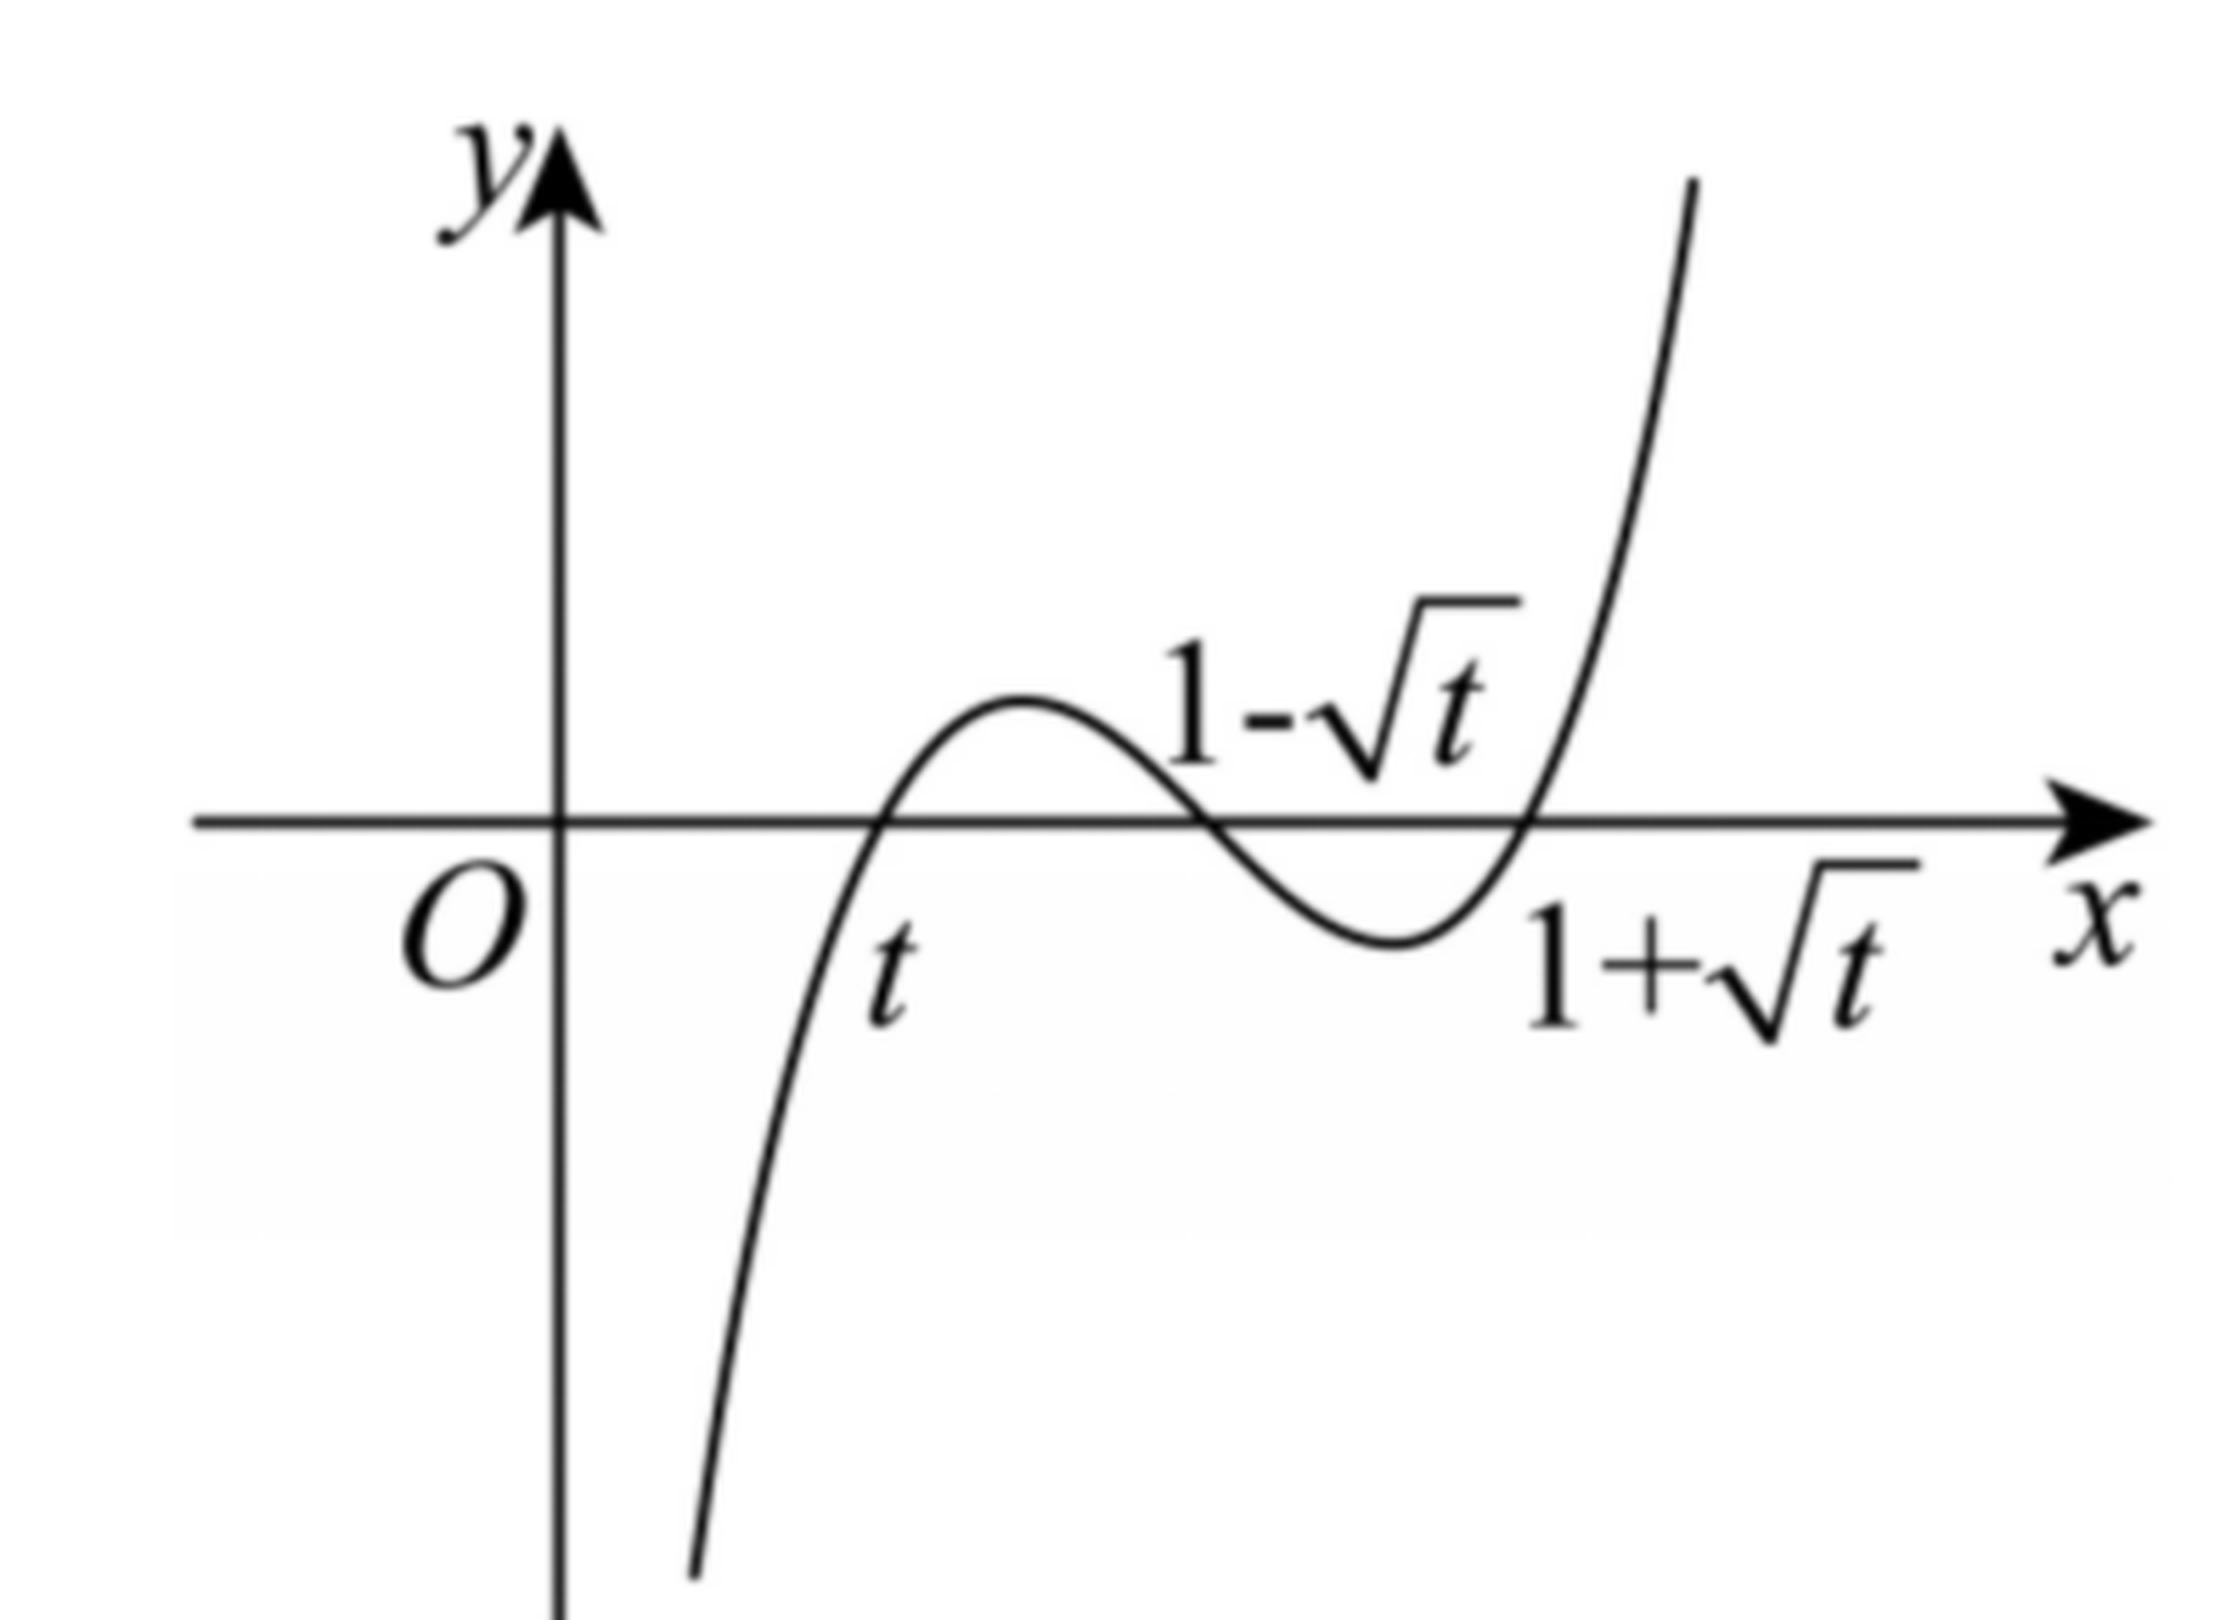
\includegraphics[width=0.40\textwidth]{figures/gao149_q12_a.png}
\end{center}
\step{则原不等式的解集为 $(-\infty,t]\cup[1-\sqrt t,1+\sqrt t]$，}
\step{当 $0<m\leqslant t$ 时，原不等式恒成立，因此}
\step{$m\in\left(0,\dfrac{3-\sqrt5}{2}\right)$；}
\step{若 $t=1-\sqrt t$，即 $t=\dfrac{3-\sqrt5}{2}$，则原不等式的解集为 $(-\infty,1+\sqrt t]$，}
\begin{center}
% 情形二 $t=1-\sqrt t$ 曲线图取 03 页右侧，去粉色水印、去色、4× LANCZOS 放大；仅答案版出
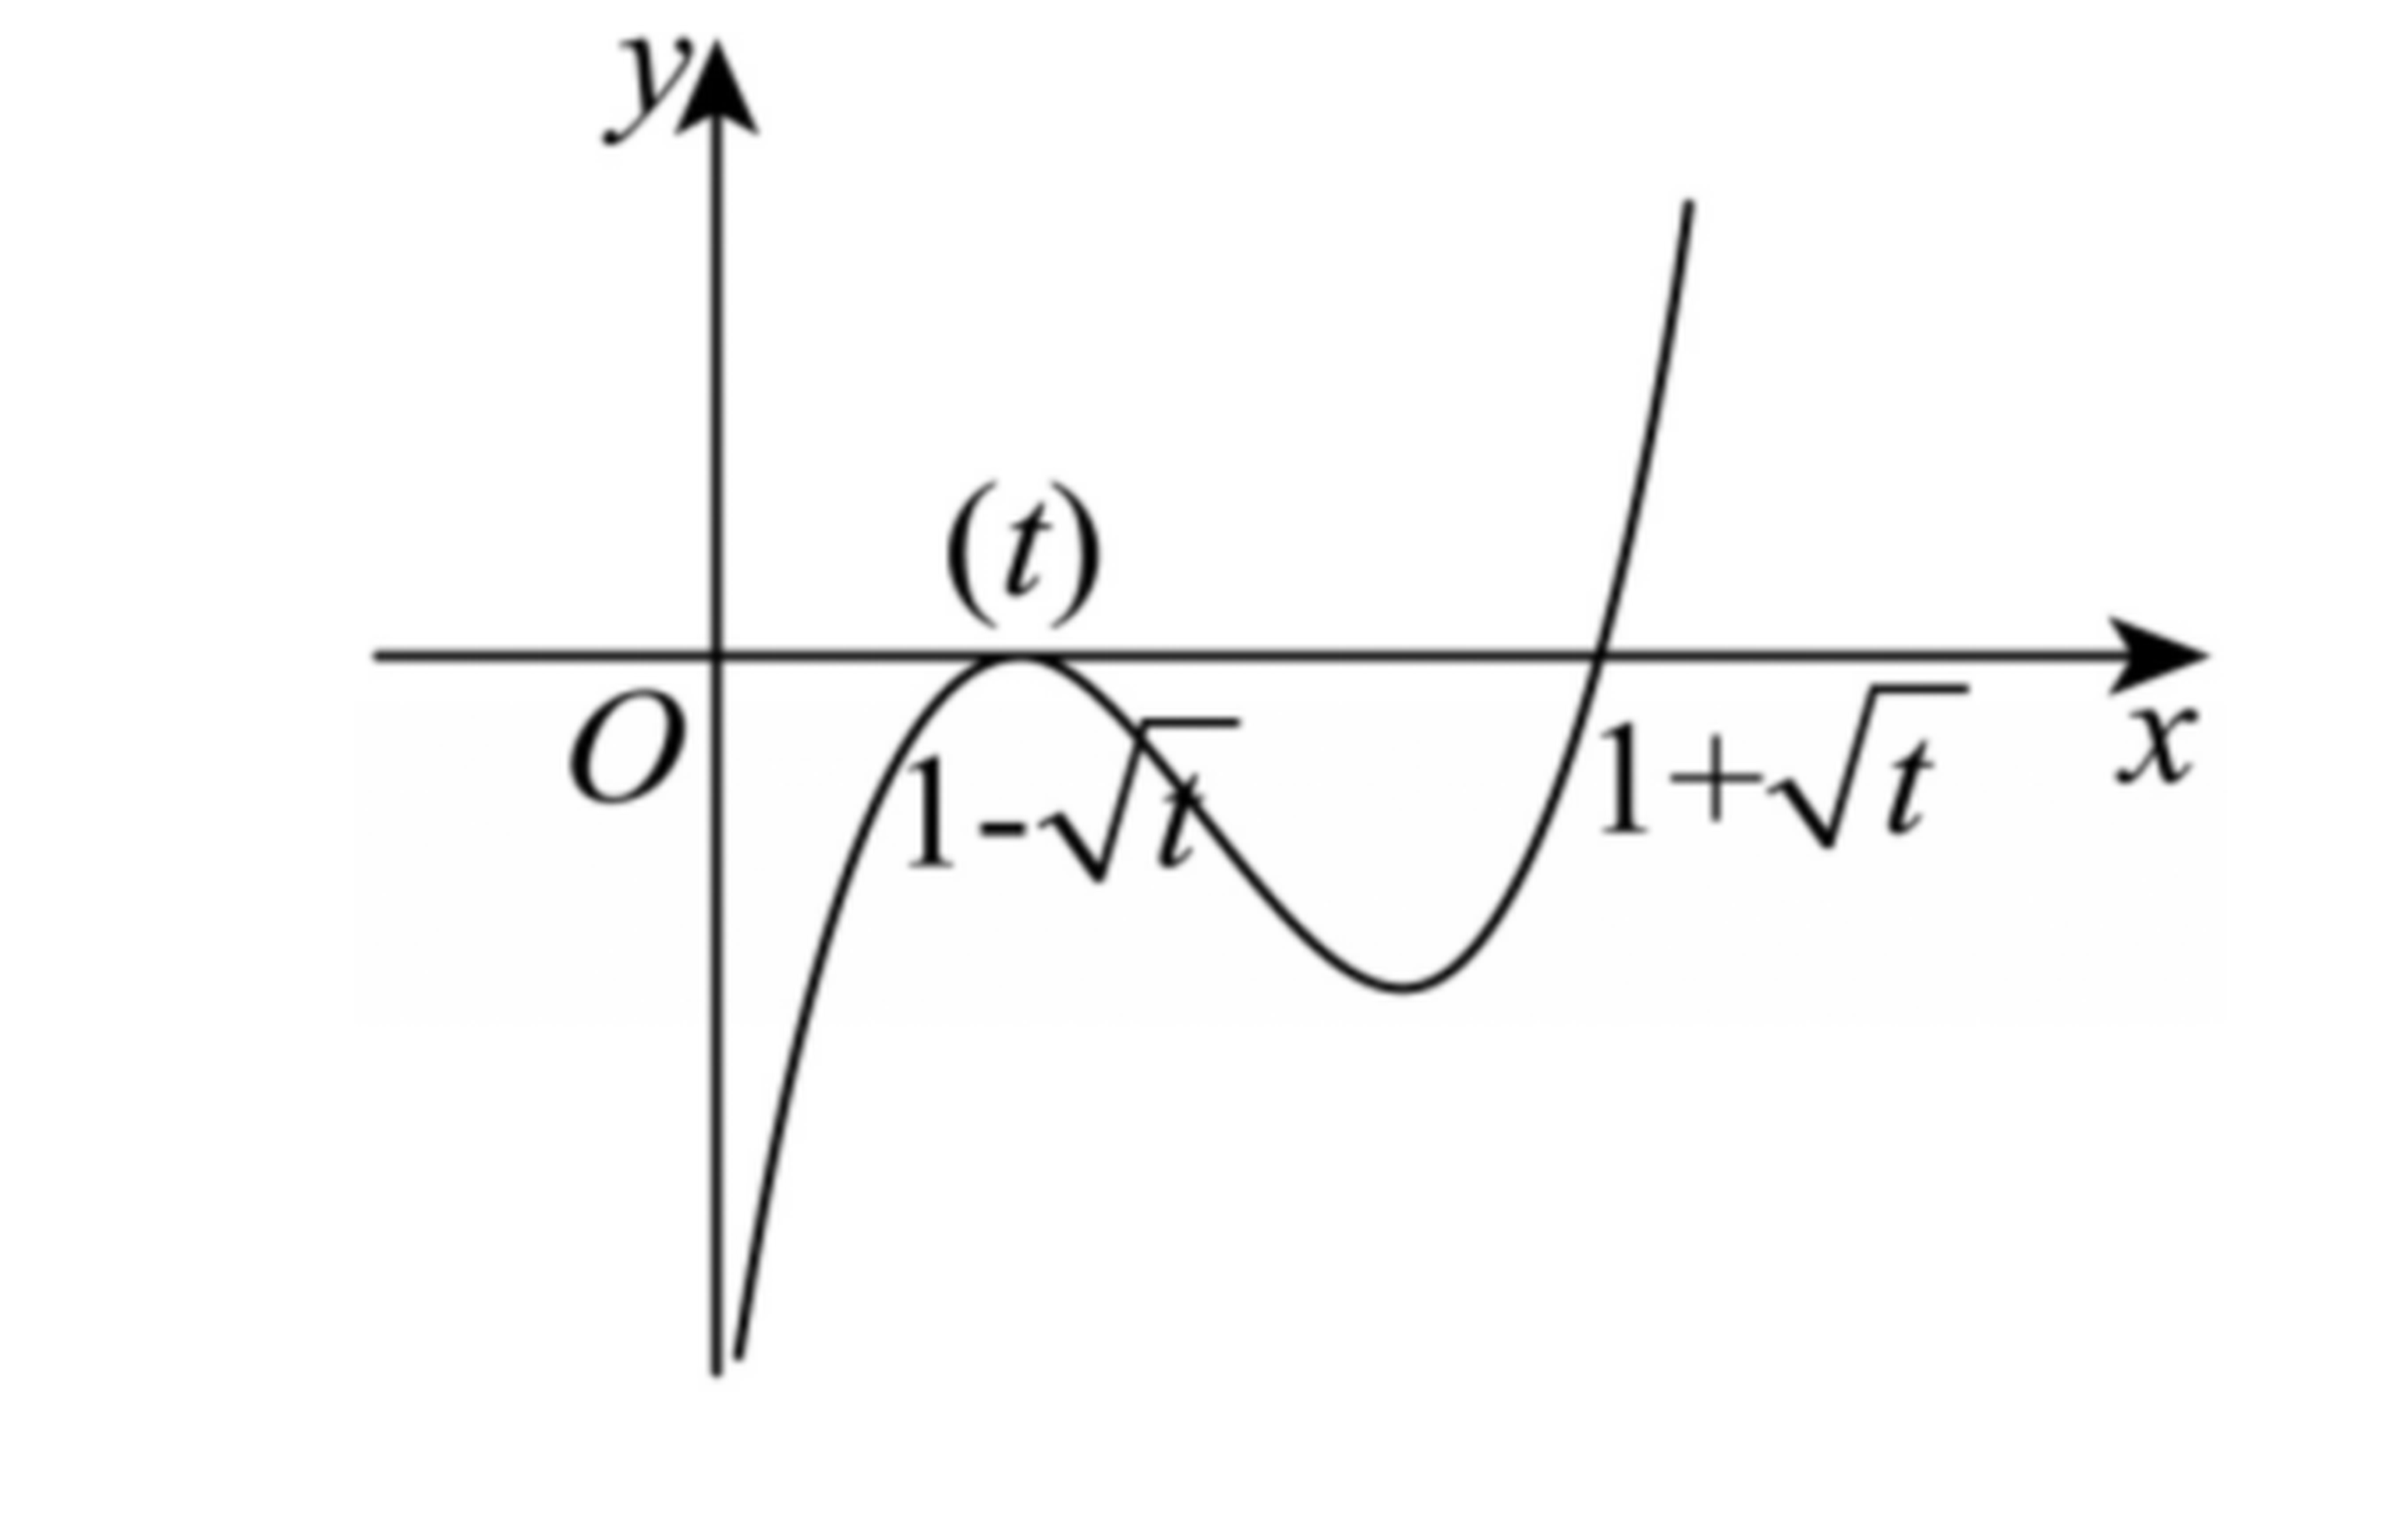
\includegraphics[width=0.40\textwidth]{figures/gao149_q12_b.png}
\end{center}
\step{当 $0<m\leqslant1+\sqrt t$ 时，原不等式恒成立，因此 $m\in\left(0,\dfrac{\sqrt5+1}{2}\right]$；}
\step{若 $1+\sqrt t>t>1-\sqrt t$，即 $t\in\left(\dfrac{3-\sqrt5}{2},\dfrac{3+\sqrt5}{2}\right)$，}
\begin{center}
% 情形三 $1+\sqrt t>t>1-\sqrt t$ 曲线图取 04 页右侧，去粉色水印、去色、4× LANCZOS 放大；仅答案版出
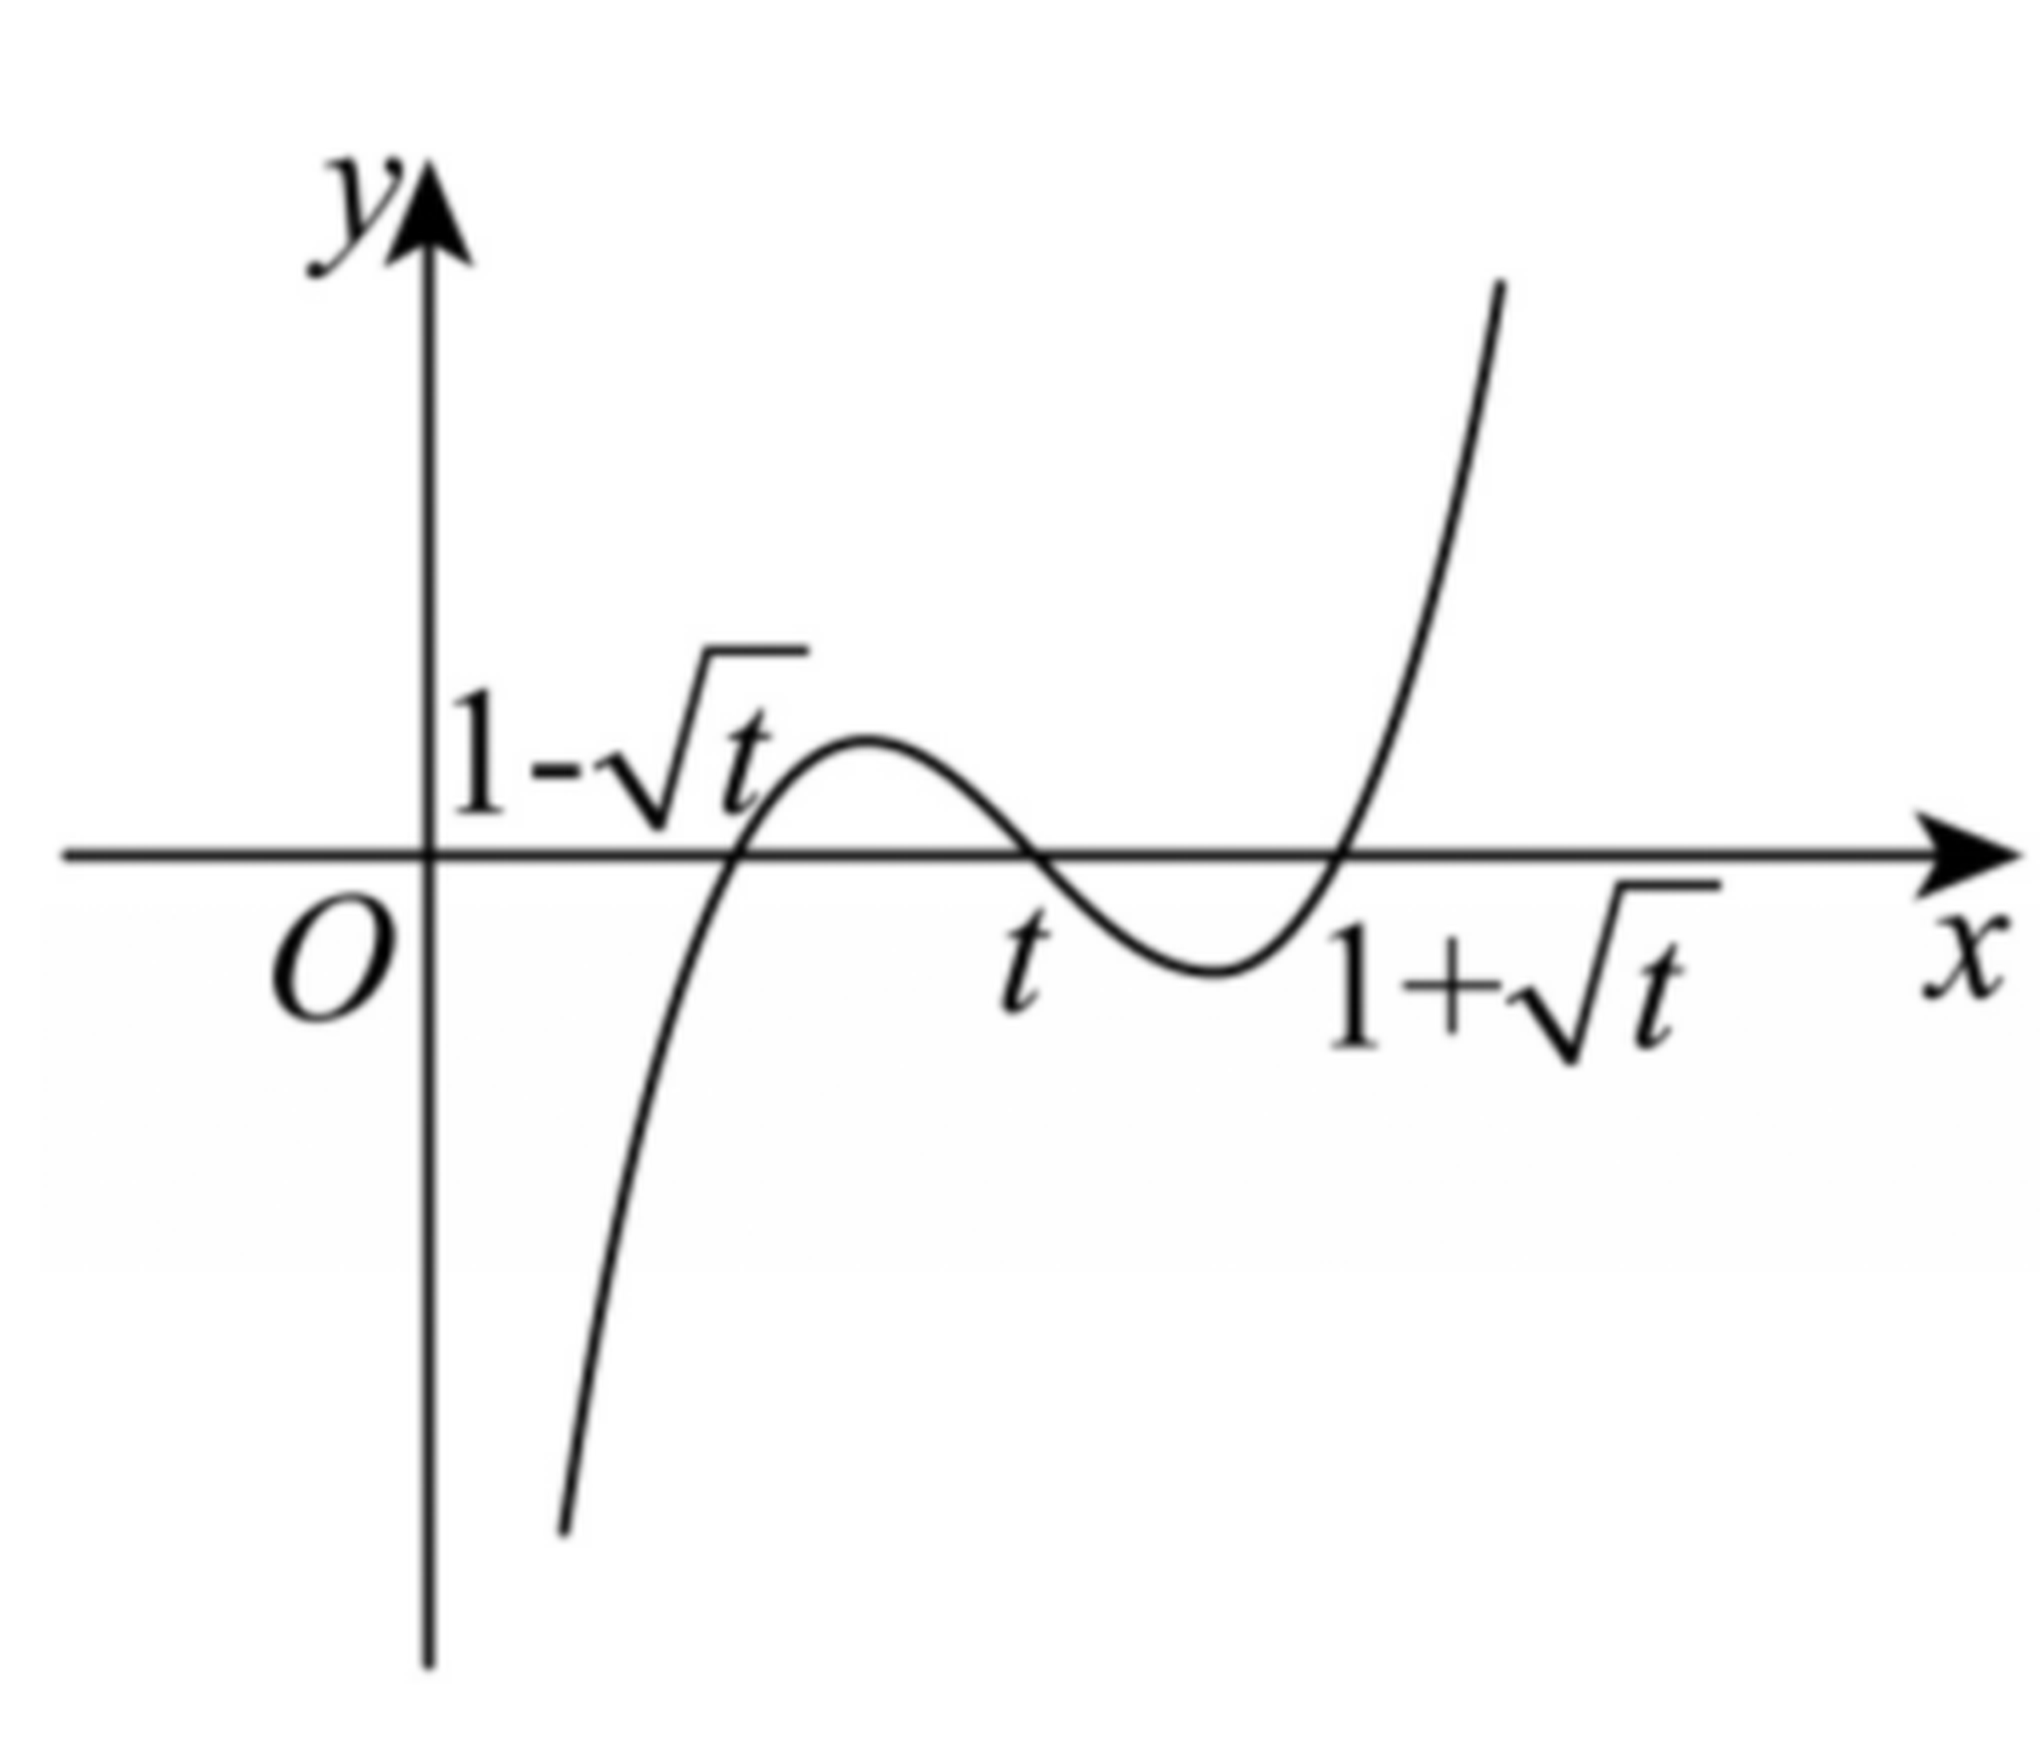
\includegraphics[width=0.40\textwidth]{figures/gao149_q12_c.png}
\end{center}
\step{则原不等式的解集为 $(-\infty,1-\sqrt t]\cup[t,1+\sqrt t]$，}
\step{当 $\begin{cases}1-\sqrt t>0\\1-\sqrt t\geqslant m\end{cases}$ 时，原不等式恒成立，此时 $t\in\left(\dfrac{3-\sqrt5}{2},1\right)$，$m\in\left(0,\dfrac{3-\sqrt5}{2}\right)$；}
\step{若 $t\geqslant1+\sqrt t$，即 $t\geqslant\dfrac{3+\sqrt5}{2}$，则取 $x=0$，$(t-1)t>0$，}
\step{原不等式不恒成立，不符合题意，}
\step{因此实数 $m$ 的取值范围是 $\left(0,\dfrac{\sqrt5+1}{2}\right]$，$m$ 的最大值是 $\dfrac{\sqrt5+1}{2}$.}
\solend
\fi

\end{enumerate}

\bigsec{二、选择题}

\begin{enumerate}
\setcounter{enumi}{12}

% === Q13 ===：答案"C"直接印在题干括号内、无【答案】/【解析】段，按 高一84 Q13／高一148 Q13 成例括号留空、另提 \ans{$C$}；四选项两行两列照原卷分行
\item 设 $ab>0$，则 $a>b$ 是 $\dfrac{1}{a}<\dfrac{1}{b}$ 的\mbox{（\quad）}

\keepwithprev
A. 充分不必要条件\qquad\qquad B. 必要不充分条件

C. 充要条件\qquad\qquad D. 既不充分又不必要条件

\ifanswer
\ans{$C$}
\fi

% === Q14 ===：$A\subset B$ 单线照录；四选项补集照原卷上划线 \overline{A}／\overline{B}；解析 1 行（由韦恩图得 B 对）
\item 已知集合 $A$、$B$ 非空，且 $A\subset B$，则下列式子中一定是空集的为\mbox{（\quad）}

\keepwithprev
A. $\overline{A}\cap B$\qquad B. $A\cap\overline{B}$\qquad C. $\overline{A}\cap\overline{B}$\qquad D. $\overline{A}\cup\overline{B}$

\ifanswer
\solbegin
\step{由韦恩图得 $B$ 对. 故选 $B$.}
\solend
\fi

% === Q15 ===："天文数字"弯引号照录；解析 2 行（首行在 04 页末、末行续 05 页顶）
\item 历史上数学计算方面的三大发明是阿拉伯数字、十进制和对数，其中对数的发明，大大缩短了计算时间，为人类研究科学和了解自然起了重大作用，对数运算对估算“天文数字”具有独特的优势. $2.5^{1000}$ 的估算值约为\mbox{（\quad）}

\keepwithprev
A. $10^{365}$\qquad B. $10^{379}$\qquad C. $10^{389}$\qquad D. $10^{398}$

\ifanswer
\solbegin
\step{$\lg 2.5^{1000}=1000\lg 2.5=1000(1-2\lg 2)\approx1000\times(1-0.602)=398$，}
\step{所以 $2.5^{1000}\approx10^{398}$. 故选 $D$.}
\solend
\fi

% === Q16 ===："完美集"新定义、圈数字①②文本模式；题干"若对任意 $x$，$y\in A$"用全角逗号、解析用顿号"$x$、$y\in A$"，两处照录不统一；解析 9 行
\item 设全集 $U=\R$，集合 $A$ 是一个非空数集，若对任意 $x$，$y\in A$，都有 $x+y\in A$、$xy\in A$，则称集合 $A$ 为一个“完美集”，给出以下命题：

①若 $A_1$、$A_2$ 都是“完美集”，且 $A_1\cap A_2\ne\varnothing$，则 $A_1\cap A_2$ 也是“完美集”；

②若 $A_1$、$A_2$ 都是“完美集”，则 $A_1\cup A_2$ 也是“完美集”.

下列说法正确的是\mbox{（\quad）}

\keepwithprev
A. ①②都是真命题\qquad\qquad B. ①是真命题，②是假命题

C. ①是假命题，②是真命题\qquad\qquad D. ①②都是假命题

\ifanswer
\solbegin
\step{由题意，全集 $U=\R$，集合 $A$ 是一个非空数集，}
\step{若对任意 $x$、$y\in A$，都有 $x+y\in A$、$xy\in A$，则称集合 $A$ 为一个“完美集”，}
\step{对于①，取 $x$、$y\in A_1\cap A_2$，则 $x\in A_1$，$x\in A_2$，$y\in A_1$，$y\in A_2$，}
\step{又 $A_1$、$A_2$ 是“完美集”，所以 $x+y\in A_1$，$xy\in A_1$，$x+y\in A_2$，$xy\in A_2$，}
\step{所以 $x+y\in A_1\cap A_2$，$xy\in A_1\cap A_2$，所以 $A_1\cap A_2$ 是“完美集”，故①正确；}
\step{对于②，取“完美集” $A_1=\{x\mid x=2k,k\in\Z\}$，$A_2=\{x\mid x=3k,k\in\Z\}$，}
\step{则 $2\in A_1$，$3\in A_2$，但 $2+3\notin A_1\cup A_2$，}
\step{即此时 $A_1\cup A_2$ 不是“完美集”，故②错误.}
\step{故选 $B$.}
\solend
\fi
\end{enumerate}

\bigsec{三、解答题}

\begin{enumerate}
\setcounter{enumi}{16}

% === Q17 ===："图像"（有亻）照录（Q17 题干与解析共 2 处）；绝对值 \lvert…\rvert；解析 7 行
\item 已知 $m\in\R$，$f(x)=(m^2-m-5)x^m$. 若 $y=f(x)$ 是幂函数，且其图像不经过原点.

(1) 求实数 $m$ 的值；

(2) 若 $f(a)=f(b)$ 且 $a\ne b$，求 $\lvert a+2\rvert+\lvert b-1\rvert$ 的最小值，并指出取到最小值时 $a$ 的取值范围.

\ifanswer
\solbegin
\step{(1) $f(x)=(m^2-m-5)x^m$ 是幂函数，得 $m^2-m-5=1$，即 $m^2-m-6=0$，}
\step{解得 $m=-2$ 或 $m=3$，又函数图像不经过原点，所以 $m=-2$($3$ 舍)；}
\step{(2) 由 (1) 得 $f(x)=x^{-2}=\dfrac{1}{x^2}$ 为偶函数，}
\step{$x<0$ 时，函数 $f(x)$ 严格增，$x>0$ 时，函数 $f(x)$ 严格减，}
\step{又 $f(a)=f(b)$ 且 $a\ne b$，所以 $a=-b$，且 $a\ne0$，$b\ne0$，}
\step{则 $\lvert a+2\rvert+\lvert b-1\rvert=\lvert a+2\rvert+\lvert-a-1\rvert=\lvert a+2\rvert+\lvert a+1\rvert$，}
\step{则 $\lvert a+2\rvert+\lvert b-1\rvert$ 的最小值为 $1$，取到最小值时 $a$ 的取值范围是 $[-2,-1]$.}
\solend
\fi

% === Q18 ===：判别式两形混用——(1) cases 块印高 \Delta、(2) 独立行印扁 \triangle，逐处照录不统一；解析 8 行
\item 已知命题 $p$：方程 $x^2+4x+m-1=0$ 有两个不等的负根；命题 $q$：方程 $4x^2+4x+m-2=0$ 无实根.

(1) 若 $p$ 为真命题，求 $m$ 的取值范围；

(2) 若 $p$、$q$ 两命题一真一假，求 $m$ 的取值范围.

\ifanswer
\solbegin
\step{(1) 若 $p$ 为真命题，即方程 $x^2+4x+m-1=0$ 有两个不等的负根；}
\step{必有 $\begin{cases}\Delta=16-4(m-1)>0\\m-1>0\end{cases}$，解得 $1<m<5$，即 $m$ 的取值范围为 $(1,5)$；}
\step{(2) 命题 $q$：方程 $4x^2+4x+m-2=0$ 无实根，}
\step{则有 $\triangle=16-16(m-2)<0$，解得 $m>3$，}
\step{若 $p$ 和 $q$ 有且只有一个为真命题，}
\step{若 $p$ 真 $q$ 假，必有 $\begin{cases}1<m<5\\m\leqslant3\end{cases}$，则有 $1<m\leqslant3$，}
\step{若 $p$ 假 $q$ 真，必有 $\begin{cases}m\leqslant1\text{ 或 }m\geqslant5\\m>3\end{cases}$，则有 $m\geqslant5$，}
\step{综上，$1<m\leqslant3$ 或 $m\geqslant5$.}
\solend
\fi

% === Q19 ===：$A\subseteq B$ 带下划线照录；解析 7 行（(2) 两组 cases 并排）
\item 已知 $m\in\R$，集合 $A=\left\{x\mid y=\sqrt{3-x}-\dfrac{1}{\sqrt{x-1}}\right\}$，集合 $B=\{x\mid 2m\leqslant x\leqslant1-m\}$.

(1) 若 $A\cup B=B$，求实数 $m$ 的取值范围；

(2) 若 $A\cap B=\varnothing$，求实数 $m$ 的取值范围.

\ifanswer
\solbegin
\step{(1) 函数 $y=\sqrt{3-x}-\dfrac{1}{\sqrt{x-1}}$，则 $\begin{cases}3-x\geqslant0\\x-1>0\end{cases}$，解得 $1<x\leqslant3$，}
\step{所以 $A=\{x\mid1<x\leqslant3\}$，}
\step{因为 $A\cup B=B$，所以 $A\subseteq B$，则 $\begin{cases}2m\leqslant1\\1-m\geqslant3\end{cases}$，解得 $m\leqslant-2$，}
\step{综上，实数 $m$ 的取值范围为 $(-\infty,-2]$；}
\step{(2) 当 $B=\varnothing$ 时，则 $2m>1-m$，解得 $m>\dfrac{1}{3}$，}
\step{当 $B\ne\varnothing$ 时，则 $\begin{cases}2m\leqslant1-m\\2m>3\end{cases}$ 或 $\begin{cases}2m\leqslant1-m\\1-m\leqslant1\end{cases}$，解得 $m\in\varnothing$ 或 $0\leqslant m\leqslant\dfrac{1}{3}$，}
\step{综上，实数 $m$ 的取值范围为 $[0,+\infty)$.}
\solend
\fi

% === Q20 ===：n 阶基本不等式推广；(3) 解析含 \overbrace{…}^{k} 上括号；(2) 解析"x=x=x=3(1-x)"三连等系原卷笔误、照录加注（见 ⑤）；解析 14 行
\item 教材中的基本不等式可以推广到 $n$ 阶：$n$ 个正数的算术平均数不小于它们的几何平均数，即对于任意的正数 $a_1$、$a_2$、$\cdots$、$a_n$，有 $\dfrac{a_1+a_2+\cdots+a_n}{n}\geqslant\sqrt[n]{a_1\cdot a_2\cdots a_n}$（$n\in\N$ 且 $n\geqslant2$），且等号当且仅当 $a_1=a_2=\cdots=a_n$ 时成立. 利用此结论解决下列问题：

(1) 若 $x$、$y$、$z>0$，求 $\dfrac{y}{x}+\dfrac{2z}{y}+\dfrac{4x}{z}$ 的最小值；

(2) 已知 $0<x<1$，求 $x^3(1-x)$ 的最大值，并求取得最大值时的 $x$ 的值；

(3) 对任意的正整数 $k$，判断 $\left(1+\dfrac{1}{k}\right)^k$ 与 $\left(1+\dfrac{1}{k+1}\right)^{k+1}$ 的大小关系，并证明.

\ifanswer
\solbegin
\step{(1) 因为 $x$、$y$、$z>0$，有 $\dfrac{y}{x}>0$，$\dfrac{2z}{y}>0$，$\dfrac{4x}{z}>0$}
\step{所以 $\dfrac{y}{x}+\dfrac{2z}{y}+\dfrac{4x}{z}\geqslant3\sqrt[3]{\dfrac{y}{x}\cdot\dfrac{2z}{y}\cdot\dfrac{4x}{z}}=3\sqrt[3]{8}=6$，}
\step{当且仅当 $\dfrac{y}{x}=\dfrac{2z}{y}=\dfrac{4x}{z}$ 时取等号，故 $\dfrac{y}{x}+\dfrac{2z}{y}+\dfrac{4x}{z}$ 的最小值为 $6$.}
\step{(2) 因为 $0<x<1$，所以 $1-x>0$，}
\step{$x^3(1-x)=\dfrac{1}{3}[x\cdot x\cdot x\cdot3(1-x)]\leqslant\dfrac{1}{3}\left[\dfrac{x+x+x+3(1-x)}{4}\right]^4=\dfrac{1}{3}\times\left(\dfrac{3}{4}\right)^4$}
\step{$=\dfrac{27}{256}$，当且仅当 $x=x=x=3(1-x)$，即 $x=3(1-x)$，$x=\dfrac{3}{4}$ 取等号，}% 原卷"x=x=x=3(1-x)"三连等，疑为四因子相等之误排，放大 08 页确认，照录未改（见 ⑤）
\step{所以 $0<x<1$ 时，$x^3(1-x)$ 的最大值是 $\dfrac{27}{256}$，取最大值时 $x=\dfrac{3}{4}$.}
\step{(3) 对任意 $k\in\N^*$，$\left(1+\dfrac{1}{k}\right)^k<\left(1+\dfrac{1}{k+1}\right)^{k+1}$.}
\step{证明：$\left(1+\dfrac{1}{k}\right)^k=\overbrace{\left(1+\dfrac{1}{k}\right)\cdot\left(1+\dfrac{1}{k}\right)\cdots\left(1+\dfrac{1}{k}\right)}^{k}\times1$}
\step{$\leqslant\left(\dfrac{\overbrace{\left(1+\dfrac{1}{k}\right)+\left(1+\dfrac{1}{k}\right)+\cdots+\left(1+\dfrac{1}{k}\right)}^{k}+1}{k+1}\right)^{k+1}$}
\step{$=\left(\dfrac{\overbrace{(1+1+\cdots+1)}^{k}+\overbrace{\left(\dfrac{1}{k}+\dfrac{1}{k}+\cdots+\dfrac{1}{k}\right)}^{k}+1}{k+1}\right)^{k+1}=\left(\dfrac{k+1+1}{k+1}\right)^{k+1}=\left(1+\dfrac{1}{k+1}\right)^{k+1}$，}
\step{当且仅当 $1+\dfrac{1}{k}=1$ 时取等号，}
\step{但是任意 $k\in\N^*$ 时 $1+\dfrac{1}{k}>1$，所以等号不成立，}
\step{故任意 $k\in\N^*$ 时，$\left(1+\dfrac{1}{k}\right)^k<\left(1+\dfrac{1}{k+1}\right)^{k+1}$.}
\solend
\fi

% === Q21 ===："减 k 集"新定义（引号内 k／数字两侧空格照录）；解析 26 行（续 10 页），含 ⑤ 三处原卷笔误照录
\item 定义：对于给定的整数 $k$，若非空集合 $A$ 满足如下 3 个条件：

① $A$ 是正整数集的子集；② $A\ne\{1\}$；

③对任意正整数 $x,y$，若 $x+y\in A$，则 $xy-k\in A$；则称集合 $A$ 为“减 $k$ 集”.

(1) 判断集合 $A=\{1,2\}$ 是否为“减 $0$ 集”？是否为“减 $1$ 集”？（无需说明理由）

(2) 证明：不存在“减 $2$ 集”；

(3) 是否存在“减 $1$ 集”？如果存在，求出所有“减 $1$ 集”；如果不存在，说明理由.

\ifanswer
\solbegin
\step{(1) 因为 $P\subseteq\N^*$，$P\ne\{1\}$，$1+1=2\in P$，$1\times1-0\in P$，}
\step{所以集合 $P=\{1,2\}$ 是“减 $0$ 集”；}
\step{因为 $P\subseteq\N^*$，$P\ne\{1\}$，$1+1=2\in P$，$1\times1-1\notin P$，}
\step{所以集合 $P=\{1,2\}$ 是“减 $1$ 集”；}% 按条件③应为"不是"，原卷径印"是"，放大 09 页确认，照录未改（见 ⑤）
\step{(2) 假设存在集合 $A$ 是“减 $2$ 集”，若 $x+y\in A$，则 $xy-2\in A$，}
\step{①当 $x+y=xy-2$ 时，有 $(x-1)(y-1)=3$，}
\step{则 $x$、$y$ 一个为 $2$，一个为 $4$，所以集合 $A$ 有元素 $6$，}
\step{但 $3+3\in A$，$3\times3-2\notin A$，与 $A$ 是“减 $2$ 集”矛盾；}
\step{②当 $x+y\ne xy-2$ 时，则 $x+y=xy-1$ 或 $x+y=xy-m$($m>2$)，}
\step{若 $x+y=xy-1$，$m=1$ 时，$M$ 为除 $1$ 以外的最小元素，}% 原卷"m=1"上文未显式定义，疑笔误，放大 09 页确认，照录未改（见 ⑤）
\step{则 $x=M-1$，$y=1$ 时，$xy-2=M-3$ 小于 $M$，}
\step{要符合题意，必须 $M=4$，}
\step{此时取 $x-2$，$y=2$，$xy-2=2$ 不属于 $A$，故不符合题意，}% 原卷"取 x−2"疑为"取 x=2"误排，放大 09 页确认，照录未改（见 ⑤）
\step{当 $m>2$ 时，$(x-1)(y-1)=m+1$，同样得出矛盾，}
\step{综上，不存在 $A$ 是“减 $2$ 集”.}
\step{(3) 存在“减 $1$ 集” $A$，则 $A\ne\{1\}$，}
\step{①假设 $1\in A$，则 $A$ 中除了元素 $1$ 以外，必然还含有其它元素，}
\step{假设 $2\in A$，$1+1\in A$，而 $1\times1-1\notin A$，所以 $2\notin A$，}
\step{假设 $3\in A$，$1+2\in A$，而 $1\times2-1\in A$，所以 $3\in A$，}
\step{所以 $A=\{1,3\}$，}
\step{假设 $4\in A$，$1+3\in A$，而 $1\times3-1\notin A$，所以 $4\notin A$，}
\step{假设 $5\in A$，$1+4\in A$，$1\times4-1\in A$，$2+3=5$，$2\times3-1\in A$，所以 $5\in A$，}
\step{所以 $A=\{1,3,5\}$，}
\step{以此类推，得 $A=\{1,3,5,\cdots,2n-1,\cdots\}$，($n\in\N^*$)，}
\step{所以所有的“减 $1$ 集”有 $\{1,3\}$，$\{1,3,5\}$，$\{1,3,5,7\}$，$\cdots$，$\{1,3,5,\cdots,2n-1,\cdots\}$，}
\step{$(n\in\N^*)$.}
\solend
\fi
\end{enumerate}

\end{document}
"
% 紧凑版：xelatex "\def\iscompact{1}% 高一149_青浦高级中学上外云间_期中.tex
%   —— 高一上数学"2026-2027 年青浦高级中学上外云间高一上期中"（试卷版/答案版/紧凑版）
% 试卷版：xelatex 高一149_青浦高级中学上外云间_期中.tex
% 答案版：xelatex "\def\isanswer{1}\input{高一149_青浦高级中学上外云间_期中.tex}"
% 紧凑版：xelatex "\def\iscompact{1}\input{高一149_青浦高级中学上外云间_期中.tex}"
%
% ① 原始材料：微信公众号"魔都数学加油站"文章，连载"27学年高一149"，原文标题
% "27学年高一149——2026-2027年上海市青浦高级中学上外云间高一上期中"；
% 原文链接：https://mp.weixin.qq.com/s/T7_nyoR1k0o_5og7FkDsyw 。
% 正文为 10 张 PNG 页（01/02/03/04/10 为 2560×3620，05/06/07/08/09 为 4762×6735，
% 同一篇各页分辨率混排，逐页按各自分辨率裁图核对，别按预览比例换算裁框）。
% 体例：混合体例讲评版——19 题中 Q6 只印【答案】、无【解析】；Q13 的答案"C"
%   直接印在题干括号内、无【答案】/【解析】段；其余 17 题印【解析】（逐题核实，见 ② ②）。
% 题目、答案、解析均据原图转录；卷面粉红色水印"魔都数学加油站"及公众号页脚未录入。
% 全卷插图清单（逐页通读 10 页确认）：1 幅题目配图 + 3 幅【解析】内配图：
%   · Q11 矩形 ABCD 折叠几何图（02 页右侧：A/B/C/D/E/F/C' 与虚线 EB、BC、FC），
%     题干"如图"处，题目配图、三版都出，裁 figures/gao149_q11.png；
%   · Q12【解析】内 3 幅三次函数曲线坐标图（03 页右侧两幅 + 04 页右侧一幅：
%     x/y 轴、O、t、1-\sqrt t、1+\sqrt t 等标注，分别对应 t<1-\sqrt t、
%     t=1-\sqrt t、1+\sqrt t>t>1-\sqrt t 三种情形），解析配图、仅答案版出，
%     分别裁 figures/gao149_q12_a.png／_b.png／_c.png，放 \ifanswer 内 \step 之间
%     （高一73 第 16 题成例）；
%   其余各页逐页确认无其它题目配图、无表格；Q14 解析"由韦恩图得 B 对"仅文字推导、
%   原卷并未印韦恩图；Q9／Q18／Q19 的 cases 块与 Q20(3) 的 \overbrace 为数学块（非图）；
%   10 页下半仅水印、无正文。4 图均取自原卷截图，去粉色水印、去色、4× LANCZOS 放大。
%
% 卷首标题：原卷印作"2026-2027 年青浦高级中学上外云间高一上期中"，年份区间按全稿
% 惯例排 en dash；原卷卷面未印副标题，本稿按同期中卷（高一140／141／143／144／145／
% 146／147／148）知识模块口径补出"集合与常用逻辑用语、不等式、函数"。
%
% 题号体例（逐页核实定稿）：本卷共 19 题——一、填空题 3—12（10 题）、
% 二、选择题 13—16（4 题）、三、解答题 17—21（5 题）。
% 三节分别 \setcounter{enumi}{2}／{12}／{16}。原卷从第 3 题起、无第 1、2 题，
% 本稿保留原题号；全卷无附加题节（Q21 解析末行"（n\in N^*）."为全卷收尾）。
%
% ② 与原卷的排版差异：
%   ① 原文从第 3 题起，本稿保留原题号；共 19 题三节；
%   ② 混合体例逐题核实：Q6（反证法"假设的内容"）只印【答案】、无【解析】，
%      按 高一140 第 5 题／高一145 Q3 成例提 \ans{}、不补造解析；Q13 答案"C"直接
%      印在题干括号内、全卷无该题【答案】/【解析】段，按 高一84 Q13／高一148 Q13
%      成例括号 \mbox{（\quad）} 留空、另提 \ans{$C$}；其余 17 题印【解析】、
%      用 \solbegin…\solend，选择题答案在解析末句"故选 X"（Q14 选 B、Q15 选 D、
%      Q16 选 B，逐个放大 04/05 页核实）、题干括号留空、不另提 \ans{}；
%      答案版【答案】/【解析】标记数 = 19（2 个 \ans ＋ 17 个 \solbegin）
%      = 全卷题数；
%   ③ 原卷卷面未印副标题，本稿按知识模块口径补出；
%   ④ 原卷填空横线按全稿惯例排 \blankline[4.4em]；选择题括号排 \mbox{（\quad）}、
%      选项段前按惯例加 \keepwithprev；Q13／Q16 四选项为两行两列、Q14／Q15
%      选项为一行，照原卷分行；解答题不留作答区、不加 \anspace（原卷为讲评版）；
%   ⑤ 数集：Q6"a,b\in N"、Q8"x\in R"、Q9"a\in R"／"解集为 R"、Q12"t\in R"、
%      Q16"U=R"、Q17"m\in R"、Q19"m\in R"、Q20"n\in N" 原卷印斜体 R/N，
%      按全稿惯例统一改 \R／\N；Q20(3)、Q21 的 $N^*$ 排 \N^*；Q16 解析
%      "$k\in Z$" 排 \Z。绝对值排 \lvert…\rvert（Q17），集合描述竖线排 \mid
%      （Q19、Q16 解析）；不等号按全稿惯例排 \leqslant／\geqslant；
%      补集照原卷上划线排 \overline{A}／\overline{B}（Q14 四选项）；空集
%      \varnothing（Q16、Q19、Q21）；
%   ⑥ 子集符号逐处照录不统一：Q4 题干"{1,2}⊆A⊂{1,2,3,4,5,6}" 前者印带下划线
%      ⊆、照录 \subseteq，后者印单线 ⊂、照录 \subset；Q10"A⊆{-1,1/2,2,3}"、
%      Q19 解析"A⊆B"、Q21 解析"P⊆N*" 均印带下划线 ⊆、照录 \subseteq；
%      Q14"A⊂B" 印单线 ⊂、照录 \subset（逐处放大 01/02/04/07/09 页确认，见 ④）；
%   ⑦ 子题标号 (1)(2)(3) 半角括号照录；圈数字 ①②③ 在文本模式（Q16 两命题、
%      Q21 三个条件与解析的①②）按 common.sty 划入 CJK 字符类渲染；cases 块整体
%      算一个印刷行；\left…\right 不得拆到不同 $…$ 组；数学式内 CJK 用 \text{}
%      （Q18 解析 cases 块"\text{或}"）；Q11 解析"Rt\triangle DC'F" 的 Rt 照录；
%   ⑧ 题干／解析中的中文弯引号按原卷照录：Q6" 已知 a,b\in N，若 ab 能被 5 整除，
%      那么 a、b 中至少有一个能被 5 整除 "（开引号后紧跟"已知"、闭引号后空格接"时"）、
%      Q15"天文数字"、Q16"完美集"、Q21"减 k 集""减 0 集""减 1 集""减 2 集"
%      （引号内 k／数字两侧有空格），注释内一律 ASCII 引号；
%   ⑨ 半角逗号在数学组之间是全稿惯例、非笔误（Q8"$a>0,a\ne1,x\in\R$"、
%      Q21 题干"$x,y$" 等），逐处照录别改；Q16 题干"若对任意 $x$，$y\in A$"
%      用全角逗号而解析用顿号"$x$、$y\in A$"，两处不同均照录；行末西文句点
%      照录为 ASCII `.`；行中全角逗号／顿号照录；
%   ⑩ "图像／图象"逐处放大核：Q10 题干与解析共 6 处均印"图象"（象，无亻）；
%      Q17 题干"其图像不经过原点"与解析"又函数图像不经过原点" 2 处印"图像"
%      （像，有亻），逐处照录未统一改动（放大 02/05/06 页确认）；
%   ⑪ 判别式 Δ/△ 混用是照录项：Q9 解析 cases 块"Δ=4(a−2)²+16(a−2)<0"、
%      Q18(1) cases 块"Δ=16−4(m−1)>0" 两处印等腰偏高粗三角 \Delta；
%      Q18(2) 独立行"△=16−16(m−2)<0" 印扁等边细线三角 \triangle，
%      逐处放大判断、照录不统一（参照 高一142／144／145／146／148 头注④口径）；
%      另 Q11 题干"△C'DF 面积"与解析 3 处"△"（含"Rt△DC'F"）共 4 处几何
%      三角形符号亦印扁细线三角，照录 \triangle（非判别式，字形同类，见 ④）；
%   ⑫ 一条 \step = 原卷解析的一个印刷行，cases 块整体算一个印刷行；别把原卷折行
%      并起来、别把一行拆多条。Q11 十三行（7 行在 02 页＋6 行在 03 页）、
%      Q12 十五行（8 行在 03 页＋7 行在 04 页）、Q16 九行、Q21 二十六行
%      （续 10 页）均按印刷行逐条断，不丢行；
%   ⑬ 配图：Q11 题目配图（三版都出）放 \item 内题干之后 \begin{center}，
%      大图块加 \needvspace{8cm} 守卫把整块推走（守卫放 \item 之前，见
%      高一145 Q14/Q20 成例与切页审计 B 类坑）；Q12 三幅解析配图（仅答案版出）
%      放 \ifanswer 内 \solbegin…\solend 的 \step 之间；三版切页审计均"合计异常：无"；
%   ⑭ 跨页续印按题合并：Q3/4/5 在 01 页；Q6/7/8 题干与解析在 01 页；
%      Q9 题干在 01 页末、解析 4 行在 02 页顶；Q10 题干＋解析在 02 页；
%      Q11 题干＋图＋解析前 7 行在 02 页、解析后 6 行续 03 页顶；
%      Q12 题干＋解析首行在 03 页末、解析续 7 行在 03 页下半＋7 行在 04 页顶，
%      "二、选择题"标题在 04 页下半；Q13/14 题干＋选项＋Q14 解析在 04 页下半；
%      Q15 题干＋选项＋解析首行在 04 页末、末行"所以 2.5^1000≈10^398. 故选 D."
%      续 05 页顶；Q16 题干＋选项＋解析 9 行在 05 页、"三、解答题"标题＋
%      Q17 题干首句在 05 页末；Q17(2)＋解析 7 行、Q18 题干＋解析前 6 行在 06 页；
%      Q18 解析末 2 行续 07 页顶；Q19 题干＋解析 4 行在 07 页上半、
%      解析续 3 行在 07 页下半；Q20 题干(1) 在 07 页末、题干(2)(3)＋解析(1)(2)
%      在 08 页上半、(3) 解析含 \overbrace 的证明在 08 页下半、末行
%      "故任意 k∈N* 时…"续 09 页顶；Q21 题干＋解析(1)(2)(3) 前段在 09 页、
%      解析(3) 后半 9 行续 10 页上半（10 页下半仅水印、无正文）。
%      本稿按题连排，不丢行、不并折行；
%   ⑮ 原卷解析内无红色"法一／法二"之类小标题，故本卷无 \stepm；水印
%      "魔都数学加油站"红色不录入。
%
% ③ 行数复核：一条 \step／\stepm = 原卷解析的一个印刷行，cases 块作一个印刷行计。
%   逐题数（主会话逐页核对定稿）：Q3：1；Q4：2；Q5：2；Q6：0（只印【答案】、
%   提 \ans{}）；Q7：1；Q8：1；Q9：4；Q10：5；Q11：13；Q12：15；
%   Q13：0（答案印在题干括号内、另提 \ans{}）；Q14：1；Q15：2；Q16：9；
%   Q17：7；Q18：8；Q19：7；Q20：14；Q21：26。
%   合计 118 条 \step（本卷无 \stepm：解析内无红色"法一／法二"类小标题），
%   与原卷逐题印刷行相等。全卷 17 题设 \solbegin…\solend ＋ 2 处 \ans{}，
%   答案版【答案】/【解析】标记数 = 19 = 全卷题数。
%
% ④ 判别式／子集符号结论（逐处放大原图照录、不得统一，主会话像素级复核）：
%   判别式全卷 3 处，两形混用逐处照录不统一（参照 高一142／144／145／146／148 头注④）：
%     · Q9 解析 cases 块"Δ=4(a−2)²+16(a−2)<0" 原卷印等腰偏高粗三角（高>宽、
%       粗笔画），照录 \Delta（放大 02 页 /tmp/gao149/z/t02_q9_delta2.png 确认）；
%     · Q18(1) cases 块"Δ=16−4(m−1)>0" 原卷印等腰偏高粗三角（高>宽、粗笔画），
%       照录 \Delta（放大 06 页 /tmp/gao149/z/t06_q18a.png 确认）；
%     · Q18(2) 独立行"△=16−16(m−2)<0" 原卷印扁等边细线三角（宽>高、细线），
%       照录 \triangle（放大 06 页 /tmp/gao149/z/t06_q18b.png 与 Q18(1) 并排确认）。
%   另 Q11 题干"△C'DF"与解析 3 处"△"（含"Rt△DC'F"）共 4 处几何三角形符号
%     亦印扁等边细线三角，照录 \triangle（放大 02 页
%     /tmp/gao149/z/t02_q11_tri2.png 确认），与 Q9／Q18(1) 判别式 \Delta 两形不统一。
%   子集／补集：Q4 题干"{1,2}⊆A⊂{1,2,3,4,5,6}" 前者带下划线 ⊆、照录 \subseteq，
%     后者单线 ⊂、照录 \subset（放大 01 页 /tmp/gao149/z/t01_q3q4.png 确认）；
%     Q10"A⊆{-1,1/2,2,3}"、Q19 解析"A⊆B"、Q21 解析"P⊆N*" 三处带下划线 ⊆、
%     照录 \subseteq；Q14"A⊂B" 单线 ⊂、照录 \subset（放大 04 页
%     /tmp/gao149/z/t04_q14_sub2.png 确认）；Q14 四选项补集 \overline{A}／\overline{B}
%     照原卷上划线；空集 \varnothing（Q16、Q19、Q21）；Q19／Q16 解析集合描述竖线
%     \mid；数集 \R／\N／\N^*／\Z 归一见 ② ⑤。
%
% ⑤ 存疑照录（放大原图确认，照录未改、正文对应处另有 % 注）：
%   1. Q21 解析(1) 第二组"因为 P⊆N*，P≠{1}，1+1=2∈P，1×1−1∉P，所以集合
%      P={1,2} 是"减 1 集"" —— 按条件③（x=y=1 时 xy−1=0 须∈P）应为"不是"，
%      原卷却径印"是"，放大 09 页 /tmp/gao149/z/t09_q21_sol1.png 确认，照录未改
%      （疑为原卷结论笔误）。
%   2. Q21 解析(2)"此时取 x−2，y=2，xy−2=2 不属于 A" —— 按上下文应为
%      "取 x=2"（x−2 疑为 x=2 的误排），放大 09 页
%      /tmp/gao149/z/t09_q21_sol2.png 确认，照录未改。
%   3. Q21 解析(2)"若 x+y=xy−1，m=1 时，M 为除 1 以外的最小元素" 中 $m=1$
%      上文未显式定义 m（仅"x+y=xy−m(m>2)"中出现），放大 09 页确认，照录未改。
%   4. Q20 解析(2)"当且仅当 x=x=x=3(1−x)" 三个 x 连等，疑为原卷排印（应为
%      四个因子 x,x,x,3(1−x) 相等），放大 08 页
%      /tmp/gao149/z/t08_q20_sol2.png 确认，照录未改。
%   5. Q6 只印【答案】、Q13 答案印题干括号内，两题均无【解析】，按成例提
%      \ans{}、未补造解析（见 ② ②）。
%   6. 判别式 Q9／Q18(1) 高 \Delta 与 Q18(2)／Q11 扁 \triangle 两形混用，逐处
%      照录不统一（见 ④）；"图像／图象" Q10 用"图象"、Q17 用"图像"，
%      逐处照录未统一（见 ② ⑩）。
%   全卷除此 6 类外未发现其它笔误／自相矛盾处。
%
% ⑥ 跨页续印按题合并说明：见 ② ⑭。
%
\documentclass[a4paper,11pt]{article}
\usepackage{common}

\begin{document}

\examtitlest[3]{2026--2027 年青浦高级中学上外云间高一上期中}{集合与常用逻辑用语、不等式、函数}

\bigsec{一、填空题}

\begin{enumerate}
\setcounter{enumi}{2}

% === Q3 === 根式化分数指数幂；解析 1 行
\item 根式 $\sqrt{a\sqrt a}$ 化成分数指数幂是\blankline[4.4em].

\ifanswer
\solbegin
\step{$\sqrt{a\sqrt a}=\sqrt{a\cdot a^{\frac{1}{2}}}=\sqrt{a^{1+\frac{1}{2}}}=\sqrt{a^{\frac{3}{2}}}=a^{\frac{3}{2}\times\frac{1}{2}}=a^{\frac{3}{4}}$.}
\solend
\fi

% === Q4 === 题干两种子集符号逐处照录（\subseteq 带下划线／\subset 单线）；解析 2 行
\item 满足 $\{1,2\}\subseteq A\subset\{1,2,3,4,5,6\}$ 的集合 $A$ 共有\blankline[4.4em]个.

\ifanswer
\solbegin
\step{集合 $A$ 满足 $\{1,2\}\subseteq A\subset\{1,2,3,4,5,6\}$，}% 前者带下划线 $\subseteq$、后者单线 $\subset$，逐处照录不统一（放大 01 页确认）
\step{所以集合 $A$ 的个数为集合 $\{3,4,5,6\}$ 的真子集的个数，即为 $2^4-1=15$ 个.}
\solend
\fi

% === Q5 === 解析 2 行
\item 不等式 $\dfrac{2x+1}{x-1}\leqslant0$ 的解集为\blankline[4.4em].

\ifanswer
\solbegin
\step{不等式 $\dfrac{2x+1}{x-1}\leqslant0$ 可化为 $(2x+1)(x-1)\leqslant0$，且 $x-1\ne0$，解得 $-\dfrac{1}{2}\leqslant x<1$，}
\step{即原不等式的解集为 $\left[-\dfrac{1}{2},1\right)$.}
\solend
\fi

% === Q6 === 原卷只印【答案】、无【解析】，按 高一140 第 5 题／高一145 Q3 成例提 \ans{}、不补造解析；弯引号与空格照录
\item 用反证法证明命题 “已知 $a,b\in\N$，若 $ab$ 能被 5 整除，那么 $a$、$b$ 中至少有一个能被 5 整除” 时，假设的内容应该是\blankline[4.4em].

\ifanswer
\ans{$a$、$b$ 都不能被 5 整除}
\fi

% === Q7 === 解析 1 行
\item 若 $\log_3(\log_4 x)=1$，则 $x=$\blankline[4.4em].

\ifanswer
\solbegin
\step{$\log_3(\log_4 x)=1$，则 $\log_4 x=3$，故 $x=64$.}
\solend
\fi

% === Q8 === 半角逗号在数学组之间照录；解析 1 行
\item 已知 $a>0,a\ne1,x\in\R$，且 $a^{2x}=2$，则 $\dfrac{a^{3x}+a^{-3x}}{a^x+a^{-x}}$ 的值为\blankline[4.4em].

\ifanswer
\solbegin
\step{$\dfrac{a^{3x}+a^{-3x}}{a^x+a^{-x}}=a^{2x}-1+a^{-2x}=2-1+\dfrac{1}{2}=\dfrac{3}{2}$.}
\solend
\fi

% === Q9 === 题干在 01 页末、解析 4 行在 02 页顶；cases 块整体算 1 行；判别式高 \Delta
\item 已知 $a\in\R$，若关于 $x$ 的不等式 $(a-2)x^2+2(a-2)x-4<0$ 的解集为 $\R$，则实数 $a$ 的取值范围是\blankline[4.4em].

\ifanswer
\solbegin
\step{当 $a=2$ 时，不等式化为 $-4<0$ 对于任意实数 $x$ 都成立，因此 $a=2$ 满足题意；}
\step{当 $a\ne2$ 时，要使关于 $x$ 的不等式 $(a-2)x^2+2(a-2)x-4<0$ 的解集为 $\R$，}
\step{则 $\begin{cases}a-2<0\\\Delta=4(a-2)^2+16(a-2)<0\end{cases}$，解得 $-2<a<2$.}% cases 块整体算一个印刷行；判别式原卷印等腰偏高粗三角 $\Delta$，照录（放大 02 页确认）
\step{综上，$a$ 的取值范围为 $(-2,2]$.}
\solend
\fi

% === Q10 === "图象"（象，无亻）逐处照录；\subseteq 带下划线；解析 5 行
\item 已知集合 $A=\{\alpha,\beta\}$，且 $A\subseteq\left\{-1,\dfrac{1}{2},2,3\right\}$，函数 $f(x)=x^\alpha$ 与 $g(x)=x^\beta$ 的图象有两个交点，则满足条件的不同集合 $A$ 有\blankline[4.4em]个.

\ifanswer
\solbegin
\step{函数 $y=x^{-1}$ 与 $y=x^{\frac{1}{2}}$，$y=x^2$，$y=x^3$ 的图象分别有 1 个，1 个，2 个交点；}
\step{函数 $y=x^{\frac{1}{2}}$ 与 $y=x^2$，$y=x^3$ 的图象都有 2 个交点；}
\step{函数 $y=x^2$ 与 $y=x^3$ 的图象有 2 个交点，}
\step{函数 $f(x)=x^\alpha$ 与 $g(x)=x^\beta$ 的图象若只有 2 个交点，}
\step{则 $A=\{-1,3\}$ 或 $\left\{\dfrac{1}{2},2\right\}$ 或 $\left\{\dfrac{1}{2},3\right\}$ 或 $\{2,3\}$，有 4 个.}
\solend
\fi

% === Q11 === 题目配图（矩形折叠，三版都出）；\needvspace{8cm} 守卫放 \item 之前；解析 13 行（7 行 02 页＋6 行 03 页）
\needvspace{8cm}
\item 如图，矩形 $ABCD(AB>AD)$ 的周长为 12，在 $AB$ 和 $CD$ 边上分别取点 $E$ 和 $F$，将四边形 $BCFE$ 沿 $EF$ 折叠，使点 $B$ 与点 $D$ 重合，此时点 $C$ 的对应点为 $C'$，则 $\triangle C'DF$ 面积的最大值为\blankline[4.4em].

\begin{center}
% 矩形 ABCD 折叠几何图取 02 页右侧，去粉色水印、去色、4× LANCZOS 放大；三版都出
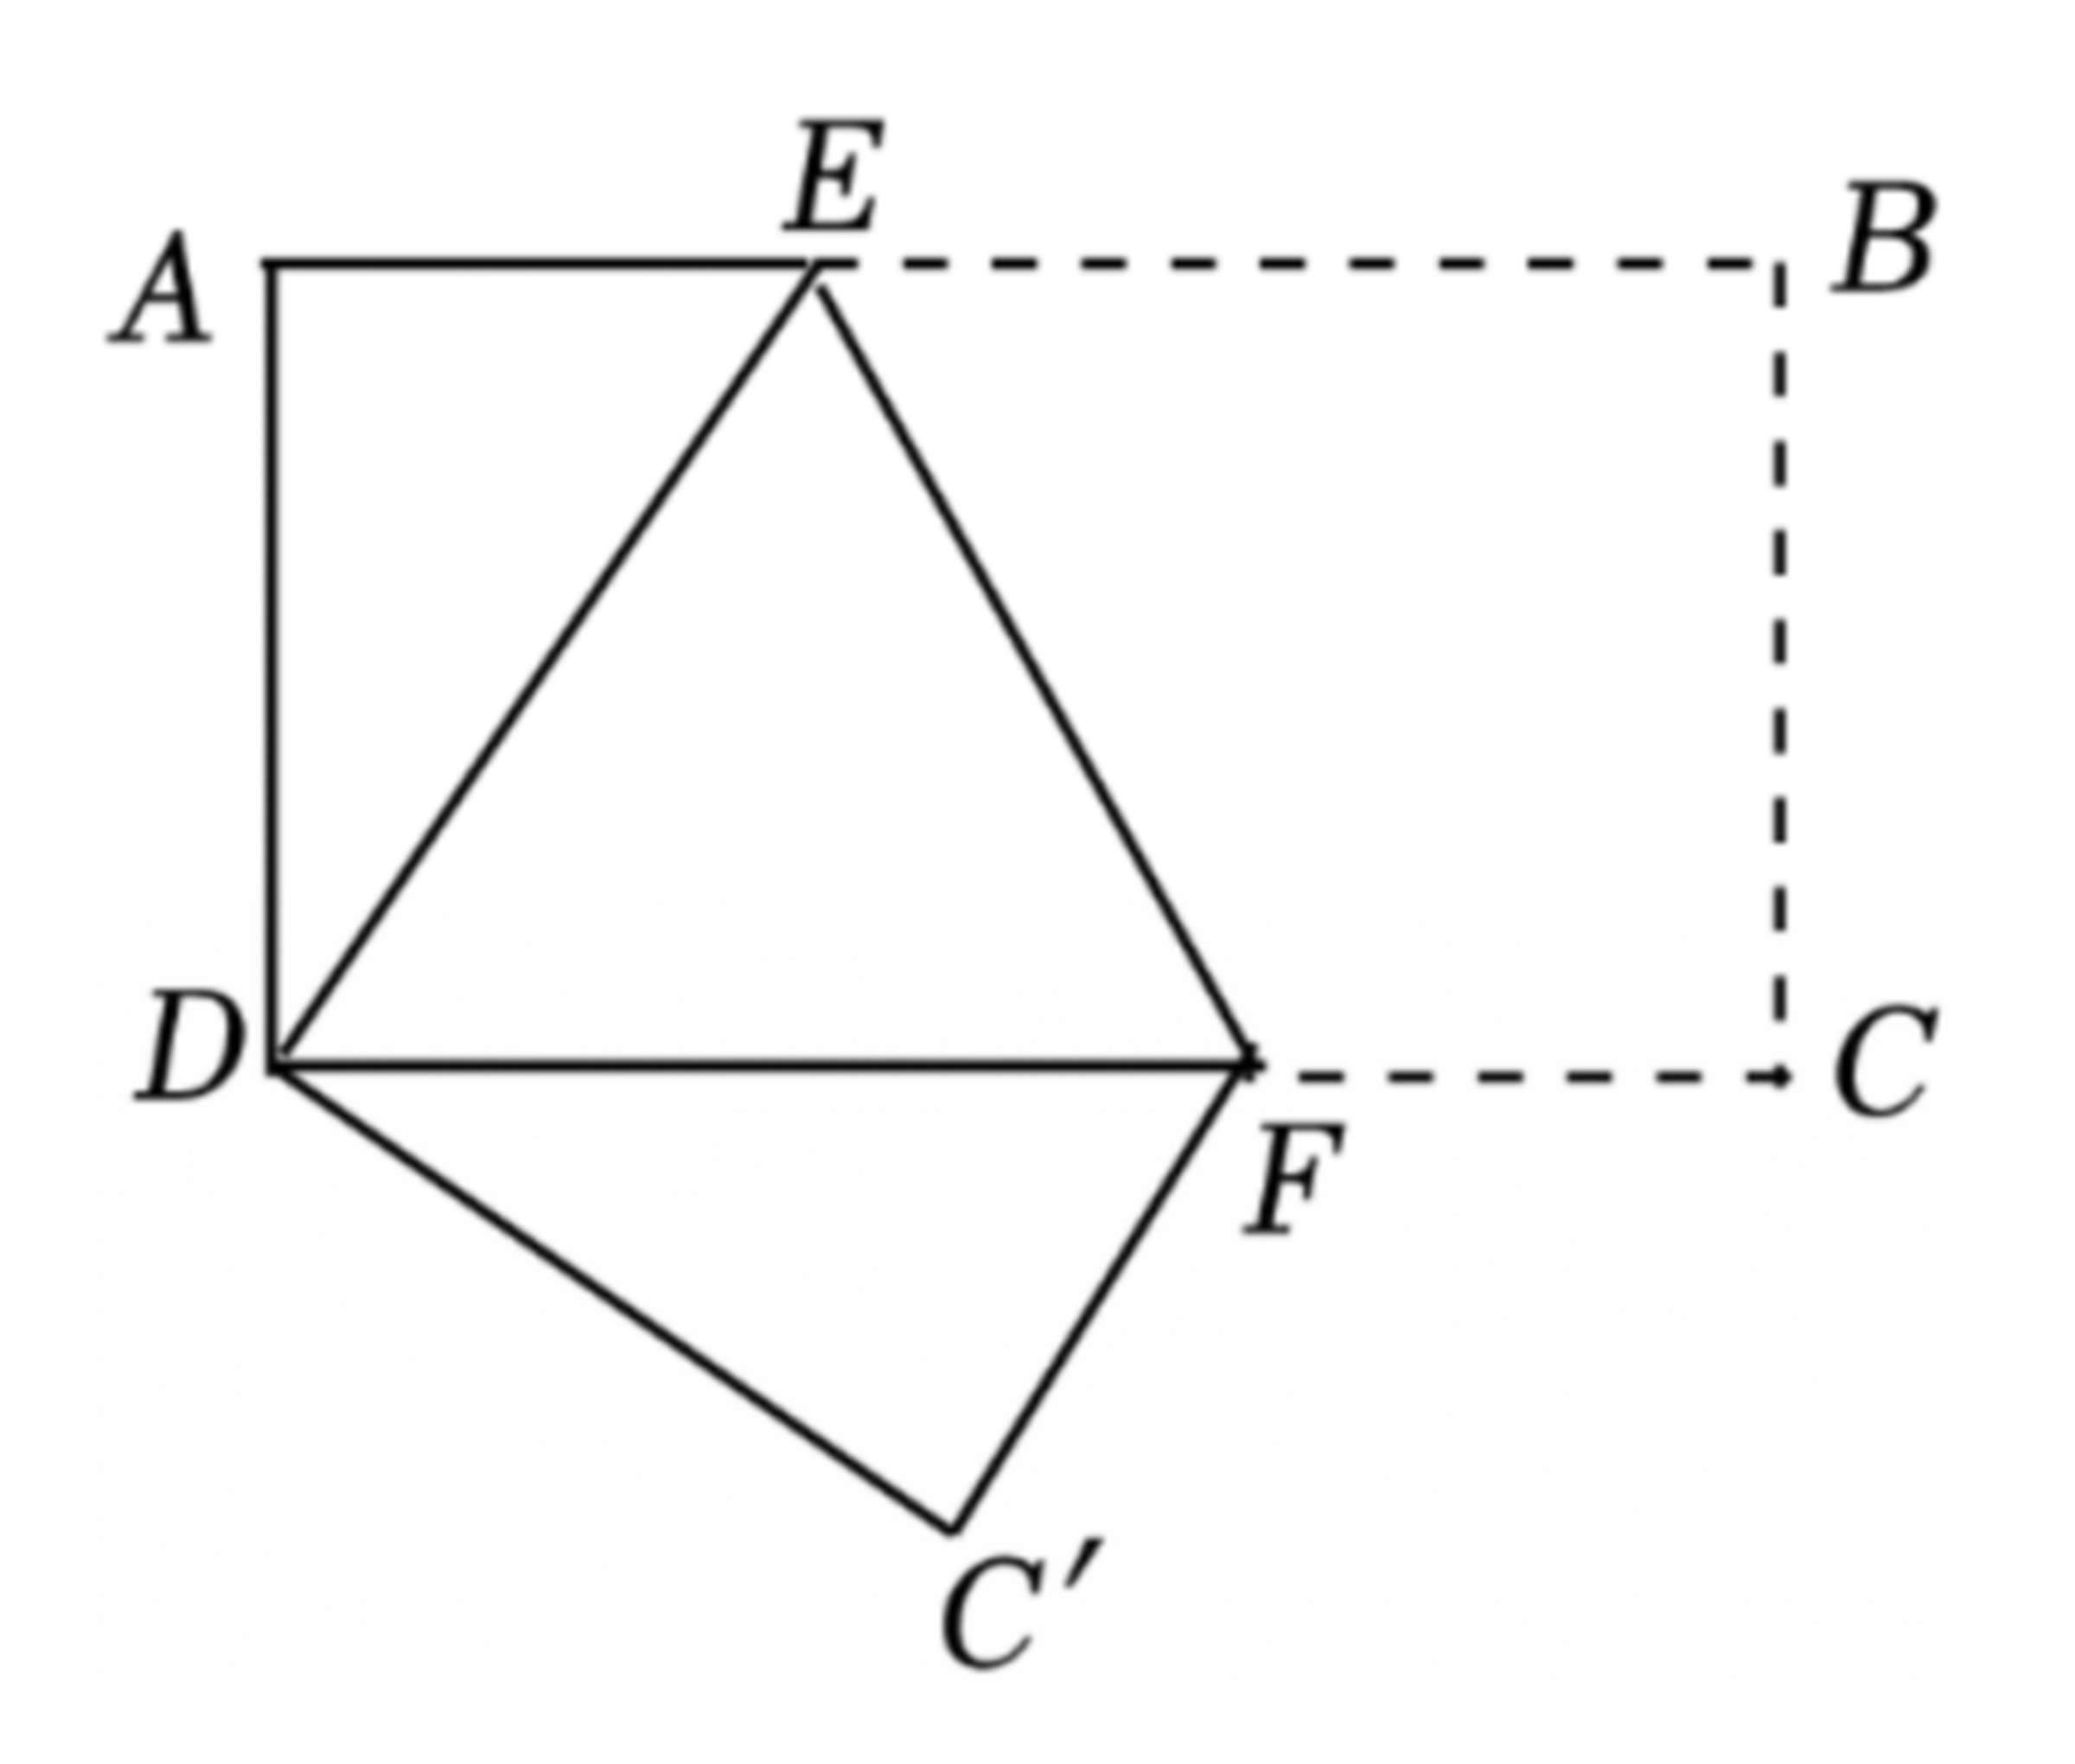
\includegraphics[width=0.40\textwidth]{figures/gao149_q11.png}
\end{center}

\ifanswer
\solbegin
\step{因为矩形 $ABCD(AB>AD)$ 的周长为 12，}
\step{在 $AB$ 和 $CD$ 边上分别取点 $E$ 和 $F$，将四边形 $BCFE$ 沿 $EF$ 折叠，}
\step{使点 $B$ 与点 $D$ 重合，此时点 $C$ 的对应点为 $C'$，}
\step{所以设 $AD=a$，$AB=b$，则 $2(a+b)=12$，}
\step{所以 $a+b=6$，且 $AB>AD$，所以 $b>a>0$，}
\step{设 $DF=x$，则 $C'F=b-x$，在 $Rt\triangle DC'F$ 中，$DC'=BC=a$，}% 几何三角形符号原卷印扁等边细线三角 $\triangle$，照录（放大 02 页确认）；$Rt$ 照录
\step{所以 $a^2+(b-x)^2=x^2$，解得 $x=\dfrac{a^2+b^2}{2b}$，}
\step{因此 $\triangle C'DF$ 的面积 $S=\dfrac{1}{2}\cdot DC'\cdot C'F=\dfrac{1}{2}\cdot a\cdot(b-x)$，}
\step{又 $b-x=b-\dfrac{(6-b)^2+b^2}{2b}=\dfrac{6(b-3)}{b}$，}
\step{所以 $S=\dfrac{1}{2}\cdot a\cdot\dfrac{6(b-3)}{b}=\dfrac{1}{2}\cdot(6-b)\cdot\dfrac{6(b-3)}{b}=\dfrac{3(6-b)(b-3)}{b}$}
\step{$=3\cdot\left(-b-\dfrac{18}{b}+9\right)$，又 $b+\dfrac{18}{b}\geqslant2\sqrt{b\cdot\dfrac{18}{b}}=6\sqrt{2}$，}
\step{当且仅当 $b=\dfrac{18}{b}$ 即 $b=3\sqrt{2}$ 时取等号，此时满足 $b>a$，}
\step{所以 $S\leqslant3\cdot(-6\sqrt{2}+9)=27-18\sqrt{2}$，故 $\triangle C'DF$ 面积的最大值为 $27-18\sqrt{2}$.}
\solend
\fi

% === Q12 === 解析内 3 幅三次函数曲线坐标图（仅答案版出）；解析 15 行（8 行 03 页＋7 行 04 页）
\item 已知 $m>0$，若存在 $t\in\R$，使得对任意 $x\in[0,m]$，不等式 $[(x-1)^2-t](x-t)\leqslant0$ 恒成立，则 $m$ 的最大值是\blankline[4.4em].

\ifanswer
\solbegin
\step{当 $t\leqslant0$ 时，$(x-1)^2-t\geqslant0$ 恒成立，}
\step{不等式 $[(x-1)^2-t](x-t)\leqslant0$ 的解集为 $x\leqslant t$，与 $x\in[0,m]$ 矛盾；}
\step{当 $t>0$ 时，不等式 $[(x-1)^2-t](x-t)\leqslant0\Leftrightarrow(x-1-\sqrt t)(x-1+\sqrt t)(x-t)\leqslant0$，}
\step{若 $t<1-\sqrt t$，即 $t\in\left(0,\dfrac{3-\sqrt5}{2}\right)$，}
\begin{center}
% 情形一 $t<1-\sqrt t$ 曲线图取 03 页右侧，去粉色水印、去色、4× LANCZOS 放大；仅答案版出
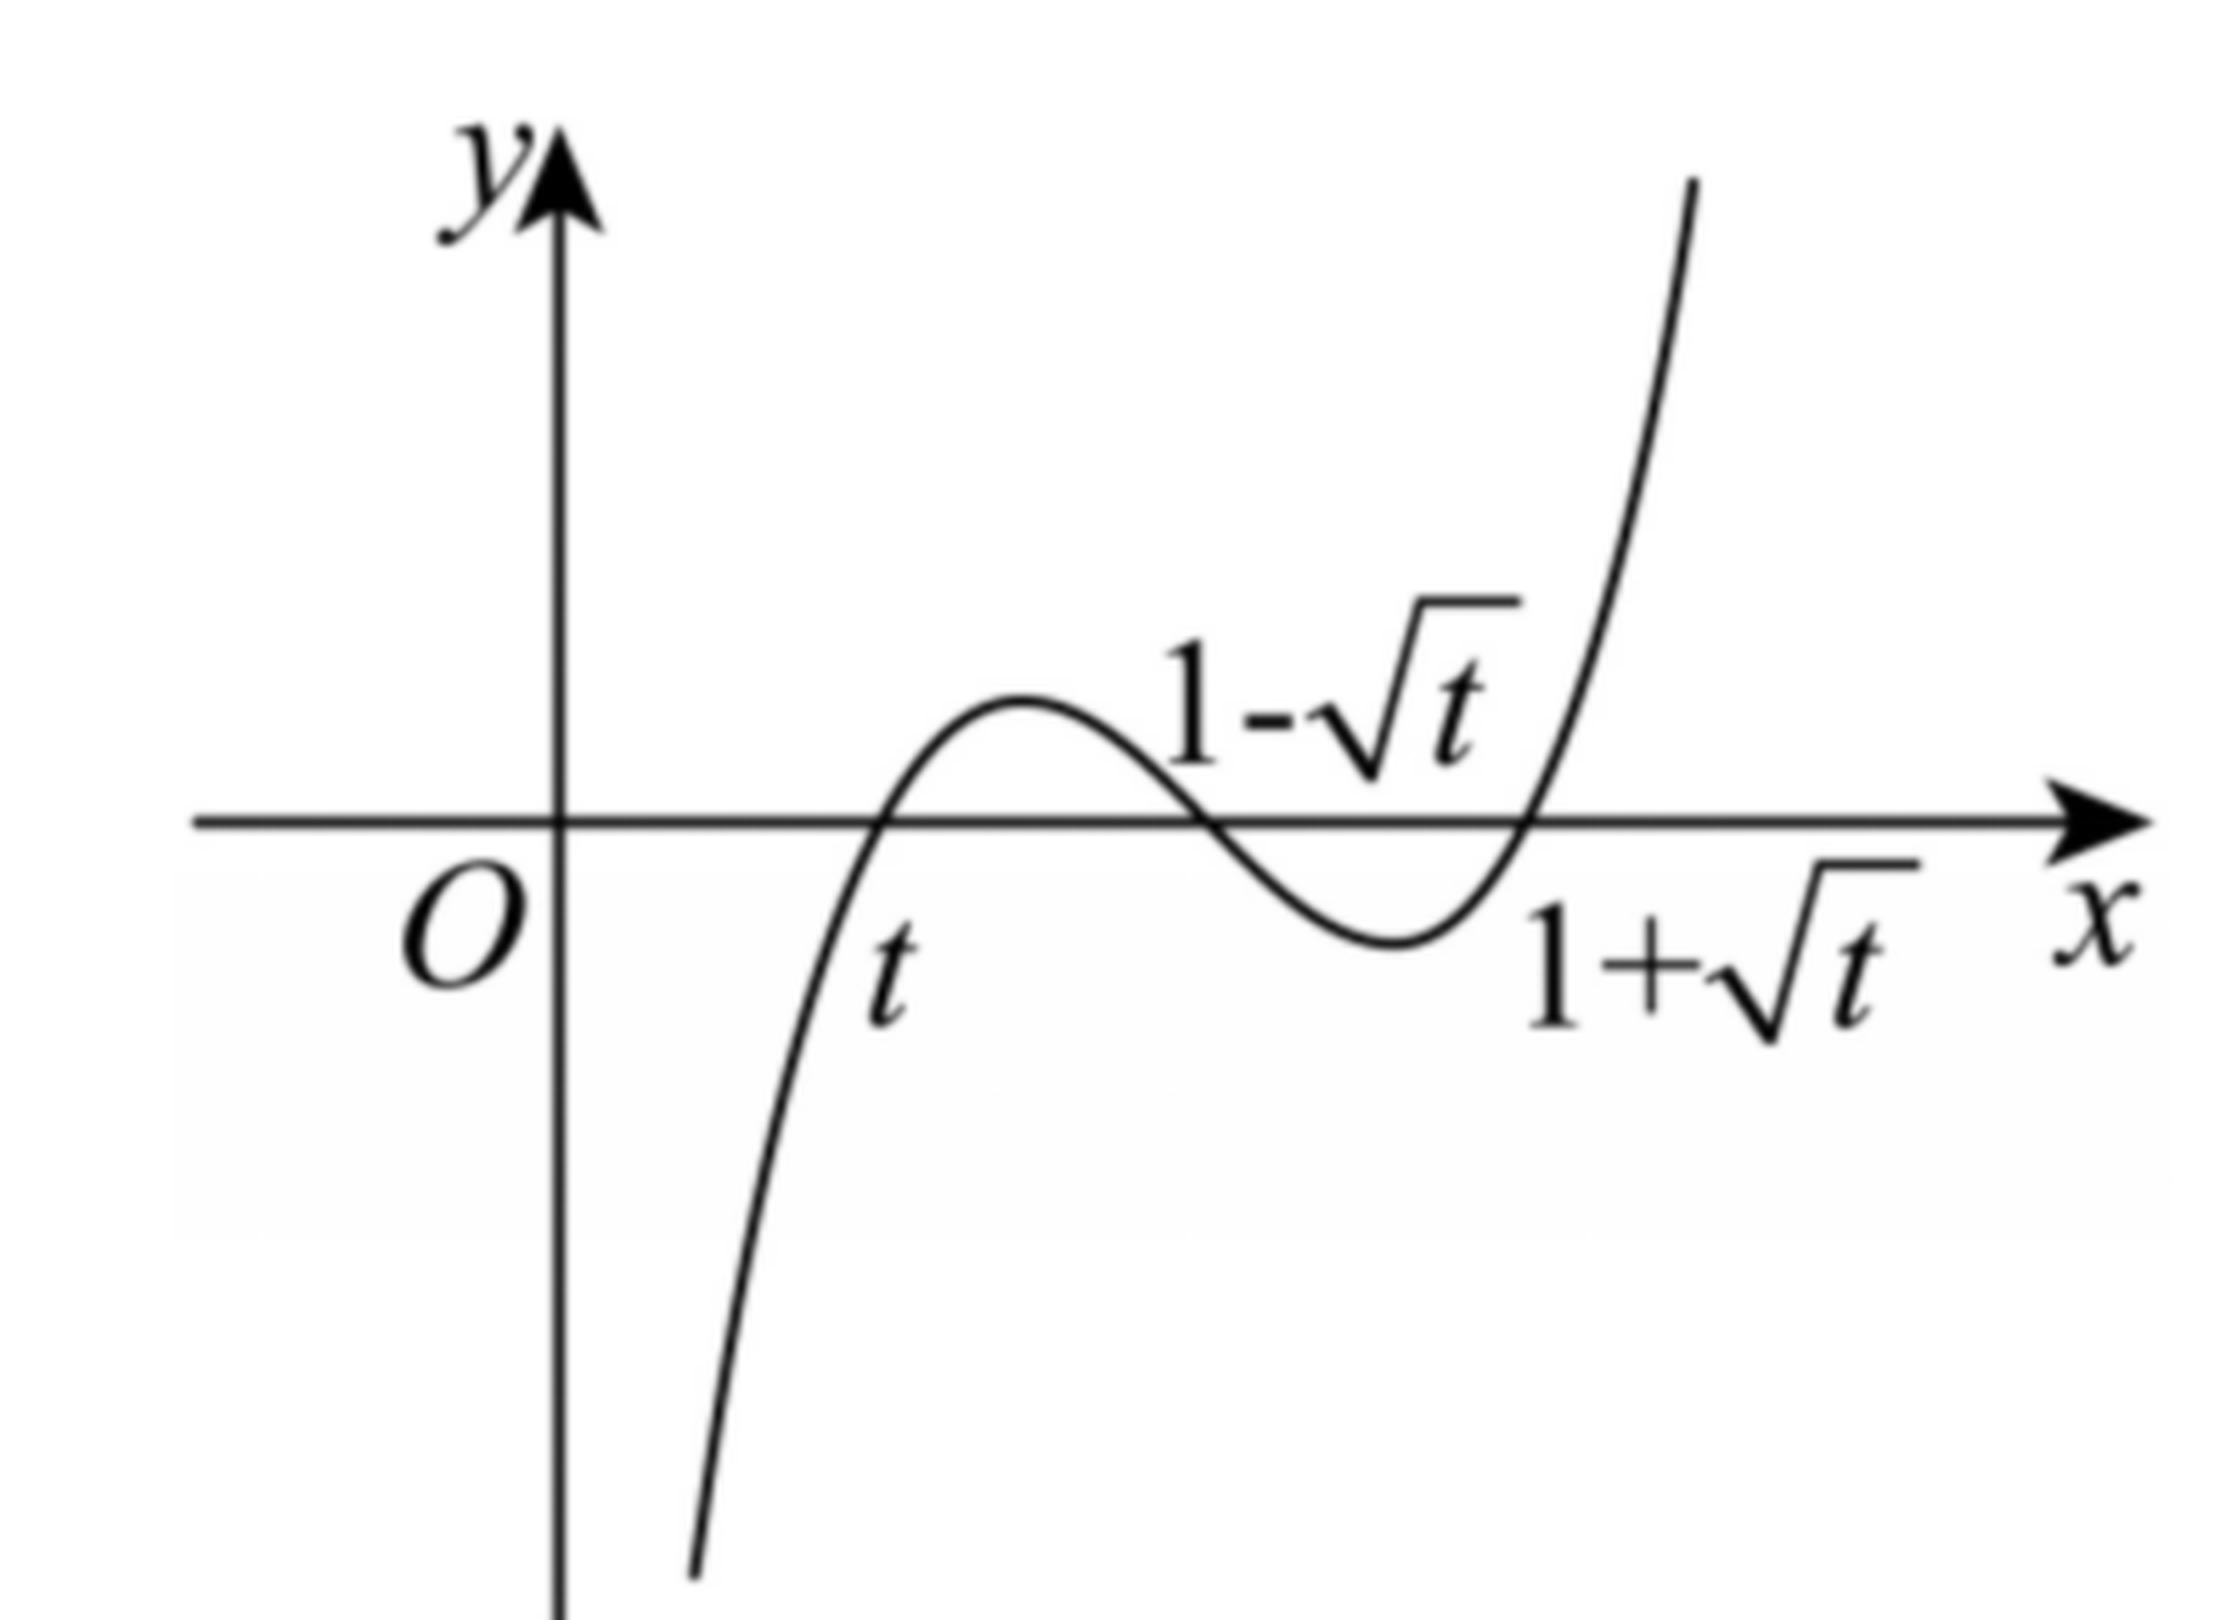
\includegraphics[width=0.40\textwidth]{figures/gao149_q12_a.png}
\end{center}
\step{则原不等式的解集为 $(-\infty,t]\cup[1-\sqrt t,1+\sqrt t]$，}
\step{当 $0<m\leqslant t$ 时，原不等式恒成立，因此}
\step{$m\in\left(0,\dfrac{3-\sqrt5}{2}\right)$；}
\step{若 $t=1-\sqrt t$，即 $t=\dfrac{3-\sqrt5}{2}$，则原不等式的解集为 $(-\infty,1+\sqrt t]$，}
\begin{center}
% 情形二 $t=1-\sqrt t$ 曲线图取 03 页右侧，去粉色水印、去色、4× LANCZOS 放大；仅答案版出
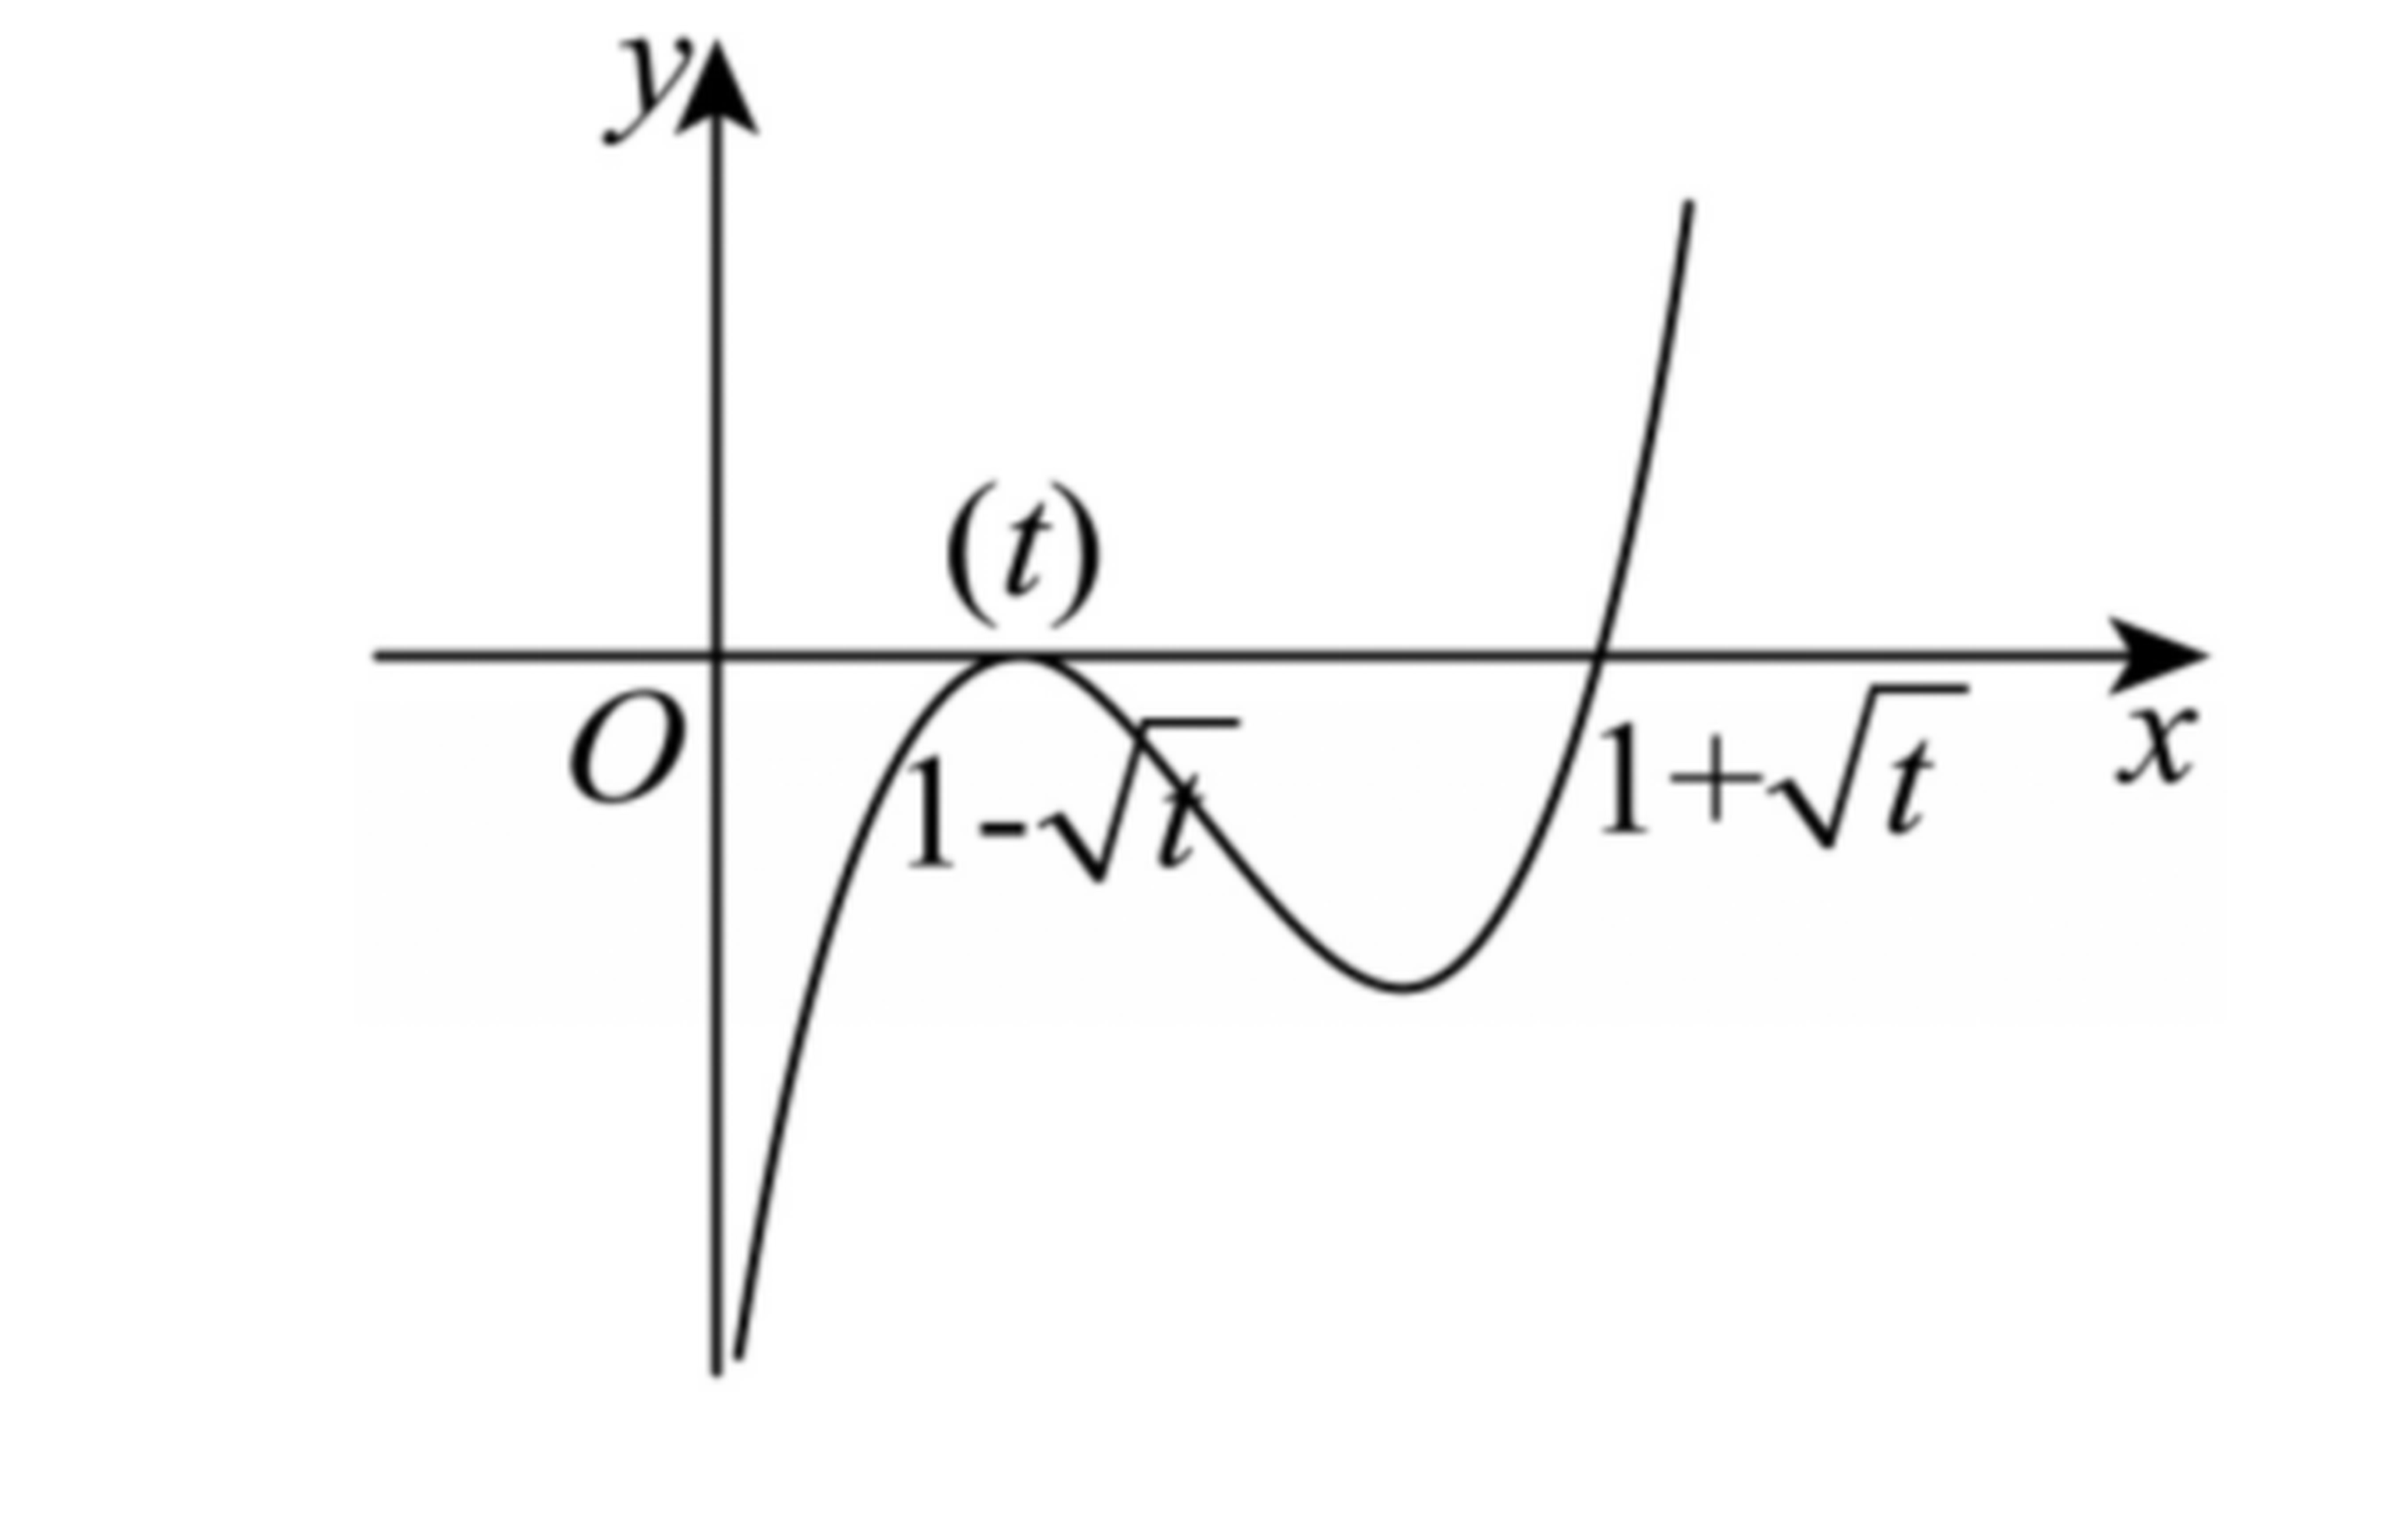
\includegraphics[width=0.40\textwidth]{figures/gao149_q12_b.png}
\end{center}
\step{当 $0<m\leqslant1+\sqrt t$ 时，原不等式恒成立，因此 $m\in\left(0,\dfrac{\sqrt5+1}{2}\right]$；}
\step{若 $1+\sqrt t>t>1-\sqrt t$，即 $t\in\left(\dfrac{3-\sqrt5}{2},\dfrac{3+\sqrt5}{2}\right)$，}
\begin{center}
% 情形三 $1+\sqrt t>t>1-\sqrt t$ 曲线图取 04 页右侧，去粉色水印、去色、4× LANCZOS 放大；仅答案版出
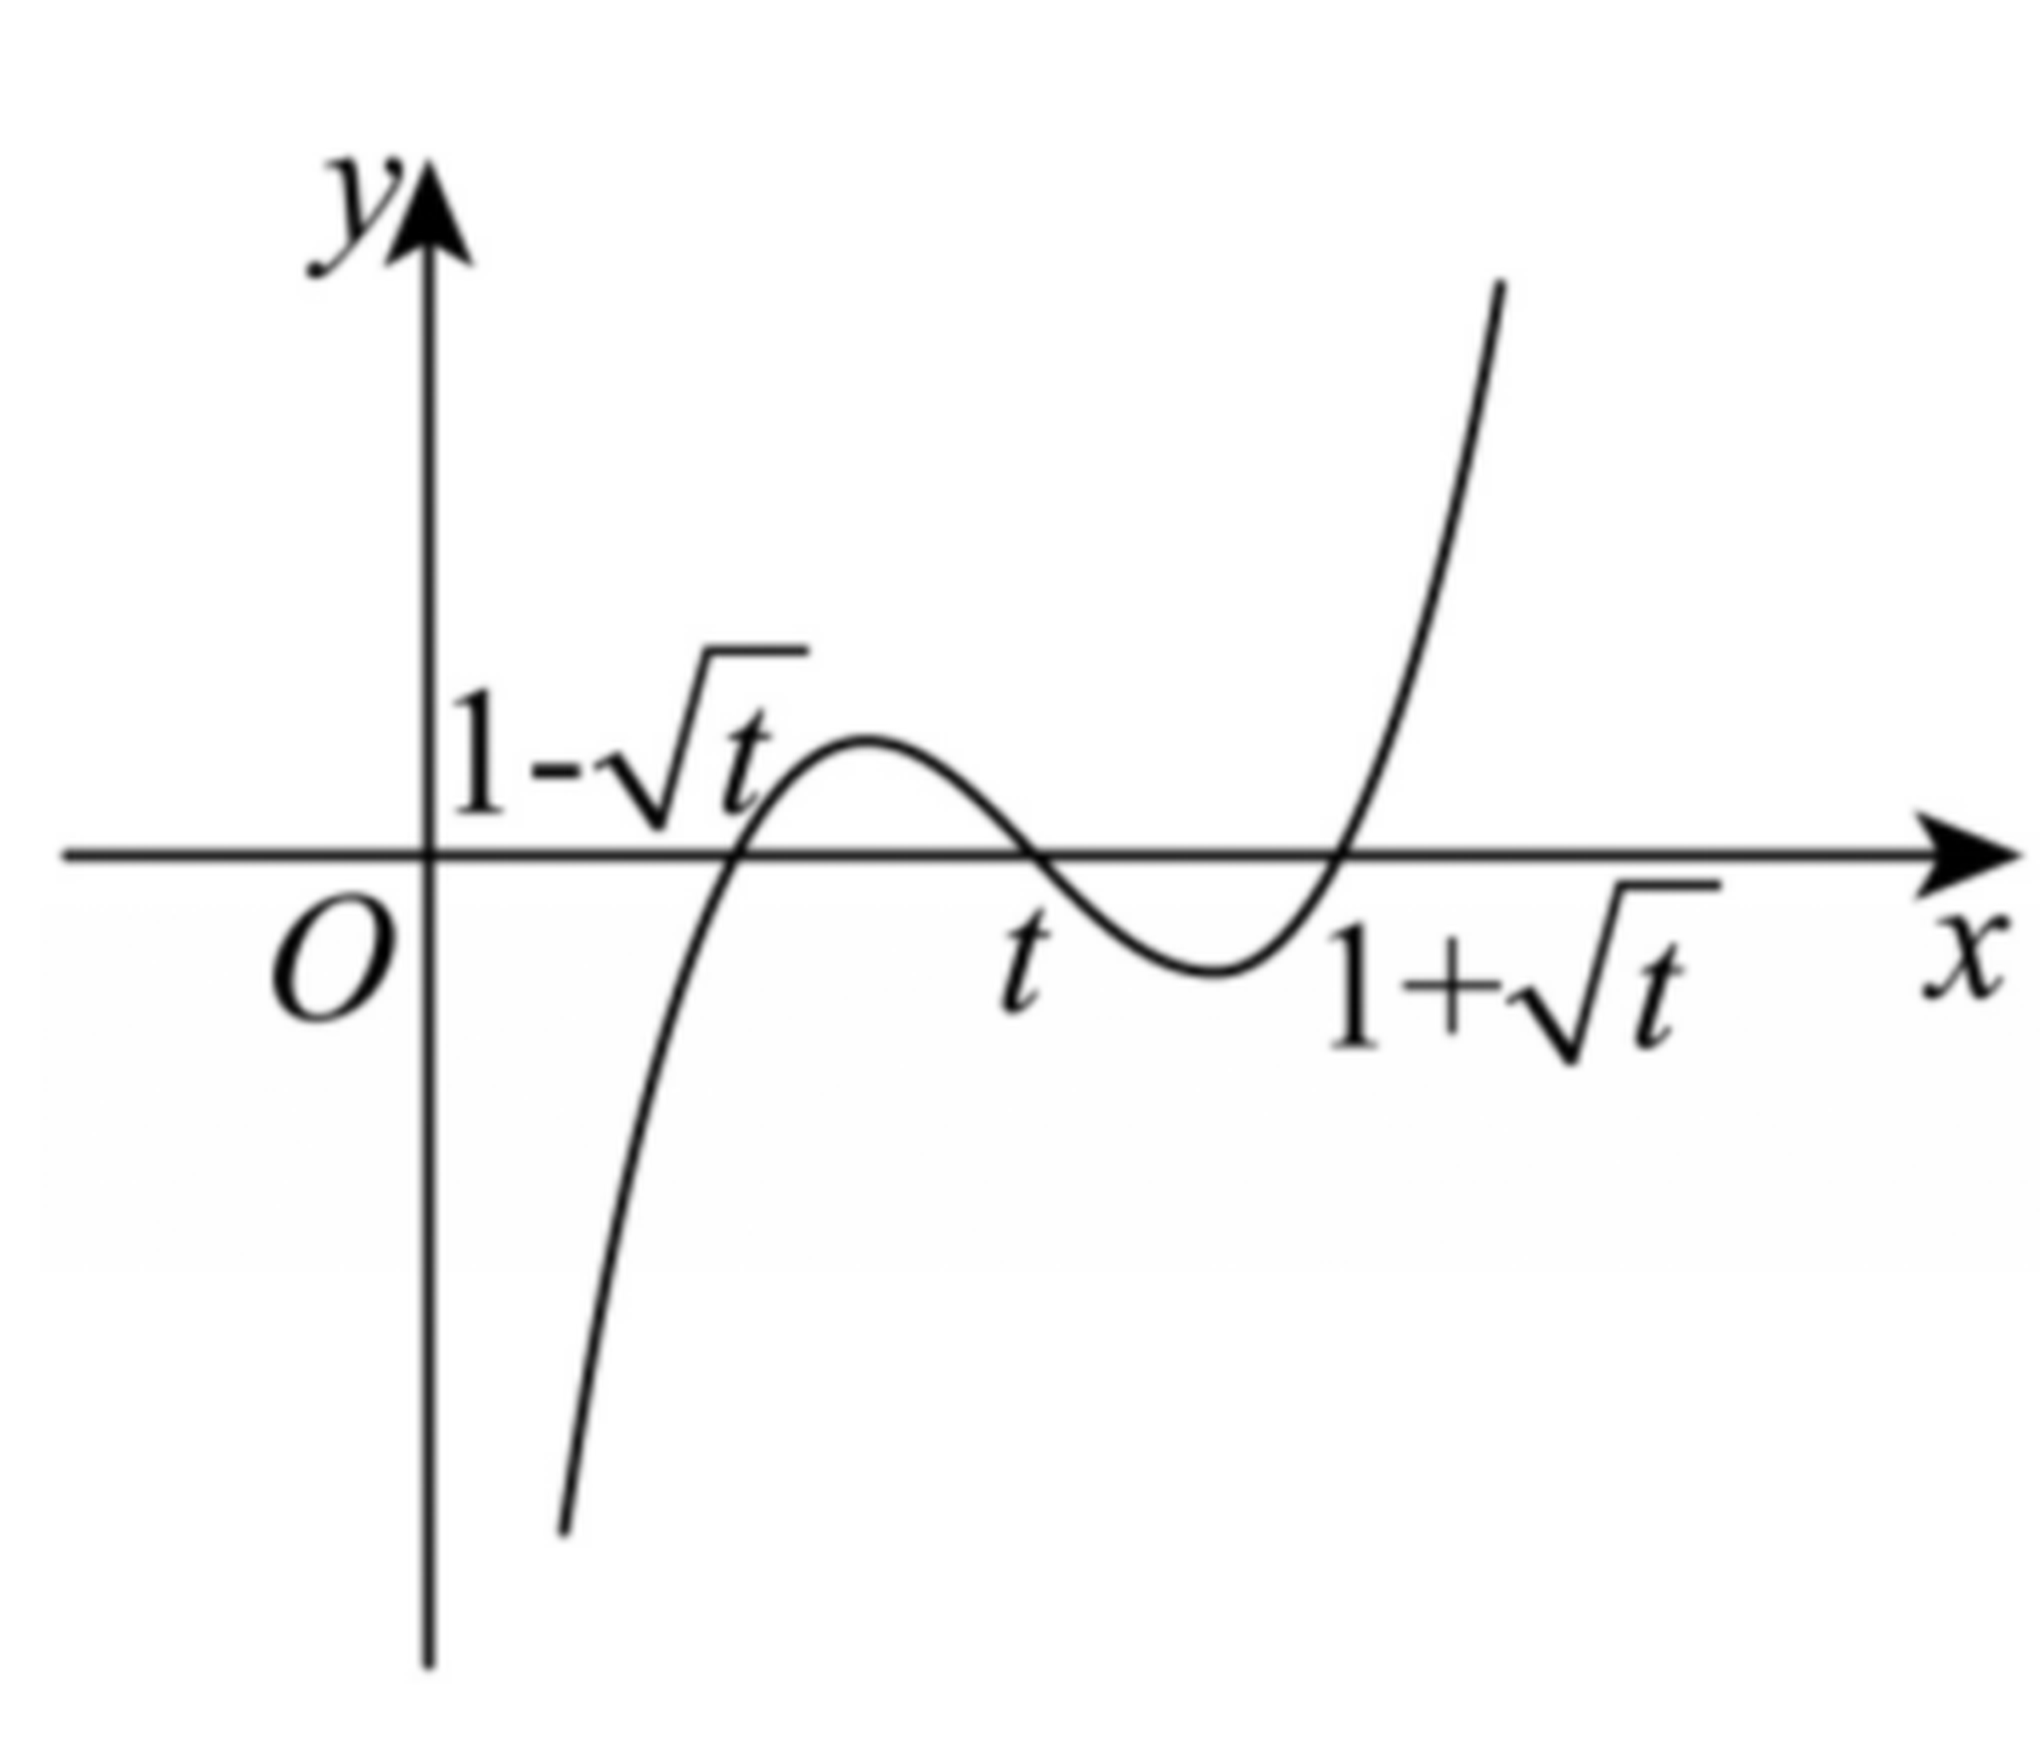
\includegraphics[width=0.40\textwidth]{figures/gao149_q12_c.png}
\end{center}
\step{则原不等式的解集为 $(-\infty,1-\sqrt t]\cup[t,1+\sqrt t]$，}
\step{当 $\begin{cases}1-\sqrt t>0\\1-\sqrt t\geqslant m\end{cases}$ 时，原不等式恒成立，此时 $t\in\left(\dfrac{3-\sqrt5}{2},1\right)$，$m\in\left(0,\dfrac{3-\sqrt5}{2}\right)$；}
\step{若 $t\geqslant1+\sqrt t$，即 $t\geqslant\dfrac{3+\sqrt5}{2}$，则取 $x=0$，$(t-1)t>0$，}
\step{原不等式不恒成立，不符合题意，}
\step{因此实数 $m$ 的取值范围是 $\left(0,\dfrac{\sqrt5+1}{2}\right]$，$m$ 的最大值是 $\dfrac{\sqrt5+1}{2}$.}
\solend
\fi

\end{enumerate}

\bigsec{二、选择题}

\begin{enumerate}
\setcounter{enumi}{12}

% === Q13 ===：答案"C"直接印在题干括号内、无【答案】/【解析】段，按 高一84 Q13／高一148 Q13 成例括号留空、另提 \ans{$C$}；四选项两行两列照原卷分行
\item 设 $ab>0$，则 $a>b$ 是 $\dfrac{1}{a}<\dfrac{1}{b}$ 的\mbox{（\quad）}

\keepwithprev
A. 充分不必要条件\qquad\qquad B. 必要不充分条件

C. 充要条件\qquad\qquad D. 既不充分又不必要条件

\ifanswer
\ans{$C$}
\fi

% === Q14 ===：$A\subset B$ 单线照录；四选项补集照原卷上划线 \overline{A}／\overline{B}；解析 1 行（由韦恩图得 B 对）
\item 已知集合 $A$、$B$ 非空，且 $A\subset B$，则下列式子中一定是空集的为\mbox{（\quad）}

\keepwithprev
A. $\overline{A}\cap B$\qquad B. $A\cap\overline{B}$\qquad C. $\overline{A}\cap\overline{B}$\qquad D. $\overline{A}\cup\overline{B}$

\ifanswer
\solbegin
\step{由韦恩图得 $B$ 对. 故选 $B$.}
\solend
\fi

% === Q15 ===："天文数字"弯引号照录；解析 2 行（首行在 04 页末、末行续 05 页顶）
\item 历史上数学计算方面的三大发明是阿拉伯数字、十进制和对数，其中对数的发明，大大缩短了计算时间，为人类研究科学和了解自然起了重大作用，对数运算对估算“天文数字”具有独特的优势. $2.5^{1000}$ 的估算值约为\mbox{（\quad）}

\keepwithprev
A. $10^{365}$\qquad B. $10^{379}$\qquad C. $10^{389}$\qquad D. $10^{398}$

\ifanswer
\solbegin
\step{$\lg 2.5^{1000}=1000\lg 2.5=1000(1-2\lg 2)\approx1000\times(1-0.602)=398$，}
\step{所以 $2.5^{1000}\approx10^{398}$. 故选 $D$.}
\solend
\fi

% === Q16 ===："完美集"新定义、圈数字①②文本模式；题干"若对任意 $x$，$y\in A$"用全角逗号、解析用顿号"$x$、$y\in A$"，两处照录不统一；解析 9 行
\item 设全集 $U=\R$，集合 $A$ 是一个非空数集，若对任意 $x$，$y\in A$，都有 $x+y\in A$、$xy\in A$，则称集合 $A$ 为一个“完美集”，给出以下命题：

①若 $A_1$、$A_2$ 都是“完美集”，且 $A_1\cap A_2\ne\varnothing$，则 $A_1\cap A_2$ 也是“完美集”；

②若 $A_1$、$A_2$ 都是“完美集”，则 $A_1\cup A_2$ 也是“完美集”.

下列说法正确的是\mbox{（\quad）}

\keepwithprev
A. ①②都是真命题\qquad\qquad B. ①是真命题，②是假命题

C. ①是假命题，②是真命题\qquad\qquad D. ①②都是假命题

\ifanswer
\solbegin
\step{由题意，全集 $U=\R$，集合 $A$ 是一个非空数集，}
\step{若对任意 $x$、$y\in A$，都有 $x+y\in A$、$xy\in A$，则称集合 $A$ 为一个“完美集”，}
\step{对于①，取 $x$、$y\in A_1\cap A_2$，则 $x\in A_1$，$x\in A_2$，$y\in A_1$，$y\in A_2$，}
\step{又 $A_1$、$A_2$ 是“完美集”，所以 $x+y\in A_1$，$xy\in A_1$，$x+y\in A_2$，$xy\in A_2$，}
\step{所以 $x+y\in A_1\cap A_2$，$xy\in A_1\cap A_2$，所以 $A_1\cap A_2$ 是“完美集”，故①正确；}
\step{对于②，取“完美集” $A_1=\{x\mid x=2k,k\in\Z\}$，$A_2=\{x\mid x=3k,k\in\Z\}$，}
\step{则 $2\in A_1$，$3\in A_2$，但 $2+3\notin A_1\cup A_2$，}
\step{即此时 $A_1\cup A_2$ 不是“完美集”，故②错误.}
\step{故选 $B$.}
\solend
\fi
\end{enumerate}

\bigsec{三、解答题}

\begin{enumerate}
\setcounter{enumi}{16}

% === Q17 ===："图像"（有亻）照录（Q17 题干与解析共 2 处）；绝对值 \lvert…\rvert；解析 7 行
\item 已知 $m\in\R$，$f(x)=(m^2-m-5)x^m$. 若 $y=f(x)$ 是幂函数，且其图像不经过原点.

(1) 求实数 $m$ 的值；

(2) 若 $f(a)=f(b)$ 且 $a\ne b$，求 $\lvert a+2\rvert+\lvert b-1\rvert$ 的最小值，并指出取到最小值时 $a$ 的取值范围.

\ifanswer
\solbegin
\step{(1) $f(x)=(m^2-m-5)x^m$ 是幂函数，得 $m^2-m-5=1$，即 $m^2-m-6=0$，}
\step{解得 $m=-2$ 或 $m=3$，又函数图像不经过原点，所以 $m=-2$($3$ 舍)；}
\step{(2) 由 (1) 得 $f(x)=x^{-2}=\dfrac{1}{x^2}$ 为偶函数，}
\step{$x<0$ 时，函数 $f(x)$ 严格增，$x>0$ 时，函数 $f(x)$ 严格减，}
\step{又 $f(a)=f(b)$ 且 $a\ne b$，所以 $a=-b$，且 $a\ne0$，$b\ne0$，}
\step{则 $\lvert a+2\rvert+\lvert b-1\rvert=\lvert a+2\rvert+\lvert-a-1\rvert=\lvert a+2\rvert+\lvert a+1\rvert$，}
\step{则 $\lvert a+2\rvert+\lvert b-1\rvert$ 的最小值为 $1$，取到最小值时 $a$ 的取值范围是 $[-2,-1]$.}
\solend
\fi

% === Q18 ===：判别式两形混用——(1) cases 块印高 \Delta、(2) 独立行印扁 \triangle，逐处照录不统一；解析 8 行
\item 已知命题 $p$：方程 $x^2+4x+m-1=0$ 有两个不等的负根；命题 $q$：方程 $4x^2+4x+m-2=0$ 无实根.

(1) 若 $p$ 为真命题，求 $m$ 的取值范围；

(2) 若 $p$、$q$ 两命题一真一假，求 $m$ 的取值范围.

\ifanswer
\solbegin
\step{(1) 若 $p$ 为真命题，即方程 $x^2+4x+m-1=0$ 有两个不等的负根；}
\step{必有 $\begin{cases}\Delta=16-4(m-1)>0\\m-1>0\end{cases}$，解得 $1<m<5$，即 $m$ 的取值范围为 $(1,5)$；}
\step{(2) 命题 $q$：方程 $4x^2+4x+m-2=0$ 无实根，}
\step{则有 $\triangle=16-16(m-2)<0$，解得 $m>3$，}
\step{若 $p$ 和 $q$ 有且只有一个为真命题，}
\step{若 $p$ 真 $q$ 假，必有 $\begin{cases}1<m<5\\m\leqslant3\end{cases}$，则有 $1<m\leqslant3$，}
\step{若 $p$ 假 $q$ 真，必有 $\begin{cases}m\leqslant1\text{ 或 }m\geqslant5\\m>3\end{cases}$，则有 $m\geqslant5$，}
\step{综上，$1<m\leqslant3$ 或 $m\geqslant5$.}
\solend
\fi

% === Q19 ===：$A\subseteq B$ 带下划线照录；解析 7 行（(2) 两组 cases 并排）
\item 已知 $m\in\R$，集合 $A=\left\{x\mid y=\sqrt{3-x}-\dfrac{1}{\sqrt{x-1}}\right\}$，集合 $B=\{x\mid 2m\leqslant x\leqslant1-m\}$.

(1) 若 $A\cup B=B$，求实数 $m$ 的取值范围；

(2) 若 $A\cap B=\varnothing$，求实数 $m$ 的取值范围.

\ifanswer
\solbegin
\step{(1) 函数 $y=\sqrt{3-x}-\dfrac{1}{\sqrt{x-1}}$，则 $\begin{cases}3-x\geqslant0\\x-1>0\end{cases}$，解得 $1<x\leqslant3$，}
\step{所以 $A=\{x\mid1<x\leqslant3\}$，}
\step{因为 $A\cup B=B$，所以 $A\subseteq B$，则 $\begin{cases}2m\leqslant1\\1-m\geqslant3\end{cases}$，解得 $m\leqslant-2$，}
\step{综上，实数 $m$ 的取值范围为 $(-\infty,-2]$；}
\step{(2) 当 $B=\varnothing$ 时，则 $2m>1-m$，解得 $m>\dfrac{1}{3}$，}
\step{当 $B\ne\varnothing$ 时，则 $\begin{cases}2m\leqslant1-m\\2m>3\end{cases}$ 或 $\begin{cases}2m\leqslant1-m\\1-m\leqslant1\end{cases}$，解得 $m\in\varnothing$ 或 $0\leqslant m\leqslant\dfrac{1}{3}$，}
\step{综上，实数 $m$ 的取值范围为 $[0,+\infty)$.}
\solend
\fi

% === Q20 ===：n 阶基本不等式推广；(3) 解析含 \overbrace{…}^{k} 上括号；(2) 解析"x=x=x=3(1-x)"三连等系原卷笔误、照录加注（见 ⑤）；解析 14 行
\item 教材中的基本不等式可以推广到 $n$ 阶：$n$ 个正数的算术平均数不小于它们的几何平均数，即对于任意的正数 $a_1$、$a_2$、$\cdots$、$a_n$，有 $\dfrac{a_1+a_2+\cdots+a_n}{n}\geqslant\sqrt[n]{a_1\cdot a_2\cdots a_n}$（$n\in\N$ 且 $n\geqslant2$），且等号当且仅当 $a_1=a_2=\cdots=a_n$ 时成立. 利用此结论解决下列问题：

(1) 若 $x$、$y$、$z>0$，求 $\dfrac{y}{x}+\dfrac{2z}{y}+\dfrac{4x}{z}$ 的最小值；

(2) 已知 $0<x<1$，求 $x^3(1-x)$ 的最大值，并求取得最大值时的 $x$ 的值；

(3) 对任意的正整数 $k$，判断 $\left(1+\dfrac{1}{k}\right)^k$ 与 $\left(1+\dfrac{1}{k+1}\right)^{k+1}$ 的大小关系，并证明.

\ifanswer
\solbegin
\step{(1) 因为 $x$、$y$、$z>0$，有 $\dfrac{y}{x}>0$，$\dfrac{2z}{y}>0$，$\dfrac{4x}{z}>0$}
\step{所以 $\dfrac{y}{x}+\dfrac{2z}{y}+\dfrac{4x}{z}\geqslant3\sqrt[3]{\dfrac{y}{x}\cdot\dfrac{2z}{y}\cdot\dfrac{4x}{z}}=3\sqrt[3]{8}=6$，}
\step{当且仅当 $\dfrac{y}{x}=\dfrac{2z}{y}=\dfrac{4x}{z}$ 时取等号，故 $\dfrac{y}{x}+\dfrac{2z}{y}+\dfrac{4x}{z}$ 的最小值为 $6$.}
\step{(2) 因为 $0<x<1$，所以 $1-x>0$，}
\step{$x^3(1-x)=\dfrac{1}{3}[x\cdot x\cdot x\cdot3(1-x)]\leqslant\dfrac{1}{3}\left[\dfrac{x+x+x+3(1-x)}{4}\right]^4=\dfrac{1}{3}\times\left(\dfrac{3}{4}\right)^4$}
\step{$=\dfrac{27}{256}$，当且仅当 $x=x=x=3(1-x)$，即 $x=3(1-x)$，$x=\dfrac{3}{4}$ 取等号，}% 原卷"x=x=x=3(1-x)"三连等，疑为四因子相等之误排，放大 08 页确认，照录未改（见 ⑤）
\step{所以 $0<x<1$ 时，$x^3(1-x)$ 的最大值是 $\dfrac{27}{256}$，取最大值时 $x=\dfrac{3}{4}$.}
\step{(3) 对任意 $k\in\N^*$，$\left(1+\dfrac{1}{k}\right)^k<\left(1+\dfrac{1}{k+1}\right)^{k+1}$.}
\step{证明：$\left(1+\dfrac{1}{k}\right)^k=\overbrace{\left(1+\dfrac{1}{k}\right)\cdot\left(1+\dfrac{1}{k}\right)\cdots\left(1+\dfrac{1}{k}\right)}^{k}\times1$}
\step{$\leqslant\left(\dfrac{\overbrace{\left(1+\dfrac{1}{k}\right)+\left(1+\dfrac{1}{k}\right)+\cdots+\left(1+\dfrac{1}{k}\right)}^{k}+1}{k+1}\right)^{k+1}$}
\step{$=\left(\dfrac{\overbrace{(1+1+\cdots+1)}^{k}+\overbrace{\left(\dfrac{1}{k}+\dfrac{1}{k}+\cdots+\dfrac{1}{k}\right)}^{k}+1}{k+1}\right)^{k+1}=\left(\dfrac{k+1+1}{k+1}\right)^{k+1}=\left(1+\dfrac{1}{k+1}\right)^{k+1}$，}
\step{当且仅当 $1+\dfrac{1}{k}=1$ 时取等号，}
\step{但是任意 $k\in\N^*$ 时 $1+\dfrac{1}{k}>1$，所以等号不成立，}
\step{故任意 $k\in\N^*$ 时，$\left(1+\dfrac{1}{k}\right)^k<\left(1+\dfrac{1}{k+1}\right)^{k+1}$.}
\solend
\fi

% === Q21 ===："减 k 集"新定义（引号内 k／数字两侧空格照录）；解析 26 行（续 10 页），含 ⑤ 三处原卷笔误照录
\item 定义：对于给定的整数 $k$，若非空集合 $A$ 满足如下 3 个条件：

① $A$ 是正整数集的子集；② $A\ne\{1\}$；

③对任意正整数 $x,y$，若 $x+y\in A$，则 $xy-k\in A$；则称集合 $A$ 为“减 $k$ 集”.

(1) 判断集合 $A=\{1,2\}$ 是否为“减 $0$ 集”？是否为“减 $1$ 集”？（无需说明理由）

(2) 证明：不存在“减 $2$ 集”；

(3) 是否存在“减 $1$ 集”？如果存在，求出所有“减 $1$ 集”；如果不存在，说明理由.

\ifanswer
\solbegin
\step{(1) 因为 $P\subseteq\N^*$，$P\ne\{1\}$，$1+1=2\in P$，$1\times1-0\in P$，}
\step{所以集合 $P=\{1,2\}$ 是“减 $0$ 集”；}
\step{因为 $P\subseteq\N^*$，$P\ne\{1\}$，$1+1=2\in P$，$1\times1-1\notin P$，}
\step{所以集合 $P=\{1,2\}$ 是“减 $1$ 集”；}% 按条件③应为"不是"，原卷径印"是"，放大 09 页确认，照录未改（见 ⑤）
\step{(2) 假设存在集合 $A$ 是“减 $2$ 集”，若 $x+y\in A$，则 $xy-2\in A$，}
\step{①当 $x+y=xy-2$ 时，有 $(x-1)(y-1)=3$，}
\step{则 $x$、$y$ 一个为 $2$，一个为 $4$，所以集合 $A$ 有元素 $6$，}
\step{但 $3+3\in A$，$3\times3-2\notin A$，与 $A$ 是“减 $2$ 集”矛盾；}
\step{②当 $x+y\ne xy-2$ 时，则 $x+y=xy-1$ 或 $x+y=xy-m$($m>2$)，}
\step{若 $x+y=xy-1$，$m=1$ 时，$M$ 为除 $1$ 以外的最小元素，}% 原卷"m=1"上文未显式定义，疑笔误，放大 09 页确认，照录未改（见 ⑤）
\step{则 $x=M-1$，$y=1$ 时，$xy-2=M-3$ 小于 $M$，}
\step{要符合题意，必须 $M=4$，}
\step{此时取 $x-2$，$y=2$，$xy-2=2$ 不属于 $A$，故不符合题意，}% 原卷"取 x−2"疑为"取 x=2"误排，放大 09 页确认，照录未改（见 ⑤）
\step{当 $m>2$ 时，$(x-1)(y-1)=m+1$，同样得出矛盾，}
\step{综上，不存在 $A$ 是“减 $2$ 集”.}
\step{(3) 存在“减 $1$ 集” $A$，则 $A\ne\{1\}$，}
\step{①假设 $1\in A$，则 $A$ 中除了元素 $1$ 以外，必然还含有其它元素，}
\step{假设 $2\in A$，$1+1\in A$，而 $1\times1-1\notin A$，所以 $2\notin A$，}
\step{假设 $3\in A$，$1+2\in A$，而 $1\times2-1\in A$，所以 $3\in A$，}
\step{所以 $A=\{1,3\}$，}
\step{假设 $4\in A$，$1+3\in A$，而 $1\times3-1\notin A$，所以 $4\notin A$，}
\step{假设 $5\in A$，$1+4\in A$，$1\times4-1\in A$，$2+3=5$，$2\times3-1\in A$，所以 $5\in A$，}
\step{所以 $A=\{1,3,5\}$，}
\step{以此类推，得 $A=\{1,3,5,\cdots,2n-1,\cdots\}$，($n\in\N^*$)，}
\step{所以所有的“减 $1$ 集”有 $\{1,3\}$，$\{1,3,5\}$，$\{1,3,5,7\}$，$\cdots$，$\{1,3,5,\cdots,2n-1,\cdots\}$，}
\step{$(n\in\N^*)$.}
\solend
\fi
\end{enumerate}

\end{document}
"
%
% ① 原始材料：微信公众号"魔都数学加油站"文章，连载"27学年高一149"，原文标题
% "27学年高一149——2026-2027年上海市青浦高级中学上外云间高一上期中"；
% 原文链接：https://mp.weixin.qq.com/s/T7_nyoR1k0o_5og7FkDsyw 。
% 正文为 10 张 PNG 页（01/02/03/04/10 为 2560×3620，05/06/07/08/09 为 4762×6735，
% 同一篇各页分辨率混排，逐页按各自分辨率裁图核对，别按预览比例换算裁框）。
% 体例：混合体例讲评版——19 题中 Q6 只印【答案】、无【解析】；Q13 的答案"C"
%   直接印在题干括号内、无【答案】/【解析】段；其余 17 题印【解析】（逐题核实，见 ② ②）。
% 题目、答案、解析均据原图转录；卷面粉红色水印"魔都数学加油站"及公众号页脚未录入。
% 全卷插图清单（逐页通读 10 页确认）：1 幅题目配图 + 3 幅【解析】内配图：
%   · Q11 矩形 ABCD 折叠几何图（02 页右侧：A/B/C/D/E/F/C' 与虚线 EB、BC、FC），
%     题干"如图"处，题目配图、三版都出，裁 figures/gao149_q11.png；
%   · Q12【解析】内 3 幅三次函数曲线坐标图（03 页右侧两幅 + 04 页右侧一幅：
%     x/y 轴、O、t、1-\sqrt t、1+\sqrt t 等标注，分别对应 t<1-\sqrt t、
%     t=1-\sqrt t、1+\sqrt t>t>1-\sqrt t 三种情形），解析配图、仅答案版出，
%     分别裁 figures/gao149_q12_a.png／_b.png／_c.png，放 \ifanswer 内 \step 之间
%     （高一73 第 16 题成例）；
%   其余各页逐页确认无其它题目配图、无表格；Q14 解析"由韦恩图得 B 对"仅文字推导、
%   原卷并未印韦恩图；Q9／Q18／Q19 的 cases 块与 Q20(3) 的 \overbrace 为数学块（非图）；
%   10 页下半仅水印、无正文。4 图均取自原卷截图，去粉色水印、去色、4× LANCZOS 放大。
%
% 卷首标题：原卷印作"2026-2027 年青浦高级中学上外云间高一上期中"，年份区间按全稿
% 惯例排 en dash；原卷卷面未印副标题，本稿按同期中卷（高一140／141／143／144／145／
% 146／147／148）知识模块口径补出"集合与常用逻辑用语、不等式、函数"。
%
% 题号体例（逐页核实定稿）：本卷共 19 题——一、填空题 3—12（10 题）、
% 二、选择题 13—16（4 题）、三、解答题 17—21（5 题）。
% 三节分别 \setcounter{enumi}{2}／{12}／{16}。原卷从第 3 题起、无第 1、2 题，
% 本稿保留原题号；全卷无附加题节（Q21 解析末行"（n\in N^*）."为全卷收尾）。
%
% ② 与原卷的排版差异：
%   ① 原文从第 3 题起，本稿保留原题号；共 19 题三节；
%   ② 混合体例逐题核实：Q6（反证法"假设的内容"）只印【答案】、无【解析】，
%      按 高一140 第 5 题／高一145 Q3 成例提 \ans{}、不补造解析；Q13 答案"C"直接
%      印在题干括号内、全卷无该题【答案】/【解析】段，按 高一84 Q13／高一148 Q13
%      成例括号 \mbox{（\quad）} 留空、另提 \ans{$C$}；其余 17 题印【解析】、
%      用 \solbegin…\solend，选择题答案在解析末句"故选 X"（Q14 选 B、Q15 选 D、
%      Q16 选 B，逐个放大 04/05 页核实）、题干括号留空、不另提 \ans{}；
%      答案版【答案】/【解析】标记数 = 19（2 个 \ans ＋ 17 个 \solbegin）
%      = 全卷题数；
%   ③ 原卷卷面未印副标题，本稿按知识模块口径补出；
%   ④ 原卷填空横线按全稿惯例排 \blankline[4.4em]；选择题括号排 \mbox{（\quad）}、
%      选项段前按惯例加 \keepwithprev；Q13／Q16 四选项为两行两列、Q14／Q15
%      选项为一行，照原卷分行；解答题不留作答区、不加 \anspace（原卷为讲评版）；
%   ⑤ 数集：Q6"a,b\in N"、Q8"x\in R"、Q9"a\in R"／"解集为 R"、Q12"t\in R"、
%      Q16"U=R"、Q17"m\in R"、Q19"m\in R"、Q20"n\in N" 原卷印斜体 R/N，
%      按全稿惯例统一改 \R／\N；Q20(3)、Q21 的 $N^*$ 排 \N^*；Q16 解析
%      "$k\in Z$" 排 \Z。绝对值排 \lvert…\rvert（Q17），集合描述竖线排 \mid
%      （Q19、Q16 解析）；不等号按全稿惯例排 \leqslant／\geqslant；
%      补集照原卷上划线排 \overline{A}／\overline{B}（Q14 四选项）；空集
%      \varnothing（Q16、Q19、Q21）；
%   ⑥ 子集符号逐处照录不统一：Q4 题干"{1,2}⊆A⊂{1,2,3,4,5,6}" 前者印带下划线
%      ⊆、照录 \subseteq，后者印单线 ⊂、照录 \subset；Q10"A⊆{-1,1/2,2,3}"、
%      Q19 解析"A⊆B"、Q21 解析"P⊆N*" 均印带下划线 ⊆、照录 \subseteq；
%      Q14"A⊂B" 印单线 ⊂、照录 \subset（逐处放大 01/02/04/07/09 页确认，见 ④）；
%   ⑦ 子题标号 (1)(2)(3) 半角括号照录；圈数字 ①②③ 在文本模式（Q16 两命题、
%      Q21 三个条件与解析的①②）按 common.sty 划入 CJK 字符类渲染；cases 块整体
%      算一个印刷行；\left…\right 不得拆到不同 $…$ 组；数学式内 CJK 用 \text{}
%      （Q18 解析 cases 块"\text{或}"）；Q11 解析"Rt\triangle DC'F" 的 Rt 照录；
%   ⑧ 题干／解析中的中文弯引号按原卷照录：Q6" 已知 a,b\in N，若 ab 能被 5 整除，
%      那么 a、b 中至少有一个能被 5 整除 "（开引号后紧跟"已知"、闭引号后空格接"时"）、
%      Q15"天文数字"、Q16"完美集"、Q21"减 k 集""减 0 集""减 1 集""减 2 集"
%      （引号内 k／数字两侧有空格），注释内一律 ASCII 引号；
%   ⑨ 半角逗号在数学组之间是全稿惯例、非笔误（Q8"$a>0,a\ne1,x\in\R$"、
%      Q21 题干"$x,y$" 等），逐处照录别改；Q16 题干"若对任意 $x$，$y\in A$"
%      用全角逗号而解析用顿号"$x$、$y\in A$"，两处不同均照录；行末西文句点
%      照录为 ASCII `.`；行中全角逗号／顿号照录；
%   ⑩ "图像／图象"逐处放大核：Q10 题干与解析共 6 处均印"图象"（象，无亻）；
%      Q17 题干"其图像不经过原点"与解析"又函数图像不经过原点" 2 处印"图像"
%      （像，有亻），逐处照录未统一改动（放大 02/05/06 页确认）；
%   ⑪ 判别式 Δ/△ 混用是照录项：Q9 解析 cases 块"Δ=4(a−2)²+16(a−2)<0"、
%      Q18(1) cases 块"Δ=16−4(m−1)>0" 两处印等腰偏高粗三角 \Delta；
%      Q18(2) 独立行"△=16−16(m−2)<0" 印扁等边细线三角 \triangle，
%      逐处放大判断、照录不统一（参照 高一142／144／145／146／148 头注④口径）；
%      另 Q11 题干"△C'DF 面积"与解析 3 处"△"（含"Rt△DC'F"）共 4 处几何
%      三角形符号亦印扁细线三角，照录 \triangle（非判别式，字形同类，见 ④）；
%   ⑫ 一条 \step = 原卷解析的一个印刷行，cases 块整体算一个印刷行；别把原卷折行
%      并起来、别把一行拆多条。Q11 十三行（7 行在 02 页＋6 行在 03 页）、
%      Q12 十五行（8 行在 03 页＋7 行在 04 页）、Q16 九行、Q21 二十六行
%      （续 10 页）均按印刷行逐条断，不丢行；
%   ⑬ 配图：Q11 题目配图（三版都出）放 \item 内题干之后 \begin{center}，
%      大图块加 \needvspace{8cm} 守卫把整块推走（守卫放 \item 之前，见
%      高一145 Q14/Q20 成例与切页审计 B 类坑）；Q12 三幅解析配图（仅答案版出）
%      放 \ifanswer 内 \solbegin…\solend 的 \step 之间；三版切页审计均"合计异常：无"；
%   ⑭ 跨页续印按题合并：Q3/4/5 在 01 页；Q6/7/8 题干与解析在 01 页；
%      Q9 题干在 01 页末、解析 4 行在 02 页顶；Q10 题干＋解析在 02 页；
%      Q11 题干＋图＋解析前 7 行在 02 页、解析后 6 行续 03 页顶；
%      Q12 题干＋解析首行在 03 页末、解析续 7 行在 03 页下半＋7 行在 04 页顶，
%      "二、选择题"标题在 04 页下半；Q13/14 题干＋选项＋Q14 解析在 04 页下半；
%      Q15 题干＋选项＋解析首行在 04 页末、末行"所以 2.5^1000≈10^398. 故选 D."
%      续 05 页顶；Q16 题干＋选项＋解析 9 行在 05 页、"三、解答题"标题＋
%      Q17 题干首句在 05 页末；Q17(2)＋解析 7 行、Q18 题干＋解析前 6 行在 06 页；
%      Q18 解析末 2 行续 07 页顶；Q19 题干＋解析 4 行在 07 页上半、
%      解析续 3 行在 07 页下半；Q20 题干(1) 在 07 页末、题干(2)(3)＋解析(1)(2)
%      在 08 页上半、(3) 解析含 \overbrace 的证明在 08 页下半、末行
%      "故任意 k∈N* 时…"续 09 页顶；Q21 题干＋解析(1)(2)(3) 前段在 09 页、
%      解析(3) 后半 9 行续 10 页上半（10 页下半仅水印、无正文）。
%      本稿按题连排，不丢行、不并折行；
%   ⑮ 原卷解析内无红色"法一／法二"之类小标题，故本卷无 \stepm；水印
%      "魔都数学加油站"红色不录入。
%
% ③ 行数复核：一条 \step／\stepm = 原卷解析的一个印刷行，cases 块作一个印刷行计。
%   逐题数（主会话逐页核对定稿）：Q3：1；Q4：2；Q5：2；Q6：0（只印【答案】、
%   提 \ans{}）；Q7：1；Q8：1；Q9：4；Q10：5；Q11：13；Q12：15；
%   Q13：0（答案印在题干括号内、另提 \ans{}）；Q14：1；Q15：2；Q16：9；
%   Q17：7；Q18：8；Q19：7；Q20：14；Q21：26。
%   合计 118 条 \step（本卷无 \stepm：解析内无红色"法一／法二"类小标题），
%   与原卷逐题印刷行相等。全卷 17 题设 \solbegin…\solend ＋ 2 处 \ans{}，
%   答案版【答案】/【解析】标记数 = 19 = 全卷题数。
%
% ④ 判别式／子集符号结论（逐处放大原图照录、不得统一，主会话像素级复核）：
%   判别式全卷 3 处，两形混用逐处照录不统一（参照 高一142／144／145／146／148 头注④）：
%     · Q9 解析 cases 块"Δ=4(a−2)²+16(a−2)<0" 原卷印等腰偏高粗三角（高>宽、
%       粗笔画），照录 \Delta（放大 02 页 /tmp/gao149/z/t02_q9_delta2.png 确认）；
%     · Q18(1) cases 块"Δ=16−4(m−1)>0" 原卷印等腰偏高粗三角（高>宽、粗笔画），
%       照录 \Delta（放大 06 页 /tmp/gao149/z/t06_q18a.png 确认）；
%     · Q18(2) 独立行"△=16−16(m−2)<0" 原卷印扁等边细线三角（宽>高、细线），
%       照录 \triangle（放大 06 页 /tmp/gao149/z/t06_q18b.png 与 Q18(1) 并排确认）。
%   另 Q11 题干"△C'DF"与解析 3 处"△"（含"Rt△DC'F"）共 4 处几何三角形符号
%     亦印扁等边细线三角，照录 \triangle（放大 02 页
%     /tmp/gao149/z/t02_q11_tri2.png 确认），与 Q9／Q18(1) 判别式 \Delta 两形不统一。
%   子集／补集：Q4 题干"{1,2}⊆A⊂{1,2,3,4,5,6}" 前者带下划线 ⊆、照录 \subseteq，
%     后者单线 ⊂、照录 \subset（放大 01 页 /tmp/gao149/z/t01_q3q4.png 确认）；
%     Q10"A⊆{-1,1/2,2,3}"、Q19 解析"A⊆B"、Q21 解析"P⊆N*" 三处带下划线 ⊆、
%     照录 \subseteq；Q14"A⊂B" 单线 ⊂、照录 \subset（放大 04 页
%     /tmp/gao149/z/t04_q14_sub2.png 确认）；Q14 四选项补集 \overline{A}／\overline{B}
%     照原卷上划线；空集 \varnothing（Q16、Q19、Q21）；Q19／Q16 解析集合描述竖线
%     \mid；数集 \R／\N／\N^*／\Z 归一见 ② ⑤。
%
% ⑤ 存疑照录（放大原图确认，照录未改、正文对应处另有 % 注）：
%   1. Q21 解析(1) 第二组"因为 P⊆N*，P≠{1}，1+1=2∈P，1×1−1∉P，所以集合
%      P={1,2} 是"减 1 集"" —— 按条件③（x=y=1 时 xy−1=0 须∈P）应为"不是"，
%      原卷却径印"是"，放大 09 页 /tmp/gao149/z/t09_q21_sol1.png 确认，照录未改
%      （疑为原卷结论笔误）。
%   2. Q21 解析(2)"此时取 x−2，y=2，xy−2=2 不属于 A" —— 按上下文应为
%      "取 x=2"（x−2 疑为 x=2 的误排），放大 09 页
%      /tmp/gao149/z/t09_q21_sol2.png 确认，照录未改。
%   3. Q21 解析(2)"若 x+y=xy−1，m=1 时，M 为除 1 以外的最小元素" 中 $m=1$
%      上文未显式定义 m（仅"x+y=xy−m(m>2)"中出现），放大 09 页确认，照录未改。
%   4. Q20 解析(2)"当且仅当 x=x=x=3(1−x)" 三个 x 连等，疑为原卷排印（应为
%      四个因子 x,x,x,3(1−x) 相等），放大 08 页
%      /tmp/gao149/z/t08_q20_sol2.png 确认，照录未改。
%   5. Q6 只印【答案】、Q13 答案印题干括号内，两题均无【解析】，按成例提
%      \ans{}、未补造解析（见 ② ②）。
%   6. 判别式 Q9／Q18(1) 高 \Delta 与 Q18(2)／Q11 扁 \triangle 两形混用，逐处
%      照录不统一（见 ④）；"图像／图象" Q10 用"图象"、Q17 用"图像"，
%      逐处照录未统一（见 ② ⑩）。
%   全卷除此 6 类外未发现其它笔误／自相矛盾处。
%
% ⑥ 跨页续印按题合并说明：见 ② ⑭。
%
\documentclass[a4paper,11pt]{article}
\usepackage{common}

\begin{document}

\examtitlest[3]{2026--2027 年青浦高级中学上外云间高一上期中}{集合与常用逻辑用语、不等式、函数}

\bigsec{一、填空题}

\begin{enumerate}
\setcounter{enumi}{2}

% === Q3 === 根式化分数指数幂；解析 1 行
\item 根式 $\sqrt{a\sqrt a}$ 化成分数指数幂是\blankline[4.4em].

\ifanswer
\solbegin
\step{$\sqrt{a\sqrt a}=\sqrt{a\cdot a^{\frac{1}{2}}}=\sqrt{a^{1+\frac{1}{2}}}=\sqrt{a^{\frac{3}{2}}}=a^{\frac{3}{2}\times\frac{1}{2}}=a^{\frac{3}{4}}$.}
\solend
\fi

% === Q4 === 题干两种子集符号逐处照录（\subseteq 带下划线／\subset 单线）；解析 2 行
\item 满足 $\{1,2\}\subseteq A\subset\{1,2,3,4,5,6\}$ 的集合 $A$ 共有\blankline[4.4em]个.

\ifanswer
\solbegin
\step{集合 $A$ 满足 $\{1,2\}\subseteq A\subset\{1,2,3,4,5,6\}$，}% 前者带下划线 $\subseteq$、后者单线 $\subset$，逐处照录不统一（放大 01 页确认）
\step{所以集合 $A$ 的个数为集合 $\{3,4,5,6\}$ 的真子集的个数，即为 $2^4-1=15$ 个.}
\solend
\fi

% === Q5 === 解析 2 行
\item 不等式 $\dfrac{2x+1}{x-1}\leqslant0$ 的解集为\blankline[4.4em].

\ifanswer
\solbegin
\step{不等式 $\dfrac{2x+1}{x-1}\leqslant0$ 可化为 $(2x+1)(x-1)\leqslant0$，且 $x-1\ne0$，解得 $-\dfrac{1}{2}\leqslant x<1$，}
\step{即原不等式的解集为 $\left[-\dfrac{1}{2},1\right)$.}
\solend
\fi

% === Q6 === 原卷只印【答案】、无【解析】，按 高一140 第 5 题／高一145 Q3 成例提 \ans{}、不补造解析；弯引号与空格照录
\item 用反证法证明命题 “已知 $a,b\in\N$，若 $ab$ 能被 5 整除，那么 $a$、$b$ 中至少有一个能被 5 整除” 时，假设的内容应该是\blankline[4.4em].

\ifanswer
\ans{$a$、$b$ 都不能被 5 整除}
\fi

% === Q7 === 解析 1 行
\item 若 $\log_3(\log_4 x)=1$，则 $x=$\blankline[4.4em].

\ifanswer
\solbegin
\step{$\log_3(\log_4 x)=1$，则 $\log_4 x=3$，故 $x=64$.}
\solend
\fi

% === Q8 === 半角逗号在数学组之间照录；解析 1 行
\item 已知 $a>0,a\ne1,x\in\R$，且 $a^{2x}=2$，则 $\dfrac{a^{3x}+a^{-3x}}{a^x+a^{-x}}$ 的值为\blankline[4.4em].

\ifanswer
\solbegin
\step{$\dfrac{a^{3x}+a^{-3x}}{a^x+a^{-x}}=a^{2x}-1+a^{-2x}=2-1+\dfrac{1}{2}=\dfrac{3}{2}$.}
\solend
\fi

% === Q9 === 题干在 01 页末、解析 4 行在 02 页顶；cases 块整体算 1 行；判别式高 \Delta
\item 已知 $a\in\R$，若关于 $x$ 的不等式 $(a-2)x^2+2(a-2)x-4<0$ 的解集为 $\R$，则实数 $a$ 的取值范围是\blankline[4.4em].

\ifanswer
\solbegin
\step{当 $a=2$ 时，不等式化为 $-4<0$ 对于任意实数 $x$ 都成立，因此 $a=2$ 满足题意；}
\step{当 $a\ne2$ 时，要使关于 $x$ 的不等式 $(a-2)x^2+2(a-2)x-4<0$ 的解集为 $\R$，}
\step{则 $\begin{cases}a-2<0\\\Delta=4(a-2)^2+16(a-2)<0\end{cases}$，解得 $-2<a<2$.}% cases 块整体算一个印刷行；判别式原卷印等腰偏高粗三角 $\Delta$，照录（放大 02 页确认）
\step{综上，$a$ 的取值范围为 $(-2,2]$.}
\solend
\fi

% === Q10 === "图象"（象，无亻）逐处照录；\subseteq 带下划线；解析 5 行
\item 已知集合 $A=\{\alpha,\beta\}$，且 $A\subseteq\left\{-1,\dfrac{1}{2},2,3\right\}$，函数 $f(x)=x^\alpha$ 与 $g(x)=x^\beta$ 的图象有两个交点，则满足条件的不同集合 $A$ 有\blankline[4.4em]个.

\ifanswer
\solbegin
\step{函数 $y=x^{-1}$ 与 $y=x^{\frac{1}{2}}$，$y=x^2$，$y=x^3$ 的图象分别有 1 个，1 个，2 个交点；}
\step{函数 $y=x^{\frac{1}{2}}$ 与 $y=x^2$，$y=x^3$ 的图象都有 2 个交点；}
\step{函数 $y=x^2$ 与 $y=x^3$ 的图象有 2 个交点，}
\step{函数 $f(x)=x^\alpha$ 与 $g(x)=x^\beta$ 的图象若只有 2 个交点，}
\step{则 $A=\{-1,3\}$ 或 $\left\{\dfrac{1}{2},2\right\}$ 或 $\left\{\dfrac{1}{2},3\right\}$ 或 $\{2,3\}$，有 4 个.}
\solend
\fi

% === Q11 === 题目配图（矩形折叠，三版都出）；\needvspace{8cm} 守卫放 \item 之前；解析 13 行（7 行 02 页＋6 行 03 页）
\needvspace{8cm}
\item 如图，矩形 $ABCD(AB>AD)$ 的周长为 12，在 $AB$ 和 $CD$ 边上分别取点 $E$ 和 $F$，将四边形 $BCFE$ 沿 $EF$ 折叠，使点 $B$ 与点 $D$ 重合，此时点 $C$ 的对应点为 $C'$，则 $\triangle C'DF$ 面积的最大值为\blankline[4.4em].

\begin{center}
% 矩形 ABCD 折叠几何图取 02 页右侧，去粉色水印、去色、4× LANCZOS 放大；三版都出
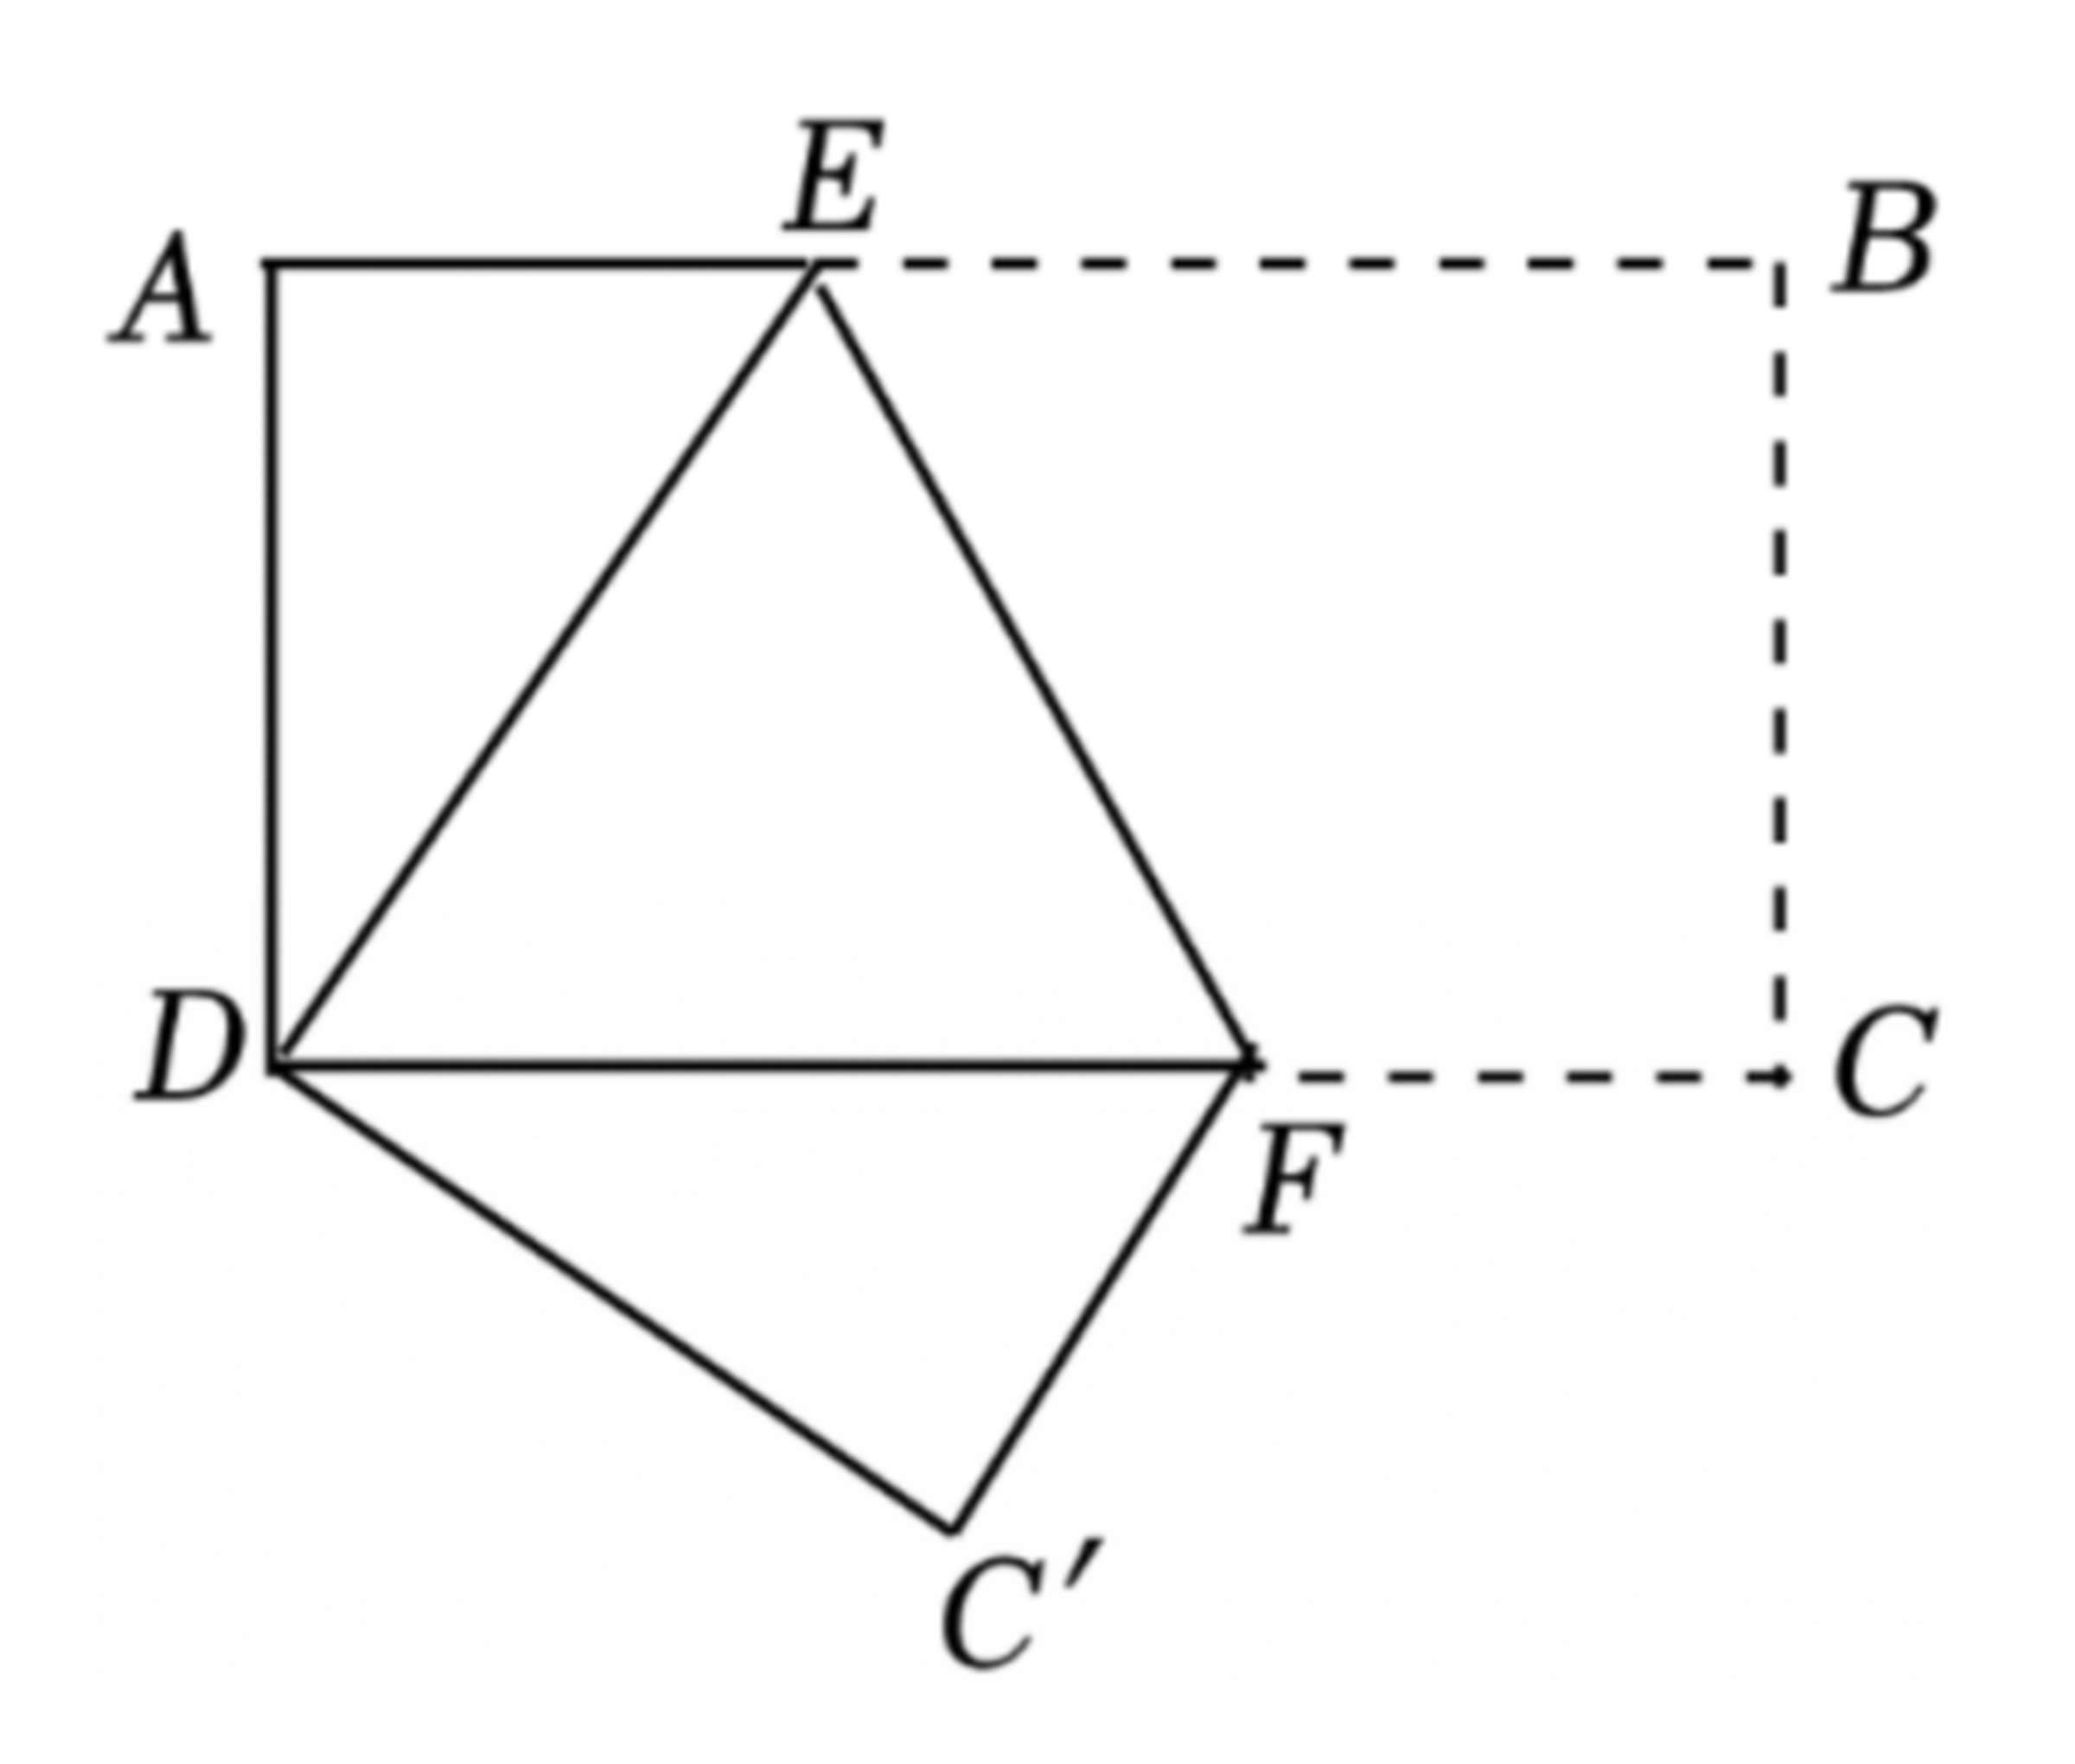
\includegraphics[width=0.40\textwidth]{figures/gao149_q11.png}
\end{center}

\ifanswer
\solbegin
\step{因为矩形 $ABCD(AB>AD)$ 的周长为 12，}
\step{在 $AB$ 和 $CD$ 边上分别取点 $E$ 和 $F$，将四边形 $BCFE$ 沿 $EF$ 折叠，}
\step{使点 $B$ 与点 $D$ 重合，此时点 $C$ 的对应点为 $C'$，}
\step{所以设 $AD=a$，$AB=b$，则 $2(a+b)=12$，}
\step{所以 $a+b=6$，且 $AB>AD$，所以 $b>a>0$，}
\step{设 $DF=x$，则 $C'F=b-x$，在 $Rt\triangle DC'F$ 中，$DC'=BC=a$，}% 几何三角形符号原卷印扁等边细线三角 $\triangle$，照录（放大 02 页确认）；$Rt$ 照录
\step{所以 $a^2+(b-x)^2=x^2$，解得 $x=\dfrac{a^2+b^2}{2b}$，}
\step{因此 $\triangle C'DF$ 的面积 $S=\dfrac{1}{2}\cdot DC'\cdot C'F=\dfrac{1}{2}\cdot a\cdot(b-x)$，}
\step{又 $b-x=b-\dfrac{(6-b)^2+b^2}{2b}=\dfrac{6(b-3)}{b}$，}
\step{所以 $S=\dfrac{1}{2}\cdot a\cdot\dfrac{6(b-3)}{b}=\dfrac{1}{2}\cdot(6-b)\cdot\dfrac{6(b-3)}{b}=\dfrac{3(6-b)(b-3)}{b}$}
\step{$=3\cdot\left(-b-\dfrac{18}{b}+9\right)$，又 $b+\dfrac{18}{b}\geqslant2\sqrt{b\cdot\dfrac{18}{b}}=6\sqrt{2}$，}
\step{当且仅当 $b=\dfrac{18}{b}$ 即 $b=3\sqrt{2}$ 时取等号，此时满足 $b>a$，}
\step{所以 $S\leqslant3\cdot(-6\sqrt{2}+9)=27-18\sqrt{2}$，故 $\triangle C'DF$ 面积的最大值为 $27-18\sqrt{2}$.}
\solend
\fi

% === Q12 === 解析内 3 幅三次函数曲线坐标图（仅答案版出）；解析 15 行（8 行 03 页＋7 行 04 页）
\item 已知 $m>0$，若存在 $t\in\R$，使得对任意 $x\in[0,m]$，不等式 $[(x-1)^2-t](x-t)\leqslant0$ 恒成立，则 $m$ 的最大值是\blankline[4.4em].

\ifanswer
\solbegin
\step{当 $t\leqslant0$ 时，$(x-1)^2-t\geqslant0$ 恒成立，}
\step{不等式 $[(x-1)^2-t](x-t)\leqslant0$ 的解集为 $x\leqslant t$，与 $x\in[0,m]$ 矛盾；}
\step{当 $t>0$ 时，不等式 $[(x-1)^2-t](x-t)\leqslant0\Leftrightarrow(x-1-\sqrt t)(x-1+\sqrt t)(x-t)\leqslant0$，}
\step{若 $t<1-\sqrt t$，即 $t\in\left(0,\dfrac{3-\sqrt5}{2}\right)$，}
\begin{center}
% 情形一 $t<1-\sqrt t$ 曲线图取 03 页右侧，去粉色水印、去色、4× LANCZOS 放大；仅答案版出
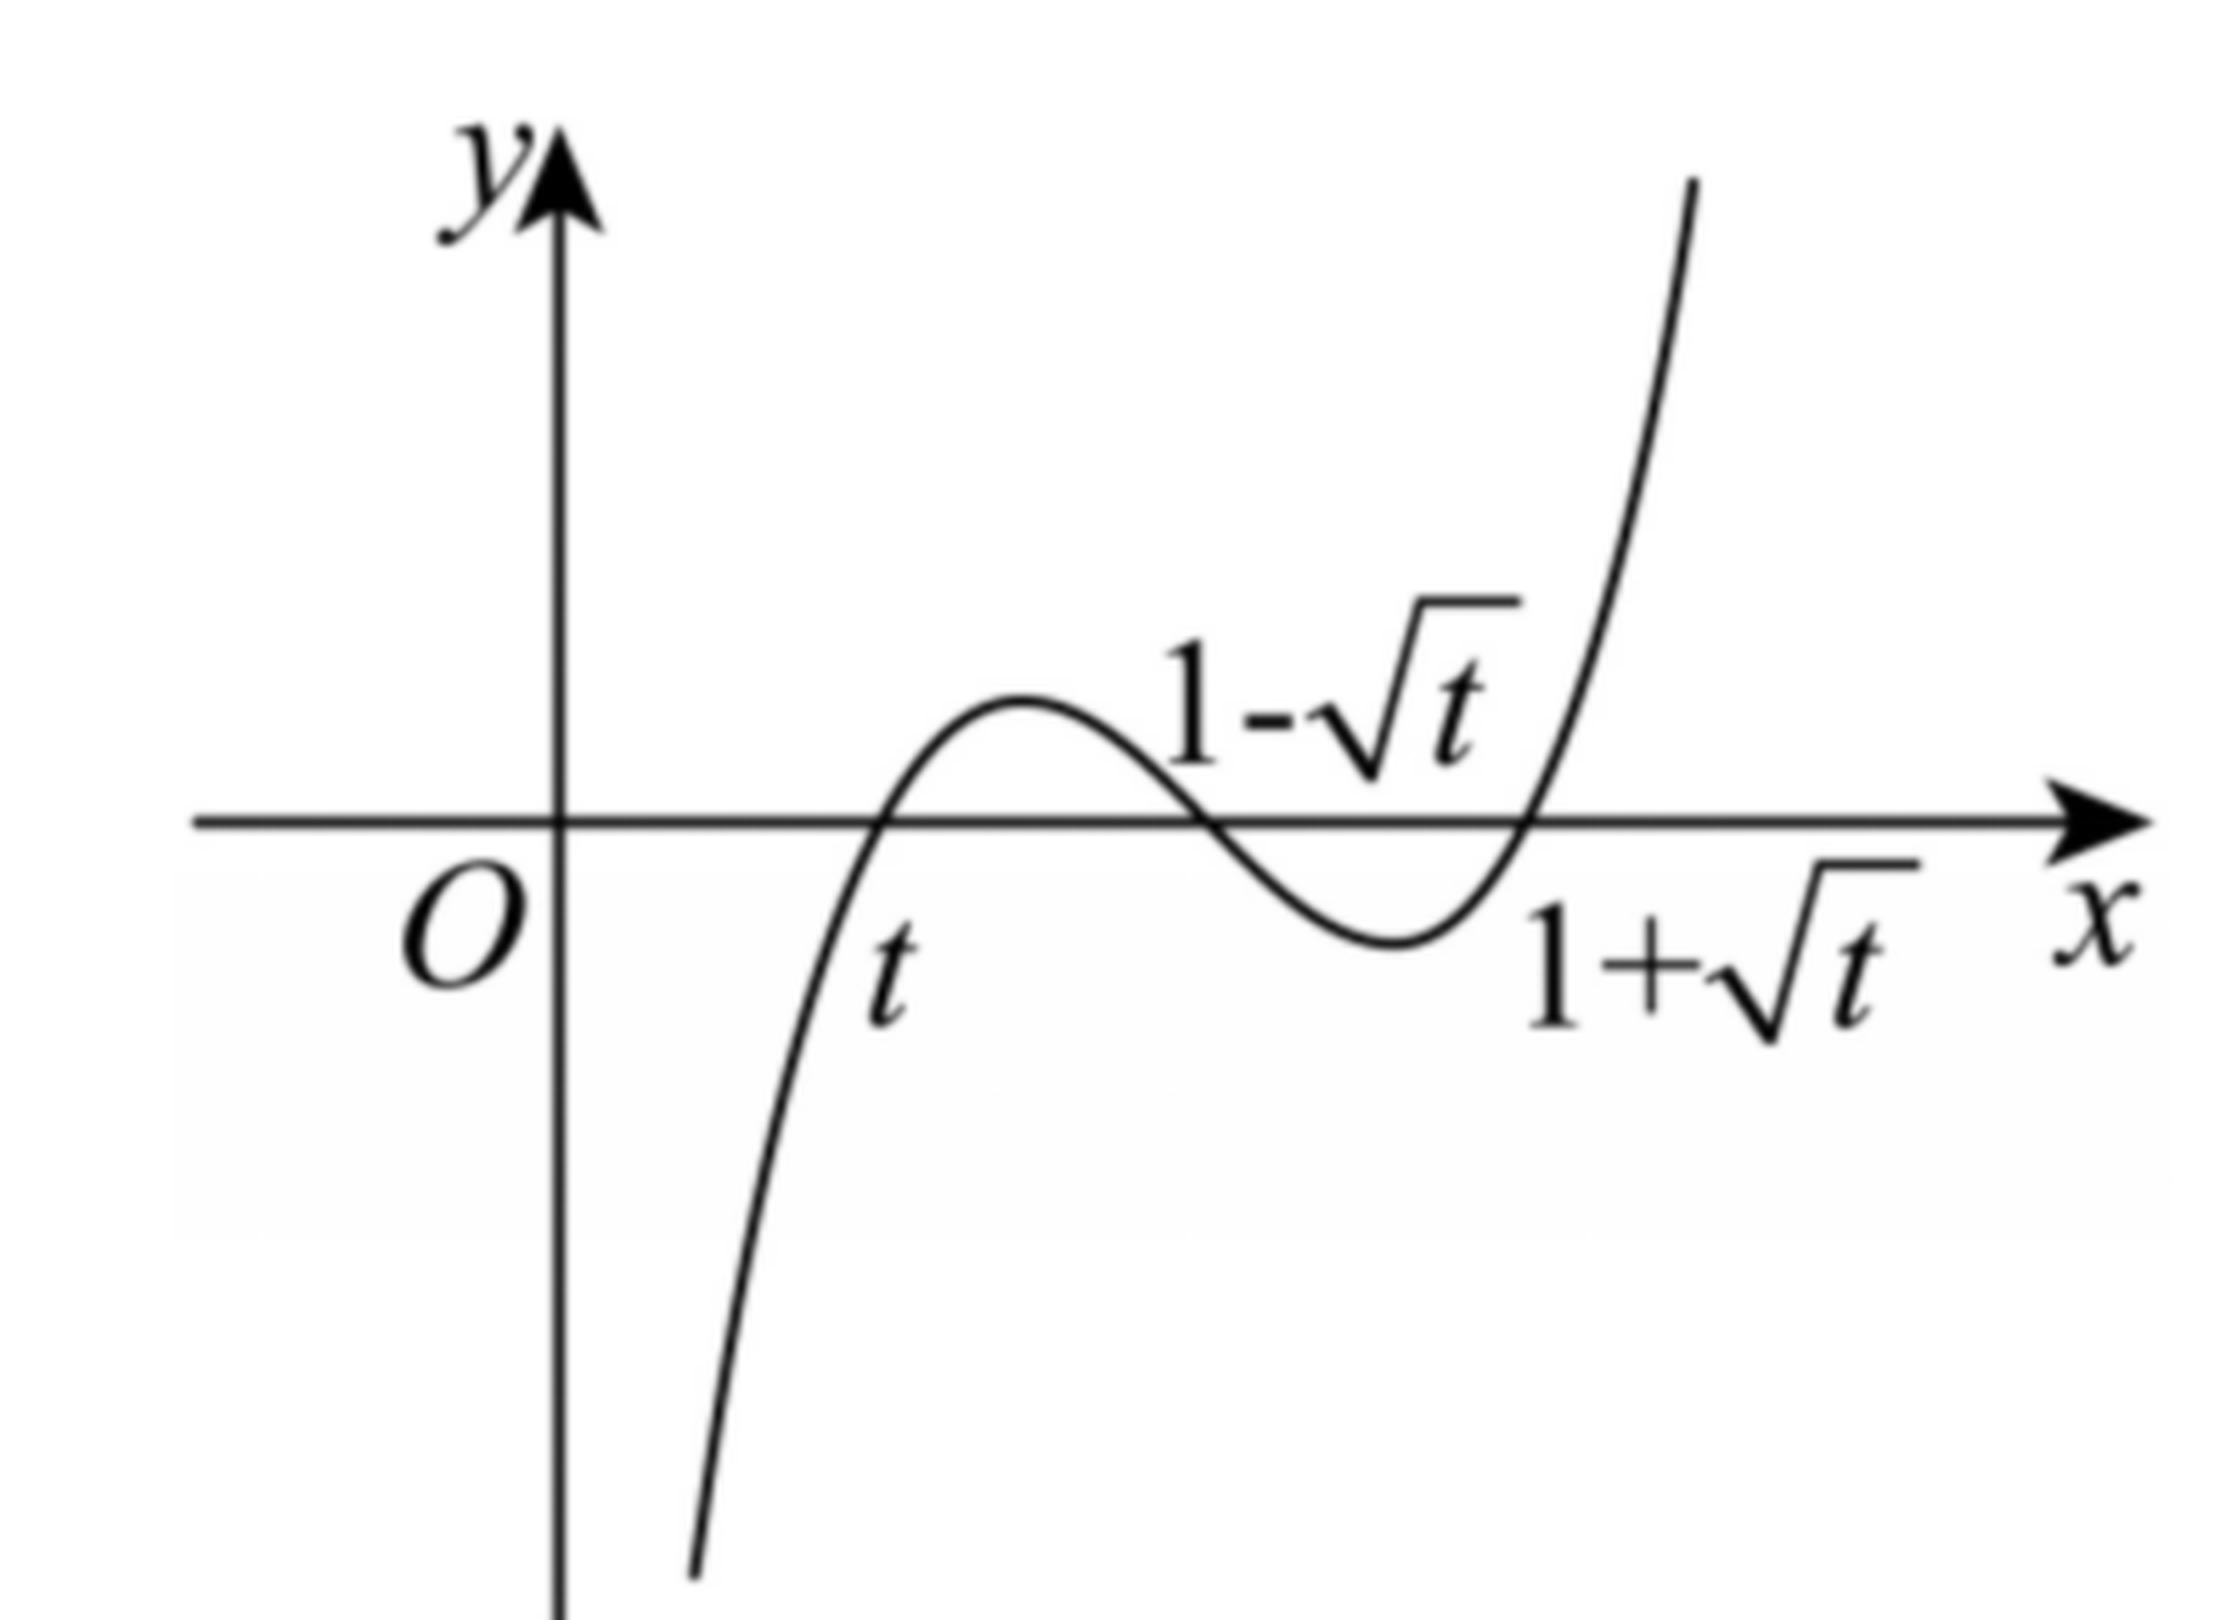
\includegraphics[width=0.40\textwidth]{figures/gao149_q12_a.png}
\end{center}
\step{则原不等式的解集为 $(-\infty,t]\cup[1-\sqrt t,1+\sqrt t]$，}
\step{当 $0<m\leqslant t$ 时，原不等式恒成立，因此}
\step{$m\in\left(0,\dfrac{3-\sqrt5}{2}\right)$；}
\step{若 $t=1-\sqrt t$，即 $t=\dfrac{3-\sqrt5}{2}$，则原不等式的解集为 $(-\infty,1+\sqrt t]$，}
\begin{center}
% 情形二 $t=1-\sqrt t$ 曲线图取 03 页右侧，去粉色水印、去色、4× LANCZOS 放大；仅答案版出
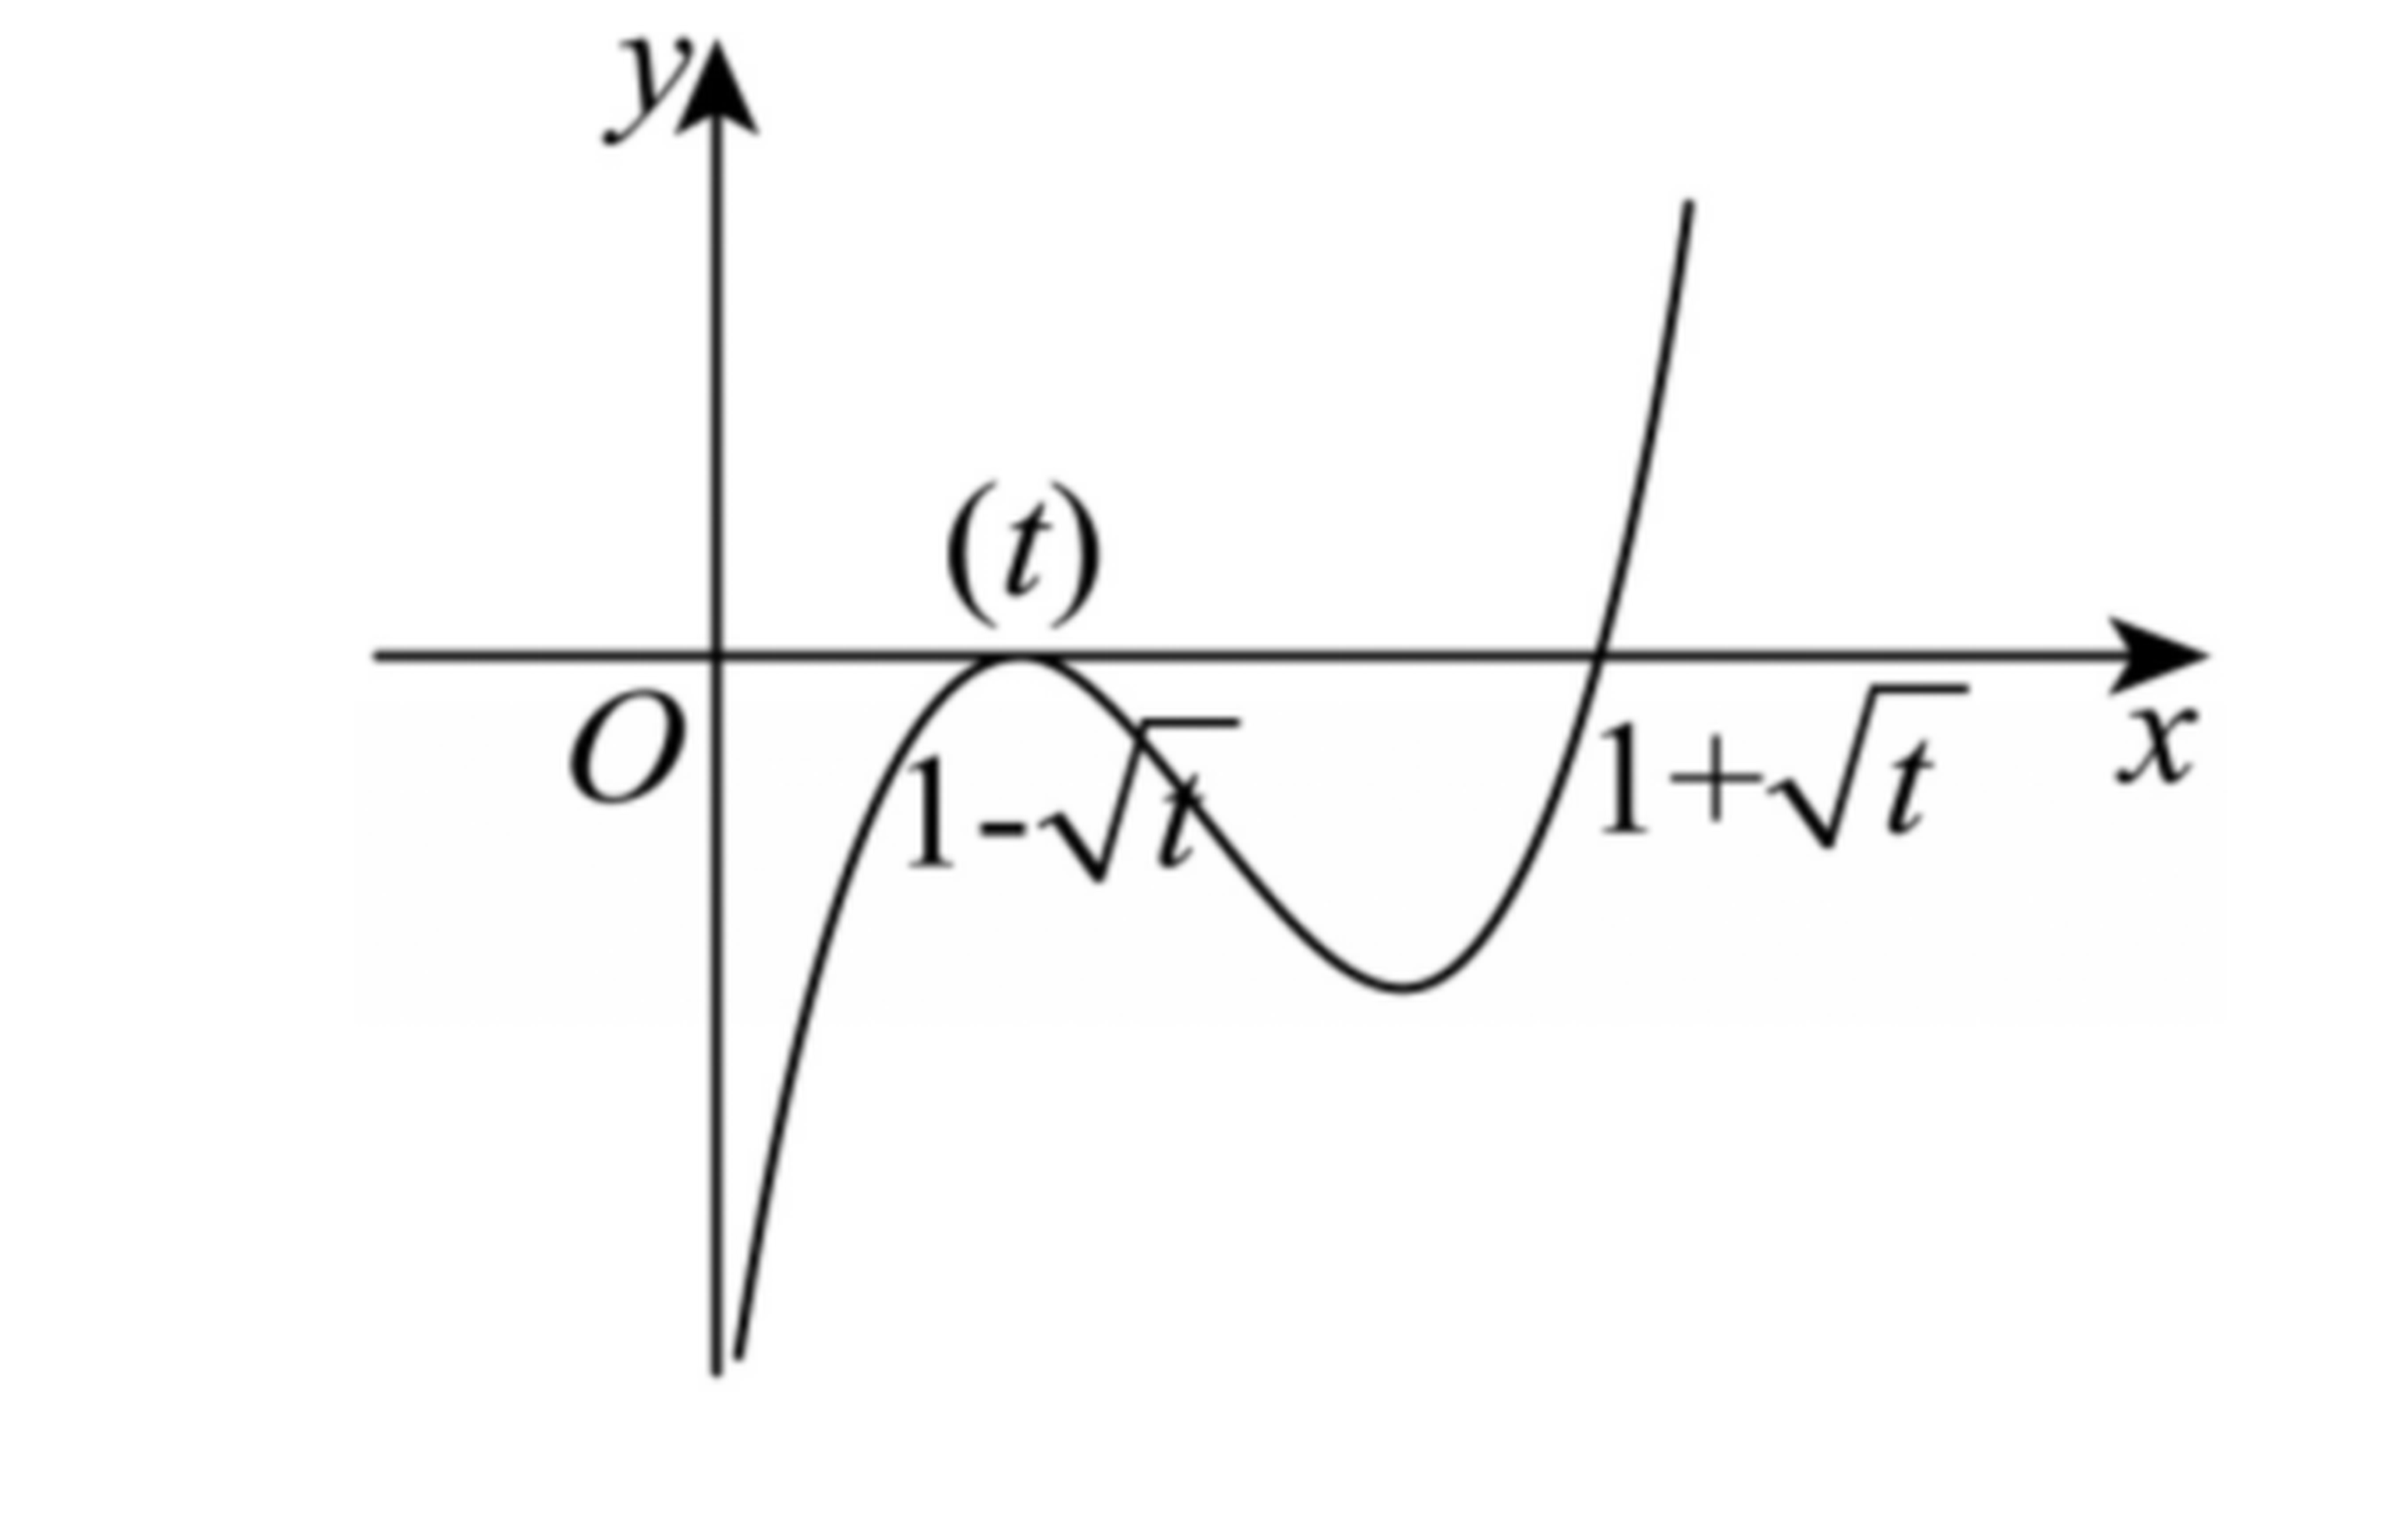
\includegraphics[width=0.40\textwidth]{figures/gao149_q12_b.png}
\end{center}
\step{当 $0<m\leqslant1+\sqrt t$ 时，原不等式恒成立，因此 $m\in\left(0,\dfrac{\sqrt5+1}{2}\right]$；}
\step{若 $1+\sqrt t>t>1-\sqrt t$，即 $t\in\left(\dfrac{3-\sqrt5}{2},\dfrac{3+\sqrt5}{2}\right)$，}
\begin{center}
% 情形三 $1+\sqrt t>t>1-\sqrt t$ 曲线图取 04 页右侧，去粉色水印、去色、4× LANCZOS 放大；仅答案版出
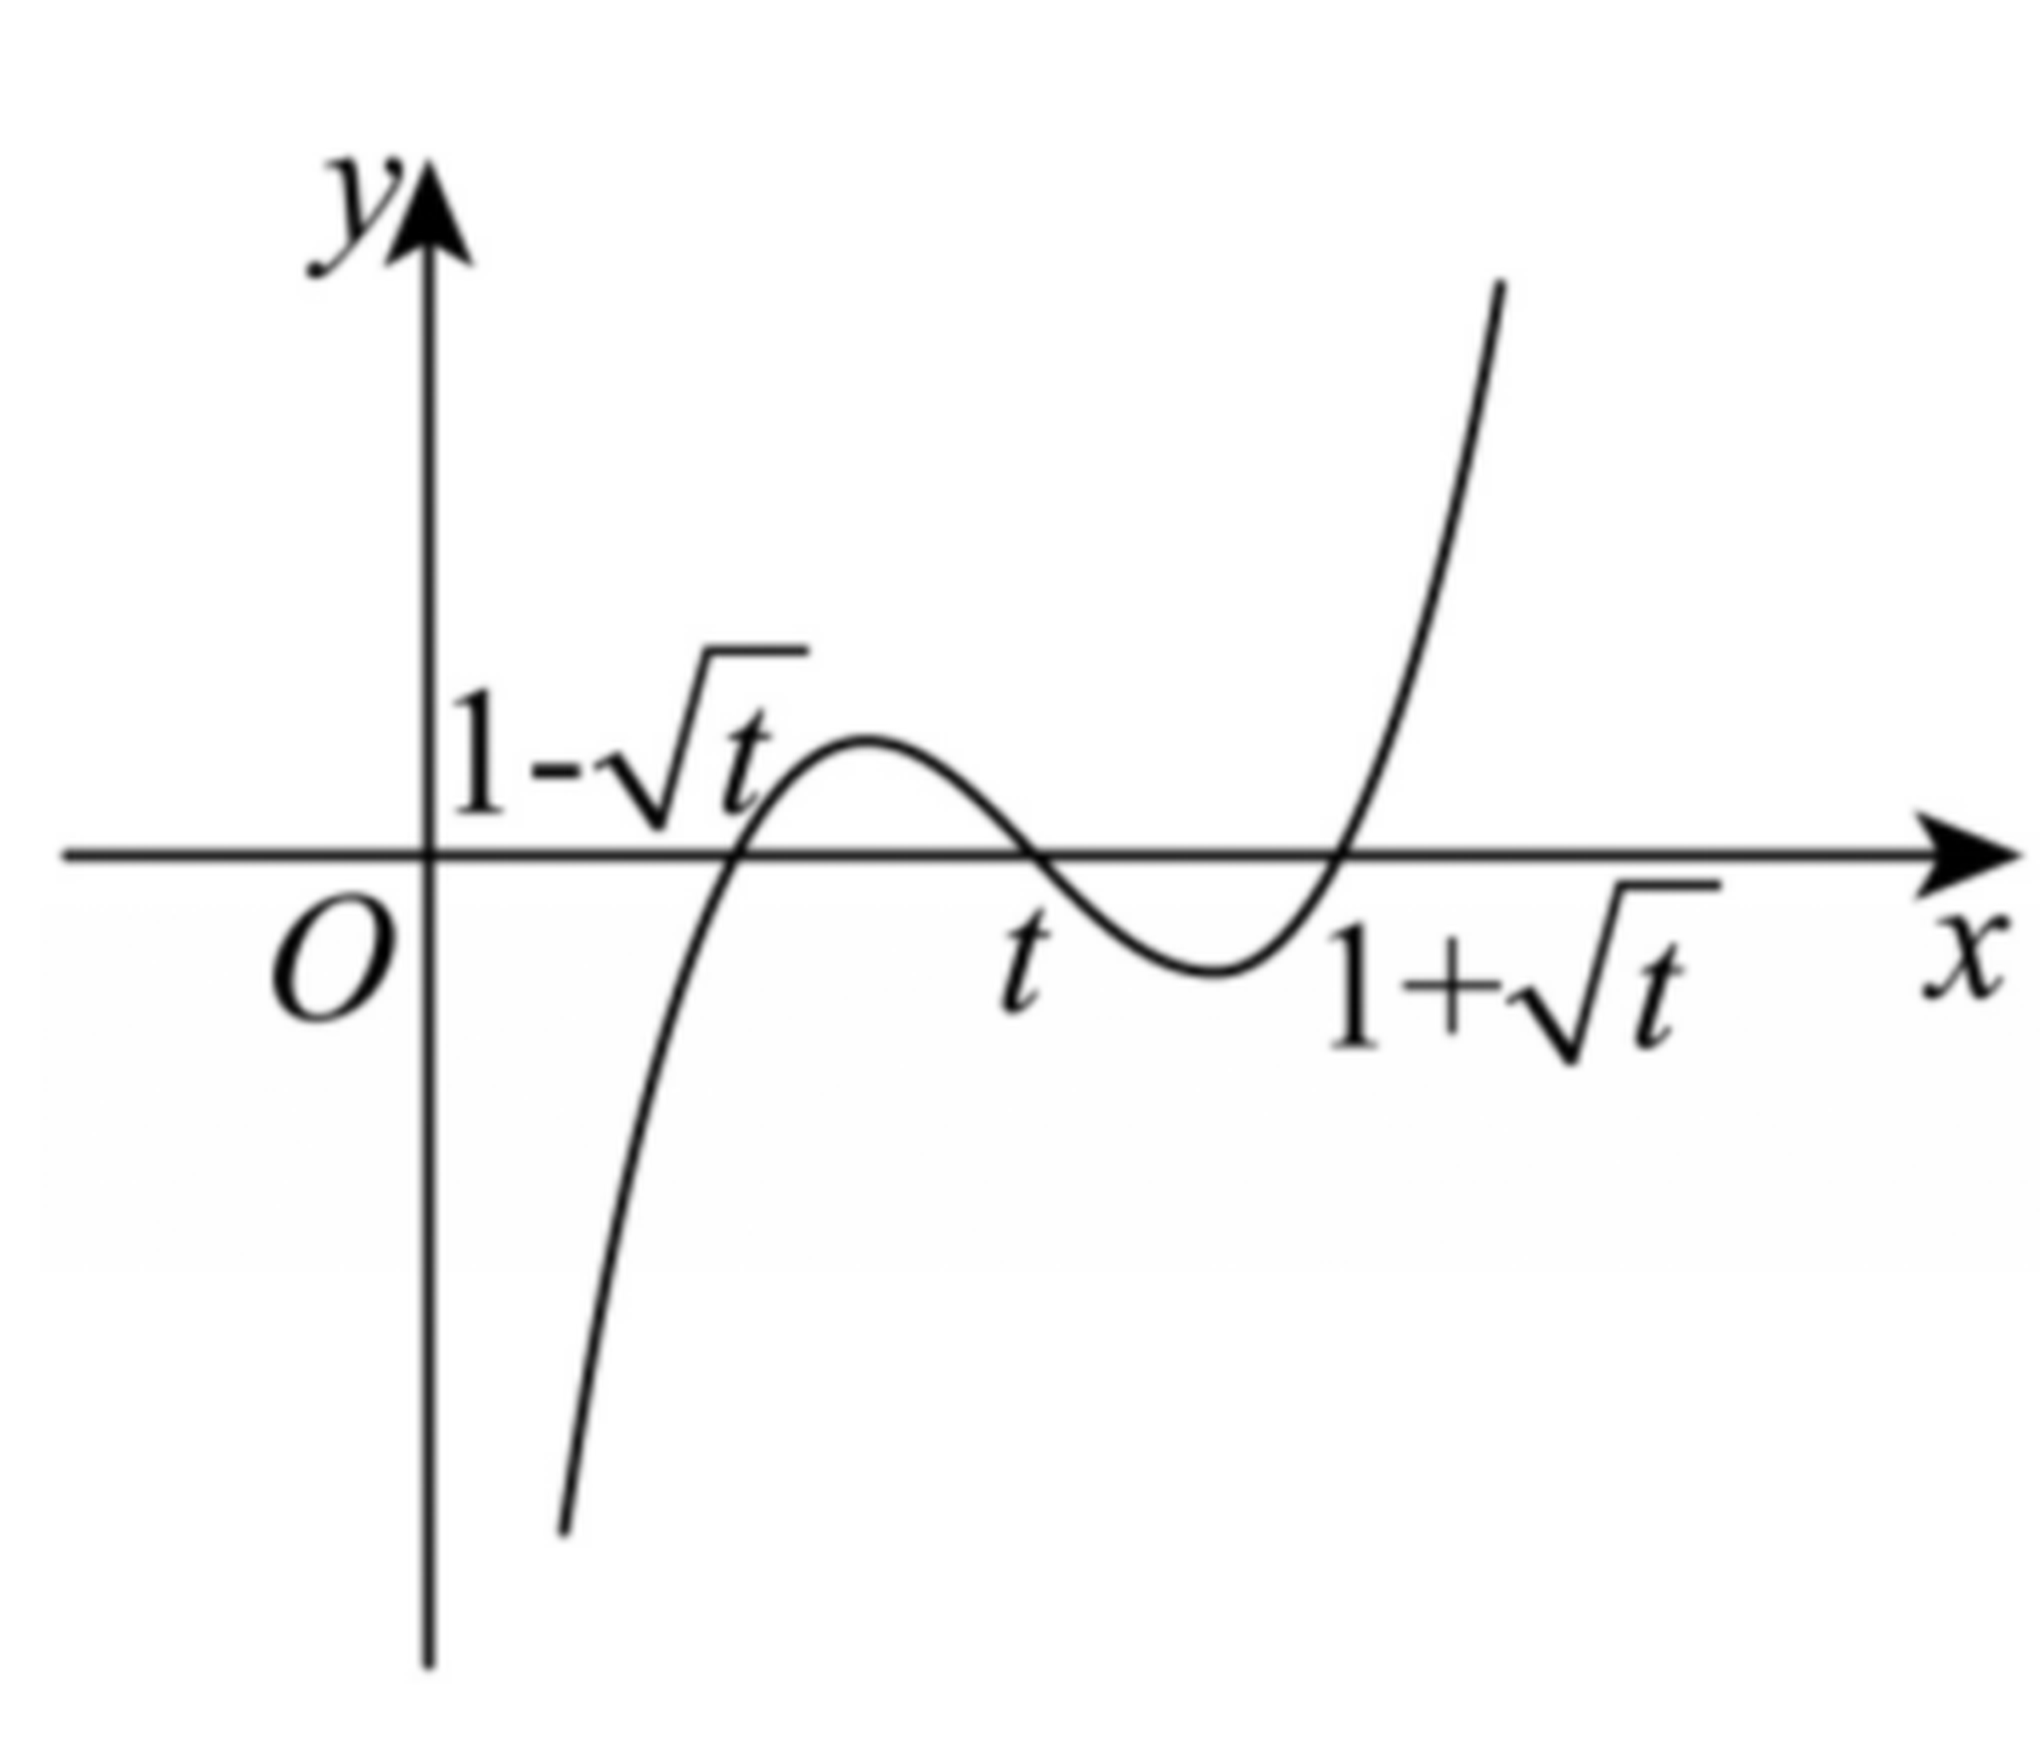
\includegraphics[width=0.40\textwidth]{figures/gao149_q12_c.png}
\end{center}
\step{则原不等式的解集为 $(-\infty,1-\sqrt t]\cup[t,1+\sqrt t]$，}
\step{当 $\begin{cases}1-\sqrt t>0\\1-\sqrt t\geqslant m\end{cases}$ 时，原不等式恒成立，此时 $t\in\left(\dfrac{3-\sqrt5}{2},1\right)$，$m\in\left(0,\dfrac{3-\sqrt5}{2}\right)$；}
\step{若 $t\geqslant1+\sqrt t$，即 $t\geqslant\dfrac{3+\sqrt5}{2}$，则取 $x=0$，$(t-1)t>0$，}
\step{原不等式不恒成立，不符合题意，}
\step{因此实数 $m$ 的取值范围是 $\left(0,\dfrac{\sqrt5+1}{2}\right]$，$m$ 的最大值是 $\dfrac{\sqrt5+1}{2}$.}
\solend
\fi

\end{enumerate}

\bigsec{二、选择题}

\begin{enumerate}
\setcounter{enumi}{12}

% === Q13 ===：答案"C"直接印在题干括号内、无【答案】/【解析】段，按 高一84 Q13／高一148 Q13 成例括号留空、另提 \ans{$C$}；四选项两行两列照原卷分行
\item 设 $ab>0$，则 $a>b$ 是 $\dfrac{1}{a}<\dfrac{1}{b}$ 的\mbox{（\quad）}

\keepwithprev
A. 充分不必要条件\qquad\qquad B. 必要不充分条件

C. 充要条件\qquad\qquad D. 既不充分又不必要条件

\ifanswer
\ans{$C$}
\fi

% === Q14 ===：$A\subset B$ 单线照录；四选项补集照原卷上划线 \overline{A}／\overline{B}；解析 1 行（由韦恩图得 B 对）
\item 已知集合 $A$、$B$ 非空，且 $A\subset B$，则下列式子中一定是空集的为\mbox{（\quad）}

\keepwithprev
A. $\overline{A}\cap B$\qquad B. $A\cap\overline{B}$\qquad C. $\overline{A}\cap\overline{B}$\qquad D. $\overline{A}\cup\overline{B}$

\ifanswer
\solbegin
\step{由韦恩图得 $B$ 对. 故选 $B$.}
\solend
\fi

% === Q15 ===："天文数字"弯引号照录；解析 2 行（首行在 04 页末、末行续 05 页顶）
\item 历史上数学计算方面的三大发明是阿拉伯数字、十进制和对数，其中对数的发明，大大缩短了计算时间，为人类研究科学和了解自然起了重大作用，对数运算对估算“天文数字”具有独特的优势. $2.5^{1000}$ 的估算值约为\mbox{（\quad）}

\keepwithprev
A. $10^{365}$\qquad B. $10^{379}$\qquad C. $10^{389}$\qquad D. $10^{398}$

\ifanswer
\solbegin
\step{$\lg 2.5^{1000}=1000\lg 2.5=1000(1-2\lg 2)\approx1000\times(1-0.602)=398$，}
\step{所以 $2.5^{1000}\approx10^{398}$. 故选 $D$.}
\solend
\fi

% === Q16 ===："完美集"新定义、圈数字①②文本模式；题干"若对任意 $x$，$y\in A$"用全角逗号、解析用顿号"$x$、$y\in A$"，两处照录不统一；解析 9 行
\item 设全集 $U=\R$，集合 $A$ 是一个非空数集，若对任意 $x$，$y\in A$，都有 $x+y\in A$、$xy\in A$，则称集合 $A$ 为一个“完美集”，给出以下命题：

①若 $A_1$、$A_2$ 都是“完美集”，且 $A_1\cap A_2\ne\varnothing$，则 $A_1\cap A_2$ 也是“完美集”；

②若 $A_1$、$A_2$ 都是“完美集”，则 $A_1\cup A_2$ 也是“完美集”.

下列说法正确的是\mbox{（\quad）}

\keepwithprev
A. ①②都是真命题\qquad\qquad B. ①是真命题，②是假命题

C. ①是假命题，②是真命题\qquad\qquad D. ①②都是假命题

\ifanswer
\solbegin
\step{由题意，全集 $U=\R$，集合 $A$ 是一个非空数集，}
\step{若对任意 $x$、$y\in A$，都有 $x+y\in A$、$xy\in A$，则称集合 $A$ 为一个“完美集”，}
\step{对于①，取 $x$、$y\in A_1\cap A_2$，则 $x\in A_1$，$x\in A_2$，$y\in A_1$，$y\in A_2$，}
\step{又 $A_1$、$A_2$ 是“完美集”，所以 $x+y\in A_1$，$xy\in A_1$，$x+y\in A_2$，$xy\in A_2$，}
\step{所以 $x+y\in A_1\cap A_2$，$xy\in A_1\cap A_2$，所以 $A_1\cap A_2$ 是“完美集”，故①正确；}
\step{对于②，取“完美集” $A_1=\{x\mid x=2k,k\in\Z\}$，$A_2=\{x\mid x=3k,k\in\Z\}$，}
\step{则 $2\in A_1$，$3\in A_2$，但 $2+3\notin A_1\cup A_2$，}
\step{即此时 $A_1\cup A_2$ 不是“完美集”，故②错误.}
\step{故选 $B$.}
\solend
\fi
\end{enumerate}

\bigsec{三、解答题}

\begin{enumerate}
\setcounter{enumi}{16}

% === Q17 ===："图像"（有亻）照录（Q17 题干与解析共 2 处）；绝对值 \lvert…\rvert；解析 7 行
\item 已知 $m\in\R$，$f(x)=(m^2-m-5)x^m$. 若 $y=f(x)$ 是幂函数，且其图像不经过原点.

(1) 求实数 $m$ 的值；

(2) 若 $f(a)=f(b)$ 且 $a\ne b$，求 $\lvert a+2\rvert+\lvert b-1\rvert$ 的最小值，并指出取到最小值时 $a$ 的取值范围.

\ifanswer
\solbegin
\step{(1) $f(x)=(m^2-m-5)x^m$ 是幂函数，得 $m^2-m-5=1$，即 $m^2-m-6=0$，}
\step{解得 $m=-2$ 或 $m=3$，又函数图像不经过原点，所以 $m=-2$($3$ 舍)；}
\step{(2) 由 (1) 得 $f(x)=x^{-2}=\dfrac{1}{x^2}$ 为偶函数，}
\step{$x<0$ 时，函数 $f(x)$ 严格增，$x>0$ 时，函数 $f(x)$ 严格减，}
\step{又 $f(a)=f(b)$ 且 $a\ne b$，所以 $a=-b$，且 $a\ne0$，$b\ne0$，}
\step{则 $\lvert a+2\rvert+\lvert b-1\rvert=\lvert a+2\rvert+\lvert-a-1\rvert=\lvert a+2\rvert+\lvert a+1\rvert$，}
\step{则 $\lvert a+2\rvert+\lvert b-1\rvert$ 的最小值为 $1$，取到最小值时 $a$ 的取值范围是 $[-2,-1]$.}
\solend
\fi

% === Q18 ===：判别式两形混用——(1) cases 块印高 \Delta、(2) 独立行印扁 \triangle，逐处照录不统一；解析 8 行
\item 已知命题 $p$：方程 $x^2+4x+m-1=0$ 有两个不等的负根；命题 $q$：方程 $4x^2+4x+m-2=0$ 无实根.

(1) 若 $p$ 为真命题，求 $m$ 的取值范围；

(2) 若 $p$、$q$ 两命题一真一假，求 $m$ 的取值范围.

\ifanswer
\solbegin
\step{(1) 若 $p$ 为真命题，即方程 $x^2+4x+m-1=0$ 有两个不等的负根；}
\step{必有 $\begin{cases}\Delta=16-4(m-1)>0\\m-1>0\end{cases}$，解得 $1<m<5$，即 $m$ 的取值范围为 $(1,5)$；}
\step{(2) 命题 $q$：方程 $4x^2+4x+m-2=0$ 无实根，}
\step{则有 $\triangle=16-16(m-2)<0$，解得 $m>3$，}
\step{若 $p$ 和 $q$ 有且只有一个为真命题，}
\step{若 $p$ 真 $q$ 假，必有 $\begin{cases}1<m<5\\m\leqslant3\end{cases}$，则有 $1<m\leqslant3$，}
\step{若 $p$ 假 $q$ 真，必有 $\begin{cases}m\leqslant1\text{ 或 }m\geqslant5\\m>3\end{cases}$，则有 $m\geqslant5$，}
\step{综上，$1<m\leqslant3$ 或 $m\geqslant5$.}
\solend
\fi

% === Q19 ===：$A\subseteq B$ 带下划线照录；解析 7 行（(2) 两组 cases 并排）
\item 已知 $m\in\R$，集合 $A=\left\{x\mid y=\sqrt{3-x}-\dfrac{1}{\sqrt{x-1}}\right\}$，集合 $B=\{x\mid 2m\leqslant x\leqslant1-m\}$.

(1) 若 $A\cup B=B$，求实数 $m$ 的取值范围；

(2) 若 $A\cap B=\varnothing$，求实数 $m$ 的取值范围.

\ifanswer
\solbegin
\step{(1) 函数 $y=\sqrt{3-x}-\dfrac{1}{\sqrt{x-1}}$，则 $\begin{cases}3-x\geqslant0\\x-1>0\end{cases}$，解得 $1<x\leqslant3$，}
\step{所以 $A=\{x\mid1<x\leqslant3\}$，}
\step{因为 $A\cup B=B$，所以 $A\subseteq B$，则 $\begin{cases}2m\leqslant1\\1-m\geqslant3\end{cases}$，解得 $m\leqslant-2$，}
\step{综上，实数 $m$ 的取值范围为 $(-\infty,-2]$；}
\step{(2) 当 $B=\varnothing$ 时，则 $2m>1-m$，解得 $m>\dfrac{1}{3}$，}
\step{当 $B\ne\varnothing$ 时，则 $\begin{cases}2m\leqslant1-m\\2m>3\end{cases}$ 或 $\begin{cases}2m\leqslant1-m\\1-m\leqslant1\end{cases}$，解得 $m\in\varnothing$ 或 $0\leqslant m\leqslant\dfrac{1}{3}$，}
\step{综上，实数 $m$ 的取值范围为 $[0,+\infty)$.}
\solend
\fi

% === Q20 ===：n 阶基本不等式推广；(3) 解析含 \overbrace{…}^{k} 上括号；(2) 解析"x=x=x=3(1-x)"三连等系原卷笔误、照录加注（见 ⑤）；解析 14 行
\item 教材中的基本不等式可以推广到 $n$ 阶：$n$ 个正数的算术平均数不小于它们的几何平均数，即对于任意的正数 $a_1$、$a_2$、$\cdots$、$a_n$，有 $\dfrac{a_1+a_2+\cdots+a_n}{n}\geqslant\sqrt[n]{a_1\cdot a_2\cdots a_n}$（$n\in\N$ 且 $n\geqslant2$），且等号当且仅当 $a_1=a_2=\cdots=a_n$ 时成立. 利用此结论解决下列问题：

(1) 若 $x$、$y$、$z>0$，求 $\dfrac{y}{x}+\dfrac{2z}{y}+\dfrac{4x}{z}$ 的最小值；

(2) 已知 $0<x<1$，求 $x^3(1-x)$ 的最大值，并求取得最大值时的 $x$ 的值；

(3) 对任意的正整数 $k$，判断 $\left(1+\dfrac{1}{k}\right)^k$ 与 $\left(1+\dfrac{1}{k+1}\right)^{k+1}$ 的大小关系，并证明.

\ifanswer
\solbegin
\step{(1) 因为 $x$、$y$、$z>0$，有 $\dfrac{y}{x}>0$，$\dfrac{2z}{y}>0$，$\dfrac{4x}{z}>0$}
\step{所以 $\dfrac{y}{x}+\dfrac{2z}{y}+\dfrac{4x}{z}\geqslant3\sqrt[3]{\dfrac{y}{x}\cdot\dfrac{2z}{y}\cdot\dfrac{4x}{z}}=3\sqrt[3]{8}=6$，}
\step{当且仅当 $\dfrac{y}{x}=\dfrac{2z}{y}=\dfrac{4x}{z}$ 时取等号，故 $\dfrac{y}{x}+\dfrac{2z}{y}+\dfrac{4x}{z}$ 的最小值为 $6$.}
\step{(2) 因为 $0<x<1$，所以 $1-x>0$，}
\step{$x^3(1-x)=\dfrac{1}{3}[x\cdot x\cdot x\cdot3(1-x)]\leqslant\dfrac{1}{3}\left[\dfrac{x+x+x+3(1-x)}{4}\right]^4=\dfrac{1}{3}\times\left(\dfrac{3}{4}\right)^4$}
\step{$=\dfrac{27}{256}$，当且仅当 $x=x=x=3(1-x)$，即 $x=3(1-x)$，$x=\dfrac{3}{4}$ 取等号，}% 原卷"x=x=x=3(1-x)"三连等，疑为四因子相等之误排，放大 08 页确认，照录未改（见 ⑤）
\step{所以 $0<x<1$ 时，$x^3(1-x)$ 的最大值是 $\dfrac{27}{256}$，取最大值时 $x=\dfrac{3}{4}$.}
\step{(3) 对任意 $k\in\N^*$，$\left(1+\dfrac{1}{k}\right)^k<\left(1+\dfrac{1}{k+1}\right)^{k+1}$.}
\step{证明：$\left(1+\dfrac{1}{k}\right)^k=\overbrace{\left(1+\dfrac{1}{k}\right)\cdot\left(1+\dfrac{1}{k}\right)\cdots\left(1+\dfrac{1}{k}\right)}^{k}\times1$}
\step{$\leqslant\left(\dfrac{\overbrace{\left(1+\dfrac{1}{k}\right)+\left(1+\dfrac{1}{k}\right)+\cdots+\left(1+\dfrac{1}{k}\right)}^{k}+1}{k+1}\right)^{k+1}$}
\step{$=\left(\dfrac{\overbrace{(1+1+\cdots+1)}^{k}+\overbrace{\left(\dfrac{1}{k}+\dfrac{1}{k}+\cdots+\dfrac{1}{k}\right)}^{k}+1}{k+1}\right)^{k+1}=\left(\dfrac{k+1+1}{k+1}\right)^{k+1}=\left(1+\dfrac{1}{k+1}\right)^{k+1}$，}
\step{当且仅当 $1+\dfrac{1}{k}=1$ 时取等号，}
\step{但是任意 $k\in\N^*$ 时 $1+\dfrac{1}{k}>1$，所以等号不成立，}
\step{故任意 $k\in\N^*$ 时，$\left(1+\dfrac{1}{k}\right)^k<\left(1+\dfrac{1}{k+1}\right)^{k+1}$.}
\solend
\fi

% === Q21 ===："减 k 集"新定义（引号内 k／数字两侧空格照录）；解析 26 行（续 10 页），含 ⑤ 三处原卷笔误照录
\item 定义：对于给定的整数 $k$，若非空集合 $A$ 满足如下 3 个条件：

① $A$ 是正整数集的子集；② $A\ne\{1\}$；

③对任意正整数 $x,y$，若 $x+y\in A$，则 $xy-k\in A$；则称集合 $A$ 为“减 $k$ 集”.

(1) 判断集合 $A=\{1,2\}$ 是否为“减 $0$ 集”？是否为“减 $1$ 集”？（无需说明理由）

(2) 证明：不存在“减 $2$ 集”；

(3) 是否存在“减 $1$ 集”？如果存在，求出所有“减 $1$ 集”；如果不存在，说明理由.

\ifanswer
\solbegin
\step{(1) 因为 $P\subseteq\N^*$，$P\ne\{1\}$，$1+1=2\in P$，$1\times1-0\in P$，}
\step{所以集合 $P=\{1,2\}$ 是“减 $0$ 集”；}
\step{因为 $P\subseteq\N^*$，$P\ne\{1\}$，$1+1=2\in P$，$1\times1-1\notin P$，}
\step{所以集合 $P=\{1,2\}$ 是“减 $1$ 集”；}% 按条件③应为"不是"，原卷径印"是"，放大 09 页确认，照录未改（见 ⑤）
\step{(2) 假设存在集合 $A$ 是“减 $2$ 集”，若 $x+y\in A$，则 $xy-2\in A$，}
\step{①当 $x+y=xy-2$ 时，有 $(x-1)(y-1)=3$，}
\step{则 $x$、$y$ 一个为 $2$，一个为 $4$，所以集合 $A$ 有元素 $6$，}
\step{但 $3+3\in A$，$3\times3-2\notin A$，与 $A$ 是“减 $2$ 集”矛盾；}
\step{②当 $x+y\ne xy-2$ 时，则 $x+y=xy-1$ 或 $x+y=xy-m$($m>2$)，}
\step{若 $x+y=xy-1$，$m=1$ 时，$M$ 为除 $1$ 以外的最小元素，}% 原卷"m=1"上文未显式定义，疑笔误，放大 09 页确认，照录未改（见 ⑤）
\step{则 $x=M-1$，$y=1$ 时，$xy-2=M-3$ 小于 $M$，}
\step{要符合题意，必须 $M=4$，}
\step{此时取 $x-2$，$y=2$，$xy-2=2$ 不属于 $A$，故不符合题意，}% 原卷"取 x−2"疑为"取 x=2"误排，放大 09 页确认，照录未改（见 ⑤）
\step{当 $m>2$ 时，$(x-1)(y-1)=m+1$，同样得出矛盾，}
\step{综上，不存在 $A$ 是“减 $2$ 集”.}
\step{(3) 存在“减 $1$ 集” $A$，则 $A\ne\{1\}$，}
\step{①假设 $1\in A$，则 $A$ 中除了元素 $1$ 以外，必然还含有其它元素，}
\step{假设 $2\in A$，$1+1\in A$，而 $1\times1-1\notin A$，所以 $2\notin A$，}
\step{假设 $3\in A$，$1+2\in A$，而 $1\times2-1\in A$，所以 $3\in A$，}
\step{所以 $A=\{1,3\}$，}
\step{假设 $4\in A$，$1+3\in A$，而 $1\times3-1\notin A$，所以 $4\notin A$，}
\step{假设 $5\in A$，$1+4\in A$，$1\times4-1\in A$，$2+3=5$，$2\times3-1\in A$，所以 $5\in A$，}
\step{所以 $A=\{1,3,5\}$，}
\step{以此类推，得 $A=\{1,3,5,\cdots,2n-1,\cdots\}$，($n\in\N^*$)，}
\step{所以所有的“减 $1$ 集”有 $\{1,3\}$，$\{1,3,5\}$，$\{1,3,5,7\}$，$\cdots$，$\{1,3,5,\cdots,2n-1,\cdots\}$，}
\step{$(n\in\N^*)$.}
\solend
\fi
\end{enumerate}

\end{document}
"
% 紧凑版：xelatex "\def\iscompact{1}% 高一149_青浦高级中学上外云间_期中.tex
%   —— 高一上数学"2026-2027 年青浦高级中学上外云间高一上期中"（试卷版/答案版/紧凑版）
% 试卷版：xelatex 高一149_青浦高级中学上外云间_期中.tex
% 答案版：xelatex "\def\isanswer{1}% 高一149_青浦高级中学上外云间_期中.tex
%   —— 高一上数学"2026-2027 年青浦高级中学上外云间高一上期中"（试卷版/答案版/紧凑版）
% 试卷版：xelatex 高一149_青浦高级中学上外云间_期中.tex
% 答案版：xelatex "\def\isanswer{1}\input{高一149_青浦高级中学上外云间_期中.tex}"
% 紧凑版：xelatex "\def\iscompact{1}\input{高一149_青浦高级中学上外云间_期中.tex}"
%
% ① 原始材料：微信公众号"魔都数学加油站"文章，连载"27学年高一149"，原文标题
% "27学年高一149——2026-2027年上海市青浦高级中学上外云间高一上期中"；
% 原文链接：https://mp.weixin.qq.com/s/T7_nyoR1k0o_5og7FkDsyw 。
% 正文为 10 张 PNG 页（01/02/03/04/10 为 2560×3620，05/06/07/08/09 为 4762×6735，
% 同一篇各页分辨率混排，逐页按各自分辨率裁图核对，别按预览比例换算裁框）。
% 体例：混合体例讲评版——19 题中 Q6 只印【答案】、无【解析】；Q13 的答案"C"
%   直接印在题干括号内、无【答案】/【解析】段；其余 17 题印【解析】（逐题核实，见 ② ②）。
% 题目、答案、解析均据原图转录；卷面粉红色水印"魔都数学加油站"及公众号页脚未录入。
% 全卷插图清单（逐页通读 10 页确认）：1 幅题目配图 + 3 幅【解析】内配图：
%   · Q11 矩形 ABCD 折叠几何图（02 页右侧：A/B/C/D/E/F/C' 与虚线 EB、BC、FC），
%     题干"如图"处，题目配图、三版都出，裁 figures/gao149_q11.png；
%   · Q12【解析】内 3 幅三次函数曲线坐标图（03 页右侧两幅 + 04 页右侧一幅：
%     x/y 轴、O、t、1-\sqrt t、1+\sqrt t 等标注，分别对应 t<1-\sqrt t、
%     t=1-\sqrt t、1+\sqrt t>t>1-\sqrt t 三种情形），解析配图、仅答案版出，
%     分别裁 figures/gao149_q12_a.png／_b.png／_c.png，放 \ifanswer 内 \step 之间
%     （高一73 第 16 题成例）；
%   其余各页逐页确认无其它题目配图、无表格；Q14 解析"由韦恩图得 B 对"仅文字推导、
%   原卷并未印韦恩图；Q9／Q18／Q19 的 cases 块与 Q20(3) 的 \overbrace 为数学块（非图）；
%   10 页下半仅水印、无正文。4 图均取自原卷截图，去粉色水印、去色、4× LANCZOS 放大。
%
% 卷首标题：原卷印作"2026-2027 年青浦高级中学上外云间高一上期中"，年份区间按全稿
% 惯例排 en dash；原卷卷面未印副标题，本稿按同期中卷（高一140／141／143／144／145／
% 146／147／148）知识模块口径补出"集合与常用逻辑用语、不等式、函数"。
%
% 题号体例（逐页核实定稿）：本卷共 19 题——一、填空题 3—12（10 题）、
% 二、选择题 13—16（4 题）、三、解答题 17—21（5 题）。
% 三节分别 \setcounter{enumi}{2}／{12}／{16}。原卷从第 3 题起、无第 1、2 题，
% 本稿保留原题号；全卷无附加题节（Q21 解析末行"（n\in N^*）."为全卷收尾）。
%
% ② 与原卷的排版差异：
%   ① 原文从第 3 题起，本稿保留原题号；共 19 题三节；
%   ② 混合体例逐题核实：Q6（反证法"假设的内容"）只印【答案】、无【解析】，
%      按 高一140 第 5 题／高一145 Q3 成例提 \ans{}、不补造解析；Q13 答案"C"直接
%      印在题干括号内、全卷无该题【答案】/【解析】段，按 高一84 Q13／高一148 Q13
%      成例括号 \mbox{（\quad）} 留空、另提 \ans{$C$}；其余 17 题印【解析】、
%      用 \solbegin…\solend，选择题答案在解析末句"故选 X"（Q14 选 B、Q15 选 D、
%      Q16 选 B，逐个放大 04/05 页核实）、题干括号留空、不另提 \ans{}；
%      答案版【答案】/【解析】标记数 = 19（2 个 \ans ＋ 17 个 \solbegin）
%      = 全卷题数；
%   ③ 原卷卷面未印副标题，本稿按知识模块口径补出；
%   ④ 原卷填空横线按全稿惯例排 \blankline[4.4em]；选择题括号排 \mbox{（\quad）}、
%      选项段前按惯例加 \keepwithprev；Q13／Q16 四选项为两行两列、Q14／Q15
%      选项为一行，照原卷分行；解答题不留作答区、不加 \anspace（原卷为讲评版）；
%   ⑤ 数集：Q6"a,b\in N"、Q8"x\in R"、Q9"a\in R"／"解集为 R"、Q12"t\in R"、
%      Q16"U=R"、Q17"m\in R"、Q19"m\in R"、Q20"n\in N" 原卷印斜体 R/N，
%      按全稿惯例统一改 \R／\N；Q20(3)、Q21 的 $N^*$ 排 \N^*；Q16 解析
%      "$k\in Z$" 排 \Z。绝对值排 \lvert…\rvert（Q17），集合描述竖线排 \mid
%      （Q19、Q16 解析）；不等号按全稿惯例排 \leqslant／\geqslant；
%      补集照原卷上划线排 \overline{A}／\overline{B}（Q14 四选项）；空集
%      \varnothing（Q16、Q19、Q21）；
%   ⑥ 子集符号逐处照录不统一：Q4 题干"{1,2}⊆A⊂{1,2,3,4,5,6}" 前者印带下划线
%      ⊆、照录 \subseteq，后者印单线 ⊂、照录 \subset；Q10"A⊆{-1,1/2,2,3}"、
%      Q19 解析"A⊆B"、Q21 解析"P⊆N*" 均印带下划线 ⊆、照录 \subseteq；
%      Q14"A⊂B" 印单线 ⊂、照录 \subset（逐处放大 01/02/04/07/09 页确认，见 ④）；
%   ⑦ 子题标号 (1)(2)(3) 半角括号照录；圈数字 ①②③ 在文本模式（Q16 两命题、
%      Q21 三个条件与解析的①②）按 common.sty 划入 CJK 字符类渲染；cases 块整体
%      算一个印刷行；\left…\right 不得拆到不同 $…$ 组；数学式内 CJK 用 \text{}
%      （Q18 解析 cases 块"\text{或}"）；Q11 解析"Rt\triangle DC'F" 的 Rt 照录；
%   ⑧ 题干／解析中的中文弯引号按原卷照录：Q6" 已知 a,b\in N，若 ab 能被 5 整除，
%      那么 a、b 中至少有一个能被 5 整除 "（开引号后紧跟"已知"、闭引号后空格接"时"）、
%      Q15"天文数字"、Q16"完美集"、Q21"减 k 集""减 0 集""减 1 集""减 2 集"
%      （引号内 k／数字两侧有空格），注释内一律 ASCII 引号；
%   ⑨ 半角逗号在数学组之间是全稿惯例、非笔误（Q8"$a>0,a\ne1,x\in\R$"、
%      Q21 题干"$x,y$" 等），逐处照录别改；Q16 题干"若对任意 $x$，$y\in A$"
%      用全角逗号而解析用顿号"$x$、$y\in A$"，两处不同均照录；行末西文句点
%      照录为 ASCII `.`；行中全角逗号／顿号照录；
%   ⑩ "图像／图象"逐处放大核：Q10 题干与解析共 6 处均印"图象"（象，无亻）；
%      Q17 题干"其图像不经过原点"与解析"又函数图像不经过原点" 2 处印"图像"
%      （像，有亻），逐处照录未统一改动（放大 02/05/06 页确认）；
%   ⑪ 判别式 Δ/△ 混用是照录项：Q9 解析 cases 块"Δ=4(a−2)²+16(a−2)<0"、
%      Q18(1) cases 块"Δ=16−4(m−1)>0" 两处印等腰偏高粗三角 \Delta；
%      Q18(2) 独立行"△=16−16(m−2)<0" 印扁等边细线三角 \triangle，
%      逐处放大判断、照录不统一（参照 高一142／144／145／146／148 头注④口径）；
%      另 Q11 题干"△C'DF 面积"与解析 3 处"△"（含"Rt△DC'F"）共 4 处几何
%      三角形符号亦印扁细线三角，照录 \triangle（非判别式，字形同类，见 ④）；
%   ⑫ 一条 \step = 原卷解析的一个印刷行，cases 块整体算一个印刷行；别把原卷折行
%      并起来、别把一行拆多条。Q11 十三行（7 行在 02 页＋6 行在 03 页）、
%      Q12 十五行（8 行在 03 页＋7 行在 04 页）、Q16 九行、Q21 二十六行
%      （续 10 页）均按印刷行逐条断，不丢行；
%   ⑬ 配图：Q11 题目配图（三版都出）放 \item 内题干之后 \begin{center}，
%      大图块加 \needvspace{8cm} 守卫把整块推走（守卫放 \item 之前，见
%      高一145 Q14/Q20 成例与切页审计 B 类坑）；Q12 三幅解析配图（仅答案版出）
%      放 \ifanswer 内 \solbegin…\solend 的 \step 之间；三版切页审计均"合计异常：无"；
%   ⑭ 跨页续印按题合并：Q3/4/5 在 01 页；Q6/7/8 题干与解析在 01 页；
%      Q9 题干在 01 页末、解析 4 行在 02 页顶；Q10 题干＋解析在 02 页；
%      Q11 题干＋图＋解析前 7 行在 02 页、解析后 6 行续 03 页顶；
%      Q12 题干＋解析首行在 03 页末、解析续 7 行在 03 页下半＋7 行在 04 页顶，
%      "二、选择题"标题在 04 页下半；Q13/14 题干＋选项＋Q14 解析在 04 页下半；
%      Q15 题干＋选项＋解析首行在 04 页末、末行"所以 2.5^1000≈10^398. 故选 D."
%      续 05 页顶；Q16 题干＋选项＋解析 9 行在 05 页、"三、解答题"标题＋
%      Q17 题干首句在 05 页末；Q17(2)＋解析 7 行、Q18 题干＋解析前 6 行在 06 页；
%      Q18 解析末 2 行续 07 页顶；Q19 题干＋解析 4 行在 07 页上半、
%      解析续 3 行在 07 页下半；Q20 题干(1) 在 07 页末、题干(2)(3)＋解析(1)(2)
%      在 08 页上半、(3) 解析含 \overbrace 的证明在 08 页下半、末行
%      "故任意 k∈N* 时…"续 09 页顶；Q21 题干＋解析(1)(2)(3) 前段在 09 页、
%      解析(3) 后半 9 行续 10 页上半（10 页下半仅水印、无正文）。
%      本稿按题连排，不丢行、不并折行；
%   ⑮ 原卷解析内无红色"法一／法二"之类小标题，故本卷无 \stepm；水印
%      "魔都数学加油站"红色不录入。
%
% ③ 行数复核：一条 \step／\stepm = 原卷解析的一个印刷行，cases 块作一个印刷行计。
%   逐题数（主会话逐页核对定稿）：Q3：1；Q4：2；Q5：2；Q6：0（只印【答案】、
%   提 \ans{}）；Q7：1；Q8：1；Q9：4；Q10：5；Q11：13；Q12：15；
%   Q13：0（答案印在题干括号内、另提 \ans{}）；Q14：1；Q15：2；Q16：9；
%   Q17：7；Q18：8；Q19：7；Q20：14；Q21：26。
%   合计 118 条 \step（本卷无 \stepm：解析内无红色"法一／法二"类小标题），
%   与原卷逐题印刷行相等。全卷 17 题设 \solbegin…\solend ＋ 2 处 \ans{}，
%   答案版【答案】/【解析】标记数 = 19 = 全卷题数。
%
% ④ 判别式／子集符号结论（逐处放大原图照录、不得统一，主会话像素级复核）：
%   判别式全卷 3 处，两形混用逐处照录不统一（参照 高一142／144／145／146／148 头注④）：
%     · Q9 解析 cases 块"Δ=4(a−2)²+16(a−2)<0" 原卷印等腰偏高粗三角（高>宽、
%       粗笔画），照录 \Delta（放大 02 页 /tmp/gao149/z/t02_q9_delta2.png 确认）；
%     · Q18(1) cases 块"Δ=16−4(m−1)>0" 原卷印等腰偏高粗三角（高>宽、粗笔画），
%       照录 \Delta（放大 06 页 /tmp/gao149/z/t06_q18a.png 确认）；
%     · Q18(2) 独立行"△=16−16(m−2)<0" 原卷印扁等边细线三角（宽>高、细线），
%       照录 \triangle（放大 06 页 /tmp/gao149/z/t06_q18b.png 与 Q18(1) 并排确认）。
%   另 Q11 题干"△C'DF"与解析 3 处"△"（含"Rt△DC'F"）共 4 处几何三角形符号
%     亦印扁等边细线三角，照录 \triangle（放大 02 页
%     /tmp/gao149/z/t02_q11_tri2.png 确认），与 Q9／Q18(1) 判别式 \Delta 两形不统一。
%   子集／补集：Q4 题干"{1,2}⊆A⊂{1,2,3,4,5,6}" 前者带下划线 ⊆、照录 \subseteq，
%     后者单线 ⊂、照录 \subset（放大 01 页 /tmp/gao149/z/t01_q3q4.png 确认）；
%     Q10"A⊆{-1,1/2,2,3}"、Q19 解析"A⊆B"、Q21 解析"P⊆N*" 三处带下划线 ⊆、
%     照录 \subseteq；Q14"A⊂B" 单线 ⊂、照录 \subset（放大 04 页
%     /tmp/gao149/z/t04_q14_sub2.png 确认）；Q14 四选项补集 \overline{A}／\overline{B}
%     照原卷上划线；空集 \varnothing（Q16、Q19、Q21）；Q19／Q16 解析集合描述竖线
%     \mid；数集 \R／\N／\N^*／\Z 归一见 ② ⑤。
%
% ⑤ 存疑照录（放大原图确认，照录未改、正文对应处另有 % 注）：
%   1. Q21 解析(1) 第二组"因为 P⊆N*，P≠{1}，1+1=2∈P，1×1−1∉P，所以集合
%      P={1,2} 是"减 1 集"" —— 按条件③（x=y=1 时 xy−1=0 须∈P）应为"不是"，
%      原卷却径印"是"，放大 09 页 /tmp/gao149/z/t09_q21_sol1.png 确认，照录未改
%      （疑为原卷结论笔误）。
%   2. Q21 解析(2)"此时取 x−2，y=2，xy−2=2 不属于 A" —— 按上下文应为
%      "取 x=2"（x−2 疑为 x=2 的误排），放大 09 页
%      /tmp/gao149/z/t09_q21_sol2.png 确认，照录未改。
%   3. Q21 解析(2)"若 x+y=xy−1，m=1 时，M 为除 1 以外的最小元素" 中 $m=1$
%      上文未显式定义 m（仅"x+y=xy−m(m>2)"中出现），放大 09 页确认，照录未改。
%   4. Q20 解析(2)"当且仅当 x=x=x=3(1−x)" 三个 x 连等，疑为原卷排印（应为
%      四个因子 x,x,x,3(1−x) 相等），放大 08 页
%      /tmp/gao149/z/t08_q20_sol2.png 确认，照录未改。
%   5. Q6 只印【答案】、Q13 答案印题干括号内，两题均无【解析】，按成例提
%      \ans{}、未补造解析（见 ② ②）。
%   6. 判别式 Q9／Q18(1) 高 \Delta 与 Q18(2)／Q11 扁 \triangle 两形混用，逐处
%      照录不统一（见 ④）；"图像／图象" Q10 用"图象"、Q17 用"图像"，
%      逐处照录未统一（见 ② ⑩）。
%   全卷除此 6 类外未发现其它笔误／自相矛盾处。
%
% ⑥ 跨页续印按题合并说明：见 ② ⑭。
%
\documentclass[a4paper,11pt]{article}
\usepackage{common}

\begin{document}

\examtitlest[3]{2026--2027 年青浦高级中学上外云间高一上期中}{集合与常用逻辑用语、不等式、函数}

\bigsec{一、填空题}

\begin{enumerate}
\setcounter{enumi}{2}

% === Q3 === 根式化分数指数幂；解析 1 行
\item 根式 $\sqrt{a\sqrt a}$ 化成分数指数幂是\blankline[4.4em].

\ifanswer
\solbegin
\step{$\sqrt{a\sqrt a}=\sqrt{a\cdot a^{\frac{1}{2}}}=\sqrt{a^{1+\frac{1}{2}}}=\sqrt{a^{\frac{3}{2}}}=a^{\frac{3}{2}\times\frac{1}{2}}=a^{\frac{3}{4}}$.}
\solend
\fi

% === Q4 === 题干两种子集符号逐处照录（\subseteq 带下划线／\subset 单线）；解析 2 行
\item 满足 $\{1,2\}\subseteq A\subset\{1,2,3,4,5,6\}$ 的集合 $A$ 共有\blankline[4.4em]个.

\ifanswer
\solbegin
\step{集合 $A$ 满足 $\{1,2\}\subseteq A\subset\{1,2,3,4,5,6\}$，}% 前者带下划线 $\subseteq$、后者单线 $\subset$，逐处照录不统一（放大 01 页确认）
\step{所以集合 $A$ 的个数为集合 $\{3,4,5,6\}$ 的真子集的个数，即为 $2^4-1=15$ 个.}
\solend
\fi

% === Q5 === 解析 2 行
\item 不等式 $\dfrac{2x+1}{x-1}\leqslant0$ 的解集为\blankline[4.4em].

\ifanswer
\solbegin
\step{不等式 $\dfrac{2x+1}{x-1}\leqslant0$ 可化为 $(2x+1)(x-1)\leqslant0$，且 $x-1\ne0$，解得 $-\dfrac{1}{2}\leqslant x<1$，}
\step{即原不等式的解集为 $\left[-\dfrac{1}{2},1\right)$.}
\solend
\fi

% === Q6 === 原卷只印【答案】、无【解析】，按 高一140 第 5 题／高一145 Q3 成例提 \ans{}、不补造解析；弯引号与空格照录
\item 用反证法证明命题 “已知 $a,b\in\N$，若 $ab$ 能被 5 整除，那么 $a$、$b$ 中至少有一个能被 5 整除” 时，假设的内容应该是\blankline[4.4em].

\ifanswer
\ans{$a$、$b$ 都不能被 5 整除}
\fi

% === Q7 === 解析 1 行
\item 若 $\log_3(\log_4 x)=1$，则 $x=$\blankline[4.4em].

\ifanswer
\solbegin
\step{$\log_3(\log_4 x)=1$，则 $\log_4 x=3$，故 $x=64$.}
\solend
\fi

% === Q8 === 半角逗号在数学组之间照录；解析 1 行
\item 已知 $a>0,a\ne1,x\in\R$，且 $a^{2x}=2$，则 $\dfrac{a^{3x}+a^{-3x}}{a^x+a^{-x}}$ 的值为\blankline[4.4em].

\ifanswer
\solbegin
\step{$\dfrac{a^{3x}+a^{-3x}}{a^x+a^{-x}}=a^{2x}-1+a^{-2x}=2-1+\dfrac{1}{2}=\dfrac{3}{2}$.}
\solend
\fi

% === Q9 === 题干在 01 页末、解析 4 行在 02 页顶；cases 块整体算 1 行；判别式高 \Delta
\item 已知 $a\in\R$，若关于 $x$ 的不等式 $(a-2)x^2+2(a-2)x-4<0$ 的解集为 $\R$，则实数 $a$ 的取值范围是\blankline[4.4em].

\ifanswer
\solbegin
\step{当 $a=2$ 时，不等式化为 $-4<0$ 对于任意实数 $x$ 都成立，因此 $a=2$ 满足题意；}
\step{当 $a\ne2$ 时，要使关于 $x$ 的不等式 $(a-2)x^2+2(a-2)x-4<0$ 的解集为 $\R$，}
\step{则 $\begin{cases}a-2<0\\\Delta=4(a-2)^2+16(a-2)<0\end{cases}$，解得 $-2<a<2$.}% cases 块整体算一个印刷行；判别式原卷印等腰偏高粗三角 $\Delta$，照录（放大 02 页确认）
\step{综上，$a$ 的取值范围为 $(-2,2]$.}
\solend
\fi

% === Q10 === "图象"（象，无亻）逐处照录；\subseteq 带下划线；解析 5 行
\item 已知集合 $A=\{\alpha,\beta\}$，且 $A\subseteq\left\{-1,\dfrac{1}{2},2,3\right\}$，函数 $f(x)=x^\alpha$ 与 $g(x)=x^\beta$ 的图象有两个交点，则满足条件的不同集合 $A$ 有\blankline[4.4em]个.

\ifanswer
\solbegin
\step{函数 $y=x^{-1}$ 与 $y=x^{\frac{1}{2}}$，$y=x^2$，$y=x^3$ 的图象分别有 1 个，1 个，2 个交点；}
\step{函数 $y=x^{\frac{1}{2}}$ 与 $y=x^2$，$y=x^3$ 的图象都有 2 个交点；}
\step{函数 $y=x^2$ 与 $y=x^3$ 的图象有 2 个交点，}
\step{函数 $f(x)=x^\alpha$ 与 $g(x)=x^\beta$ 的图象若只有 2 个交点，}
\step{则 $A=\{-1,3\}$ 或 $\left\{\dfrac{1}{2},2\right\}$ 或 $\left\{\dfrac{1}{2},3\right\}$ 或 $\{2,3\}$，有 4 个.}
\solend
\fi

% === Q11 === 题目配图（矩形折叠，三版都出）；\needvspace{8cm} 守卫放 \item 之前；解析 13 行（7 行 02 页＋6 行 03 页）
\needvspace{8cm}
\item 如图，矩形 $ABCD(AB>AD)$ 的周长为 12，在 $AB$ 和 $CD$ 边上分别取点 $E$ 和 $F$，将四边形 $BCFE$ 沿 $EF$ 折叠，使点 $B$ 与点 $D$ 重合，此时点 $C$ 的对应点为 $C'$，则 $\triangle C'DF$ 面积的最大值为\blankline[4.4em].

\begin{center}
% 矩形 ABCD 折叠几何图取 02 页右侧，去粉色水印、去色、4× LANCZOS 放大；三版都出
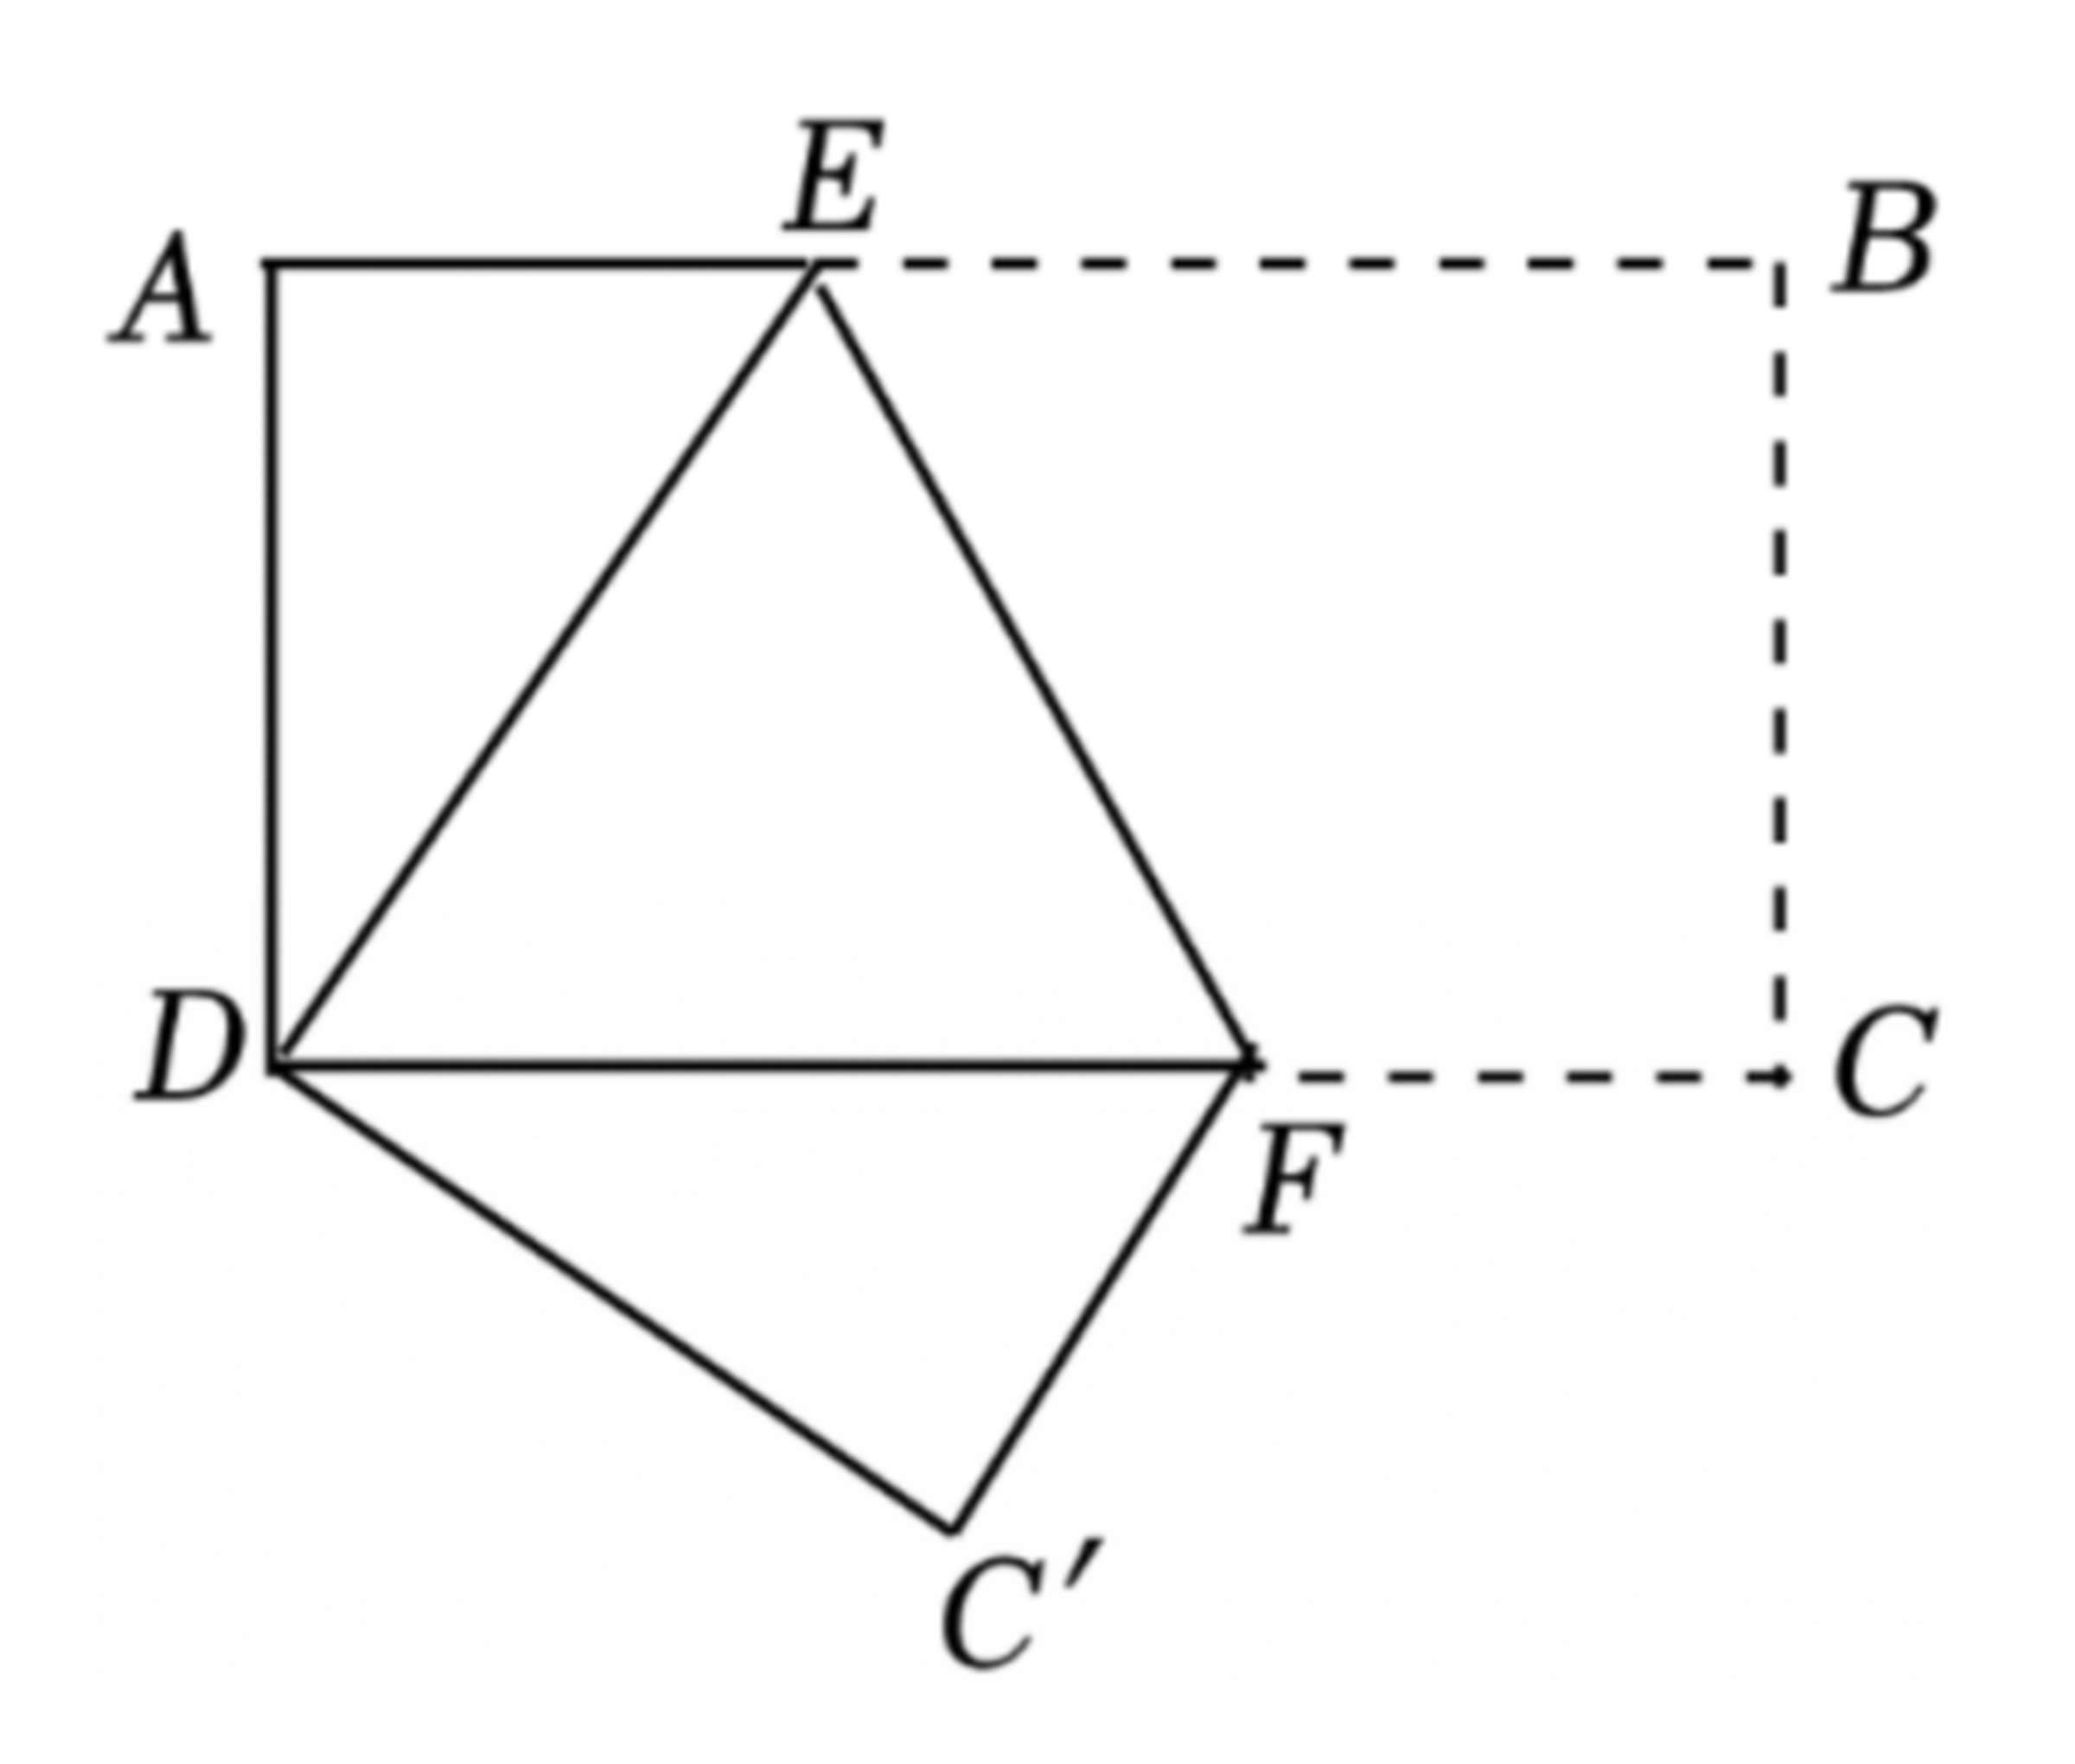
\includegraphics[width=0.40\textwidth]{figures/gao149_q11.png}
\end{center}

\ifanswer
\solbegin
\step{因为矩形 $ABCD(AB>AD)$ 的周长为 12，}
\step{在 $AB$ 和 $CD$ 边上分别取点 $E$ 和 $F$，将四边形 $BCFE$ 沿 $EF$ 折叠，}
\step{使点 $B$ 与点 $D$ 重合，此时点 $C$ 的对应点为 $C'$，}
\step{所以设 $AD=a$，$AB=b$，则 $2(a+b)=12$，}
\step{所以 $a+b=6$，且 $AB>AD$，所以 $b>a>0$，}
\step{设 $DF=x$，则 $C'F=b-x$，在 $Rt\triangle DC'F$ 中，$DC'=BC=a$，}% 几何三角形符号原卷印扁等边细线三角 $\triangle$，照录（放大 02 页确认）；$Rt$ 照录
\step{所以 $a^2+(b-x)^2=x^2$，解得 $x=\dfrac{a^2+b^2}{2b}$，}
\step{因此 $\triangle C'DF$ 的面积 $S=\dfrac{1}{2}\cdot DC'\cdot C'F=\dfrac{1}{2}\cdot a\cdot(b-x)$，}
\step{又 $b-x=b-\dfrac{(6-b)^2+b^2}{2b}=\dfrac{6(b-3)}{b}$，}
\step{所以 $S=\dfrac{1}{2}\cdot a\cdot\dfrac{6(b-3)}{b}=\dfrac{1}{2}\cdot(6-b)\cdot\dfrac{6(b-3)}{b}=\dfrac{3(6-b)(b-3)}{b}$}
\step{$=3\cdot\left(-b-\dfrac{18}{b}+9\right)$，又 $b+\dfrac{18}{b}\geqslant2\sqrt{b\cdot\dfrac{18}{b}}=6\sqrt{2}$，}
\step{当且仅当 $b=\dfrac{18}{b}$ 即 $b=3\sqrt{2}$ 时取等号，此时满足 $b>a$，}
\step{所以 $S\leqslant3\cdot(-6\sqrt{2}+9)=27-18\sqrt{2}$，故 $\triangle C'DF$ 面积的最大值为 $27-18\sqrt{2}$.}
\solend
\fi

% === Q12 === 解析内 3 幅三次函数曲线坐标图（仅答案版出）；解析 15 行（8 行 03 页＋7 行 04 页）
\item 已知 $m>0$，若存在 $t\in\R$，使得对任意 $x\in[0,m]$，不等式 $[(x-1)^2-t](x-t)\leqslant0$ 恒成立，则 $m$ 的最大值是\blankline[4.4em].

\ifanswer
\solbegin
\step{当 $t\leqslant0$ 时，$(x-1)^2-t\geqslant0$ 恒成立，}
\step{不等式 $[(x-1)^2-t](x-t)\leqslant0$ 的解集为 $x\leqslant t$，与 $x\in[0,m]$ 矛盾；}
\step{当 $t>0$ 时，不等式 $[(x-1)^2-t](x-t)\leqslant0\Leftrightarrow(x-1-\sqrt t)(x-1+\sqrt t)(x-t)\leqslant0$，}
\step{若 $t<1-\sqrt t$，即 $t\in\left(0,\dfrac{3-\sqrt5}{2}\right)$，}
\begin{center}
% 情形一 $t<1-\sqrt t$ 曲线图取 03 页右侧，去粉色水印、去色、4× LANCZOS 放大；仅答案版出
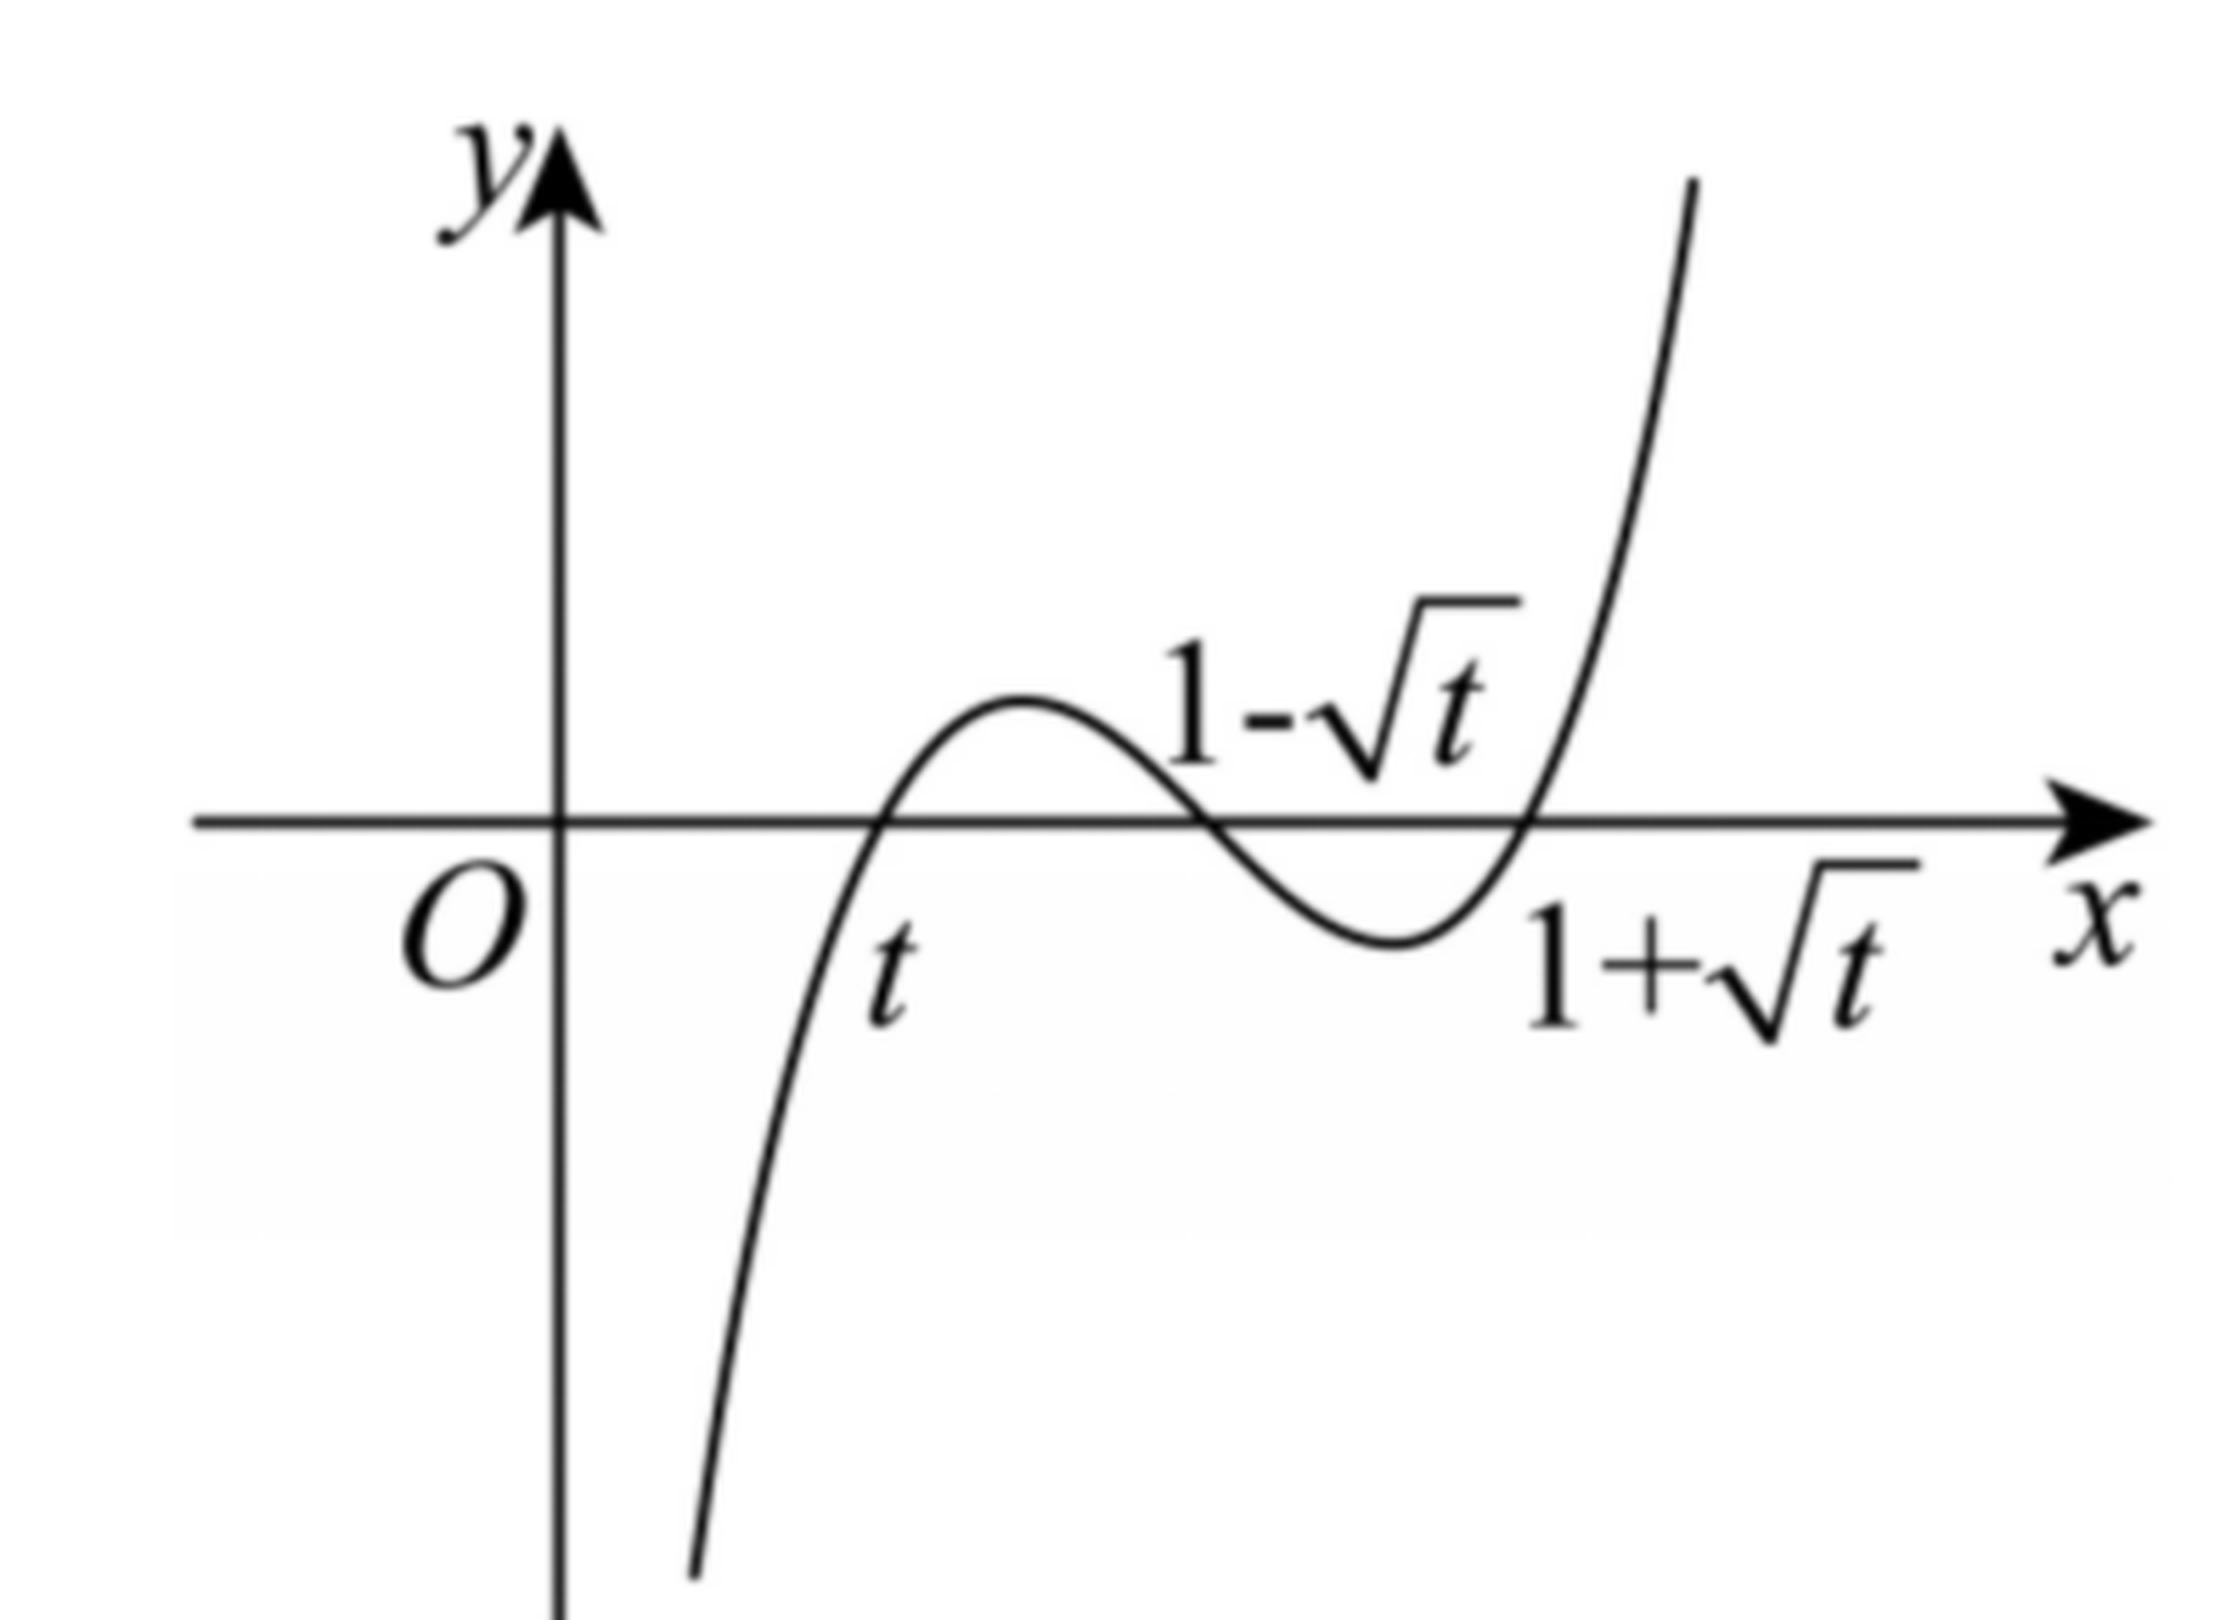
\includegraphics[width=0.40\textwidth]{figures/gao149_q12_a.png}
\end{center}
\step{则原不等式的解集为 $(-\infty,t]\cup[1-\sqrt t,1+\sqrt t]$，}
\step{当 $0<m\leqslant t$ 时，原不等式恒成立，因此}
\step{$m\in\left(0,\dfrac{3-\sqrt5}{2}\right)$；}
\step{若 $t=1-\sqrt t$，即 $t=\dfrac{3-\sqrt5}{2}$，则原不等式的解集为 $(-\infty,1+\sqrt t]$，}
\begin{center}
% 情形二 $t=1-\sqrt t$ 曲线图取 03 页右侧，去粉色水印、去色、4× LANCZOS 放大；仅答案版出
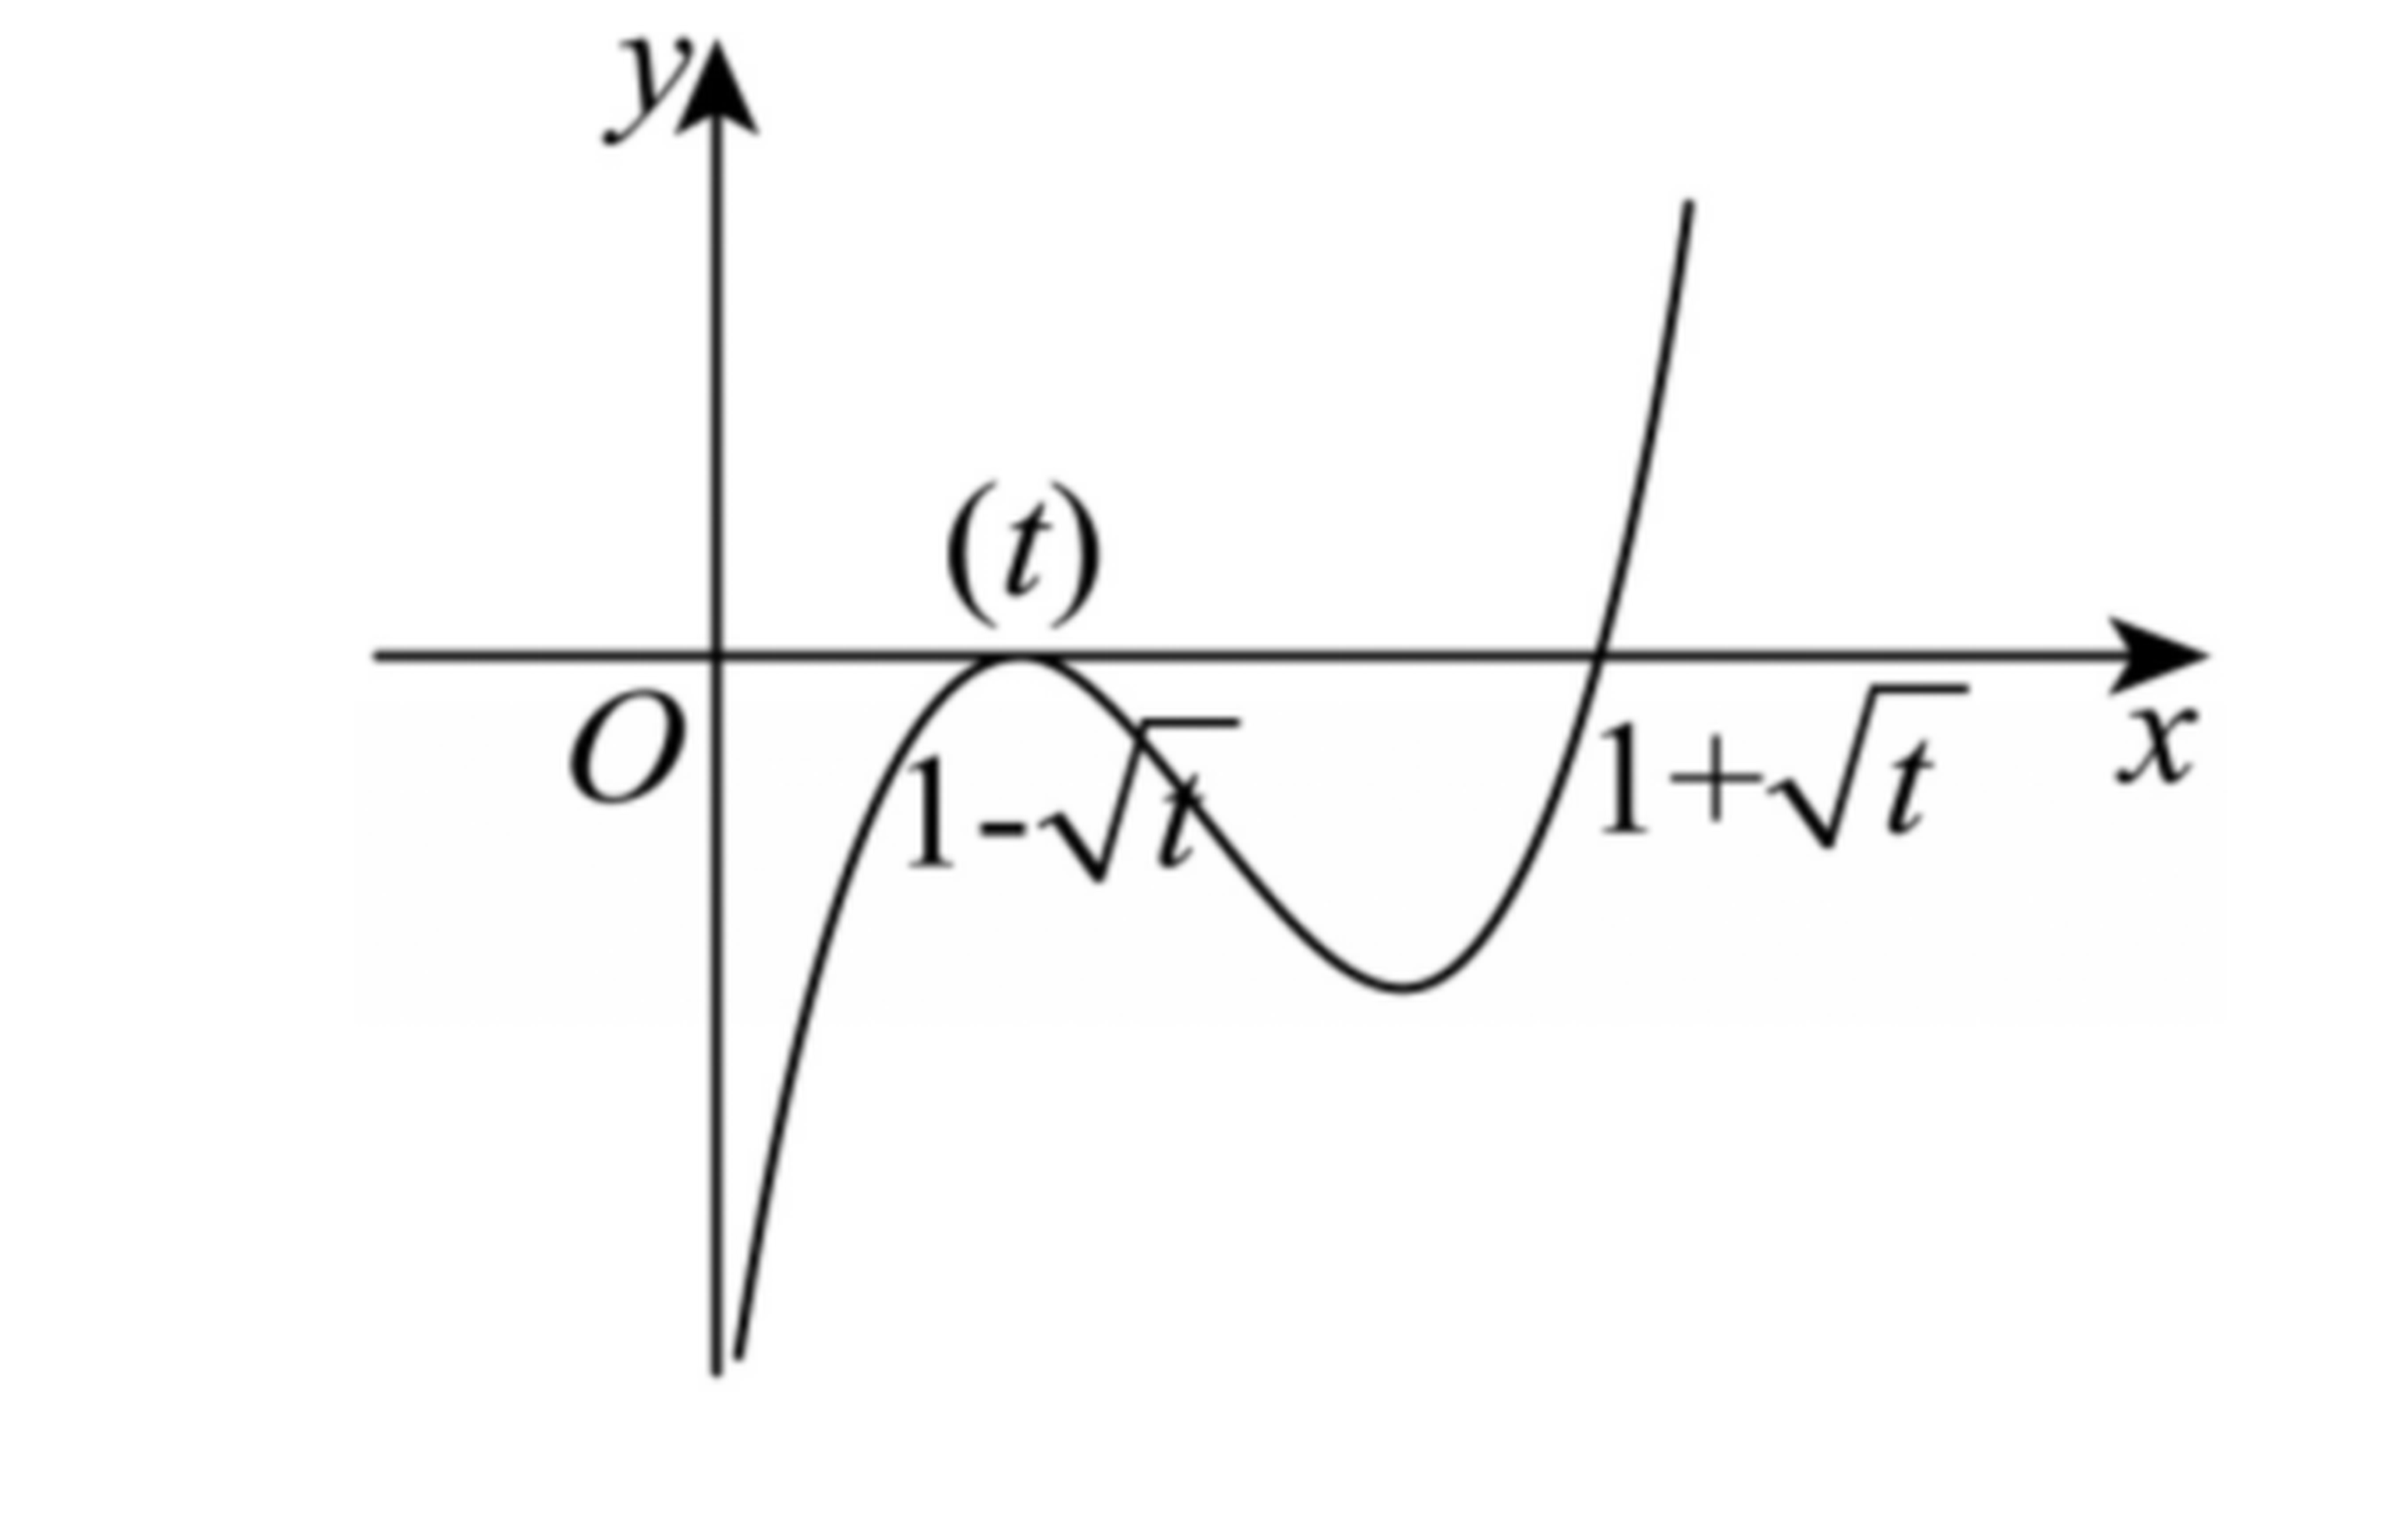
\includegraphics[width=0.40\textwidth]{figures/gao149_q12_b.png}
\end{center}
\step{当 $0<m\leqslant1+\sqrt t$ 时，原不等式恒成立，因此 $m\in\left(0,\dfrac{\sqrt5+1}{2}\right]$；}
\step{若 $1+\sqrt t>t>1-\sqrt t$，即 $t\in\left(\dfrac{3-\sqrt5}{2},\dfrac{3+\sqrt5}{2}\right)$，}
\begin{center}
% 情形三 $1+\sqrt t>t>1-\sqrt t$ 曲线图取 04 页右侧，去粉色水印、去色、4× LANCZOS 放大；仅答案版出
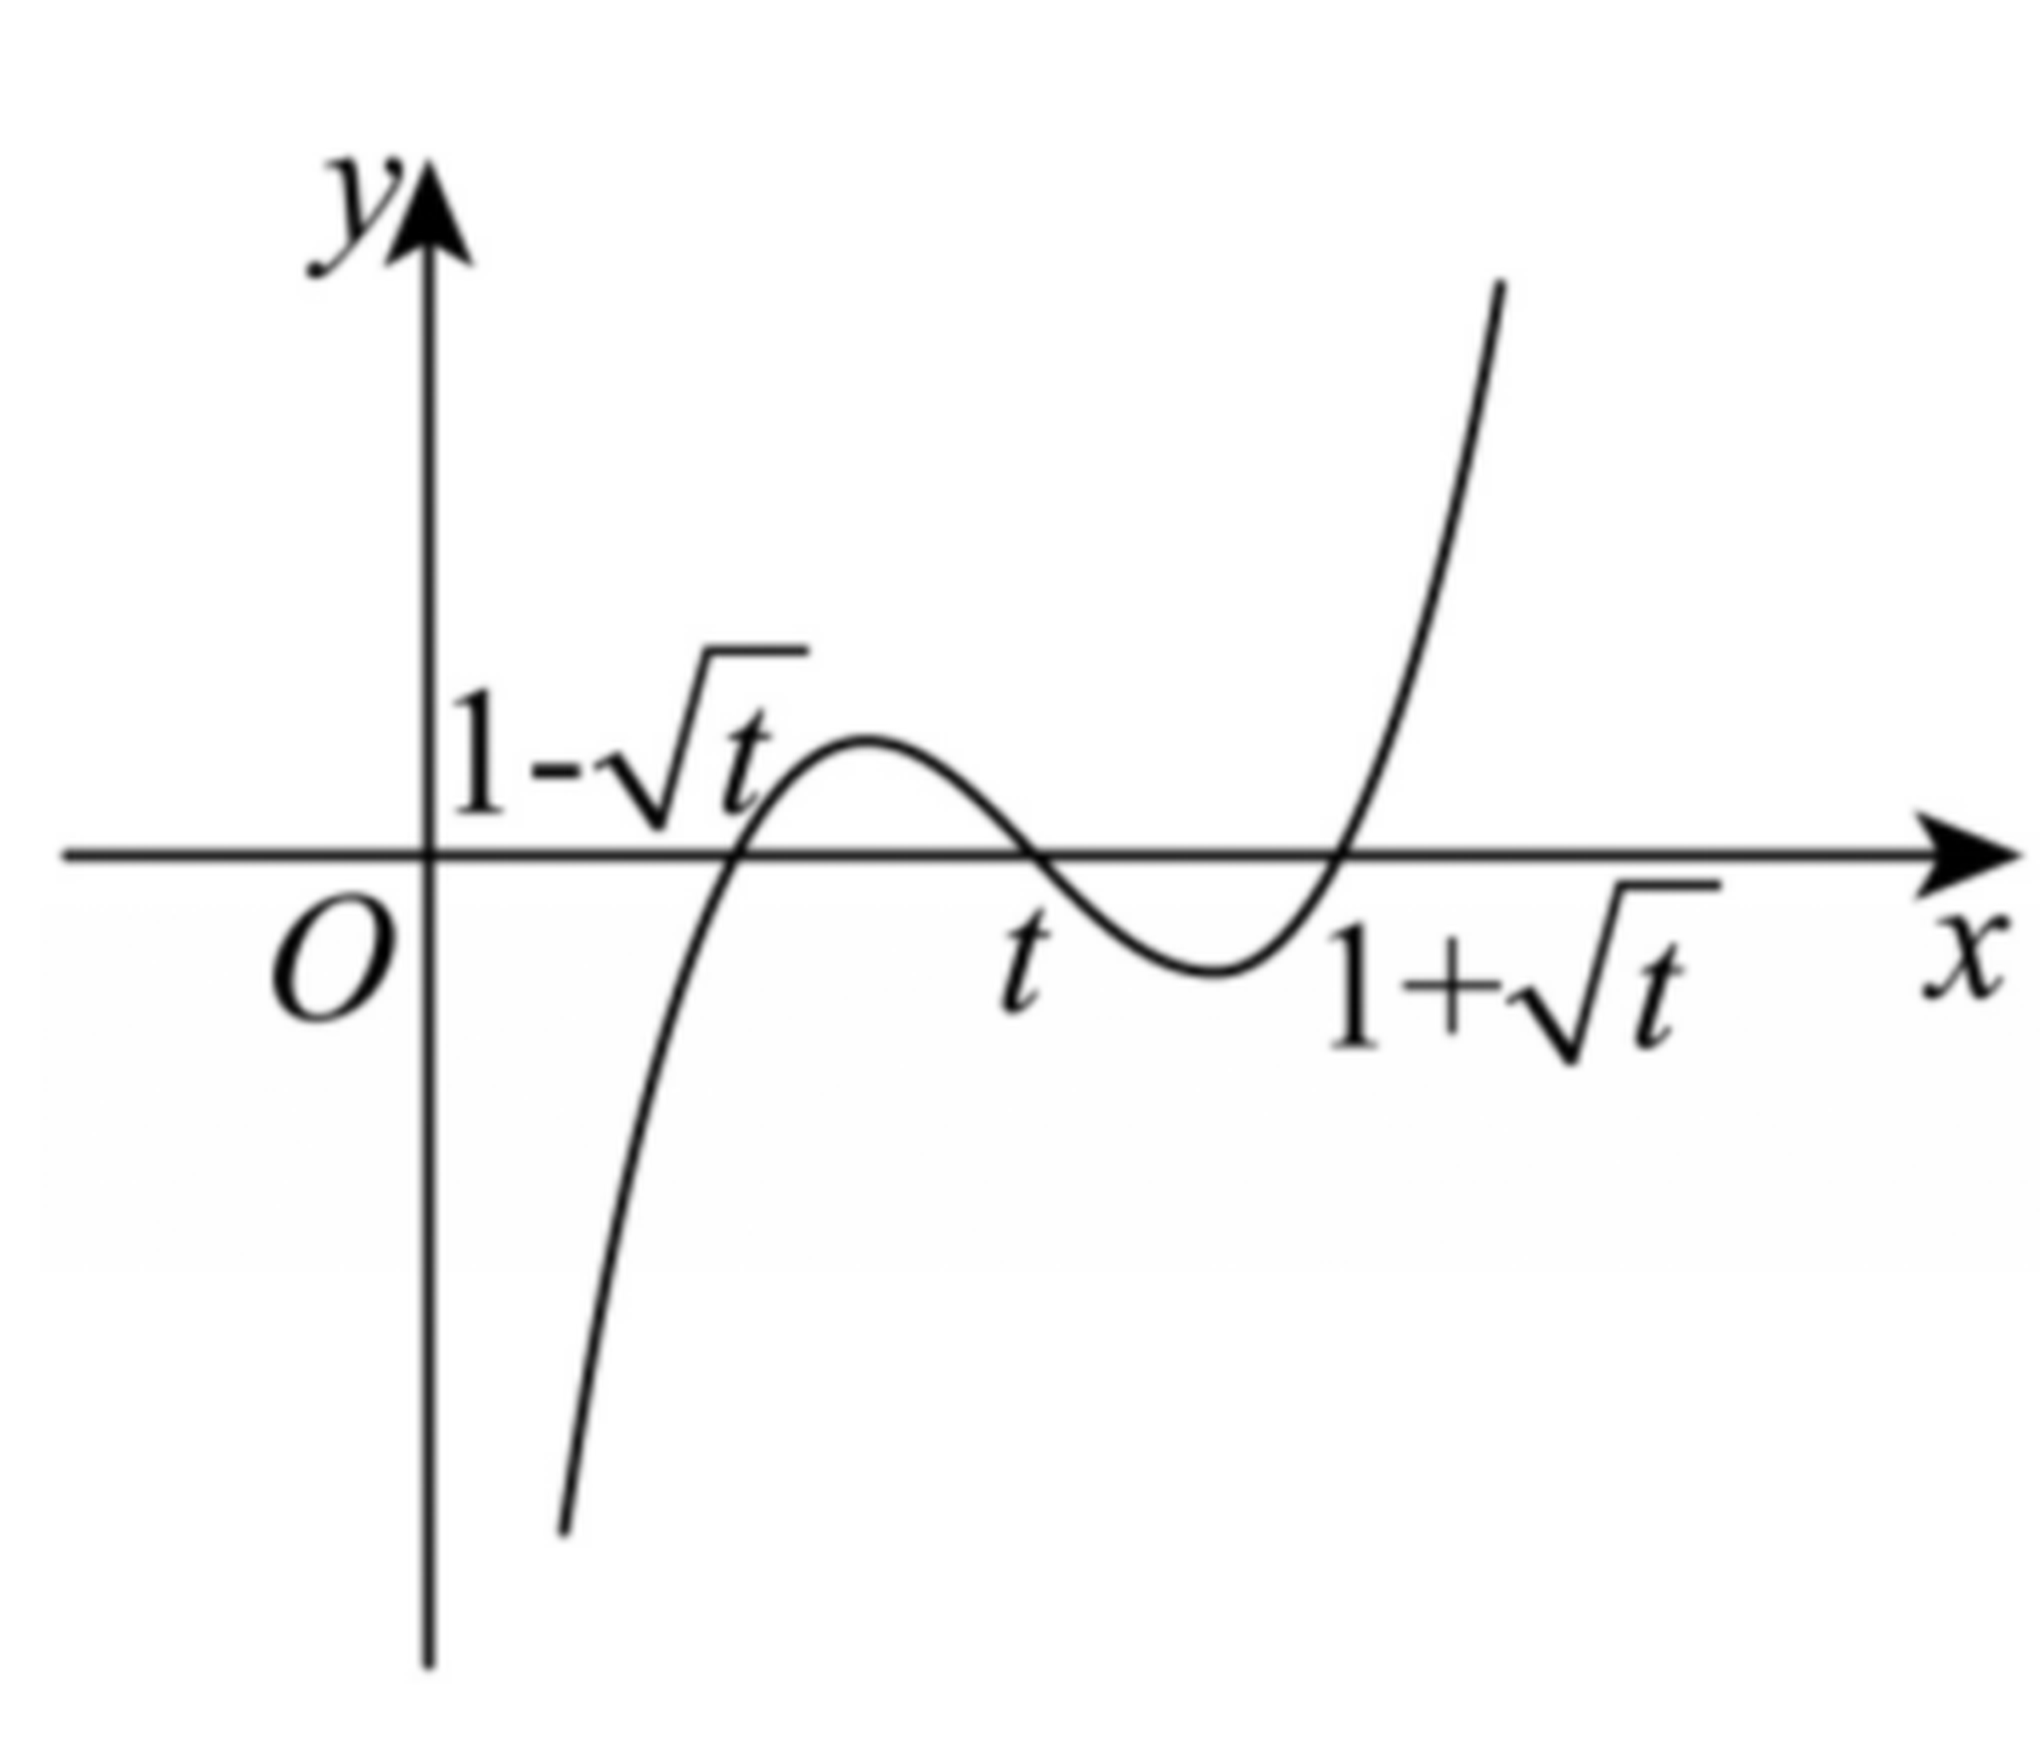
\includegraphics[width=0.40\textwidth]{figures/gao149_q12_c.png}
\end{center}
\step{则原不等式的解集为 $(-\infty,1-\sqrt t]\cup[t,1+\sqrt t]$，}
\step{当 $\begin{cases}1-\sqrt t>0\\1-\sqrt t\geqslant m\end{cases}$ 时，原不等式恒成立，此时 $t\in\left(\dfrac{3-\sqrt5}{2},1\right)$，$m\in\left(0,\dfrac{3-\sqrt5}{2}\right)$；}
\step{若 $t\geqslant1+\sqrt t$，即 $t\geqslant\dfrac{3+\sqrt5}{2}$，则取 $x=0$，$(t-1)t>0$，}
\step{原不等式不恒成立，不符合题意，}
\step{因此实数 $m$ 的取值范围是 $\left(0,\dfrac{\sqrt5+1}{2}\right]$，$m$ 的最大值是 $\dfrac{\sqrt5+1}{2}$.}
\solend
\fi

\end{enumerate}

\bigsec{二、选择题}

\begin{enumerate}
\setcounter{enumi}{12}

% === Q13 ===：答案"C"直接印在题干括号内、无【答案】/【解析】段，按 高一84 Q13／高一148 Q13 成例括号留空、另提 \ans{$C$}；四选项两行两列照原卷分行
\item 设 $ab>0$，则 $a>b$ 是 $\dfrac{1}{a}<\dfrac{1}{b}$ 的\mbox{（\quad）}

\keepwithprev
A. 充分不必要条件\qquad\qquad B. 必要不充分条件

C. 充要条件\qquad\qquad D. 既不充分又不必要条件

\ifanswer
\ans{$C$}
\fi

% === Q14 ===：$A\subset B$ 单线照录；四选项补集照原卷上划线 \overline{A}／\overline{B}；解析 1 行（由韦恩图得 B 对）
\item 已知集合 $A$、$B$ 非空，且 $A\subset B$，则下列式子中一定是空集的为\mbox{（\quad）}

\keepwithprev
A. $\overline{A}\cap B$\qquad B. $A\cap\overline{B}$\qquad C. $\overline{A}\cap\overline{B}$\qquad D. $\overline{A}\cup\overline{B}$

\ifanswer
\solbegin
\step{由韦恩图得 $B$ 对. 故选 $B$.}
\solend
\fi

% === Q15 ===："天文数字"弯引号照录；解析 2 行（首行在 04 页末、末行续 05 页顶）
\item 历史上数学计算方面的三大发明是阿拉伯数字、十进制和对数，其中对数的发明，大大缩短了计算时间，为人类研究科学和了解自然起了重大作用，对数运算对估算“天文数字”具有独特的优势. $2.5^{1000}$ 的估算值约为\mbox{（\quad）}

\keepwithprev
A. $10^{365}$\qquad B. $10^{379}$\qquad C. $10^{389}$\qquad D. $10^{398}$

\ifanswer
\solbegin
\step{$\lg 2.5^{1000}=1000\lg 2.5=1000(1-2\lg 2)\approx1000\times(1-0.602)=398$，}
\step{所以 $2.5^{1000}\approx10^{398}$. 故选 $D$.}
\solend
\fi

% === Q16 ===："完美集"新定义、圈数字①②文本模式；题干"若对任意 $x$，$y\in A$"用全角逗号、解析用顿号"$x$、$y\in A$"，两处照录不统一；解析 9 行
\item 设全集 $U=\R$，集合 $A$ 是一个非空数集，若对任意 $x$，$y\in A$，都有 $x+y\in A$、$xy\in A$，则称集合 $A$ 为一个“完美集”，给出以下命题：

①若 $A_1$、$A_2$ 都是“完美集”，且 $A_1\cap A_2\ne\varnothing$，则 $A_1\cap A_2$ 也是“完美集”；

②若 $A_1$、$A_2$ 都是“完美集”，则 $A_1\cup A_2$ 也是“完美集”.

下列说法正确的是\mbox{（\quad）}

\keepwithprev
A. ①②都是真命题\qquad\qquad B. ①是真命题，②是假命题

C. ①是假命题，②是真命题\qquad\qquad D. ①②都是假命题

\ifanswer
\solbegin
\step{由题意，全集 $U=\R$，集合 $A$ 是一个非空数集，}
\step{若对任意 $x$、$y\in A$，都有 $x+y\in A$、$xy\in A$，则称集合 $A$ 为一个“完美集”，}
\step{对于①，取 $x$、$y\in A_1\cap A_2$，则 $x\in A_1$，$x\in A_2$，$y\in A_1$，$y\in A_2$，}
\step{又 $A_1$、$A_2$ 是“完美集”，所以 $x+y\in A_1$，$xy\in A_1$，$x+y\in A_2$，$xy\in A_2$，}
\step{所以 $x+y\in A_1\cap A_2$，$xy\in A_1\cap A_2$，所以 $A_1\cap A_2$ 是“完美集”，故①正确；}
\step{对于②，取“完美集” $A_1=\{x\mid x=2k,k\in\Z\}$，$A_2=\{x\mid x=3k,k\in\Z\}$，}
\step{则 $2\in A_1$，$3\in A_2$，但 $2+3\notin A_1\cup A_2$，}
\step{即此时 $A_1\cup A_2$ 不是“完美集”，故②错误.}
\step{故选 $B$.}
\solend
\fi
\end{enumerate}

\bigsec{三、解答题}

\begin{enumerate}
\setcounter{enumi}{16}

% === Q17 ===："图像"（有亻）照录（Q17 题干与解析共 2 处）；绝对值 \lvert…\rvert；解析 7 行
\item 已知 $m\in\R$，$f(x)=(m^2-m-5)x^m$. 若 $y=f(x)$ 是幂函数，且其图像不经过原点.

(1) 求实数 $m$ 的值；

(2) 若 $f(a)=f(b)$ 且 $a\ne b$，求 $\lvert a+2\rvert+\lvert b-1\rvert$ 的最小值，并指出取到最小值时 $a$ 的取值范围.

\ifanswer
\solbegin
\step{(1) $f(x)=(m^2-m-5)x^m$ 是幂函数，得 $m^2-m-5=1$，即 $m^2-m-6=0$，}
\step{解得 $m=-2$ 或 $m=3$，又函数图像不经过原点，所以 $m=-2$($3$ 舍)；}
\step{(2) 由 (1) 得 $f(x)=x^{-2}=\dfrac{1}{x^2}$ 为偶函数，}
\step{$x<0$ 时，函数 $f(x)$ 严格增，$x>0$ 时，函数 $f(x)$ 严格减，}
\step{又 $f(a)=f(b)$ 且 $a\ne b$，所以 $a=-b$，且 $a\ne0$，$b\ne0$，}
\step{则 $\lvert a+2\rvert+\lvert b-1\rvert=\lvert a+2\rvert+\lvert-a-1\rvert=\lvert a+2\rvert+\lvert a+1\rvert$，}
\step{则 $\lvert a+2\rvert+\lvert b-1\rvert$ 的最小值为 $1$，取到最小值时 $a$ 的取值范围是 $[-2,-1]$.}
\solend
\fi

% === Q18 ===：判别式两形混用——(1) cases 块印高 \Delta、(2) 独立行印扁 \triangle，逐处照录不统一；解析 8 行
\item 已知命题 $p$：方程 $x^2+4x+m-1=0$ 有两个不等的负根；命题 $q$：方程 $4x^2+4x+m-2=0$ 无实根.

(1) 若 $p$ 为真命题，求 $m$ 的取值范围；

(2) 若 $p$、$q$ 两命题一真一假，求 $m$ 的取值范围.

\ifanswer
\solbegin
\step{(1) 若 $p$ 为真命题，即方程 $x^2+4x+m-1=0$ 有两个不等的负根；}
\step{必有 $\begin{cases}\Delta=16-4(m-1)>0\\m-1>0\end{cases}$，解得 $1<m<5$，即 $m$ 的取值范围为 $(1,5)$；}
\step{(2) 命题 $q$：方程 $4x^2+4x+m-2=0$ 无实根，}
\step{则有 $\triangle=16-16(m-2)<0$，解得 $m>3$，}
\step{若 $p$ 和 $q$ 有且只有一个为真命题，}
\step{若 $p$ 真 $q$ 假，必有 $\begin{cases}1<m<5\\m\leqslant3\end{cases}$，则有 $1<m\leqslant3$，}
\step{若 $p$ 假 $q$ 真，必有 $\begin{cases}m\leqslant1\text{ 或 }m\geqslant5\\m>3\end{cases}$，则有 $m\geqslant5$，}
\step{综上，$1<m\leqslant3$ 或 $m\geqslant5$.}
\solend
\fi

% === Q19 ===：$A\subseteq B$ 带下划线照录；解析 7 行（(2) 两组 cases 并排）
\item 已知 $m\in\R$，集合 $A=\left\{x\mid y=\sqrt{3-x}-\dfrac{1}{\sqrt{x-1}}\right\}$，集合 $B=\{x\mid 2m\leqslant x\leqslant1-m\}$.

(1) 若 $A\cup B=B$，求实数 $m$ 的取值范围；

(2) 若 $A\cap B=\varnothing$，求实数 $m$ 的取值范围.

\ifanswer
\solbegin
\step{(1) 函数 $y=\sqrt{3-x}-\dfrac{1}{\sqrt{x-1}}$，则 $\begin{cases}3-x\geqslant0\\x-1>0\end{cases}$，解得 $1<x\leqslant3$，}
\step{所以 $A=\{x\mid1<x\leqslant3\}$，}
\step{因为 $A\cup B=B$，所以 $A\subseteq B$，则 $\begin{cases}2m\leqslant1\\1-m\geqslant3\end{cases}$，解得 $m\leqslant-2$，}
\step{综上，实数 $m$ 的取值范围为 $(-\infty,-2]$；}
\step{(2) 当 $B=\varnothing$ 时，则 $2m>1-m$，解得 $m>\dfrac{1}{3}$，}
\step{当 $B\ne\varnothing$ 时，则 $\begin{cases}2m\leqslant1-m\\2m>3\end{cases}$ 或 $\begin{cases}2m\leqslant1-m\\1-m\leqslant1\end{cases}$，解得 $m\in\varnothing$ 或 $0\leqslant m\leqslant\dfrac{1}{3}$，}
\step{综上，实数 $m$ 的取值范围为 $[0,+\infty)$.}
\solend
\fi

% === Q20 ===：n 阶基本不等式推广；(3) 解析含 \overbrace{…}^{k} 上括号；(2) 解析"x=x=x=3(1-x)"三连等系原卷笔误、照录加注（见 ⑤）；解析 14 行
\item 教材中的基本不等式可以推广到 $n$ 阶：$n$ 个正数的算术平均数不小于它们的几何平均数，即对于任意的正数 $a_1$、$a_2$、$\cdots$、$a_n$，有 $\dfrac{a_1+a_2+\cdots+a_n}{n}\geqslant\sqrt[n]{a_1\cdot a_2\cdots a_n}$（$n\in\N$ 且 $n\geqslant2$），且等号当且仅当 $a_1=a_2=\cdots=a_n$ 时成立. 利用此结论解决下列问题：

(1) 若 $x$、$y$、$z>0$，求 $\dfrac{y}{x}+\dfrac{2z}{y}+\dfrac{4x}{z}$ 的最小值；

(2) 已知 $0<x<1$，求 $x^3(1-x)$ 的最大值，并求取得最大值时的 $x$ 的值；

(3) 对任意的正整数 $k$，判断 $\left(1+\dfrac{1}{k}\right)^k$ 与 $\left(1+\dfrac{1}{k+1}\right)^{k+1}$ 的大小关系，并证明.

\ifanswer
\solbegin
\step{(1) 因为 $x$、$y$、$z>0$，有 $\dfrac{y}{x}>0$，$\dfrac{2z}{y}>0$，$\dfrac{4x}{z}>0$}
\step{所以 $\dfrac{y}{x}+\dfrac{2z}{y}+\dfrac{4x}{z}\geqslant3\sqrt[3]{\dfrac{y}{x}\cdot\dfrac{2z}{y}\cdot\dfrac{4x}{z}}=3\sqrt[3]{8}=6$，}
\step{当且仅当 $\dfrac{y}{x}=\dfrac{2z}{y}=\dfrac{4x}{z}$ 时取等号，故 $\dfrac{y}{x}+\dfrac{2z}{y}+\dfrac{4x}{z}$ 的最小值为 $6$.}
\step{(2) 因为 $0<x<1$，所以 $1-x>0$，}
\step{$x^3(1-x)=\dfrac{1}{3}[x\cdot x\cdot x\cdot3(1-x)]\leqslant\dfrac{1}{3}\left[\dfrac{x+x+x+3(1-x)}{4}\right]^4=\dfrac{1}{3}\times\left(\dfrac{3}{4}\right)^4$}
\step{$=\dfrac{27}{256}$，当且仅当 $x=x=x=3(1-x)$，即 $x=3(1-x)$，$x=\dfrac{3}{4}$ 取等号，}% 原卷"x=x=x=3(1-x)"三连等，疑为四因子相等之误排，放大 08 页确认，照录未改（见 ⑤）
\step{所以 $0<x<1$ 时，$x^3(1-x)$ 的最大值是 $\dfrac{27}{256}$，取最大值时 $x=\dfrac{3}{4}$.}
\step{(3) 对任意 $k\in\N^*$，$\left(1+\dfrac{1}{k}\right)^k<\left(1+\dfrac{1}{k+1}\right)^{k+1}$.}
\step{证明：$\left(1+\dfrac{1}{k}\right)^k=\overbrace{\left(1+\dfrac{1}{k}\right)\cdot\left(1+\dfrac{1}{k}\right)\cdots\left(1+\dfrac{1}{k}\right)}^{k}\times1$}
\step{$\leqslant\left(\dfrac{\overbrace{\left(1+\dfrac{1}{k}\right)+\left(1+\dfrac{1}{k}\right)+\cdots+\left(1+\dfrac{1}{k}\right)}^{k}+1}{k+1}\right)^{k+1}$}
\step{$=\left(\dfrac{\overbrace{(1+1+\cdots+1)}^{k}+\overbrace{\left(\dfrac{1}{k}+\dfrac{1}{k}+\cdots+\dfrac{1}{k}\right)}^{k}+1}{k+1}\right)^{k+1}=\left(\dfrac{k+1+1}{k+1}\right)^{k+1}=\left(1+\dfrac{1}{k+1}\right)^{k+1}$，}
\step{当且仅当 $1+\dfrac{1}{k}=1$ 时取等号，}
\step{但是任意 $k\in\N^*$ 时 $1+\dfrac{1}{k}>1$，所以等号不成立，}
\step{故任意 $k\in\N^*$ 时，$\left(1+\dfrac{1}{k}\right)^k<\left(1+\dfrac{1}{k+1}\right)^{k+1}$.}
\solend
\fi

% === Q21 ===："减 k 集"新定义（引号内 k／数字两侧空格照录）；解析 26 行（续 10 页），含 ⑤ 三处原卷笔误照录
\item 定义：对于给定的整数 $k$，若非空集合 $A$ 满足如下 3 个条件：

① $A$ 是正整数集的子集；② $A\ne\{1\}$；

③对任意正整数 $x,y$，若 $x+y\in A$，则 $xy-k\in A$；则称集合 $A$ 为“减 $k$ 集”.

(1) 判断集合 $A=\{1,2\}$ 是否为“减 $0$ 集”？是否为“减 $1$ 集”？（无需说明理由）

(2) 证明：不存在“减 $2$ 集”；

(3) 是否存在“减 $1$ 集”？如果存在，求出所有“减 $1$ 集”；如果不存在，说明理由.

\ifanswer
\solbegin
\step{(1) 因为 $P\subseteq\N^*$，$P\ne\{1\}$，$1+1=2\in P$，$1\times1-0\in P$，}
\step{所以集合 $P=\{1,2\}$ 是“减 $0$ 集”；}
\step{因为 $P\subseteq\N^*$，$P\ne\{1\}$，$1+1=2\in P$，$1\times1-1\notin P$，}
\step{所以集合 $P=\{1,2\}$ 是“减 $1$ 集”；}% 按条件③应为"不是"，原卷径印"是"，放大 09 页确认，照录未改（见 ⑤）
\step{(2) 假设存在集合 $A$ 是“减 $2$ 集”，若 $x+y\in A$，则 $xy-2\in A$，}
\step{①当 $x+y=xy-2$ 时，有 $(x-1)(y-1)=3$，}
\step{则 $x$、$y$ 一个为 $2$，一个为 $4$，所以集合 $A$ 有元素 $6$，}
\step{但 $3+3\in A$，$3\times3-2\notin A$，与 $A$ 是“减 $2$ 集”矛盾；}
\step{②当 $x+y\ne xy-2$ 时，则 $x+y=xy-1$ 或 $x+y=xy-m$($m>2$)，}
\step{若 $x+y=xy-1$，$m=1$ 时，$M$ 为除 $1$ 以外的最小元素，}% 原卷"m=1"上文未显式定义，疑笔误，放大 09 页确认，照录未改（见 ⑤）
\step{则 $x=M-1$，$y=1$ 时，$xy-2=M-3$ 小于 $M$，}
\step{要符合题意，必须 $M=4$，}
\step{此时取 $x-2$，$y=2$，$xy-2=2$ 不属于 $A$，故不符合题意，}% 原卷"取 x−2"疑为"取 x=2"误排，放大 09 页确认，照录未改（见 ⑤）
\step{当 $m>2$ 时，$(x-1)(y-1)=m+1$，同样得出矛盾，}
\step{综上，不存在 $A$ 是“减 $2$ 集”.}
\step{(3) 存在“减 $1$ 集” $A$，则 $A\ne\{1\}$，}
\step{①假设 $1\in A$，则 $A$ 中除了元素 $1$ 以外，必然还含有其它元素，}
\step{假设 $2\in A$，$1+1\in A$，而 $1\times1-1\notin A$，所以 $2\notin A$，}
\step{假设 $3\in A$，$1+2\in A$，而 $1\times2-1\in A$，所以 $3\in A$，}
\step{所以 $A=\{1,3\}$，}
\step{假设 $4\in A$，$1+3\in A$，而 $1\times3-1\notin A$，所以 $4\notin A$，}
\step{假设 $5\in A$，$1+4\in A$，$1\times4-1\in A$，$2+3=5$，$2\times3-1\in A$，所以 $5\in A$，}
\step{所以 $A=\{1,3,5\}$，}
\step{以此类推，得 $A=\{1,3,5,\cdots,2n-1,\cdots\}$，($n\in\N^*$)，}
\step{所以所有的“减 $1$ 集”有 $\{1,3\}$，$\{1,3,5\}$，$\{1,3,5,7\}$，$\cdots$，$\{1,3,5,\cdots,2n-1,\cdots\}$，}
\step{$(n\in\N^*)$.}
\solend
\fi
\end{enumerate}

\end{document}
"
% 紧凑版：xelatex "\def\iscompact{1}% 高一149_青浦高级中学上外云间_期中.tex
%   —— 高一上数学"2026-2027 年青浦高级中学上外云间高一上期中"（试卷版/答案版/紧凑版）
% 试卷版：xelatex 高一149_青浦高级中学上外云间_期中.tex
% 答案版：xelatex "\def\isanswer{1}\input{高一149_青浦高级中学上外云间_期中.tex}"
% 紧凑版：xelatex "\def\iscompact{1}\input{高一149_青浦高级中学上外云间_期中.tex}"
%
% ① 原始材料：微信公众号"魔都数学加油站"文章，连载"27学年高一149"，原文标题
% "27学年高一149——2026-2027年上海市青浦高级中学上外云间高一上期中"；
% 原文链接：https://mp.weixin.qq.com/s/T7_nyoR1k0o_5og7FkDsyw 。
% 正文为 10 张 PNG 页（01/02/03/04/10 为 2560×3620，05/06/07/08/09 为 4762×6735，
% 同一篇各页分辨率混排，逐页按各自分辨率裁图核对，别按预览比例换算裁框）。
% 体例：混合体例讲评版——19 题中 Q6 只印【答案】、无【解析】；Q13 的答案"C"
%   直接印在题干括号内、无【答案】/【解析】段；其余 17 题印【解析】（逐题核实，见 ② ②）。
% 题目、答案、解析均据原图转录；卷面粉红色水印"魔都数学加油站"及公众号页脚未录入。
% 全卷插图清单（逐页通读 10 页确认）：1 幅题目配图 + 3 幅【解析】内配图：
%   · Q11 矩形 ABCD 折叠几何图（02 页右侧：A/B/C/D/E/F/C' 与虚线 EB、BC、FC），
%     题干"如图"处，题目配图、三版都出，裁 figures/gao149_q11.png；
%   · Q12【解析】内 3 幅三次函数曲线坐标图（03 页右侧两幅 + 04 页右侧一幅：
%     x/y 轴、O、t、1-\sqrt t、1+\sqrt t 等标注，分别对应 t<1-\sqrt t、
%     t=1-\sqrt t、1+\sqrt t>t>1-\sqrt t 三种情形），解析配图、仅答案版出，
%     分别裁 figures/gao149_q12_a.png／_b.png／_c.png，放 \ifanswer 内 \step 之间
%     （高一73 第 16 题成例）；
%   其余各页逐页确认无其它题目配图、无表格；Q14 解析"由韦恩图得 B 对"仅文字推导、
%   原卷并未印韦恩图；Q9／Q18／Q19 的 cases 块与 Q20(3) 的 \overbrace 为数学块（非图）；
%   10 页下半仅水印、无正文。4 图均取自原卷截图，去粉色水印、去色、4× LANCZOS 放大。
%
% 卷首标题：原卷印作"2026-2027 年青浦高级中学上外云间高一上期中"，年份区间按全稿
% 惯例排 en dash；原卷卷面未印副标题，本稿按同期中卷（高一140／141／143／144／145／
% 146／147／148）知识模块口径补出"集合与常用逻辑用语、不等式、函数"。
%
% 题号体例（逐页核实定稿）：本卷共 19 题——一、填空题 3—12（10 题）、
% 二、选择题 13—16（4 题）、三、解答题 17—21（5 题）。
% 三节分别 \setcounter{enumi}{2}／{12}／{16}。原卷从第 3 题起、无第 1、2 题，
% 本稿保留原题号；全卷无附加题节（Q21 解析末行"（n\in N^*）."为全卷收尾）。
%
% ② 与原卷的排版差异：
%   ① 原文从第 3 题起，本稿保留原题号；共 19 题三节；
%   ② 混合体例逐题核实：Q6（反证法"假设的内容"）只印【答案】、无【解析】，
%      按 高一140 第 5 题／高一145 Q3 成例提 \ans{}、不补造解析；Q13 答案"C"直接
%      印在题干括号内、全卷无该题【答案】/【解析】段，按 高一84 Q13／高一148 Q13
%      成例括号 \mbox{（\quad）} 留空、另提 \ans{$C$}；其余 17 题印【解析】、
%      用 \solbegin…\solend，选择题答案在解析末句"故选 X"（Q14 选 B、Q15 选 D、
%      Q16 选 B，逐个放大 04/05 页核实）、题干括号留空、不另提 \ans{}；
%      答案版【答案】/【解析】标记数 = 19（2 个 \ans ＋ 17 个 \solbegin）
%      = 全卷题数；
%   ③ 原卷卷面未印副标题，本稿按知识模块口径补出；
%   ④ 原卷填空横线按全稿惯例排 \blankline[4.4em]；选择题括号排 \mbox{（\quad）}、
%      选项段前按惯例加 \keepwithprev；Q13／Q16 四选项为两行两列、Q14／Q15
%      选项为一行，照原卷分行；解答题不留作答区、不加 \anspace（原卷为讲评版）；
%   ⑤ 数集：Q6"a,b\in N"、Q8"x\in R"、Q9"a\in R"／"解集为 R"、Q12"t\in R"、
%      Q16"U=R"、Q17"m\in R"、Q19"m\in R"、Q20"n\in N" 原卷印斜体 R/N，
%      按全稿惯例统一改 \R／\N；Q20(3)、Q21 的 $N^*$ 排 \N^*；Q16 解析
%      "$k\in Z$" 排 \Z。绝对值排 \lvert…\rvert（Q17），集合描述竖线排 \mid
%      （Q19、Q16 解析）；不等号按全稿惯例排 \leqslant／\geqslant；
%      补集照原卷上划线排 \overline{A}／\overline{B}（Q14 四选项）；空集
%      \varnothing（Q16、Q19、Q21）；
%   ⑥ 子集符号逐处照录不统一：Q4 题干"{1,2}⊆A⊂{1,2,3,4,5,6}" 前者印带下划线
%      ⊆、照录 \subseteq，后者印单线 ⊂、照录 \subset；Q10"A⊆{-1,1/2,2,3}"、
%      Q19 解析"A⊆B"、Q21 解析"P⊆N*" 均印带下划线 ⊆、照录 \subseteq；
%      Q14"A⊂B" 印单线 ⊂、照录 \subset（逐处放大 01/02/04/07/09 页确认，见 ④）；
%   ⑦ 子题标号 (1)(2)(3) 半角括号照录；圈数字 ①②③ 在文本模式（Q16 两命题、
%      Q21 三个条件与解析的①②）按 common.sty 划入 CJK 字符类渲染；cases 块整体
%      算一个印刷行；\left…\right 不得拆到不同 $…$ 组；数学式内 CJK 用 \text{}
%      （Q18 解析 cases 块"\text{或}"）；Q11 解析"Rt\triangle DC'F" 的 Rt 照录；
%   ⑧ 题干／解析中的中文弯引号按原卷照录：Q6" 已知 a,b\in N，若 ab 能被 5 整除，
%      那么 a、b 中至少有一个能被 5 整除 "（开引号后紧跟"已知"、闭引号后空格接"时"）、
%      Q15"天文数字"、Q16"完美集"、Q21"减 k 集""减 0 集""减 1 集""减 2 集"
%      （引号内 k／数字两侧有空格），注释内一律 ASCII 引号；
%   ⑨ 半角逗号在数学组之间是全稿惯例、非笔误（Q8"$a>0,a\ne1,x\in\R$"、
%      Q21 题干"$x,y$" 等），逐处照录别改；Q16 题干"若对任意 $x$，$y\in A$"
%      用全角逗号而解析用顿号"$x$、$y\in A$"，两处不同均照录；行末西文句点
%      照录为 ASCII `.`；行中全角逗号／顿号照录；
%   ⑩ "图像／图象"逐处放大核：Q10 题干与解析共 6 处均印"图象"（象，无亻）；
%      Q17 题干"其图像不经过原点"与解析"又函数图像不经过原点" 2 处印"图像"
%      （像，有亻），逐处照录未统一改动（放大 02/05/06 页确认）；
%   ⑪ 判别式 Δ/△ 混用是照录项：Q9 解析 cases 块"Δ=4(a−2)²+16(a−2)<0"、
%      Q18(1) cases 块"Δ=16−4(m−1)>0" 两处印等腰偏高粗三角 \Delta；
%      Q18(2) 独立行"△=16−16(m−2)<0" 印扁等边细线三角 \triangle，
%      逐处放大判断、照录不统一（参照 高一142／144／145／146／148 头注④口径）；
%      另 Q11 题干"△C'DF 面积"与解析 3 处"△"（含"Rt△DC'F"）共 4 处几何
%      三角形符号亦印扁细线三角，照录 \triangle（非判别式，字形同类，见 ④）；
%   ⑫ 一条 \step = 原卷解析的一个印刷行，cases 块整体算一个印刷行；别把原卷折行
%      并起来、别把一行拆多条。Q11 十三行（7 行在 02 页＋6 行在 03 页）、
%      Q12 十五行（8 行在 03 页＋7 行在 04 页）、Q16 九行、Q21 二十六行
%      （续 10 页）均按印刷行逐条断，不丢行；
%   ⑬ 配图：Q11 题目配图（三版都出）放 \item 内题干之后 \begin{center}，
%      大图块加 \needvspace{8cm} 守卫把整块推走（守卫放 \item 之前，见
%      高一145 Q14/Q20 成例与切页审计 B 类坑）；Q12 三幅解析配图（仅答案版出）
%      放 \ifanswer 内 \solbegin…\solend 的 \step 之间；三版切页审计均"合计异常：无"；
%   ⑭ 跨页续印按题合并：Q3/4/5 在 01 页；Q6/7/8 题干与解析在 01 页；
%      Q9 题干在 01 页末、解析 4 行在 02 页顶；Q10 题干＋解析在 02 页；
%      Q11 题干＋图＋解析前 7 行在 02 页、解析后 6 行续 03 页顶；
%      Q12 题干＋解析首行在 03 页末、解析续 7 行在 03 页下半＋7 行在 04 页顶，
%      "二、选择题"标题在 04 页下半；Q13/14 题干＋选项＋Q14 解析在 04 页下半；
%      Q15 题干＋选项＋解析首行在 04 页末、末行"所以 2.5^1000≈10^398. 故选 D."
%      续 05 页顶；Q16 题干＋选项＋解析 9 行在 05 页、"三、解答题"标题＋
%      Q17 题干首句在 05 页末；Q17(2)＋解析 7 行、Q18 题干＋解析前 6 行在 06 页；
%      Q18 解析末 2 行续 07 页顶；Q19 题干＋解析 4 行在 07 页上半、
%      解析续 3 行在 07 页下半；Q20 题干(1) 在 07 页末、题干(2)(3)＋解析(1)(2)
%      在 08 页上半、(3) 解析含 \overbrace 的证明在 08 页下半、末行
%      "故任意 k∈N* 时…"续 09 页顶；Q21 题干＋解析(1)(2)(3) 前段在 09 页、
%      解析(3) 后半 9 行续 10 页上半（10 页下半仅水印、无正文）。
%      本稿按题连排，不丢行、不并折行；
%   ⑮ 原卷解析内无红色"法一／法二"之类小标题，故本卷无 \stepm；水印
%      "魔都数学加油站"红色不录入。
%
% ③ 行数复核：一条 \step／\stepm = 原卷解析的一个印刷行，cases 块作一个印刷行计。
%   逐题数（主会话逐页核对定稿）：Q3：1；Q4：2；Q5：2；Q6：0（只印【答案】、
%   提 \ans{}）；Q7：1；Q8：1；Q9：4；Q10：5；Q11：13；Q12：15；
%   Q13：0（答案印在题干括号内、另提 \ans{}）；Q14：1；Q15：2；Q16：9；
%   Q17：7；Q18：8；Q19：7；Q20：14；Q21：26。
%   合计 118 条 \step（本卷无 \stepm：解析内无红色"法一／法二"类小标题），
%   与原卷逐题印刷行相等。全卷 17 题设 \solbegin…\solend ＋ 2 处 \ans{}，
%   答案版【答案】/【解析】标记数 = 19 = 全卷题数。
%
% ④ 判别式／子集符号结论（逐处放大原图照录、不得统一，主会话像素级复核）：
%   判别式全卷 3 处，两形混用逐处照录不统一（参照 高一142／144／145／146／148 头注④）：
%     · Q9 解析 cases 块"Δ=4(a−2)²+16(a−2)<0" 原卷印等腰偏高粗三角（高>宽、
%       粗笔画），照录 \Delta（放大 02 页 /tmp/gao149/z/t02_q9_delta2.png 确认）；
%     · Q18(1) cases 块"Δ=16−4(m−1)>0" 原卷印等腰偏高粗三角（高>宽、粗笔画），
%       照录 \Delta（放大 06 页 /tmp/gao149/z/t06_q18a.png 确认）；
%     · Q18(2) 独立行"△=16−16(m−2)<0" 原卷印扁等边细线三角（宽>高、细线），
%       照录 \triangle（放大 06 页 /tmp/gao149/z/t06_q18b.png 与 Q18(1) 并排确认）。
%   另 Q11 题干"△C'DF"与解析 3 处"△"（含"Rt△DC'F"）共 4 处几何三角形符号
%     亦印扁等边细线三角，照录 \triangle（放大 02 页
%     /tmp/gao149/z/t02_q11_tri2.png 确认），与 Q9／Q18(1) 判别式 \Delta 两形不统一。
%   子集／补集：Q4 题干"{1,2}⊆A⊂{1,2,3,4,5,6}" 前者带下划线 ⊆、照录 \subseteq，
%     后者单线 ⊂、照录 \subset（放大 01 页 /tmp/gao149/z/t01_q3q4.png 确认）；
%     Q10"A⊆{-1,1/2,2,3}"、Q19 解析"A⊆B"、Q21 解析"P⊆N*" 三处带下划线 ⊆、
%     照录 \subseteq；Q14"A⊂B" 单线 ⊂、照录 \subset（放大 04 页
%     /tmp/gao149/z/t04_q14_sub2.png 确认）；Q14 四选项补集 \overline{A}／\overline{B}
%     照原卷上划线；空集 \varnothing（Q16、Q19、Q21）；Q19／Q16 解析集合描述竖线
%     \mid；数集 \R／\N／\N^*／\Z 归一见 ② ⑤。
%
% ⑤ 存疑照录（放大原图确认，照录未改、正文对应处另有 % 注）：
%   1. Q21 解析(1) 第二组"因为 P⊆N*，P≠{1}，1+1=2∈P，1×1−1∉P，所以集合
%      P={1,2} 是"减 1 集"" —— 按条件③（x=y=1 时 xy−1=0 须∈P）应为"不是"，
%      原卷却径印"是"，放大 09 页 /tmp/gao149/z/t09_q21_sol1.png 确认，照录未改
%      （疑为原卷结论笔误）。
%   2. Q21 解析(2)"此时取 x−2，y=2，xy−2=2 不属于 A" —— 按上下文应为
%      "取 x=2"（x−2 疑为 x=2 的误排），放大 09 页
%      /tmp/gao149/z/t09_q21_sol2.png 确认，照录未改。
%   3. Q21 解析(2)"若 x+y=xy−1，m=1 时，M 为除 1 以外的最小元素" 中 $m=1$
%      上文未显式定义 m（仅"x+y=xy−m(m>2)"中出现），放大 09 页确认，照录未改。
%   4. Q20 解析(2)"当且仅当 x=x=x=3(1−x)" 三个 x 连等，疑为原卷排印（应为
%      四个因子 x,x,x,3(1−x) 相等），放大 08 页
%      /tmp/gao149/z/t08_q20_sol2.png 确认，照录未改。
%   5. Q6 只印【答案】、Q13 答案印题干括号内，两题均无【解析】，按成例提
%      \ans{}、未补造解析（见 ② ②）。
%   6. 判别式 Q9／Q18(1) 高 \Delta 与 Q18(2)／Q11 扁 \triangle 两形混用，逐处
%      照录不统一（见 ④）；"图像／图象" Q10 用"图象"、Q17 用"图像"，
%      逐处照录未统一（见 ② ⑩）。
%   全卷除此 6 类外未发现其它笔误／自相矛盾处。
%
% ⑥ 跨页续印按题合并说明：见 ② ⑭。
%
\documentclass[a4paper,11pt]{article}
\usepackage{common}

\begin{document}

\examtitlest[3]{2026--2027 年青浦高级中学上外云间高一上期中}{集合与常用逻辑用语、不等式、函数}

\bigsec{一、填空题}

\begin{enumerate}
\setcounter{enumi}{2}

% === Q3 === 根式化分数指数幂；解析 1 行
\item 根式 $\sqrt{a\sqrt a}$ 化成分数指数幂是\blankline[4.4em].

\ifanswer
\solbegin
\step{$\sqrt{a\sqrt a}=\sqrt{a\cdot a^{\frac{1}{2}}}=\sqrt{a^{1+\frac{1}{2}}}=\sqrt{a^{\frac{3}{2}}}=a^{\frac{3}{2}\times\frac{1}{2}}=a^{\frac{3}{4}}$.}
\solend
\fi

% === Q4 === 题干两种子集符号逐处照录（\subseteq 带下划线／\subset 单线）；解析 2 行
\item 满足 $\{1,2\}\subseteq A\subset\{1,2,3,4,5,6\}$ 的集合 $A$ 共有\blankline[4.4em]个.

\ifanswer
\solbegin
\step{集合 $A$ 满足 $\{1,2\}\subseteq A\subset\{1,2,3,4,5,6\}$，}% 前者带下划线 $\subseteq$、后者单线 $\subset$，逐处照录不统一（放大 01 页确认）
\step{所以集合 $A$ 的个数为集合 $\{3,4,5,6\}$ 的真子集的个数，即为 $2^4-1=15$ 个.}
\solend
\fi

% === Q5 === 解析 2 行
\item 不等式 $\dfrac{2x+1}{x-1}\leqslant0$ 的解集为\blankline[4.4em].

\ifanswer
\solbegin
\step{不等式 $\dfrac{2x+1}{x-1}\leqslant0$ 可化为 $(2x+1)(x-1)\leqslant0$，且 $x-1\ne0$，解得 $-\dfrac{1}{2}\leqslant x<1$，}
\step{即原不等式的解集为 $\left[-\dfrac{1}{2},1\right)$.}
\solend
\fi

% === Q6 === 原卷只印【答案】、无【解析】，按 高一140 第 5 题／高一145 Q3 成例提 \ans{}、不补造解析；弯引号与空格照录
\item 用反证法证明命题 “已知 $a,b\in\N$，若 $ab$ 能被 5 整除，那么 $a$、$b$ 中至少有一个能被 5 整除” 时，假设的内容应该是\blankline[4.4em].

\ifanswer
\ans{$a$、$b$ 都不能被 5 整除}
\fi

% === Q7 === 解析 1 行
\item 若 $\log_3(\log_4 x)=1$，则 $x=$\blankline[4.4em].

\ifanswer
\solbegin
\step{$\log_3(\log_4 x)=1$，则 $\log_4 x=3$，故 $x=64$.}
\solend
\fi

% === Q8 === 半角逗号在数学组之间照录；解析 1 行
\item 已知 $a>0,a\ne1,x\in\R$，且 $a^{2x}=2$，则 $\dfrac{a^{3x}+a^{-3x}}{a^x+a^{-x}}$ 的值为\blankline[4.4em].

\ifanswer
\solbegin
\step{$\dfrac{a^{3x}+a^{-3x}}{a^x+a^{-x}}=a^{2x}-1+a^{-2x}=2-1+\dfrac{1}{2}=\dfrac{3}{2}$.}
\solend
\fi

% === Q9 === 题干在 01 页末、解析 4 行在 02 页顶；cases 块整体算 1 行；判别式高 \Delta
\item 已知 $a\in\R$，若关于 $x$ 的不等式 $(a-2)x^2+2(a-2)x-4<0$ 的解集为 $\R$，则实数 $a$ 的取值范围是\blankline[4.4em].

\ifanswer
\solbegin
\step{当 $a=2$ 时，不等式化为 $-4<0$ 对于任意实数 $x$ 都成立，因此 $a=2$ 满足题意；}
\step{当 $a\ne2$ 时，要使关于 $x$ 的不等式 $(a-2)x^2+2(a-2)x-4<0$ 的解集为 $\R$，}
\step{则 $\begin{cases}a-2<0\\\Delta=4(a-2)^2+16(a-2)<0\end{cases}$，解得 $-2<a<2$.}% cases 块整体算一个印刷行；判别式原卷印等腰偏高粗三角 $\Delta$，照录（放大 02 页确认）
\step{综上，$a$ 的取值范围为 $(-2,2]$.}
\solend
\fi

% === Q10 === "图象"（象，无亻）逐处照录；\subseteq 带下划线；解析 5 行
\item 已知集合 $A=\{\alpha,\beta\}$，且 $A\subseteq\left\{-1,\dfrac{1}{2},2,3\right\}$，函数 $f(x)=x^\alpha$ 与 $g(x)=x^\beta$ 的图象有两个交点，则满足条件的不同集合 $A$ 有\blankline[4.4em]个.

\ifanswer
\solbegin
\step{函数 $y=x^{-1}$ 与 $y=x^{\frac{1}{2}}$，$y=x^2$，$y=x^3$ 的图象分别有 1 个，1 个，2 个交点；}
\step{函数 $y=x^{\frac{1}{2}}$ 与 $y=x^2$，$y=x^3$ 的图象都有 2 个交点；}
\step{函数 $y=x^2$ 与 $y=x^3$ 的图象有 2 个交点，}
\step{函数 $f(x)=x^\alpha$ 与 $g(x)=x^\beta$ 的图象若只有 2 个交点，}
\step{则 $A=\{-1,3\}$ 或 $\left\{\dfrac{1}{2},2\right\}$ 或 $\left\{\dfrac{1}{2},3\right\}$ 或 $\{2,3\}$，有 4 个.}
\solend
\fi

% === Q11 === 题目配图（矩形折叠，三版都出）；\needvspace{8cm} 守卫放 \item 之前；解析 13 行（7 行 02 页＋6 行 03 页）
\needvspace{8cm}
\item 如图，矩形 $ABCD(AB>AD)$ 的周长为 12，在 $AB$ 和 $CD$ 边上分别取点 $E$ 和 $F$，将四边形 $BCFE$ 沿 $EF$ 折叠，使点 $B$ 与点 $D$ 重合，此时点 $C$ 的对应点为 $C'$，则 $\triangle C'DF$ 面积的最大值为\blankline[4.4em].

\begin{center}
% 矩形 ABCD 折叠几何图取 02 页右侧，去粉色水印、去色、4× LANCZOS 放大；三版都出
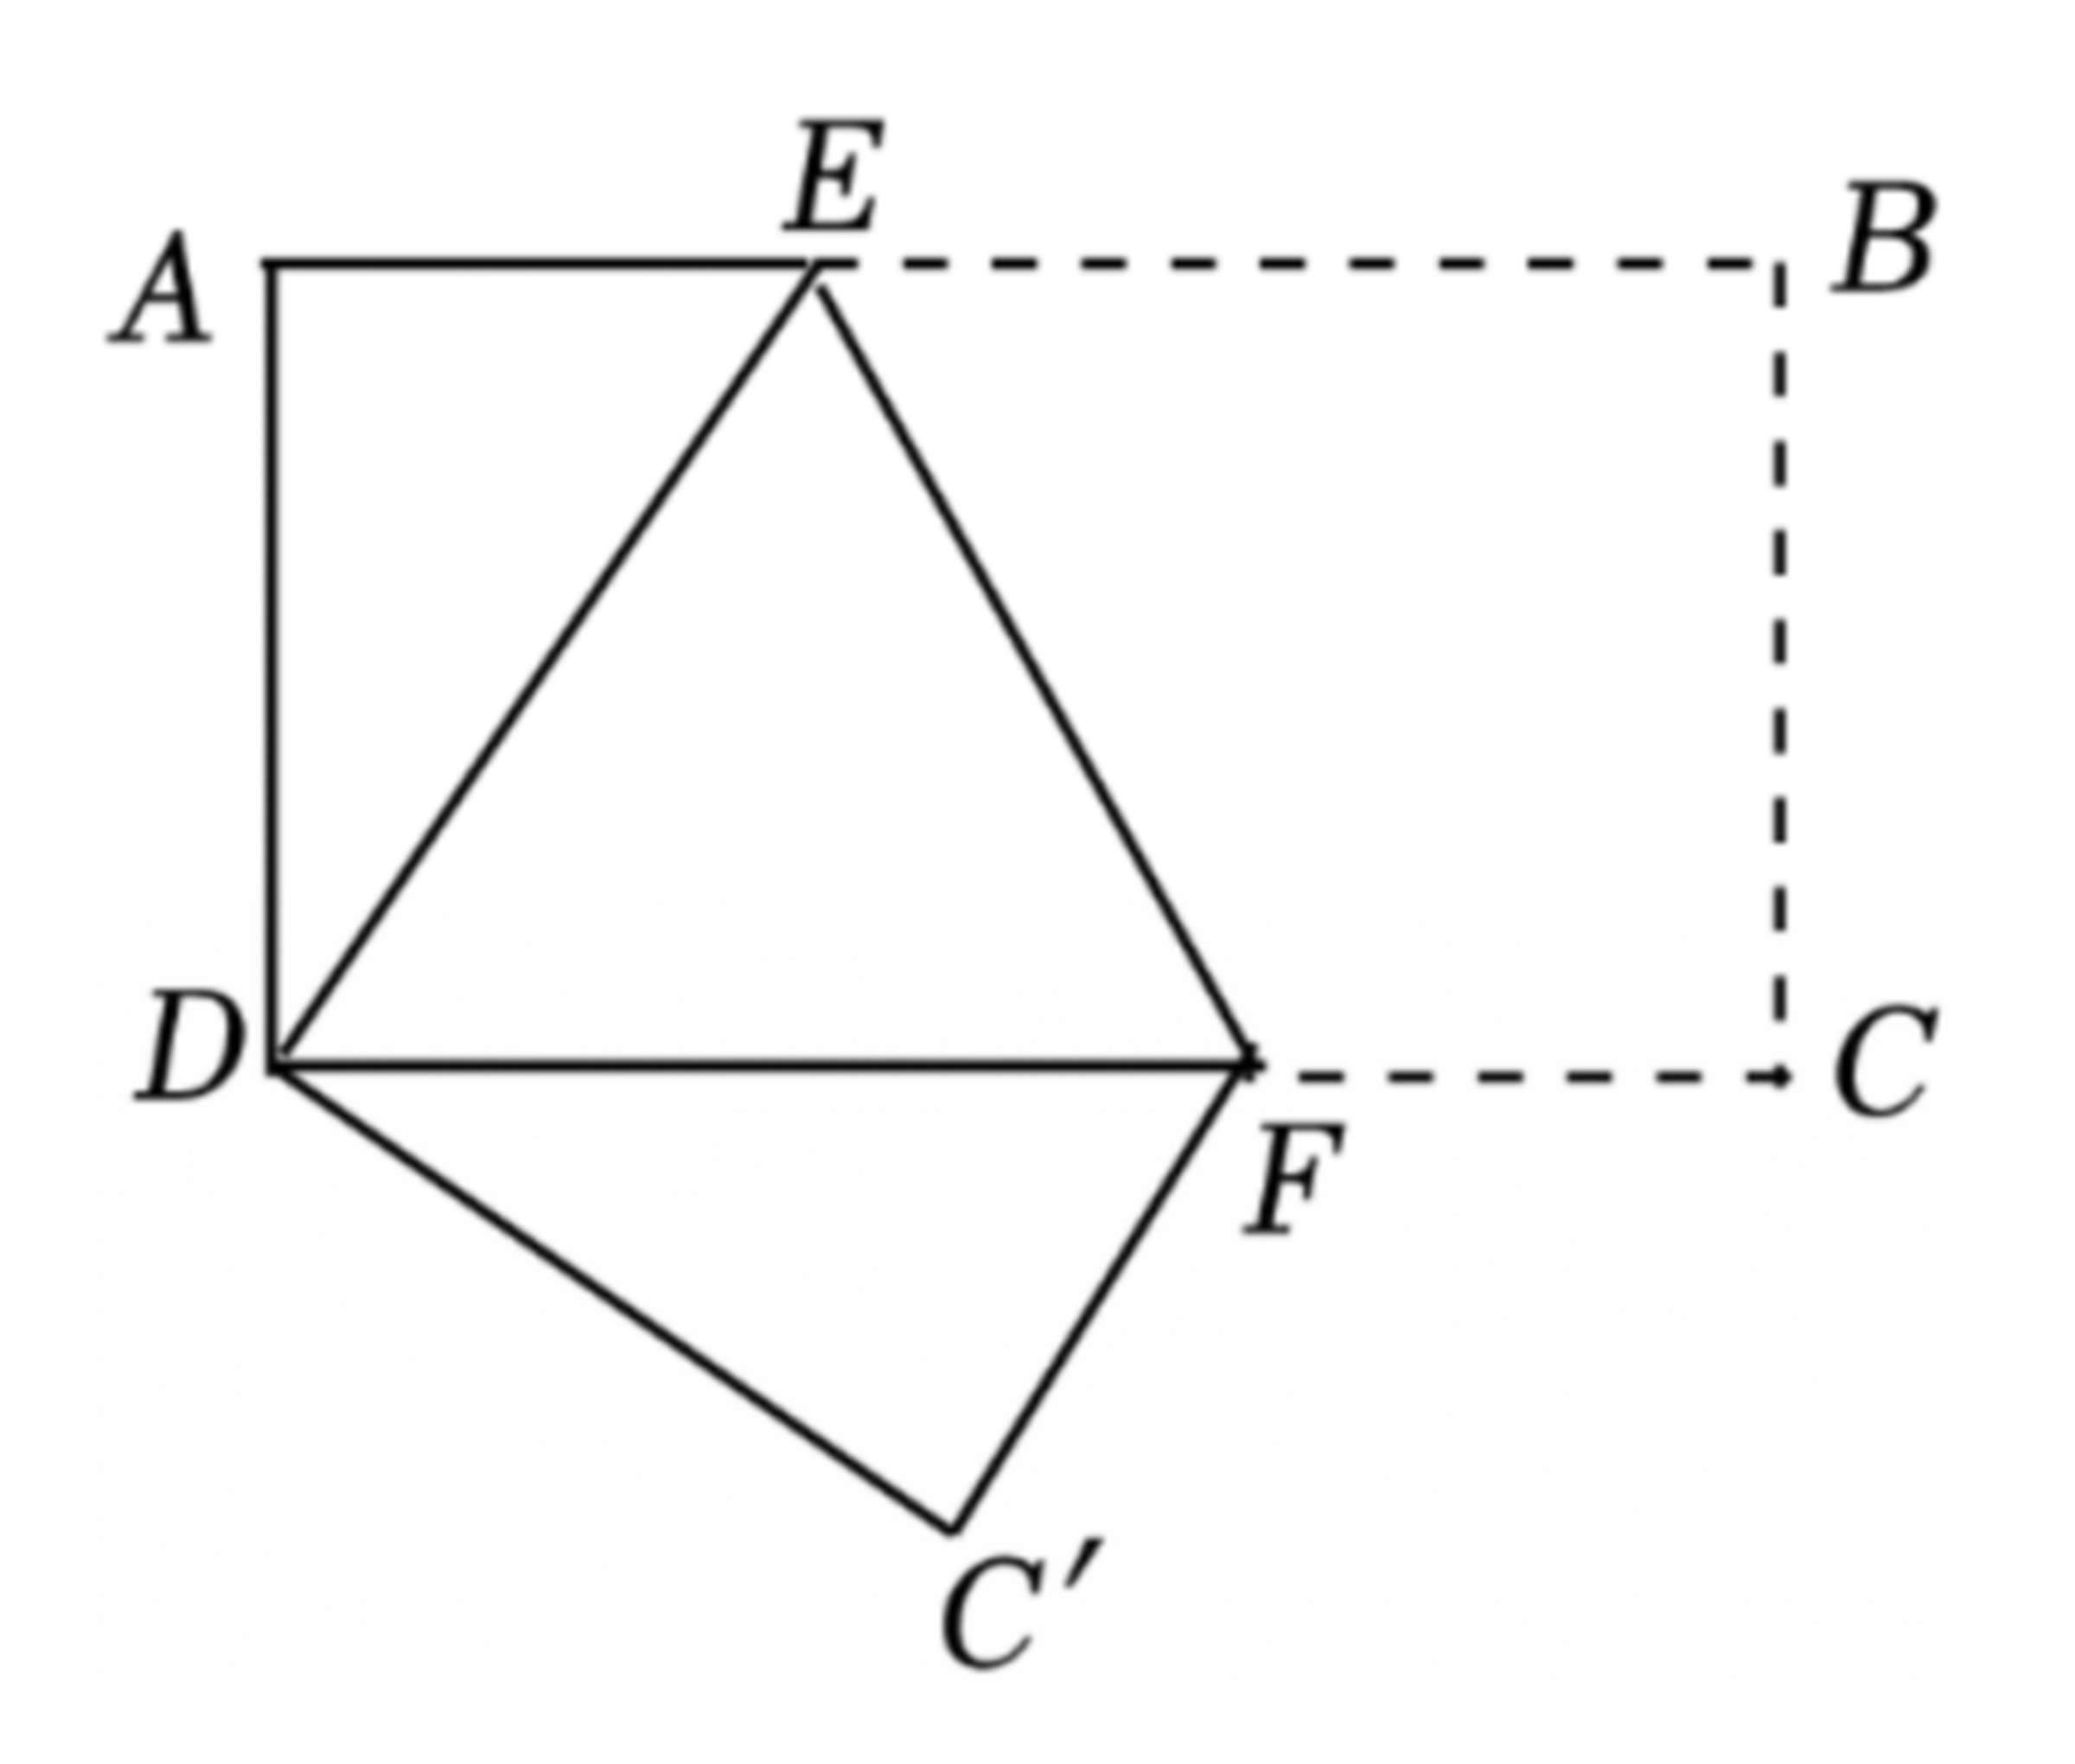
\includegraphics[width=0.40\textwidth]{figures/gao149_q11.png}
\end{center}

\ifanswer
\solbegin
\step{因为矩形 $ABCD(AB>AD)$ 的周长为 12，}
\step{在 $AB$ 和 $CD$ 边上分别取点 $E$ 和 $F$，将四边形 $BCFE$ 沿 $EF$ 折叠，}
\step{使点 $B$ 与点 $D$ 重合，此时点 $C$ 的对应点为 $C'$，}
\step{所以设 $AD=a$，$AB=b$，则 $2(a+b)=12$，}
\step{所以 $a+b=6$，且 $AB>AD$，所以 $b>a>0$，}
\step{设 $DF=x$，则 $C'F=b-x$，在 $Rt\triangle DC'F$ 中，$DC'=BC=a$，}% 几何三角形符号原卷印扁等边细线三角 $\triangle$，照录（放大 02 页确认）；$Rt$ 照录
\step{所以 $a^2+(b-x)^2=x^2$，解得 $x=\dfrac{a^2+b^2}{2b}$，}
\step{因此 $\triangle C'DF$ 的面积 $S=\dfrac{1}{2}\cdot DC'\cdot C'F=\dfrac{1}{2}\cdot a\cdot(b-x)$，}
\step{又 $b-x=b-\dfrac{(6-b)^2+b^2}{2b}=\dfrac{6(b-3)}{b}$，}
\step{所以 $S=\dfrac{1}{2}\cdot a\cdot\dfrac{6(b-3)}{b}=\dfrac{1}{2}\cdot(6-b)\cdot\dfrac{6(b-3)}{b}=\dfrac{3(6-b)(b-3)}{b}$}
\step{$=3\cdot\left(-b-\dfrac{18}{b}+9\right)$，又 $b+\dfrac{18}{b}\geqslant2\sqrt{b\cdot\dfrac{18}{b}}=6\sqrt{2}$，}
\step{当且仅当 $b=\dfrac{18}{b}$ 即 $b=3\sqrt{2}$ 时取等号，此时满足 $b>a$，}
\step{所以 $S\leqslant3\cdot(-6\sqrt{2}+9)=27-18\sqrt{2}$，故 $\triangle C'DF$ 面积的最大值为 $27-18\sqrt{2}$.}
\solend
\fi

% === Q12 === 解析内 3 幅三次函数曲线坐标图（仅答案版出）；解析 15 行（8 行 03 页＋7 行 04 页）
\item 已知 $m>0$，若存在 $t\in\R$，使得对任意 $x\in[0,m]$，不等式 $[(x-1)^2-t](x-t)\leqslant0$ 恒成立，则 $m$ 的最大值是\blankline[4.4em].

\ifanswer
\solbegin
\step{当 $t\leqslant0$ 时，$(x-1)^2-t\geqslant0$ 恒成立，}
\step{不等式 $[(x-1)^2-t](x-t)\leqslant0$ 的解集为 $x\leqslant t$，与 $x\in[0,m]$ 矛盾；}
\step{当 $t>0$ 时，不等式 $[(x-1)^2-t](x-t)\leqslant0\Leftrightarrow(x-1-\sqrt t)(x-1+\sqrt t)(x-t)\leqslant0$，}
\step{若 $t<1-\sqrt t$，即 $t\in\left(0,\dfrac{3-\sqrt5}{2}\right)$，}
\begin{center}
% 情形一 $t<1-\sqrt t$ 曲线图取 03 页右侧，去粉色水印、去色、4× LANCZOS 放大；仅答案版出
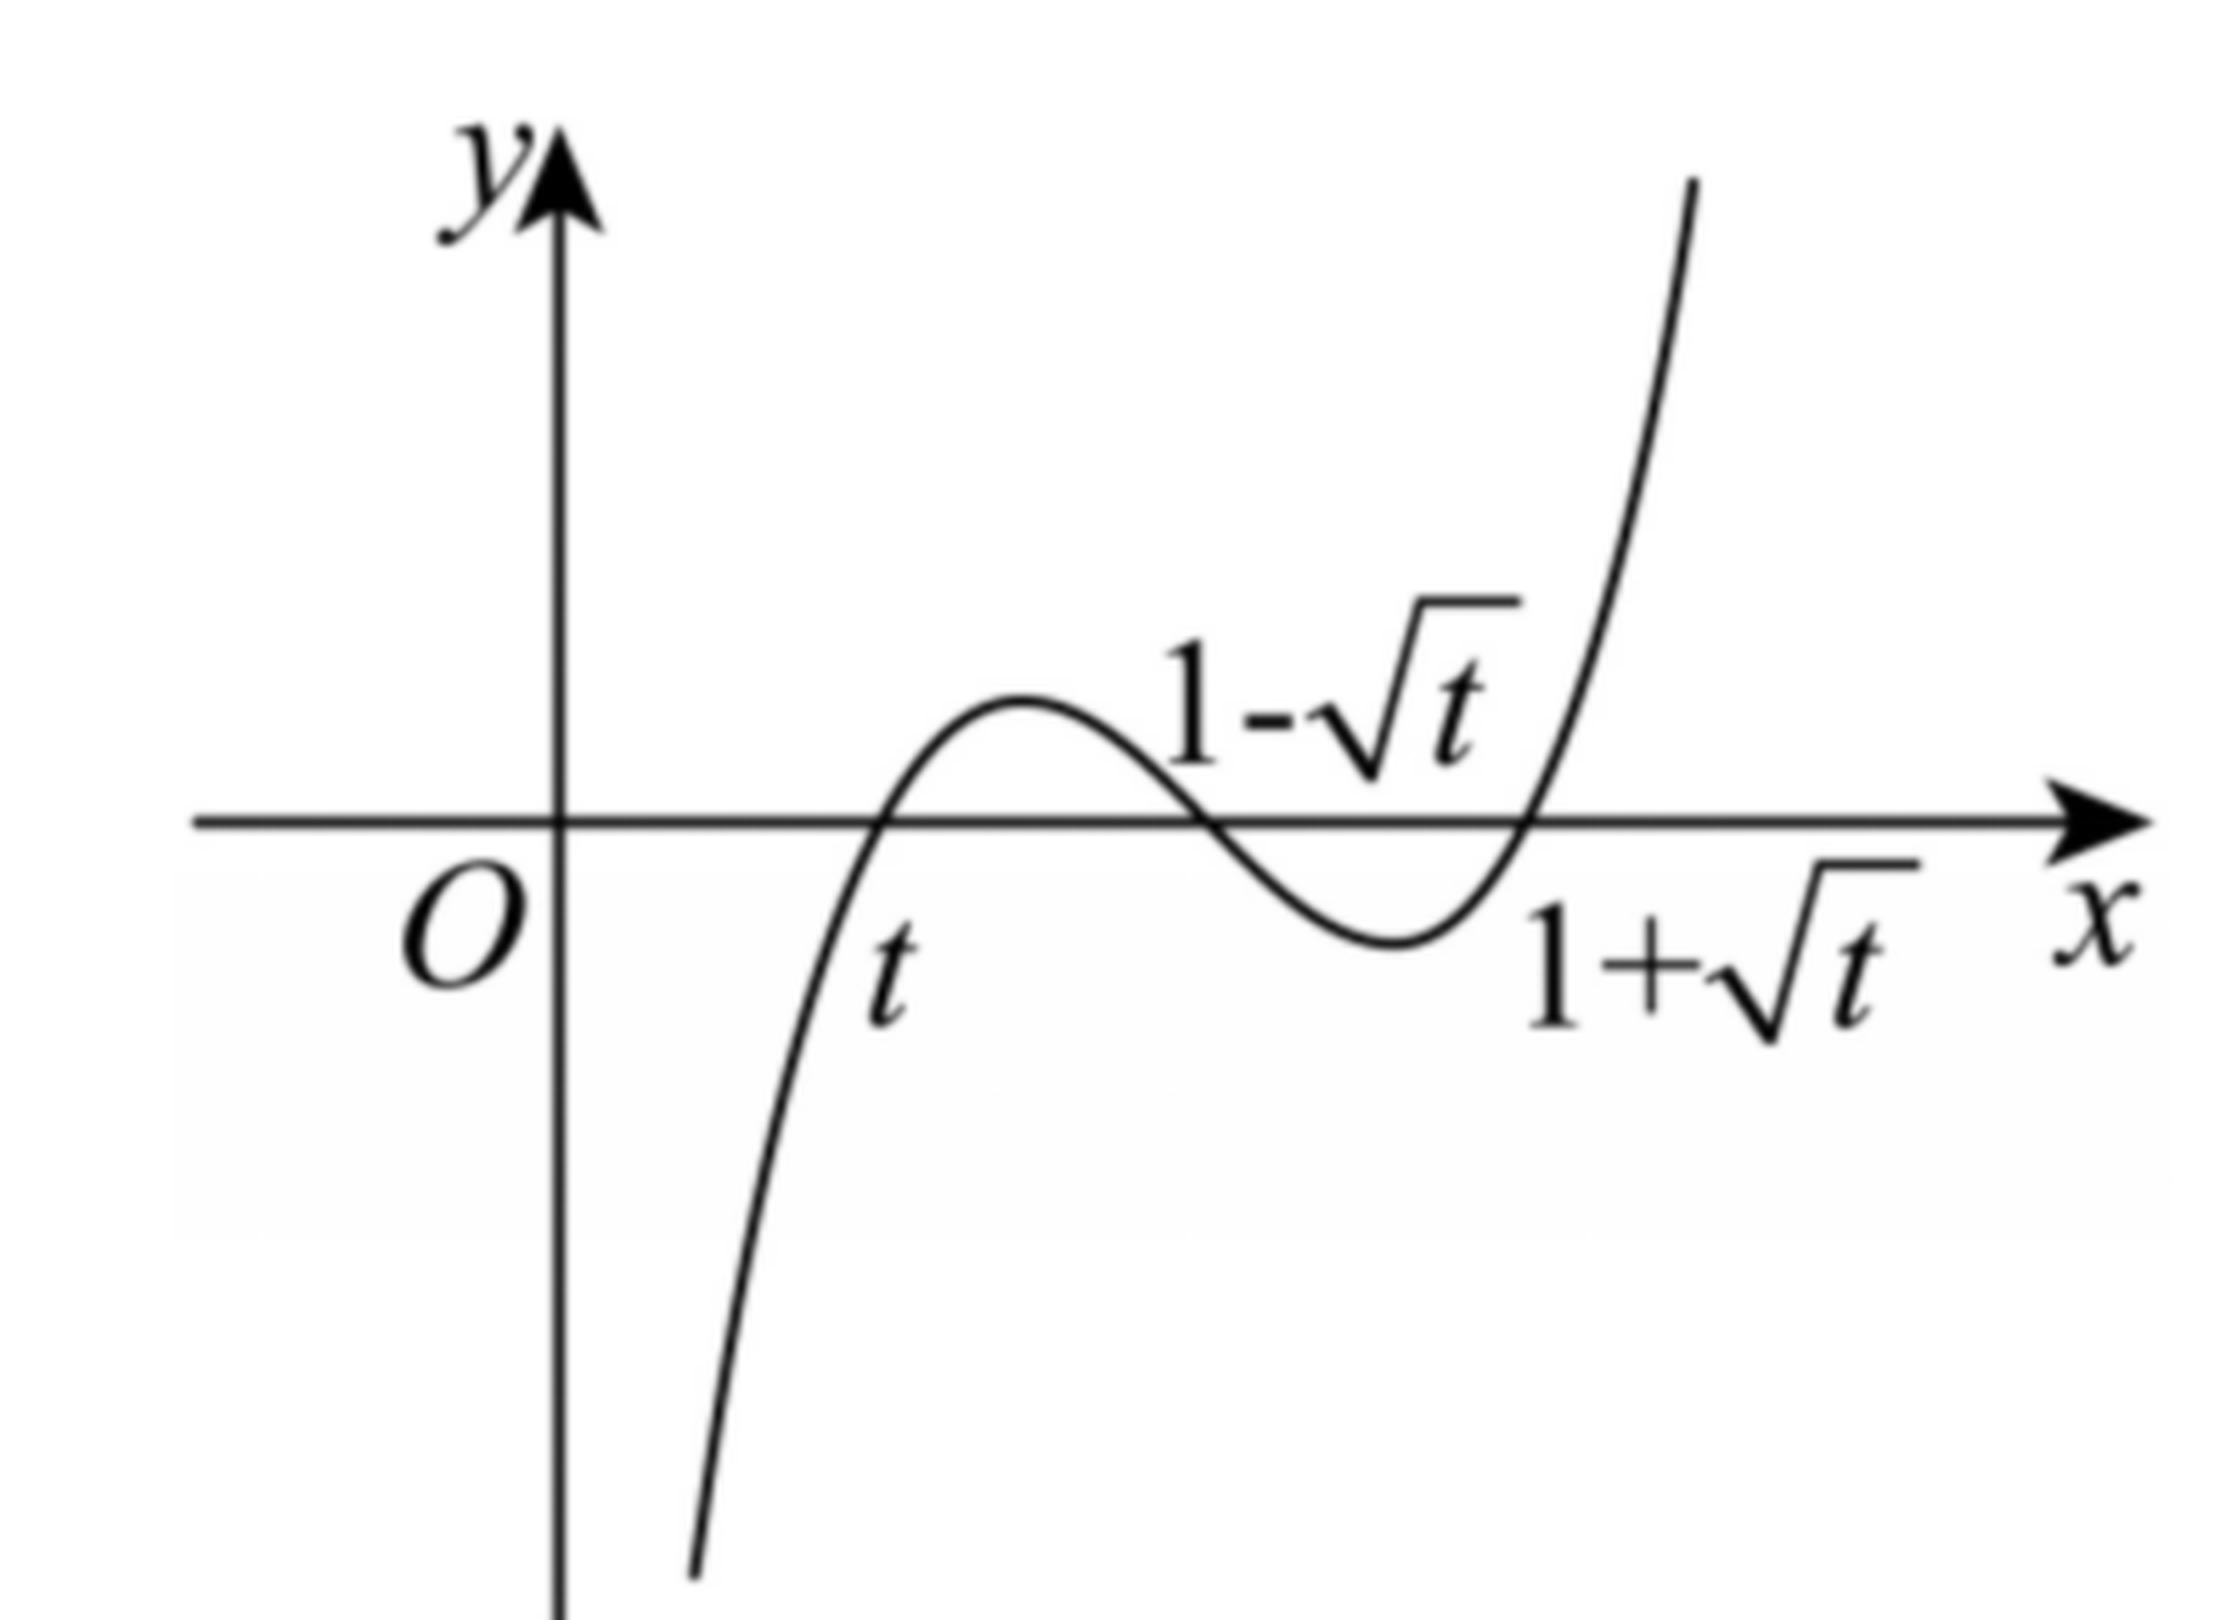
\includegraphics[width=0.40\textwidth]{figures/gao149_q12_a.png}
\end{center}
\step{则原不等式的解集为 $(-\infty,t]\cup[1-\sqrt t,1+\sqrt t]$，}
\step{当 $0<m\leqslant t$ 时，原不等式恒成立，因此}
\step{$m\in\left(0,\dfrac{3-\sqrt5}{2}\right)$；}
\step{若 $t=1-\sqrt t$，即 $t=\dfrac{3-\sqrt5}{2}$，则原不等式的解集为 $(-\infty,1+\sqrt t]$，}
\begin{center}
% 情形二 $t=1-\sqrt t$ 曲线图取 03 页右侧，去粉色水印、去色、4× LANCZOS 放大；仅答案版出
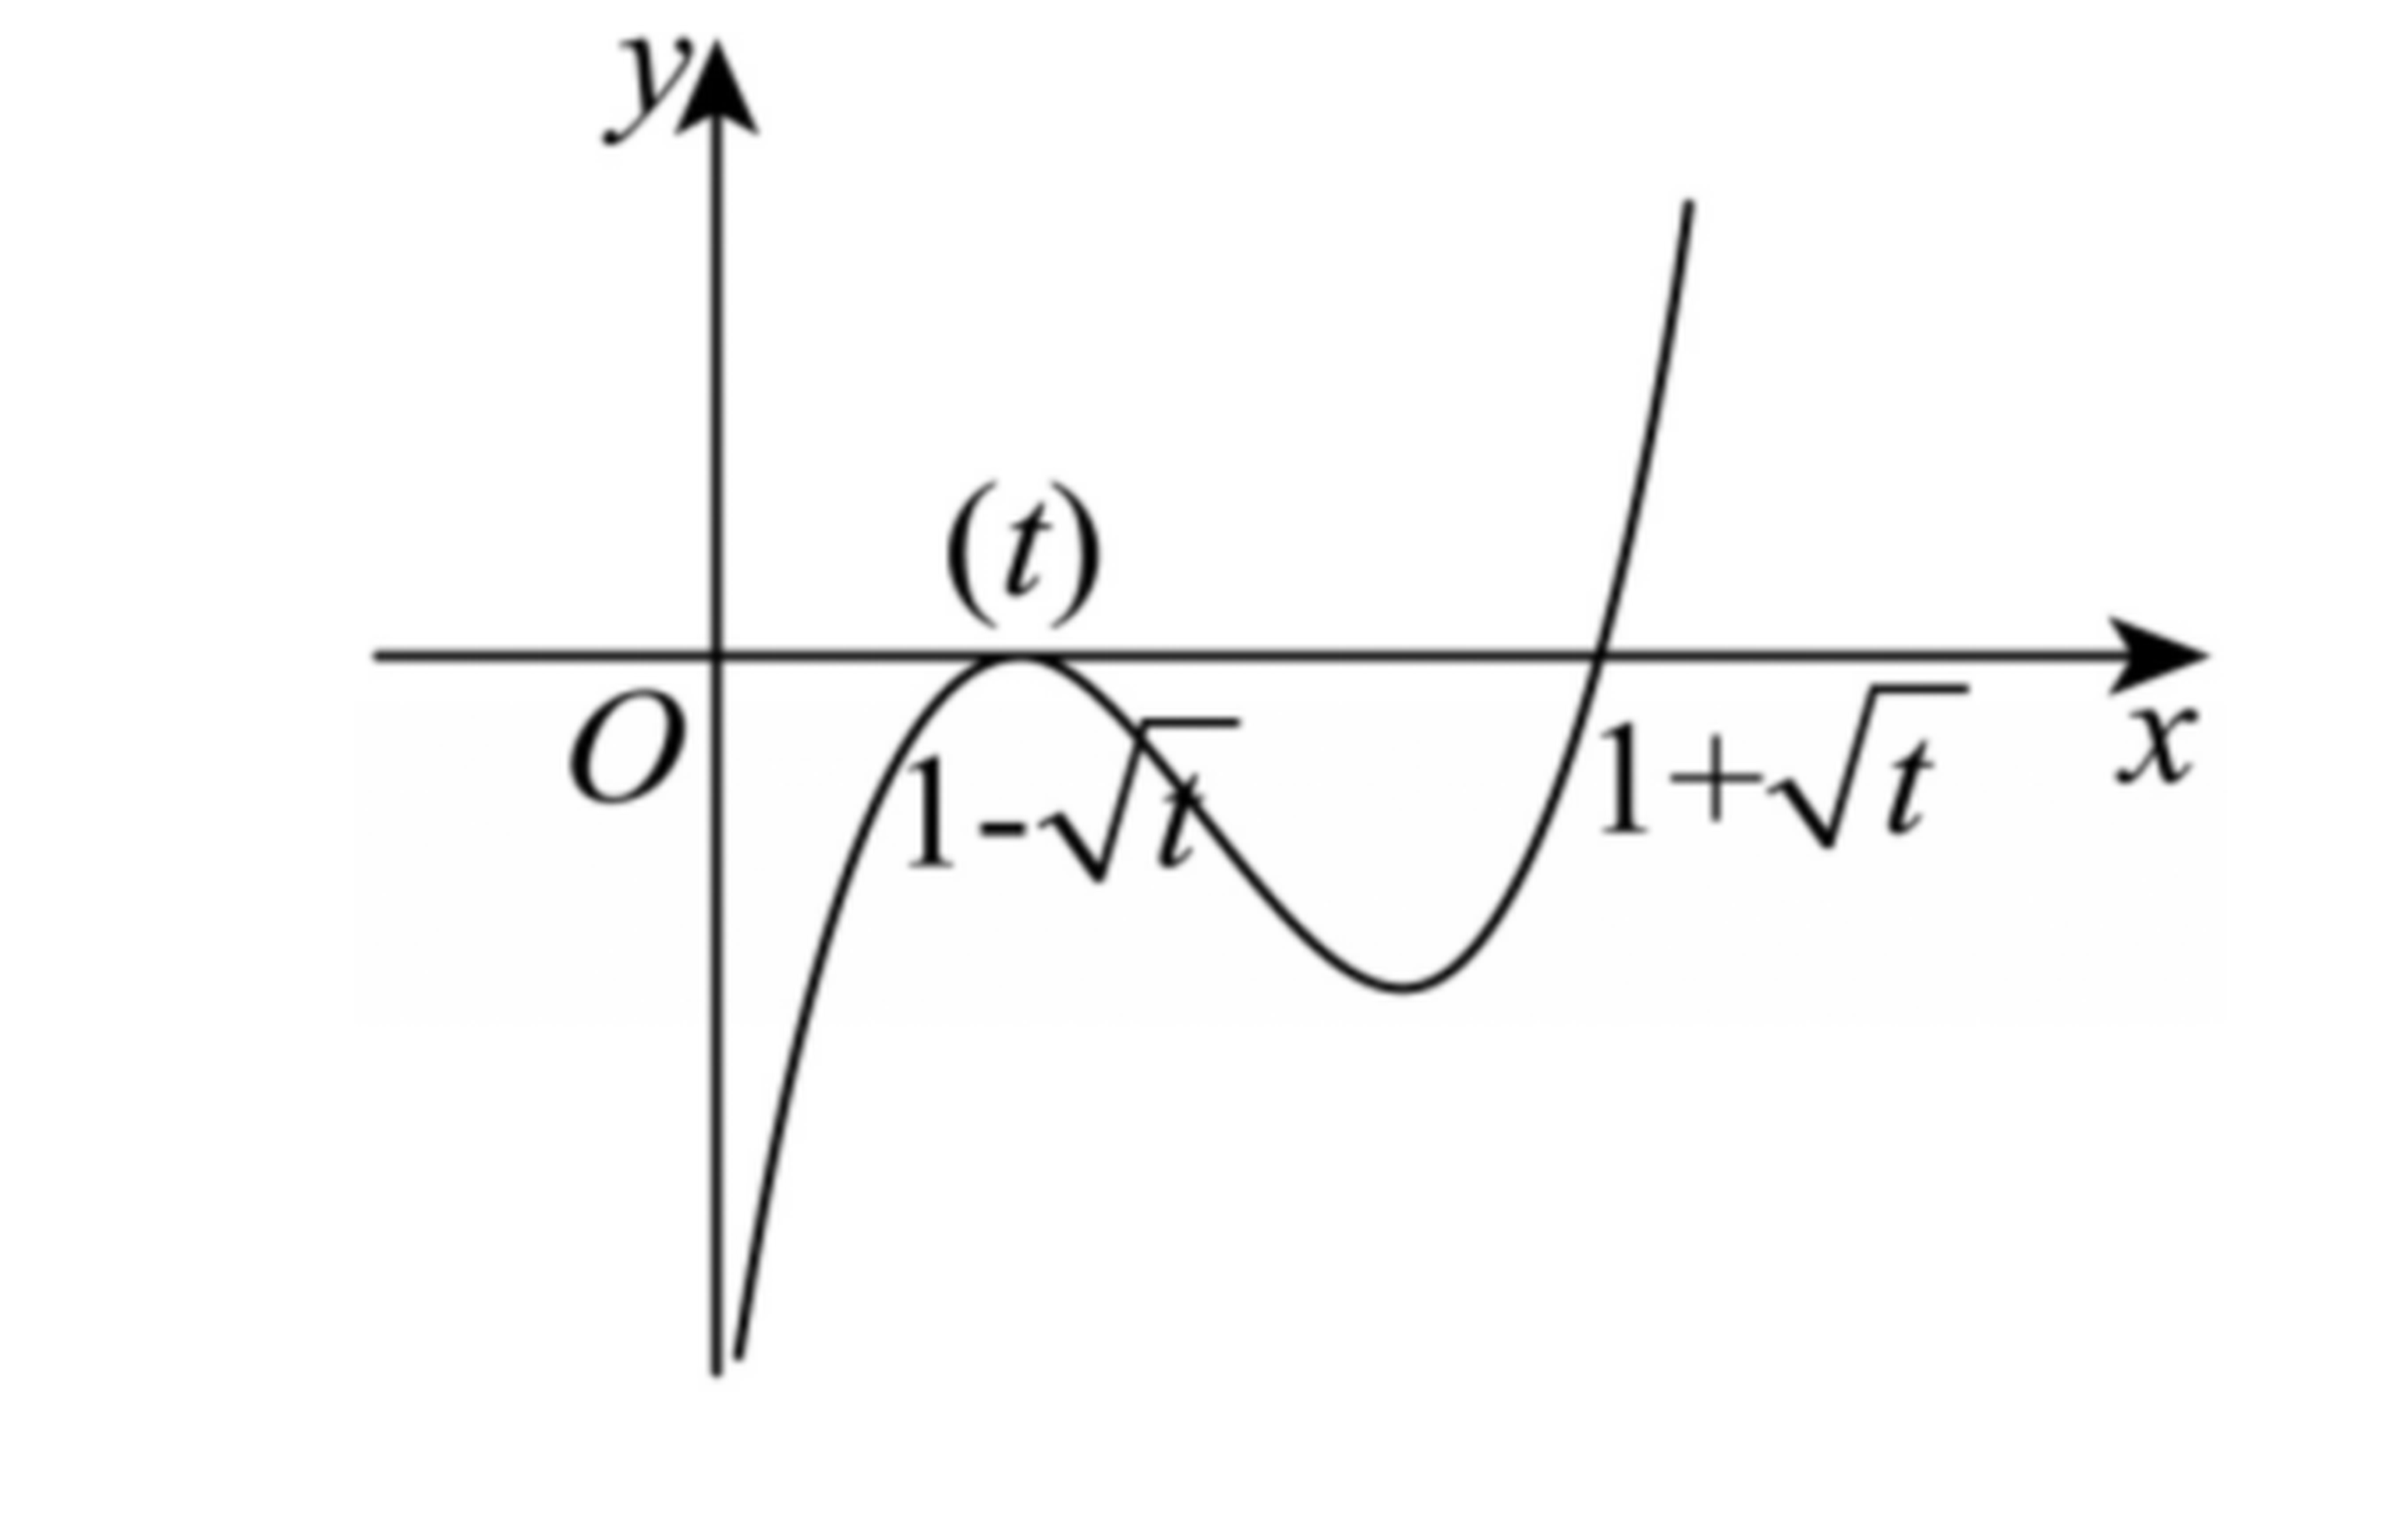
\includegraphics[width=0.40\textwidth]{figures/gao149_q12_b.png}
\end{center}
\step{当 $0<m\leqslant1+\sqrt t$ 时，原不等式恒成立，因此 $m\in\left(0,\dfrac{\sqrt5+1}{2}\right]$；}
\step{若 $1+\sqrt t>t>1-\sqrt t$，即 $t\in\left(\dfrac{3-\sqrt5}{2},\dfrac{3+\sqrt5}{2}\right)$，}
\begin{center}
% 情形三 $1+\sqrt t>t>1-\sqrt t$ 曲线图取 04 页右侧，去粉色水印、去色、4× LANCZOS 放大；仅答案版出
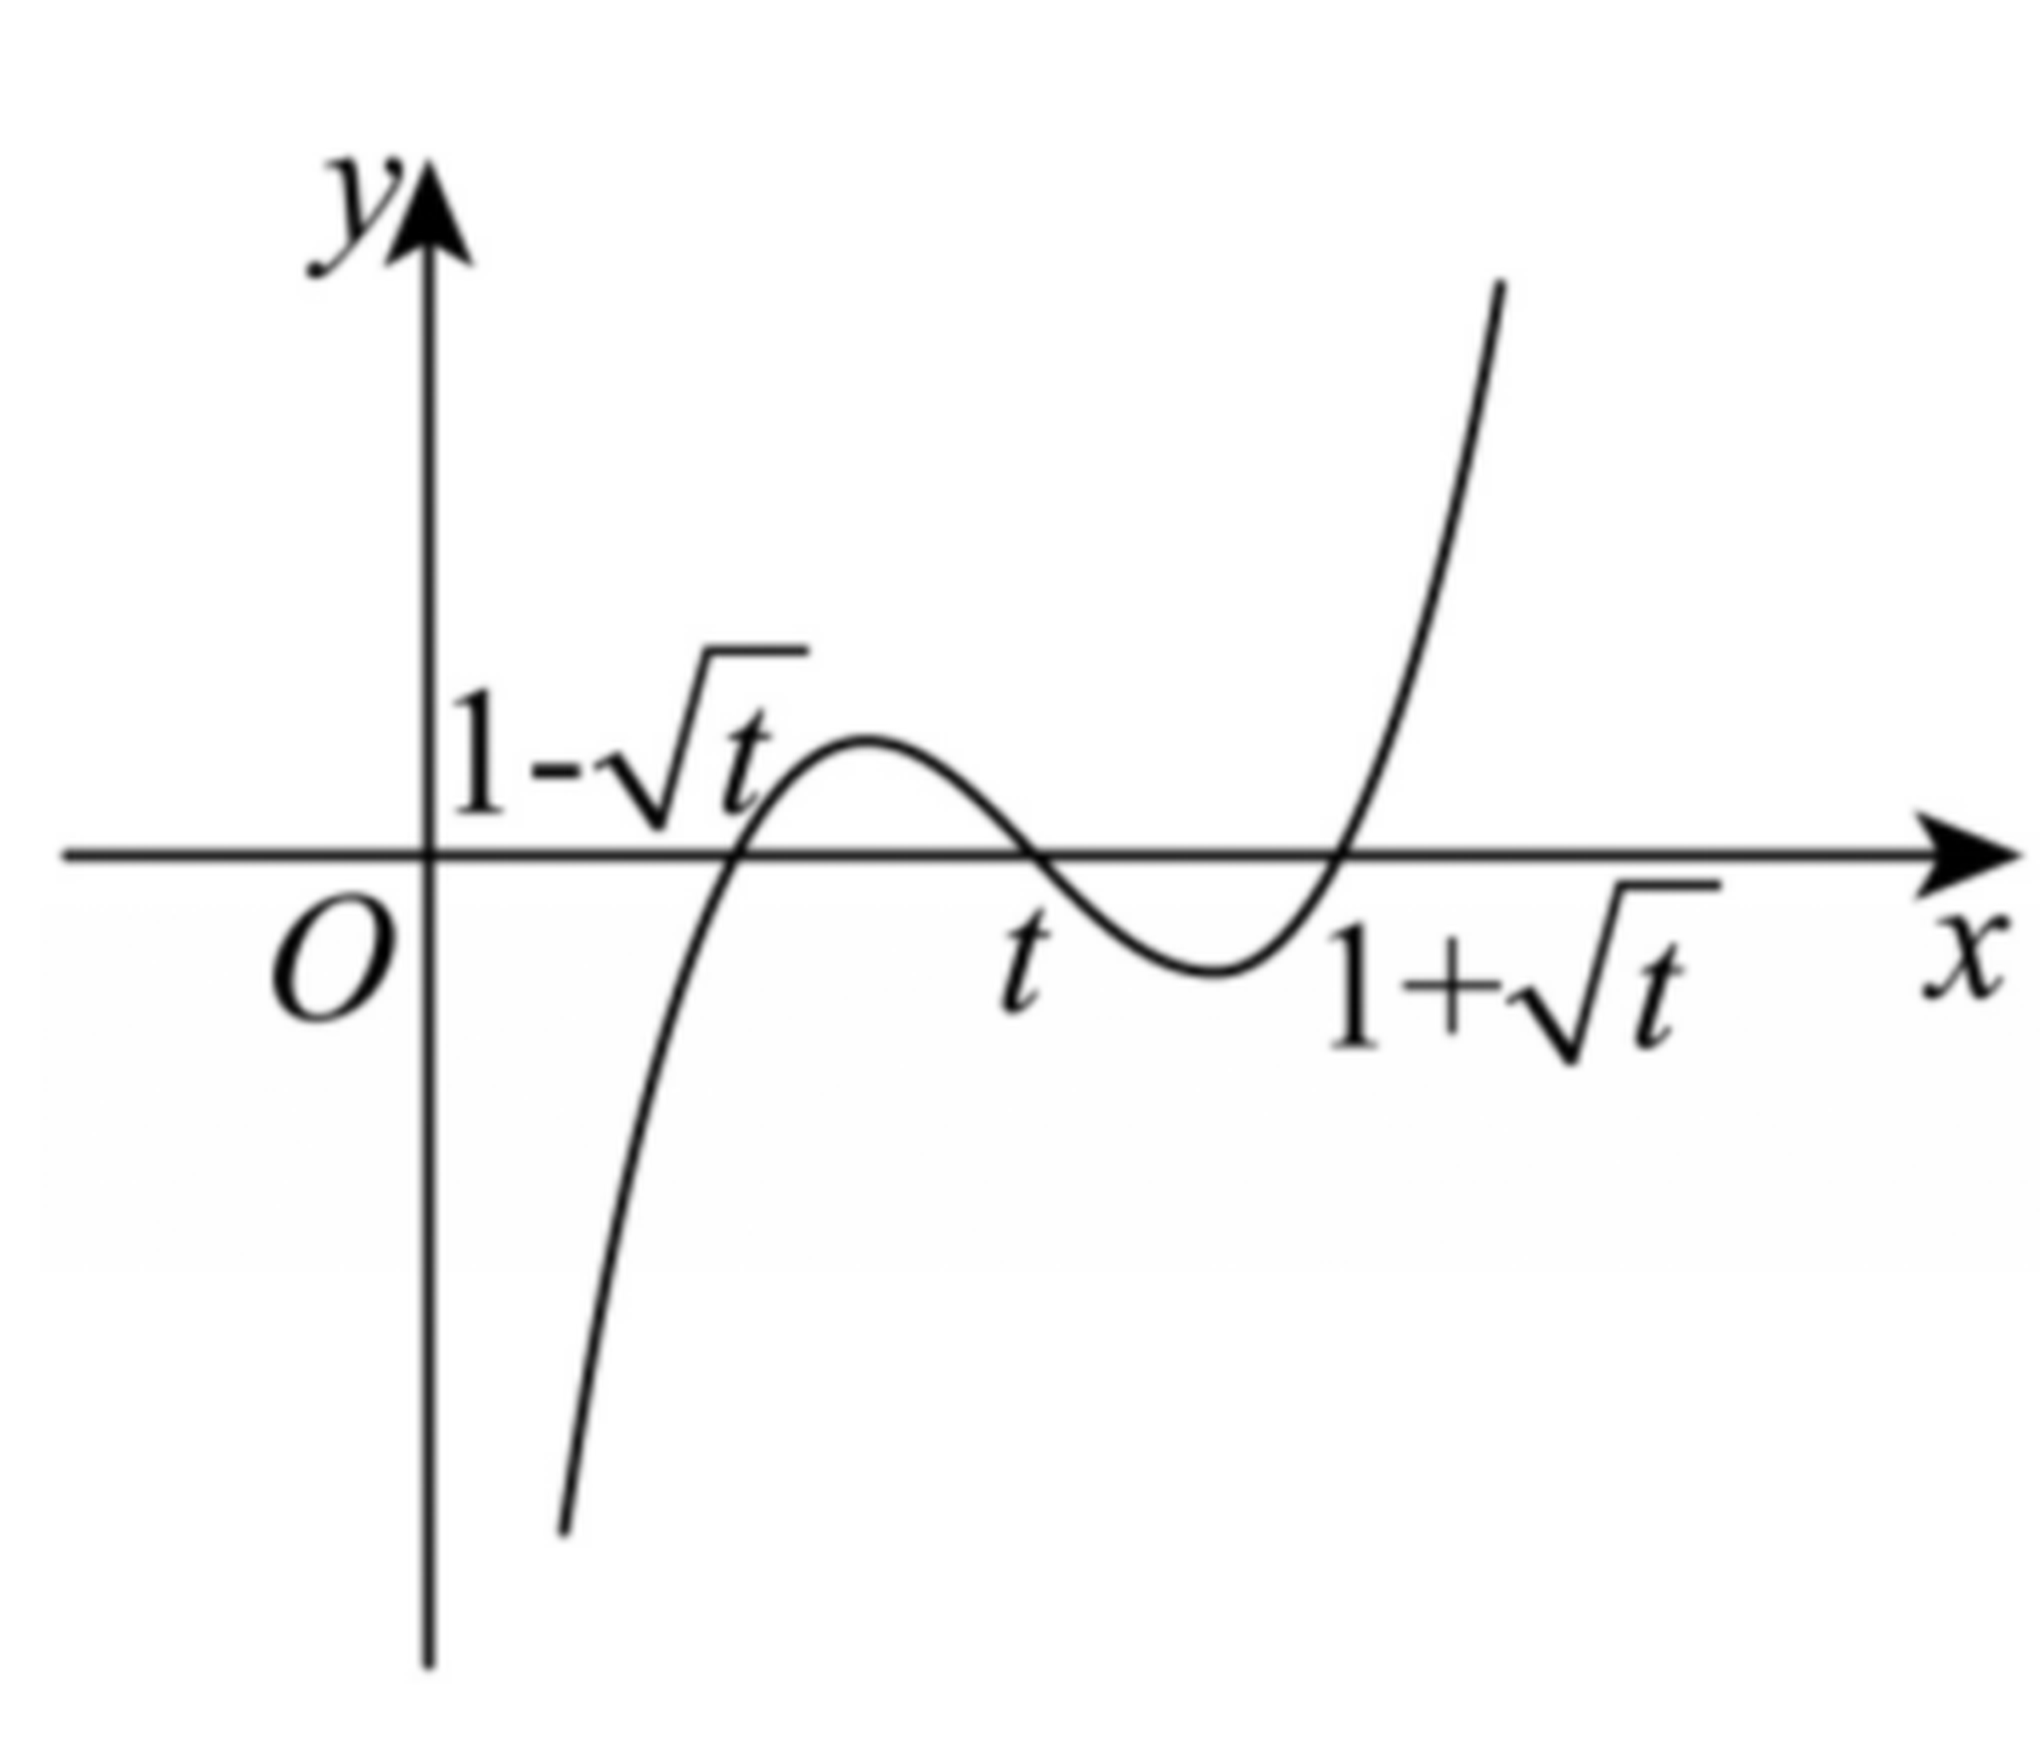
\includegraphics[width=0.40\textwidth]{figures/gao149_q12_c.png}
\end{center}
\step{则原不等式的解集为 $(-\infty,1-\sqrt t]\cup[t,1+\sqrt t]$，}
\step{当 $\begin{cases}1-\sqrt t>0\\1-\sqrt t\geqslant m\end{cases}$ 时，原不等式恒成立，此时 $t\in\left(\dfrac{3-\sqrt5}{2},1\right)$，$m\in\left(0,\dfrac{3-\sqrt5}{2}\right)$；}
\step{若 $t\geqslant1+\sqrt t$，即 $t\geqslant\dfrac{3+\sqrt5}{2}$，则取 $x=0$，$(t-1)t>0$，}
\step{原不等式不恒成立，不符合题意，}
\step{因此实数 $m$ 的取值范围是 $\left(0,\dfrac{\sqrt5+1}{2}\right]$，$m$ 的最大值是 $\dfrac{\sqrt5+1}{2}$.}
\solend
\fi

\end{enumerate}

\bigsec{二、选择题}

\begin{enumerate}
\setcounter{enumi}{12}

% === Q13 ===：答案"C"直接印在题干括号内、无【答案】/【解析】段，按 高一84 Q13／高一148 Q13 成例括号留空、另提 \ans{$C$}；四选项两行两列照原卷分行
\item 设 $ab>0$，则 $a>b$ 是 $\dfrac{1}{a}<\dfrac{1}{b}$ 的\mbox{（\quad）}

\keepwithprev
A. 充分不必要条件\qquad\qquad B. 必要不充分条件

C. 充要条件\qquad\qquad D. 既不充分又不必要条件

\ifanswer
\ans{$C$}
\fi

% === Q14 ===：$A\subset B$ 单线照录；四选项补集照原卷上划线 \overline{A}／\overline{B}；解析 1 行（由韦恩图得 B 对）
\item 已知集合 $A$、$B$ 非空，且 $A\subset B$，则下列式子中一定是空集的为\mbox{（\quad）}

\keepwithprev
A. $\overline{A}\cap B$\qquad B. $A\cap\overline{B}$\qquad C. $\overline{A}\cap\overline{B}$\qquad D. $\overline{A}\cup\overline{B}$

\ifanswer
\solbegin
\step{由韦恩图得 $B$ 对. 故选 $B$.}
\solend
\fi

% === Q15 ===："天文数字"弯引号照录；解析 2 行（首行在 04 页末、末行续 05 页顶）
\item 历史上数学计算方面的三大发明是阿拉伯数字、十进制和对数，其中对数的发明，大大缩短了计算时间，为人类研究科学和了解自然起了重大作用，对数运算对估算“天文数字”具有独特的优势. $2.5^{1000}$ 的估算值约为\mbox{（\quad）}

\keepwithprev
A. $10^{365}$\qquad B. $10^{379}$\qquad C. $10^{389}$\qquad D. $10^{398}$

\ifanswer
\solbegin
\step{$\lg 2.5^{1000}=1000\lg 2.5=1000(1-2\lg 2)\approx1000\times(1-0.602)=398$，}
\step{所以 $2.5^{1000}\approx10^{398}$. 故选 $D$.}
\solend
\fi

% === Q16 ===："完美集"新定义、圈数字①②文本模式；题干"若对任意 $x$，$y\in A$"用全角逗号、解析用顿号"$x$、$y\in A$"，两处照录不统一；解析 9 行
\item 设全集 $U=\R$，集合 $A$ 是一个非空数集，若对任意 $x$，$y\in A$，都有 $x+y\in A$、$xy\in A$，则称集合 $A$ 为一个“完美集”，给出以下命题：

①若 $A_1$、$A_2$ 都是“完美集”，且 $A_1\cap A_2\ne\varnothing$，则 $A_1\cap A_2$ 也是“完美集”；

②若 $A_1$、$A_2$ 都是“完美集”，则 $A_1\cup A_2$ 也是“完美集”.

下列说法正确的是\mbox{（\quad）}

\keepwithprev
A. ①②都是真命题\qquad\qquad B. ①是真命题，②是假命题

C. ①是假命题，②是真命题\qquad\qquad D. ①②都是假命题

\ifanswer
\solbegin
\step{由题意，全集 $U=\R$，集合 $A$ 是一个非空数集，}
\step{若对任意 $x$、$y\in A$，都有 $x+y\in A$、$xy\in A$，则称集合 $A$ 为一个“完美集”，}
\step{对于①，取 $x$、$y\in A_1\cap A_2$，则 $x\in A_1$，$x\in A_2$，$y\in A_1$，$y\in A_2$，}
\step{又 $A_1$、$A_2$ 是“完美集”，所以 $x+y\in A_1$，$xy\in A_1$，$x+y\in A_2$，$xy\in A_2$，}
\step{所以 $x+y\in A_1\cap A_2$，$xy\in A_1\cap A_2$，所以 $A_1\cap A_2$ 是“完美集”，故①正确；}
\step{对于②，取“完美集” $A_1=\{x\mid x=2k,k\in\Z\}$，$A_2=\{x\mid x=3k,k\in\Z\}$，}
\step{则 $2\in A_1$，$3\in A_2$，但 $2+3\notin A_1\cup A_2$，}
\step{即此时 $A_1\cup A_2$ 不是“完美集”，故②错误.}
\step{故选 $B$.}
\solend
\fi
\end{enumerate}

\bigsec{三、解答题}

\begin{enumerate}
\setcounter{enumi}{16}

% === Q17 ===："图像"（有亻）照录（Q17 题干与解析共 2 处）；绝对值 \lvert…\rvert；解析 7 行
\item 已知 $m\in\R$，$f(x)=(m^2-m-5)x^m$. 若 $y=f(x)$ 是幂函数，且其图像不经过原点.

(1) 求实数 $m$ 的值；

(2) 若 $f(a)=f(b)$ 且 $a\ne b$，求 $\lvert a+2\rvert+\lvert b-1\rvert$ 的最小值，并指出取到最小值时 $a$ 的取值范围.

\ifanswer
\solbegin
\step{(1) $f(x)=(m^2-m-5)x^m$ 是幂函数，得 $m^2-m-5=1$，即 $m^2-m-6=0$，}
\step{解得 $m=-2$ 或 $m=3$，又函数图像不经过原点，所以 $m=-2$($3$ 舍)；}
\step{(2) 由 (1) 得 $f(x)=x^{-2}=\dfrac{1}{x^2}$ 为偶函数，}
\step{$x<0$ 时，函数 $f(x)$ 严格增，$x>0$ 时，函数 $f(x)$ 严格减，}
\step{又 $f(a)=f(b)$ 且 $a\ne b$，所以 $a=-b$，且 $a\ne0$，$b\ne0$，}
\step{则 $\lvert a+2\rvert+\lvert b-1\rvert=\lvert a+2\rvert+\lvert-a-1\rvert=\lvert a+2\rvert+\lvert a+1\rvert$，}
\step{则 $\lvert a+2\rvert+\lvert b-1\rvert$ 的最小值为 $1$，取到最小值时 $a$ 的取值范围是 $[-2,-1]$.}
\solend
\fi

% === Q18 ===：判别式两形混用——(1) cases 块印高 \Delta、(2) 独立行印扁 \triangle，逐处照录不统一；解析 8 行
\item 已知命题 $p$：方程 $x^2+4x+m-1=0$ 有两个不等的负根；命题 $q$：方程 $4x^2+4x+m-2=0$ 无实根.

(1) 若 $p$ 为真命题，求 $m$ 的取值范围；

(2) 若 $p$、$q$ 两命题一真一假，求 $m$ 的取值范围.

\ifanswer
\solbegin
\step{(1) 若 $p$ 为真命题，即方程 $x^2+4x+m-1=0$ 有两个不等的负根；}
\step{必有 $\begin{cases}\Delta=16-4(m-1)>0\\m-1>0\end{cases}$，解得 $1<m<5$，即 $m$ 的取值范围为 $(1,5)$；}
\step{(2) 命题 $q$：方程 $4x^2+4x+m-2=0$ 无实根，}
\step{则有 $\triangle=16-16(m-2)<0$，解得 $m>3$，}
\step{若 $p$ 和 $q$ 有且只有一个为真命题，}
\step{若 $p$ 真 $q$ 假，必有 $\begin{cases}1<m<5\\m\leqslant3\end{cases}$，则有 $1<m\leqslant3$，}
\step{若 $p$ 假 $q$ 真，必有 $\begin{cases}m\leqslant1\text{ 或 }m\geqslant5\\m>3\end{cases}$，则有 $m\geqslant5$，}
\step{综上，$1<m\leqslant3$ 或 $m\geqslant5$.}
\solend
\fi

% === Q19 ===：$A\subseteq B$ 带下划线照录；解析 7 行（(2) 两组 cases 并排）
\item 已知 $m\in\R$，集合 $A=\left\{x\mid y=\sqrt{3-x}-\dfrac{1}{\sqrt{x-1}}\right\}$，集合 $B=\{x\mid 2m\leqslant x\leqslant1-m\}$.

(1) 若 $A\cup B=B$，求实数 $m$ 的取值范围；

(2) 若 $A\cap B=\varnothing$，求实数 $m$ 的取值范围.

\ifanswer
\solbegin
\step{(1) 函数 $y=\sqrt{3-x}-\dfrac{1}{\sqrt{x-1}}$，则 $\begin{cases}3-x\geqslant0\\x-1>0\end{cases}$，解得 $1<x\leqslant3$，}
\step{所以 $A=\{x\mid1<x\leqslant3\}$，}
\step{因为 $A\cup B=B$，所以 $A\subseteq B$，则 $\begin{cases}2m\leqslant1\\1-m\geqslant3\end{cases}$，解得 $m\leqslant-2$，}
\step{综上，实数 $m$ 的取值范围为 $(-\infty,-2]$；}
\step{(2) 当 $B=\varnothing$ 时，则 $2m>1-m$，解得 $m>\dfrac{1}{3}$，}
\step{当 $B\ne\varnothing$ 时，则 $\begin{cases}2m\leqslant1-m\\2m>3\end{cases}$ 或 $\begin{cases}2m\leqslant1-m\\1-m\leqslant1\end{cases}$，解得 $m\in\varnothing$ 或 $0\leqslant m\leqslant\dfrac{1}{3}$，}
\step{综上，实数 $m$ 的取值范围为 $[0,+\infty)$.}
\solend
\fi

% === Q20 ===：n 阶基本不等式推广；(3) 解析含 \overbrace{…}^{k} 上括号；(2) 解析"x=x=x=3(1-x)"三连等系原卷笔误、照录加注（见 ⑤）；解析 14 行
\item 教材中的基本不等式可以推广到 $n$ 阶：$n$ 个正数的算术平均数不小于它们的几何平均数，即对于任意的正数 $a_1$、$a_2$、$\cdots$、$a_n$，有 $\dfrac{a_1+a_2+\cdots+a_n}{n}\geqslant\sqrt[n]{a_1\cdot a_2\cdots a_n}$（$n\in\N$ 且 $n\geqslant2$），且等号当且仅当 $a_1=a_2=\cdots=a_n$ 时成立. 利用此结论解决下列问题：

(1) 若 $x$、$y$、$z>0$，求 $\dfrac{y}{x}+\dfrac{2z}{y}+\dfrac{4x}{z}$ 的最小值；

(2) 已知 $0<x<1$，求 $x^3(1-x)$ 的最大值，并求取得最大值时的 $x$ 的值；

(3) 对任意的正整数 $k$，判断 $\left(1+\dfrac{1}{k}\right)^k$ 与 $\left(1+\dfrac{1}{k+1}\right)^{k+1}$ 的大小关系，并证明.

\ifanswer
\solbegin
\step{(1) 因为 $x$、$y$、$z>0$，有 $\dfrac{y}{x}>0$，$\dfrac{2z}{y}>0$，$\dfrac{4x}{z}>0$}
\step{所以 $\dfrac{y}{x}+\dfrac{2z}{y}+\dfrac{4x}{z}\geqslant3\sqrt[3]{\dfrac{y}{x}\cdot\dfrac{2z}{y}\cdot\dfrac{4x}{z}}=3\sqrt[3]{8}=6$，}
\step{当且仅当 $\dfrac{y}{x}=\dfrac{2z}{y}=\dfrac{4x}{z}$ 时取等号，故 $\dfrac{y}{x}+\dfrac{2z}{y}+\dfrac{4x}{z}$ 的最小值为 $6$.}
\step{(2) 因为 $0<x<1$，所以 $1-x>0$，}
\step{$x^3(1-x)=\dfrac{1}{3}[x\cdot x\cdot x\cdot3(1-x)]\leqslant\dfrac{1}{3}\left[\dfrac{x+x+x+3(1-x)}{4}\right]^4=\dfrac{1}{3}\times\left(\dfrac{3}{4}\right)^4$}
\step{$=\dfrac{27}{256}$，当且仅当 $x=x=x=3(1-x)$，即 $x=3(1-x)$，$x=\dfrac{3}{4}$ 取等号，}% 原卷"x=x=x=3(1-x)"三连等，疑为四因子相等之误排，放大 08 页确认，照录未改（见 ⑤）
\step{所以 $0<x<1$ 时，$x^3(1-x)$ 的最大值是 $\dfrac{27}{256}$，取最大值时 $x=\dfrac{3}{4}$.}
\step{(3) 对任意 $k\in\N^*$，$\left(1+\dfrac{1}{k}\right)^k<\left(1+\dfrac{1}{k+1}\right)^{k+1}$.}
\step{证明：$\left(1+\dfrac{1}{k}\right)^k=\overbrace{\left(1+\dfrac{1}{k}\right)\cdot\left(1+\dfrac{1}{k}\right)\cdots\left(1+\dfrac{1}{k}\right)}^{k}\times1$}
\step{$\leqslant\left(\dfrac{\overbrace{\left(1+\dfrac{1}{k}\right)+\left(1+\dfrac{1}{k}\right)+\cdots+\left(1+\dfrac{1}{k}\right)}^{k}+1}{k+1}\right)^{k+1}$}
\step{$=\left(\dfrac{\overbrace{(1+1+\cdots+1)}^{k}+\overbrace{\left(\dfrac{1}{k}+\dfrac{1}{k}+\cdots+\dfrac{1}{k}\right)}^{k}+1}{k+1}\right)^{k+1}=\left(\dfrac{k+1+1}{k+1}\right)^{k+1}=\left(1+\dfrac{1}{k+1}\right)^{k+1}$，}
\step{当且仅当 $1+\dfrac{1}{k}=1$ 时取等号，}
\step{但是任意 $k\in\N^*$ 时 $1+\dfrac{1}{k}>1$，所以等号不成立，}
\step{故任意 $k\in\N^*$ 时，$\left(1+\dfrac{1}{k}\right)^k<\left(1+\dfrac{1}{k+1}\right)^{k+1}$.}
\solend
\fi

% === Q21 ===："减 k 集"新定义（引号内 k／数字两侧空格照录）；解析 26 行（续 10 页），含 ⑤ 三处原卷笔误照录
\item 定义：对于给定的整数 $k$，若非空集合 $A$ 满足如下 3 个条件：

① $A$ 是正整数集的子集；② $A\ne\{1\}$；

③对任意正整数 $x,y$，若 $x+y\in A$，则 $xy-k\in A$；则称集合 $A$ 为“减 $k$ 集”.

(1) 判断集合 $A=\{1,2\}$ 是否为“减 $0$ 集”？是否为“减 $1$ 集”？（无需说明理由）

(2) 证明：不存在“减 $2$ 集”；

(3) 是否存在“减 $1$ 集”？如果存在，求出所有“减 $1$ 集”；如果不存在，说明理由.

\ifanswer
\solbegin
\step{(1) 因为 $P\subseteq\N^*$，$P\ne\{1\}$，$1+1=2\in P$，$1\times1-0\in P$，}
\step{所以集合 $P=\{1,2\}$ 是“减 $0$ 集”；}
\step{因为 $P\subseteq\N^*$，$P\ne\{1\}$，$1+1=2\in P$，$1\times1-1\notin P$，}
\step{所以集合 $P=\{1,2\}$ 是“减 $1$ 集”；}% 按条件③应为"不是"，原卷径印"是"，放大 09 页确认，照录未改（见 ⑤）
\step{(2) 假设存在集合 $A$ 是“减 $2$ 集”，若 $x+y\in A$，则 $xy-2\in A$，}
\step{①当 $x+y=xy-2$ 时，有 $(x-1)(y-1)=3$，}
\step{则 $x$、$y$ 一个为 $2$，一个为 $4$，所以集合 $A$ 有元素 $6$，}
\step{但 $3+3\in A$，$3\times3-2\notin A$，与 $A$ 是“减 $2$ 集”矛盾；}
\step{②当 $x+y\ne xy-2$ 时，则 $x+y=xy-1$ 或 $x+y=xy-m$($m>2$)，}
\step{若 $x+y=xy-1$，$m=1$ 时，$M$ 为除 $1$ 以外的最小元素，}% 原卷"m=1"上文未显式定义，疑笔误，放大 09 页确认，照录未改（见 ⑤）
\step{则 $x=M-1$，$y=1$ 时，$xy-2=M-3$ 小于 $M$，}
\step{要符合题意，必须 $M=4$，}
\step{此时取 $x-2$，$y=2$，$xy-2=2$ 不属于 $A$，故不符合题意，}% 原卷"取 x−2"疑为"取 x=2"误排，放大 09 页确认，照录未改（见 ⑤）
\step{当 $m>2$ 时，$(x-1)(y-1)=m+1$，同样得出矛盾，}
\step{综上，不存在 $A$ 是“减 $2$ 集”.}
\step{(3) 存在“减 $1$ 集” $A$，则 $A\ne\{1\}$，}
\step{①假设 $1\in A$，则 $A$ 中除了元素 $1$ 以外，必然还含有其它元素，}
\step{假设 $2\in A$，$1+1\in A$，而 $1\times1-1\notin A$，所以 $2\notin A$，}
\step{假设 $3\in A$，$1+2\in A$，而 $1\times2-1\in A$，所以 $3\in A$，}
\step{所以 $A=\{1,3\}$，}
\step{假设 $4\in A$，$1+3\in A$，而 $1\times3-1\notin A$，所以 $4\notin A$，}
\step{假设 $5\in A$，$1+4\in A$，$1\times4-1\in A$，$2+3=5$，$2\times3-1\in A$，所以 $5\in A$，}
\step{所以 $A=\{1,3,5\}$，}
\step{以此类推，得 $A=\{1,3,5,\cdots,2n-1,\cdots\}$，($n\in\N^*$)，}
\step{所以所有的“减 $1$ 集”有 $\{1,3\}$，$\{1,3,5\}$，$\{1,3,5,7\}$，$\cdots$，$\{1,3,5,\cdots,2n-1,\cdots\}$，}
\step{$(n\in\N^*)$.}
\solend
\fi
\end{enumerate}

\end{document}
"
%
% ① 原始材料：微信公众号"魔都数学加油站"文章，连载"27学年高一149"，原文标题
% "27学年高一149——2026-2027年上海市青浦高级中学上外云间高一上期中"；
% 原文链接：https://mp.weixin.qq.com/s/T7_nyoR1k0o_5og7FkDsyw 。
% 正文为 10 张 PNG 页（01/02/03/04/10 为 2560×3620，05/06/07/08/09 为 4762×6735，
% 同一篇各页分辨率混排，逐页按各自分辨率裁图核对，别按预览比例换算裁框）。
% 体例：混合体例讲评版——19 题中 Q6 只印【答案】、无【解析】；Q13 的答案"C"
%   直接印在题干括号内、无【答案】/【解析】段；其余 17 题印【解析】（逐题核实，见 ② ②）。
% 题目、答案、解析均据原图转录；卷面粉红色水印"魔都数学加油站"及公众号页脚未录入。
% 全卷插图清单（逐页通读 10 页确认）：1 幅题目配图 + 3 幅【解析】内配图：
%   · Q11 矩形 ABCD 折叠几何图（02 页右侧：A/B/C/D/E/F/C' 与虚线 EB、BC、FC），
%     题干"如图"处，题目配图、三版都出，裁 figures/gao149_q11.png；
%   · Q12【解析】内 3 幅三次函数曲线坐标图（03 页右侧两幅 + 04 页右侧一幅：
%     x/y 轴、O、t、1-\sqrt t、1+\sqrt t 等标注，分别对应 t<1-\sqrt t、
%     t=1-\sqrt t、1+\sqrt t>t>1-\sqrt t 三种情形），解析配图、仅答案版出，
%     分别裁 figures/gao149_q12_a.png／_b.png／_c.png，放 \ifanswer 内 \step 之间
%     （高一73 第 16 题成例）；
%   其余各页逐页确认无其它题目配图、无表格；Q14 解析"由韦恩图得 B 对"仅文字推导、
%   原卷并未印韦恩图；Q9／Q18／Q19 的 cases 块与 Q20(3) 的 \overbrace 为数学块（非图）；
%   10 页下半仅水印、无正文。4 图均取自原卷截图，去粉色水印、去色、4× LANCZOS 放大。
%
% 卷首标题：原卷印作"2026-2027 年青浦高级中学上外云间高一上期中"，年份区间按全稿
% 惯例排 en dash；原卷卷面未印副标题，本稿按同期中卷（高一140／141／143／144／145／
% 146／147／148）知识模块口径补出"集合与常用逻辑用语、不等式、函数"。
%
% 题号体例（逐页核实定稿）：本卷共 19 题——一、填空题 3—12（10 题）、
% 二、选择题 13—16（4 题）、三、解答题 17—21（5 题）。
% 三节分别 \setcounter{enumi}{2}／{12}／{16}。原卷从第 3 题起、无第 1、2 题，
% 本稿保留原题号；全卷无附加题节（Q21 解析末行"（n\in N^*）."为全卷收尾）。
%
% ② 与原卷的排版差异：
%   ① 原文从第 3 题起，本稿保留原题号；共 19 题三节；
%   ② 混合体例逐题核实：Q6（反证法"假设的内容"）只印【答案】、无【解析】，
%      按 高一140 第 5 题／高一145 Q3 成例提 \ans{}、不补造解析；Q13 答案"C"直接
%      印在题干括号内、全卷无该题【答案】/【解析】段，按 高一84 Q13／高一148 Q13
%      成例括号 \mbox{（\quad）} 留空、另提 \ans{$C$}；其余 17 题印【解析】、
%      用 \solbegin…\solend，选择题答案在解析末句"故选 X"（Q14 选 B、Q15 选 D、
%      Q16 选 B，逐个放大 04/05 页核实）、题干括号留空、不另提 \ans{}；
%      答案版【答案】/【解析】标记数 = 19（2 个 \ans ＋ 17 个 \solbegin）
%      = 全卷题数；
%   ③ 原卷卷面未印副标题，本稿按知识模块口径补出；
%   ④ 原卷填空横线按全稿惯例排 \blankline[4.4em]；选择题括号排 \mbox{（\quad）}、
%      选项段前按惯例加 \keepwithprev；Q13／Q16 四选项为两行两列、Q14／Q15
%      选项为一行，照原卷分行；解答题不留作答区、不加 \anspace（原卷为讲评版）；
%   ⑤ 数集：Q6"a,b\in N"、Q8"x\in R"、Q9"a\in R"／"解集为 R"、Q12"t\in R"、
%      Q16"U=R"、Q17"m\in R"、Q19"m\in R"、Q20"n\in N" 原卷印斜体 R/N，
%      按全稿惯例统一改 \R／\N；Q20(3)、Q21 的 $N^*$ 排 \N^*；Q16 解析
%      "$k\in Z$" 排 \Z。绝对值排 \lvert…\rvert（Q17），集合描述竖线排 \mid
%      （Q19、Q16 解析）；不等号按全稿惯例排 \leqslant／\geqslant；
%      补集照原卷上划线排 \overline{A}／\overline{B}（Q14 四选项）；空集
%      \varnothing（Q16、Q19、Q21）；
%   ⑥ 子集符号逐处照录不统一：Q4 题干"{1,2}⊆A⊂{1,2,3,4,5,6}" 前者印带下划线
%      ⊆、照录 \subseteq，后者印单线 ⊂、照录 \subset；Q10"A⊆{-1,1/2,2,3}"、
%      Q19 解析"A⊆B"、Q21 解析"P⊆N*" 均印带下划线 ⊆、照录 \subseteq；
%      Q14"A⊂B" 印单线 ⊂、照录 \subset（逐处放大 01/02/04/07/09 页确认，见 ④）；
%   ⑦ 子题标号 (1)(2)(3) 半角括号照录；圈数字 ①②③ 在文本模式（Q16 两命题、
%      Q21 三个条件与解析的①②）按 common.sty 划入 CJK 字符类渲染；cases 块整体
%      算一个印刷行；\left…\right 不得拆到不同 $…$ 组；数学式内 CJK 用 \text{}
%      （Q18 解析 cases 块"\text{或}"）；Q11 解析"Rt\triangle DC'F" 的 Rt 照录；
%   ⑧ 题干／解析中的中文弯引号按原卷照录：Q6" 已知 a,b\in N，若 ab 能被 5 整除，
%      那么 a、b 中至少有一个能被 5 整除 "（开引号后紧跟"已知"、闭引号后空格接"时"）、
%      Q15"天文数字"、Q16"完美集"、Q21"减 k 集""减 0 集""减 1 集""减 2 集"
%      （引号内 k／数字两侧有空格），注释内一律 ASCII 引号；
%   ⑨ 半角逗号在数学组之间是全稿惯例、非笔误（Q8"$a>0,a\ne1,x\in\R$"、
%      Q21 题干"$x,y$" 等），逐处照录别改；Q16 题干"若对任意 $x$，$y\in A$"
%      用全角逗号而解析用顿号"$x$、$y\in A$"，两处不同均照录；行末西文句点
%      照录为 ASCII `.`；行中全角逗号／顿号照录；
%   ⑩ "图像／图象"逐处放大核：Q10 题干与解析共 6 处均印"图象"（象，无亻）；
%      Q17 题干"其图像不经过原点"与解析"又函数图像不经过原点" 2 处印"图像"
%      （像，有亻），逐处照录未统一改动（放大 02/05/06 页确认）；
%   ⑪ 判别式 Δ/△ 混用是照录项：Q9 解析 cases 块"Δ=4(a−2)²+16(a−2)<0"、
%      Q18(1) cases 块"Δ=16−4(m−1)>0" 两处印等腰偏高粗三角 \Delta；
%      Q18(2) 独立行"△=16−16(m−2)<0" 印扁等边细线三角 \triangle，
%      逐处放大判断、照录不统一（参照 高一142／144／145／146／148 头注④口径）；
%      另 Q11 题干"△C'DF 面积"与解析 3 处"△"（含"Rt△DC'F"）共 4 处几何
%      三角形符号亦印扁细线三角，照录 \triangle（非判别式，字形同类，见 ④）；
%   ⑫ 一条 \step = 原卷解析的一个印刷行，cases 块整体算一个印刷行；别把原卷折行
%      并起来、别把一行拆多条。Q11 十三行（7 行在 02 页＋6 行在 03 页）、
%      Q12 十五行（8 行在 03 页＋7 行在 04 页）、Q16 九行、Q21 二十六行
%      （续 10 页）均按印刷行逐条断，不丢行；
%   ⑬ 配图：Q11 题目配图（三版都出）放 \item 内题干之后 \begin{center}，
%      大图块加 \needvspace{8cm} 守卫把整块推走（守卫放 \item 之前，见
%      高一145 Q14/Q20 成例与切页审计 B 类坑）；Q12 三幅解析配图（仅答案版出）
%      放 \ifanswer 内 \solbegin…\solend 的 \step 之间；三版切页审计均"合计异常：无"；
%   ⑭ 跨页续印按题合并：Q3/4/5 在 01 页；Q6/7/8 题干与解析在 01 页；
%      Q9 题干在 01 页末、解析 4 行在 02 页顶；Q10 题干＋解析在 02 页；
%      Q11 题干＋图＋解析前 7 行在 02 页、解析后 6 行续 03 页顶；
%      Q12 题干＋解析首行在 03 页末、解析续 7 行在 03 页下半＋7 行在 04 页顶，
%      "二、选择题"标题在 04 页下半；Q13/14 题干＋选项＋Q14 解析在 04 页下半；
%      Q15 题干＋选项＋解析首行在 04 页末、末行"所以 2.5^1000≈10^398. 故选 D."
%      续 05 页顶；Q16 题干＋选项＋解析 9 行在 05 页、"三、解答题"标题＋
%      Q17 题干首句在 05 页末；Q17(2)＋解析 7 行、Q18 题干＋解析前 6 行在 06 页；
%      Q18 解析末 2 行续 07 页顶；Q19 题干＋解析 4 行在 07 页上半、
%      解析续 3 行在 07 页下半；Q20 题干(1) 在 07 页末、题干(2)(3)＋解析(1)(2)
%      在 08 页上半、(3) 解析含 \overbrace 的证明在 08 页下半、末行
%      "故任意 k∈N* 时…"续 09 页顶；Q21 题干＋解析(1)(2)(3) 前段在 09 页、
%      解析(3) 后半 9 行续 10 页上半（10 页下半仅水印、无正文）。
%      本稿按题连排，不丢行、不并折行；
%   ⑮ 原卷解析内无红色"法一／法二"之类小标题，故本卷无 \stepm；水印
%      "魔都数学加油站"红色不录入。
%
% ③ 行数复核：一条 \step／\stepm = 原卷解析的一个印刷行，cases 块作一个印刷行计。
%   逐题数（主会话逐页核对定稿）：Q3：1；Q4：2；Q5：2；Q6：0（只印【答案】、
%   提 \ans{}）；Q7：1；Q8：1；Q9：4；Q10：5；Q11：13；Q12：15；
%   Q13：0（答案印在题干括号内、另提 \ans{}）；Q14：1；Q15：2；Q16：9；
%   Q17：7；Q18：8；Q19：7；Q20：14；Q21：26。
%   合计 118 条 \step（本卷无 \stepm：解析内无红色"法一／法二"类小标题），
%   与原卷逐题印刷行相等。全卷 17 题设 \solbegin…\solend ＋ 2 处 \ans{}，
%   答案版【答案】/【解析】标记数 = 19 = 全卷题数。
%
% ④ 判别式／子集符号结论（逐处放大原图照录、不得统一，主会话像素级复核）：
%   判别式全卷 3 处，两形混用逐处照录不统一（参照 高一142／144／145／146／148 头注④）：
%     · Q9 解析 cases 块"Δ=4(a−2)²+16(a−2)<0" 原卷印等腰偏高粗三角（高>宽、
%       粗笔画），照录 \Delta（放大 02 页 /tmp/gao149/z/t02_q9_delta2.png 确认）；
%     · Q18(1) cases 块"Δ=16−4(m−1)>0" 原卷印等腰偏高粗三角（高>宽、粗笔画），
%       照录 \Delta（放大 06 页 /tmp/gao149/z/t06_q18a.png 确认）；
%     · Q18(2) 独立行"△=16−16(m−2)<0" 原卷印扁等边细线三角（宽>高、细线），
%       照录 \triangle（放大 06 页 /tmp/gao149/z/t06_q18b.png 与 Q18(1) 并排确认）。
%   另 Q11 题干"△C'DF"与解析 3 处"△"（含"Rt△DC'F"）共 4 处几何三角形符号
%     亦印扁等边细线三角，照录 \triangle（放大 02 页
%     /tmp/gao149/z/t02_q11_tri2.png 确认），与 Q9／Q18(1) 判别式 \Delta 两形不统一。
%   子集／补集：Q4 题干"{1,2}⊆A⊂{1,2,3,4,5,6}" 前者带下划线 ⊆、照录 \subseteq，
%     后者单线 ⊂、照录 \subset（放大 01 页 /tmp/gao149/z/t01_q3q4.png 确认）；
%     Q10"A⊆{-1,1/2,2,3}"、Q19 解析"A⊆B"、Q21 解析"P⊆N*" 三处带下划线 ⊆、
%     照录 \subseteq；Q14"A⊂B" 单线 ⊂、照录 \subset（放大 04 页
%     /tmp/gao149/z/t04_q14_sub2.png 确认）；Q14 四选项补集 \overline{A}／\overline{B}
%     照原卷上划线；空集 \varnothing（Q16、Q19、Q21）；Q19／Q16 解析集合描述竖线
%     \mid；数集 \R／\N／\N^*／\Z 归一见 ② ⑤。
%
% ⑤ 存疑照录（放大原图确认，照录未改、正文对应处另有 % 注）：
%   1. Q21 解析(1) 第二组"因为 P⊆N*，P≠{1}，1+1=2∈P，1×1−1∉P，所以集合
%      P={1,2} 是"减 1 集"" —— 按条件③（x=y=1 时 xy−1=0 须∈P）应为"不是"，
%      原卷却径印"是"，放大 09 页 /tmp/gao149/z/t09_q21_sol1.png 确认，照录未改
%      （疑为原卷结论笔误）。
%   2. Q21 解析(2)"此时取 x−2，y=2，xy−2=2 不属于 A" —— 按上下文应为
%      "取 x=2"（x−2 疑为 x=2 的误排），放大 09 页
%      /tmp/gao149/z/t09_q21_sol2.png 确认，照录未改。
%   3. Q21 解析(2)"若 x+y=xy−1，m=1 时，M 为除 1 以外的最小元素" 中 $m=1$
%      上文未显式定义 m（仅"x+y=xy−m(m>2)"中出现），放大 09 页确认，照录未改。
%   4. Q20 解析(2)"当且仅当 x=x=x=3(1−x)" 三个 x 连等，疑为原卷排印（应为
%      四个因子 x,x,x,3(1−x) 相等），放大 08 页
%      /tmp/gao149/z/t08_q20_sol2.png 确认，照录未改。
%   5. Q6 只印【答案】、Q13 答案印题干括号内，两题均无【解析】，按成例提
%      \ans{}、未补造解析（见 ② ②）。
%   6. 判别式 Q9／Q18(1) 高 \Delta 与 Q18(2)／Q11 扁 \triangle 两形混用，逐处
%      照录不统一（见 ④）；"图像／图象" Q10 用"图象"、Q17 用"图像"，
%      逐处照录未统一（见 ② ⑩）。
%   全卷除此 6 类外未发现其它笔误／自相矛盾处。
%
% ⑥ 跨页续印按题合并说明：见 ② ⑭。
%
\documentclass[a4paper,11pt]{article}
\usepackage{common}

\begin{document}

\examtitlest[3]{2026--2027 年青浦高级中学上外云间高一上期中}{集合与常用逻辑用语、不等式、函数}

\bigsec{一、填空题}

\begin{enumerate}
\setcounter{enumi}{2}

% === Q3 === 根式化分数指数幂；解析 1 行
\item 根式 $\sqrt{a\sqrt a}$ 化成分数指数幂是\blankline[4.4em].

\ifanswer
\solbegin
\step{$\sqrt{a\sqrt a}=\sqrt{a\cdot a^{\frac{1}{2}}}=\sqrt{a^{1+\frac{1}{2}}}=\sqrt{a^{\frac{3}{2}}}=a^{\frac{3}{2}\times\frac{1}{2}}=a^{\frac{3}{4}}$.}
\solend
\fi

% === Q4 === 题干两种子集符号逐处照录（\subseteq 带下划线／\subset 单线）；解析 2 行
\item 满足 $\{1,2\}\subseteq A\subset\{1,2,3,4,5,6\}$ 的集合 $A$ 共有\blankline[4.4em]个.

\ifanswer
\solbegin
\step{集合 $A$ 满足 $\{1,2\}\subseteq A\subset\{1,2,3,4,5,6\}$，}% 前者带下划线 $\subseteq$、后者单线 $\subset$，逐处照录不统一（放大 01 页确认）
\step{所以集合 $A$ 的个数为集合 $\{3,4,5,6\}$ 的真子集的个数，即为 $2^4-1=15$ 个.}
\solend
\fi

% === Q5 === 解析 2 行
\item 不等式 $\dfrac{2x+1}{x-1}\leqslant0$ 的解集为\blankline[4.4em].

\ifanswer
\solbegin
\step{不等式 $\dfrac{2x+1}{x-1}\leqslant0$ 可化为 $(2x+1)(x-1)\leqslant0$，且 $x-1\ne0$，解得 $-\dfrac{1}{2}\leqslant x<1$，}
\step{即原不等式的解集为 $\left[-\dfrac{1}{2},1\right)$.}
\solend
\fi

% === Q6 === 原卷只印【答案】、无【解析】，按 高一140 第 5 题／高一145 Q3 成例提 \ans{}、不补造解析；弯引号与空格照录
\item 用反证法证明命题 “已知 $a,b\in\N$，若 $ab$ 能被 5 整除，那么 $a$、$b$ 中至少有一个能被 5 整除” 时，假设的内容应该是\blankline[4.4em].

\ifanswer
\ans{$a$、$b$ 都不能被 5 整除}
\fi

% === Q7 === 解析 1 行
\item 若 $\log_3(\log_4 x)=1$，则 $x=$\blankline[4.4em].

\ifanswer
\solbegin
\step{$\log_3(\log_4 x)=1$，则 $\log_4 x=3$，故 $x=64$.}
\solend
\fi

% === Q8 === 半角逗号在数学组之间照录；解析 1 行
\item 已知 $a>0,a\ne1,x\in\R$，且 $a^{2x}=2$，则 $\dfrac{a^{3x}+a^{-3x}}{a^x+a^{-x}}$ 的值为\blankline[4.4em].

\ifanswer
\solbegin
\step{$\dfrac{a^{3x}+a^{-3x}}{a^x+a^{-x}}=a^{2x}-1+a^{-2x}=2-1+\dfrac{1}{2}=\dfrac{3}{2}$.}
\solend
\fi

% === Q9 === 题干在 01 页末、解析 4 行在 02 页顶；cases 块整体算 1 行；判别式高 \Delta
\item 已知 $a\in\R$，若关于 $x$ 的不等式 $(a-2)x^2+2(a-2)x-4<0$ 的解集为 $\R$，则实数 $a$ 的取值范围是\blankline[4.4em].

\ifanswer
\solbegin
\step{当 $a=2$ 时，不等式化为 $-4<0$ 对于任意实数 $x$ 都成立，因此 $a=2$ 满足题意；}
\step{当 $a\ne2$ 时，要使关于 $x$ 的不等式 $(a-2)x^2+2(a-2)x-4<0$ 的解集为 $\R$，}
\step{则 $\begin{cases}a-2<0\\\Delta=4(a-2)^2+16(a-2)<0\end{cases}$，解得 $-2<a<2$.}% cases 块整体算一个印刷行；判别式原卷印等腰偏高粗三角 $\Delta$，照录（放大 02 页确认）
\step{综上，$a$ 的取值范围为 $(-2,2]$.}
\solend
\fi

% === Q10 === "图象"（象，无亻）逐处照录；\subseteq 带下划线；解析 5 行
\item 已知集合 $A=\{\alpha,\beta\}$，且 $A\subseteq\left\{-1,\dfrac{1}{2},2,3\right\}$，函数 $f(x)=x^\alpha$ 与 $g(x)=x^\beta$ 的图象有两个交点，则满足条件的不同集合 $A$ 有\blankline[4.4em]个.

\ifanswer
\solbegin
\step{函数 $y=x^{-1}$ 与 $y=x^{\frac{1}{2}}$，$y=x^2$，$y=x^3$ 的图象分别有 1 个，1 个，2 个交点；}
\step{函数 $y=x^{\frac{1}{2}}$ 与 $y=x^2$，$y=x^3$ 的图象都有 2 个交点；}
\step{函数 $y=x^2$ 与 $y=x^3$ 的图象有 2 个交点，}
\step{函数 $f(x)=x^\alpha$ 与 $g(x)=x^\beta$ 的图象若只有 2 个交点，}
\step{则 $A=\{-1,3\}$ 或 $\left\{\dfrac{1}{2},2\right\}$ 或 $\left\{\dfrac{1}{2},3\right\}$ 或 $\{2,3\}$，有 4 个.}
\solend
\fi

% === Q11 === 题目配图（矩形折叠，三版都出）；\needvspace{8cm} 守卫放 \item 之前；解析 13 行（7 行 02 页＋6 行 03 页）
\needvspace{8cm}
\item 如图，矩形 $ABCD(AB>AD)$ 的周长为 12，在 $AB$ 和 $CD$ 边上分别取点 $E$ 和 $F$，将四边形 $BCFE$ 沿 $EF$ 折叠，使点 $B$ 与点 $D$ 重合，此时点 $C$ 的对应点为 $C'$，则 $\triangle C'DF$ 面积的最大值为\blankline[4.4em].

\begin{center}
% 矩形 ABCD 折叠几何图取 02 页右侧，去粉色水印、去色、4× LANCZOS 放大；三版都出
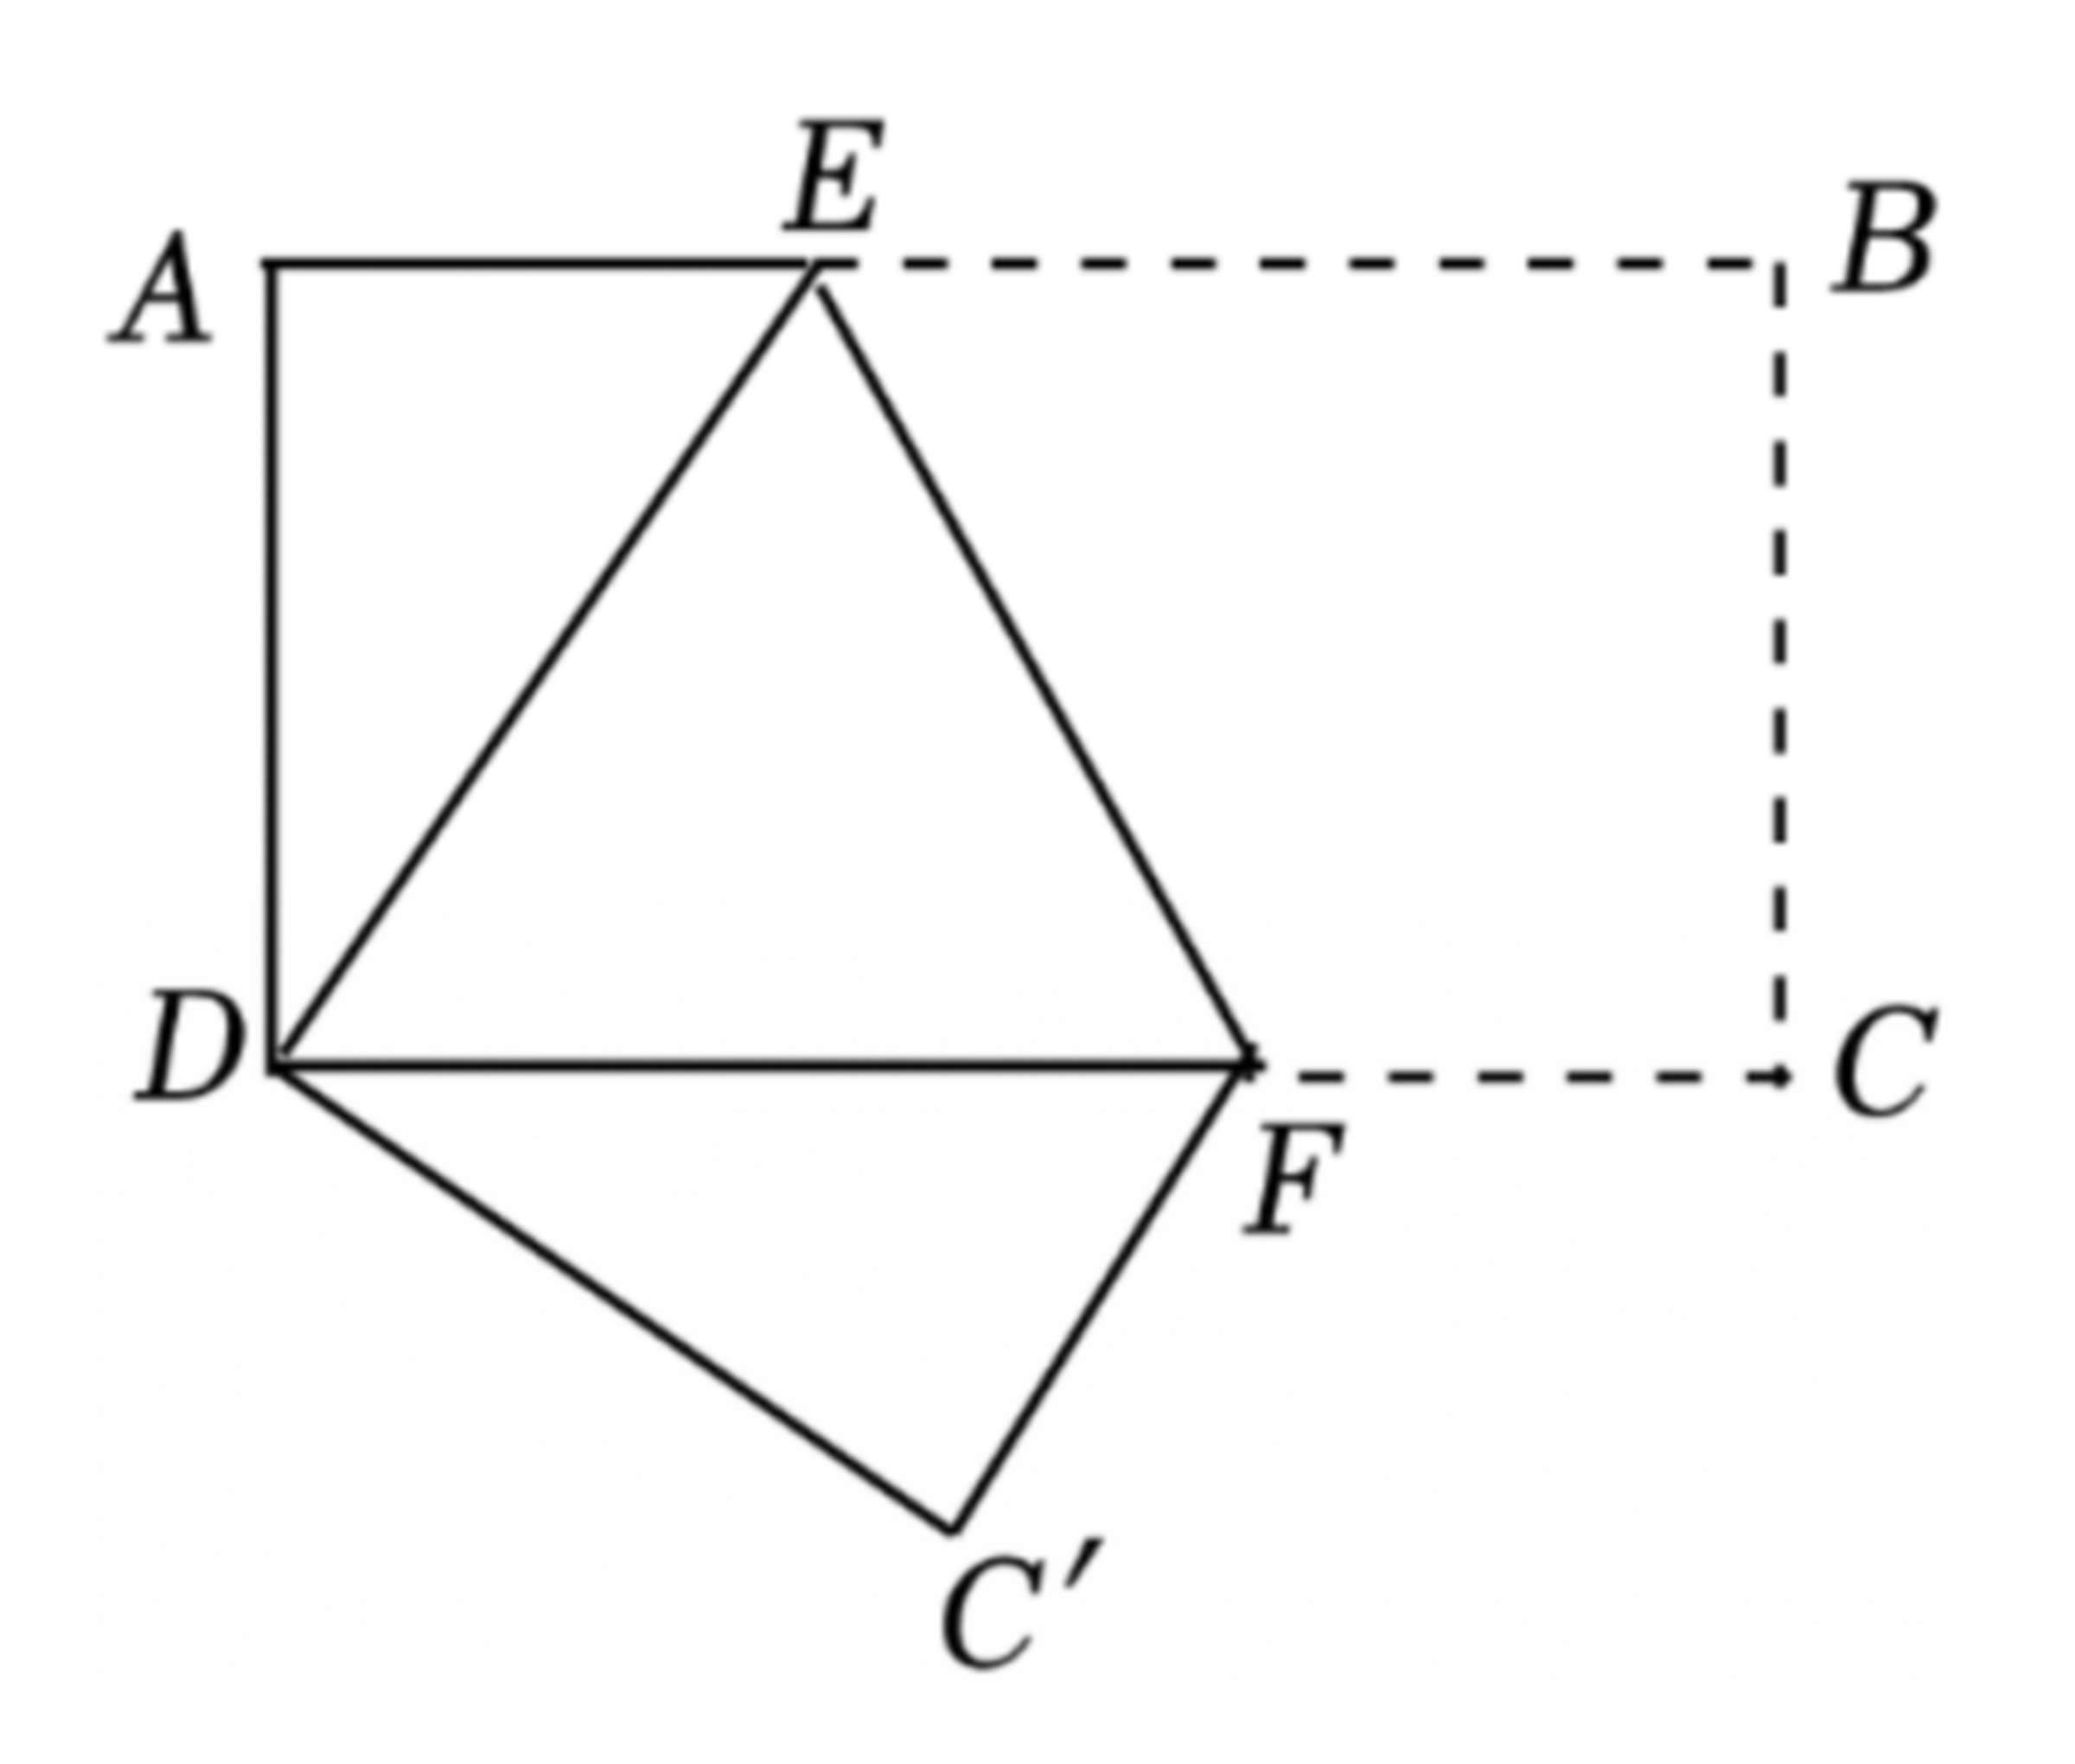
\includegraphics[width=0.40\textwidth]{figures/gao149_q11.png}
\end{center}

\ifanswer
\solbegin
\step{因为矩形 $ABCD(AB>AD)$ 的周长为 12，}
\step{在 $AB$ 和 $CD$ 边上分别取点 $E$ 和 $F$，将四边形 $BCFE$ 沿 $EF$ 折叠，}
\step{使点 $B$ 与点 $D$ 重合，此时点 $C$ 的对应点为 $C'$，}
\step{所以设 $AD=a$，$AB=b$，则 $2(a+b)=12$，}
\step{所以 $a+b=6$，且 $AB>AD$，所以 $b>a>0$，}
\step{设 $DF=x$，则 $C'F=b-x$，在 $Rt\triangle DC'F$ 中，$DC'=BC=a$，}% 几何三角形符号原卷印扁等边细线三角 $\triangle$，照录（放大 02 页确认）；$Rt$ 照录
\step{所以 $a^2+(b-x)^2=x^2$，解得 $x=\dfrac{a^2+b^2}{2b}$，}
\step{因此 $\triangle C'DF$ 的面积 $S=\dfrac{1}{2}\cdot DC'\cdot C'F=\dfrac{1}{2}\cdot a\cdot(b-x)$，}
\step{又 $b-x=b-\dfrac{(6-b)^2+b^2}{2b}=\dfrac{6(b-3)}{b}$，}
\step{所以 $S=\dfrac{1}{2}\cdot a\cdot\dfrac{6(b-3)}{b}=\dfrac{1}{2}\cdot(6-b)\cdot\dfrac{6(b-3)}{b}=\dfrac{3(6-b)(b-3)}{b}$}
\step{$=3\cdot\left(-b-\dfrac{18}{b}+9\right)$，又 $b+\dfrac{18}{b}\geqslant2\sqrt{b\cdot\dfrac{18}{b}}=6\sqrt{2}$，}
\step{当且仅当 $b=\dfrac{18}{b}$ 即 $b=3\sqrt{2}$ 时取等号，此时满足 $b>a$，}
\step{所以 $S\leqslant3\cdot(-6\sqrt{2}+9)=27-18\sqrt{2}$，故 $\triangle C'DF$ 面积的最大值为 $27-18\sqrt{2}$.}
\solend
\fi

% === Q12 === 解析内 3 幅三次函数曲线坐标图（仅答案版出）；解析 15 行（8 行 03 页＋7 行 04 页）
\item 已知 $m>0$，若存在 $t\in\R$，使得对任意 $x\in[0,m]$，不等式 $[(x-1)^2-t](x-t)\leqslant0$ 恒成立，则 $m$ 的最大值是\blankline[4.4em].

\ifanswer
\solbegin
\step{当 $t\leqslant0$ 时，$(x-1)^2-t\geqslant0$ 恒成立，}
\step{不等式 $[(x-1)^2-t](x-t)\leqslant0$ 的解集为 $x\leqslant t$，与 $x\in[0,m]$ 矛盾；}
\step{当 $t>0$ 时，不等式 $[(x-1)^2-t](x-t)\leqslant0\Leftrightarrow(x-1-\sqrt t)(x-1+\sqrt t)(x-t)\leqslant0$，}
\step{若 $t<1-\sqrt t$，即 $t\in\left(0,\dfrac{3-\sqrt5}{2}\right)$，}
\begin{center}
% 情形一 $t<1-\sqrt t$ 曲线图取 03 页右侧，去粉色水印、去色、4× LANCZOS 放大；仅答案版出
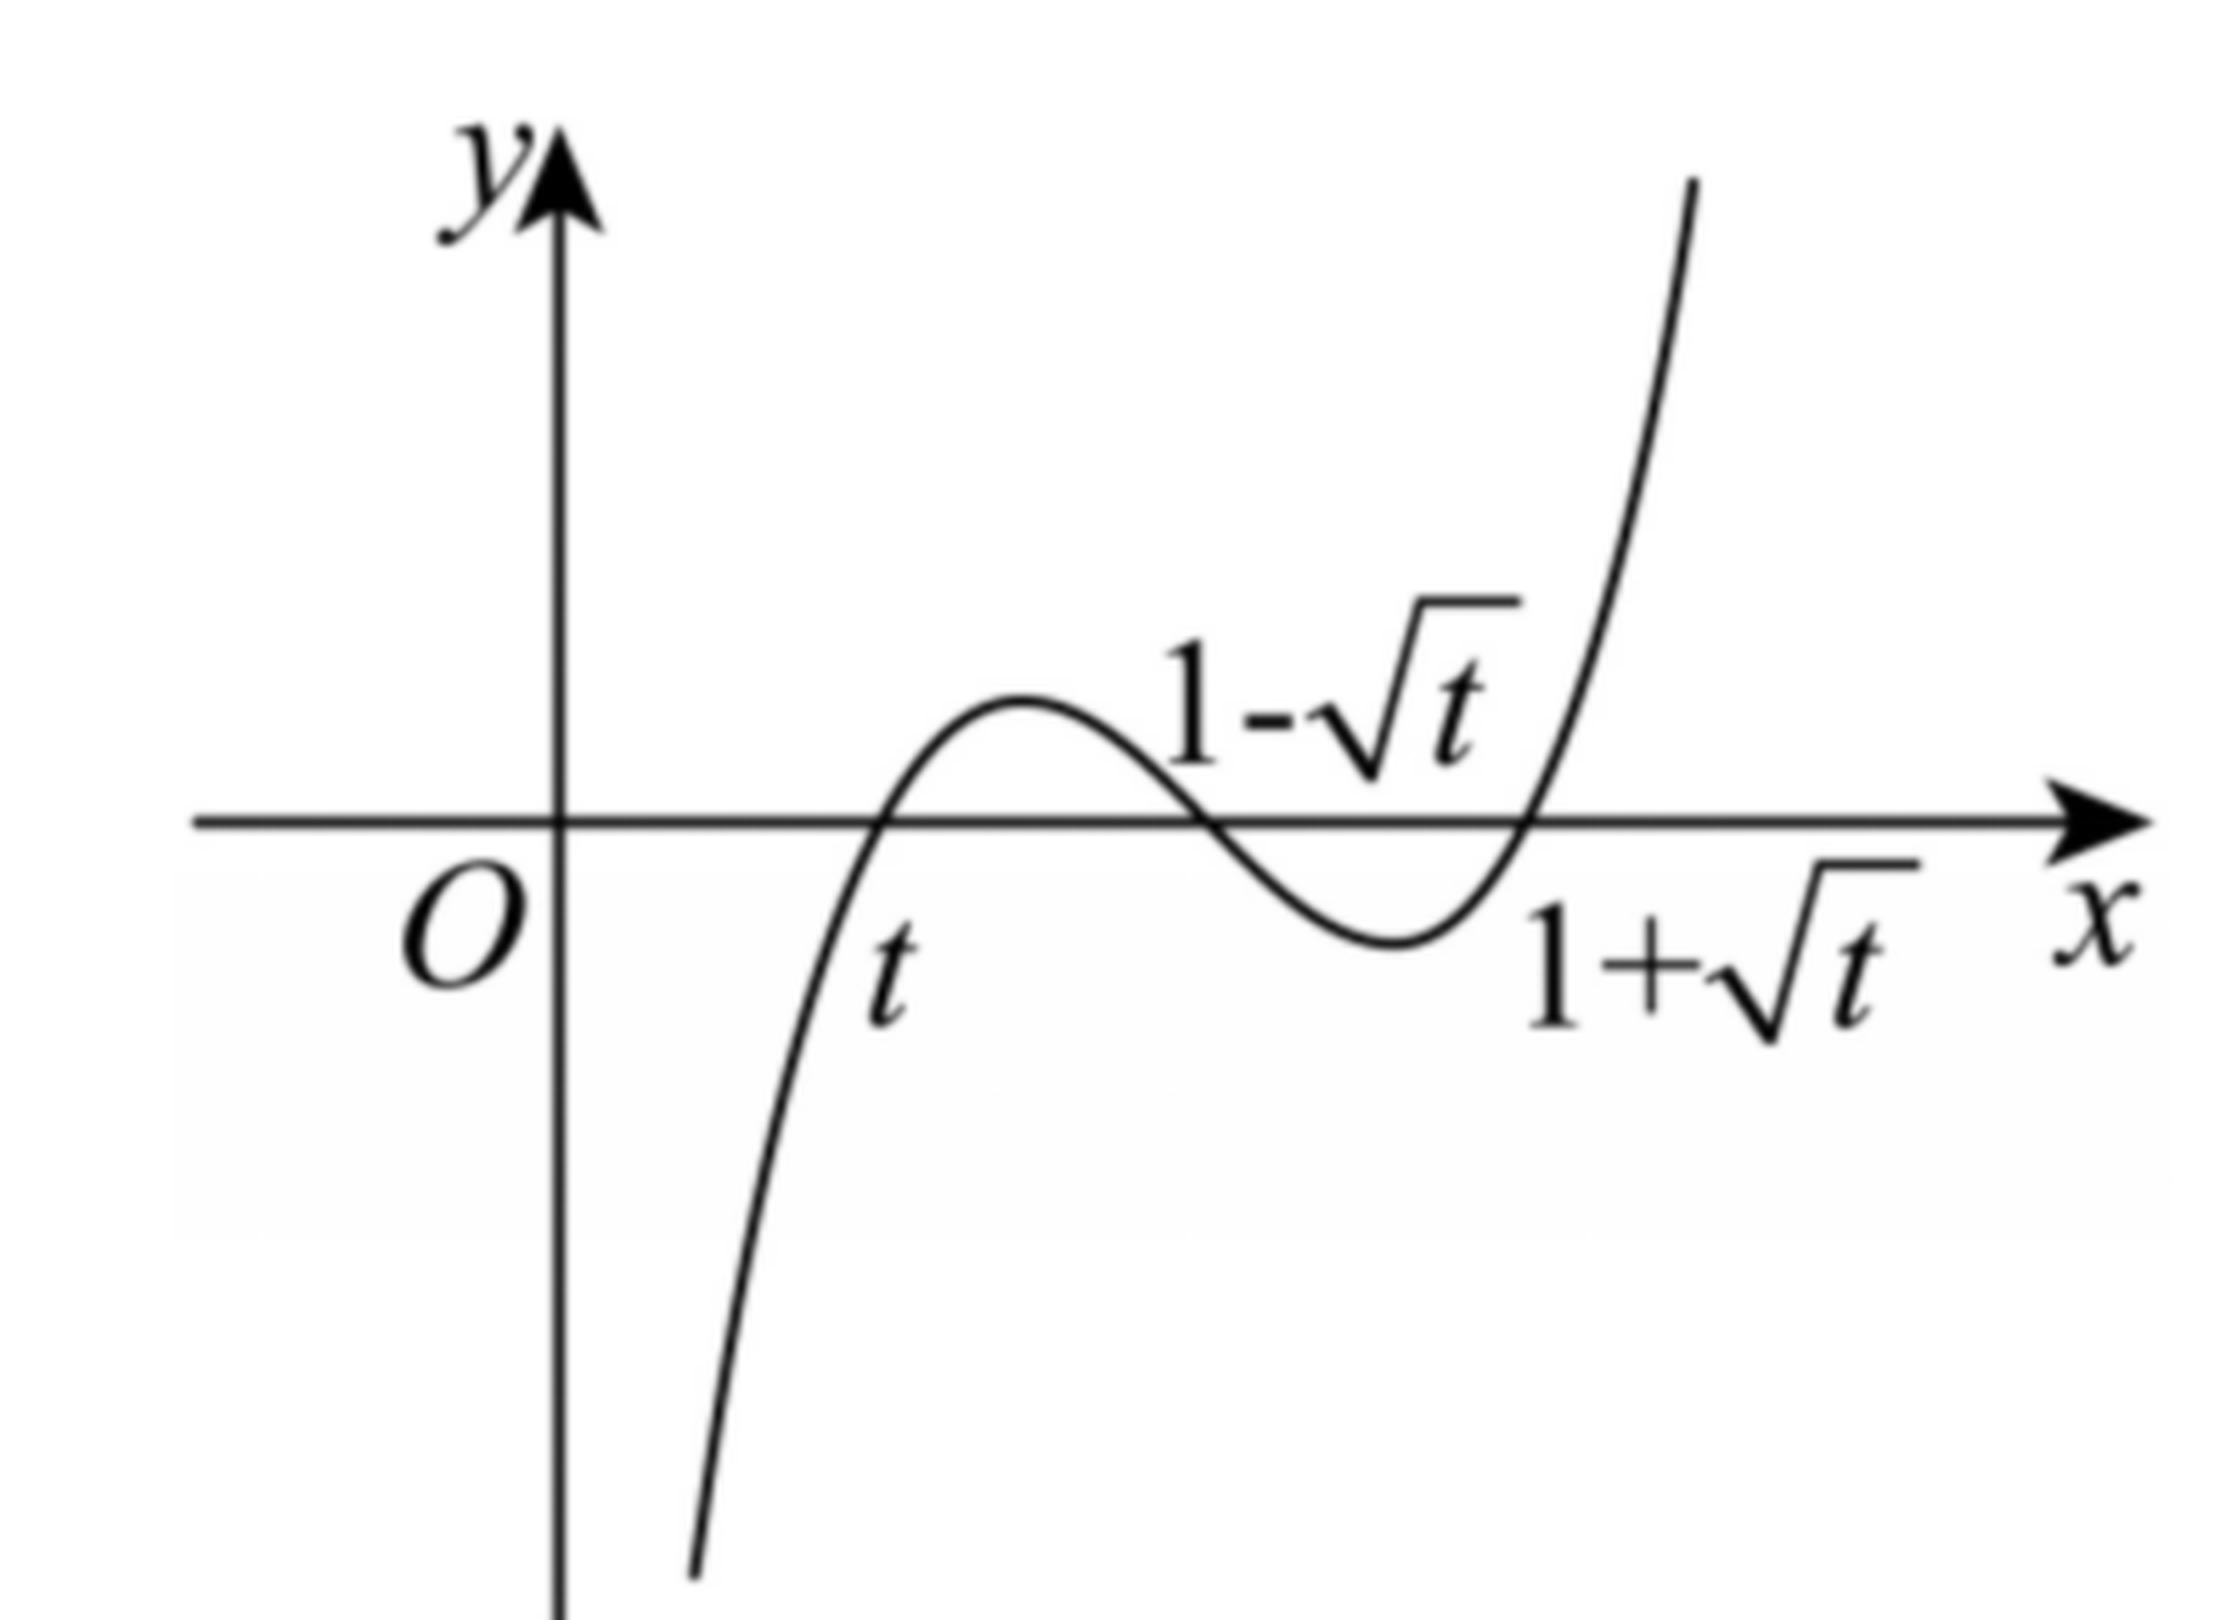
\includegraphics[width=0.40\textwidth]{figures/gao149_q12_a.png}
\end{center}
\step{则原不等式的解集为 $(-\infty,t]\cup[1-\sqrt t,1+\sqrt t]$，}
\step{当 $0<m\leqslant t$ 时，原不等式恒成立，因此}
\step{$m\in\left(0,\dfrac{3-\sqrt5}{2}\right)$；}
\step{若 $t=1-\sqrt t$，即 $t=\dfrac{3-\sqrt5}{2}$，则原不等式的解集为 $(-\infty,1+\sqrt t]$，}
\begin{center}
% 情形二 $t=1-\sqrt t$ 曲线图取 03 页右侧，去粉色水印、去色、4× LANCZOS 放大；仅答案版出
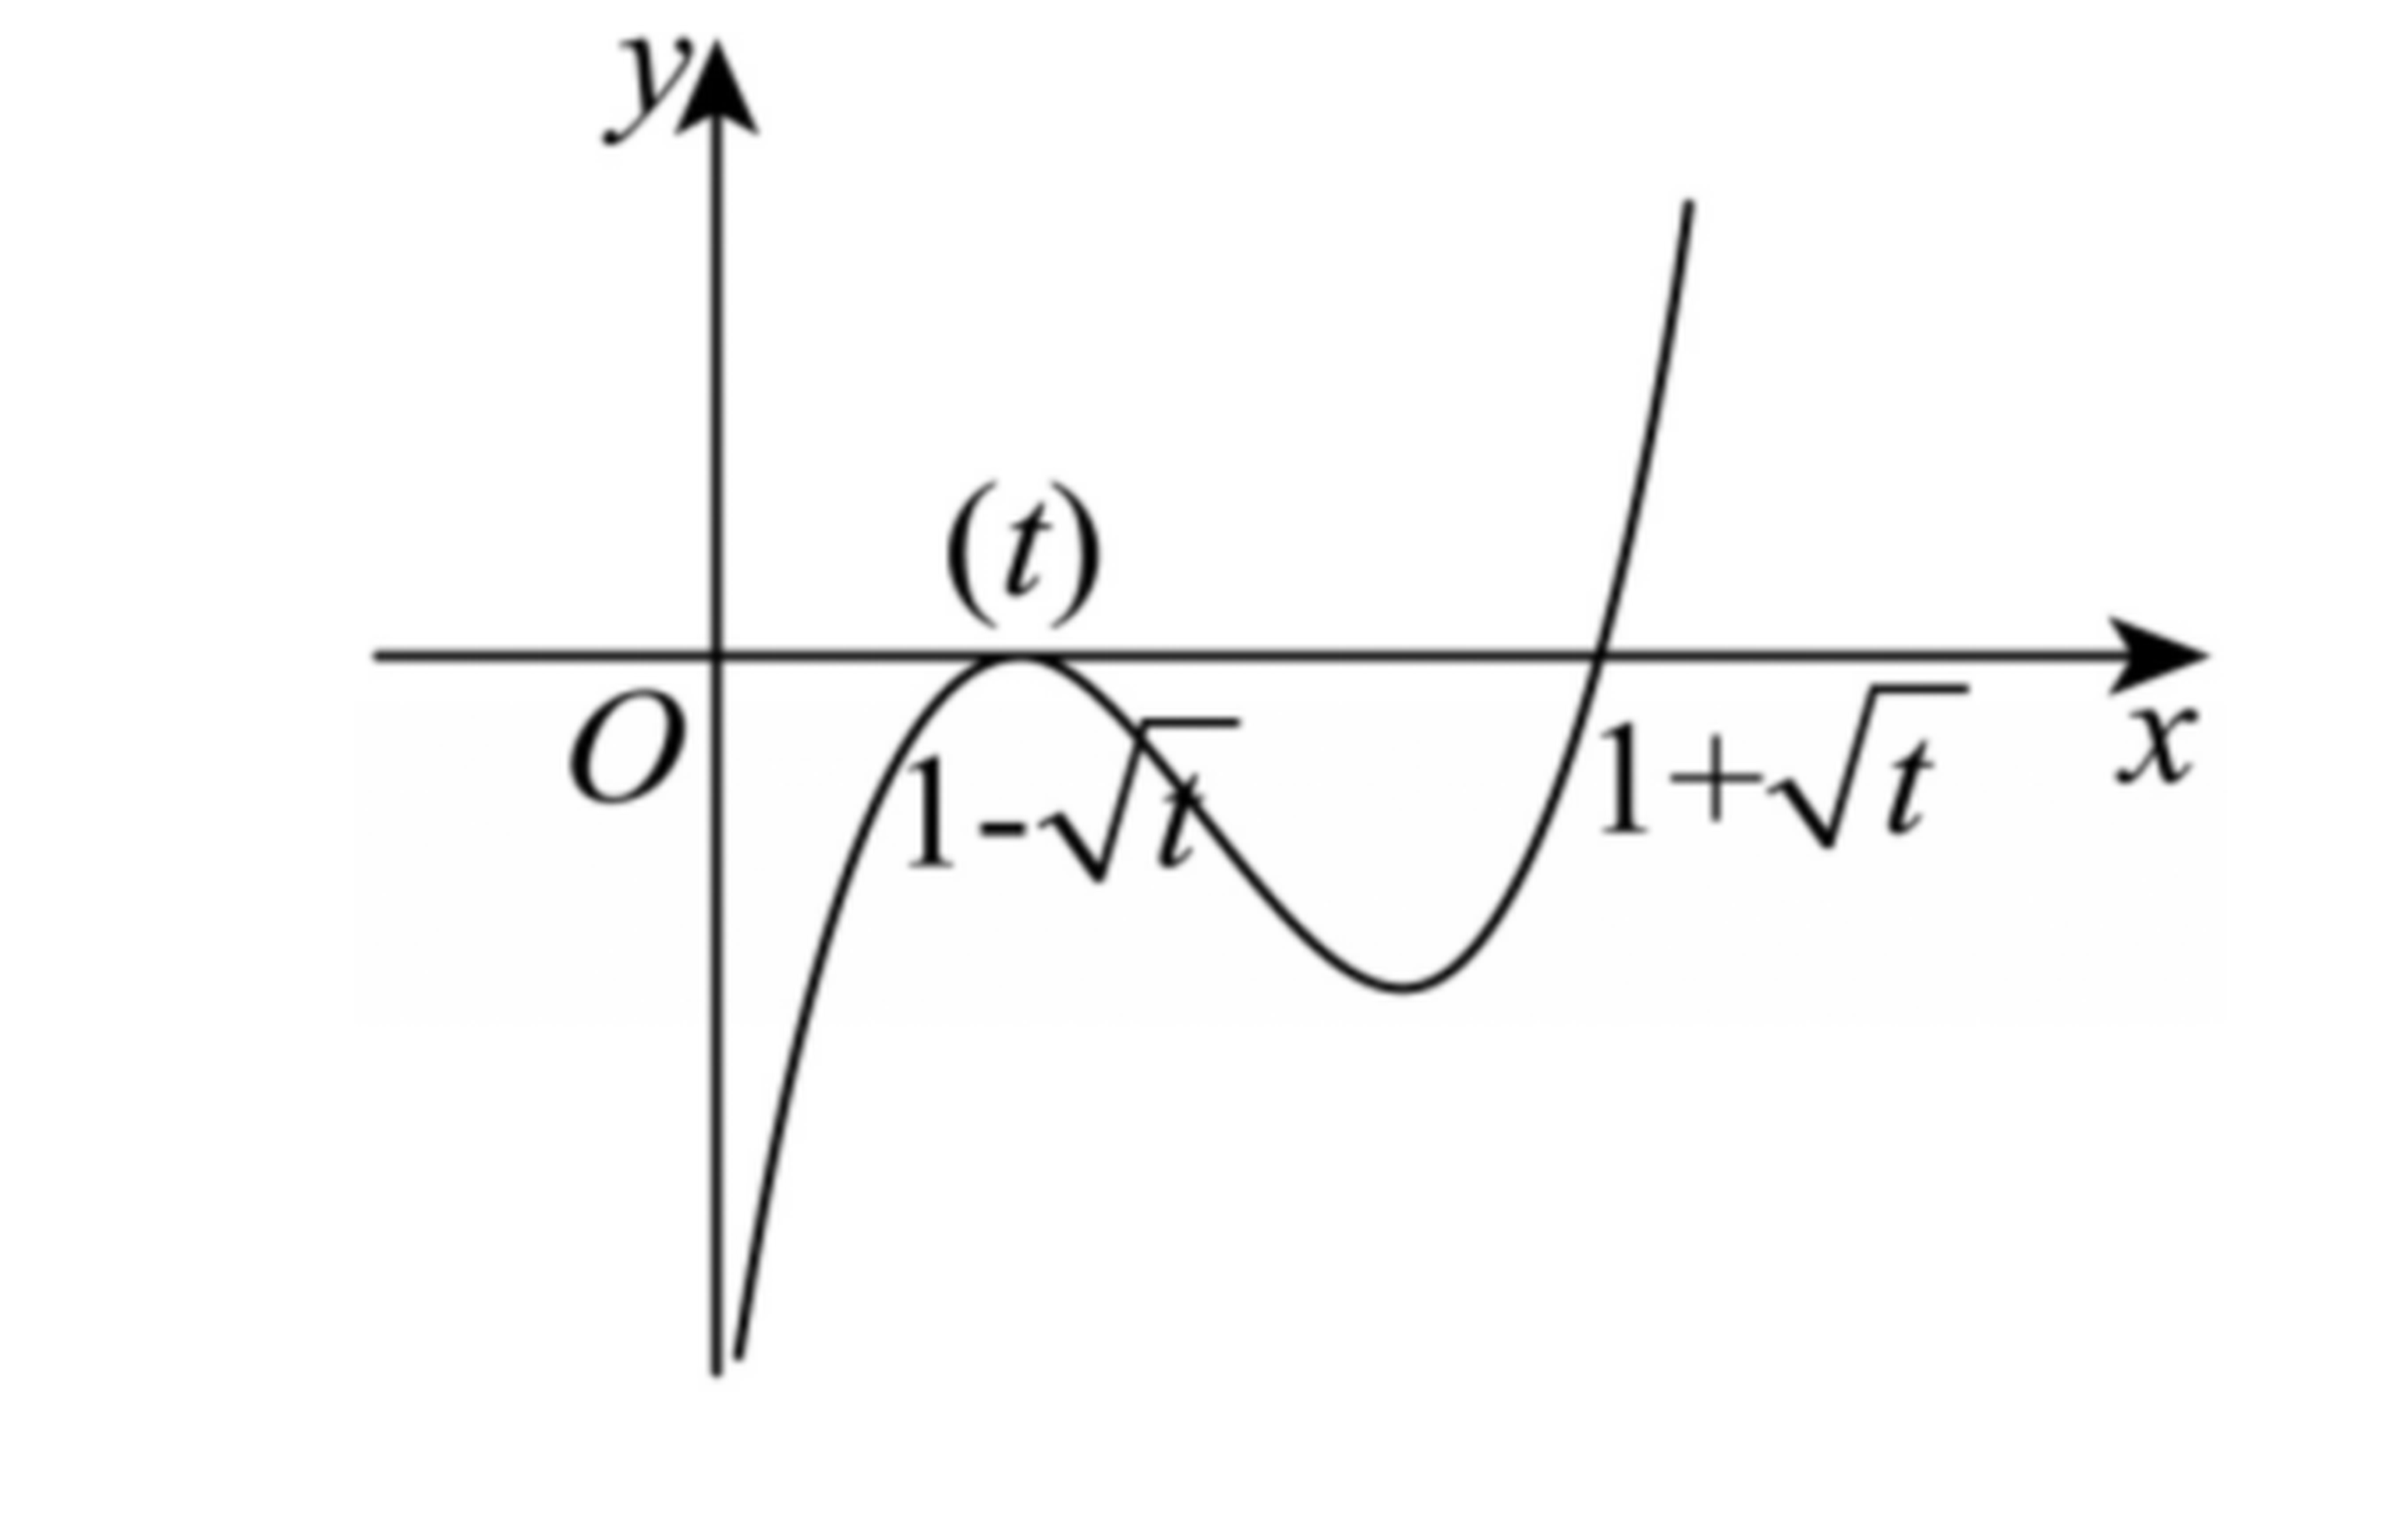
\includegraphics[width=0.40\textwidth]{figures/gao149_q12_b.png}
\end{center}
\step{当 $0<m\leqslant1+\sqrt t$ 时，原不等式恒成立，因此 $m\in\left(0,\dfrac{\sqrt5+1}{2}\right]$；}
\step{若 $1+\sqrt t>t>1-\sqrt t$，即 $t\in\left(\dfrac{3-\sqrt5}{2},\dfrac{3+\sqrt5}{2}\right)$，}
\begin{center}
% 情形三 $1+\sqrt t>t>1-\sqrt t$ 曲线图取 04 页右侧，去粉色水印、去色、4× LANCZOS 放大；仅答案版出
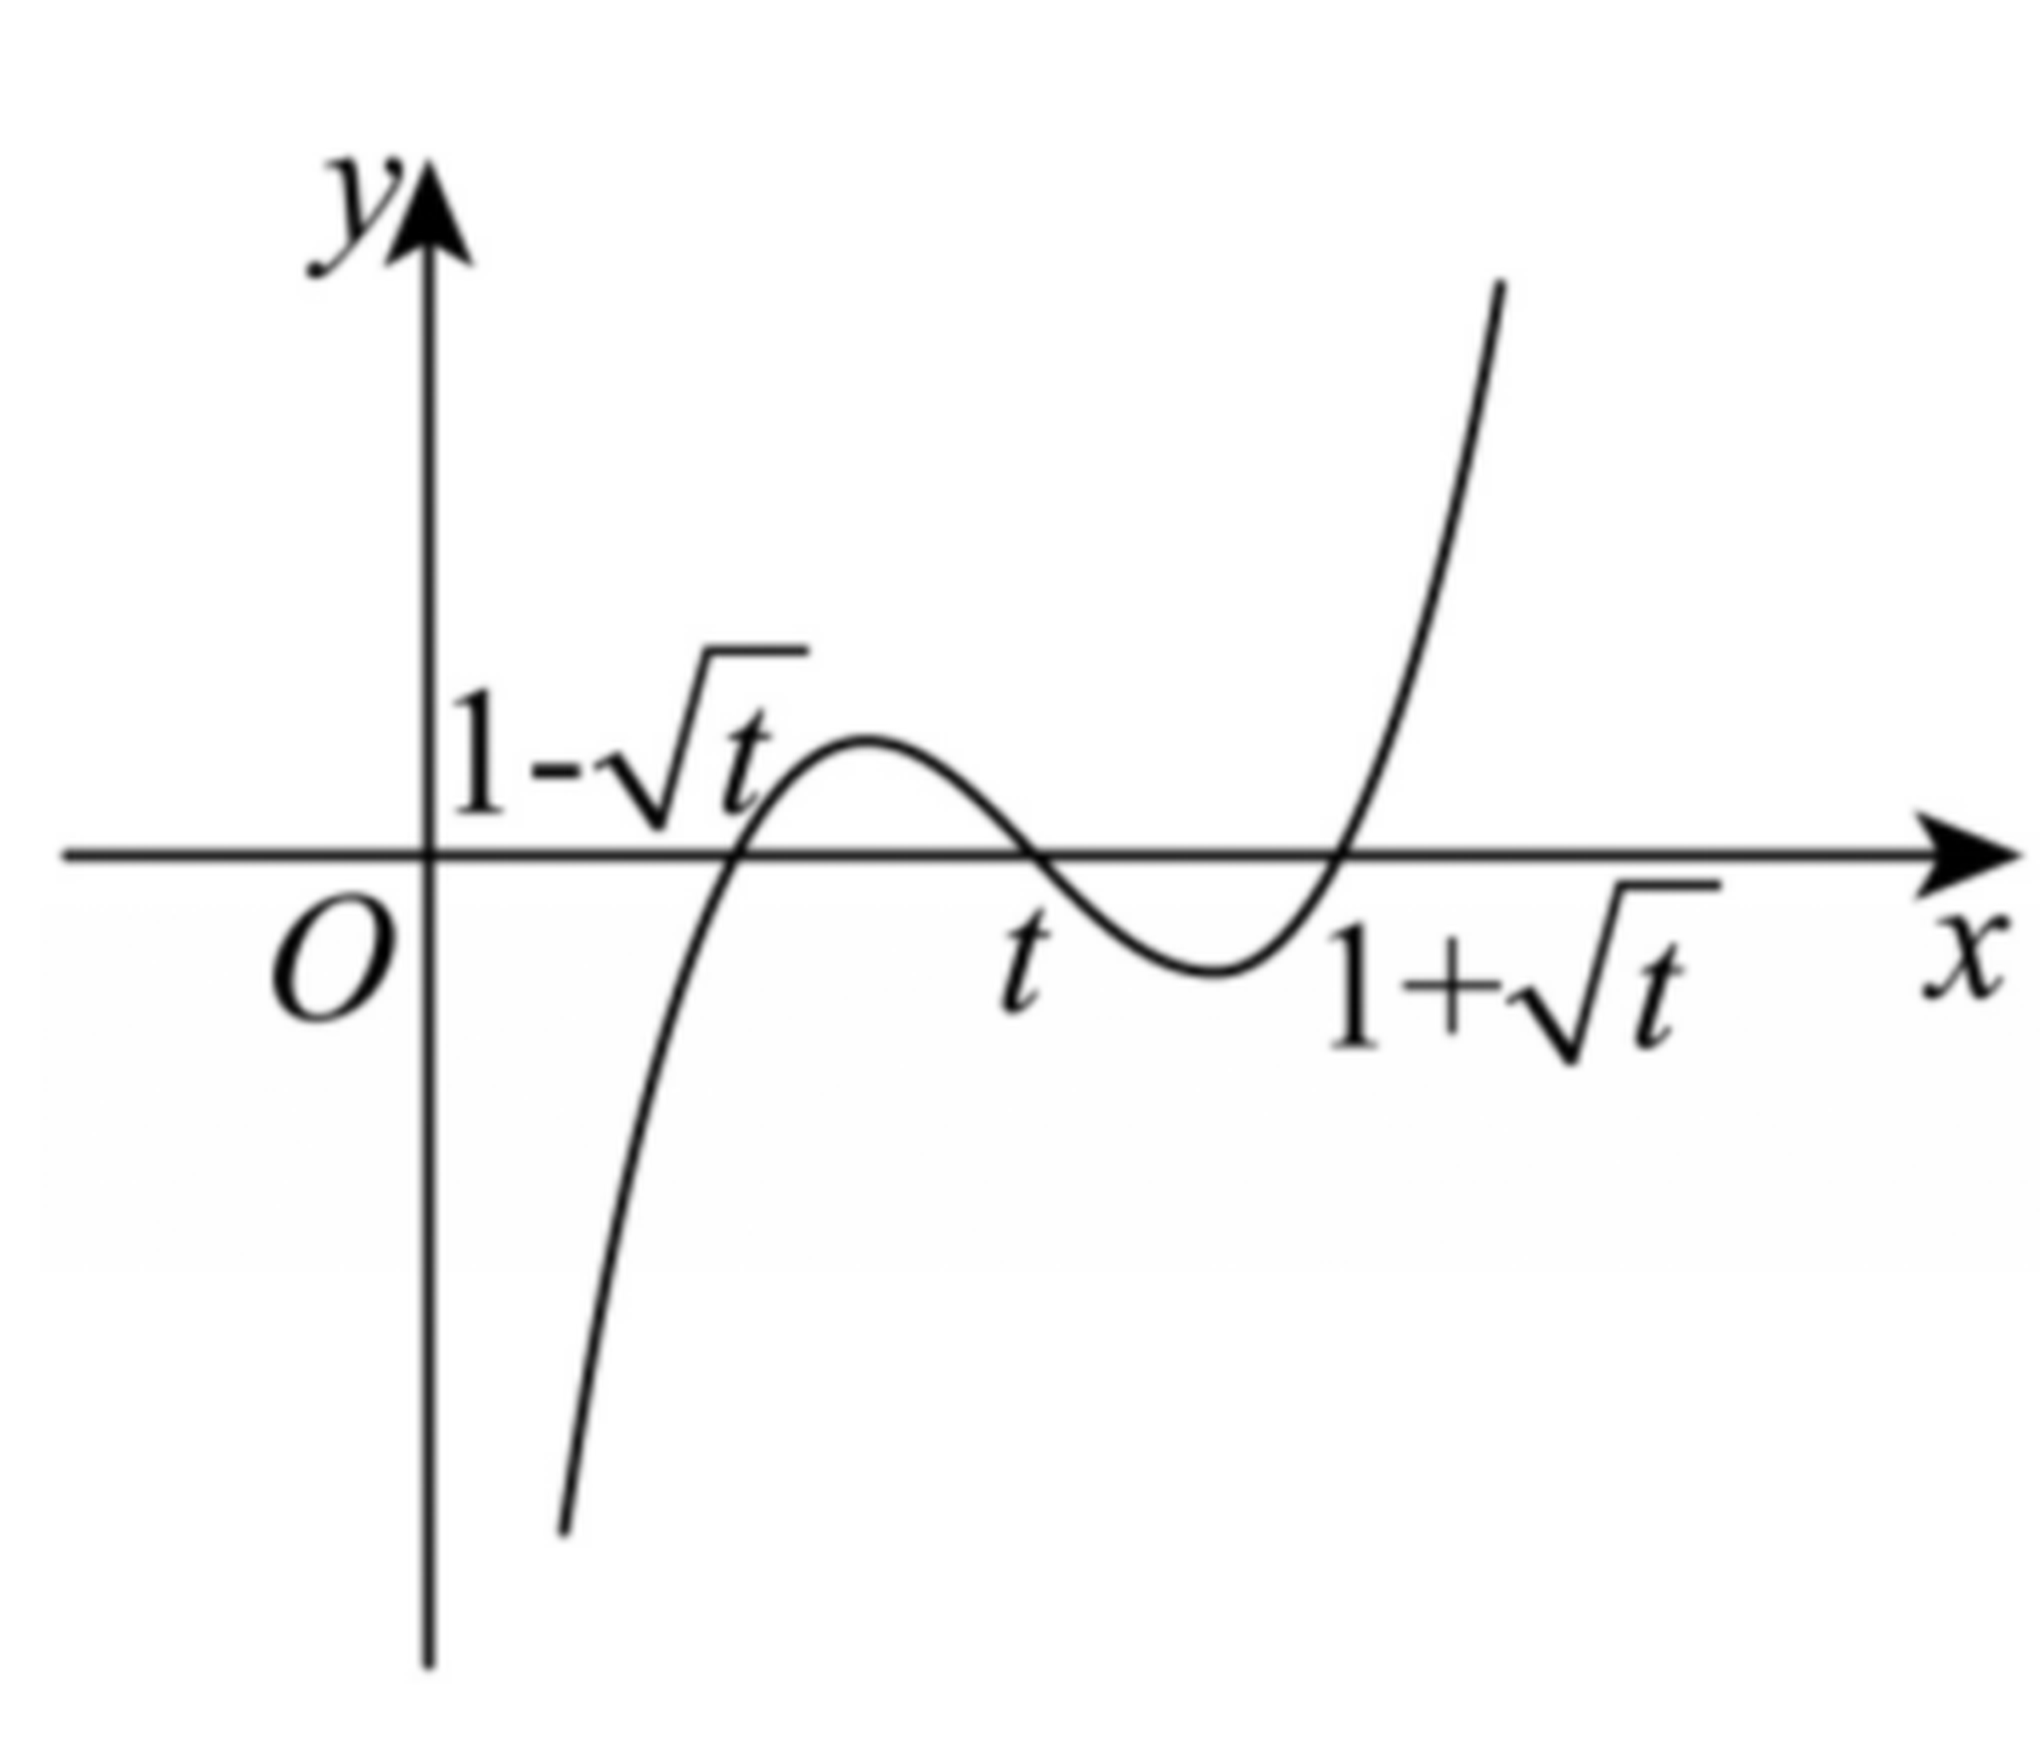
\includegraphics[width=0.40\textwidth]{figures/gao149_q12_c.png}
\end{center}
\step{则原不等式的解集为 $(-\infty,1-\sqrt t]\cup[t,1+\sqrt t]$，}
\step{当 $\begin{cases}1-\sqrt t>0\\1-\sqrt t\geqslant m\end{cases}$ 时，原不等式恒成立，此时 $t\in\left(\dfrac{3-\sqrt5}{2},1\right)$，$m\in\left(0,\dfrac{3-\sqrt5}{2}\right)$；}
\step{若 $t\geqslant1+\sqrt t$，即 $t\geqslant\dfrac{3+\sqrt5}{2}$，则取 $x=0$，$(t-1)t>0$，}
\step{原不等式不恒成立，不符合题意，}
\step{因此实数 $m$ 的取值范围是 $\left(0,\dfrac{\sqrt5+1}{2}\right]$，$m$ 的最大值是 $\dfrac{\sqrt5+1}{2}$.}
\solend
\fi

\end{enumerate}

\bigsec{二、选择题}

\begin{enumerate}
\setcounter{enumi}{12}

% === Q13 ===：答案"C"直接印在题干括号内、无【答案】/【解析】段，按 高一84 Q13／高一148 Q13 成例括号留空、另提 \ans{$C$}；四选项两行两列照原卷分行
\item 设 $ab>0$，则 $a>b$ 是 $\dfrac{1}{a}<\dfrac{1}{b}$ 的\mbox{（\quad）}

\keepwithprev
A. 充分不必要条件\qquad\qquad B. 必要不充分条件

C. 充要条件\qquad\qquad D. 既不充分又不必要条件

\ifanswer
\ans{$C$}
\fi

% === Q14 ===：$A\subset B$ 单线照录；四选项补集照原卷上划线 \overline{A}／\overline{B}；解析 1 行（由韦恩图得 B 对）
\item 已知集合 $A$、$B$ 非空，且 $A\subset B$，则下列式子中一定是空集的为\mbox{（\quad）}

\keepwithprev
A. $\overline{A}\cap B$\qquad B. $A\cap\overline{B}$\qquad C. $\overline{A}\cap\overline{B}$\qquad D. $\overline{A}\cup\overline{B}$

\ifanswer
\solbegin
\step{由韦恩图得 $B$ 对. 故选 $B$.}
\solend
\fi

% === Q15 ===："天文数字"弯引号照录；解析 2 行（首行在 04 页末、末行续 05 页顶）
\item 历史上数学计算方面的三大发明是阿拉伯数字、十进制和对数，其中对数的发明，大大缩短了计算时间，为人类研究科学和了解自然起了重大作用，对数运算对估算“天文数字”具有独特的优势. $2.5^{1000}$ 的估算值约为\mbox{（\quad）}

\keepwithprev
A. $10^{365}$\qquad B. $10^{379}$\qquad C. $10^{389}$\qquad D. $10^{398}$

\ifanswer
\solbegin
\step{$\lg 2.5^{1000}=1000\lg 2.5=1000(1-2\lg 2)\approx1000\times(1-0.602)=398$，}
\step{所以 $2.5^{1000}\approx10^{398}$. 故选 $D$.}
\solend
\fi

% === Q16 ===："完美集"新定义、圈数字①②文本模式；题干"若对任意 $x$，$y\in A$"用全角逗号、解析用顿号"$x$、$y\in A$"，两处照录不统一；解析 9 行
\item 设全集 $U=\R$，集合 $A$ 是一个非空数集，若对任意 $x$，$y\in A$，都有 $x+y\in A$、$xy\in A$，则称集合 $A$ 为一个“完美集”，给出以下命题：

①若 $A_1$、$A_2$ 都是“完美集”，且 $A_1\cap A_2\ne\varnothing$，则 $A_1\cap A_2$ 也是“完美集”；

②若 $A_1$、$A_2$ 都是“完美集”，则 $A_1\cup A_2$ 也是“完美集”.

下列说法正确的是\mbox{（\quad）}

\keepwithprev
A. ①②都是真命题\qquad\qquad B. ①是真命题，②是假命题

C. ①是假命题，②是真命题\qquad\qquad D. ①②都是假命题

\ifanswer
\solbegin
\step{由题意，全集 $U=\R$，集合 $A$ 是一个非空数集，}
\step{若对任意 $x$、$y\in A$，都有 $x+y\in A$、$xy\in A$，则称集合 $A$ 为一个“完美集”，}
\step{对于①，取 $x$、$y\in A_1\cap A_2$，则 $x\in A_1$，$x\in A_2$，$y\in A_1$，$y\in A_2$，}
\step{又 $A_1$、$A_2$ 是“完美集”，所以 $x+y\in A_1$，$xy\in A_1$，$x+y\in A_2$，$xy\in A_2$，}
\step{所以 $x+y\in A_1\cap A_2$，$xy\in A_1\cap A_2$，所以 $A_1\cap A_2$ 是“完美集”，故①正确；}
\step{对于②，取“完美集” $A_1=\{x\mid x=2k,k\in\Z\}$，$A_2=\{x\mid x=3k,k\in\Z\}$，}
\step{则 $2\in A_1$，$3\in A_2$，但 $2+3\notin A_1\cup A_2$，}
\step{即此时 $A_1\cup A_2$ 不是“完美集”，故②错误.}
\step{故选 $B$.}
\solend
\fi
\end{enumerate}

\bigsec{三、解答题}

\begin{enumerate}
\setcounter{enumi}{16}

% === Q17 ===："图像"（有亻）照录（Q17 题干与解析共 2 处）；绝对值 \lvert…\rvert；解析 7 行
\item 已知 $m\in\R$，$f(x)=(m^2-m-5)x^m$. 若 $y=f(x)$ 是幂函数，且其图像不经过原点.

(1) 求实数 $m$ 的值；

(2) 若 $f(a)=f(b)$ 且 $a\ne b$，求 $\lvert a+2\rvert+\lvert b-1\rvert$ 的最小值，并指出取到最小值时 $a$ 的取值范围.

\ifanswer
\solbegin
\step{(1) $f(x)=(m^2-m-5)x^m$ 是幂函数，得 $m^2-m-5=1$，即 $m^2-m-6=0$，}
\step{解得 $m=-2$ 或 $m=3$，又函数图像不经过原点，所以 $m=-2$($3$ 舍)；}
\step{(2) 由 (1) 得 $f(x)=x^{-2}=\dfrac{1}{x^2}$ 为偶函数，}
\step{$x<0$ 时，函数 $f(x)$ 严格增，$x>0$ 时，函数 $f(x)$ 严格减，}
\step{又 $f(a)=f(b)$ 且 $a\ne b$，所以 $a=-b$，且 $a\ne0$，$b\ne0$，}
\step{则 $\lvert a+2\rvert+\lvert b-1\rvert=\lvert a+2\rvert+\lvert-a-1\rvert=\lvert a+2\rvert+\lvert a+1\rvert$，}
\step{则 $\lvert a+2\rvert+\lvert b-1\rvert$ 的最小值为 $1$，取到最小值时 $a$ 的取值范围是 $[-2,-1]$.}
\solend
\fi

% === Q18 ===：判别式两形混用——(1) cases 块印高 \Delta、(2) 独立行印扁 \triangle，逐处照录不统一；解析 8 行
\item 已知命题 $p$：方程 $x^2+4x+m-1=0$ 有两个不等的负根；命题 $q$：方程 $4x^2+4x+m-2=0$ 无实根.

(1) 若 $p$ 为真命题，求 $m$ 的取值范围；

(2) 若 $p$、$q$ 两命题一真一假，求 $m$ 的取值范围.

\ifanswer
\solbegin
\step{(1) 若 $p$ 为真命题，即方程 $x^2+4x+m-1=0$ 有两个不等的负根；}
\step{必有 $\begin{cases}\Delta=16-4(m-1)>0\\m-1>0\end{cases}$，解得 $1<m<5$，即 $m$ 的取值范围为 $(1,5)$；}
\step{(2) 命题 $q$：方程 $4x^2+4x+m-2=0$ 无实根，}
\step{则有 $\triangle=16-16(m-2)<0$，解得 $m>3$，}
\step{若 $p$ 和 $q$ 有且只有一个为真命题，}
\step{若 $p$ 真 $q$ 假，必有 $\begin{cases}1<m<5\\m\leqslant3\end{cases}$，则有 $1<m\leqslant3$，}
\step{若 $p$ 假 $q$ 真，必有 $\begin{cases}m\leqslant1\text{ 或 }m\geqslant5\\m>3\end{cases}$，则有 $m\geqslant5$，}
\step{综上，$1<m\leqslant3$ 或 $m\geqslant5$.}
\solend
\fi

% === Q19 ===：$A\subseteq B$ 带下划线照录；解析 7 行（(2) 两组 cases 并排）
\item 已知 $m\in\R$，集合 $A=\left\{x\mid y=\sqrt{3-x}-\dfrac{1}{\sqrt{x-1}}\right\}$，集合 $B=\{x\mid 2m\leqslant x\leqslant1-m\}$.

(1) 若 $A\cup B=B$，求实数 $m$ 的取值范围；

(2) 若 $A\cap B=\varnothing$，求实数 $m$ 的取值范围.

\ifanswer
\solbegin
\step{(1) 函数 $y=\sqrt{3-x}-\dfrac{1}{\sqrt{x-1}}$，则 $\begin{cases}3-x\geqslant0\\x-1>0\end{cases}$，解得 $1<x\leqslant3$，}
\step{所以 $A=\{x\mid1<x\leqslant3\}$，}
\step{因为 $A\cup B=B$，所以 $A\subseteq B$，则 $\begin{cases}2m\leqslant1\\1-m\geqslant3\end{cases}$，解得 $m\leqslant-2$，}
\step{综上，实数 $m$ 的取值范围为 $(-\infty,-2]$；}
\step{(2) 当 $B=\varnothing$ 时，则 $2m>1-m$，解得 $m>\dfrac{1}{3}$，}
\step{当 $B\ne\varnothing$ 时，则 $\begin{cases}2m\leqslant1-m\\2m>3\end{cases}$ 或 $\begin{cases}2m\leqslant1-m\\1-m\leqslant1\end{cases}$，解得 $m\in\varnothing$ 或 $0\leqslant m\leqslant\dfrac{1}{3}$，}
\step{综上，实数 $m$ 的取值范围为 $[0,+\infty)$.}
\solend
\fi

% === Q20 ===：n 阶基本不等式推广；(3) 解析含 \overbrace{…}^{k} 上括号；(2) 解析"x=x=x=3(1-x)"三连等系原卷笔误、照录加注（见 ⑤）；解析 14 行
\item 教材中的基本不等式可以推广到 $n$ 阶：$n$ 个正数的算术平均数不小于它们的几何平均数，即对于任意的正数 $a_1$、$a_2$、$\cdots$、$a_n$，有 $\dfrac{a_1+a_2+\cdots+a_n}{n}\geqslant\sqrt[n]{a_1\cdot a_2\cdots a_n}$（$n\in\N$ 且 $n\geqslant2$），且等号当且仅当 $a_1=a_2=\cdots=a_n$ 时成立. 利用此结论解决下列问题：

(1) 若 $x$、$y$、$z>0$，求 $\dfrac{y}{x}+\dfrac{2z}{y}+\dfrac{4x}{z}$ 的最小值；

(2) 已知 $0<x<1$，求 $x^3(1-x)$ 的最大值，并求取得最大值时的 $x$ 的值；

(3) 对任意的正整数 $k$，判断 $\left(1+\dfrac{1}{k}\right)^k$ 与 $\left(1+\dfrac{1}{k+1}\right)^{k+1}$ 的大小关系，并证明.

\ifanswer
\solbegin
\step{(1) 因为 $x$、$y$、$z>0$，有 $\dfrac{y}{x}>0$，$\dfrac{2z}{y}>0$，$\dfrac{4x}{z}>0$}
\step{所以 $\dfrac{y}{x}+\dfrac{2z}{y}+\dfrac{4x}{z}\geqslant3\sqrt[3]{\dfrac{y}{x}\cdot\dfrac{2z}{y}\cdot\dfrac{4x}{z}}=3\sqrt[3]{8}=6$，}
\step{当且仅当 $\dfrac{y}{x}=\dfrac{2z}{y}=\dfrac{4x}{z}$ 时取等号，故 $\dfrac{y}{x}+\dfrac{2z}{y}+\dfrac{4x}{z}$ 的最小值为 $6$.}
\step{(2) 因为 $0<x<1$，所以 $1-x>0$，}
\step{$x^3(1-x)=\dfrac{1}{3}[x\cdot x\cdot x\cdot3(1-x)]\leqslant\dfrac{1}{3}\left[\dfrac{x+x+x+3(1-x)}{4}\right]^4=\dfrac{1}{3}\times\left(\dfrac{3}{4}\right)^4$}
\step{$=\dfrac{27}{256}$，当且仅当 $x=x=x=3(1-x)$，即 $x=3(1-x)$，$x=\dfrac{3}{4}$ 取等号，}% 原卷"x=x=x=3(1-x)"三连等，疑为四因子相等之误排，放大 08 页确认，照录未改（见 ⑤）
\step{所以 $0<x<1$ 时，$x^3(1-x)$ 的最大值是 $\dfrac{27}{256}$，取最大值时 $x=\dfrac{3}{4}$.}
\step{(3) 对任意 $k\in\N^*$，$\left(1+\dfrac{1}{k}\right)^k<\left(1+\dfrac{1}{k+1}\right)^{k+1}$.}
\step{证明：$\left(1+\dfrac{1}{k}\right)^k=\overbrace{\left(1+\dfrac{1}{k}\right)\cdot\left(1+\dfrac{1}{k}\right)\cdots\left(1+\dfrac{1}{k}\right)}^{k}\times1$}
\step{$\leqslant\left(\dfrac{\overbrace{\left(1+\dfrac{1}{k}\right)+\left(1+\dfrac{1}{k}\right)+\cdots+\left(1+\dfrac{1}{k}\right)}^{k}+1}{k+1}\right)^{k+1}$}
\step{$=\left(\dfrac{\overbrace{(1+1+\cdots+1)}^{k}+\overbrace{\left(\dfrac{1}{k}+\dfrac{1}{k}+\cdots+\dfrac{1}{k}\right)}^{k}+1}{k+1}\right)^{k+1}=\left(\dfrac{k+1+1}{k+1}\right)^{k+1}=\left(1+\dfrac{1}{k+1}\right)^{k+1}$，}
\step{当且仅当 $1+\dfrac{1}{k}=1$ 时取等号，}
\step{但是任意 $k\in\N^*$ 时 $1+\dfrac{1}{k}>1$，所以等号不成立，}
\step{故任意 $k\in\N^*$ 时，$\left(1+\dfrac{1}{k}\right)^k<\left(1+\dfrac{1}{k+1}\right)^{k+1}$.}
\solend
\fi

% === Q21 ===："减 k 集"新定义（引号内 k／数字两侧空格照录）；解析 26 行（续 10 页），含 ⑤ 三处原卷笔误照录
\item 定义：对于给定的整数 $k$，若非空集合 $A$ 满足如下 3 个条件：

① $A$ 是正整数集的子集；② $A\ne\{1\}$；

③对任意正整数 $x,y$，若 $x+y\in A$，则 $xy-k\in A$；则称集合 $A$ 为“减 $k$ 集”.

(1) 判断集合 $A=\{1,2\}$ 是否为“减 $0$ 集”？是否为“减 $1$ 集”？（无需说明理由）

(2) 证明：不存在“减 $2$ 集”；

(3) 是否存在“减 $1$ 集”？如果存在，求出所有“减 $1$ 集”；如果不存在，说明理由.

\ifanswer
\solbegin
\step{(1) 因为 $P\subseteq\N^*$，$P\ne\{1\}$，$1+1=2\in P$，$1\times1-0\in P$，}
\step{所以集合 $P=\{1,2\}$ 是“减 $0$ 集”；}
\step{因为 $P\subseteq\N^*$，$P\ne\{1\}$，$1+1=2\in P$，$1\times1-1\notin P$，}
\step{所以集合 $P=\{1,2\}$ 是“减 $1$ 集”；}% 按条件③应为"不是"，原卷径印"是"，放大 09 页确认，照录未改（见 ⑤）
\step{(2) 假设存在集合 $A$ 是“减 $2$ 集”，若 $x+y\in A$，则 $xy-2\in A$，}
\step{①当 $x+y=xy-2$ 时，有 $(x-1)(y-1)=3$，}
\step{则 $x$、$y$ 一个为 $2$，一个为 $4$，所以集合 $A$ 有元素 $6$，}
\step{但 $3+3\in A$，$3\times3-2\notin A$，与 $A$ 是“减 $2$ 集”矛盾；}
\step{②当 $x+y\ne xy-2$ 时，则 $x+y=xy-1$ 或 $x+y=xy-m$($m>2$)，}
\step{若 $x+y=xy-1$，$m=1$ 时，$M$ 为除 $1$ 以外的最小元素，}% 原卷"m=1"上文未显式定义，疑笔误，放大 09 页确认，照录未改（见 ⑤）
\step{则 $x=M-1$，$y=1$ 时，$xy-2=M-3$ 小于 $M$，}
\step{要符合题意，必须 $M=4$，}
\step{此时取 $x-2$，$y=2$，$xy-2=2$ 不属于 $A$，故不符合题意，}% 原卷"取 x−2"疑为"取 x=2"误排，放大 09 页确认，照录未改（见 ⑤）
\step{当 $m>2$ 时，$(x-1)(y-1)=m+1$，同样得出矛盾，}
\step{综上，不存在 $A$ 是“减 $2$ 集”.}
\step{(3) 存在“减 $1$ 集” $A$，则 $A\ne\{1\}$，}
\step{①假设 $1\in A$，则 $A$ 中除了元素 $1$ 以外，必然还含有其它元素，}
\step{假设 $2\in A$，$1+1\in A$，而 $1\times1-1\notin A$，所以 $2\notin A$，}
\step{假设 $3\in A$，$1+2\in A$，而 $1\times2-1\in A$，所以 $3\in A$，}
\step{所以 $A=\{1,3\}$，}
\step{假设 $4\in A$，$1+3\in A$，而 $1\times3-1\notin A$，所以 $4\notin A$，}
\step{假设 $5\in A$，$1+4\in A$，$1\times4-1\in A$，$2+3=5$，$2\times3-1\in A$，所以 $5\in A$，}
\step{所以 $A=\{1,3,5\}$，}
\step{以此类推，得 $A=\{1,3,5,\cdots,2n-1,\cdots\}$，($n\in\N^*$)，}
\step{所以所有的“减 $1$ 集”有 $\{1,3\}$，$\{1,3,5\}$，$\{1,3,5,7\}$，$\cdots$，$\{1,3,5,\cdots,2n-1,\cdots\}$，}
\step{$(n\in\N^*)$.}
\solend
\fi
\end{enumerate}

\end{document}
"
%
% ① 原始材料：微信公众号"魔都数学加油站"文章，连载"27学年高一149"，原文标题
% "27学年高一149——2026-2027年上海市青浦高级中学上外云间高一上期中"；
% 原文链接：https://mp.weixin.qq.com/s/T7_nyoR1k0o_5og7FkDsyw 。
% 正文为 10 张 PNG 页（01/02/03/04/10 为 2560×3620，05/06/07/08/09 为 4762×6735，
% 同一篇各页分辨率混排，逐页按各自分辨率裁图核对，别按预览比例换算裁框）。
% 体例：混合体例讲评版——19 题中 Q6 只印【答案】、无【解析】；Q13 的答案"C"
%   直接印在题干括号内、无【答案】/【解析】段；其余 17 题印【解析】（逐题核实，见 ② ②）。
% 题目、答案、解析均据原图转录；卷面粉红色水印"魔都数学加油站"及公众号页脚未录入。
% 全卷插图清单（逐页通读 10 页确认）：1 幅题目配图 + 3 幅【解析】内配图：
%   · Q11 矩形 ABCD 折叠几何图（02 页右侧：A/B/C/D/E/F/C' 与虚线 EB、BC、FC），
%     题干"如图"处，题目配图、三版都出，裁 figures/gao149_q11.png；
%   · Q12【解析】内 3 幅三次函数曲线坐标图（03 页右侧两幅 + 04 页右侧一幅：
%     x/y 轴、O、t、1-\sqrt t、1+\sqrt t 等标注，分别对应 t<1-\sqrt t、
%     t=1-\sqrt t、1+\sqrt t>t>1-\sqrt t 三种情形），解析配图、仅答案版出，
%     分别裁 figures/gao149_q12_a.png／_b.png／_c.png，放 \ifanswer 内 \step 之间
%     （高一73 第 16 题成例）；
%   其余各页逐页确认无其它题目配图、无表格；Q14 解析"由韦恩图得 B 对"仅文字推导、
%   原卷并未印韦恩图；Q9／Q18／Q19 的 cases 块与 Q20(3) 的 \overbrace 为数学块（非图）；
%   10 页下半仅水印、无正文。4 图均取自原卷截图，去粉色水印、去色、4× LANCZOS 放大。
%
% 卷首标题：原卷印作"2026-2027 年青浦高级中学上外云间高一上期中"，年份区间按全稿
% 惯例排 en dash；原卷卷面未印副标题，本稿按同期中卷（高一140／141／143／144／145／
% 146／147／148）知识模块口径补出"集合与常用逻辑用语、不等式、函数"。
%
% 题号体例（逐页核实定稿）：本卷共 19 题——一、填空题 3—12（10 题）、
% 二、选择题 13—16（4 题）、三、解答题 17—21（5 题）。
% 三节分别 \setcounter{enumi}{2}／{12}／{16}。原卷从第 3 题起、无第 1、2 题，
% 本稿保留原题号；全卷无附加题节（Q21 解析末行"（n\in N^*）."为全卷收尾）。
%
% ② 与原卷的排版差异：
%   ① 原文从第 3 题起，本稿保留原题号；共 19 题三节；
%   ② 混合体例逐题核实：Q6（反证法"假设的内容"）只印【答案】、无【解析】，
%      按 高一140 第 5 题／高一145 Q3 成例提 \ans{}、不补造解析；Q13 答案"C"直接
%      印在题干括号内、全卷无该题【答案】/【解析】段，按 高一84 Q13／高一148 Q13
%      成例括号 \mbox{（\quad）} 留空、另提 \ans{$C$}；其余 17 题印【解析】、
%      用 \solbegin…\solend，选择题答案在解析末句"故选 X"（Q14 选 B、Q15 选 D、
%      Q16 选 B，逐个放大 04/05 页核实）、题干括号留空、不另提 \ans{}；
%      答案版【答案】/【解析】标记数 = 19（2 个 \ans ＋ 17 个 \solbegin）
%      = 全卷题数；
%   ③ 原卷卷面未印副标题，本稿按知识模块口径补出；
%   ④ 原卷填空横线按全稿惯例排 \blankline[4.4em]；选择题括号排 \mbox{（\quad）}、
%      选项段前按惯例加 \keepwithprev；Q13／Q16 四选项为两行两列、Q14／Q15
%      选项为一行，照原卷分行；解答题不留作答区、不加 \anspace（原卷为讲评版）；
%   ⑤ 数集：Q6"a,b\in N"、Q8"x\in R"、Q9"a\in R"／"解集为 R"、Q12"t\in R"、
%      Q16"U=R"、Q17"m\in R"、Q19"m\in R"、Q20"n\in N" 原卷印斜体 R/N，
%      按全稿惯例统一改 \R／\N；Q20(3)、Q21 的 $N^*$ 排 \N^*；Q16 解析
%      "$k\in Z$" 排 \Z。绝对值排 \lvert…\rvert（Q17），集合描述竖线排 \mid
%      （Q19、Q16 解析）；不等号按全稿惯例排 \leqslant／\geqslant；
%      补集照原卷上划线排 \overline{A}／\overline{B}（Q14 四选项）；空集
%      \varnothing（Q16、Q19、Q21）；
%   ⑥ 子集符号逐处照录不统一：Q4 题干"{1,2}⊆A⊂{1,2,3,4,5,6}" 前者印带下划线
%      ⊆、照录 \subseteq，后者印单线 ⊂、照录 \subset；Q10"A⊆{-1,1/2,2,3}"、
%      Q19 解析"A⊆B"、Q21 解析"P⊆N*" 均印带下划线 ⊆、照录 \subseteq；
%      Q14"A⊂B" 印单线 ⊂、照录 \subset（逐处放大 01/02/04/07/09 页确认，见 ④）；
%   ⑦ 子题标号 (1)(2)(3) 半角括号照录；圈数字 ①②③ 在文本模式（Q16 两命题、
%      Q21 三个条件与解析的①②）按 common.sty 划入 CJK 字符类渲染；cases 块整体
%      算一个印刷行；\left…\right 不得拆到不同 $…$ 组；数学式内 CJK 用 \text{}
%      （Q18 解析 cases 块"\text{或}"）；Q11 解析"Rt\triangle DC'F" 的 Rt 照录；
%   ⑧ 题干／解析中的中文弯引号按原卷照录：Q6" 已知 a,b\in N，若 ab 能被 5 整除，
%      那么 a、b 中至少有一个能被 5 整除 "（开引号后紧跟"已知"、闭引号后空格接"时"）、
%      Q15"天文数字"、Q16"完美集"、Q21"减 k 集""减 0 集""减 1 集""减 2 集"
%      （引号内 k／数字两侧有空格），注释内一律 ASCII 引号；
%   ⑨ 半角逗号在数学组之间是全稿惯例、非笔误（Q8"$a>0,a\ne1,x\in\R$"、
%      Q21 题干"$x,y$" 等），逐处照录别改；Q16 题干"若对任意 $x$，$y\in A$"
%      用全角逗号而解析用顿号"$x$、$y\in A$"，两处不同均照录；行末西文句点
%      照录为 ASCII `.`；行中全角逗号／顿号照录；
%   ⑩ "图像／图象"逐处放大核：Q10 题干与解析共 6 处均印"图象"（象，无亻）；
%      Q17 题干"其图像不经过原点"与解析"又函数图像不经过原点" 2 处印"图像"
%      （像，有亻），逐处照录未统一改动（放大 02/05/06 页确认）；
%   ⑪ 判别式 Δ/△ 混用是照录项：Q9 解析 cases 块"Δ=4(a−2)²+16(a−2)<0"、
%      Q18(1) cases 块"Δ=16−4(m−1)>0" 两处印等腰偏高粗三角 \Delta；
%      Q18(2) 独立行"△=16−16(m−2)<0" 印扁等边细线三角 \triangle，
%      逐处放大判断、照录不统一（参照 高一142／144／145／146／148 头注④口径）；
%      另 Q11 题干"△C'DF 面积"与解析 3 处"△"（含"Rt△DC'F"）共 4 处几何
%      三角形符号亦印扁细线三角，照录 \triangle（非判别式，字形同类，见 ④）；
%   ⑫ 一条 \step = 原卷解析的一个印刷行，cases 块整体算一个印刷行；别把原卷折行
%      并起来、别把一行拆多条。Q11 十三行（7 行在 02 页＋6 行在 03 页）、
%      Q12 十五行（8 行在 03 页＋7 行在 04 页）、Q16 九行、Q21 二十六行
%      （续 10 页）均按印刷行逐条断，不丢行；
%   ⑬ 配图：Q11 题目配图（三版都出）放 \item 内题干之后 \begin{center}，
%      大图块加 \needvspace{8cm} 守卫把整块推走（守卫放 \item 之前，见
%      高一145 Q14/Q20 成例与切页审计 B 类坑）；Q12 三幅解析配图（仅答案版出）
%      放 \ifanswer 内 \solbegin…\solend 的 \step 之间；三版切页审计均"合计异常：无"；
%   ⑭ 跨页续印按题合并：Q3/4/5 在 01 页；Q6/7/8 题干与解析在 01 页；
%      Q9 题干在 01 页末、解析 4 行在 02 页顶；Q10 题干＋解析在 02 页；
%      Q11 题干＋图＋解析前 7 行在 02 页、解析后 6 行续 03 页顶；
%      Q12 题干＋解析首行在 03 页末、解析续 7 行在 03 页下半＋7 行在 04 页顶，
%      "二、选择题"标题在 04 页下半；Q13/14 题干＋选项＋Q14 解析在 04 页下半；
%      Q15 题干＋选项＋解析首行在 04 页末、末行"所以 2.5^1000≈10^398. 故选 D."
%      续 05 页顶；Q16 题干＋选项＋解析 9 行在 05 页、"三、解答题"标题＋
%      Q17 题干首句在 05 页末；Q17(2)＋解析 7 行、Q18 题干＋解析前 6 行在 06 页；
%      Q18 解析末 2 行续 07 页顶；Q19 题干＋解析 4 行在 07 页上半、
%      解析续 3 行在 07 页下半；Q20 题干(1) 在 07 页末、题干(2)(3)＋解析(1)(2)
%      在 08 页上半、(3) 解析含 \overbrace 的证明在 08 页下半、末行
%      "故任意 k∈N* 时…"续 09 页顶；Q21 题干＋解析(1)(2)(3) 前段在 09 页、
%      解析(3) 后半 9 行续 10 页上半（10 页下半仅水印、无正文）。
%      本稿按题连排，不丢行、不并折行；
%   ⑮ 原卷解析内无红色"法一／法二"之类小标题，故本卷无 \stepm；水印
%      "魔都数学加油站"红色不录入。
%
% ③ 行数复核：一条 \step／\stepm = 原卷解析的一个印刷行，cases 块作一个印刷行计。
%   逐题数（主会话逐页核对定稿）：Q3：1；Q4：2；Q5：2；Q6：0（只印【答案】、
%   提 \ans{}）；Q7：1；Q8：1；Q9：4；Q10：5；Q11：13；Q12：15；
%   Q13：0（答案印在题干括号内、另提 \ans{}）；Q14：1；Q15：2；Q16：9；
%   Q17：7；Q18：8；Q19：7；Q20：14；Q21：26。
%   合计 118 条 \step（本卷无 \stepm：解析内无红色"法一／法二"类小标题），
%   与原卷逐题印刷行相等。全卷 17 题设 \solbegin…\solend ＋ 2 处 \ans{}，
%   答案版【答案】/【解析】标记数 = 19 = 全卷题数。
%
% ④ 判别式／子集符号结论（逐处放大原图照录、不得统一，主会话像素级复核）：
%   判别式全卷 3 处，两形混用逐处照录不统一（参照 高一142／144／145／146／148 头注④）：
%     · Q9 解析 cases 块"Δ=4(a−2)²+16(a−2)<0" 原卷印等腰偏高粗三角（高>宽、
%       粗笔画），照录 \Delta（放大 02 页 /tmp/gao149/z/t02_q9_delta2.png 确认）；
%     · Q18(1) cases 块"Δ=16−4(m−1)>0" 原卷印等腰偏高粗三角（高>宽、粗笔画），
%       照录 \Delta（放大 06 页 /tmp/gao149/z/t06_q18a.png 确认）；
%     · Q18(2) 独立行"△=16−16(m−2)<0" 原卷印扁等边细线三角（宽>高、细线），
%       照录 \triangle（放大 06 页 /tmp/gao149/z/t06_q18b.png 与 Q18(1) 并排确认）。
%   另 Q11 题干"△C'DF"与解析 3 处"△"（含"Rt△DC'F"）共 4 处几何三角形符号
%     亦印扁等边细线三角，照录 \triangle（放大 02 页
%     /tmp/gao149/z/t02_q11_tri2.png 确认），与 Q9／Q18(1) 判别式 \Delta 两形不统一。
%   子集／补集：Q4 题干"{1,2}⊆A⊂{1,2,3,4,5,6}" 前者带下划线 ⊆、照录 \subseteq，
%     后者单线 ⊂、照录 \subset（放大 01 页 /tmp/gao149/z/t01_q3q4.png 确认）；
%     Q10"A⊆{-1,1/2,2,3}"、Q19 解析"A⊆B"、Q21 解析"P⊆N*" 三处带下划线 ⊆、
%     照录 \subseteq；Q14"A⊂B" 单线 ⊂、照录 \subset（放大 04 页
%     /tmp/gao149/z/t04_q14_sub2.png 确认）；Q14 四选项补集 \overline{A}／\overline{B}
%     照原卷上划线；空集 \varnothing（Q16、Q19、Q21）；Q19／Q16 解析集合描述竖线
%     \mid；数集 \R／\N／\N^*／\Z 归一见 ② ⑤。
%
% ⑤ 存疑照录（放大原图确认，照录未改、正文对应处另有 % 注）：
%   1. Q21 解析(1) 第二组"因为 P⊆N*，P≠{1}，1+1=2∈P，1×1−1∉P，所以集合
%      P={1,2} 是"减 1 集"" —— 按条件③（x=y=1 时 xy−1=0 须∈P）应为"不是"，
%      原卷却径印"是"，放大 09 页 /tmp/gao149/z/t09_q21_sol1.png 确认，照录未改
%      （疑为原卷结论笔误）。
%   2. Q21 解析(2)"此时取 x−2，y=2，xy−2=2 不属于 A" —— 按上下文应为
%      "取 x=2"（x−2 疑为 x=2 的误排），放大 09 页
%      /tmp/gao149/z/t09_q21_sol2.png 确认，照录未改。
%   3. Q21 解析(2)"若 x+y=xy−1，m=1 时，M 为除 1 以外的最小元素" 中 $m=1$
%      上文未显式定义 m（仅"x+y=xy−m(m>2)"中出现），放大 09 页确认，照录未改。
%   4. Q20 解析(2)"当且仅当 x=x=x=3(1−x)" 三个 x 连等，疑为原卷排印（应为
%      四个因子 x,x,x,3(1−x) 相等），放大 08 页
%      /tmp/gao149/z/t08_q20_sol2.png 确认，照录未改。
%   5. Q6 只印【答案】、Q13 答案印题干括号内，两题均无【解析】，按成例提
%      \ans{}、未补造解析（见 ② ②）。
%   6. 判别式 Q9／Q18(1) 高 \Delta 与 Q18(2)／Q11 扁 \triangle 两形混用，逐处
%      照录不统一（见 ④）；"图像／图象" Q10 用"图象"、Q17 用"图像"，
%      逐处照录未统一（见 ② ⑩）。
%   全卷除此 6 类外未发现其它笔误／自相矛盾处。
%
% ⑥ 跨页续印按题合并说明：见 ② ⑭。
%
\documentclass[a4paper,11pt]{article}
\usepackage{common}

\begin{document}

\examtitlest[3]{2026--2027 年青浦高级中学上外云间高一上期中}{集合与常用逻辑用语、不等式、函数}

\bigsec{一、填空题}

\begin{enumerate}
\setcounter{enumi}{2}

% === Q3 === 根式化分数指数幂；解析 1 行
\item 根式 $\sqrt{a\sqrt a}$ 化成分数指数幂是\blankline[4.4em].

\ifanswer
\solbegin
\step{$\sqrt{a\sqrt a}=\sqrt{a\cdot a^{\frac{1}{2}}}=\sqrt{a^{1+\frac{1}{2}}}=\sqrt{a^{\frac{3}{2}}}=a^{\frac{3}{2}\times\frac{1}{2}}=a^{\frac{3}{4}}$.}
\solend
\fi

% === Q4 === 题干两种子集符号逐处照录（\subseteq 带下划线／\subset 单线）；解析 2 行
\item 满足 $\{1,2\}\subseteq A\subset\{1,2,3,4,5,6\}$ 的集合 $A$ 共有\blankline[4.4em]个.

\ifanswer
\solbegin
\step{集合 $A$ 满足 $\{1,2\}\subseteq A\subset\{1,2,3,4,5,6\}$，}% 前者带下划线 $\subseteq$、后者单线 $\subset$，逐处照录不统一（放大 01 页确认）
\step{所以集合 $A$ 的个数为集合 $\{3,4,5,6\}$ 的真子集的个数，即为 $2^4-1=15$ 个.}
\solend
\fi

% === Q5 === 解析 2 行
\item 不等式 $\dfrac{2x+1}{x-1}\leqslant0$ 的解集为\blankline[4.4em].

\ifanswer
\solbegin
\step{不等式 $\dfrac{2x+1}{x-1}\leqslant0$ 可化为 $(2x+1)(x-1)\leqslant0$，且 $x-1\ne0$，解得 $-\dfrac{1}{2}\leqslant x<1$，}
\step{即原不等式的解集为 $\left[-\dfrac{1}{2},1\right)$.}
\solend
\fi

% === Q6 === 原卷只印【答案】、无【解析】，按 高一140 第 5 题／高一145 Q3 成例提 \ans{}、不补造解析；弯引号与空格照录
\item 用反证法证明命题 “已知 $a,b\in\N$，若 $ab$ 能被 5 整除，那么 $a$、$b$ 中至少有一个能被 5 整除” 时，假设的内容应该是\blankline[4.4em].

\ifanswer
\ans{$a$、$b$ 都不能被 5 整除}
\fi

% === Q7 === 解析 1 行
\item 若 $\log_3(\log_4 x)=1$，则 $x=$\blankline[4.4em].

\ifanswer
\solbegin
\step{$\log_3(\log_4 x)=1$，则 $\log_4 x=3$，故 $x=64$.}
\solend
\fi

% === Q8 === 半角逗号在数学组之间照录；解析 1 行
\item 已知 $a>0,a\ne1,x\in\R$，且 $a^{2x}=2$，则 $\dfrac{a^{3x}+a^{-3x}}{a^x+a^{-x}}$ 的值为\blankline[4.4em].

\ifanswer
\solbegin
\step{$\dfrac{a^{3x}+a^{-3x}}{a^x+a^{-x}}=a^{2x}-1+a^{-2x}=2-1+\dfrac{1}{2}=\dfrac{3}{2}$.}
\solend
\fi

% === Q9 === 题干在 01 页末、解析 4 行在 02 页顶；cases 块整体算 1 行；判别式高 \Delta
\item 已知 $a\in\R$，若关于 $x$ 的不等式 $(a-2)x^2+2(a-2)x-4<0$ 的解集为 $\R$，则实数 $a$ 的取值范围是\blankline[4.4em].

\ifanswer
\solbegin
\step{当 $a=2$ 时，不等式化为 $-4<0$ 对于任意实数 $x$ 都成立，因此 $a=2$ 满足题意；}
\step{当 $a\ne2$ 时，要使关于 $x$ 的不等式 $(a-2)x^2+2(a-2)x-4<0$ 的解集为 $\R$，}
\step{则 $\begin{cases}a-2<0\\\Delta=4(a-2)^2+16(a-2)<0\end{cases}$，解得 $-2<a<2$.}% cases 块整体算一个印刷行；判别式原卷印等腰偏高粗三角 $\Delta$，照录（放大 02 页确认）
\step{综上，$a$ 的取值范围为 $(-2,2]$.}
\solend
\fi

% === Q10 === "图象"（象，无亻）逐处照录；\subseteq 带下划线；解析 5 行
\item 已知集合 $A=\{\alpha,\beta\}$，且 $A\subseteq\left\{-1,\dfrac{1}{2},2,3\right\}$，函数 $f(x)=x^\alpha$ 与 $g(x)=x^\beta$ 的图象有两个交点，则满足条件的不同集合 $A$ 有\blankline[4.4em]个.

\ifanswer
\solbegin
\step{函数 $y=x^{-1}$ 与 $y=x^{\frac{1}{2}}$，$y=x^2$，$y=x^3$ 的图象分别有 1 个，1 个，2 个交点；}
\step{函数 $y=x^{\frac{1}{2}}$ 与 $y=x^2$，$y=x^3$ 的图象都有 2 个交点；}
\step{函数 $y=x^2$ 与 $y=x^3$ 的图象有 2 个交点，}
\step{函数 $f(x)=x^\alpha$ 与 $g(x)=x^\beta$ 的图象若只有 2 个交点，}
\step{则 $A=\{-1,3\}$ 或 $\left\{\dfrac{1}{2},2\right\}$ 或 $\left\{\dfrac{1}{2},3\right\}$ 或 $\{2,3\}$，有 4 个.}
\solend
\fi

% === Q11 === 题目配图（矩形折叠，三版都出）；\needvspace{8cm} 守卫放 \item 之前；解析 13 行（7 行 02 页＋6 行 03 页）
\needvspace{8cm}
\item 如图，矩形 $ABCD(AB>AD)$ 的周长为 12，在 $AB$ 和 $CD$ 边上分别取点 $E$ 和 $F$，将四边形 $BCFE$ 沿 $EF$ 折叠，使点 $B$ 与点 $D$ 重合，此时点 $C$ 的对应点为 $C'$，则 $\triangle C'DF$ 面积的最大值为\blankline[4.4em].

\begin{center}
% 矩形 ABCD 折叠几何图取 02 页右侧，去粉色水印、去色、4× LANCZOS 放大；三版都出
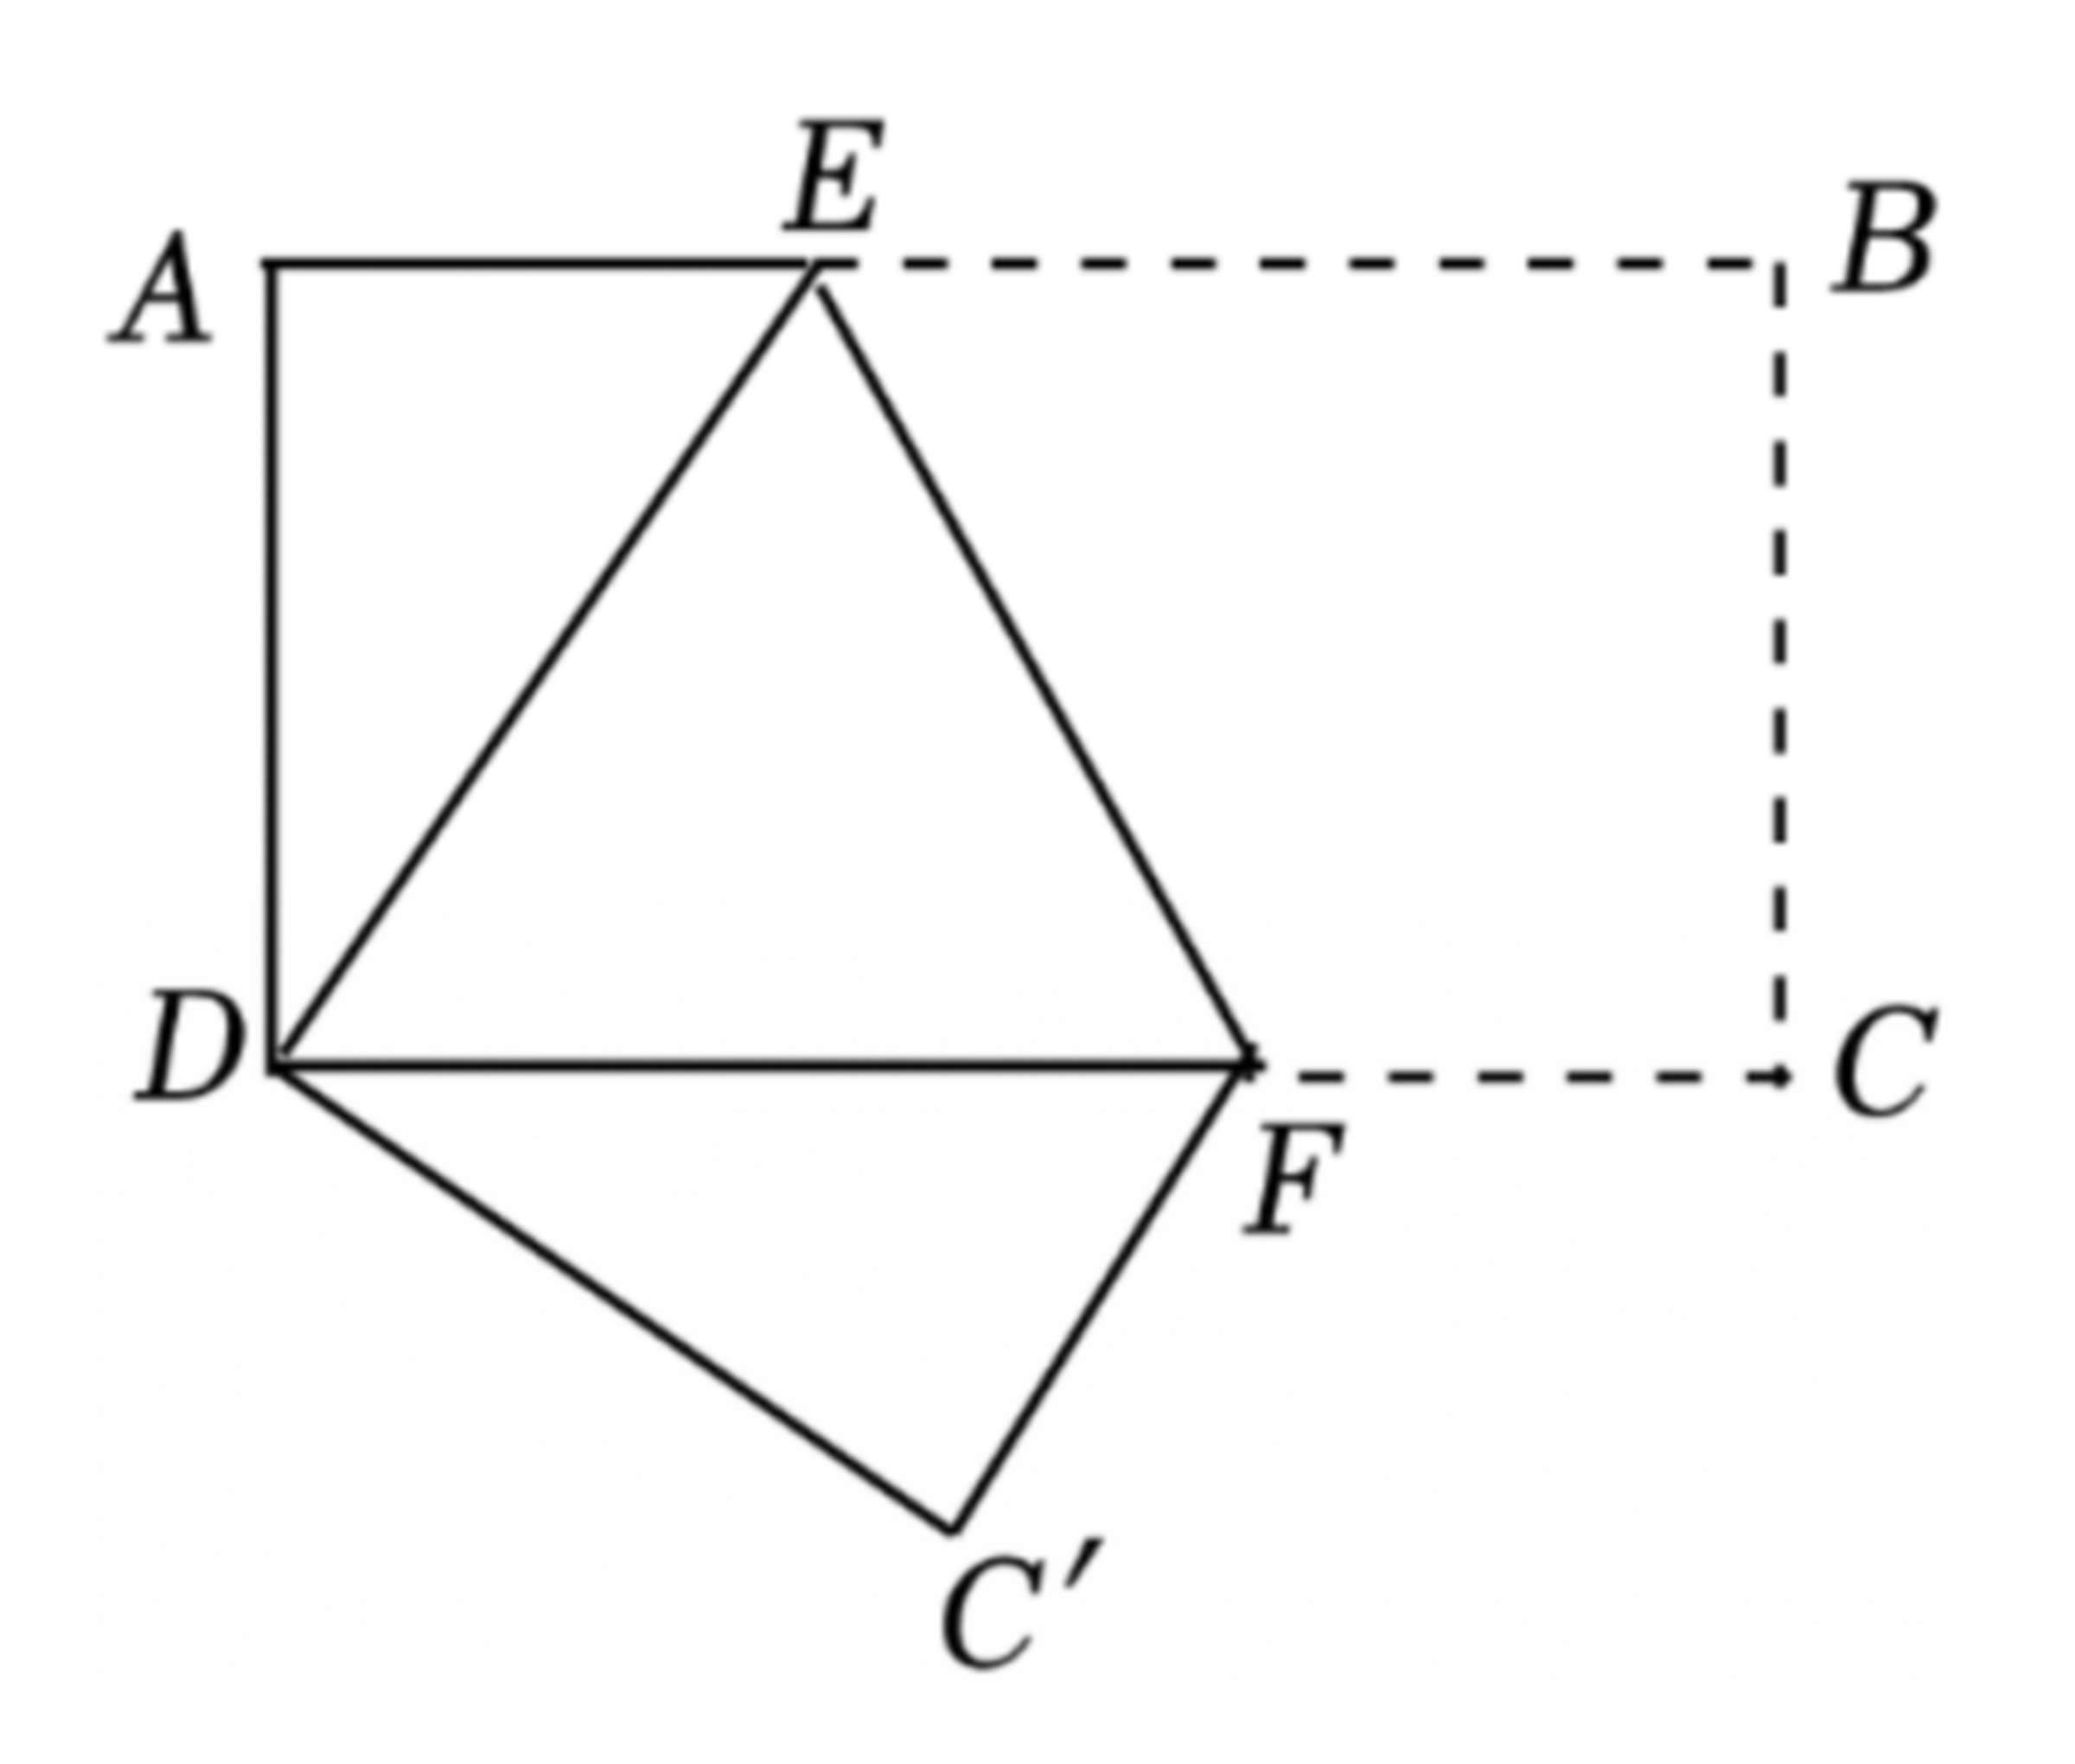
\includegraphics[width=0.40\textwidth]{figures/gao149_q11.png}
\end{center}

\ifanswer
\solbegin
\step{因为矩形 $ABCD(AB>AD)$ 的周长为 12，}
\step{在 $AB$ 和 $CD$ 边上分别取点 $E$ 和 $F$，将四边形 $BCFE$ 沿 $EF$ 折叠，}
\step{使点 $B$ 与点 $D$ 重合，此时点 $C$ 的对应点为 $C'$，}
\step{所以设 $AD=a$，$AB=b$，则 $2(a+b)=12$，}
\step{所以 $a+b=6$，且 $AB>AD$，所以 $b>a>0$，}
\step{设 $DF=x$，则 $C'F=b-x$，在 $Rt\triangle DC'F$ 中，$DC'=BC=a$，}% 几何三角形符号原卷印扁等边细线三角 $\triangle$，照录（放大 02 页确认）；$Rt$ 照录
\step{所以 $a^2+(b-x)^2=x^2$，解得 $x=\dfrac{a^2+b^2}{2b}$，}
\step{因此 $\triangle C'DF$ 的面积 $S=\dfrac{1}{2}\cdot DC'\cdot C'F=\dfrac{1}{2}\cdot a\cdot(b-x)$，}
\step{又 $b-x=b-\dfrac{(6-b)^2+b^2}{2b}=\dfrac{6(b-3)}{b}$，}
\step{所以 $S=\dfrac{1}{2}\cdot a\cdot\dfrac{6(b-3)}{b}=\dfrac{1}{2}\cdot(6-b)\cdot\dfrac{6(b-3)}{b}=\dfrac{3(6-b)(b-3)}{b}$}
\step{$=3\cdot\left(-b-\dfrac{18}{b}+9\right)$，又 $b+\dfrac{18}{b}\geqslant2\sqrt{b\cdot\dfrac{18}{b}}=6\sqrt{2}$，}
\step{当且仅当 $b=\dfrac{18}{b}$ 即 $b=3\sqrt{2}$ 时取等号，此时满足 $b>a$，}
\step{所以 $S\leqslant3\cdot(-6\sqrt{2}+9)=27-18\sqrt{2}$，故 $\triangle C'DF$ 面积的最大值为 $27-18\sqrt{2}$.}
\solend
\fi

% === Q12 === 解析内 3 幅三次函数曲线坐标图（仅答案版出）；解析 15 行（8 行 03 页＋7 行 04 页）
\item 已知 $m>0$，若存在 $t\in\R$，使得对任意 $x\in[0,m]$，不等式 $[(x-1)^2-t](x-t)\leqslant0$ 恒成立，则 $m$ 的最大值是\blankline[4.4em].

\ifanswer
\solbegin
\step{当 $t\leqslant0$ 时，$(x-1)^2-t\geqslant0$ 恒成立，}
\step{不等式 $[(x-1)^2-t](x-t)\leqslant0$ 的解集为 $x\leqslant t$，与 $x\in[0,m]$ 矛盾；}
\step{当 $t>0$ 时，不等式 $[(x-1)^2-t](x-t)\leqslant0\Leftrightarrow(x-1-\sqrt t)(x-1+\sqrt t)(x-t)\leqslant0$，}
\step{若 $t<1-\sqrt t$，即 $t\in\left(0,\dfrac{3-\sqrt5}{2}\right)$，}
\begin{center}
% 情形一 $t<1-\sqrt t$ 曲线图取 03 页右侧，去粉色水印、去色、4× LANCZOS 放大；仅答案版出
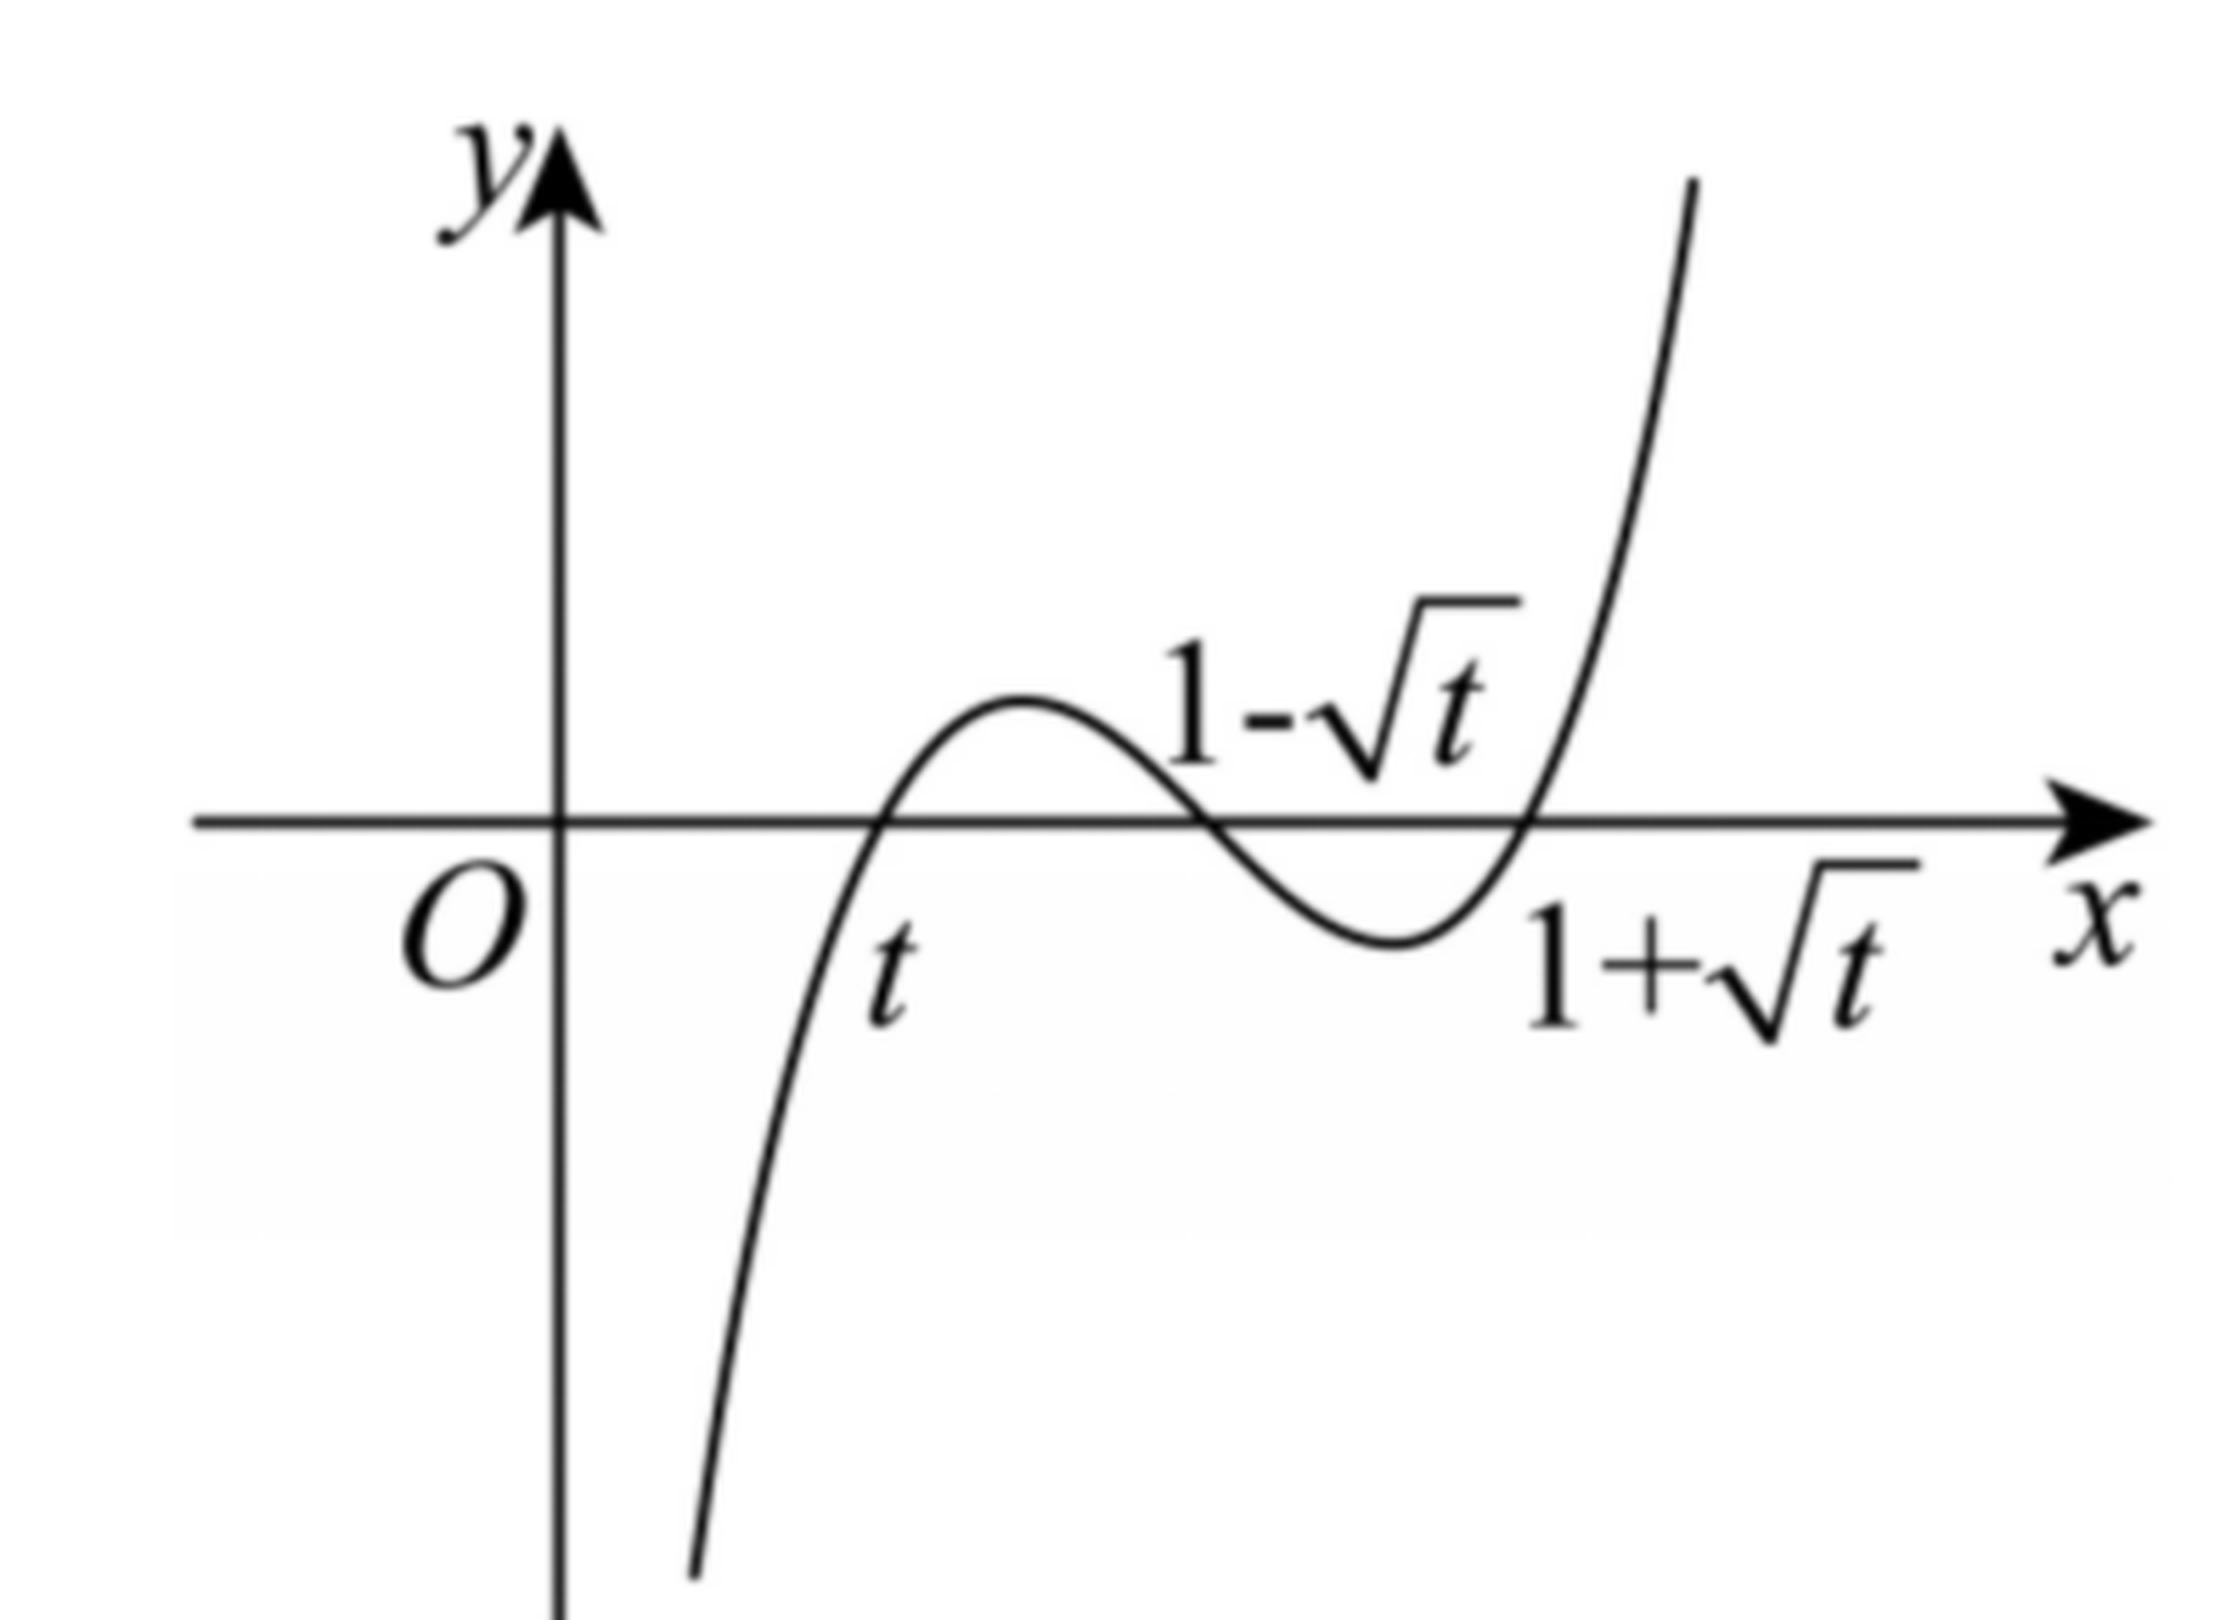
\includegraphics[width=0.40\textwidth]{figures/gao149_q12_a.png}
\end{center}
\step{则原不等式的解集为 $(-\infty,t]\cup[1-\sqrt t,1+\sqrt t]$，}
\step{当 $0<m\leqslant t$ 时，原不等式恒成立，因此}
\step{$m\in\left(0,\dfrac{3-\sqrt5}{2}\right)$；}
\step{若 $t=1-\sqrt t$，即 $t=\dfrac{3-\sqrt5}{2}$，则原不等式的解集为 $(-\infty,1+\sqrt t]$，}
\begin{center}
% 情形二 $t=1-\sqrt t$ 曲线图取 03 页右侧，去粉色水印、去色、4× LANCZOS 放大；仅答案版出
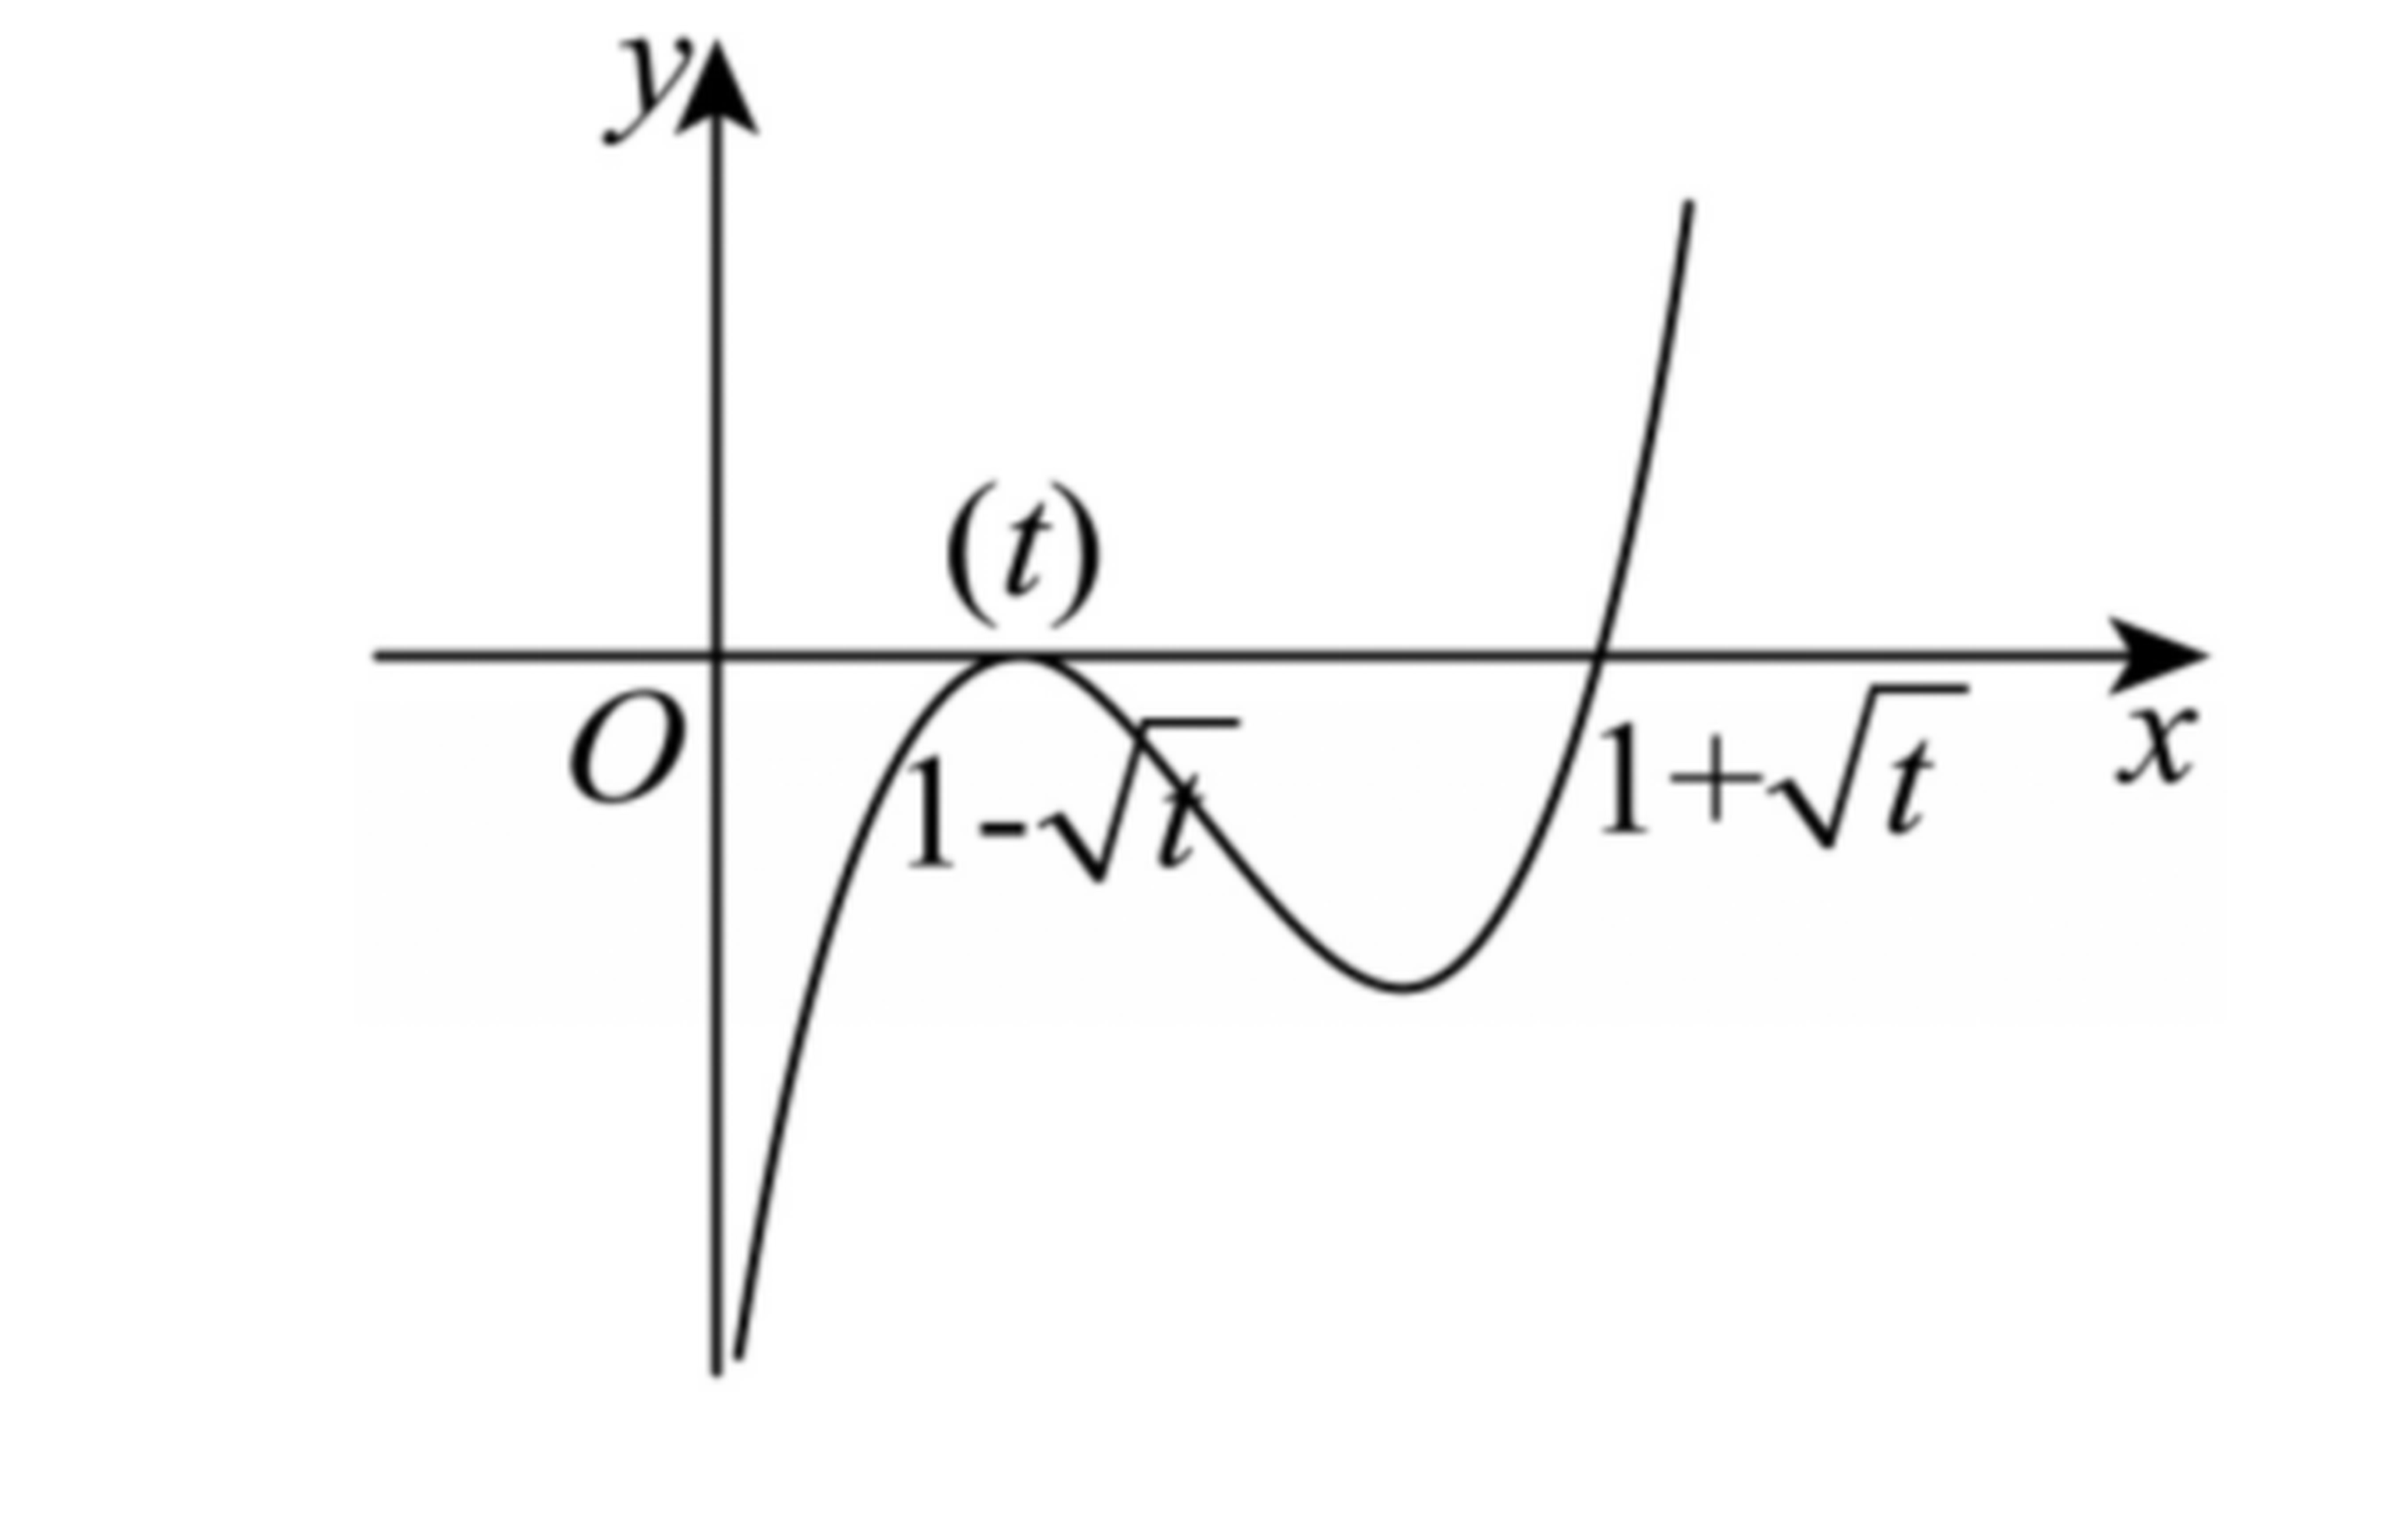
\includegraphics[width=0.40\textwidth]{figures/gao149_q12_b.png}
\end{center}
\step{当 $0<m\leqslant1+\sqrt t$ 时，原不等式恒成立，因此 $m\in\left(0,\dfrac{\sqrt5+1}{2}\right]$；}
\step{若 $1+\sqrt t>t>1-\sqrt t$，即 $t\in\left(\dfrac{3-\sqrt5}{2},\dfrac{3+\sqrt5}{2}\right)$，}
\begin{center}
% 情形三 $1+\sqrt t>t>1-\sqrt t$ 曲线图取 04 页右侧，去粉色水印、去色、4× LANCZOS 放大；仅答案版出
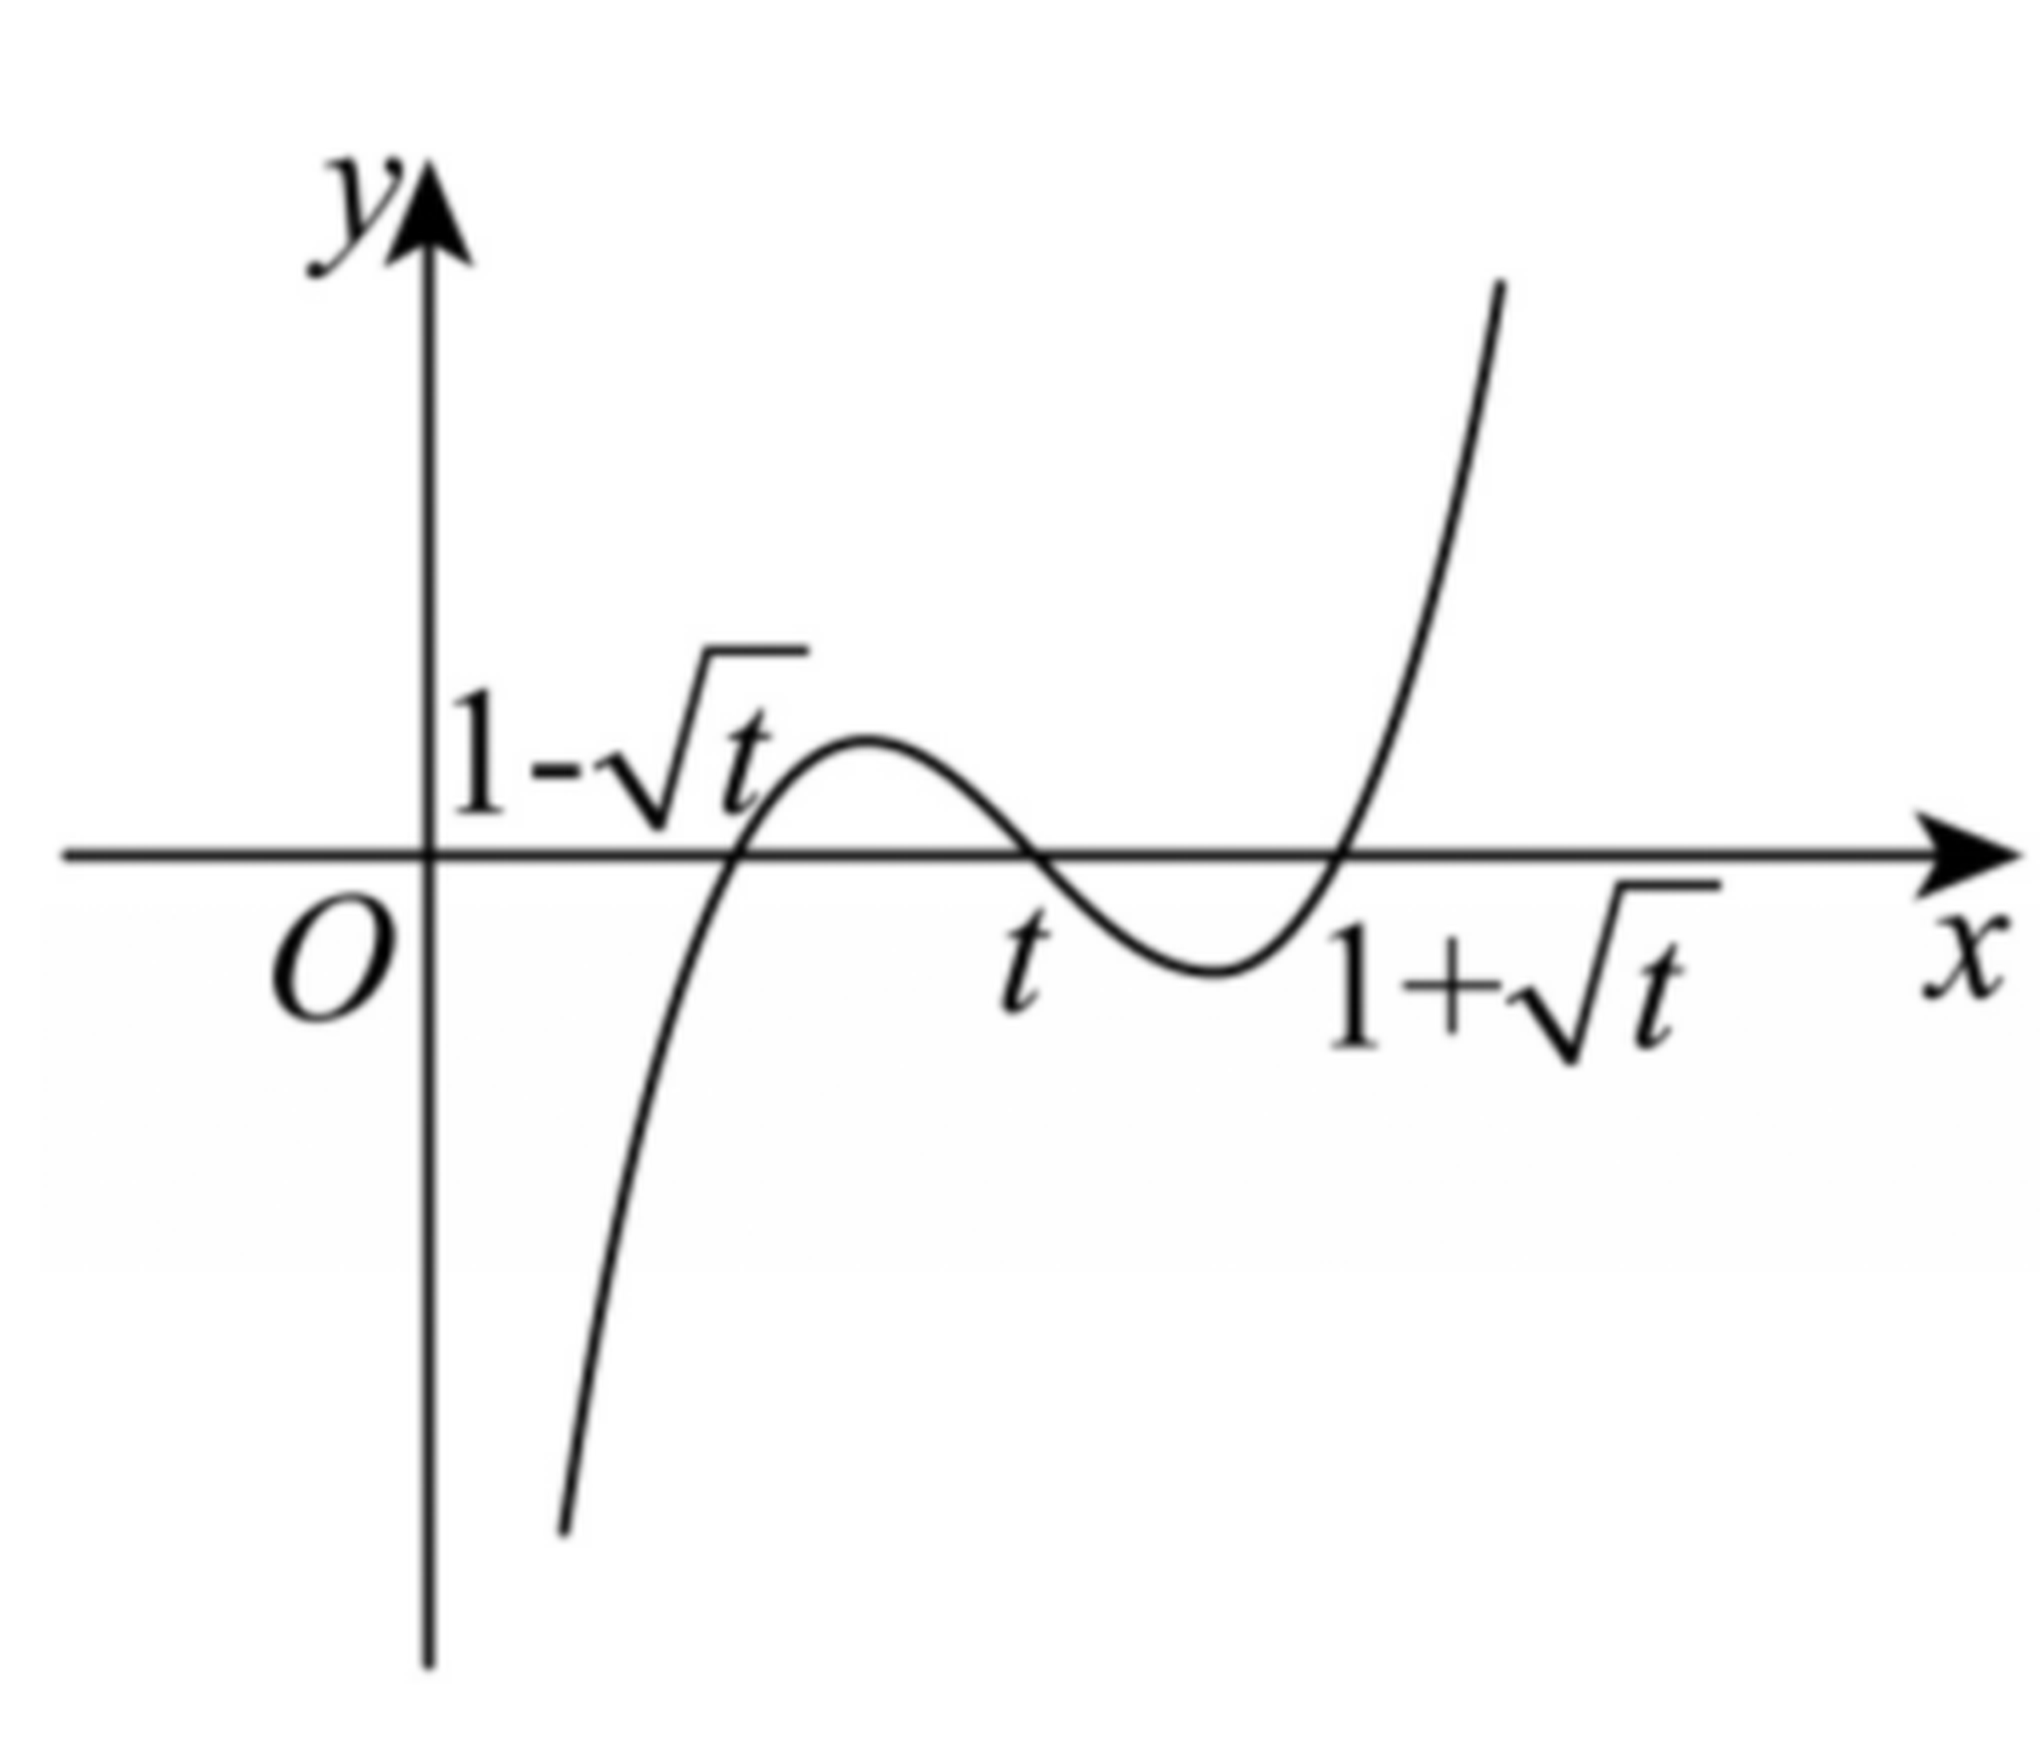
\includegraphics[width=0.40\textwidth]{figures/gao149_q12_c.png}
\end{center}
\step{则原不等式的解集为 $(-\infty,1-\sqrt t]\cup[t,1+\sqrt t]$，}
\step{当 $\begin{cases}1-\sqrt t>0\\1-\sqrt t\geqslant m\end{cases}$ 时，原不等式恒成立，此时 $t\in\left(\dfrac{3-\sqrt5}{2},1\right)$，$m\in\left(0,\dfrac{3-\sqrt5}{2}\right)$；}
\step{若 $t\geqslant1+\sqrt t$，即 $t\geqslant\dfrac{3+\sqrt5}{2}$，则取 $x=0$，$(t-1)t>0$，}
\step{原不等式不恒成立，不符合题意，}
\step{因此实数 $m$ 的取值范围是 $\left(0,\dfrac{\sqrt5+1}{2}\right]$，$m$ 的最大值是 $\dfrac{\sqrt5+1}{2}$.}
\solend
\fi

\end{enumerate}

\bigsec{二、选择题}

\begin{enumerate}
\setcounter{enumi}{12}

% === Q13 ===：答案"C"直接印在题干括号内、无【答案】/【解析】段，按 高一84 Q13／高一148 Q13 成例括号留空、另提 \ans{$C$}；四选项两行两列照原卷分行
\item 设 $ab>0$，则 $a>b$ 是 $\dfrac{1}{a}<\dfrac{1}{b}$ 的\mbox{（\quad）}

\keepwithprev
A. 充分不必要条件\qquad\qquad B. 必要不充分条件

C. 充要条件\qquad\qquad D. 既不充分又不必要条件

\ifanswer
\ans{$C$}
\fi

% === Q14 ===：$A\subset B$ 单线照录；四选项补集照原卷上划线 \overline{A}／\overline{B}；解析 1 行（由韦恩图得 B 对）
\item 已知集合 $A$、$B$ 非空，且 $A\subset B$，则下列式子中一定是空集的为\mbox{（\quad）}

\keepwithprev
A. $\overline{A}\cap B$\qquad B. $A\cap\overline{B}$\qquad C. $\overline{A}\cap\overline{B}$\qquad D. $\overline{A}\cup\overline{B}$

\ifanswer
\solbegin
\step{由韦恩图得 $B$ 对. 故选 $B$.}
\solend
\fi

% === Q15 ===："天文数字"弯引号照录；解析 2 行（首行在 04 页末、末行续 05 页顶）
\item 历史上数学计算方面的三大发明是阿拉伯数字、十进制和对数，其中对数的发明，大大缩短了计算时间，为人类研究科学和了解自然起了重大作用，对数运算对估算“天文数字”具有独特的优势. $2.5^{1000}$ 的估算值约为\mbox{（\quad）}

\keepwithprev
A. $10^{365}$\qquad B. $10^{379}$\qquad C. $10^{389}$\qquad D. $10^{398}$

\ifanswer
\solbegin
\step{$\lg 2.5^{1000}=1000\lg 2.5=1000(1-2\lg 2)\approx1000\times(1-0.602)=398$，}
\step{所以 $2.5^{1000}\approx10^{398}$. 故选 $D$.}
\solend
\fi

% === Q16 ===："完美集"新定义、圈数字①②文本模式；题干"若对任意 $x$，$y\in A$"用全角逗号、解析用顿号"$x$、$y\in A$"，两处照录不统一；解析 9 行
\item 设全集 $U=\R$，集合 $A$ 是一个非空数集，若对任意 $x$，$y\in A$，都有 $x+y\in A$、$xy\in A$，则称集合 $A$ 为一个“完美集”，给出以下命题：

①若 $A_1$、$A_2$ 都是“完美集”，且 $A_1\cap A_2\ne\varnothing$，则 $A_1\cap A_2$ 也是“完美集”；

②若 $A_1$、$A_2$ 都是“完美集”，则 $A_1\cup A_2$ 也是“完美集”.

下列说法正确的是\mbox{（\quad）}

\keepwithprev
A. ①②都是真命题\qquad\qquad B. ①是真命题，②是假命题

C. ①是假命题，②是真命题\qquad\qquad D. ①②都是假命题

\ifanswer
\solbegin
\step{由题意，全集 $U=\R$，集合 $A$ 是一个非空数集，}
\step{若对任意 $x$、$y\in A$，都有 $x+y\in A$、$xy\in A$，则称集合 $A$ 为一个“完美集”，}
\step{对于①，取 $x$、$y\in A_1\cap A_2$，则 $x\in A_1$，$x\in A_2$，$y\in A_1$，$y\in A_2$，}
\step{又 $A_1$、$A_2$ 是“完美集”，所以 $x+y\in A_1$，$xy\in A_1$，$x+y\in A_2$，$xy\in A_2$，}
\step{所以 $x+y\in A_1\cap A_2$，$xy\in A_1\cap A_2$，所以 $A_1\cap A_2$ 是“完美集”，故①正确；}
\step{对于②，取“完美集” $A_1=\{x\mid x=2k,k\in\Z\}$，$A_2=\{x\mid x=3k,k\in\Z\}$，}
\step{则 $2\in A_1$，$3\in A_2$，但 $2+3\notin A_1\cup A_2$，}
\step{即此时 $A_1\cup A_2$ 不是“完美集”，故②错误.}
\step{故选 $B$.}
\solend
\fi
\end{enumerate}

\bigsec{三、解答题}

\begin{enumerate}
\setcounter{enumi}{16}

% === Q17 ===："图像"（有亻）照录（Q17 题干与解析共 2 处）；绝对值 \lvert…\rvert；解析 7 行
\item 已知 $m\in\R$，$f(x)=(m^2-m-5)x^m$. 若 $y=f(x)$ 是幂函数，且其图像不经过原点.

(1) 求实数 $m$ 的值；

(2) 若 $f(a)=f(b)$ 且 $a\ne b$，求 $\lvert a+2\rvert+\lvert b-1\rvert$ 的最小值，并指出取到最小值时 $a$ 的取值范围.

\ifanswer
\solbegin
\step{(1) $f(x)=(m^2-m-5)x^m$ 是幂函数，得 $m^2-m-5=1$，即 $m^2-m-6=0$，}
\step{解得 $m=-2$ 或 $m=3$，又函数图像不经过原点，所以 $m=-2$($3$ 舍)；}
\step{(2) 由 (1) 得 $f(x)=x^{-2}=\dfrac{1}{x^2}$ 为偶函数，}
\step{$x<0$ 时，函数 $f(x)$ 严格增，$x>0$ 时，函数 $f(x)$ 严格减，}
\step{又 $f(a)=f(b)$ 且 $a\ne b$，所以 $a=-b$，且 $a\ne0$，$b\ne0$，}
\step{则 $\lvert a+2\rvert+\lvert b-1\rvert=\lvert a+2\rvert+\lvert-a-1\rvert=\lvert a+2\rvert+\lvert a+1\rvert$，}
\step{则 $\lvert a+2\rvert+\lvert b-1\rvert$ 的最小值为 $1$，取到最小值时 $a$ 的取值范围是 $[-2,-1]$.}
\solend
\fi

% === Q18 ===：判别式两形混用——(1) cases 块印高 \Delta、(2) 独立行印扁 \triangle，逐处照录不统一；解析 8 行
\item 已知命题 $p$：方程 $x^2+4x+m-1=0$ 有两个不等的负根；命题 $q$：方程 $4x^2+4x+m-2=0$ 无实根.

(1) 若 $p$ 为真命题，求 $m$ 的取值范围；

(2) 若 $p$、$q$ 两命题一真一假，求 $m$ 的取值范围.

\ifanswer
\solbegin
\step{(1) 若 $p$ 为真命题，即方程 $x^2+4x+m-1=0$ 有两个不等的负根；}
\step{必有 $\begin{cases}\Delta=16-4(m-1)>0\\m-1>0\end{cases}$，解得 $1<m<5$，即 $m$ 的取值范围为 $(1,5)$；}
\step{(2) 命题 $q$：方程 $4x^2+4x+m-2=0$ 无实根，}
\step{则有 $\triangle=16-16(m-2)<0$，解得 $m>3$，}
\step{若 $p$ 和 $q$ 有且只有一个为真命题，}
\step{若 $p$ 真 $q$ 假，必有 $\begin{cases}1<m<5\\m\leqslant3\end{cases}$，则有 $1<m\leqslant3$，}
\step{若 $p$ 假 $q$ 真，必有 $\begin{cases}m\leqslant1\text{ 或 }m\geqslant5\\m>3\end{cases}$，则有 $m\geqslant5$，}
\step{综上，$1<m\leqslant3$ 或 $m\geqslant5$.}
\solend
\fi

% === Q19 ===：$A\subseteq B$ 带下划线照录；解析 7 行（(2) 两组 cases 并排）
\item 已知 $m\in\R$，集合 $A=\left\{x\mid y=\sqrt{3-x}-\dfrac{1}{\sqrt{x-1}}\right\}$，集合 $B=\{x\mid 2m\leqslant x\leqslant1-m\}$.

(1) 若 $A\cup B=B$，求实数 $m$ 的取值范围；

(2) 若 $A\cap B=\varnothing$，求实数 $m$ 的取值范围.

\ifanswer
\solbegin
\step{(1) 函数 $y=\sqrt{3-x}-\dfrac{1}{\sqrt{x-1}}$，则 $\begin{cases}3-x\geqslant0\\x-1>0\end{cases}$，解得 $1<x\leqslant3$，}
\step{所以 $A=\{x\mid1<x\leqslant3\}$，}
\step{因为 $A\cup B=B$，所以 $A\subseteq B$，则 $\begin{cases}2m\leqslant1\\1-m\geqslant3\end{cases}$，解得 $m\leqslant-2$，}
\step{综上，实数 $m$ 的取值范围为 $(-\infty,-2]$；}
\step{(2) 当 $B=\varnothing$ 时，则 $2m>1-m$，解得 $m>\dfrac{1}{3}$，}
\step{当 $B\ne\varnothing$ 时，则 $\begin{cases}2m\leqslant1-m\\2m>3\end{cases}$ 或 $\begin{cases}2m\leqslant1-m\\1-m\leqslant1\end{cases}$，解得 $m\in\varnothing$ 或 $0\leqslant m\leqslant\dfrac{1}{3}$，}
\step{综上，实数 $m$ 的取值范围为 $[0,+\infty)$.}
\solend
\fi

% === Q20 ===：n 阶基本不等式推广；(3) 解析含 \overbrace{…}^{k} 上括号；(2) 解析"x=x=x=3(1-x)"三连等系原卷笔误、照录加注（见 ⑤）；解析 14 行
\item 教材中的基本不等式可以推广到 $n$ 阶：$n$ 个正数的算术平均数不小于它们的几何平均数，即对于任意的正数 $a_1$、$a_2$、$\cdots$、$a_n$，有 $\dfrac{a_1+a_2+\cdots+a_n}{n}\geqslant\sqrt[n]{a_1\cdot a_2\cdots a_n}$（$n\in\N$ 且 $n\geqslant2$），且等号当且仅当 $a_1=a_2=\cdots=a_n$ 时成立. 利用此结论解决下列问题：

(1) 若 $x$、$y$、$z>0$，求 $\dfrac{y}{x}+\dfrac{2z}{y}+\dfrac{4x}{z}$ 的最小值；

(2) 已知 $0<x<1$，求 $x^3(1-x)$ 的最大值，并求取得最大值时的 $x$ 的值；

(3) 对任意的正整数 $k$，判断 $\left(1+\dfrac{1}{k}\right)^k$ 与 $\left(1+\dfrac{1}{k+1}\right)^{k+1}$ 的大小关系，并证明.

\ifanswer
\solbegin
\step{(1) 因为 $x$、$y$、$z>0$，有 $\dfrac{y}{x}>0$，$\dfrac{2z}{y}>0$，$\dfrac{4x}{z}>0$}
\step{所以 $\dfrac{y}{x}+\dfrac{2z}{y}+\dfrac{4x}{z}\geqslant3\sqrt[3]{\dfrac{y}{x}\cdot\dfrac{2z}{y}\cdot\dfrac{4x}{z}}=3\sqrt[3]{8}=6$，}
\step{当且仅当 $\dfrac{y}{x}=\dfrac{2z}{y}=\dfrac{4x}{z}$ 时取等号，故 $\dfrac{y}{x}+\dfrac{2z}{y}+\dfrac{4x}{z}$ 的最小值为 $6$.}
\step{(2) 因为 $0<x<1$，所以 $1-x>0$，}
\step{$x^3(1-x)=\dfrac{1}{3}[x\cdot x\cdot x\cdot3(1-x)]\leqslant\dfrac{1}{3}\left[\dfrac{x+x+x+3(1-x)}{4}\right]^4=\dfrac{1}{3}\times\left(\dfrac{3}{4}\right)^4$}
\step{$=\dfrac{27}{256}$，当且仅当 $x=x=x=3(1-x)$，即 $x=3(1-x)$，$x=\dfrac{3}{4}$ 取等号，}% 原卷"x=x=x=3(1-x)"三连等，疑为四因子相等之误排，放大 08 页确认，照录未改（见 ⑤）
\step{所以 $0<x<1$ 时，$x^3(1-x)$ 的最大值是 $\dfrac{27}{256}$，取最大值时 $x=\dfrac{3}{4}$.}
\step{(3) 对任意 $k\in\N^*$，$\left(1+\dfrac{1}{k}\right)^k<\left(1+\dfrac{1}{k+1}\right)^{k+1}$.}
\step{证明：$\left(1+\dfrac{1}{k}\right)^k=\overbrace{\left(1+\dfrac{1}{k}\right)\cdot\left(1+\dfrac{1}{k}\right)\cdots\left(1+\dfrac{1}{k}\right)}^{k}\times1$}
\step{$\leqslant\left(\dfrac{\overbrace{\left(1+\dfrac{1}{k}\right)+\left(1+\dfrac{1}{k}\right)+\cdots+\left(1+\dfrac{1}{k}\right)}^{k}+1}{k+1}\right)^{k+1}$}
\step{$=\left(\dfrac{\overbrace{(1+1+\cdots+1)}^{k}+\overbrace{\left(\dfrac{1}{k}+\dfrac{1}{k}+\cdots+\dfrac{1}{k}\right)}^{k}+1}{k+1}\right)^{k+1}=\left(\dfrac{k+1+1}{k+1}\right)^{k+1}=\left(1+\dfrac{1}{k+1}\right)^{k+1}$，}
\step{当且仅当 $1+\dfrac{1}{k}=1$ 时取等号，}
\step{但是任意 $k\in\N^*$ 时 $1+\dfrac{1}{k}>1$，所以等号不成立，}
\step{故任意 $k\in\N^*$ 时，$\left(1+\dfrac{1}{k}\right)^k<\left(1+\dfrac{1}{k+1}\right)^{k+1}$.}
\solend
\fi

% === Q21 ===："减 k 集"新定义（引号内 k／数字两侧空格照录）；解析 26 行（续 10 页），含 ⑤ 三处原卷笔误照录
\item 定义：对于给定的整数 $k$，若非空集合 $A$ 满足如下 3 个条件：

① $A$ 是正整数集的子集；② $A\ne\{1\}$；

③对任意正整数 $x,y$，若 $x+y\in A$，则 $xy-k\in A$；则称集合 $A$ 为“减 $k$ 集”.

(1) 判断集合 $A=\{1,2\}$ 是否为“减 $0$ 集”？是否为“减 $1$ 集”？（无需说明理由）

(2) 证明：不存在“减 $2$ 集”；

(3) 是否存在“减 $1$ 集”？如果存在，求出所有“减 $1$ 集”；如果不存在，说明理由.

\ifanswer
\solbegin
\step{(1) 因为 $P\subseteq\N^*$，$P\ne\{1\}$，$1+1=2\in P$，$1\times1-0\in P$，}
\step{所以集合 $P=\{1,2\}$ 是“减 $0$ 集”；}
\step{因为 $P\subseteq\N^*$，$P\ne\{1\}$，$1+1=2\in P$，$1\times1-1\notin P$，}
\step{所以集合 $P=\{1,2\}$ 是“减 $1$ 集”；}% 按条件③应为"不是"，原卷径印"是"，放大 09 页确认，照录未改（见 ⑤）
\step{(2) 假设存在集合 $A$ 是“减 $2$ 集”，若 $x+y\in A$，则 $xy-2\in A$，}
\step{①当 $x+y=xy-2$ 时，有 $(x-1)(y-1)=3$，}
\step{则 $x$、$y$ 一个为 $2$，一个为 $4$，所以集合 $A$ 有元素 $6$，}
\step{但 $3+3\in A$，$3\times3-2\notin A$，与 $A$ 是“减 $2$ 集”矛盾；}
\step{②当 $x+y\ne xy-2$ 时，则 $x+y=xy-1$ 或 $x+y=xy-m$($m>2$)，}
\step{若 $x+y=xy-1$，$m=1$ 时，$M$ 为除 $1$ 以外的最小元素，}% 原卷"m=1"上文未显式定义，疑笔误，放大 09 页确认，照录未改（见 ⑤）
\step{则 $x=M-1$，$y=1$ 时，$xy-2=M-3$ 小于 $M$，}
\step{要符合题意，必须 $M=4$，}
\step{此时取 $x-2$，$y=2$，$xy-2=2$ 不属于 $A$，故不符合题意，}% 原卷"取 x−2"疑为"取 x=2"误排，放大 09 页确认，照录未改（见 ⑤）
\step{当 $m>2$ 时，$(x-1)(y-1)=m+1$，同样得出矛盾，}
\step{综上，不存在 $A$ 是“减 $2$ 集”.}
\step{(3) 存在“减 $1$ 集” $A$，则 $A\ne\{1\}$，}
\step{①假设 $1\in A$，则 $A$ 中除了元素 $1$ 以外，必然还含有其它元素，}
\step{假设 $2\in A$，$1+1\in A$，而 $1\times1-1\notin A$，所以 $2\notin A$，}
\step{假设 $3\in A$，$1+2\in A$，而 $1\times2-1\in A$，所以 $3\in A$，}
\step{所以 $A=\{1,3\}$，}
\step{假设 $4\in A$，$1+3\in A$，而 $1\times3-1\notin A$，所以 $4\notin A$，}
\step{假设 $5\in A$，$1+4\in A$，$1\times4-1\in A$，$2+3=5$，$2\times3-1\in A$，所以 $5\in A$，}
\step{所以 $A=\{1,3,5\}$，}
\step{以此类推，得 $A=\{1,3,5,\cdots,2n-1,\cdots\}$，($n\in\N^*$)，}
\step{所以所有的“减 $1$ 集”有 $\{1,3\}$，$\{1,3,5\}$，$\{1,3,5,7\}$，$\cdots$，$\{1,3,5,\cdots,2n-1,\cdots\}$，}
\step{$(n\in\N^*)$.}
\solend
\fi
\end{enumerate}

\end{document}
"
% 紧凑版：xelatex "\def\iscompact{1}% 高一149_青浦高级中学上外云间_期中.tex
%   —— 高一上数学"2026-2027 年青浦高级中学上外云间高一上期中"（试卷版/答案版/紧凑版）
% 试卷版：xelatex 高一149_青浦高级中学上外云间_期中.tex
% 答案版：xelatex "\def\isanswer{1}% 高一149_青浦高级中学上外云间_期中.tex
%   —— 高一上数学"2026-2027 年青浦高级中学上外云间高一上期中"（试卷版/答案版/紧凑版）
% 试卷版：xelatex 高一149_青浦高级中学上外云间_期中.tex
% 答案版：xelatex "\def\isanswer{1}% 高一149_青浦高级中学上外云间_期中.tex
%   —— 高一上数学"2026-2027 年青浦高级中学上外云间高一上期中"（试卷版/答案版/紧凑版）
% 试卷版：xelatex 高一149_青浦高级中学上外云间_期中.tex
% 答案版：xelatex "\def\isanswer{1}\input{高一149_青浦高级中学上外云间_期中.tex}"
% 紧凑版：xelatex "\def\iscompact{1}\input{高一149_青浦高级中学上外云间_期中.tex}"
%
% ① 原始材料：微信公众号"魔都数学加油站"文章，连载"27学年高一149"，原文标题
% "27学年高一149——2026-2027年上海市青浦高级中学上外云间高一上期中"；
% 原文链接：https://mp.weixin.qq.com/s/T7_nyoR1k0o_5og7FkDsyw 。
% 正文为 10 张 PNG 页（01/02/03/04/10 为 2560×3620，05/06/07/08/09 为 4762×6735，
% 同一篇各页分辨率混排，逐页按各自分辨率裁图核对，别按预览比例换算裁框）。
% 体例：混合体例讲评版——19 题中 Q6 只印【答案】、无【解析】；Q13 的答案"C"
%   直接印在题干括号内、无【答案】/【解析】段；其余 17 题印【解析】（逐题核实，见 ② ②）。
% 题目、答案、解析均据原图转录；卷面粉红色水印"魔都数学加油站"及公众号页脚未录入。
% 全卷插图清单（逐页通读 10 页确认）：1 幅题目配图 + 3 幅【解析】内配图：
%   · Q11 矩形 ABCD 折叠几何图（02 页右侧：A/B/C/D/E/F/C' 与虚线 EB、BC、FC），
%     题干"如图"处，题目配图、三版都出，裁 figures/gao149_q11.png；
%   · Q12【解析】内 3 幅三次函数曲线坐标图（03 页右侧两幅 + 04 页右侧一幅：
%     x/y 轴、O、t、1-\sqrt t、1+\sqrt t 等标注，分别对应 t<1-\sqrt t、
%     t=1-\sqrt t、1+\sqrt t>t>1-\sqrt t 三种情形），解析配图、仅答案版出，
%     分别裁 figures/gao149_q12_a.png／_b.png／_c.png，放 \ifanswer 内 \step 之间
%     （高一73 第 16 题成例）；
%   其余各页逐页确认无其它题目配图、无表格；Q14 解析"由韦恩图得 B 对"仅文字推导、
%   原卷并未印韦恩图；Q9／Q18／Q19 的 cases 块与 Q20(3) 的 \overbrace 为数学块（非图）；
%   10 页下半仅水印、无正文。4 图均取自原卷截图，去粉色水印、去色、4× LANCZOS 放大。
%
% 卷首标题：原卷印作"2026-2027 年青浦高级中学上外云间高一上期中"，年份区间按全稿
% 惯例排 en dash；原卷卷面未印副标题，本稿按同期中卷（高一140／141／143／144／145／
% 146／147／148）知识模块口径补出"集合与常用逻辑用语、不等式、函数"。
%
% 题号体例（逐页核实定稿）：本卷共 19 题——一、填空题 3—12（10 题）、
% 二、选择题 13—16（4 题）、三、解答题 17—21（5 题）。
% 三节分别 \setcounter{enumi}{2}／{12}／{16}。原卷从第 3 题起、无第 1、2 题，
% 本稿保留原题号；全卷无附加题节（Q21 解析末行"（n\in N^*）."为全卷收尾）。
%
% ② 与原卷的排版差异：
%   ① 原文从第 3 题起，本稿保留原题号；共 19 题三节；
%   ② 混合体例逐题核实：Q6（反证法"假设的内容"）只印【答案】、无【解析】，
%      按 高一140 第 5 题／高一145 Q3 成例提 \ans{}、不补造解析；Q13 答案"C"直接
%      印在题干括号内、全卷无该题【答案】/【解析】段，按 高一84 Q13／高一148 Q13
%      成例括号 \mbox{（\quad）} 留空、另提 \ans{$C$}；其余 17 题印【解析】、
%      用 \solbegin…\solend，选择题答案在解析末句"故选 X"（Q14 选 B、Q15 选 D、
%      Q16 选 B，逐个放大 04/05 页核实）、题干括号留空、不另提 \ans{}；
%      答案版【答案】/【解析】标记数 = 19（2 个 \ans ＋ 17 个 \solbegin）
%      = 全卷题数；
%   ③ 原卷卷面未印副标题，本稿按知识模块口径补出；
%   ④ 原卷填空横线按全稿惯例排 \blankline[4.4em]；选择题括号排 \mbox{（\quad）}、
%      选项段前按惯例加 \keepwithprev；Q13／Q16 四选项为两行两列、Q14／Q15
%      选项为一行，照原卷分行；解答题不留作答区、不加 \anspace（原卷为讲评版）；
%   ⑤ 数集：Q6"a,b\in N"、Q8"x\in R"、Q9"a\in R"／"解集为 R"、Q12"t\in R"、
%      Q16"U=R"、Q17"m\in R"、Q19"m\in R"、Q20"n\in N" 原卷印斜体 R/N，
%      按全稿惯例统一改 \R／\N；Q20(3)、Q21 的 $N^*$ 排 \N^*；Q16 解析
%      "$k\in Z$" 排 \Z。绝对值排 \lvert…\rvert（Q17），集合描述竖线排 \mid
%      （Q19、Q16 解析）；不等号按全稿惯例排 \leqslant／\geqslant；
%      补集照原卷上划线排 \overline{A}／\overline{B}（Q14 四选项）；空集
%      \varnothing（Q16、Q19、Q21）；
%   ⑥ 子集符号逐处照录不统一：Q4 题干"{1,2}⊆A⊂{1,2,3,4,5,6}" 前者印带下划线
%      ⊆、照录 \subseteq，后者印单线 ⊂、照录 \subset；Q10"A⊆{-1,1/2,2,3}"、
%      Q19 解析"A⊆B"、Q21 解析"P⊆N*" 均印带下划线 ⊆、照录 \subseteq；
%      Q14"A⊂B" 印单线 ⊂、照录 \subset（逐处放大 01/02/04/07/09 页确认，见 ④）；
%   ⑦ 子题标号 (1)(2)(3) 半角括号照录；圈数字 ①②③ 在文本模式（Q16 两命题、
%      Q21 三个条件与解析的①②）按 common.sty 划入 CJK 字符类渲染；cases 块整体
%      算一个印刷行；\left…\right 不得拆到不同 $…$ 组；数学式内 CJK 用 \text{}
%      （Q18 解析 cases 块"\text{或}"）；Q11 解析"Rt\triangle DC'F" 的 Rt 照录；
%   ⑧ 题干／解析中的中文弯引号按原卷照录：Q6" 已知 a,b\in N，若 ab 能被 5 整除，
%      那么 a、b 中至少有一个能被 5 整除 "（开引号后紧跟"已知"、闭引号后空格接"时"）、
%      Q15"天文数字"、Q16"完美集"、Q21"减 k 集""减 0 集""减 1 集""减 2 集"
%      （引号内 k／数字两侧有空格），注释内一律 ASCII 引号；
%   ⑨ 半角逗号在数学组之间是全稿惯例、非笔误（Q8"$a>0,a\ne1,x\in\R$"、
%      Q21 题干"$x,y$" 等），逐处照录别改；Q16 题干"若对任意 $x$，$y\in A$"
%      用全角逗号而解析用顿号"$x$、$y\in A$"，两处不同均照录；行末西文句点
%      照录为 ASCII `.`；行中全角逗号／顿号照录；
%   ⑩ "图像／图象"逐处放大核：Q10 题干与解析共 6 处均印"图象"（象，无亻）；
%      Q17 题干"其图像不经过原点"与解析"又函数图像不经过原点" 2 处印"图像"
%      （像，有亻），逐处照录未统一改动（放大 02/05/06 页确认）；
%   ⑪ 判别式 Δ/△ 混用是照录项：Q9 解析 cases 块"Δ=4(a−2)²+16(a−2)<0"、
%      Q18(1) cases 块"Δ=16−4(m−1)>0" 两处印等腰偏高粗三角 \Delta；
%      Q18(2) 独立行"△=16−16(m−2)<0" 印扁等边细线三角 \triangle，
%      逐处放大判断、照录不统一（参照 高一142／144／145／146／148 头注④口径）；
%      另 Q11 题干"△C'DF 面积"与解析 3 处"△"（含"Rt△DC'F"）共 4 处几何
%      三角形符号亦印扁细线三角，照录 \triangle（非判别式，字形同类，见 ④）；
%   ⑫ 一条 \step = 原卷解析的一个印刷行，cases 块整体算一个印刷行；别把原卷折行
%      并起来、别把一行拆多条。Q11 十三行（7 行在 02 页＋6 行在 03 页）、
%      Q12 十五行（8 行在 03 页＋7 行在 04 页）、Q16 九行、Q21 二十六行
%      （续 10 页）均按印刷行逐条断，不丢行；
%   ⑬ 配图：Q11 题目配图（三版都出）放 \item 内题干之后 \begin{center}，
%      大图块加 \needvspace{8cm} 守卫把整块推走（守卫放 \item 之前，见
%      高一145 Q14/Q20 成例与切页审计 B 类坑）；Q12 三幅解析配图（仅答案版出）
%      放 \ifanswer 内 \solbegin…\solend 的 \step 之间；三版切页审计均"合计异常：无"；
%   ⑭ 跨页续印按题合并：Q3/4/5 在 01 页；Q6/7/8 题干与解析在 01 页；
%      Q9 题干在 01 页末、解析 4 行在 02 页顶；Q10 题干＋解析在 02 页；
%      Q11 题干＋图＋解析前 7 行在 02 页、解析后 6 行续 03 页顶；
%      Q12 题干＋解析首行在 03 页末、解析续 7 行在 03 页下半＋7 行在 04 页顶，
%      "二、选择题"标题在 04 页下半；Q13/14 题干＋选项＋Q14 解析在 04 页下半；
%      Q15 题干＋选项＋解析首行在 04 页末、末行"所以 2.5^1000≈10^398. 故选 D."
%      续 05 页顶；Q16 题干＋选项＋解析 9 行在 05 页、"三、解答题"标题＋
%      Q17 题干首句在 05 页末；Q17(2)＋解析 7 行、Q18 题干＋解析前 6 行在 06 页；
%      Q18 解析末 2 行续 07 页顶；Q19 题干＋解析 4 行在 07 页上半、
%      解析续 3 行在 07 页下半；Q20 题干(1) 在 07 页末、题干(2)(3)＋解析(1)(2)
%      在 08 页上半、(3) 解析含 \overbrace 的证明在 08 页下半、末行
%      "故任意 k∈N* 时…"续 09 页顶；Q21 题干＋解析(1)(2)(3) 前段在 09 页、
%      解析(3) 后半 9 行续 10 页上半（10 页下半仅水印、无正文）。
%      本稿按题连排，不丢行、不并折行；
%   ⑮ 原卷解析内无红色"法一／法二"之类小标题，故本卷无 \stepm；水印
%      "魔都数学加油站"红色不录入。
%
% ③ 行数复核：一条 \step／\stepm = 原卷解析的一个印刷行，cases 块作一个印刷行计。
%   逐题数（主会话逐页核对定稿）：Q3：1；Q4：2；Q5：2；Q6：0（只印【答案】、
%   提 \ans{}）；Q7：1；Q8：1；Q9：4；Q10：5；Q11：13；Q12：15；
%   Q13：0（答案印在题干括号内、另提 \ans{}）；Q14：1；Q15：2；Q16：9；
%   Q17：7；Q18：8；Q19：7；Q20：14；Q21：26。
%   合计 118 条 \step（本卷无 \stepm：解析内无红色"法一／法二"类小标题），
%   与原卷逐题印刷行相等。全卷 17 题设 \solbegin…\solend ＋ 2 处 \ans{}，
%   答案版【答案】/【解析】标记数 = 19 = 全卷题数。
%
% ④ 判别式／子集符号结论（逐处放大原图照录、不得统一，主会话像素级复核）：
%   判别式全卷 3 处，两形混用逐处照录不统一（参照 高一142／144／145／146／148 头注④）：
%     · Q9 解析 cases 块"Δ=4(a−2)²+16(a−2)<0" 原卷印等腰偏高粗三角（高>宽、
%       粗笔画），照录 \Delta（放大 02 页 /tmp/gao149/z/t02_q9_delta2.png 确认）；
%     · Q18(1) cases 块"Δ=16−4(m−1)>0" 原卷印等腰偏高粗三角（高>宽、粗笔画），
%       照录 \Delta（放大 06 页 /tmp/gao149/z/t06_q18a.png 确认）；
%     · Q18(2) 独立行"△=16−16(m−2)<0" 原卷印扁等边细线三角（宽>高、细线），
%       照录 \triangle（放大 06 页 /tmp/gao149/z/t06_q18b.png 与 Q18(1) 并排确认）。
%   另 Q11 题干"△C'DF"与解析 3 处"△"（含"Rt△DC'F"）共 4 处几何三角形符号
%     亦印扁等边细线三角，照录 \triangle（放大 02 页
%     /tmp/gao149/z/t02_q11_tri2.png 确认），与 Q9／Q18(1) 判别式 \Delta 两形不统一。
%   子集／补集：Q4 题干"{1,2}⊆A⊂{1,2,3,4,5,6}" 前者带下划线 ⊆、照录 \subseteq，
%     后者单线 ⊂、照录 \subset（放大 01 页 /tmp/gao149/z/t01_q3q4.png 确认）；
%     Q10"A⊆{-1,1/2,2,3}"、Q19 解析"A⊆B"、Q21 解析"P⊆N*" 三处带下划线 ⊆、
%     照录 \subseteq；Q14"A⊂B" 单线 ⊂、照录 \subset（放大 04 页
%     /tmp/gao149/z/t04_q14_sub2.png 确认）；Q14 四选项补集 \overline{A}／\overline{B}
%     照原卷上划线；空集 \varnothing（Q16、Q19、Q21）；Q19／Q16 解析集合描述竖线
%     \mid；数集 \R／\N／\N^*／\Z 归一见 ② ⑤。
%
% ⑤ 存疑照录（放大原图确认，照录未改、正文对应处另有 % 注）：
%   1. Q21 解析(1) 第二组"因为 P⊆N*，P≠{1}，1+1=2∈P，1×1−1∉P，所以集合
%      P={1,2} 是"减 1 集"" —— 按条件③（x=y=1 时 xy−1=0 须∈P）应为"不是"，
%      原卷却径印"是"，放大 09 页 /tmp/gao149/z/t09_q21_sol1.png 确认，照录未改
%      （疑为原卷结论笔误）。
%   2. Q21 解析(2)"此时取 x−2，y=2，xy−2=2 不属于 A" —— 按上下文应为
%      "取 x=2"（x−2 疑为 x=2 的误排），放大 09 页
%      /tmp/gao149/z/t09_q21_sol2.png 确认，照录未改。
%   3. Q21 解析(2)"若 x+y=xy−1，m=1 时，M 为除 1 以外的最小元素" 中 $m=1$
%      上文未显式定义 m（仅"x+y=xy−m(m>2)"中出现），放大 09 页确认，照录未改。
%   4. Q20 解析(2)"当且仅当 x=x=x=3(1−x)" 三个 x 连等，疑为原卷排印（应为
%      四个因子 x,x,x,3(1−x) 相等），放大 08 页
%      /tmp/gao149/z/t08_q20_sol2.png 确认，照录未改。
%   5. Q6 只印【答案】、Q13 答案印题干括号内，两题均无【解析】，按成例提
%      \ans{}、未补造解析（见 ② ②）。
%   6. 判别式 Q9／Q18(1) 高 \Delta 与 Q18(2)／Q11 扁 \triangle 两形混用，逐处
%      照录不统一（见 ④）；"图像／图象" Q10 用"图象"、Q17 用"图像"，
%      逐处照录未统一（见 ② ⑩）。
%   全卷除此 6 类外未发现其它笔误／自相矛盾处。
%
% ⑥ 跨页续印按题合并说明：见 ② ⑭。
%
\documentclass[a4paper,11pt]{article}
\usepackage{common}

\begin{document}

\examtitlest[3]{2026--2027 年青浦高级中学上外云间高一上期中}{集合与常用逻辑用语、不等式、函数}

\bigsec{一、填空题}

\begin{enumerate}
\setcounter{enumi}{2}

% === Q3 === 根式化分数指数幂；解析 1 行
\item 根式 $\sqrt{a\sqrt a}$ 化成分数指数幂是\blankline[4.4em].

\ifanswer
\solbegin
\step{$\sqrt{a\sqrt a}=\sqrt{a\cdot a^{\frac{1}{2}}}=\sqrt{a^{1+\frac{1}{2}}}=\sqrt{a^{\frac{3}{2}}}=a^{\frac{3}{2}\times\frac{1}{2}}=a^{\frac{3}{4}}$.}
\solend
\fi

% === Q4 === 题干两种子集符号逐处照录（\subseteq 带下划线／\subset 单线）；解析 2 行
\item 满足 $\{1,2\}\subseteq A\subset\{1,2,3,4,5,6\}$ 的集合 $A$ 共有\blankline[4.4em]个.

\ifanswer
\solbegin
\step{集合 $A$ 满足 $\{1,2\}\subseteq A\subset\{1,2,3,4,5,6\}$，}% 前者带下划线 $\subseteq$、后者单线 $\subset$，逐处照录不统一（放大 01 页确认）
\step{所以集合 $A$ 的个数为集合 $\{3,4,5,6\}$ 的真子集的个数，即为 $2^4-1=15$ 个.}
\solend
\fi

% === Q5 === 解析 2 行
\item 不等式 $\dfrac{2x+1}{x-1}\leqslant0$ 的解集为\blankline[4.4em].

\ifanswer
\solbegin
\step{不等式 $\dfrac{2x+1}{x-1}\leqslant0$ 可化为 $(2x+1)(x-1)\leqslant0$，且 $x-1\ne0$，解得 $-\dfrac{1}{2}\leqslant x<1$，}
\step{即原不等式的解集为 $\left[-\dfrac{1}{2},1\right)$.}
\solend
\fi

% === Q6 === 原卷只印【答案】、无【解析】，按 高一140 第 5 题／高一145 Q3 成例提 \ans{}、不补造解析；弯引号与空格照录
\item 用反证法证明命题 “已知 $a,b\in\N$，若 $ab$ 能被 5 整除，那么 $a$、$b$ 中至少有一个能被 5 整除” 时，假设的内容应该是\blankline[4.4em].

\ifanswer
\ans{$a$、$b$ 都不能被 5 整除}
\fi

% === Q7 === 解析 1 行
\item 若 $\log_3(\log_4 x)=1$，则 $x=$\blankline[4.4em].

\ifanswer
\solbegin
\step{$\log_3(\log_4 x)=1$，则 $\log_4 x=3$，故 $x=64$.}
\solend
\fi

% === Q8 === 半角逗号在数学组之间照录；解析 1 行
\item 已知 $a>0,a\ne1,x\in\R$，且 $a^{2x}=2$，则 $\dfrac{a^{3x}+a^{-3x}}{a^x+a^{-x}}$ 的值为\blankline[4.4em].

\ifanswer
\solbegin
\step{$\dfrac{a^{3x}+a^{-3x}}{a^x+a^{-x}}=a^{2x}-1+a^{-2x}=2-1+\dfrac{1}{2}=\dfrac{3}{2}$.}
\solend
\fi

% === Q9 === 题干在 01 页末、解析 4 行在 02 页顶；cases 块整体算 1 行；判别式高 \Delta
\item 已知 $a\in\R$，若关于 $x$ 的不等式 $(a-2)x^2+2(a-2)x-4<0$ 的解集为 $\R$，则实数 $a$ 的取值范围是\blankline[4.4em].

\ifanswer
\solbegin
\step{当 $a=2$ 时，不等式化为 $-4<0$ 对于任意实数 $x$ 都成立，因此 $a=2$ 满足题意；}
\step{当 $a\ne2$ 时，要使关于 $x$ 的不等式 $(a-2)x^2+2(a-2)x-4<0$ 的解集为 $\R$，}
\step{则 $\begin{cases}a-2<0\\\Delta=4(a-2)^2+16(a-2)<0\end{cases}$，解得 $-2<a<2$.}% cases 块整体算一个印刷行；判别式原卷印等腰偏高粗三角 $\Delta$，照录（放大 02 页确认）
\step{综上，$a$ 的取值范围为 $(-2,2]$.}
\solend
\fi

% === Q10 === "图象"（象，无亻）逐处照录；\subseteq 带下划线；解析 5 行
\item 已知集合 $A=\{\alpha,\beta\}$，且 $A\subseteq\left\{-1,\dfrac{1}{2},2,3\right\}$，函数 $f(x)=x^\alpha$ 与 $g(x)=x^\beta$ 的图象有两个交点，则满足条件的不同集合 $A$ 有\blankline[4.4em]个.

\ifanswer
\solbegin
\step{函数 $y=x^{-1}$ 与 $y=x^{\frac{1}{2}}$，$y=x^2$，$y=x^3$ 的图象分别有 1 个，1 个，2 个交点；}
\step{函数 $y=x^{\frac{1}{2}}$ 与 $y=x^2$，$y=x^3$ 的图象都有 2 个交点；}
\step{函数 $y=x^2$ 与 $y=x^3$ 的图象有 2 个交点，}
\step{函数 $f(x)=x^\alpha$ 与 $g(x)=x^\beta$ 的图象若只有 2 个交点，}
\step{则 $A=\{-1,3\}$ 或 $\left\{\dfrac{1}{2},2\right\}$ 或 $\left\{\dfrac{1}{2},3\right\}$ 或 $\{2,3\}$，有 4 个.}
\solend
\fi

% === Q11 === 题目配图（矩形折叠，三版都出）；\needvspace{8cm} 守卫放 \item 之前；解析 13 行（7 行 02 页＋6 行 03 页）
\needvspace{8cm}
\item 如图，矩形 $ABCD(AB>AD)$ 的周长为 12，在 $AB$ 和 $CD$ 边上分别取点 $E$ 和 $F$，将四边形 $BCFE$ 沿 $EF$ 折叠，使点 $B$ 与点 $D$ 重合，此时点 $C$ 的对应点为 $C'$，则 $\triangle C'DF$ 面积的最大值为\blankline[4.4em].

\begin{center}
% 矩形 ABCD 折叠几何图取 02 页右侧，去粉色水印、去色、4× LANCZOS 放大；三版都出
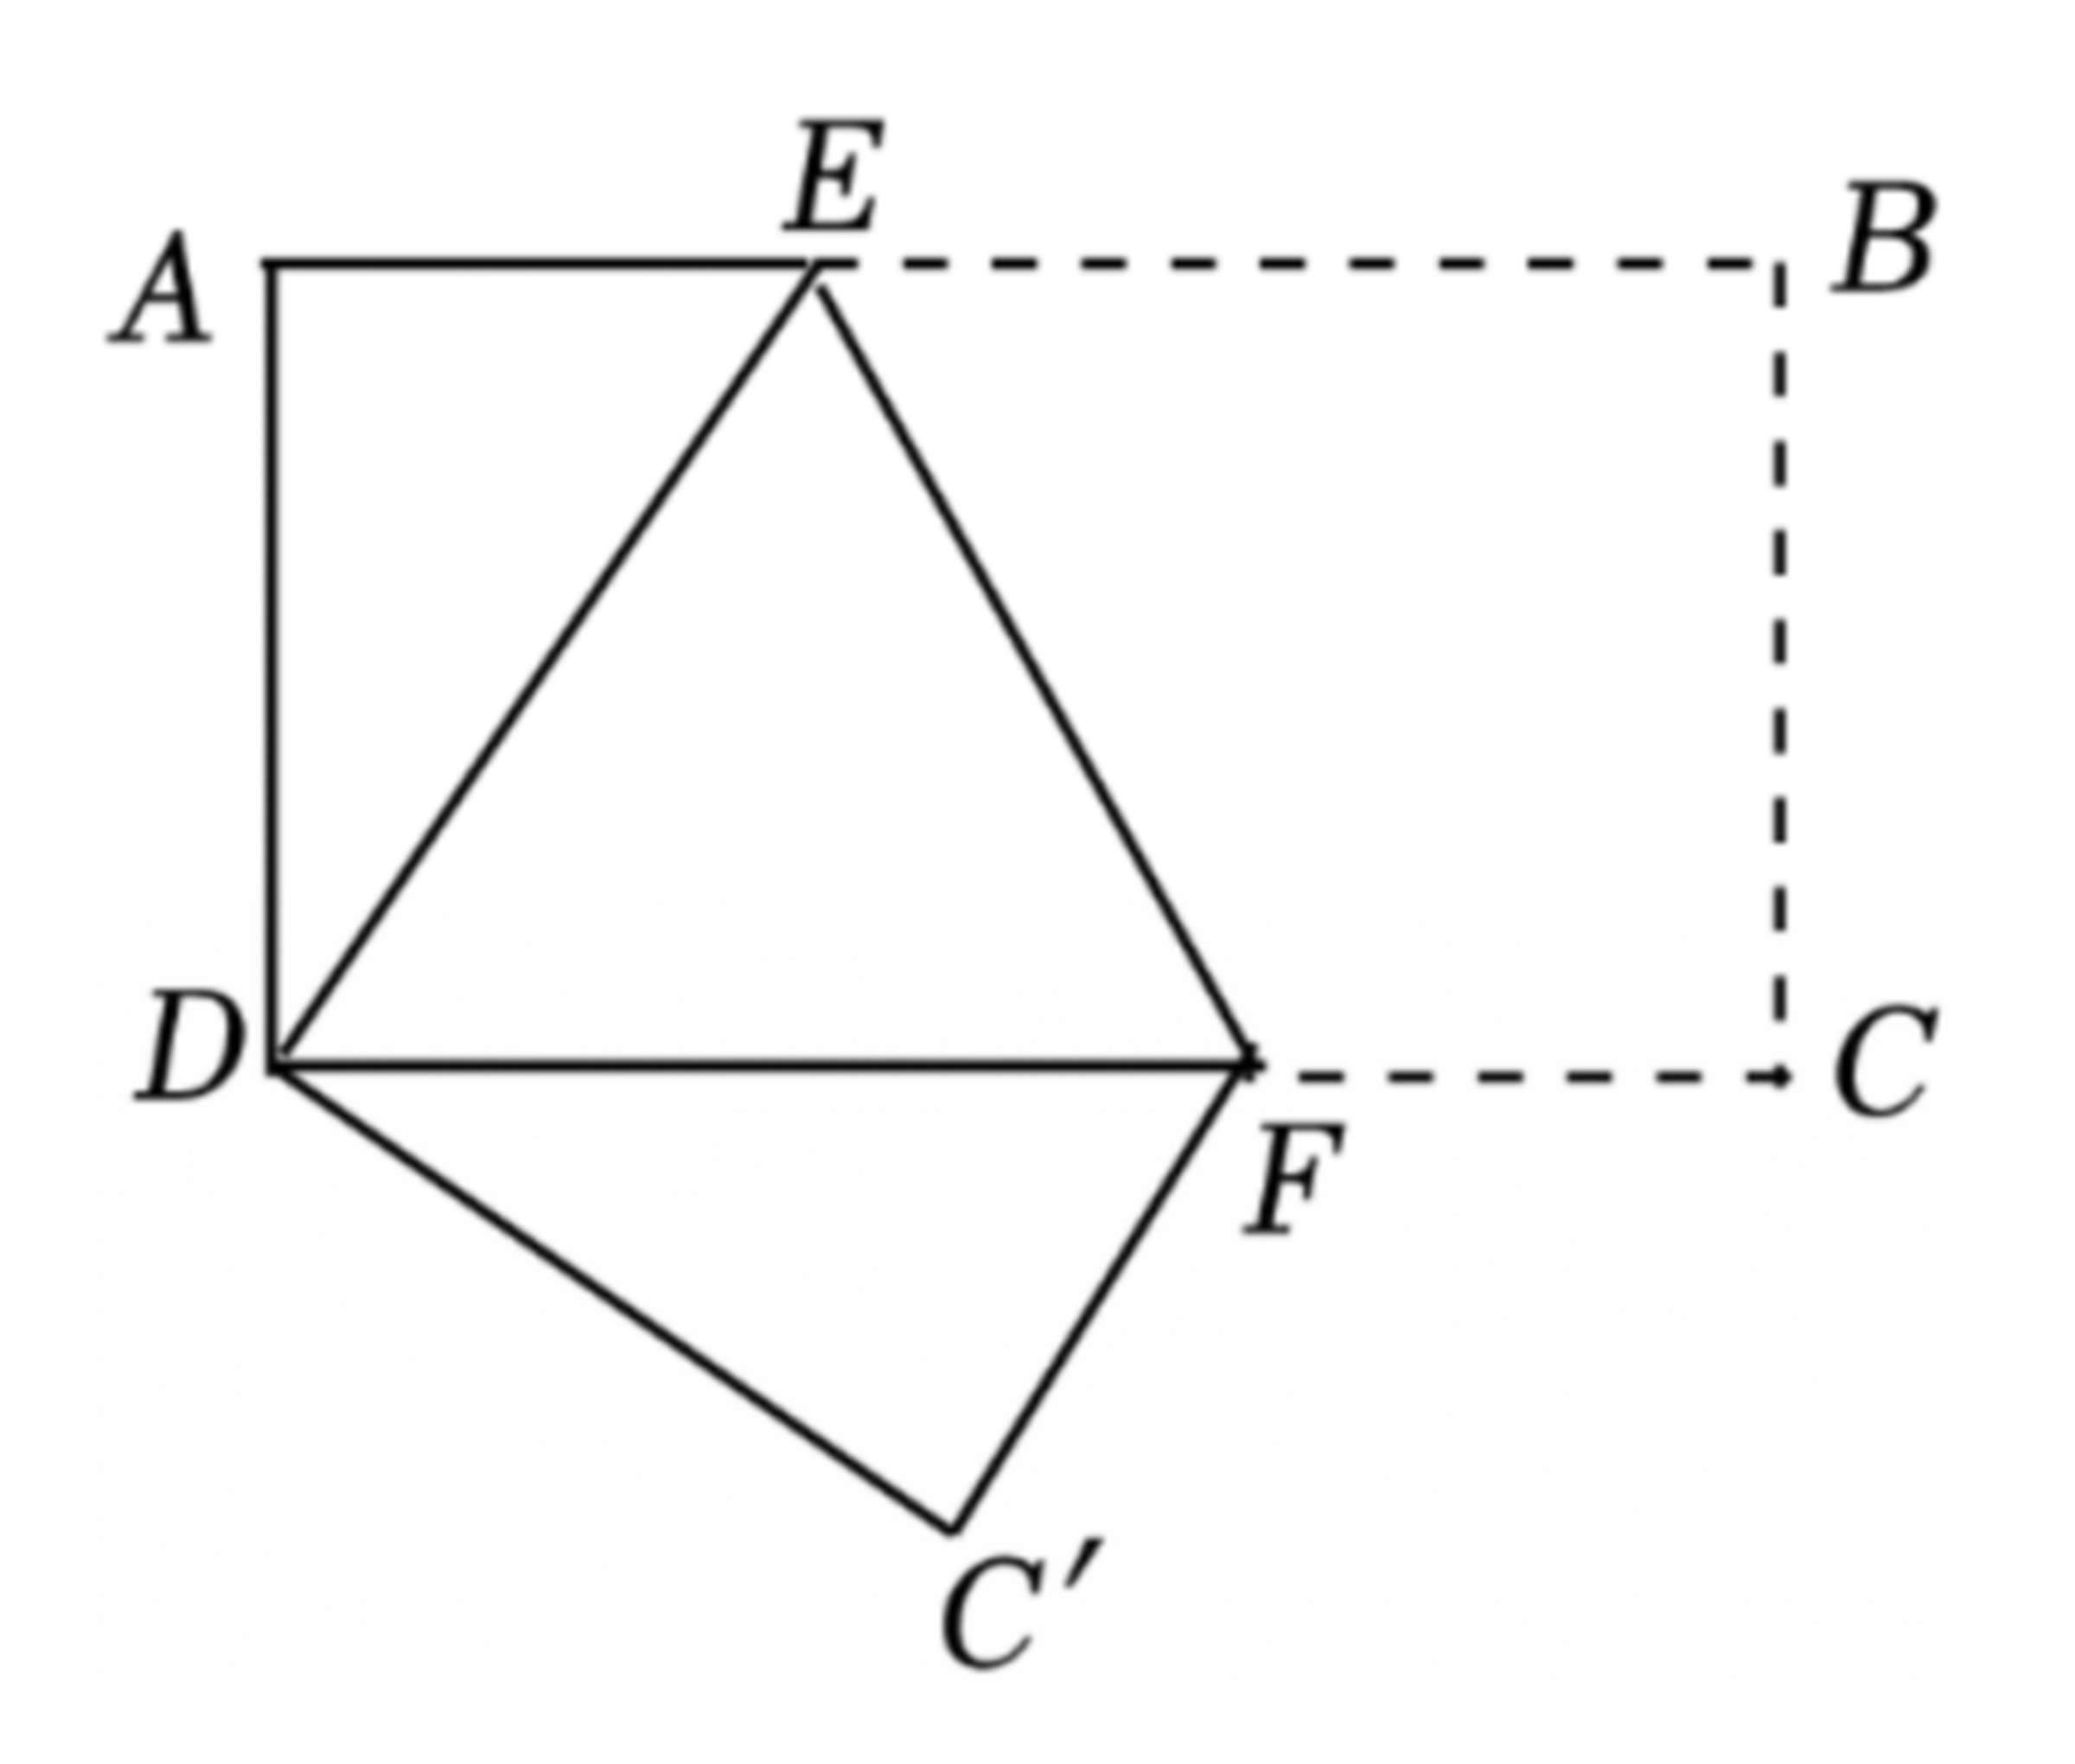
\includegraphics[width=0.40\textwidth]{figures/gao149_q11.png}
\end{center}

\ifanswer
\solbegin
\step{因为矩形 $ABCD(AB>AD)$ 的周长为 12，}
\step{在 $AB$ 和 $CD$ 边上分别取点 $E$ 和 $F$，将四边形 $BCFE$ 沿 $EF$ 折叠，}
\step{使点 $B$ 与点 $D$ 重合，此时点 $C$ 的对应点为 $C'$，}
\step{所以设 $AD=a$，$AB=b$，则 $2(a+b)=12$，}
\step{所以 $a+b=6$，且 $AB>AD$，所以 $b>a>0$，}
\step{设 $DF=x$，则 $C'F=b-x$，在 $Rt\triangle DC'F$ 中，$DC'=BC=a$，}% 几何三角形符号原卷印扁等边细线三角 $\triangle$，照录（放大 02 页确认）；$Rt$ 照录
\step{所以 $a^2+(b-x)^2=x^2$，解得 $x=\dfrac{a^2+b^2}{2b}$，}
\step{因此 $\triangle C'DF$ 的面积 $S=\dfrac{1}{2}\cdot DC'\cdot C'F=\dfrac{1}{2}\cdot a\cdot(b-x)$，}
\step{又 $b-x=b-\dfrac{(6-b)^2+b^2}{2b}=\dfrac{6(b-3)}{b}$，}
\step{所以 $S=\dfrac{1}{2}\cdot a\cdot\dfrac{6(b-3)}{b}=\dfrac{1}{2}\cdot(6-b)\cdot\dfrac{6(b-3)}{b}=\dfrac{3(6-b)(b-3)}{b}$}
\step{$=3\cdot\left(-b-\dfrac{18}{b}+9\right)$，又 $b+\dfrac{18}{b}\geqslant2\sqrt{b\cdot\dfrac{18}{b}}=6\sqrt{2}$，}
\step{当且仅当 $b=\dfrac{18}{b}$ 即 $b=3\sqrt{2}$ 时取等号，此时满足 $b>a$，}
\step{所以 $S\leqslant3\cdot(-6\sqrt{2}+9)=27-18\sqrt{2}$，故 $\triangle C'DF$ 面积的最大值为 $27-18\sqrt{2}$.}
\solend
\fi

% === Q12 === 解析内 3 幅三次函数曲线坐标图（仅答案版出）；解析 15 行（8 行 03 页＋7 行 04 页）
\item 已知 $m>0$，若存在 $t\in\R$，使得对任意 $x\in[0,m]$，不等式 $[(x-1)^2-t](x-t)\leqslant0$ 恒成立，则 $m$ 的最大值是\blankline[4.4em].

\ifanswer
\solbegin
\step{当 $t\leqslant0$ 时，$(x-1)^2-t\geqslant0$ 恒成立，}
\step{不等式 $[(x-1)^2-t](x-t)\leqslant0$ 的解集为 $x\leqslant t$，与 $x\in[0,m]$ 矛盾；}
\step{当 $t>0$ 时，不等式 $[(x-1)^2-t](x-t)\leqslant0\Leftrightarrow(x-1-\sqrt t)(x-1+\sqrt t)(x-t)\leqslant0$，}
\step{若 $t<1-\sqrt t$，即 $t\in\left(0,\dfrac{3-\sqrt5}{2}\right)$，}
\begin{center}
% 情形一 $t<1-\sqrt t$ 曲线图取 03 页右侧，去粉色水印、去色、4× LANCZOS 放大；仅答案版出
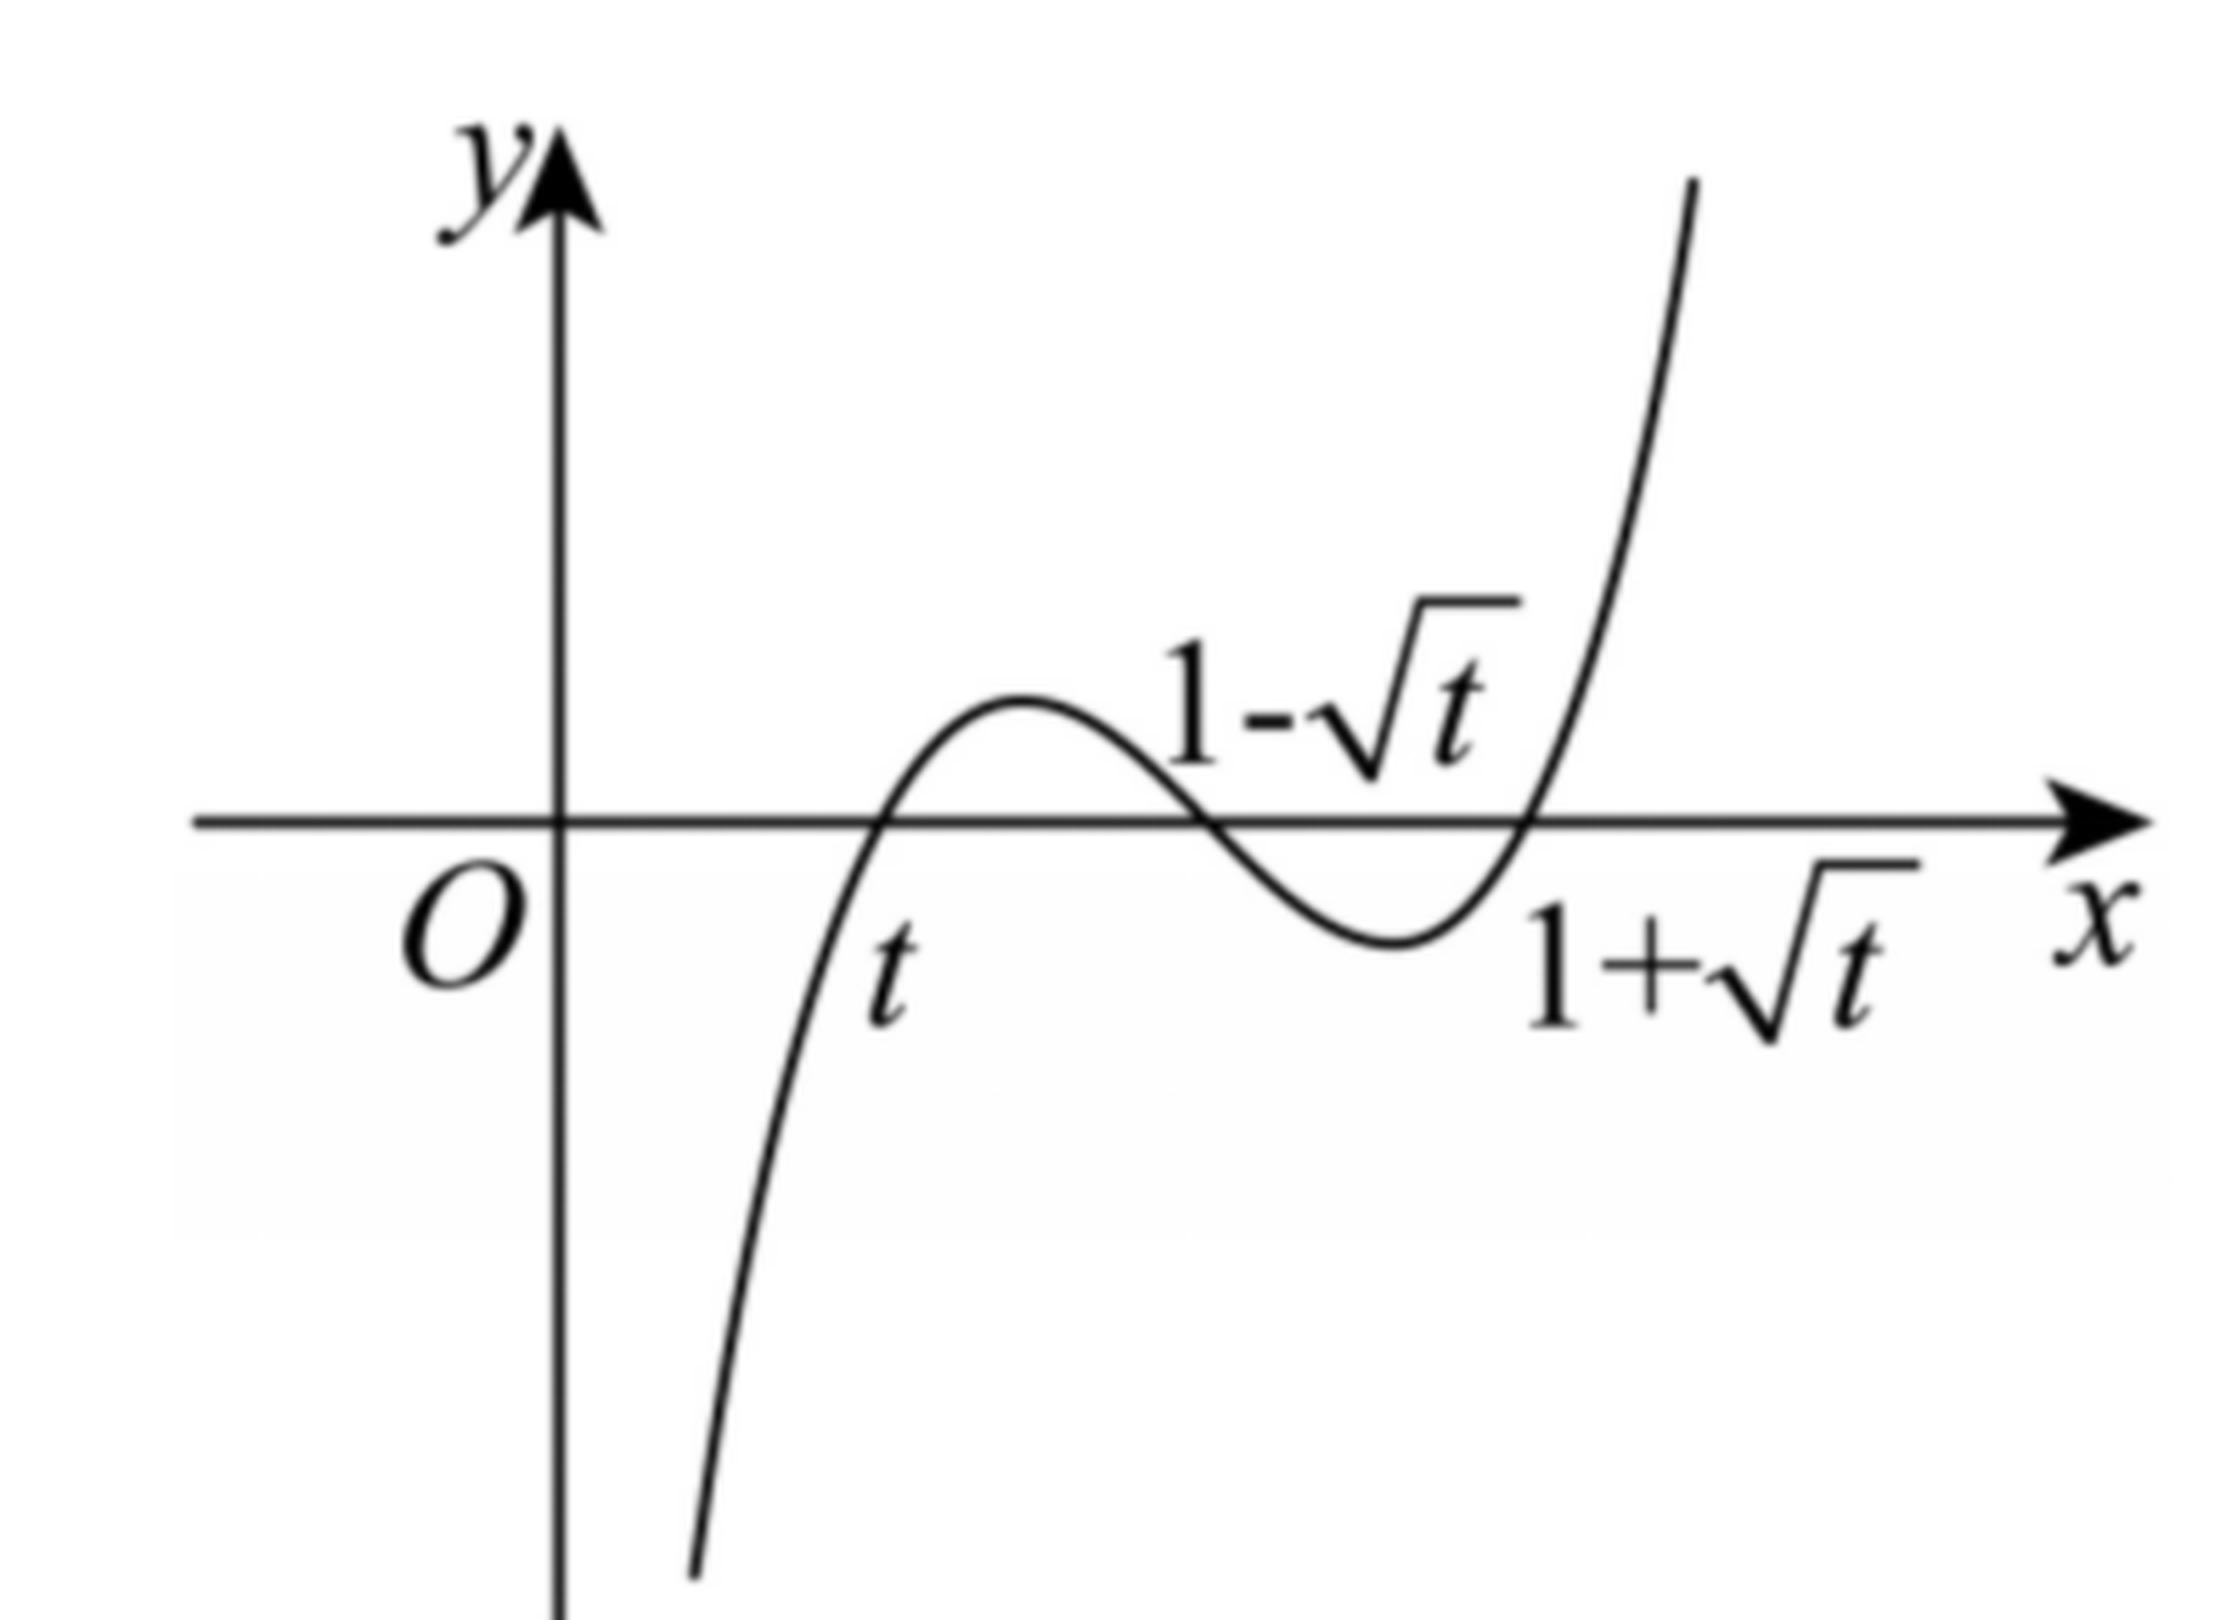
\includegraphics[width=0.40\textwidth]{figures/gao149_q12_a.png}
\end{center}
\step{则原不等式的解集为 $(-\infty,t]\cup[1-\sqrt t,1+\sqrt t]$，}
\step{当 $0<m\leqslant t$ 时，原不等式恒成立，因此}
\step{$m\in\left(0,\dfrac{3-\sqrt5}{2}\right)$；}
\step{若 $t=1-\sqrt t$，即 $t=\dfrac{3-\sqrt5}{2}$，则原不等式的解集为 $(-\infty,1+\sqrt t]$，}
\begin{center}
% 情形二 $t=1-\sqrt t$ 曲线图取 03 页右侧，去粉色水印、去色、4× LANCZOS 放大；仅答案版出
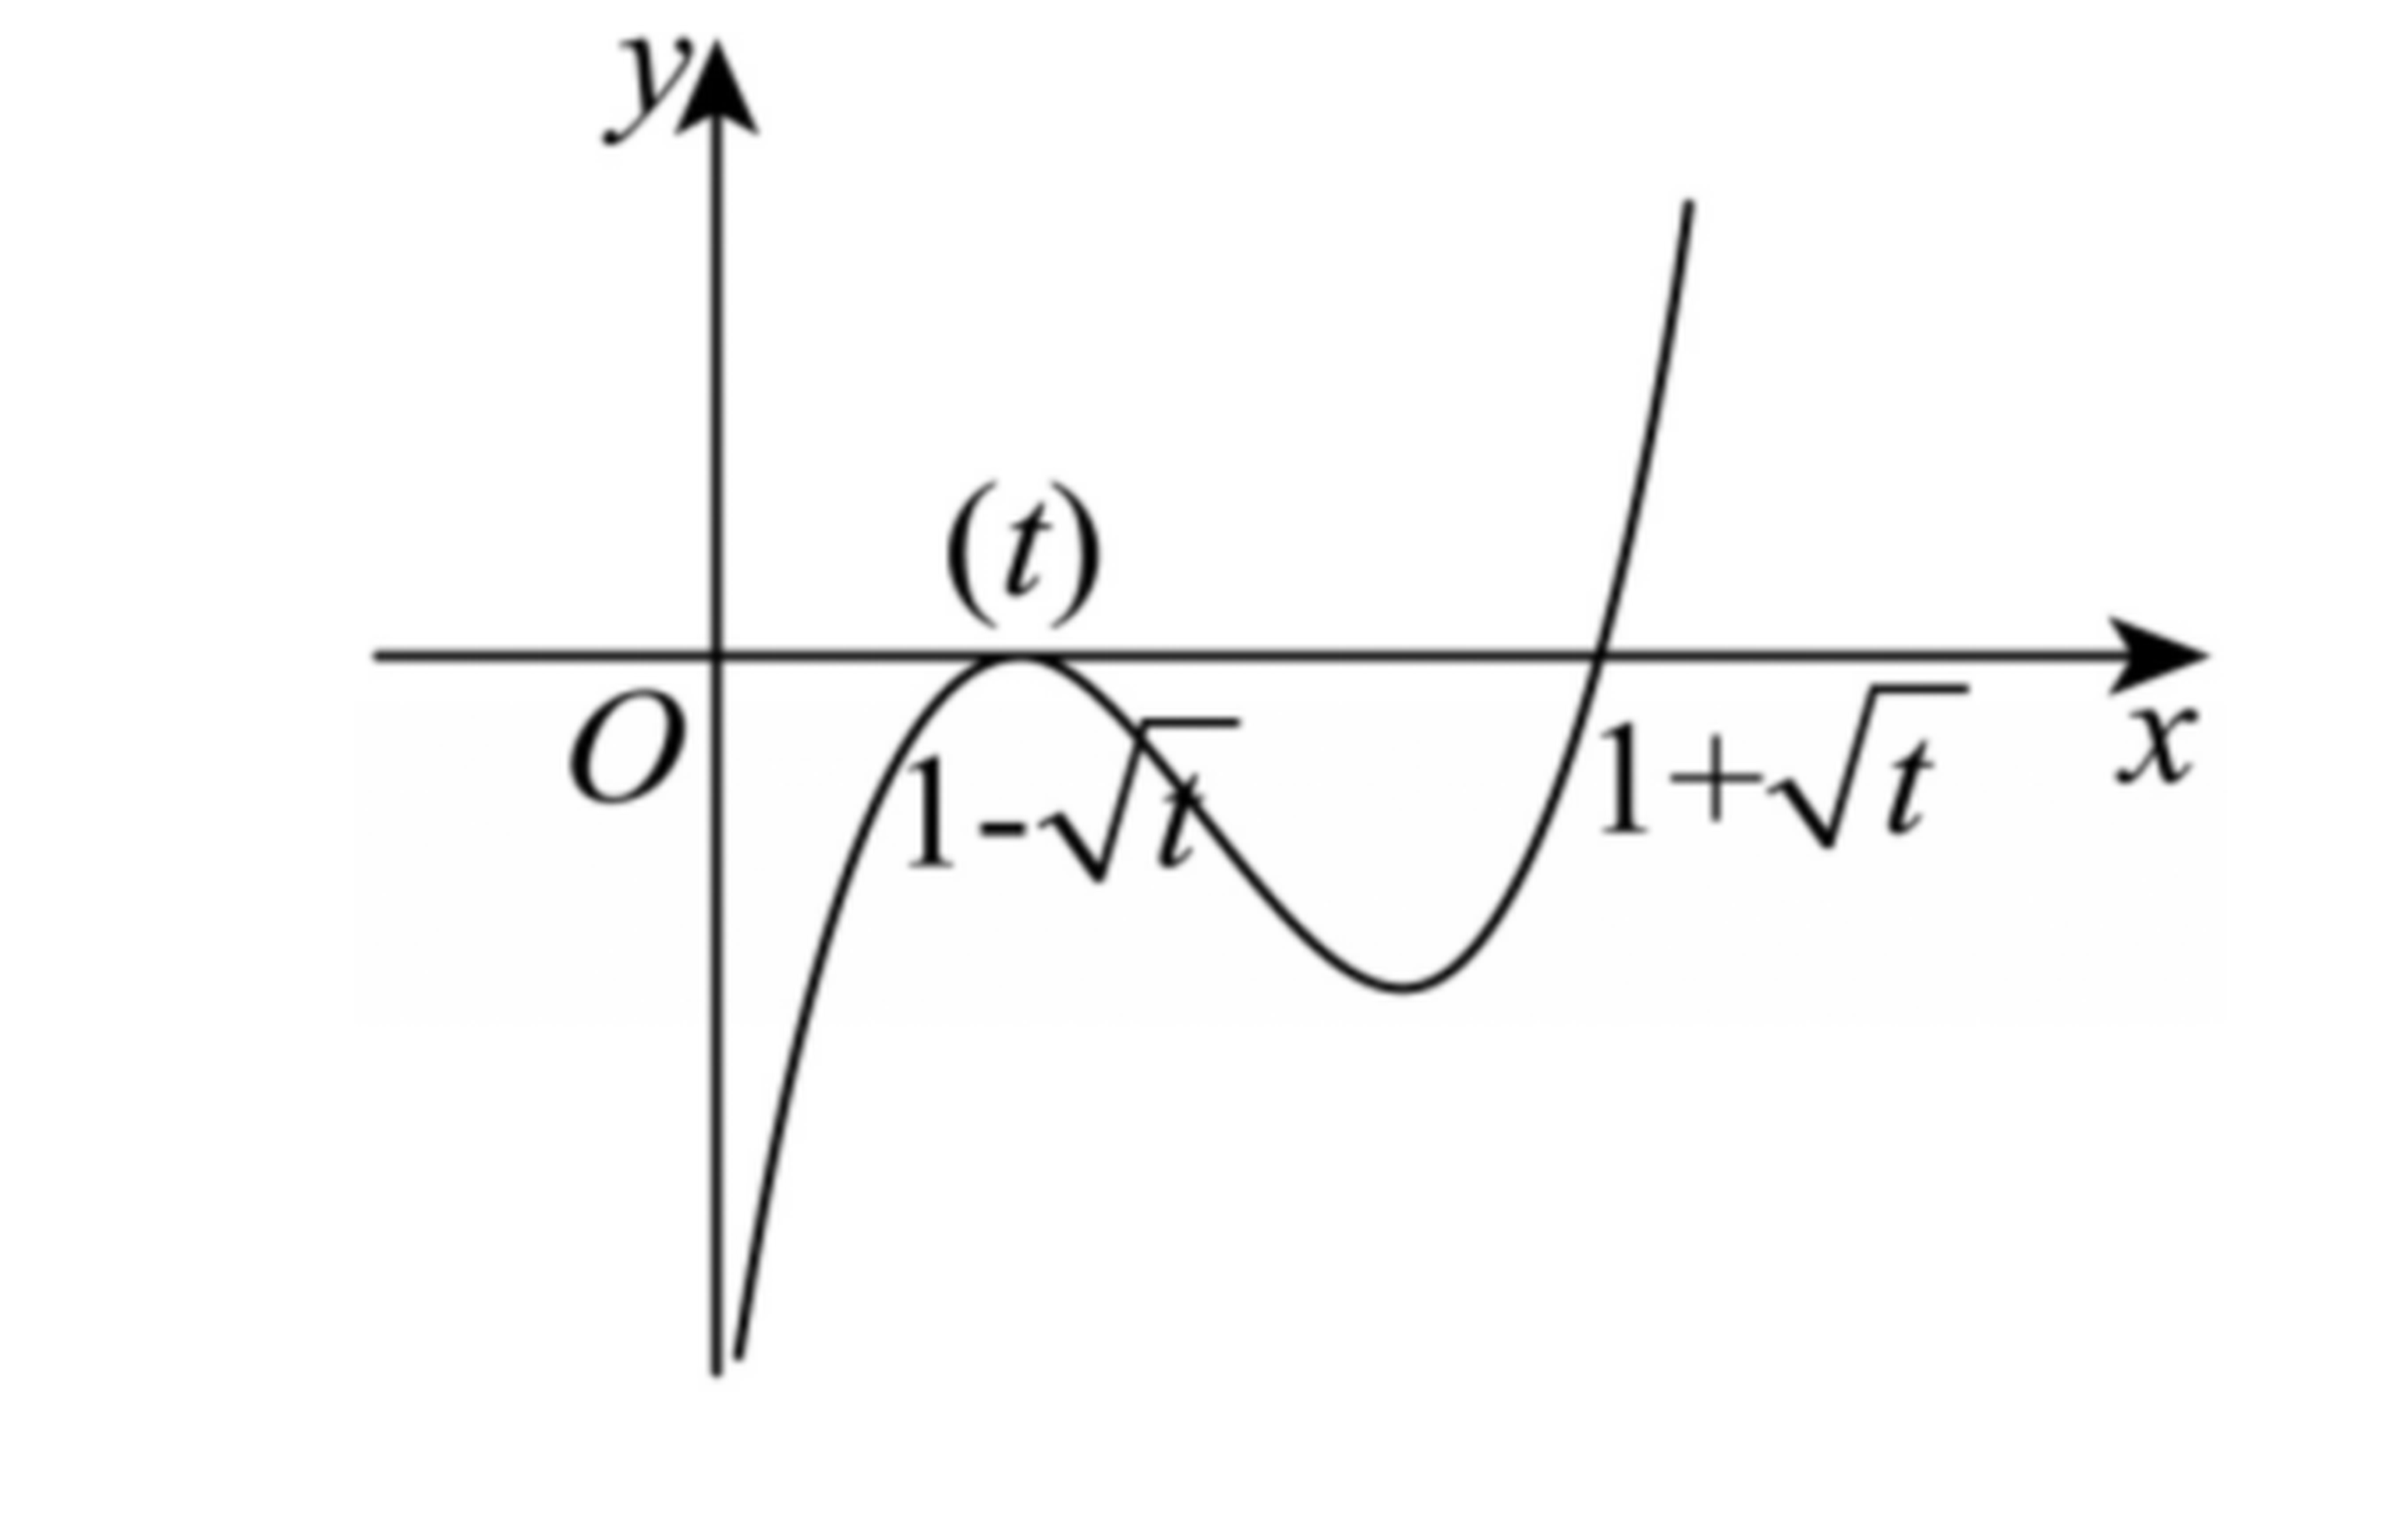
\includegraphics[width=0.40\textwidth]{figures/gao149_q12_b.png}
\end{center}
\step{当 $0<m\leqslant1+\sqrt t$ 时，原不等式恒成立，因此 $m\in\left(0,\dfrac{\sqrt5+1}{2}\right]$；}
\step{若 $1+\sqrt t>t>1-\sqrt t$，即 $t\in\left(\dfrac{3-\sqrt5}{2},\dfrac{3+\sqrt5}{2}\right)$，}
\begin{center}
% 情形三 $1+\sqrt t>t>1-\sqrt t$ 曲线图取 04 页右侧，去粉色水印、去色、4× LANCZOS 放大；仅答案版出
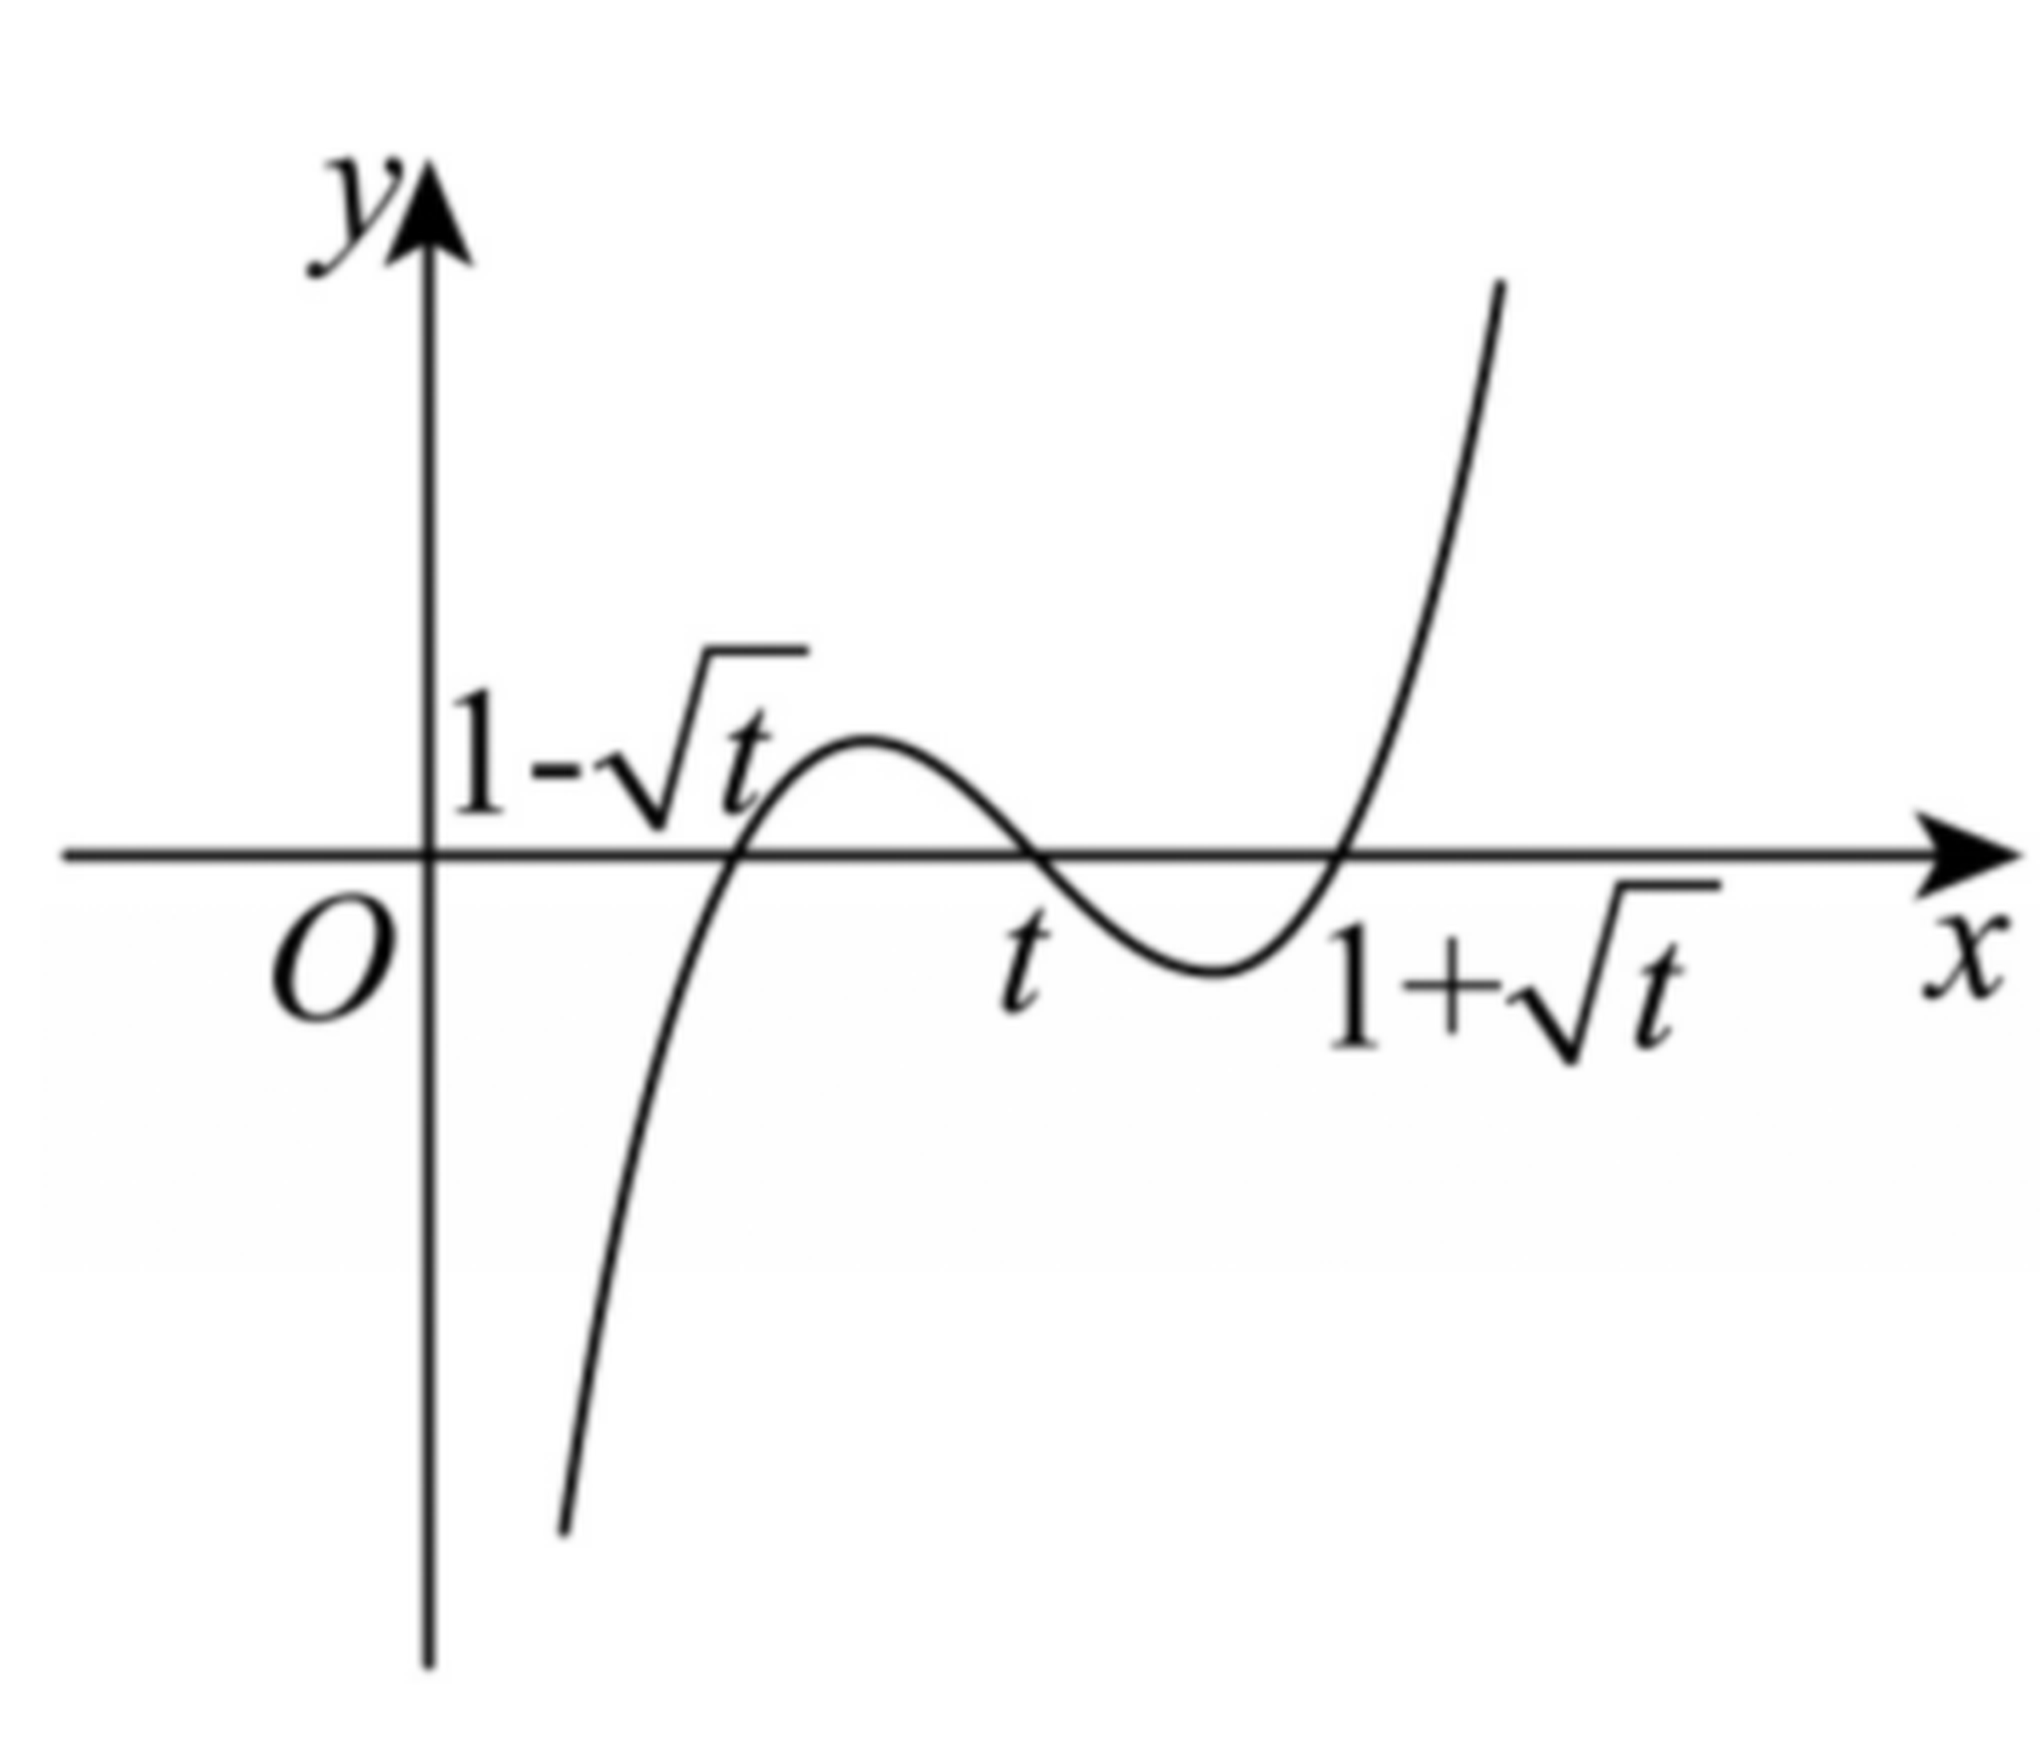
\includegraphics[width=0.40\textwidth]{figures/gao149_q12_c.png}
\end{center}
\step{则原不等式的解集为 $(-\infty,1-\sqrt t]\cup[t,1+\sqrt t]$，}
\step{当 $\begin{cases}1-\sqrt t>0\\1-\sqrt t\geqslant m\end{cases}$ 时，原不等式恒成立，此时 $t\in\left(\dfrac{3-\sqrt5}{2},1\right)$，$m\in\left(0,\dfrac{3-\sqrt5}{2}\right)$；}
\step{若 $t\geqslant1+\sqrt t$，即 $t\geqslant\dfrac{3+\sqrt5}{2}$，则取 $x=0$，$(t-1)t>0$，}
\step{原不等式不恒成立，不符合题意，}
\step{因此实数 $m$ 的取值范围是 $\left(0,\dfrac{\sqrt5+1}{2}\right]$，$m$ 的最大值是 $\dfrac{\sqrt5+1}{2}$.}
\solend
\fi

\end{enumerate}

\bigsec{二、选择题}

\begin{enumerate}
\setcounter{enumi}{12}

% === Q13 ===：答案"C"直接印在题干括号内、无【答案】/【解析】段，按 高一84 Q13／高一148 Q13 成例括号留空、另提 \ans{$C$}；四选项两行两列照原卷分行
\item 设 $ab>0$，则 $a>b$ 是 $\dfrac{1}{a}<\dfrac{1}{b}$ 的\mbox{（\quad）}

\keepwithprev
A. 充分不必要条件\qquad\qquad B. 必要不充分条件

C. 充要条件\qquad\qquad D. 既不充分又不必要条件

\ifanswer
\ans{$C$}
\fi

% === Q14 ===：$A\subset B$ 单线照录；四选项补集照原卷上划线 \overline{A}／\overline{B}；解析 1 行（由韦恩图得 B 对）
\item 已知集合 $A$、$B$ 非空，且 $A\subset B$，则下列式子中一定是空集的为\mbox{（\quad）}

\keepwithprev
A. $\overline{A}\cap B$\qquad B. $A\cap\overline{B}$\qquad C. $\overline{A}\cap\overline{B}$\qquad D. $\overline{A}\cup\overline{B}$

\ifanswer
\solbegin
\step{由韦恩图得 $B$ 对. 故选 $B$.}
\solend
\fi

% === Q15 ===："天文数字"弯引号照录；解析 2 行（首行在 04 页末、末行续 05 页顶）
\item 历史上数学计算方面的三大发明是阿拉伯数字、十进制和对数，其中对数的发明，大大缩短了计算时间，为人类研究科学和了解自然起了重大作用，对数运算对估算“天文数字”具有独特的优势. $2.5^{1000}$ 的估算值约为\mbox{（\quad）}

\keepwithprev
A. $10^{365}$\qquad B. $10^{379}$\qquad C. $10^{389}$\qquad D. $10^{398}$

\ifanswer
\solbegin
\step{$\lg 2.5^{1000}=1000\lg 2.5=1000(1-2\lg 2)\approx1000\times(1-0.602)=398$，}
\step{所以 $2.5^{1000}\approx10^{398}$. 故选 $D$.}
\solend
\fi

% === Q16 ===："完美集"新定义、圈数字①②文本模式；题干"若对任意 $x$，$y\in A$"用全角逗号、解析用顿号"$x$、$y\in A$"，两处照录不统一；解析 9 行
\item 设全集 $U=\R$，集合 $A$ 是一个非空数集，若对任意 $x$，$y\in A$，都有 $x+y\in A$、$xy\in A$，则称集合 $A$ 为一个“完美集”，给出以下命题：

①若 $A_1$、$A_2$ 都是“完美集”，且 $A_1\cap A_2\ne\varnothing$，则 $A_1\cap A_2$ 也是“完美集”；

②若 $A_1$、$A_2$ 都是“完美集”，则 $A_1\cup A_2$ 也是“完美集”.

下列说法正确的是\mbox{（\quad）}

\keepwithprev
A. ①②都是真命题\qquad\qquad B. ①是真命题，②是假命题

C. ①是假命题，②是真命题\qquad\qquad D. ①②都是假命题

\ifanswer
\solbegin
\step{由题意，全集 $U=\R$，集合 $A$ 是一个非空数集，}
\step{若对任意 $x$、$y\in A$，都有 $x+y\in A$、$xy\in A$，则称集合 $A$ 为一个“完美集”，}
\step{对于①，取 $x$、$y\in A_1\cap A_2$，则 $x\in A_1$，$x\in A_2$，$y\in A_1$，$y\in A_2$，}
\step{又 $A_1$、$A_2$ 是“完美集”，所以 $x+y\in A_1$，$xy\in A_1$，$x+y\in A_2$，$xy\in A_2$，}
\step{所以 $x+y\in A_1\cap A_2$，$xy\in A_1\cap A_2$，所以 $A_1\cap A_2$ 是“完美集”，故①正确；}
\step{对于②，取“完美集” $A_1=\{x\mid x=2k,k\in\Z\}$，$A_2=\{x\mid x=3k,k\in\Z\}$，}
\step{则 $2\in A_1$，$3\in A_2$，但 $2+3\notin A_1\cup A_2$，}
\step{即此时 $A_1\cup A_2$ 不是“完美集”，故②错误.}
\step{故选 $B$.}
\solend
\fi
\end{enumerate}

\bigsec{三、解答题}

\begin{enumerate}
\setcounter{enumi}{16}

% === Q17 ===："图像"（有亻）照录（Q17 题干与解析共 2 处）；绝对值 \lvert…\rvert；解析 7 行
\item 已知 $m\in\R$，$f(x)=(m^2-m-5)x^m$. 若 $y=f(x)$ 是幂函数，且其图像不经过原点.

(1) 求实数 $m$ 的值；

(2) 若 $f(a)=f(b)$ 且 $a\ne b$，求 $\lvert a+2\rvert+\lvert b-1\rvert$ 的最小值，并指出取到最小值时 $a$ 的取值范围.

\ifanswer
\solbegin
\step{(1) $f(x)=(m^2-m-5)x^m$ 是幂函数，得 $m^2-m-5=1$，即 $m^2-m-6=0$，}
\step{解得 $m=-2$ 或 $m=3$，又函数图像不经过原点，所以 $m=-2$($3$ 舍)；}
\step{(2) 由 (1) 得 $f(x)=x^{-2}=\dfrac{1}{x^2}$ 为偶函数，}
\step{$x<0$ 时，函数 $f(x)$ 严格增，$x>0$ 时，函数 $f(x)$ 严格减，}
\step{又 $f(a)=f(b)$ 且 $a\ne b$，所以 $a=-b$，且 $a\ne0$，$b\ne0$，}
\step{则 $\lvert a+2\rvert+\lvert b-1\rvert=\lvert a+2\rvert+\lvert-a-1\rvert=\lvert a+2\rvert+\lvert a+1\rvert$，}
\step{则 $\lvert a+2\rvert+\lvert b-1\rvert$ 的最小值为 $1$，取到最小值时 $a$ 的取值范围是 $[-2,-1]$.}
\solend
\fi

% === Q18 ===：判别式两形混用——(1) cases 块印高 \Delta、(2) 独立行印扁 \triangle，逐处照录不统一；解析 8 行
\item 已知命题 $p$：方程 $x^2+4x+m-1=0$ 有两个不等的负根；命题 $q$：方程 $4x^2+4x+m-2=0$ 无实根.

(1) 若 $p$ 为真命题，求 $m$ 的取值范围；

(2) 若 $p$、$q$ 两命题一真一假，求 $m$ 的取值范围.

\ifanswer
\solbegin
\step{(1) 若 $p$ 为真命题，即方程 $x^2+4x+m-1=0$ 有两个不等的负根；}
\step{必有 $\begin{cases}\Delta=16-4(m-1)>0\\m-1>0\end{cases}$，解得 $1<m<5$，即 $m$ 的取值范围为 $(1,5)$；}
\step{(2) 命题 $q$：方程 $4x^2+4x+m-2=0$ 无实根，}
\step{则有 $\triangle=16-16(m-2)<0$，解得 $m>3$，}
\step{若 $p$ 和 $q$ 有且只有一个为真命题，}
\step{若 $p$ 真 $q$ 假，必有 $\begin{cases}1<m<5\\m\leqslant3\end{cases}$，则有 $1<m\leqslant3$，}
\step{若 $p$ 假 $q$ 真，必有 $\begin{cases}m\leqslant1\text{ 或 }m\geqslant5\\m>3\end{cases}$，则有 $m\geqslant5$，}
\step{综上，$1<m\leqslant3$ 或 $m\geqslant5$.}
\solend
\fi

% === Q19 ===：$A\subseteq B$ 带下划线照录；解析 7 行（(2) 两组 cases 并排）
\item 已知 $m\in\R$，集合 $A=\left\{x\mid y=\sqrt{3-x}-\dfrac{1}{\sqrt{x-1}}\right\}$，集合 $B=\{x\mid 2m\leqslant x\leqslant1-m\}$.

(1) 若 $A\cup B=B$，求实数 $m$ 的取值范围；

(2) 若 $A\cap B=\varnothing$，求实数 $m$ 的取值范围.

\ifanswer
\solbegin
\step{(1) 函数 $y=\sqrt{3-x}-\dfrac{1}{\sqrt{x-1}}$，则 $\begin{cases}3-x\geqslant0\\x-1>0\end{cases}$，解得 $1<x\leqslant3$，}
\step{所以 $A=\{x\mid1<x\leqslant3\}$，}
\step{因为 $A\cup B=B$，所以 $A\subseteq B$，则 $\begin{cases}2m\leqslant1\\1-m\geqslant3\end{cases}$，解得 $m\leqslant-2$，}
\step{综上，实数 $m$ 的取值范围为 $(-\infty,-2]$；}
\step{(2) 当 $B=\varnothing$ 时，则 $2m>1-m$，解得 $m>\dfrac{1}{3}$，}
\step{当 $B\ne\varnothing$ 时，则 $\begin{cases}2m\leqslant1-m\\2m>3\end{cases}$ 或 $\begin{cases}2m\leqslant1-m\\1-m\leqslant1\end{cases}$，解得 $m\in\varnothing$ 或 $0\leqslant m\leqslant\dfrac{1}{3}$，}
\step{综上，实数 $m$ 的取值范围为 $[0,+\infty)$.}
\solend
\fi

% === Q20 ===：n 阶基本不等式推广；(3) 解析含 \overbrace{…}^{k} 上括号；(2) 解析"x=x=x=3(1-x)"三连等系原卷笔误、照录加注（见 ⑤）；解析 14 行
\item 教材中的基本不等式可以推广到 $n$ 阶：$n$ 个正数的算术平均数不小于它们的几何平均数，即对于任意的正数 $a_1$、$a_2$、$\cdots$、$a_n$，有 $\dfrac{a_1+a_2+\cdots+a_n}{n}\geqslant\sqrt[n]{a_1\cdot a_2\cdots a_n}$（$n\in\N$ 且 $n\geqslant2$），且等号当且仅当 $a_1=a_2=\cdots=a_n$ 时成立. 利用此结论解决下列问题：

(1) 若 $x$、$y$、$z>0$，求 $\dfrac{y}{x}+\dfrac{2z}{y}+\dfrac{4x}{z}$ 的最小值；

(2) 已知 $0<x<1$，求 $x^3(1-x)$ 的最大值，并求取得最大值时的 $x$ 的值；

(3) 对任意的正整数 $k$，判断 $\left(1+\dfrac{1}{k}\right)^k$ 与 $\left(1+\dfrac{1}{k+1}\right)^{k+1}$ 的大小关系，并证明.

\ifanswer
\solbegin
\step{(1) 因为 $x$、$y$、$z>0$，有 $\dfrac{y}{x}>0$，$\dfrac{2z}{y}>0$，$\dfrac{4x}{z}>0$}
\step{所以 $\dfrac{y}{x}+\dfrac{2z}{y}+\dfrac{4x}{z}\geqslant3\sqrt[3]{\dfrac{y}{x}\cdot\dfrac{2z}{y}\cdot\dfrac{4x}{z}}=3\sqrt[3]{8}=6$，}
\step{当且仅当 $\dfrac{y}{x}=\dfrac{2z}{y}=\dfrac{4x}{z}$ 时取等号，故 $\dfrac{y}{x}+\dfrac{2z}{y}+\dfrac{4x}{z}$ 的最小值为 $6$.}
\step{(2) 因为 $0<x<1$，所以 $1-x>0$，}
\step{$x^3(1-x)=\dfrac{1}{3}[x\cdot x\cdot x\cdot3(1-x)]\leqslant\dfrac{1}{3}\left[\dfrac{x+x+x+3(1-x)}{4}\right]^4=\dfrac{1}{3}\times\left(\dfrac{3}{4}\right)^4$}
\step{$=\dfrac{27}{256}$，当且仅当 $x=x=x=3(1-x)$，即 $x=3(1-x)$，$x=\dfrac{3}{4}$ 取等号，}% 原卷"x=x=x=3(1-x)"三连等，疑为四因子相等之误排，放大 08 页确认，照录未改（见 ⑤）
\step{所以 $0<x<1$ 时，$x^3(1-x)$ 的最大值是 $\dfrac{27}{256}$，取最大值时 $x=\dfrac{3}{4}$.}
\step{(3) 对任意 $k\in\N^*$，$\left(1+\dfrac{1}{k}\right)^k<\left(1+\dfrac{1}{k+1}\right)^{k+1}$.}
\step{证明：$\left(1+\dfrac{1}{k}\right)^k=\overbrace{\left(1+\dfrac{1}{k}\right)\cdot\left(1+\dfrac{1}{k}\right)\cdots\left(1+\dfrac{1}{k}\right)}^{k}\times1$}
\step{$\leqslant\left(\dfrac{\overbrace{\left(1+\dfrac{1}{k}\right)+\left(1+\dfrac{1}{k}\right)+\cdots+\left(1+\dfrac{1}{k}\right)}^{k}+1}{k+1}\right)^{k+1}$}
\step{$=\left(\dfrac{\overbrace{(1+1+\cdots+1)}^{k}+\overbrace{\left(\dfrac{1}{k}+\dfrac{1}{k}+\cdots+\dfrac{1}{k}\right)}^{k}+1}{k+1}\right)^{k+1}=\left(\dfrac{k+1+1}{k+1}\right)^{k+1}=\left(1+\dfrac{1}{k+1}\right)^{k+1}$，}
\step{当且仅当 $1+\dfrac{1}{k}=1$ 时取等号，}
\step{但是任意 $k\in\N^*$ 时 $1+\dfrac{1}{k}>1$，所以等号不成立，}
\step{故任意 $k\in\N^*$ 时，$\left(1+\dfrac{1}{k}\right)^k<\left(1+\dfrac{1}{k+1}\right)^{k+1}$.}
\solend
\fi

% === Q21 ===："减 k 集"新定义（引号内 k／数字两侧空格照录）；解析 26 行（续 10 页），含 ⑤ 三处原卷笔误照录
\item 定义：对于给定的整数 $k$，若非空集合 $A$ 满足如下 3 个条件：

① $A$ 是正整数集的子集；② $A\ne\{1\}$；

③对任意正整数 $x,y$，若 $x+y\in A$，则 $xy-k\in A$；则称集合 $A$ 为“减 $k$ 集”.

(1) 判断集合 $A=\{1,2\}$ 是否为“减 $0$ 集”？是否为“减 $1$ 集”？（无需说明理由）

(2) 证明：不存在“减 $2$ 集”；

(3) 是否存在“减 $1$ 集”？如果存在，求出所有“减 $1$ 集”；如果不存在，说明理由.

\ifanswer
\solbegin
\step{(1) 因为 $P\subseteq\N^*$，$P\ne\{1\}$，$1+1=2\in P$，$1\times1-0\in P$，}
\step{所以集合 $P=\{1,2\}$ 是“减 $0$ 集”；}
\step{因为 $P\subseteq\N^*$，$P\ne\{1\}$，$1+1=2\in P$，$1\times1-1\notin P$，}
\step{所以集合 $P=\{1,2\}$ 是“减 $1$ 集”；}% 按条件③应为"不是"，原卷径印"是"，放大 09 页确认，照录未改（见 ⑤）
\step{(2) 假设存在集合 $A$ 是“减 $2$ 集”，若 $x+y\in A$，则 $xy-2\in A$，}
\step{①当 $x+y=xy-2$ 时，有 $(x-1)(y-1)=3$，}
\step{则 $x$、$y$ 一个为 $2$，一个为 $4$，所以集合 $A$ 有元素 $6$，}
\step{但 $3+3\in A$，$3\times3-2\notin A$，与 $A$ 是“减 $2$ 集”矛盾；}
\step{②当 $x+y\ne xy-2$ 时，则 $x+y=xy-1$ 或 $x+y=xy-m$($m>2$)，}
\step{若 $x+y=xy-1$，$m=1$ 时，$M$ 为除 $1$ 以外的最小元素，}% 原卷"m=1"上文未显式定义，疑笔误，放大 09 页确认，照录未改（见 ⑤）
\step{则 $x=M-1$，$y=1$ 时，$xy-2=M-3$ 小于 $M$，}
\step{要符合题意，必须 $M=4$，}
\step{此时取 $x-2$，$y=2$，$xy-2=2$ 不属于 $A$，故不符合题意，}% 原卷"取 x−2"疑为"取 x=2"误排，放大 09 页确认，照录未改（见 ⑤）
\step{当 $m>2$ 时，$(x-1)(y-1)=m+1$，同样得出矛盾，}
\step{综上，不存在 $A$ 是“减 $2$ 集”.}
\step{(3) 存在“减 $1$ 集” $A$，则 $A\ne\{1\}$，}
\step{①假设 $1\in A$，则 $A$ 中除了元素 $1$ 以外，必然还含有其它元素，}
\step{假设 $2\in A$，$1+1\in A$，而 $1\times1-1\notin A$，所以 $2\notin A$，}
\step{假设 $3\in A$，$1+2\in A$，而 $1\times2-1\in A$，所以 $3\in A$，}
\step{所以 $A=\{1,3\}$，}
\step{假设 $4\in A$，$1+3\in A$，而 $1\times3-1\notin A$，所以 $4\notin A$，}
\step{假设 $5\in A$，$1+4\in A$，$1\times4-1\in A$，$2+3=5$，$2\times3-1\in A$，所以 $5\in A$，}
\step{所以 $A=\{1,3,5\}$，}
\step{以此类推，得 $A=\{1,3,5,\cdots,2n-1,\cdots\}$，($n\in\N^*$)，}
\step{所以所有的“减 $1$ 集”有 $\{1,3\}$，$\{1,3,5\}$，$\{1,3,5,7\}$，$\cdots$，$\{1,3,5,\cdots,2n-1,\cdots\}$，}
\step{$(n\in\N^*)$.}
\solend
\fi
\end{enumerate}

\end{document}
"
% 紧凑版：xelatex "\def\iscompact{1}% 高一149_青浦高级中学上外云间_期中.tex
%   —— 高一上数学"2026-2027 年青浦高级中学上外云间高一上期中"（试卷版/答案版/紧凑版）
% 试卷版：xelatex 高一149_青浦高级中学上外云间_期中.tex
% 答案版：xelatex "\def\isanswer{1}\input{高一149_青浦高级中学上外云间_期中.tex}"
% 紧凑版：xelatex "\def\iscompact{1}\input{高一149_青浦高级中学上外云间_期中.tex}"
%
% ① 原始材料：微信公众号"魔都数学加油站"文章，连载"27学年高一149"，原文标题
% "27学年高一149——2026-2027年上海市青浦高级中学上外云间高一上期中"；
% 原文链接：https://mp.weixin.qq.com/s/T7_nyoR1k0o_5og7FkDsyw 。
% 正文为 10 张 PNG 页（01/02/03/04/10 为 2560×3620，05/06/07/08/09 为 4762×6735，
% 同一篇各页分辨率混排，逐页按各自分辨率裁图核对，别按预览比例换算裁框）。
% 体例：混合体例讲评版——19 题中 Q6 只印【答案】、无【解析】；Q13 的答案"C"
%   直接印在题干括号内、无【答案】/【解析】段；其余 17 题印【解析】（逐题核实，见 ② ②）。
% 题目、答案、解析均据原图转录；卷面粉红色水印"魔都数学加油站"及公众号页脚未录入。
% 全卷插图清单（逐页通读 10 页确认）：1 幅题目配图 + 3 幅【解析】内配图：
%   · Q11 矩形 ABCD 折叠几何图（02 页右侧：A/B/C/D/E/F/C' 与虚线 EB、BC、FC），
%     题干"如图"处，题目配图、三版都出，裁 figures/gao149_q11.png；
%   · Q12【解析】内 3 幅三次函数曲线坐标图（03 页右侧两幅 + 04 页右侧一幅：
%     x/y 轴、O、t、1-\sqrt t、1+\sqrt t 等标注，分别对应 t<1-\sqrt t、
%     t=1-\sqrt t、1+\sqrt t>t>1-\sqrt t 三种情形），解析配图、仅答案版出，
%     分别裁 figures/gao149_q12_a.png／_b.png／_c.png，放 \ifanswer 内 \step 之间
%     （高一73 第 16 题成例）；
%   其余各页逐页确认无其它题目配图、无表格；Q14 解析"由韦恩图得 B 对"仅文字推导、
%   原卷并未印韦恩图；Q9／Q18／Q19 的 cases 块与 Q20(3) 的 \overbrace 为数学块（非图）；
%   10 页下半仅水印、无正文。4 图均取自原卷截图，去粉色水印、去色、4× LANCZOS 放大。
%
% 卷首标题：原卷印作"2026-2027 年青浦高级中学上外云间高一上期中"，年份区间按全稿
% 惯例排 en dash；原卷卷面未印副标题，本稿按同期中卷（高一140／141／143／144／145／
% 146／147／148）知识模块口径补出"集合与常用逻辑用语、不等式、函数"。
%
% 题号体例（逐页核实定稿）：本卷共 19 题——一、填空题 3—12（10 题）、
% 二、选择题 13—16（4 题）、三、解答题 17—21（5 题）。
% 三节分别 \setcounter{enumi}{2}／{12}／{16}。原卷从第 3 题起、无第 1、2 题，
% 本稿保留原题号；全卷无附加题节（Q21 解析末行"（n\in N^*）."为全卷收尾）。
%
% ② 与原卷的排版差异：
%   ① 原文从第 3 题起，本稿保留原题号；共 19 题三节；
%   ② 混合体例逐题核实：Q6（反证法"假设的内容"）只印【答案】、无【解析】，
%      按 高一140 第 5 题／高一145 Q3 成例提 \ans{}、不补造解析；Q13 答案"C"直接
%      印在题干括号内、全卷无该题【答案】/【解析】段，按 高一84 Q13／高一148 Q13
%      成例括号 \mbox{（\quad）} 留空、另提 \ans{$C$}；其余 17 题印【解析】、
%      用 \solbegin…\solend，选择题答案在解析末句"故选 X"（Q14 选 B、Q15 选 D、
%      Q16 选 B，逐个放大 04/05 页核实）、题干括号留空、不另提 \ans{}；
%      答案版【答案】/【解析】标记数 = 19（2 个 \ans ＋ 17 个 \solbegin）
%      = 全卷题数；
%   ③ 原卷卷面未印副标题，本稿按知识模块口径补出；
%   ④ 原卷填空横线按全稿惯例排 \blankline[4.4em]；选择题括号排 \mbox{（\quad）}、
%      选项段前按惯例加 \keepwithprev；Q13／Q16 四选项为两行两列、Q14／Q15
%      选项为一行，照原卷分行；解答题不留作答区、不加 \anspace（原卷为讲评版）；
%   ⑤ 数集：Q6"a,b\in N"、Q8"x\in R"、Q9"a\in R"／"解集为 R"、Q12"t\in R"、
%      Q16"U=R"、Q17"m\in R"、Q19"m\in R"、Q20"n\in N" 原卷印斜体 R/N，
%      按全稿惯例统一改 \R／\N；Q20(3)、Q21 的 $N^*$ 排 \N^*；Q16 解析
%      "$k\in Z$" 排 \Z。绝对值排 \lvert…\rvert（Q17），集合描述竖线排 \mid
%      （Q19、Q16 解析）；不等号按全稿惯例排 \leqslant／\geqslant；
%      补集照原卷上划线排 \overline{A}／\overline{B}（Q14 四选项）；空集
%      \varnothing（Q16、Q19、Q21）；
%   ⑥ 子集符号逐处照录不统一：Q4 题干"{1,2}⊆A⊂{1,2,3,4,5,6}" 前者印带下划线
%      ⊆、照录 \subseteq，后者印单线 ⊂、照录 \subset；Q10"A⊆{-1,1/2,2,3}"、
%      Q19 解析"A⊆B"、Q21 解析"P⊆N*" 均印带下划线 ⊆、照录 \subseteq；
%      Q14"A⊂B" 印单线 ⊂、照录 \subset（逐处放大 01/02/04/07/09 页确认，见 ④）；
%   ⑦ 子题标号 (1)(2)(3) 半角括号照录；圈数字 ①②③ 在文本模式（Q16 两命题、
%      Q21 三个条件与解析的①②）按 common.sty 划入 CJK 字符类渲染；cases 块整体
%      算一个印刷行；\left…\right 不得拆到不同 $…$ 组；数学式内 CJK 用 \text{}
%      （Q18 解析 cases 块"\text{或}"）；Q11 解析"Rt\triangle DC'F" 的 Rt 照录；
%   ⑧ 题干／解析中的中文弯引号按原卷照录：Q6" 已知 a,b\in N，若 ab 能被 5 整除，
%      那么 a、b 中至少有一个能被 5 整除 "（开引号后紧跟"已知"、闭引号后空格接"时"）、
%      Q15"天文数字"、Q16"完美集"、Q21"减 k 集""减 0 集""减 1 集""减 2 集"
%      （引号内 k／数字两侧有空格），注释内一律 ASCII 引号；
%   ⑨ 半角逗号在数学组之间是全稿惯例、非笔误（Q8"$a>0,a\ne1,x\in\R$"、
%      Q21 题干"$x,y$" 等），逐处照录别改；Q16 题干"若对任意 $x$，$y\in A$"
%      用全角逗号而解析用顿号"$x$、$y\in A$"，两处不同均照录；行末西文句点
%      照录为 ASCII `.`；行中全角逗号／顿号照录；
%   ⑩ "图像／图象"逐处放大核：Q10 题干与解析共 6 处均印"图象"（象，无亻）；
%      Q17 题干"其图像不经过原点"与解析"又函数图像不经过原点" 2 处印"图像"
%      （像，有亻），逐处照录未统一改动（放大 02/05/06 页确认）；
%   ⑪ 判别式 Δ/△ 混用是照录项：Q9 解析 cases 块"Δ=4(a−2)²+16(a−2)<0"、
%      Q18(1) cases 块"Δ=16−4(m−1)>0" 两处印等腰偏高粗三角 \Delta；
%      Q18(2) 独立行"△=16−16(m−2)<0" 印扁等边细线三角 \triangle，
%      逐处放大判断、照录不统一（参照 高一142／144／145／146／148 头注④口径）；
%      另 Q11 题干"△C'DF 面积"与解析 3 处"△"（含"Rt△DC'F"）共 4 处几何
%      三角形符号亦印扁细线三角，照录 \triangle（非判别式，字形同类，见 ④）；
%   ⑫ 一条 \step = 原卷解析的一个印刷行，cases 块整体算一个印刷行；别把原卷折行
%      并起来、别把一行拆多条。Q11 十三行（7 行在 02 页＋6 行在 03 页）、
%      Q12 十五行（8 行在 03 页＋7 行在 04 页）、Q16 九行、Q21 二十六行
%      （续 10 页）均按印刷行逐条断，不丢行；
%   ⑬ 配图：Q11 题目配图（三版都出）放 \item 内题干之后 \begin{center}，
%      大图块加 \needvspace{8cm} 守卫把整块推走（守卫放 \item 之前，见
%      高一145 Q14/Q20 成例与切页审计 B 类坑）；Q12 三幅解析配图（仅答案版出）
%      放 \ifanswer 内 \solbegin…\solend 的 \step 之间；三版切页审计均"合计异常：无"；
%   ⑭ 跨页续印按题合并：Q3/4/5 在 01 页；Q6/7/8 题干与解析在 01 页；
%      Q9 题干在 01 页末、解析 4 行在 02 页顶；Q10 题干＋解析在 02 页；
%      Q11 题干＋图＋解析前 7 行在 02 页、解析后 6 行续 03 页顶；
%      Q12 题干＋解析首行在 03 页末、解析续 7 行在 03 页下半＋7 行在 04 页顶，
%      "二、选择题"标题在 04 页下半；Q13/14 题干＋选项＋Q14 解析在 04 页下半；
%      Q15 题干＋选项＋解析首行在 04 页末、末行"所以 2.5^1000≈10^398. 故选 D."
%      续 05 页顶；Q16 题干＋选项＋解析 9 行在 05 页、"三、解答题"标题＋
%      Q17 题干首句在 05 页末；Q17(2)＋解析 7 行、Q18 题干＋解析前 6 行在 06 页；
%      Q18 解析末 2 行续 07 页顶；Q19 题干＋解析 4 行在 07 页上半、
%      解析续 3 行在 07 页下半；Q20 题干(1) 在 07 页末、题干(2)(3)＋解析(1)(2)
%      在 08 页上半、(3) 解析含 \overbrace 的证明在 08 页下半、末行
%      "故任意 k∈N* 时…"续 09 页顶；Q21 题干＋解析(1)(2)(3) 前段在 09 页、
%      解析(3) 后半 9 行续 10 页上半（10 页下半仅水印、无正文）。
%      本稿按题连排，不丢行、不并折行；
%   ⑮ 原卷解析内无红色"法一／法二"之类小标题，故本卷无 \stepm；水印
%      "魔都数学加油站"红色不录入。
%
% ③ 行数复核：一条 \step／\stepm = 原卷解析的一个印刷行，cases 块作一个印刷行计。
%   逐题数（主会话逐页核对定稿）：Q3：1；Q4：2；Q5：2；Q6：0（只印【答案】、
%   提 \ans{}）；Q7：1；Q8：1；Q9：4；Q10：5；Q11：13；Q12：15；
%   Q13：0（答案印在题干括号内、另提 \ans{}）；Q14：1；Q15：2；Q16：9；
%   Q17：7；Q18：8；Q19：7；Q20：14；Q21：26。
%   合计 118 条 \step（本卷无 \stepm：解析内无红色"法一／法二"类小标题），
%   与原卷逐题印刷行相等。全卷 17 题设 \solbegin…\solend ＋ 2 处 \ans{}，
%   答案版【答案】/【解析】标记数 = 19 = 全卷题数。
%
% ④ 判别式／子集符号结论（逐处放大原图照录、不得统一，主会话像素级复核）：
%   判别式全卷 3 处，两形混用逐处照录不统一（参照 高一142／144／145／146／148 头注④）：
%     · Q9 解析 cases 块"Δ=4(a−2)²+16(a−2)<0" 原卷印等腰偏高粗三角（高>宽、
%       粗笔画），照录 \Delta（放大 02 页 /tmp/gao149/z/t02_q9_delta2.png 确认）；
%     · Q18(1) cases 块"Δ=16−4(m−1)>0" 原卷印等腰偏高粗三角（高>宽、粗笔画），
%       照录 \Delta（放大 06 页 /tmp/gao149/z/t06_q18a.png 确认）；
%     · Q18(2) 独立行"△=16−16(m−2)<0" 原卷印扁等边细线三角（宽>高、细线），
%       照录 \triangle（放大 06 页 /tmp/gao149/z/t06_q18b.png 与 Q18(1) 并排确认）。
%   另 Q11 题干"△C'DF"与解析 3 处"△"（含"Rt△DC'F"）共 4 处几何三角形符号
%     亦印扁等边细线三角，照录 \triangle（放大 02 页
%     /tmp/gao149/z/t02_q11_tri2.png 确认），与 Q9／Q18(1) 判别式 \Delta 两形不统一。
%   子集／补集：Q4 题干"{1,2}⊆A⊂{1,2,3,4,5,6}" 前者带下划线 ⊆、照录 \subseteq，
%     后者单线 ⊂、照录 \subset（放大 01 页 /tmp/gao149/z/t01_q3q4.png 确认）；
%     Q10"A⊆{-1,1/2,2,3}"、Q19 解析"A⊆B"、Q21 解析"P⊆N*" 三处带下划线 ⊆、
%     照录 \subseteq；Q14"A⊂B" 单线 ⊂、照录 \subset（放大 04 页
%     /tmp/gao149/z/t04_q14_sub2.png 确认）；Q14 四选项补集 \overline{A}／\overline{B}
%     照原卷上划线；空集 \varnothing（Q16、Q19、Q21）；Q19／Q16 解析集合描述竖线
%     \mid；数集 \R／\N／\N^*／\Z 归一见 ② ⑤。
%
% ⑤ 存疑照录（放大原图确认，照录未改、正文对应处另有 % 注）：
%   1. Q21 解析(1) 第二组"因为 P⊆N*，P≠{1}，1+1=2∈P，1×1−1∉P，所以集合
%      P={1,2} 是"减 1 集"" —— 按条件③（x=y=1 时 xy−1=0 须∈P）应为"不是"，
%      原卷却径印"是"，放大 09 页 /tmp/gao149/z/t09_q21_sol1.png 确认，照录未改
%      （疑为原卷结论笔误）。
%   2. Q21 解析(2)"此时取 x−2，y=2，xy−2=2 不属于 A" —— 按上下文应为
%      "取 x=2"（x−2 疑为 x=2 的误排），放大 09 页
%      /tmp/gao149/z/t09_q21_sol2.png 确认，照录未改。
%   3. Q21 解析(2)"若 x+y=xy−1，m=1 时，M 为除 1 以外的最小元素" 中 $m=1$
%      上文未显式定义 m（仅"x+y=xy−m(m>2)"中出现），放大 09 页确认，照录未改。
%   4. Q20 解析(2)"当且仅当 x=x=x=3(1−x)" 三个 x 连等，疑为原卷排印（应为
%      四个因子 x,x,x,3(1−x) 相等），放大 08 页
%      /tmp/gao149/z/t08_q20_sol2.png 确认，照录未改。
%   5. Q6 只印【答案】、Q13 答案印题干括号内，两题均无【解析】，按成例提
%      \ans{}、未补造解析（见 ② ②）。
%   6. 判别式 Q9／Q18(1) 高 \Delta 与 Q18(2)／Q11 扁 \triangle 两形混用，逐处
%      照录不统一（见 ④）；"图像／图象" Q10 用"图象"、Q17 用"图像"，
%      逐处照录未统一（见 ② ⑩）。
%   全卷除此 6 类外未发现其它笔误／自相矛盾处。
%
% ⑥ 跨页续印按题合并说明：见 ② ⑭。
%
\documentclass[a4paper,11pt]{article}
\usepackage{common}

\begin{document}

\examtitlest[3]{2026--2027 年青浦高级中学上外云间高一上期中}{集合与常用逻辑用语、不等式、函数}

\bigsec{一、填空题}

\begin{enumerate}
\setcounter{enumi}{2}

% === Q3 === 根式化分数指数幂；解析 1 行
\item 根式 $\sqrt{a\sqrt a}$ 化成分数指数幂是\blankline[4.4em].

\ifanswer
\solbegin
\step{$\sqrt{a\sqrt a}=\sqrt{a\cdot a^{\frac{1}{2}}}=\sqrt{a^{1+\frac{1}{2}}}=\sqrt{a^{\frac{3}{2}}}=a^{\frac{3}{2}\times\frac{1}{2}}=a^{\frac{3}{4}}$.}
\solend
\fi

% === Q4 === 题干两种子集符号逐处照录（\subseteq 带下划线／\subset 单线）；解析 2 行
\item 满足 $\{1,2\}\subseteq A\subset\{1,2,3,4,5,6\}$ 的集合 $A$ 共有\blankline[4.4em]个.

\ifanswer
\solbegin
\step{集合 $A$ 满足 $\{1,2\}\subseteq A\subset\{1,2,3,4,5,6\}$，}% 前者带下划线 $\subseteq$、后者单线 $\subset$，逐处照录不统一（放大 01 页确认）
\step{所以集合 $A$ 的个数为集合 $\{3,4,5,6\}$ 的真子集的个数，即为 $2^4-1=15$ 个.}
\solend
\fi

% === Q5 === 解析 2 行
\item 不等式 $\dfrac{2x+1}{x-1}\leqslant0$ 的解集为\blankline[4.4em].

\ifanswer
\solbegin
\step{不等式 $\dfrac{2x+1}{x-1}\leqslant0$ 可化为 $(2x+1)(x-1)\leqslant0$，且 $x-1\ne0$，解得 $-\dfrac{1}{2}\leqslant x<1$，}
\step{即原不等式的解集为 $\left[-\dfrac{1}{2},1\right)$.}
\solend
\fi

% === Q6 === 原卷只印【答案】、无【解析】，按 高一140 第 5 题／高一145 Q3 成例提 \ans{}、不补造解析；弯引号与空格照录
\item 用反证法证明命题 “已知 $a,b\in\N$，若 $ab$ 能被 5 整除，那么 $a$、$b$ 中至少有一个能被 5 整除” 时，假设的内容应该是\blankline[4.4em].

\ifanswer
\ans{$a$、$b$ 都不能被 5 整除}
\fi

% === Q7 === 解析 1 行
\item 若 $\log_3(\log_4 x)=1$，则 $x=$\blankline[4.4em].

\ifanswer
\solbegin
\step{$\log_3(\log_4 x)=1$，则 $\log_4 x=3$，故 $x=64$.}
\solend
\fi

% === Q8 === 半角逗号在数学组之间照录；解析 1 行
\item 已知 $a>0,a\ne1,x\in\R$，且 $a^{2x}=2$，则 $\dfrac{a^{3x}+a^{-3x}}{a^x+a^{-x}}$ 的值为\blankline[4.4em].

\ifanswer
\solbegin
\step{$\dfrac{a^{3x}+a^{-3x}}{a^x+a^{-x}}=a^{2x}-1+a^{-2x}=2-1+\dfrac{1}{2}=\dfrac{3}{2}$.}
\solend
\fi

% === Q9 === 题干在 01 页末、解析 4 行在 02 页顶；cases 块整体算 1 行；判别式高 \Delta
\item 已知 $a\in\R$，若关于 $x$ 的不等式 $(a-2)x^2+2(a-2)x-4<0$ 的解集为 $\R$，则实数 $a$ 的取值范围是\blankline[4.4em].

\ifanswer
\solbegin
\step{当 $a=2$ 时，不等式化为 $-4<0$ 对于任意实数 $x$ 都成立，因此 $a=2$ 满足题意；}
\step{当 $a\ne2$ 时，要使关于 $x$ 的不等式 $(a-2)x^2+2(a-2)x-4<0$ 的解集为 $\R$，}
\step{则 $\begin{cases}a-2<0\\\Delta=4(a-2)^2+16(a-2)<0\end{cases}$，解得 $-2<a<2$.}% cases 块整体算一个印刷行；判别式原卷印等腰偏高粗三角 $\Delta$，照录（放大 02 页确认）
\step{综上，$a$ 的取值范围为 $(-2,2]$.}
\solend
\fi

% === Q10 === "图象"（象，无亻）逐处照录；\subseteq 带下划线；解析 5 行
\item 已知集合 $A=\{\alpha,\beta\}$，且 $A\subseteq\left\{-1,\dfrac{1}{2},2,3\right\}$，函数 $f(x)=x^\alpha$ 与 $g(x)=x^\beta$ 的图象有两个交点，则满足条件的不同集合 $A$ 有\blankline[4.4em]个.

\ifanswer
\solbegin
\step{函数 $y=x^{-1}$ 与 $y=x^{\frac{1}{2}}$，$y=x^2$，$y=x^3$ 的图象分别有 1 个，1 个，2 个交点；}
\step{函数 $y=x^{\frac{1}{2}}$ 与 $y=x^2$，$y=x^3$ 的图象都有 2 个交点；}
\step{函数 $y=x^2$ 与 $y=x^3$ 的图象有 2 个交点，}
\step{函数 $f(x)=x^\alpha$ 与 $g(x)=x^\beta$ 的图象若只有 2 个交点，}
\step{则 $A=\{-1,3\}$ 或 $\left\{\dfrac{1}{2},2\right\}$ 或 $\left\{\dfrac{1}{2},3\right\}$ 或 $\{2,3\}$，有 4 个.}
\solend
\fi

% === Q11 === 题目配图（矩形折叠，三版都出）；\needvspace{8cm} 守卫放 \item 之前；解析 13 行（7 行 02 页＋6 行 03 页）
\needvspace{8cm}
\item 如图，矩形 $ABCD(AB>AD)$ 的周长为 12，在 $AB$ 和 $CD$ 边上分别取点 $E$ 和 $F$，将四边形 $BCFE$ 沿 $EF$ 折叠，使点 $B$ 与点 $D$ 重合，此时点 $C$ 的对应点为 $C'$，则 $\triangle C'DF$ 面积的最大值为\blankline[4.4em].

\begin{center}
% 矩形 ABCD 折叠几何图取 02 页右侧，去粉色水印、去色、4× LANCZOS 放大；三版都出
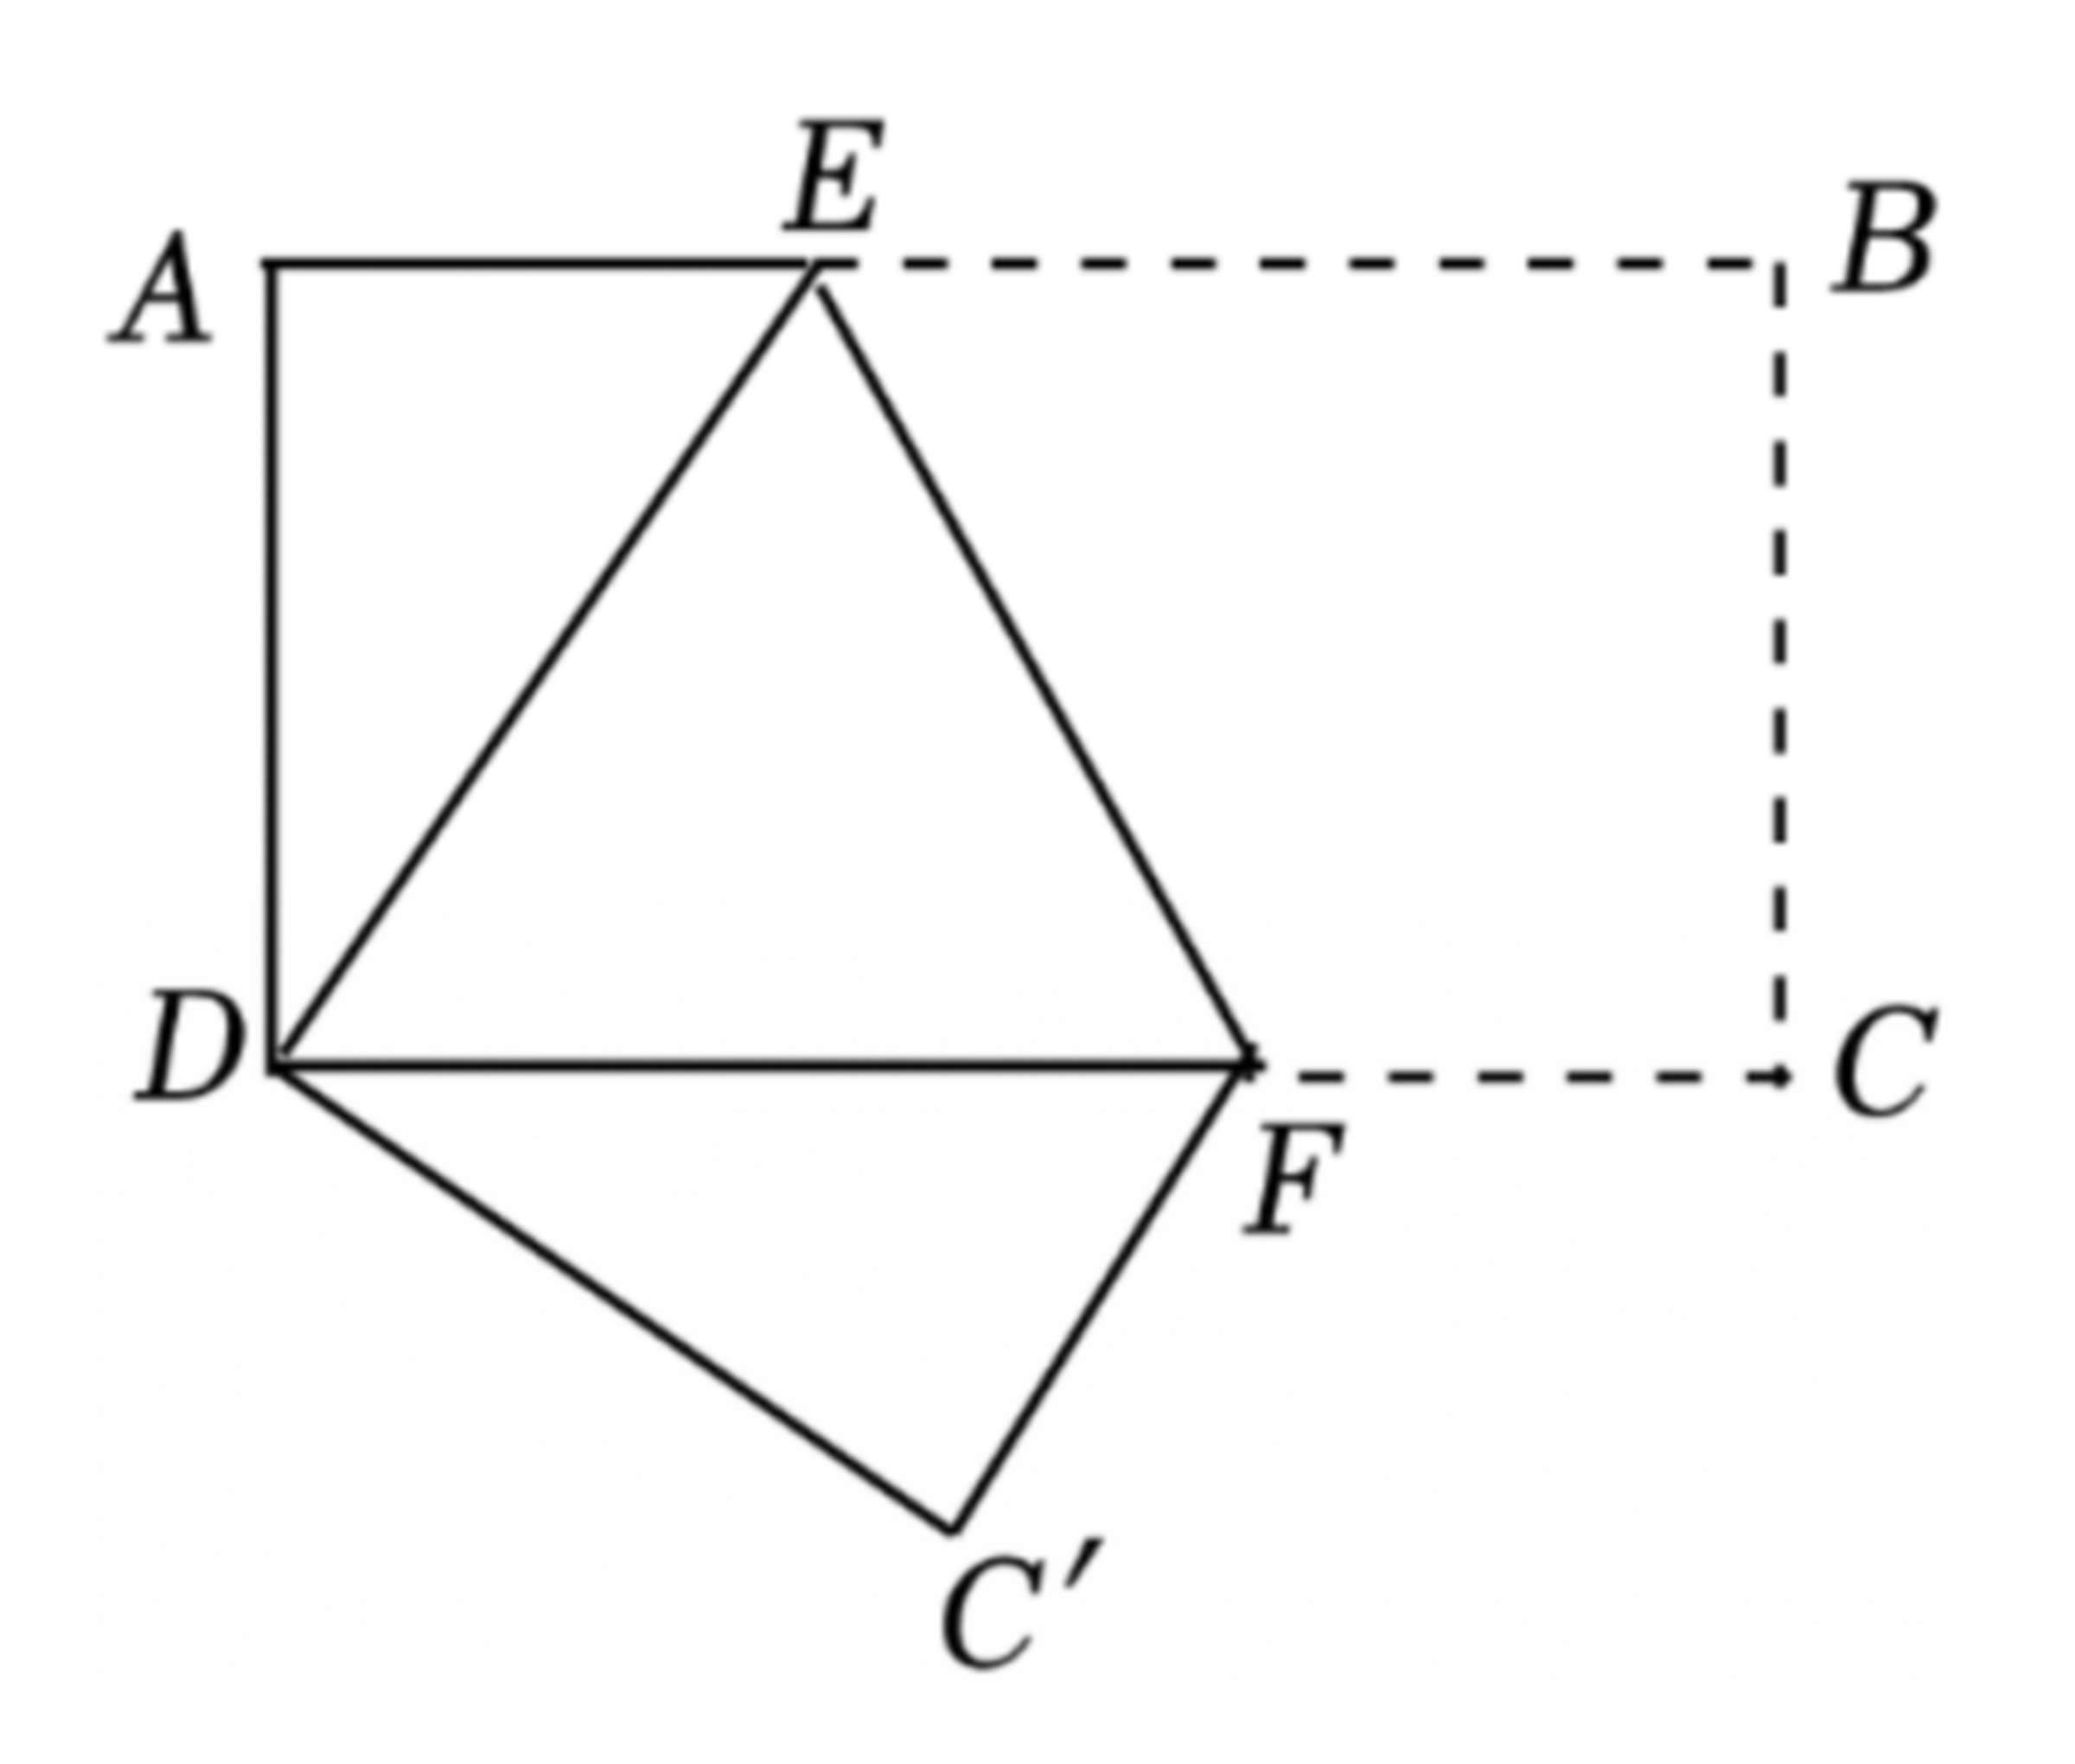
\includegraphics[width=0.40\textwidth]{figures/gao149_q11.png}
\end{center}

\ifanswer
\solbegin
\step{因为矩形 $ABCD(AB>AD)$ 的周长为 12，}
\step{在 $AB$ 和 $CD$ 边上分别取点 $E$ 和 $F$，将四边形 $BCFE$ 沿 $EF$ 折叠，}
\step{使点 $B$ 与点 $D$ 重合，此时点 $C$ 的对应点为 $C'$，}
\step{所以设 $AD=a$，$AB=b$，则 $2(a+b)=12$，}
\step{所以 $a+b=6$，且 $AB>AD$，所以 $b>a>0$，}
\step{设 $DF=x$，则 $C'F=b-x$，在 $Rt\triangle DC'F$ 中，$DC'=BC=a$，}% 几何三角形符号原卷印扁等边细线三角 $\triangle$，照录（放大 02 页确认）；$Rt$ 照录
\step{所以 $a^2+(b-x)^2=x^2$，解得 $x=\dfrac{a^2+b^2}{2b}$，}
\step{因此 $\triangle C'DF$ 的面积 $S=\dfrac{1}{2}\cdot DC'\cdot C'F=\dfrac{1}{2}\cdot a\cdot(b-x)$，}
\step{又 $b-x=b-\dfrac{(6-b)^2+b^2}{2b}=\dfrac{6(b-3)}{b}$，}
\step{所以 $S=\dfrac{1}{2}\cdot a\cdot\dfrac{6(b-3)}{b}=\dfrac{1}{2}\cdot(6-b)\cdot\dfrac{6(b-3)}{b}=\dfrac{3(6-b)(b-3)}{b}$}
\step{$=3\cdot\left(-b-\dfrac{18}{b}+9\right)$，又 $b+\dfrac{18}{b}\geqslant2\sqrt{b\cdot\dfrac{18}{b}}=6\sqrt{2}$，}
\step{当且仅当 $b=\dfrac{18}{b}$ 即 $b=3\sqrt{2}$ 时取等号，此时满足 $b>a$，}
\step{所以 $S\leqslant3\cdot(-6\sqrt{2}+9)=27-18\sqrt{2}$，故 $\triangle C'DF$ 面积的最大值为 $27-18\sqrt{2}$.}
\solend
\fi

% === Q12 === 解析内 3 幅三次函数曲线坐标图（仅答案版出）；解析 15 行（8 行 03 页＋7 行 04 页）
\item 已知 $m>0$，若存在 $t\in\R$，使得对任意 $x\in[0,m]$，不等式 $[(x-1)^2-t](x-t)\leqslant0$ 恒成立，则 $m$ 的最大值是\blankline[4.4em].

\ifanswer
\solbegin
\step{当 $t\leqslant0$ 时，$(x-1)^2-t\geqslant0$ 恒成立，}
\step{不等式 $[(x-1)^2-t](x-t)\leqslant0$ 的解集为 $x\leqslant t$，与 $x\in[0,m]$ 矛盾；}
\step{当 $t>0$ 时，不等式 $[(x-1)^2-t](x-t)\leqslant0\Leftrightarrow(x-1-\sqrt t)(x-1+\sqrt t)(x-t)\leqslant0$，}
\step{若 $t<1-\sqrt t$，即 $t\in\left(0,\dfrac{3-\sqrt5}{2}\right)$，}
\begin{center}
% 情形一 $t<1-\sqrt t$ 曲线图取 03 页右侧，去粉色水印、去色、4× LANCZOS 放大；仅答案版出
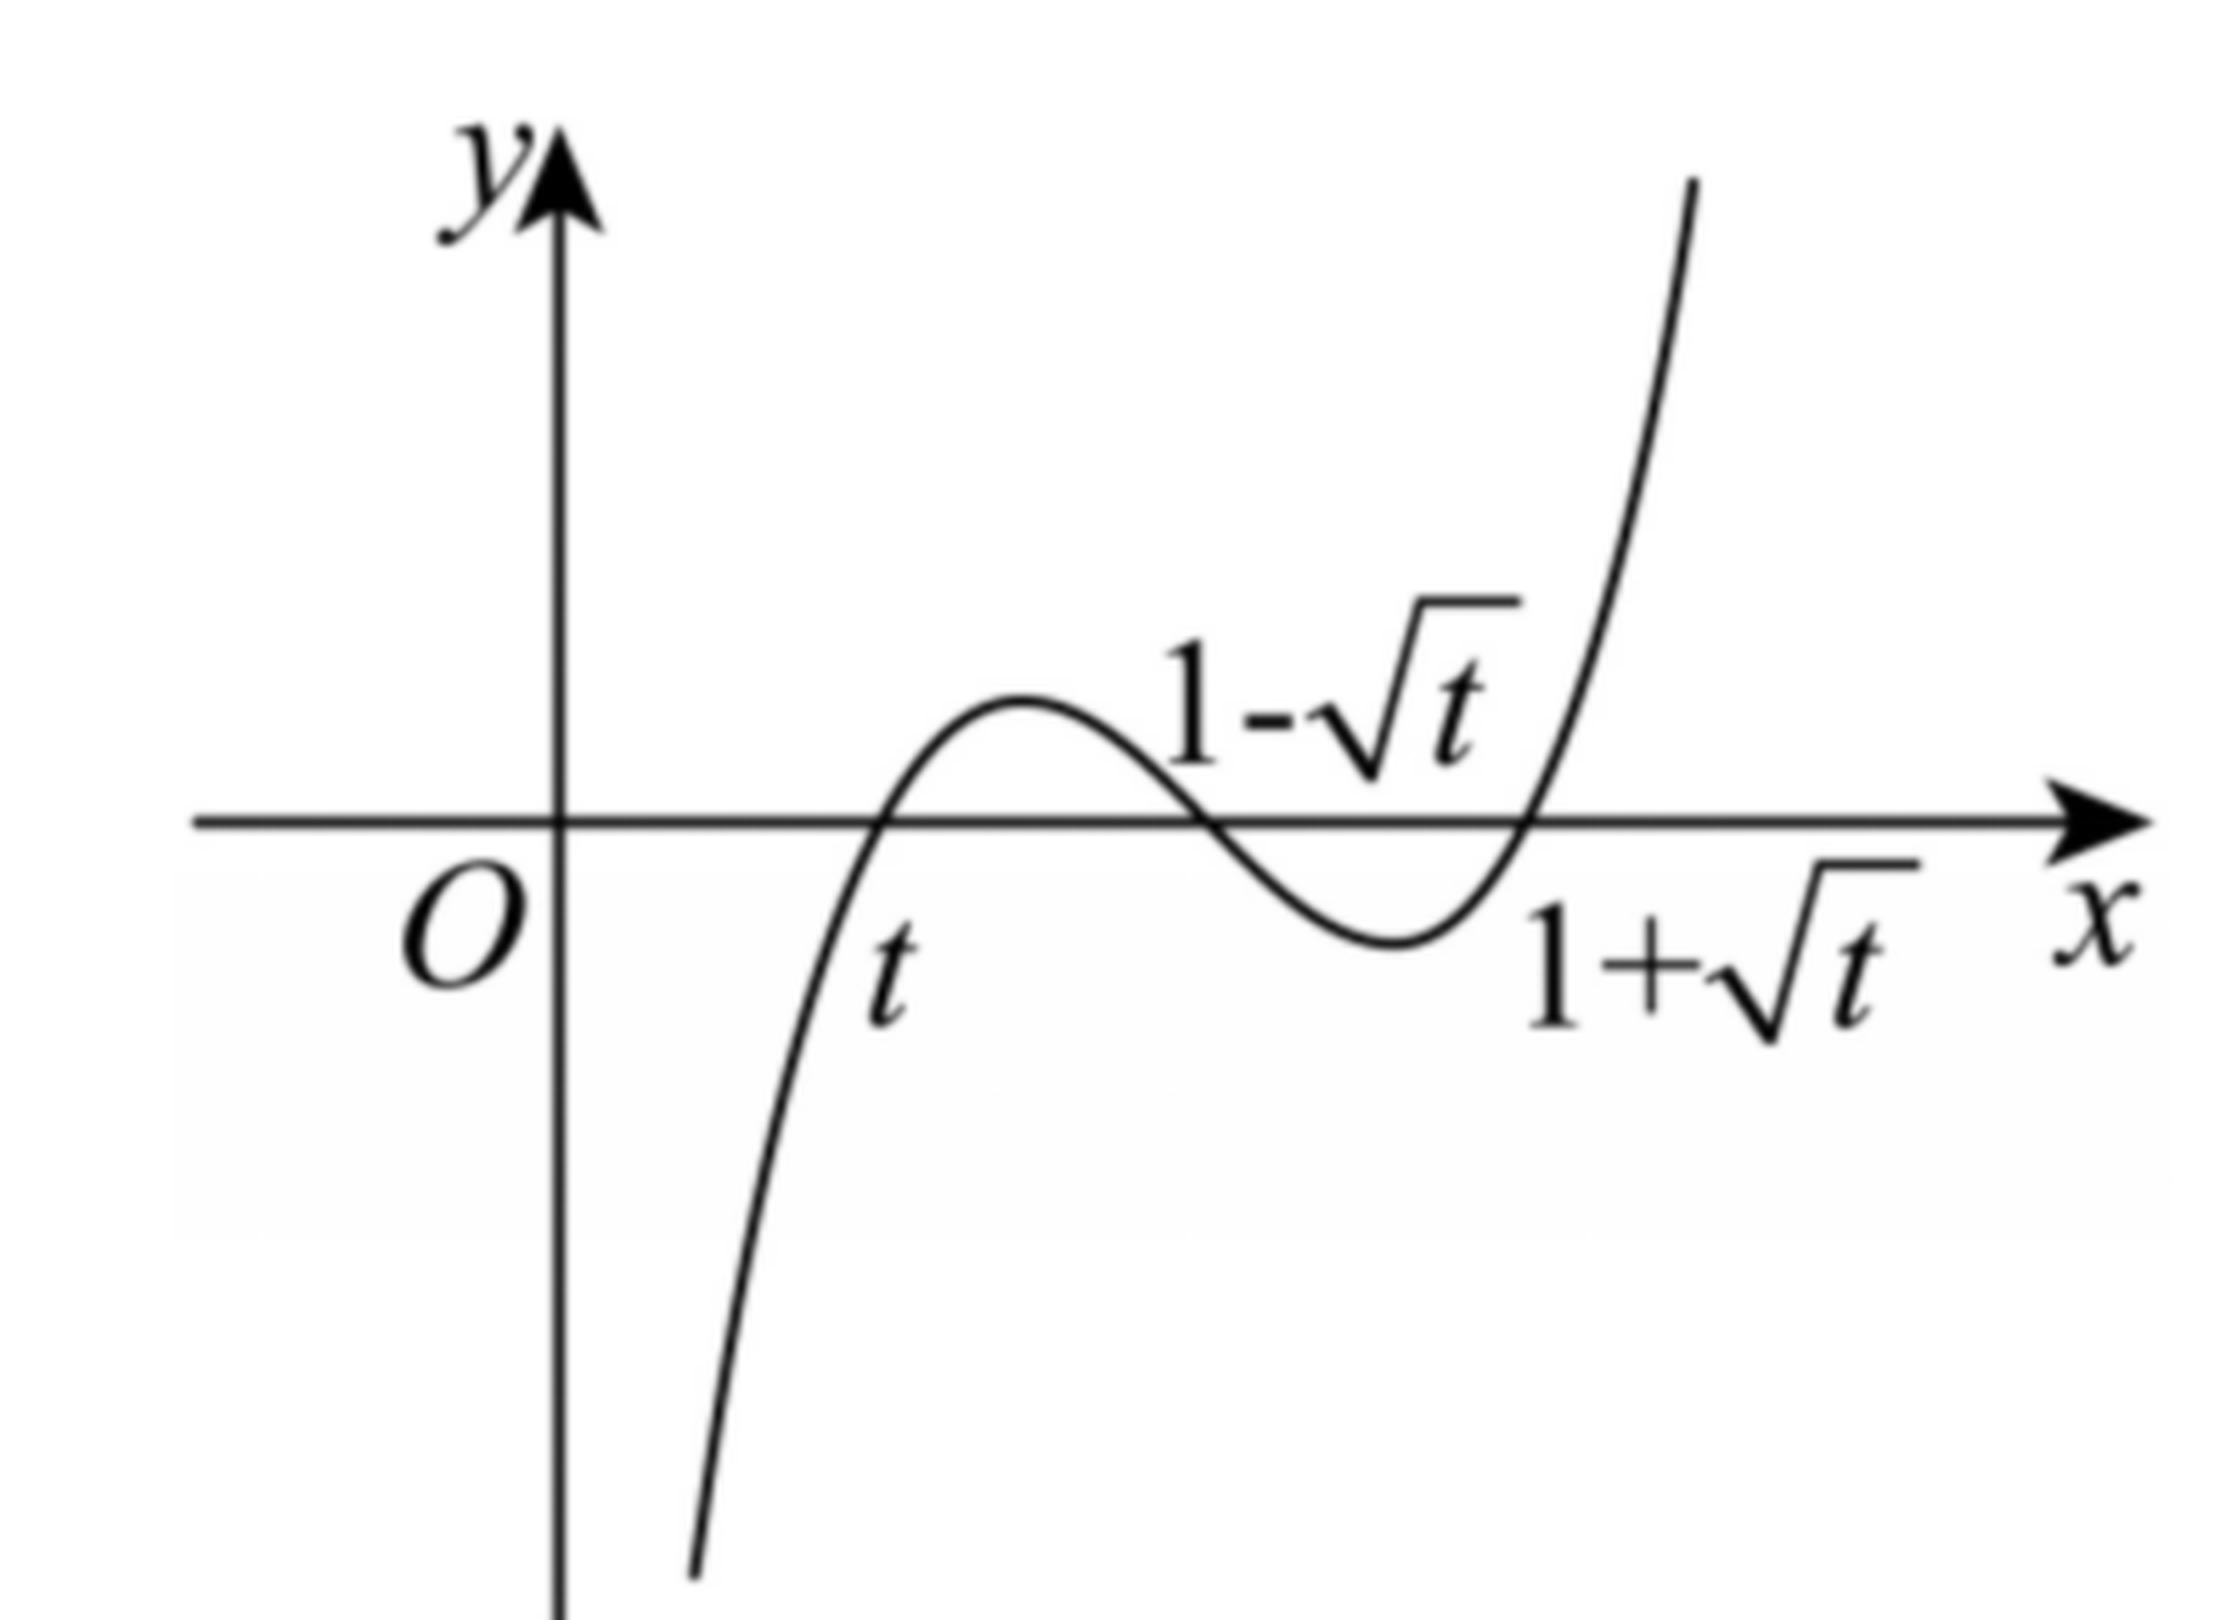
\includegraphics[width=0.40\textwidth]{figures/gao149_q12_a.png}
\end{center}
\step{则原不等式的解集为 $(-\infty,t]\cup[1-\sqrt t,1+\sqrt t]$，}
\step{当 $0<m\leqslant t$ 时，原不等式恒成立，因此}
\step{$m\in\left(0,\dfrac{3-\sqrt5}{2}\right)$；}
\step{若 $t=1-\sqrt t$，即 $t=\dfrac{3-\sqrt5}{2}$，则原不等式的解集为 $(-\infty,1+\sqrt t]$，}
\begin{center}
% 情形二 $t=1-\sqrt t$ 曲线图取 03 页右侧，去粉色水印、去色、4× LANCZOS 放大；仅答案版出
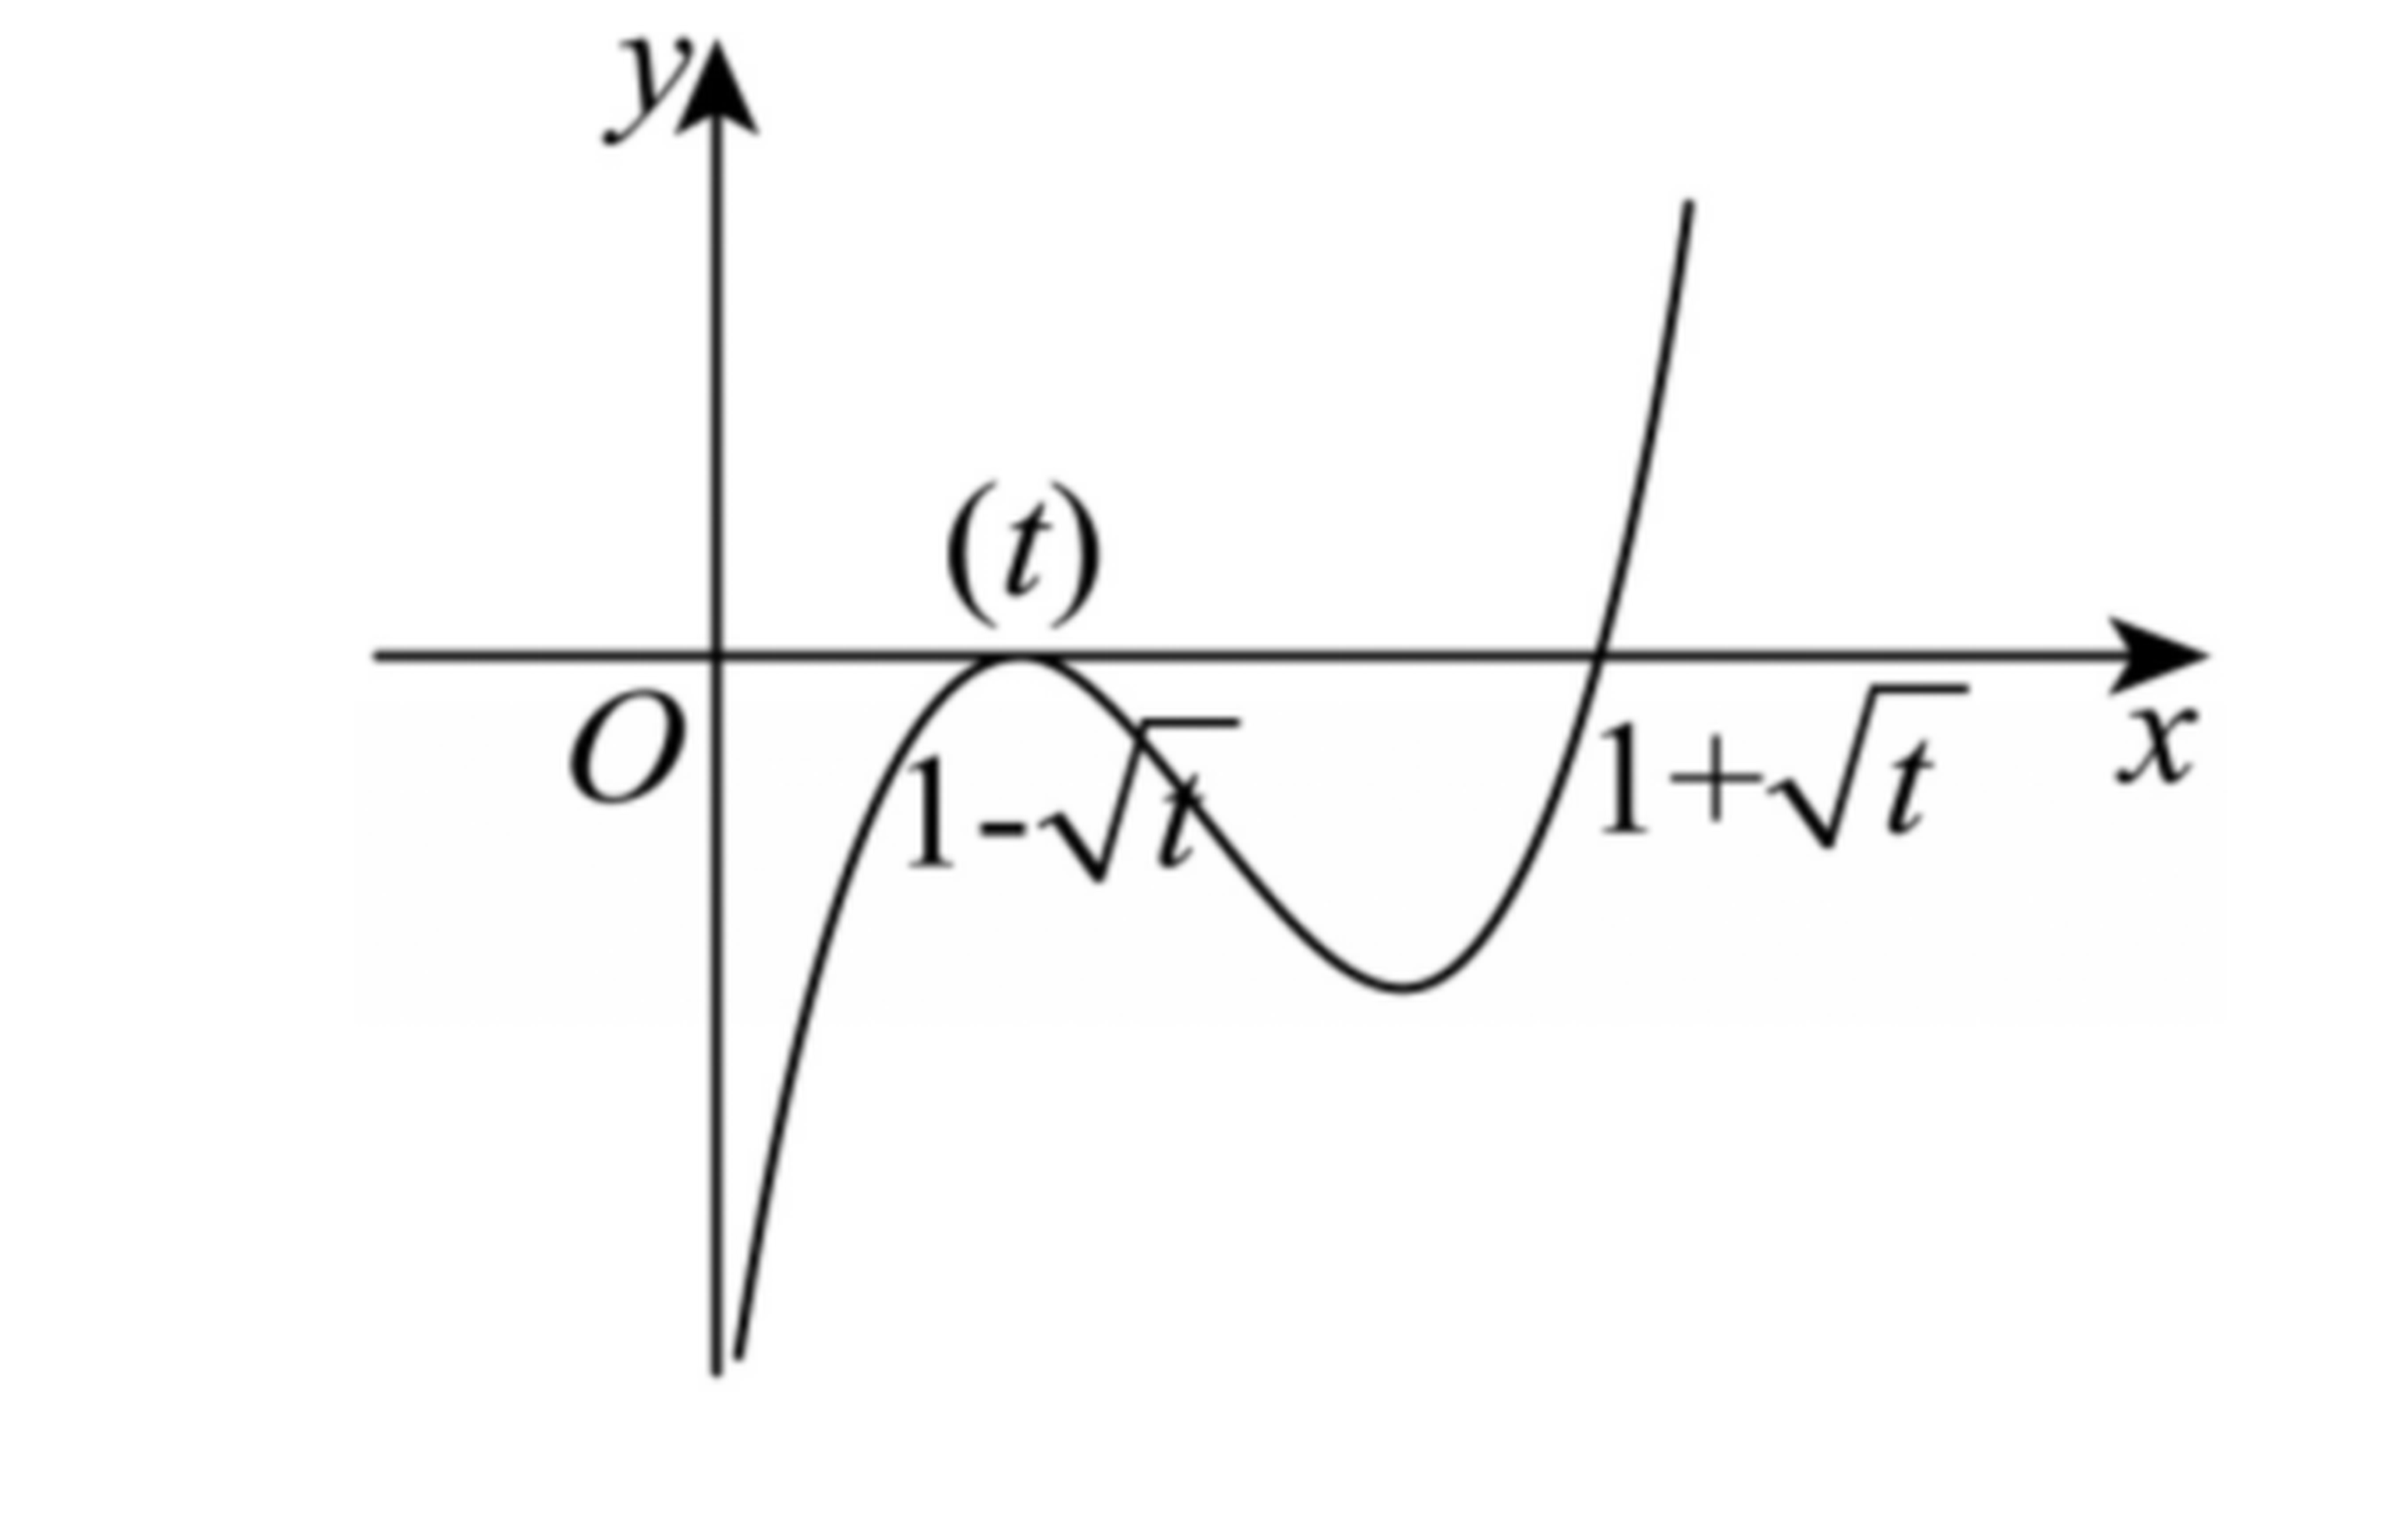
\includegraphics[width=0.40\textwidth]{figures/gao149_q12_b.png}
\end{center}
\step{当 $0<m\leqslant1+\sqrt t$ 时，原不等式恒成立，因此 $m\in\left(0,\dfrac{\sqrt5+1}{2}\right]$；}
\step{若 $1+\sqrt t>t>1-\sqrt t$，即 $t\in\left(\dfrac{3-\sqrt5}{2},\dfrac{3+\sqrt5}{2}\right)$，}
\begin{center}
% 情形三 $1+\sqrt t>t>1-\sqrt t$ 曲线图取 04 页右侧，去粉色水印、去色、4× LANCZOS 放大；仅答案版出
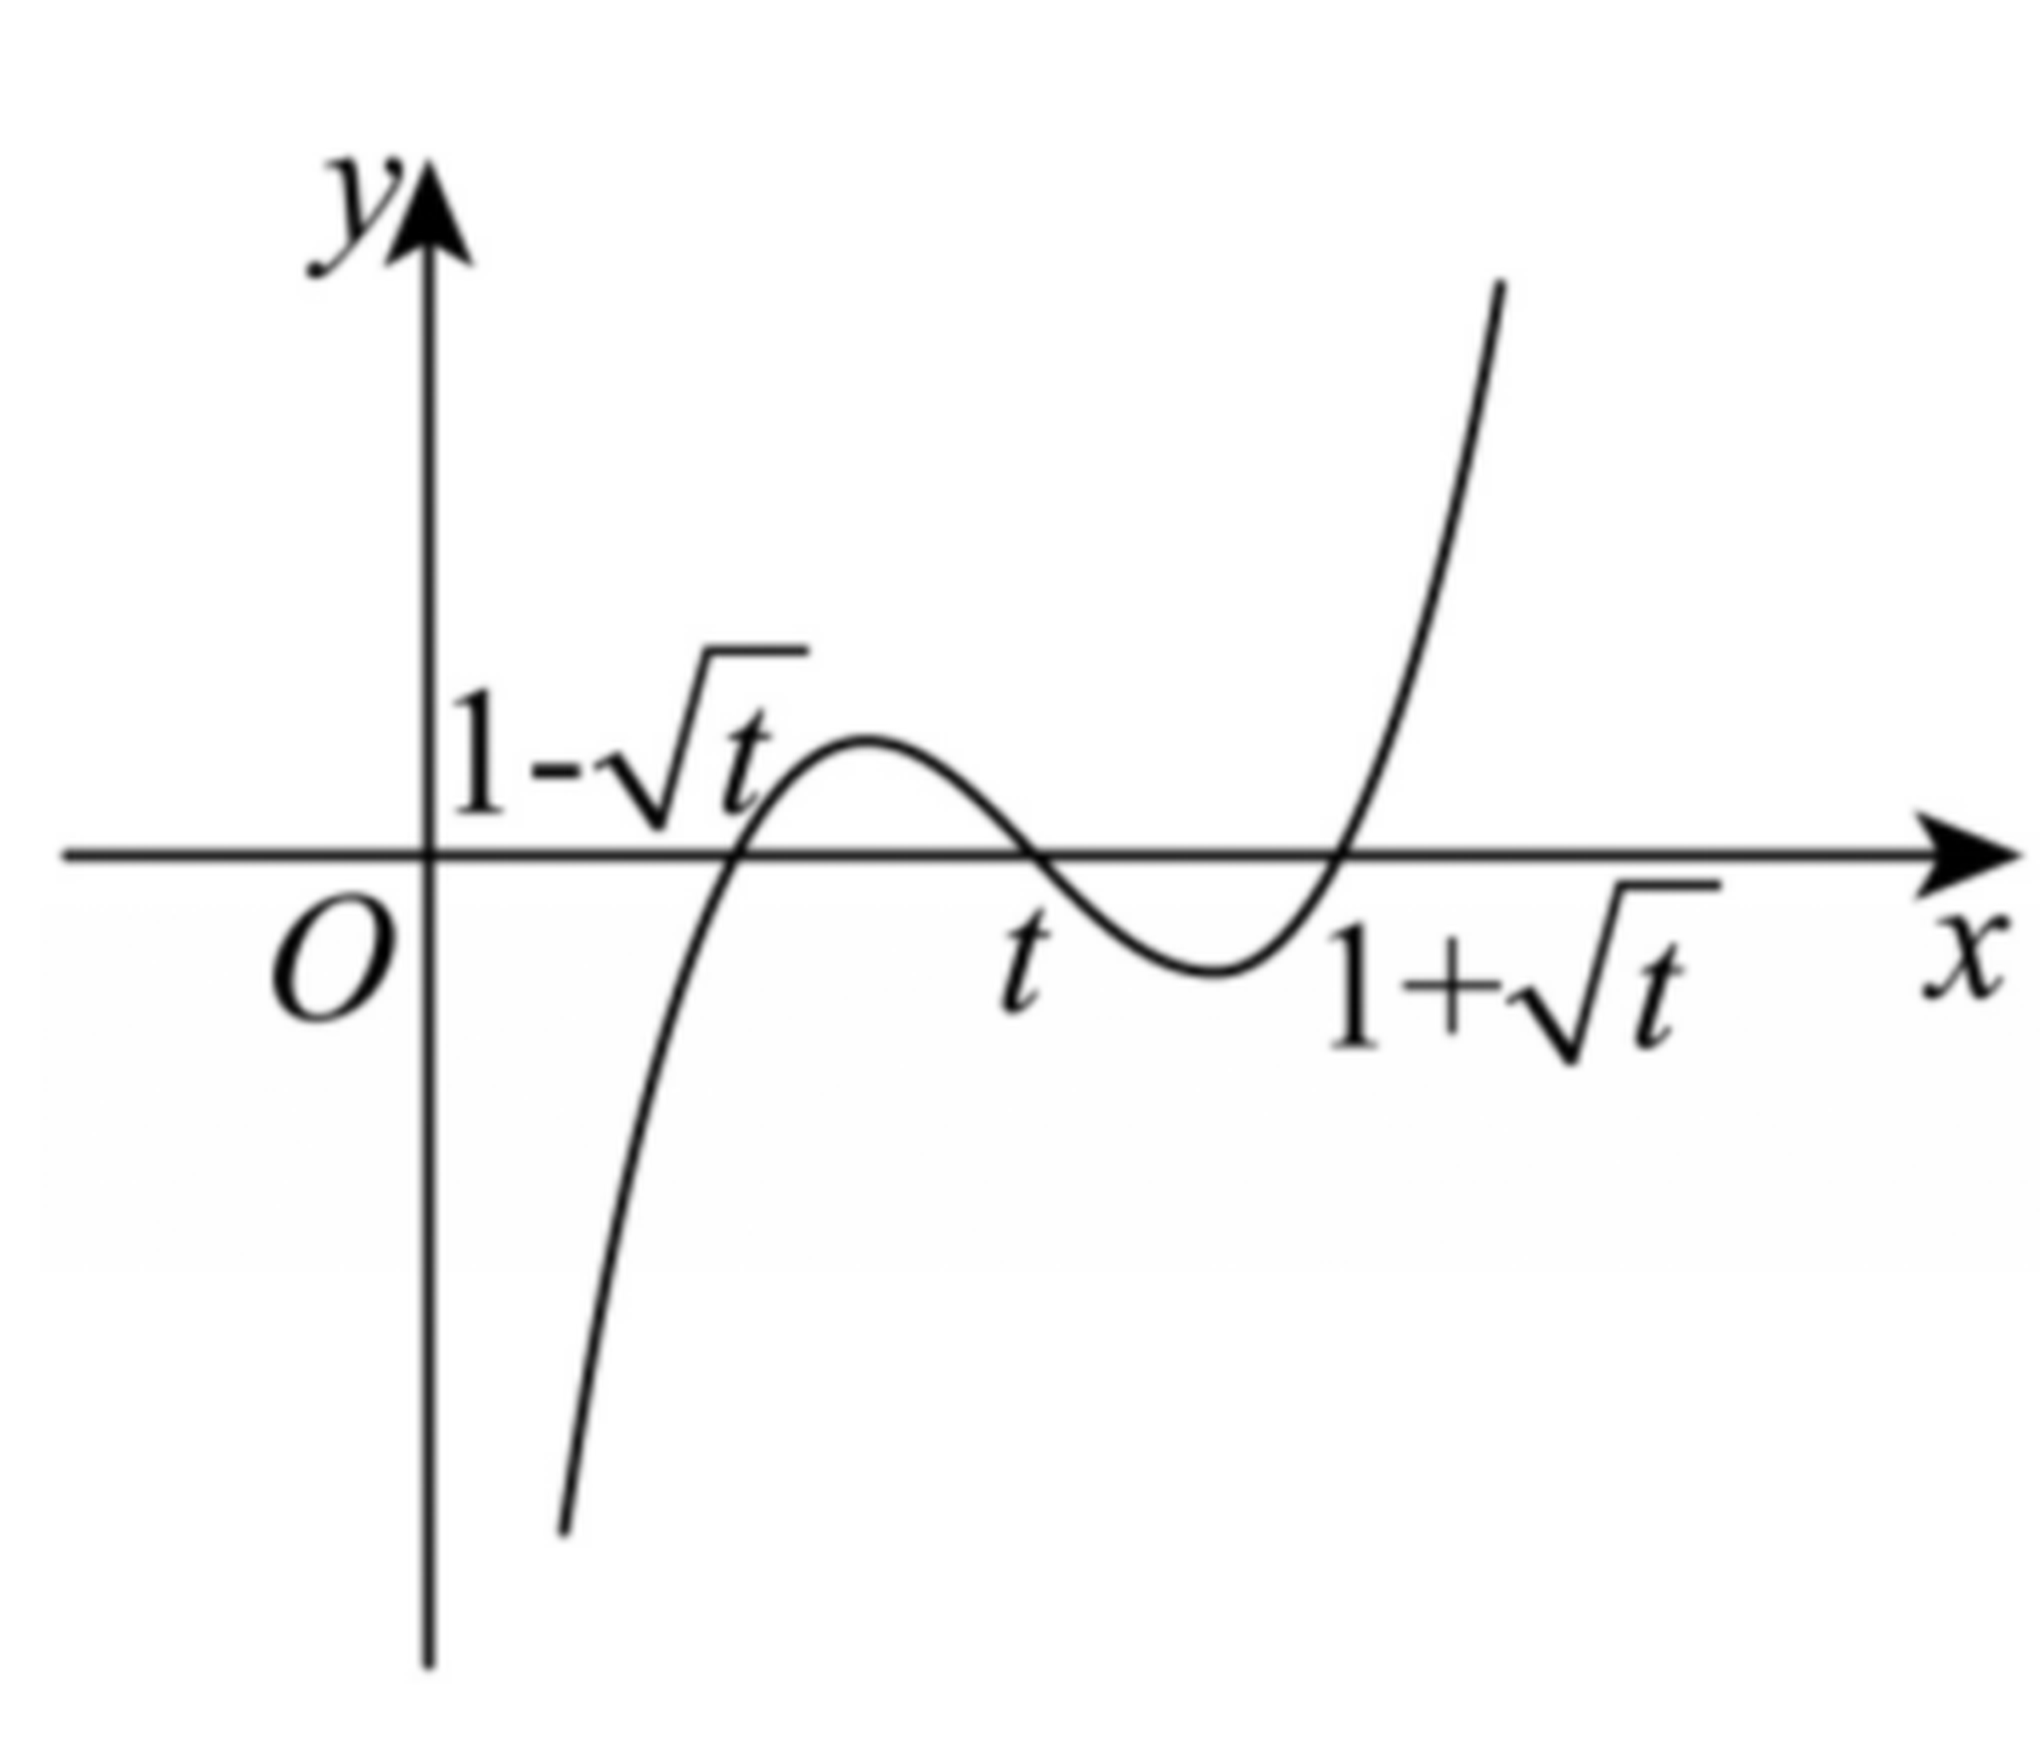
\includegraphics[width=0.40\textwidth]{figures/gao149_q12_c.png}
\end{center}
\step{则原不等式的解集为 $(-\infty,1-\sqrt t]\cup[t,1+\sqrt t]$，}
\step{当 $\begin{cases}1-\sqrt t>0\\1-\sqrt t\geqslant m\end{cases}$ 时，原不等式恒成立，此时 $t\in\left(\dfrac{3-\sqrt5}{2},1\right)$，$m\in\left(0,\dfrac{3-\sqrt5}{2}\right)$；}
\step{若 $t\geqslant1+\sqrt t$，即 $t\geqslant\dfrac{3+\sqrt5}{2}$，则取 $x=0$，$(t-1)t>0$，}
\step{原不等式不恒成立，不符合题意，}
\step{因此实数 $m$ 的取值范围是 $\left(0,\dfrac{\sqrt5+1}{2}\right]$，$m$ 的最大值是 $\dfrac{\sqrt5+1}{2}$.}
\solend
\fi

\end{enumerate}

\bigsec{二、选择题}

\begin{enumerate}
\setcounter{enumi}{12}

% === Q13 ===：答案"C"直接印在题干括号内、无【答案】/【解析】段，按 高一84 Q13／高一148 Q13 成例括号留空、另提 \ans{$C$}；四选项两行两列照原卷分行
\item 设 $ab>0$，则 $a>b$ 是 $\dfrac{1}{a}<\dfrac{1}{b}$ 的\mbox{（\quad）}

\keepwithprev
A. 充分不必要条件\qquad\qquad B. 必要不充分条件

C. 充要条件\qquad\qquad D. 既不充分又不必要条件

\ifanswer
\ans{$C$}
\fi

% === Q14 ===：$A\subset B$ 单线照录；四选项补集照原卷上划线 \overline{A}／\overline{B}；解析 1 行（由韦恩图得 B 对）
\item 已知集合 $A$、$B$ 非空，且 $A\subset B$，则下列式子中一定是空集的为\mbox{（\quad）}

\keepwithprev
A. $\overline{A}\cap B$\qquad B. $A\cap\overline{B}$\qquad C. $\overline{A}\cap\overline{B}$\qquad D. $\overline{A}\cup\overline{B}$

\ifanswer
\solbegin
\step{由韦恩图得 $B$ 对. 故选 $B$.}
\solend
\fi

% === Q15 ===："天文数字"弯引号照录；解析 2 行（首行在 04 页末、末行续 05 页顶）
\item 历史上数学计算方面的三大发明是阿拉伯数字、十进制和对数，其中对数的发明，大大缩短了计算时间，为人类研究科学和了解自然起了重大作用，对数运算对估算“天文数字”具有独特的优势. $2.5^{1000}$ 的估算值约为\mbox{（\quad）}

\keepwithprev
A. $10^{365}$\qquad B. $10^{379}$\qquad C. $10^{389}$\qquad D. $10^{398}$

\ifanswer
\solbegin
\step{$\lg 2.5^{1000}=1000\lg 2.5=1000(1-2\lg 2)\approx1000\times(1-0.602)=398$，}
\step{所以 $2.5^{1000}\approx10^{398}$. 故选 $D$.}
\solend
\fi

% === Q16 ===："完美集"新定义、圈数字①②文本模式；题干"若对任意 $x$，$y\in A$"用全角逗号、解析用顿号"$x$、$y\in A$"，两处照录不统一；解析 9 行
\item 设全集 $U=\R$，集合 $A$ 是一个非空数集，若对任意 $x$，$y\in A$，都有 $x+y\in A$、$xy\in A$，则称集合 $A$ 为一个“完美集”，给出以下命题：

①若 $A_1$、$A_2$ 都是“完美集”，且 $A_1\cap A_2\ne\varnothing$，则 $A_1\cap A_2$ 也是“完美集”；

②若 $A_1$、$A_2$ 都是“完美集”，则 $A_1\cup A_2$ 也是“完美集”.

下列说法正确的是\mbox{（\quad）}

\keepwithprev
A. ①②都是真命题\qquad\qquad B. ①是真命题，②是假命题

C. ①是假命题，②是真命题\qquad\qquad D. ①②都是假命题

\ifanswer
\solbegin
\step{由题意，全集 $U=\R$，集合 $A$ 是一个非空数集，}
\step{若对任意 $x$、$y\in A$，都有 $x+y\in A$、$xy\in A$，则称集合 $A$ 为一个“完美集”，}
\step{对于①，取 $x$、$y\in A_1\cap A_2$，则 $x\in A_1$，$x\in A_2$，$y\in A_1$，$y\in A_2$，}
\step{又 $A_1$、$A_2$ 是“完美集”，所以 $x+y\in A_1$，$xy\in A_1$，$x+y\in A_2$，$xy\in A_2$，}
\step{所以 $x+y\in A_1\cap A_2$，$xy\in A_1\cap A_2$，所以 $A_1\cap A_2$ 是“完美集”，故①正确；}
\step{对于②，取“完美集” $A_1=\{x\mid x=2k,k\in\Z\}$，$A_2=\{x\mid x=3k,k\in\Z\}$，}
\step{则 $2\in A_1$，$3\in A_2$，但 $2+3\notin A_1\cup A_2$，}
\step{即此时 $A_1\cup A_2$ 不是“完美集”，故②错误.}
\step{故选 $B$.}
\solend
\fi
\end{enumerate}

\bigsec{三、解答题}

\begin{enumerate}
\setcounter{enumi}{16}

% === Q17 ===："图像"（有亻）照录（Q17 题干与解析共 2 处）；绝对值 \lvert…\rvert；解析 7 行
\item 已知 $m\in\R$，$f(x)=(m^2-m-5)x^m$. 若 $y=f(x)$ 是幂函数，且其图像不经过原点.

(1) 求实数 $m$ 的值；

(2) 若 $f(a)=f(b)$ 且 $a\ne b$，求 $\lvert a+2\rvert+\lvert b-1\rvert$ 的最小值，并指出取到最小值时 $a$ 的取值范围.

\ifanswer
\solbegin
\step{(1) $f(x)=(m^2-m-5)x^m$ 是幂函数，得 $m^2-m-5=1$，即 $m^2-m-6=0$，}
\step{解得 $m=-2$ 或 $m=3$，又函数图像不经过原点，所以 $m=-2$($3$ 舍)；}
\step{(2) 由 (1) 得 $f(x)=x^{-2}=\dfrac{1}{x^2}$ 为偶函数，}
\step{$x<0$ 时，函数 $f(x)$ 严格增，$x>0$ 时，函数 $f(x)$ 严格减，}
\step{又 $f(a)=f(b)$ 且 $a\ne b$，所以 $a=-b$，且 $a\ne0$，$b\ne0$，}
\step{则 $\lvert a+2\rvert+\lvert b-1\rvert=\lvert a+2\rvert+\lvert-a-1\rvert=\lvert a+2\rvert+\lvert a+1\rvert$，}
\step{则 $\lvert a+2\rvert+\lvert b-1\rvert$ 的最小值为 $1$，取到最小值时 $a$ 的取值范围是 $[-2,-1]$.}
\solend
\fi

% === Q18 ===：判别式两形混用——(1) cases 块印高 \Delta、(2) 独立行印扁 \triangle，逐处照录不统一；解析 8 行
\item 已知命题 $p$：方程 $x^2+4x+m-1=0$ 有两个不等的负根；命题 $q$：方程 $4x^2+4x+m-2=0$ 无实根.

(1) 若 $p$ 为真命题，求 $m$ 的取值范围；

(2) 若 $p$、$q$ 两命题一真一假，求 $m$ 的取值范围.

\ifanswer
\solbegin
\step{(1) 若 $p$ 为真命题，即方程 $x^2+4x+m-1=0$ 有两个不等的负根；}
\step{必有 $\begin{cases}\Delta=16-4(m-1)>0\\m-1>0\end{cases}$，解得 $1<m<5$，即 $m$ 的取值范围为 $(1,5)$；}
\step{(2) 命题 $q$：方程 $4x^2+4x+m-2=0$ 无实根，}
\step{则有 $\triangle=16-16(m-2)<0$，解得 $m>3$，}
\step{若 $p$ 和 $q$ 有且只有一个为真命题，}
\step{若 $p$ 真 $q$ 假，必有 $\begin{cases}1<m<5\\m\leqslant3\end{cases}$，则有 $1<m\leqslant3$，}
\step{若 $p$ 假 $q$ 真，必有 $\begin{cases}m\leqslant1\text{ 或 }m\geqslant5\\m>3\end{cases}$，则有 $m\geqslant5$，}
\step{综上，$1<m\leqslant3$ 或 $m\geqslant5$.}
\solend
\fi

% === Q19 ===：$A\subseteq B$ 带下划线照录；解析 7 行（(2) 两组 cases 并排）
\item 已知 $m\in\R$，集合 $A=\left\{x\mid y=\sqrt{3-x}-\dfrac{1}{\sqrt{x-1}}\right\}$，集合 $B=\{x\mid 2m\leqslant x\leqslant1-m\}$.

(1) 若 $A\cup B=B$，求实数 $m$ 的取值范围；

(2) 若 $A\cap B=\varnothing$，求实数 $m$ 的取值范围.

\ifanswer
\solbegin
\step{(1) 函数 $y=\sqrt{3-x}-\dfrac{1}{\sqrt{x-1}}$，则 $\begin{cases}3-x\geqslant0\\x-1>0\end{cases}$，解得 $1<x\leqslant3$，}
\step{所以 $A=\{x\mid1<x\leqslant3\}$，}
\step{因为 $A\cup B=B$，所以 $A\subseteq B$，则 $\begin{cases}2m\leqslant1\\1-m\geqslant3\end{cases}$，解得 $m\leqslant-2$，}
\step{综上，实数 $m$ 的取值范围为 $(-\infty,-2]$；}
\step{(2) 当 $B=\varnothing$ 时，则 $2m>1-m$，解得 $m>\dfrac{1}{3}$，}
\step{当 $B\ne\varnothing$ 时，则 $\begin{cases}2m\leqslant1-m\\2m>3\end{cases}$ 或 $\begin{cases}2m\leqslant1-m\\1-m\leqslant1\end{cases}$，解得 $m\in\varnothing$ 或 $0\leqslant m\leqslant\dfrac{1}{3}$，}
\step{综上，实数 $m$ 的取值范围为 $[0,+\infty)$.}
\solend
\fi

% === Q20 ===：n 阶基本不等式推广；(3) 解析含 \overbrace{…}^{k} 上括号；(2) 解析"x=x=x=3(1-x)"三连等系原卷笔误、照录加注（见 ⑤）；解析 14 行
\item 教材中的基本不等式可以推广到 $n$ 阶：$n$ 个正数的算术平均数不小于它们的几何平均数，即对于任意的正数 $a_1$、$a_2$、$\cdots$、$a_n$，有 $\dfrac{a_1+a_2+\cdots+a_n}{n}\geqslant\sqrt[n]{a_1\cdot a_2\cdots a_n}$（$n\in\N$ 且 $n\geqslant2$），且等号当且仅当 $a_1=a_2=\cdots=a_n$ 时成立. 利用此结论解决下列问题：

(1) 若 $x$、$y$、$z>0$，求 $\dfrac{y}{x}+\dfrac{2z}{y}+\dfrac{4x}{z}$ 的最小值；

(2) 已知 $0<x<1$，求 $x^3(1-x)$ 的最大值，并求取得最大值时的 $x$ 的值；

(3) 对任意的正整数 $k$，判断 $\left(1+\dfrac{1}{k}\right)^k$ 与 $\left(1+\dfrac{1}{k+1}\right)^{k+1}$ 的大小关系，并证明.

\ifanswer
\solbegin
\step{(1) 因为 $x$、$y$、$z>0$，有 $\dfrac{y}{x}>0$，$\dfrac{2z}{y}>0$，$\dfrac{4x}{z}>0$}
\step{所以 $\dfrac{y}{x}+\dfrac{2z}{y}+\dfrac{4x}{z}\geqslant3\sqrt[3]{\dfrac{y}{x}\cdot\dfrac{2z}{y}\cdot\dfrac{4x}{z}}=3\sqrt[3]{8}=6$，}
\step{当且仅当 $\dfrac{y}{x}=\dfrac{2z}{y}=\dfrac{4x}{z}$ 时取等号，故 $\dfrac{y}{x}+\dfrac{2z}{y}+\dfrac{4x}{z}$ 的最小值为 $6$.}
\step{(2) 因为 $0<x<1$，所以 $1-x>0$，}
\step{$x^3(1-x)=\dfrac{1}{3}[x\cdot x\cdot x\cdot3(1-x)]\leqslant\dfrac{1}{3}\left[\dfrac{x+x+x+3(1-x)}{4}\right]^4=\dfrac{1}{3}\times\left(\dfrac{3}{4}\right)^4$}
\step{$=\dfrac{27}{256}$，当且仅当 $x=x=x=3(1-x)$，即 $x=3(1-x)$，$x=\dfrac{3}{4}$ 取等号，}% 原卷"x=x=x=3(1-x)"三连等，疑为四因子相等之误排，放大 08 页确认，照录未改（见 ⑤）
\step{所以 $0<x<1$ 时，$x^3(1-x)$ 的最大值是 $\dfrac{27}{256}$，取最大值时 $x=\dfrac{3}{4}$.}
\step{(3) 对任意 $k\in\N^*$，$\left(1+\dfrac{1}{k}\right)^k<\left(1+\dfrac{1}{k+1}\right)^{k+1}$.}
\step{证明：$\left(1+\dfrac{1}{k}\right)^k=\overbrace{\left(1+\dfrac{1}{k}\right)\cdot\left(1+\dfrac{1}{k}\right)\cdots\left(1+\dfrac{1}{k}\right)}^{k}\times1$}
\step{$\leqslant\left(\dfrac{\overbrace{\left(1+\dfrac{1}{k}\right)+\left(1+\dfrac{1}{k}\right)+\cdots+\left(1+\dfrac{1}{k}\right)}^{k}+1}{k+1}\right)^{k+1}$}
\step{$=\left(\dfrac{\overbrace{(1+1+\cdots+1)}^{k}+\overbrace{\left(\dfrac{1}{k}+\dfrac{1}{k}+\cdots+\dfrac{1}{k}\right)}^{k}+1}{k+1}\right)^{k+1}=\left(\dfrac{k+1+1}{k+1}\right)^{k+1}=\left(1+\dfrac{1}{k+1}\right)^{k+1}$，}
\step{当且仅当 $1+\dfrac{1}{k}=1$ 时取等号，}
\step{但是任意 $k\in\N^*$ 时 $1+\dfrac{1}{k}>1$，所以等号不成立，}
\step{故任意 $k\in\N^*$ 时，$\left(1+\dfrac{1}{k}\right)^k<\left(1+\dfrac{1}{k+1}\right)^{k+1}$.}
\solend
\fi

% === Q21 ===："减 k 集"新定义（引号内 k／数字两侧空格照录）；解析 26 行（续 10 页），含 ⑤ 三处原卷笔误照录
\item 定义：对于给定的整数 $k$，若非空集合 $A$ 满足如下 3 个条件：

① $A$ 是正整数集的子集；② $A\ne\{1\}$；

③对任意正整数 $x,y$，若 $x+y\in A$，则 $xy-k\in A$；则称集合 $A$ 为“减 $k$ 集”.

(1) 判断集合 $A=\{1,2\}$ 是否为“减 $0$ 集”？是否为“减 $1$ 集”？（无需说明理由）

(2) 证明：不存在“减 $2$ 集”；

(3) 是否存在“减 $1$ 集”？如果存在，求出所有“减 $1$ 集”；如果不存在，说明理由.

\ifanswer
\solbegin
\step{(1) 因为 $P\subseteq\N^*$，$P\ne\{1\}$，$1+1=2\in P$，$1\times1-0\in P$，}
\step{所以集合 $P=\{1,2\}$ 是“减 $0$ 集”；}
\step{因为 $P\subseteq\N^*$，$P\ne\{1\}$，$1+1=2\in P$，$1\times1-1\notin P$，}
\step{所以集合 $P=\{1,2\}$ 是“减 $1$ 集”；}% 按条件③应为"不是"，原卷径印"是"，放大 09 页确认，照录未改（见 ⑤）
\step{(2) 假设存在集合 $A$ 是“减 $2$ 集”，若 $x+y\in A$，则 $xy-2\in A$，}
\step{①当 $x+y=xy-2$ 时，有 $(x-1)(y-1)=3$，}
\step{则 $x$、$y$ 一个为 $2$，一个为 $4$，所以集合 $A$ 有元素 $6$，}
\step{但 $3+3\in A$，$3\times3-2\notin A$，与 $A$ 是“减 $2$ 集”矛盾；}
\step{②当 $x+y\ne xy-2$ 时，则 $x+y=xy-1$ 或 $x+y=xy-m$($m>2$)，}
\step{若 $x+y=xy-1$，$m=1$ 时，$M$ 为除 $1$ 以外的最小元素，}% 原卷"m=1"上文未显式定义，疑笔误，放大 09 页确认，照录未改（见 ⑤）
\step{则 $x=M-1$，$y=1$ 时，$xy-2=M-3$ 小于 $M$，}
\step{要符合题意，必须 $M=4$，}
\step{此时取 $x-2$，$y=2$，$xy-2=2$ 不属于 $A$，故不符合题意，}% 原卷"取 x−2"疑为"取 x=2"误排，放大 09 页确认，照录未改（见 ⑤）
\step{当 $m>2$ 时，$(x-1)(y-1)=m+1$，同样得出矛盾，}
\step{综上，不存在 $A$ 是“减 $2$ 集”.}
\step{(3) 存在“减 $1$ 集” $A$，则 $A\ne\{1\}$，}
\step{①假设 $1\in A$，则 $A$ 中除了元素 $1$ 以外，必然还含有其它元素，}
\step{假设 $2\in A$，$1+1\in A$，而 $1\times1-1\notin A$，所以 $2\notin A$，}
\step{假设 $3\in A$，$1+2\in A$，而 $1\times2-1\in A$，所以 $3\in A$，}
\step{所以 $A=\{1,3\}$，}
\step{假设 $4\in A$，$1+3\in A$，而 $1\times3-1\notin A$，所以 $4\notin A$，}
\step{假设 $5\in A$，$1+4\in A$，$1\times4-1\in A$，$2+3=5$，$2\times3-1\in A$，所以 $5\in A$，}
\step{所以 $A=\{1,3,5\}$，}
\step{以此类推，得 $A=\{1,3,5,\cdots,2n-1,\cdots\}$，($n\in\N^*$)，}
\step{所以所有的“减 $1$ 集”有 $\{1,3\}$，$\{1,3,5\}$，$\{1,3,5,7\}$，$\cdots$，$\{1,3,5,\cdots,2n-1,\cdots\}$，}
\step{$(n\in\N^*)$.}
\solend
\fi
\end{enumerate}

\end{document}
"
%
% ① 原始材料：微信公众号"魔都数学加油站"文章，连载"27学年高一149"，原文标题
% "27学年高一149——2026-2027年上海市青浦高级中学上外云间高一上期中"；
% 原文链接：https://mp.weixin.qq.com/s/T7_nyoR1k0o_5og7FkDsyw 。
% 正文为 10 张 PNG 页（01/02/03/04/10 为 2560×3620，05/06/07/08/09 为 4762×6735，
% 同一篇各页分辨率混排，逐页按各自分辨率裁图核对，别按预览比例换算裁框）。
% 体例：混合体例讲评版——19 题中 Q6 只印【答案】、无【解析】；Q13 的答案"C"
%   直接印在题干括号内、无【答案】/【解析】段；其余 17 题印【解析】（逐题核实，见 ② ②）。
% 题目、答案、解析均据原图转录；卷面粉红色水印"魔都数学加油站"及公众号页脚未录入。
% 全卷插图清单（逐页通读 10 页确认）：1 幅题目配图 + 3 幅【解析】内配图：
%   · Q11 矩形 ABCD 折叠几何图（02 页右侧：A/B/C/D/E/F/C' 与虚线 EB、BC、FC），
%     题干"如图"处，题目配图、三版都出，裁 figures/gao149_q11.png；
%   · Q12【解析】内 3 幅三次函数曲线坐标图（03 页右侧两幅 + 04 页右侧一幅：
%     x/y 轴、O、t、1-\sqrt t、1+\sqrt t 等标注，分别对应 t<1-\sqrt t、
%     t=1-\sqrt t、1+\sqrt t>t>1-\sqrt t 三种情形），解析配图、仅答案版出，
%     分别裁 figures/gao149_q12_a.png／_b.png／_c.png，放 \ifanswer 内 \step 之间
%     （高一73 第 16 题成例）；
%   其余各页逐页确认无其它题目配图、无表格；Q14 解析"由韦恩图得 B 对"仅文字推导、
%   原卷并未印韦恩图；Q9／Q18／Q19 的 cases 块与 Q20(3) 的 \overbrace 为数学块（非图）；
%   10 页下半仅水印、无正文。4 图均取自原卷截图，去粉色水印、去色、4× LANCZOS 放大。
%
% 卷首标题：原卷印作"2026-2027 年青浦高级中学上外云间高一上期中"，年份区间按全稿
% 惯例排 en dash；原卷卷面未印副标题，本稿按同期中卷（高一140／141／143／144／145／
% 146／147／148）知识模块口径补出"集合与常用逻辑用语、不等式、函数"。
%
% 题号体例（逐页核实定稿）：本卷共 19 题——一、填空题 3—12（10 题）、
% 二、选择题 13—16（4 题）、三、解答题 17—21（5 题）。
% 三节分别 \setcounter{enumi}{2}／{12}／{16}。原卷从第 3 题起、无第 1、2 题，
% 本稿保留原题号；全卷无附加题节（Q21 解析末行"（n\in N^*）."为全卷收尾）。
%
% ② 与原卷的排版差异：
%   ① 原文从第 3 题起，本稿保留原题号；共 19 题三节；
%   ② 混合体例逐题核实：Q6（反证法"假设的内容"）只印【答案】、无【解析】，
%      按 高一140 第 5 题／高一145 Q3 成例提 \ans{}、不补造解析；Q13 答案"C"直接
%      印在题干括号内、全卷无该题【答案】/【解析】段，按 高一84 Q13／高一148 Q13
%      成例括号 \mbox{（\quad）} 留空、另提 \ans{$C$}；其余 17 题印【解析】、
%      用 \solbegin…\solend，选择题答案在解析末句"故选 X"（Q14 选 B、Q15 选 D、
%      Q16 选 B，逐个放大 04/05 页核实）、题干括号留空、不另提 \ans{}；
%      答案版【答案】/【解析】标记数 = 19（2 个 \ans ＋ 17 个 \solbegin）
%      = 全卷题数；
%   ③ 原卷卷面未印副标题，本稿按知识模块口径补出；
%   ④ 原卷填空横线按全稿惯例排 \blankline[4.4em]；选择题括号排 \mbox{（\quad）}、
%      选项段前按惯例加 \keepwithprev；Q13／Q16 四选项为两行两列、Q14／Q15
%      选项为一行，照原卷分行；解答题不留作答区、不加 \anspace（原卷为讲评版）；
%   ⑤ 数集：Q6"a,b\in N"、Q8"x\in R"、Q9"a\in R"／"解集为 R"、Q12"t\in R"、
%      Q16"U=R"、Q17"m\in R"、Q19"m\in R"、Q20"n\in N" 原卷印斜体 R/N，
%      按全稿惯例统一改 \R／\N；Q20(3)、Q21 的 $N^*$ 排 \N^*；Q16 解析
%      "$k\in Z$" 排 \Z。绝对值排 \lvert…\rvert（Q17），集合描述竖线排 \mid
%      （Q19、Q16 解析）；不等号按全稿惯例排 \leqslant／\geqslant；
%      补集照原卷上划线排 \overline{A}／\overline{B}（Q14 四选项）；空集
%      \varnothing（Q16、Q19、Q21）；
%   ⑥ 子集符号逐处照录不统一：Q4 题干"{1,2}⊆A⊂{1,2,3,4,5,6}" 前者印带下划线
%      ⊆、照录 \subseteq，后者印单线 ⊂、照录 \subset；Q10"A⊆{-1,1/2,2,3}"、
%      Q19 解析"A⊆B"、Q21 解析"P⊆N*" 均印带下划线 ⊆、照录 \subseteq；
%      Q14"A⊂B" 印单线 ⊂、照录 \subset（逐处放大 01/02/04/07/09 页确认，见 ④）；
%   ⑦ 子题标号 (1)(2)(3) 半角括号照录；圈数字 ①②③ 在文本模式（Q16 两命题、
%      Q21 三个条件与解析的①②）按 common.sty 划入 CJK 字符类渲染；cases 块整体
%      算一个印刷行；\left…\right 不得拆到不同 $…$ 组；数学式内 CJK 用 \text{}
%      （Q18 解析 cases 块"\text{或}"）；Q11 解析"Rt\triangle DC'F" 的 Rt 照录；
%   ⑧ 题干／解析中的中文弯引号按原卷照录：Q6" 已知 a,b\in N，若 ab 能被 5 整除，
%      那么 a、b 中至少有一个能被 5 整除 "（开引号后紧跟"已知"、闭引号后空格接"时"）、
%      Q15"天文数字"、Q16"完美集"、Q21"减 k 集""减 0 集""减 1 集""减 2 集"
%      （引号内 k／数字两侧有空格），注释内一律 ASCII 引号；
%   ⑨ 半角逗号在数学组之间是全稿惯例、非笔误（Q8"$a>0,a\ne1,x\in\R$"、
%      Q21 题干"$x,y$" 等），逐处照录别改；Q16 题干"若对任意 $x$，$y\in A$"
%      用全角逗号而解析用顿号"$x$、$y\in A$"，两处不同均照录；行末西文句点
%      照录为 ASCII `.`；行中全角逗号／顿号照录；
%   ⑩ "图像／图象"逐处放大核：Q10 题干与解析共 6 处均印"图象"（象，无亻）；
%      Q17 题干"其图像不经过原点"与解析"又函数图像不经过原点" 2 处印"图像"
%      （像，有亻），逐处照录未统一改动（放大 02/05/06 页确认）；
%   ⑪ 判别式 Δ/△ 混用是照录项：Q9 解析 cases 块"Δ=4(a−2)²+16(a−2)<0"、
%      Q18(1) cases 块"Δ=16−4(m−1)>0" 两处印等腰偏高粗三角 \Delta；
%      Q18(2) 独立行"△=16−16(m−2)<0" 印扁等边细线三角 \triangle，
%      逐处放大判断、照录不统一（参照 高一142／144／145／146／148 头注④口径）；
%      另 Q11 题干"△C'DF 面积"与解析 3 处"△"（含"Rt△DC'F"）共 4 处几何
%      三角形符号亦印扁细线三角，照录 \triangle（非判别式，字形同类，见 ④）；
%   ⑫ 一条 \step = 原卷解析的一个印刷行，cases 块整体算一个印刷行；别把原卷折行
%      并起来、别把一行拆多条。Q11 十三行（7 行在 02 页＋6 行在 03 页）、
%      Q12 十五行（8 行在 03 页＋7 行在 04 页）、Q16 九行、Q21 二十六行
%      （续 10 页）均按印刷行逐条断，不丢行；
%   ⑬ 配图：Q11 题目配图（三版都出）放 \item 内题干之后 \begin{center}，
%      大图块加 \needvspace{8cm} 守卫把整块推走（守卫放 \item 之前，见
%      高一145 Q14/Q20 成例与切页审计 B 类坑）；Q12 三幅解析配图（仅答案版出）
%      放 \ifanswer 内 \solbegin…\solend 的 \step 之间；三版切页审计均"合计异常：无"；
%   ⑭ 跨页续印按题合并：Q3/4/5 在 01 页；Q6/7/8 题干与解析在 01 页；
%      Q9 题干在 01 页末、解析 4 行在 02 页顶；Q10 题干＋解析在 02 页；
%      Q11 题干＋图＋解析前 7 行在 02 页、解析后 6 行续 03 页顶；
%      Q12 题干＋解析首行在 03 页末、解析续 7 行在 03 页下半＋7 行在 04 页顶，
%      "二、选择题"标题在 04 页下半；Q13/14 题干＋选项＋Q14 解析在 04 页下半；
%      Q15 题干＋选项＋解析首行在 04 页末、末行"所以 2.5^1000≈10^398. 故选 D."
%      续 05 页顶；Q16 题干＋选项＋解析 9 行在 05 页、"三、解答题"标题＋
%      Q17 题干首句在 05 页末；Q17(2)＋解析 7 行、Q18 题干＋解析前 6 行在 06 页；
%      Q18 解析末 2 行续 07 页顶；Q19 题干＋解析 4 行在 07 页上半、
%      解析续 3 行在 07 页下半；Q20 题干(1) 在 07 页末、题干(2)(3)＋解析(1)(2)
%      在 08 页上半、(3) 解析含 \overbrace 的证明在 08 页下半、末行
%      "故任意 k∈N* 时…"续 09 页顶；Q21 题干＋解析(1)(2)(3) 前段在 09 页、
%      解析(3) 后半 9 行续 10 页上半（10 页下半仅水印、无正文）。
%      本稿按题连排，不丢行、不并折行；
%   ⑮ 原卷解析内无红色"法一／法二"之类小标题，故本卷无 \stepm；水印
%      "魔都数学加油站"红色不录入。
%
% ③ 行数复核：一条 \step／\stepm = 原卷解析的一个印刷行，cases 块作一个印刷行计。
%   逐题数（主会话逐页核对定稿）：Q3：1；Q4：2；Q5：2；Q6：0（只印【答案】、
%   提 \ans{}）；Q7：1；Q8：1；Q9：4；Q10：5；Q11：13；Q12：15；
%   Q13：0（答案印在题干括号内、另提 \ans{}）；Q14：1；Q15：2；Q16：9；
%   Q17：7；Q18：8；Q19：7；Q20：14；Q21：26。
%   合计 118 条 \step（本卷无 \stepm：解析内无红色"法一／法二"类小标题），
%   与原卷逐题印刷行相等。全卷 17 题设 \solbegin…\solend ＋ 2 处 \ans{}，
%   答案版【答案】/【解析】标记数 = 19 = 全卷题数。
%
% ④ 判别式／子集符号结论（逐处放大原图照录、不得统一，主会话像素级复核）：
%   判别式全卷 3 处，两形混用逐处照录不统一（参照 高一142／144／145／146／148 头注④）：
%     · Q9 解析 cases 块"Δ=4(a−2)²+16(a−2)<0" 原卷印等腰偏高粗三角（高>宽、
%       粗笔画），照录 \Delta（放大 02 页 /tmp/gao149/z/t02_q9_delta2.png 确认）；
%     · Q18(1) cases 块"Δ=16−4(m−1)>0" 原卷印等腰偏高粗三角（高>宽、粗笔画），
%       照录 \Delta（放大 06 页 /tmp/gao149/z/t06_q18a.png 确认）；
%     · Q18(2) 独立行"△=16−16(m−2)<0" 原卷印扁等边细线三角（宽>高、细线），
%       照录 \triangle（放大 06 页 /tmp/gao149/z/t06_q18b.png 与 Q18(1) 并排确认）。
%   另 Q11 题干"△C'DF"与解析 3 处"△"（含"Rt△DC'F"）共 4 处几何三角形符号
%     亦印扁等边细线三角，照录 \triangle（放大 02 页
%     /tmp/gao149/z/t02_q11_tri2.png 确认），与 Q9／Q18(1) 判别式 \Delta 两形不统一。
%   子集／补集：Q4 题干"{1,2}⊆A⊂{1,2,3,4,5,6}" 前者带下划线 ⊆、照录 \subseteq，
%     后者单线 ⊂、照录 \subset（放大 01 页 /tmp/gao149/z/t01_q3q4.png 确认）；
%     Q10"A⊆{-1,1/2,2,3}"、Q19 解析"A⊆B"、Q21 解析"P⊆N*" 三处带下划线 ⊆、
%     照录 \subseteq；Q14"A⊂B" 单线 ⊂、照录 \subset（放大 04 页
%     /tmp/gao149/z/t04_q14_sub2.png 确认）；Q14 四选项补集 \overline{A}／\overline{B}
%     照原卷上划线；空集 \varnothing（Q16、Q19、Q21）；Q19／Q16 解析集合描述竖线
%     \mid；数集 \R／\N／\N^*／\Z 归一见 ② ⑤。
%
% ⑤ 存疑照录（放大原图确认，照录未改、正文对应处另有 % 注）：
%   1. Q21 解析(1) 第二组"因为 P⊆N*，P≠{1}，1+1=2∈P，1×1−1∉P，所以集合
%      P={1,2} 是"减 1 集"" —— 按条件③（x=y=1 时 xy−1=0 须∈P）应为"不是"，
%      原卷却径印"是"，放大 09 页 /tmp/gao149/z/t09_q21_sol1.png 确认，照录未改
%      （疑为原卷结论笔误）。
%   2. Q21 解析(2)"此时取 x−2，y=2，xy−2=2 不属于 A" —— 按上下文应为
%      "取 x=2"（x−2 疑为 x=2 的误排），放大 09 页
%      /tmp/gao149/z/t09_q21_sol2.png 确认，照录未改。
%   3. Q21 解析(2)"若 x+y=xy−1，m=1 时，M 为除 1 以外的最小元素" 中 $m=1$
%      上文未显式定义 m（仅"x+y=xy−m(m>2)"中出现），放大 09 页确认，照录未改。
%   4. Q20 解析(2)"当且仅当 x=x=x=3(1−x)" 三个 x 连等，疑为原卷排印（应为
%      四个因子 x,x,x,3(1−x) 相等），放大 08 页
%      /tmp/gao149/z/t08_q20_sol2.png 确认，照录未改。
%   5. Q6 只印【答案】、Q13 答案印题干括号内，两题均无【解析】，按成例提
%      \ans{}、未补造解析（见 ② ②）。
%   6. 判别式 Q9／Q18(1) 高 \Delta 与 Q18(2)／Q11 扁 \triangle 两形混用，逐处
%      照录不统一（见 ④）；"图像／图象" Q10 用"图象"、Q17 用"图像"，
%      逐处照录未统一（见 ② ⑩）。
%   全卷除此 6 类外未发现其它笔误／自相矛盾处。
%
% ⑥ 跨页续印按题合并说明：见 ② ⑭。
%
\documentclass[a4paper,11pt]{article}
\usepackage{common}

\begin{document}

\examtitlest[3]{2026--2027 年青浦高级中学上外云间高一上期中}{集合与常用逻辑用语、不等式、函数}

\bigsec{一、填空题}

\begin{enumerate}
\setcounter{enumi}{2}

% === Q3 === 根式化分数指数幂；解析 1 行
\item 根式 $\sqrt{a\sqrt a}$ 化成分数指数幂是\blankline[4.4em].

\ifanswer
\solbegin
\step{$\sqrt{a\sqrt a}=\sqrt{a\cdot a^{\frac{1}{2}}}=\sqrt{a^{1+\frac{1}{2}}}=\sqrt{a^{\frac{3}{2}}}=a^{\frac{3}{2}\times\frac{1}{2}}=a^{\frac{3}{4}}$.}
\solend
\fi

% === Q4 === 题干两种子集符号逐处照录（\subseteq 带下划线／\subset 单线）；解析 2 行
\item 满足 $\{1,2\}\subseteq A\subset\{1,2,3,4,5,6\}$ 的集合 $A$ 共有\blankline[4.4em]个.

\ifanswer
\solbegin
\step{集合 $A$ 满足 $\{1,2\}\subseteq A\subset\{1,2,3,4,5,6\}$，}% 前者带下划线 $\subseteq$、后者单线 $\subset$，逐处照录不统一（放大 01 页确认）
\step{所以集合 $A$ 的个数为集合 $\{3,4,5,6\}$ 的真子集的个数，即为 $2^4-1=15$ 个.}
\solend
\fi

% === Q5 === 解析 2 行
\item 不等式 $\dfrac{2x+1}{x-1}\leqslant0$ 的解集为\blankline[4.4em].

\ifanswer
\solbegin
\step{不等式 $\dfrac{2x+1}{x-1}\leqslant0$ 可化为 $(2x+1)(x-1)\leqslant0$，且 $x-1\ne0$，解得 $-\dfrac{1}{2}\leqslant x<1$，}
\step{即原不等式的解集为 $\left[-\dfrac{1}{2},1\right)$.}
\solend
\fi

% === Q6 === 原卷只印【答案】、无【解析】，按 高一140 第 5 题／高一145 Q3 成例提 \ans{}、不补造解析；弯引号与空格照录
\item 用反证法证明命题 “已知 $a,b\in\N$，若 $ab$ 能被 5 整除，那么 $a$、$b$ 中至少有一个能被 5 整除” 时，假设的内容应该是\blankline[4.4em].

\ifanswer
\ans{$a$、$b$ 都不能被 5 整除}
\fi

% === Q7 === 解析 1 行
\item 若 $\log_3(\log_4 x)=1$，则 $x=$\blankline[4.4em].

\ifanswer
\solbegin
\step{$\log_3(\log_4 x)=1$，则 $\log_4 x=3$，故 $x=64$.}
\solend
\fi

% === Q8 === 半角逗号在数学组之间照录；解析 1 行
\item 已知 $a>0,a\ne1,x\in\R$，且 $a^{2x}=2$，则 $\dfrac{a^{3x}+a^{-3x}}{a^x+a^{-x}}$ 的值为\blankline[4.4em].

\ifanswer
\solbegin
\step{$\dfrac{a^{3x}+a^{-3x}}{a^x+a^{-x}}=a^{2x}-1+a^{-2x}=2-1+\dfrac{1}{2}=\dfrac{3}{2}$.}
\solend
\fi

% === Q9 === 题干在 01 页末、解析 4 行在 02 页顶；cases 块整体算 1 行；判别式高 \Delta
\item 已知 $a\in\R$，若关于 $x$ 的不等式 $(a-2)x^2+2(a-2)x-4<0$ 的解集为 $\R$，则实数 $a$ 的取值范围是\blankline[4.4em].

\ifanswer
\solbegin
\step{当 $a=2$ 时，不等式化为 $-4<0$ 对于任意实数 $x$ 都成立，因此 $a=2$ 满足题意；}
\step{当 $a\ne2$ 时，要使关于 $x$ 的不等式 $(a-2)x^2+2(a-2)x-4<0$ 的解集为 $\R$，}
\step{则 $\begin{cases}a-2<0\\\Delta=4(a-2)^2+16(a-2)<0\end{cases}$，解得 $-2<a<2$.}% cases 块整体算一个印刷行；判别式原卷印等腰偏高粗三角 $\Delta$，照录（放大 02 页确认）
\step{综上，$a$ 的取值范围为 $(-2,2]$.}
\solend
\fi

% === Q10 === "图象"（象，无亻）逐处照录；\subseteq 带下划线；解析 5 行
\item 已知集合 $A=\{\alpha,\beta\}$，且 $A\subseteq\left\{-1,\dfrac{1}{2},2,3\right\}$，函数 $f(x)=x^\alpha$ 与 $g(x)=x^\beta$ 的图象有两个交点，则满足条件的不同集合 $A$ 有\blankline[4.4em]个.

\ifanswer
\solbegin
\step{函数 $y=x^{-1}$ 与 $y=x^{\frac{1}{2}}$，$y=x^2$，$y=x^3$ 的图象分别有 1 个，1 个，2 个交点；}
\step{函数 $y=x^{\frac{1}{2}}$ 与 $y=x^2$，$y=x^3$ 的图象都有 2 个交点；}
\step{函数 $y=x^2$ 与 $y=x^3$ 的图象有 2 个交点，}
\step{函数 $f(x)=x^\alpha$ 与 $g(x)=x^\beta$ 的图象若只有 2 个交点，}
\step{则 $A=\{-1,3\}$ 或 $\left\{\dfrac{1}{2},2\right\}$ 或 $\left\{\dfrac{1}{2},3\right\}$ 或 $\{2,3\}$，有 4 个.}
\solend
\fi

% === Q11 === 题目配图（矩形折叠，三版都出）；\needvspace{8cm} 守卫放 \item 之前；解析 13 行（7 行 02 页＋6 行 03 页）
\needvspace{8cm}
\item 如图，矩形 $ABCD(AB>AD)$ 的周长为 12，在 $AB$ 和 $CD$ 边上分别取点 $E$ 和 $F$，将四边形 $BCFE$ 沿 $EF$ 折叠，使点 $B$ 与点 $D$ 重合，此时点 $C$ 的对应点为 $C'$，则 $\triangle C'DF$ 面积的最大值为\blankline[4.4em].

\begin{center}
% 矩形 ABCD 折叠几何图取 02 页右侧，去粉色水印、去色、4× LANCZOS 放大；三版都出
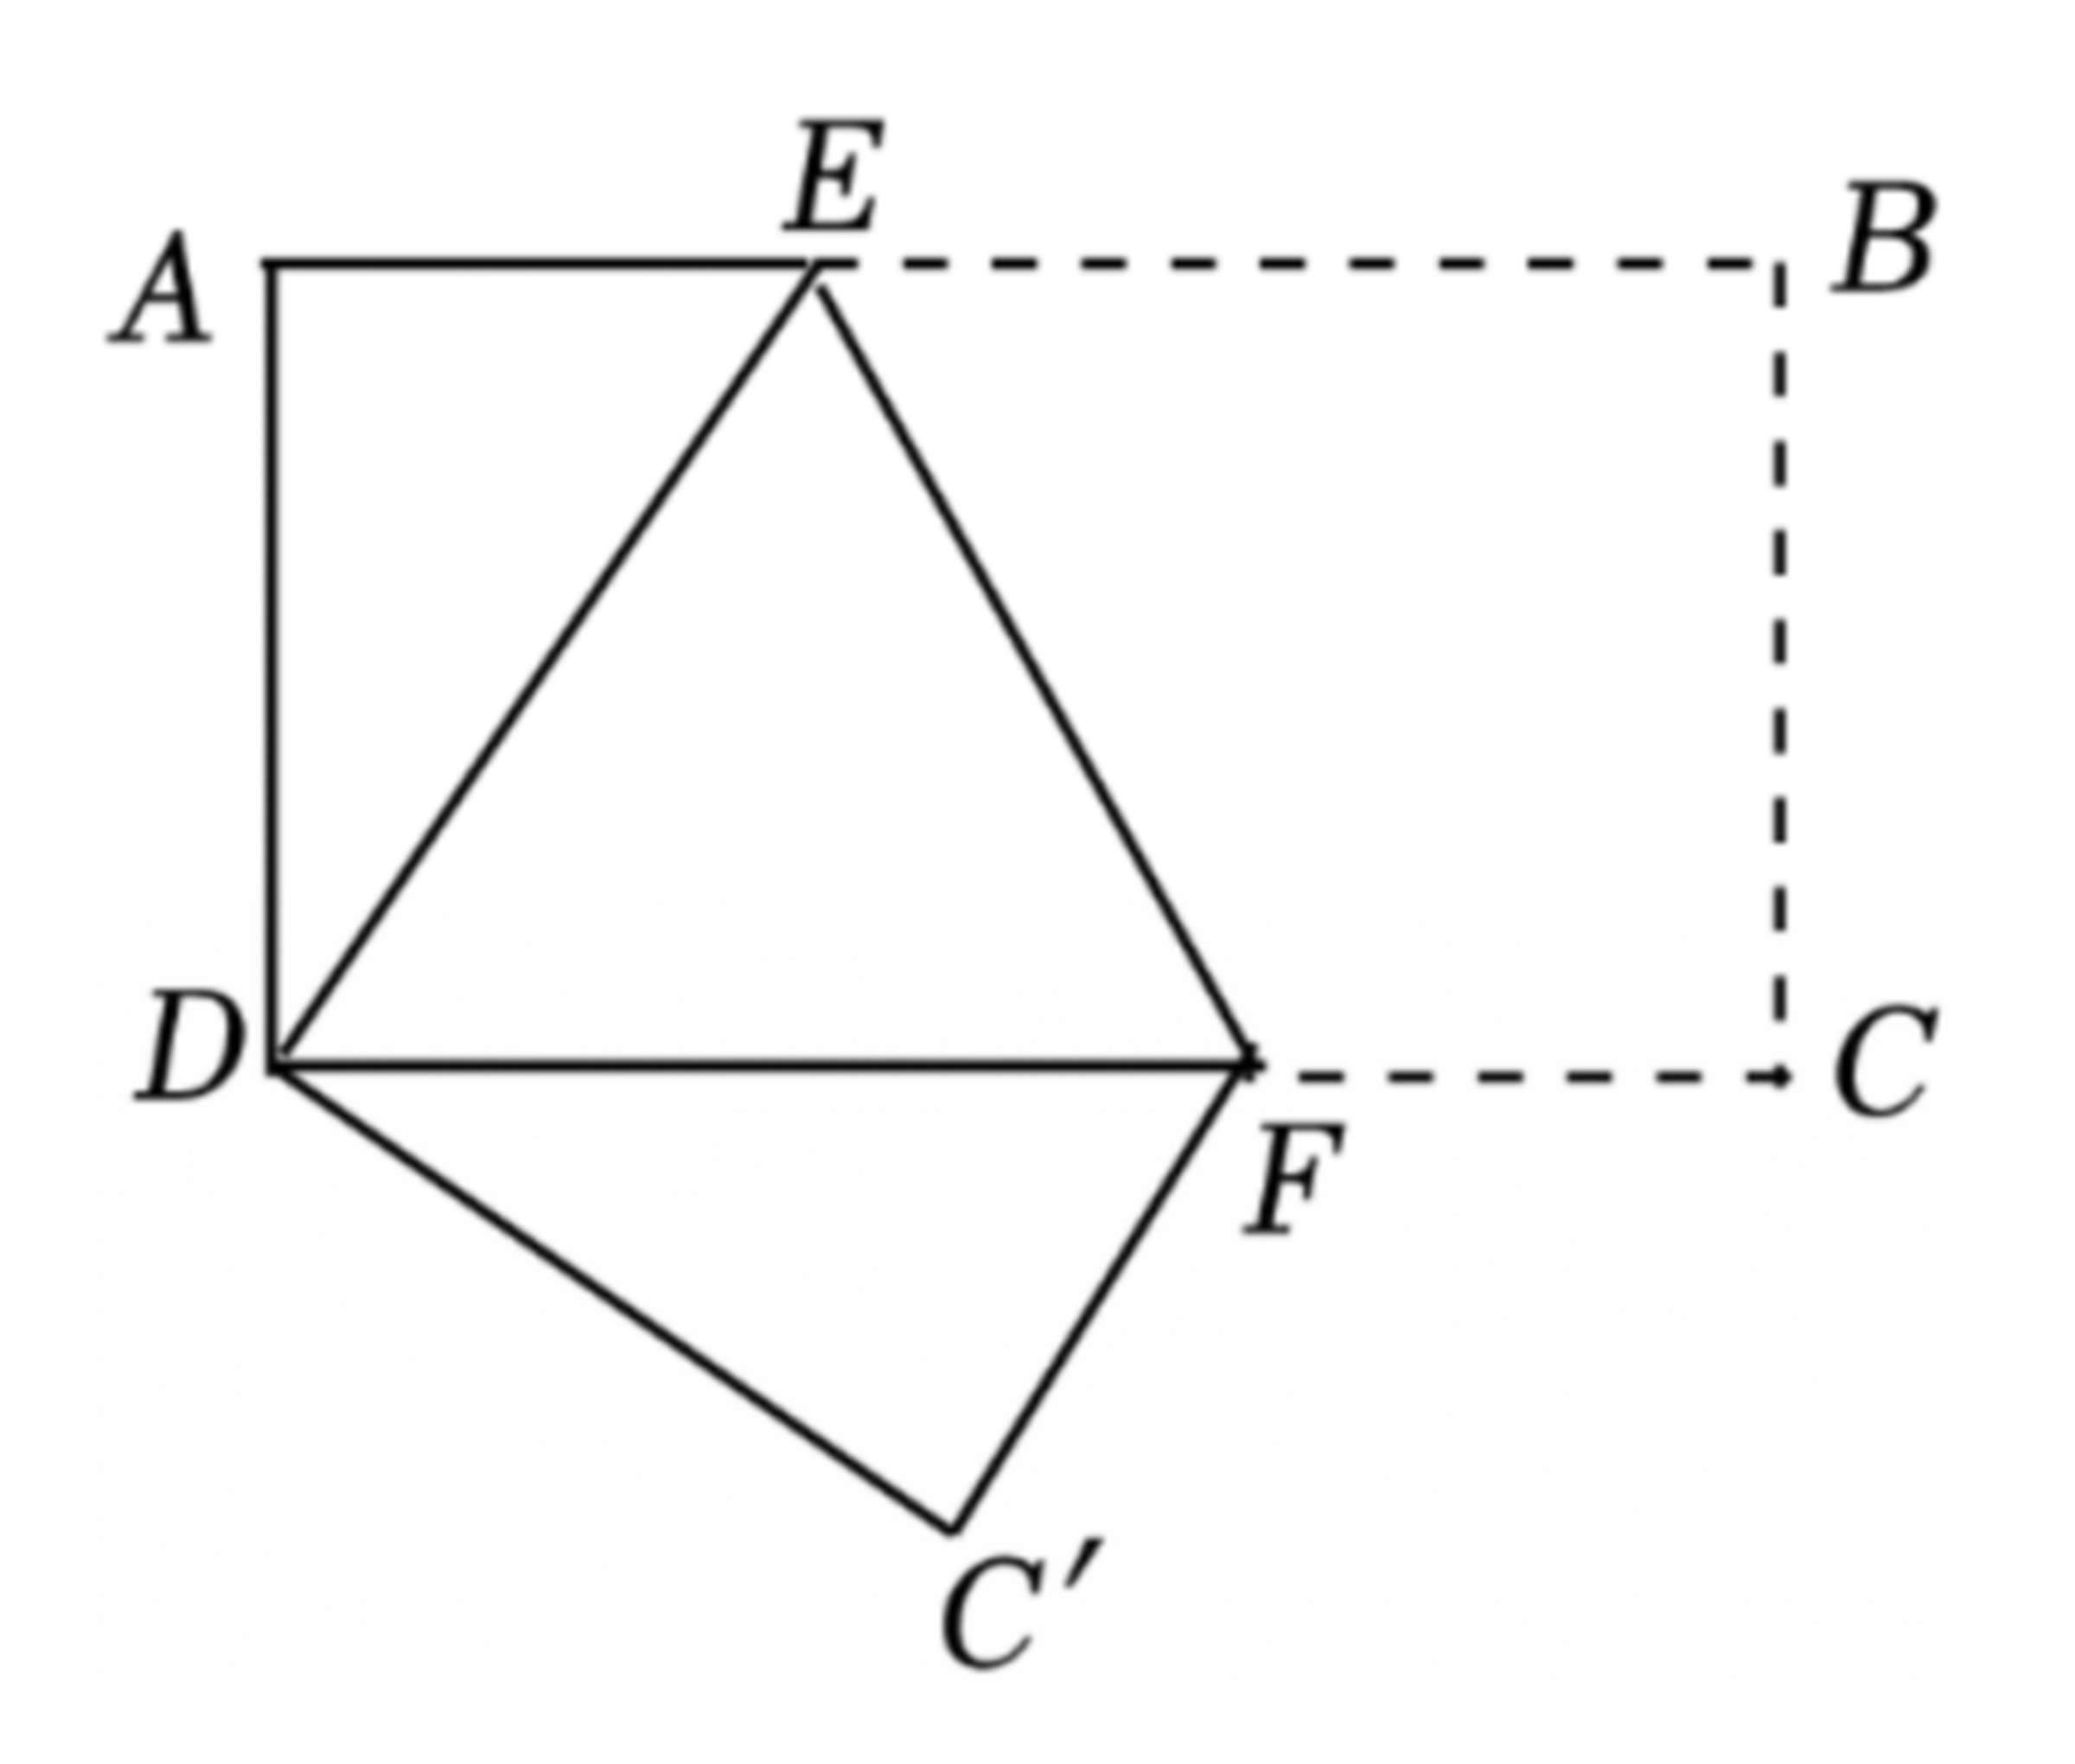
\includegraphics[width=0.40\textwidth]{figures/gao149_q11.png}
\end{center}

\ifanswer
\solbegin
\step{因为矩形 $ABCD(AB>AD)$ 的周长为 12，}
\step{在 $AB$ 和 $CD$ 边上分别取点 $E$ 和 $F$，将四边形 $BCFE$ 沿 $EF$ 折叠，}
\step{使点 $B$ 与点 $D$ 重合，此时点 $C$ 的对应点为 $C'$，}
\step{所以设 $AD=a$，$AB=b$，则 $2(a+b)=12$，}
\step{所以 $a+b=6$，且 $AB>AD$，所以 $b>a>0$，}
\step{设 $DF=x$，则 $C'F=b-x$，在 $Rt\triangle DC'F$ 中，$DC'=BC=a$，}% 几何三角形符号原卷印扁等边细线三角 $\triangle$，照录（放大 02 页确认）；$Rt$ 照录
\step{所以 $a^2+(b-x)^2=x^2$，解得 $x=\dfrac{a^2+b^2}{2b}$，}
\step{因此 $\triangle C'DF$ 的面积 $S=\dfrac{1}{2}\cdot DC'\cdot C'F=\dfrac{1}{2}\cdot a\cdot(b-x)$，}
\step{又 $b-x=b-\dfrac{(6-b)^2+b^2}{2b}=\dfrac{6(b-3)}{b}$，}
\step{所以 $S=\dfrac{1}{2}\cdot a\cdot\dfrac{6(b-3)}{b}=\dfrac{1}{2}\cdot(6-b)\cdot\dfrac{6(b-3)}{b}=\dfrac{3(6-b)(b-3)}{b}$}
\step{$=3\cdot\left(-b-\dfrac{18}{b}+9\right)$，又 $b+\dfrac{18}{b}\geqslant2\sqrt{b\cdot\dfrac{18}{b}}=6\sqrt{2}$，}
\step{当且仅当 $b=\dfrac{18}{b}$ 即 $b=3\sqrt{2}$ 时取等号，此时满足 $b>a$，}
\step{所以 $S\leqslant3\cdot(-6\sqrt{2}+9)=27-18\sqrt{2}$，故 $\triangle C'DF$ 面积的最大值为 $27-18\sqrt{2}$.}
\solend
\fi

% === Q12 === 解析内 3 幅三次函数曲线坐标图（仅答案版出）；解析 15 行（8 行 03 页＋7 行 04 页）
\item 已知 $m>0$，若存在 $t\in\R$，使得对任意 $x\in[0,m]$，不等式 $[(x-1)^2-t](x-t)\leqslant0$ 恒成立，则 $m$ 的最大值是\blankline[4.4em].

\ifanswer
\solbegin
\step{当 $t\leqslant0$ 时，$(x-1)^2-t\geqslant0$ 恒成立，}
\step{不等式 $[(x-1)^2-t](x-t)\leqslant0$ 的解集为 $x\leqslant t$，与 $x\in[0,m]$ 矛盾；}
\step{当 $t>0$ 时，不等式 $[(x-1)^2-t](x-t)\leqslant0\Leftrightarrow(x-1-\sqrt t)(x-1+\sqrt t)(x-t)\leqslant0$，}
\step{若 $t<1-\sqrt t$，即 $t\in\left(0,\dfrac{3-\sqrt5}{2}\right)$，}
\begin{center}
% 情形一 $t<1-\sqrt t$ 曲线图取 03 页右侧，去粉色水印、去色、4× LANCZOS 放大；仅答案版出
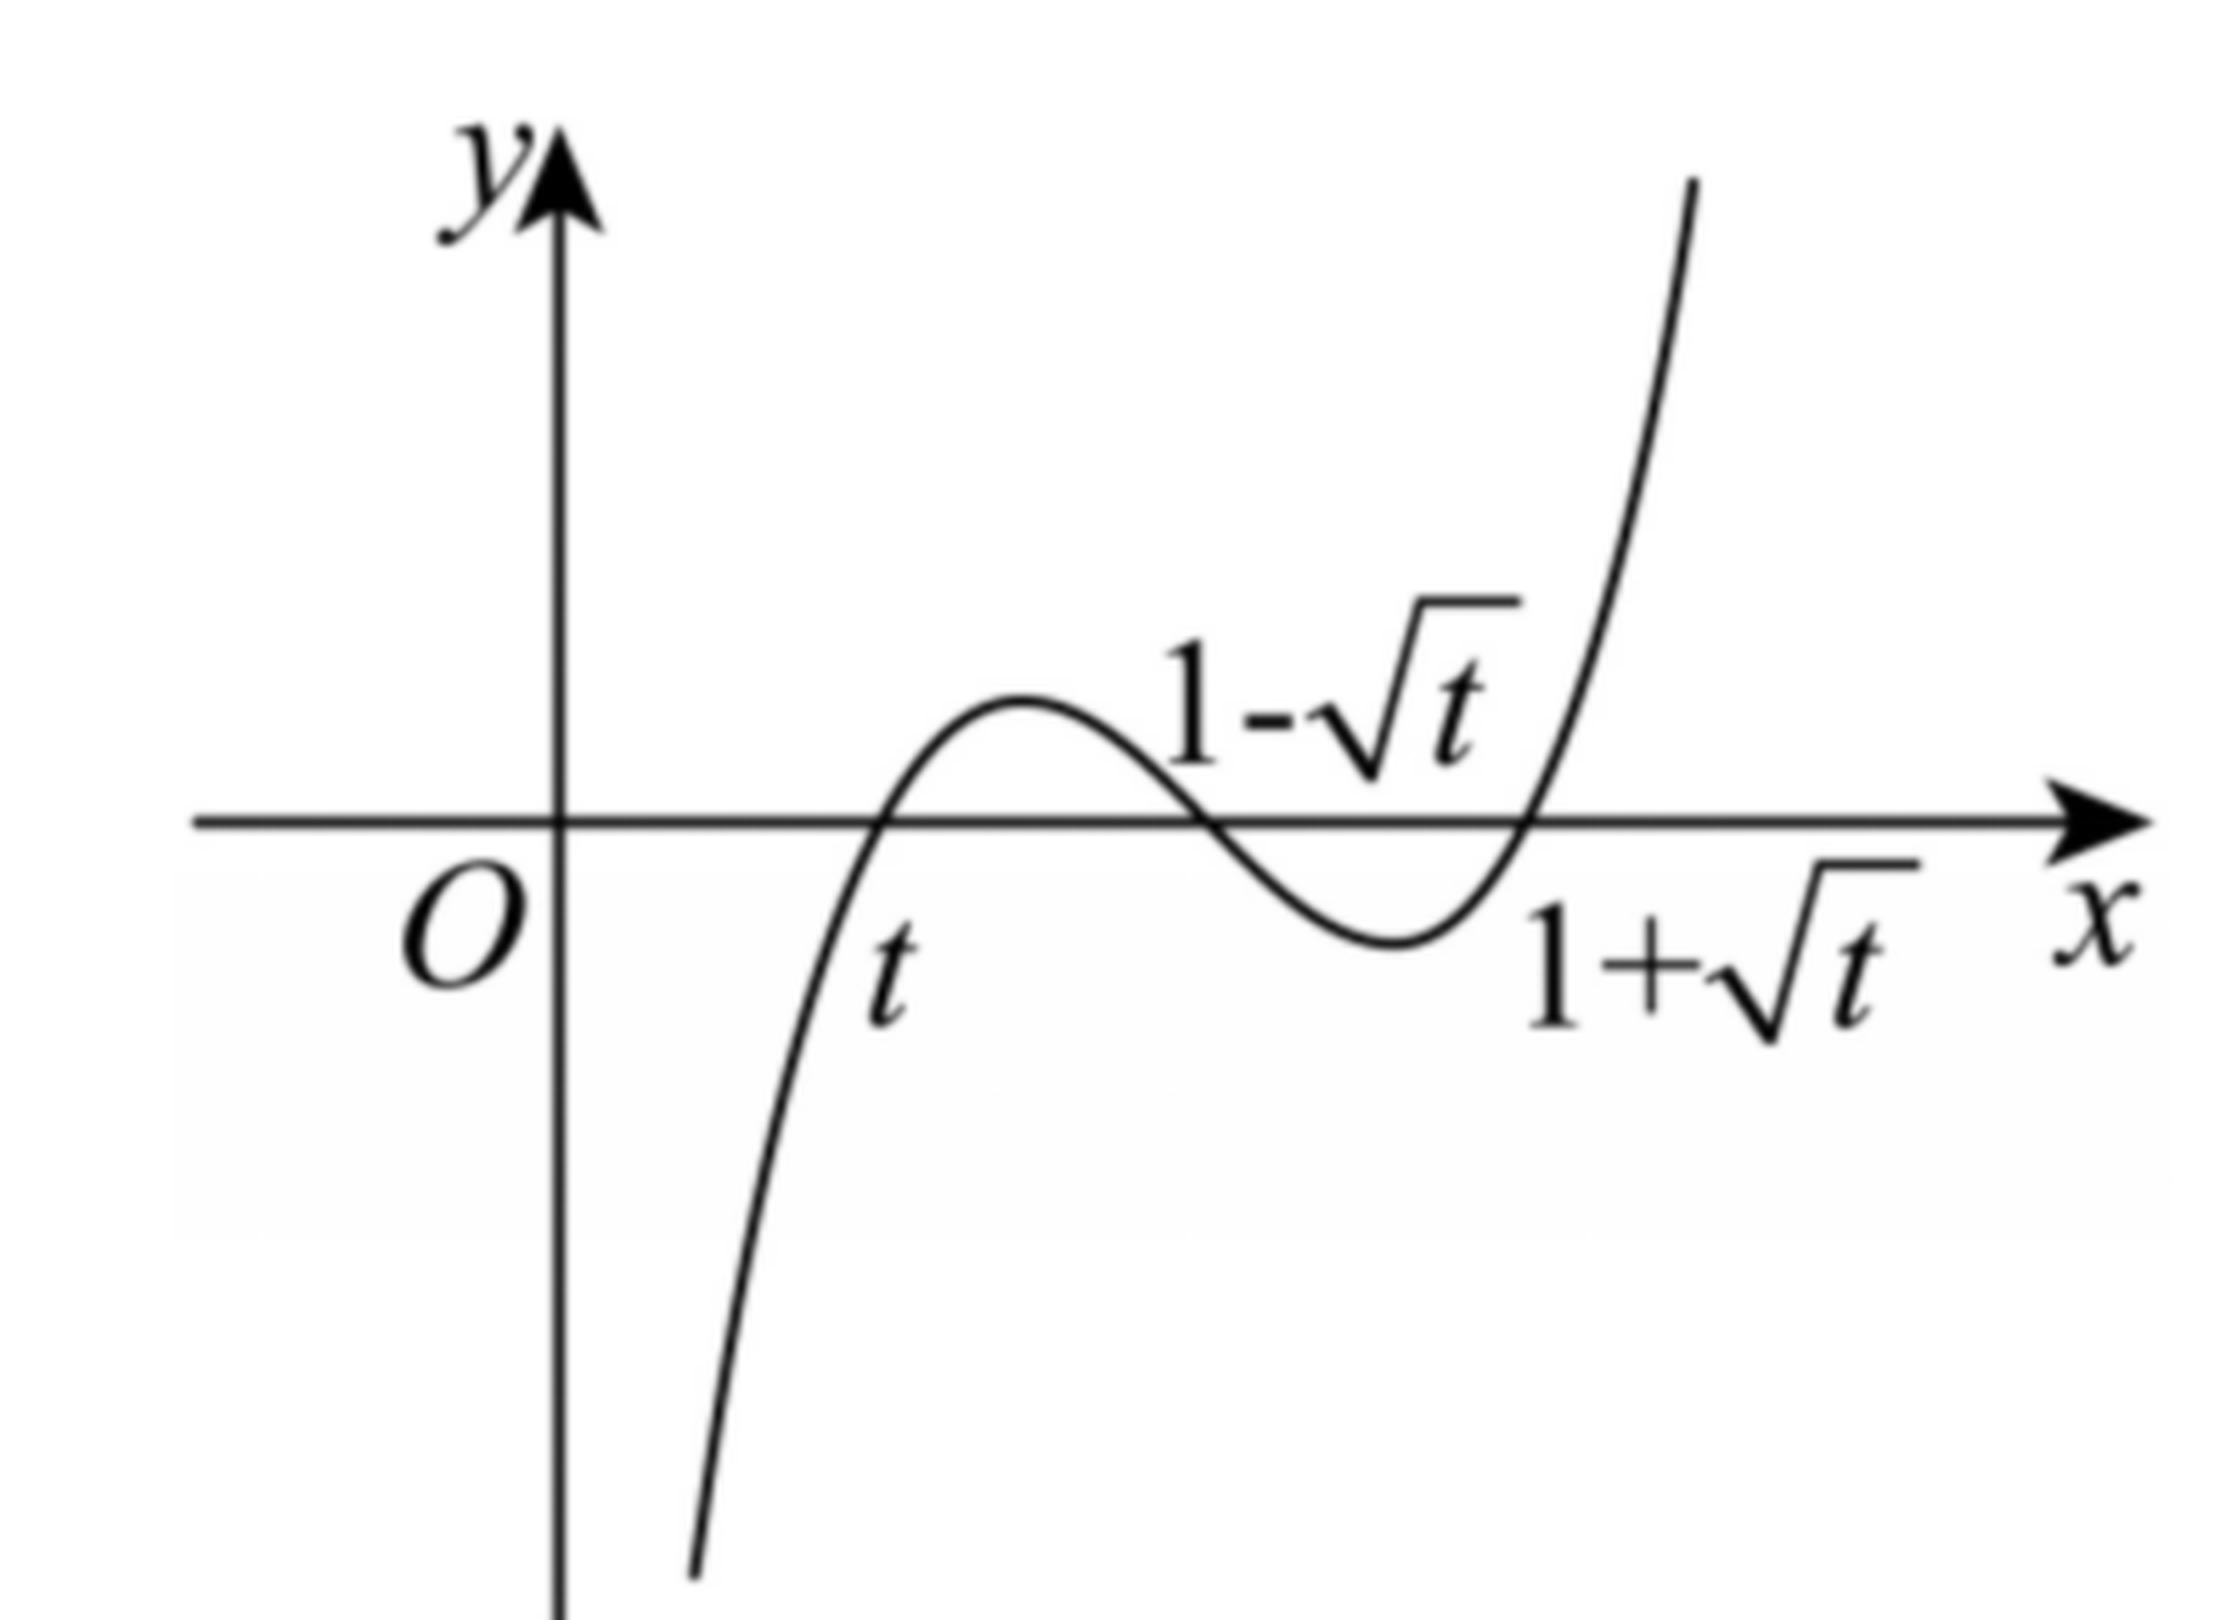
\includegraphics[width=0.40\textwidth]{figures/gao149_q12_a.png}
\end{center}
\step{则原不等式的解集为 $(-\infty,t]\cup[1-\sqrt t,1+\sqrt t]$，}
\step{当 $0<m\leqslant t$ 时，原不等式恒成立，因此}
\step{$m\in\left(0,\dfrac{3-\sqrt5}{2}\right)$；}
\step{若 $t=1-\sqrt t$，即 $t=\dfrac{3-\sqrt5}{2}$，则原不等式的解集为 $(-\infty,1+\sqrt t]$，}
\begin{center}
% 情形二 $t=1-\sqrt t$ 曲线图取 03 页右侧，去粉色水印、去色、4× LANCZOS 放大；仅答案版出
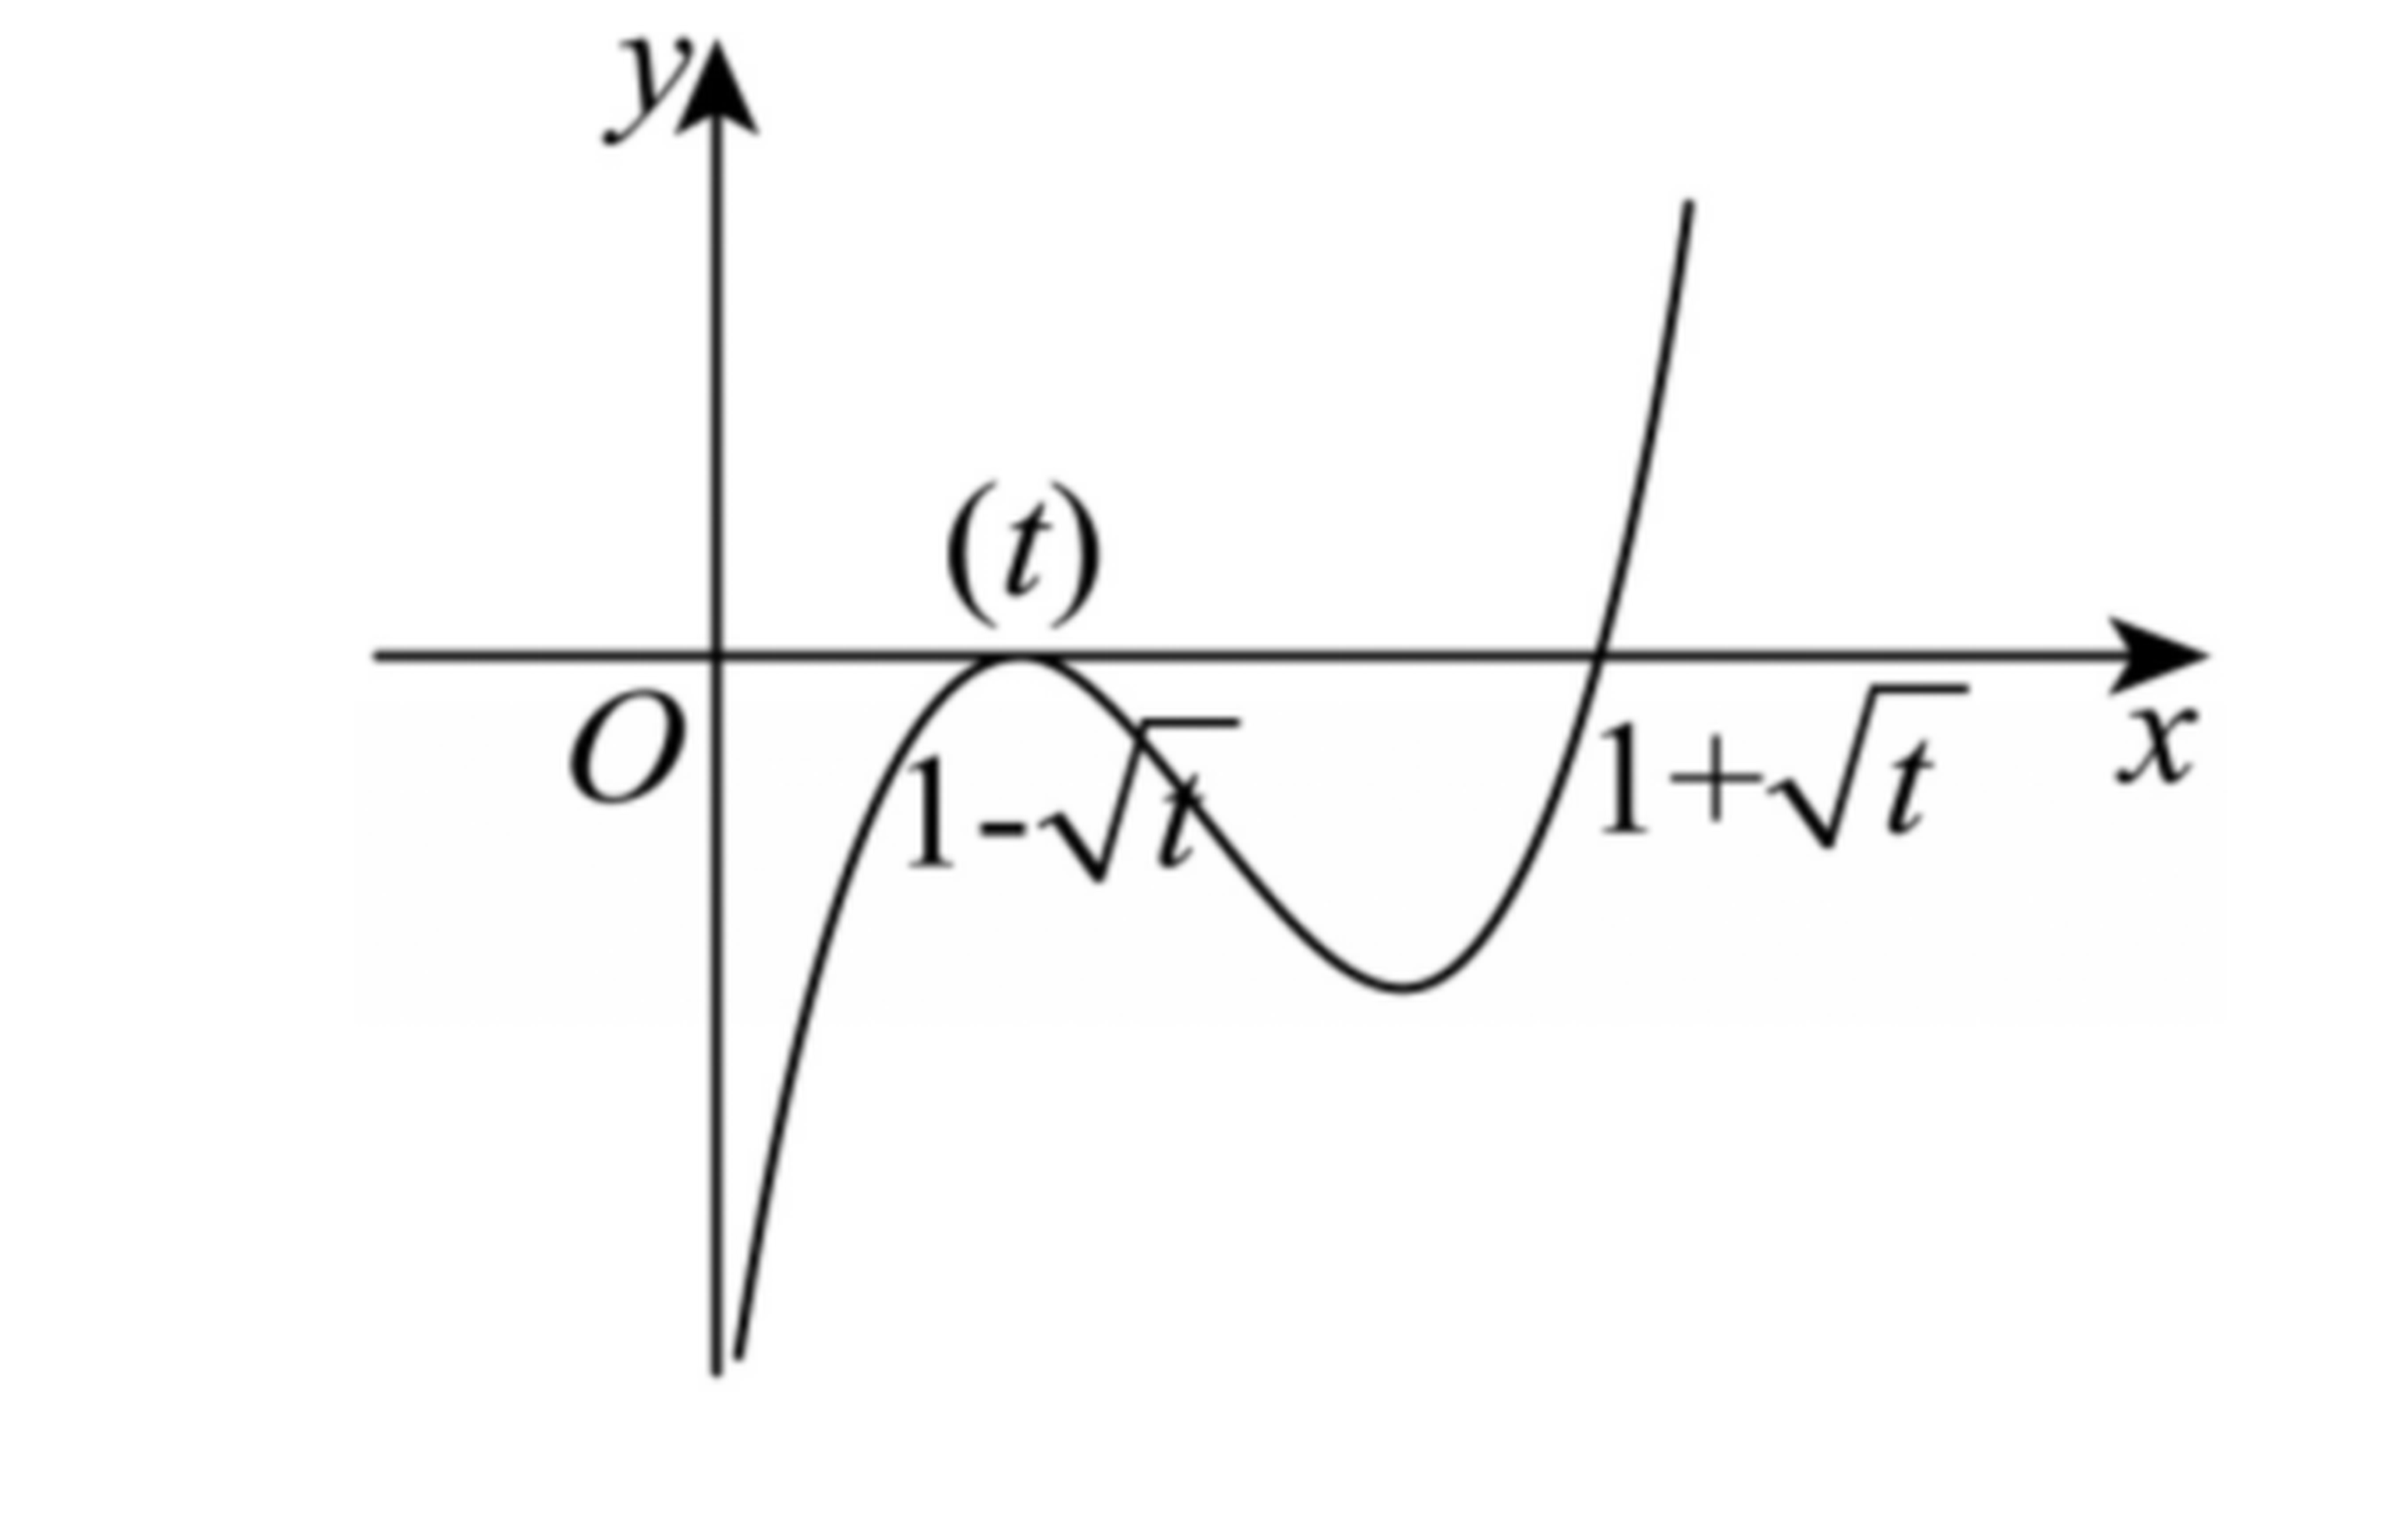
\includegraphics[width=0.40\textwidth]{figures/gao149_q12_b.png}
\end{center}
\step{当 $0<m\leqslant1+\sqrt t$ 时，原不等式恒成立，因此 $m\in\left(0,\dfrac{\sqrt5+1}{2}\right]$；}
\step{若 $1+\sqrt t>t>1-\sqrt t$，即 $t\in\left(\dfrac{3-\sqrt5}{2},\dfrac{3+\sqrt5}{2}\right)$，}
\begin{center}
% 情形三 $1+\sqrt t>t>1-\sqrt t$ 曲线图取 04 页右侧，去粉色水印、去色、4× LANCZOS 放大；仅答案版出
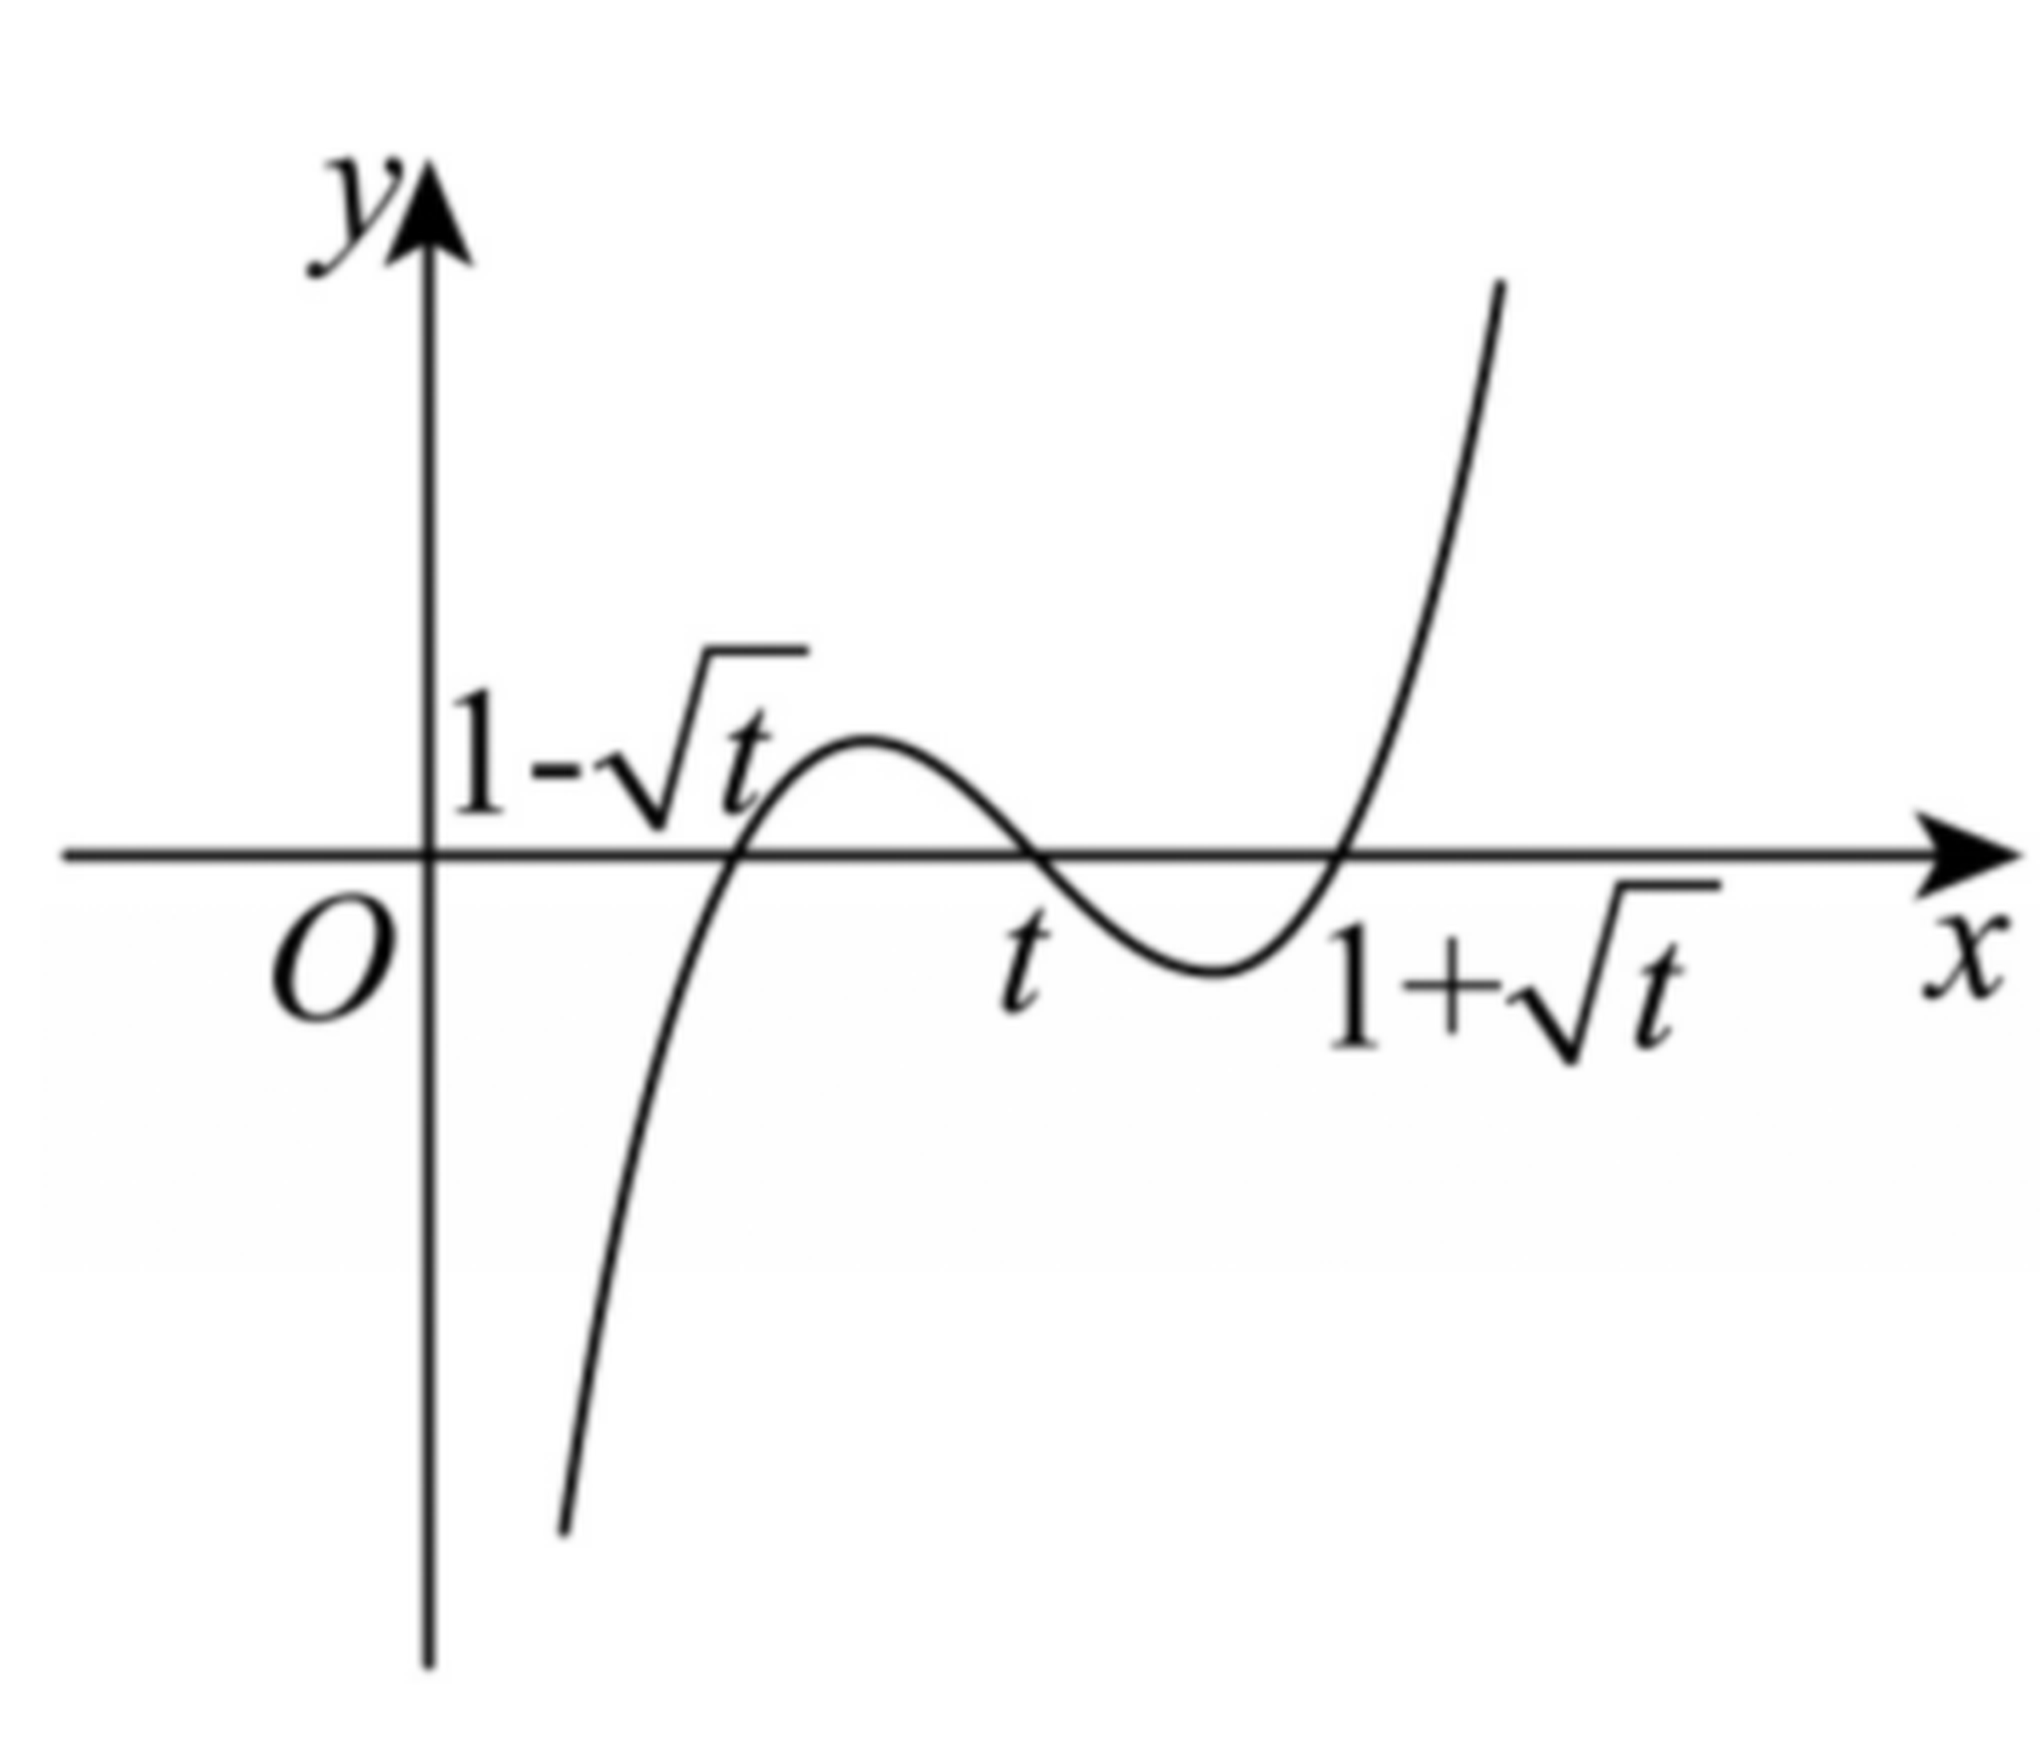
\includegraphics[width=0.40\textwidth]{figures/gao149_q12_c.png}
\end{center}
\step{则原不等式的解集为 $(-\infty,1-\sqrt t]\cup[t,1+\sqrt t]$，}
\step{当 $\begin{cases}1-\sqrt t>0\\1-\sqrt t\geqslant m\end{cases}$ 时，原不等式恒成立，此时 $t\in\left(\dfrac{3-\sqrt5}{2},1\right)$，$m\in\left(0,\dfrac{3-\sqrt5}{2}\right)$；}
\step{若 $t\geqslant1+\sqrt t$，即 $t\geqslant\dfrac{3+\sqrt5}{2}$，则取 $x=0$，$(t-1)t>0$，}
\step{原不等式不恒成立，不符合题意，}
\step{因此实数 $m$ 的取值范围是 $\left(0,\dfrac{\sqrt5+1}{2}\right]$，$m$ 的最大值是 $\dfrac{\sqrt5+1}{2}$.}
\solend
\fi

\end{enumerate}

\bigsec{二、选择题}

\begin{enumerate}
\setcounter{enumi}{12}

% === Q13 ===：答案"C"直接印在题干括号内、无【答案】/【解析】段，按 高一84 Q13／高一148 Q13 成例括号留空、另提 \ans{$C$}；四选项两行两列照原卷分行
\item 设 $ab>0$，则 $a>b$ 是 $\dfrac{1}{a}<\dfrac{1}{b}$ 的\mbox{（\quad）}

\keepwithprev
A. 充分不必要条件\qquad\qquad B. 必要不充分条件

C. 充要条件\qquad\qquad D. 既不充分又不必要条件

\ifanswer
\ans{$C$}
\fi

% === Q14 ===：$A\subset B$ 单线照录；四选项补集照原卷上划线 \overline{A}／\overline{B}；解析 1 行（由韦恩图得 B 对）
\item 已知集合 $A$、$B$ 非空，且 $A\subset B$，则下列式子中一定是空集的为\mbox{（\quad）}

\keepwithprev
A. $\overline{A}\cap B$\qquad B. $A\cap\overline{B}$\qquad C. $\overline{A}\cap\overline{B}$\qquad D. $\overline{A}\cup\overline{B}$

\ifanswer
\solbegin
\step{由韦恩图得 $B$ 对. 故选 $B$.}
\solend
\fi

% === Q15 ===："天文数字"弯引号照录；解析 2 行（首行在 04 页末、末行续 05 页顶）
\item 历史上数学计算方面的三大发明是阿拉伯数字、十进制和对数，其中对数的发明，大大缩短了计算时间，为人类研究科学和了解自然起了重大作用，对数运算对估算“天文数字”具有独特的优势. $2.5^{1000}$ 的估算值约为\mbox{（\quad）}

\keepwithprev
A. $10^{365}$\qquad B. $10^{379}$\qquad C. $10^{389}$\qquad D. $10^{398}$

\ifanswer
\solbegin
\step{$\lg 2.5^{1000}=1000\lg 2.5=1000(1-2\lg 2)\approx1000\times(1-0.602)=398$，}
\step{所以 $2.5^{1000}\approx10^{398}$. 故选 $D$.}
\solend
\fi

% === Q16 ===："完美集"新定义、圈数字①②文本模式；题干"若对任意 $x$，$y\in A$"用全角逗号、解析用顿号"$x$、$y\in A$"，两处照录不统一；解析 9 行
\item 设全集 $U=\R$，集合 $A$ 是一个非空数集，若对任意 $x$，$y\in A$，都有 $x+y\in A$、$xy\in A$，则称集合 $A$ 为一个“完美集”，给出以下命题：

①若 $A_1$、$A_2$ 都是“完美集”，且 $A_1\cap A_2\ne\varnothing$，则 $A_1\cap A_2$ 也是“完美集”；

②若 $A_1$、$A_2$ 都是“完美集”，则 $A_1\cup A_2$ 也是“完美集”.

下列说法正确的是\mbox{（\quad）}

\keepwithprev
A. ①②都是真命题\qquad\qquad B. ①是真命题，②是假命题

C. ①是假命题，②是真命题\qquad\qquad D. ①②都是假命题

\ifanswer
\solbegin
\step{由题意，全集 $U=\R$，集合 $A$ 是一个非空数集，}
\step{若对任意 $x$、$y\in A$，都有 $x+y\in A$、$xy\in A$，则称集合 $A$ 为一个“完美集”，}
\step{对于①，取 $x$、$y\in A_1\cap A_2$，则 $x\in A_1$，$x\in A_2$，$y\in A_1$，$y\in A_2$，}
\step{又 $A_1$、$A_2$ 是“完美集”，所以 $x+y\in A_1$，$xy\in A_1$，$x+y\in A_2$，$xy\in A_2$，}
\step{所以 $x+y\in A_1\cap A_2$，$xy\in A_1\cap A_2$，所以 $A_1\cap A_2$ 是“完美集”，故①正确；}
\step{对于②，取“完美集” $A_1=\{x\mid x=2k,k\in\Z\}$，$A_2=\{x\mid x=3k,k\in\Z\}$，}
\step{则 $2\in A_1$，$3\in A_2$，但 $2+3\notin A_1\cup A_2$，}
\step{即此时 $A_1\cup A_2$ 不是“完美集”，故②错误.}
\step{故选 $B$.}
\solend
\fi
\end{enumerate}

\bigsec{三、解答题}

\begin{enumerate}
\setcounter{enumi}{16}

% === Q17 ===："图像"（有亻）照录（Q17 题干与解析共 2 处）；绝对值 \lvert…\rvert；解析 7 行
\item 已知 $m\in\R$，$f(x)=(m^2-m-5)x^m$. 若 $y=f(x)$ 是幂函数，且其图像不经过原点.

(1) 求实数 $m$ 的值；

(2) 若 $f(a)=f(b)$ 且 $a\ne b$，求 $\lvert a+2\rvert+\lvert b-1\rvert$ 的最小值，并指出取到最小值时 $a$ 的取值范围.

\ifanswer
\solbegin
\step{(1) $f(x)=(m^2-m-5)x^m$ 是幂函数，得 $m^2-m-5=1$，即 $m^2-m-6=0$，}
\step{解得 $m=-2$ 或 $m=3$，又函数图像不经过原点，所以 $m=-2$($3$ 舍)；}
\step{(2) 由 (1) 得 $f(x)=x^{-2}=\dfrac{1}{x^2}$ 为偶函数，}
\step{$x<0$ 时，函数 $f(x)$ 严格增，$x>0$ 时，函数 $f(x)$ 严格减，}
\step{又 $f(a)=f(b)$ 且 $a\ne b$，所以 $a=-b$，且 $a\ne0$，$b\ne0$，}
\step{则 $\lvert a+2\rvert+\lvert b-1\rvert=\lvert a+2\rvert+\lvert-a-1\rvert=\lvert a+2\rvert+\lvert a+1\rvert$，}
\step{则 $\lvert a+2\rvert+\lvert b-1\rvert$ 的最小值为 $1$，取到最小值时 $a$ 的取值范围是 $[-2,-1]$.}
\solend
\fi

% === Q18 ===：判别式两形混用——(1) cases 块印高 \Delta、(2) 独立行印扁 \triangle，逐处照录不统一；解析 8 行
\item 已知命题 $p$：方程 $x^2+4x+m-1=0$ 有两个不等的负根；命题 $q$：方程 $4x^2+4x+m-2=0$ 无实根.

(1) 若 $p$ 为真命题，求 $m$ 的取值范围；

(2) 若 $p$、$q$ 两命题一真一假，求 $m$ 的取值范围.

\ifanswer
\solbegin
\step{(1) 若 $p$ 为真命题，即方程 $x^2+4x+m-1=0$ 有两个不等的负根；}
\step{必有 $\begin{cases}\Delta=16-4(m-1)>0\\m-1>0\end{cases}$，解得 $1<m<5$，即 $m$ 的取值范围为 $(1,5)$；}
\step{(2) 命题 $q$：方程 $4x^2+4x+m-2=0$ 无实根，}
\step{则有 $\triangle=16-16(m-2)<0$，解得 $m>3$，}
\step{若 $p$ 和 $q$ 有且只有一个为真命题，}
\step{若 $p$ 真 $q$ 假，必有 $\begin{cases}1<m<5\\m\leqslant3\end{cases}$，则有 $1<m\leqslant3$，}
\step{若 $p$ 假 $q$ 真，必有 $\begin{cases}m\leqslant1\text{ 或 }m\geqslant5\\m>3\end{cases}$，则有 $m\geqslant5$，}
\step{综上，$1<m\leqslant3$ 或 $m\geqslant5$.}
\solend
\fi

% === Q19 ===：$A\subseteq B$ 带下划线照录；解析 7 行（(2) 两组 cases 并排）
\item 已知 $m\in\R$，集合 $A=\left\{x\mid y=\sqrt{3-x}-\dfrac{1}{\sqrt{x-1}}\right\}$，集合 $B=\{x\mid 2m\leqslant x\leqslant1-m\}$.

(1) 若 $A\cup B=B$，求实数 $m$ 的取值范围；

(2) 若 $A\cap B=\varnothing$，求实数 $m$ 的取值范围.

\ifanswer
\solbegin
\step{(1) 函数 $y=\sqrt{3-x}-\dfrac{1}{\sqrt{x-1}}$，则 $\begin{cases}3-x\geqslant0\\x-1>0\end{cases}$，解得 $1<x\leqslant3$，}
\step{所以 $A=\{x\mid1<x\leqslant3\}$，}
\step{因为 $A\cup B=B$，所以 $A\subseteq B$，则 $\begin{cases}2m\leqslant1\\1-m\geqslant3\end{cases}$，解得 $m\leqslant-2$，}
\step{综上，实数 $m$ 的取值范围为 $(-\infty,-2]$；}
\step{(2) 当 $B=\varnothing$ 时，则 $2m>1-m$，解得 $m>\dfrac{1}{3}$，}
\step{当 $B\ne\varnothing$ 时，则 $\begin{cases}2m\leqslant1-m\\2m>3\end{cases}$ 或 $\begin{cases}2m\leqslant1-m\\1-m\leqslant1\end{cases}$，解得 $m\in\varnothing$ 或 $0\leqslant m\leqslant\dfrac{1}{3}$，}
\step{综上，实数 $m$ 的取值范围为 $[0,+\infty)$.}
\solend
\fi

% === Q20 ===：n 阶基本不等式推广；(3) 解析含 \overbrace{…}^{k} 上括号；(2) 解析"x=x=x=3(1-x)"三连等系原卷笔误、照录加注（见 ⑤）；解析 14 行
\item 教材中的基本不等式可以推广到 $n$ 阶：$n$ 个正数的算术平均数不小于它们的几何平均数，即对于任意的正数 $a_1$、$a_2$、$\cdots$、$a_n$，有 $\dfrac{a_1+a_2+\cdots+a_n}{n}\geqslant\sqrt[n]{a_1\cdot a_2\cdots a_n}$（$n\in\N$ 且 $n\geqslant2$），且等号当且仅当 $a_1=a_2=\cdots=a_n$ 时成立. 利用此结论解决下列问题：

(1) 若 $x$、$y$、$z>0$，求 $\dfrac{y}{x}+\dfrac{2z}{y}+\dfrac{4x}{z}$ 的最小值；

(2) 已知 $0<x<1$，求 $x^3(1-x)$ 的最大值，并求取得最大值时的 $x$ 的值；

(3) 对任意的正整数 $k$，判断 $\left(1+\dfrac{1}{k}\right)^k$ 与 $\left(1+\dfrac{1}{k+1}\right)^{k+1}$ 的大小关系，并证明.

\ifanswer
\solbegin
\step{(1) 因为 $x$、$y$、$z>0$，有 $\dfrac{y}{x}>0$，$\dfrac{2z}{y}>0$，$\dfrac{4x}{z}>0$}
\step{所以 $\dfrac{y}{x}+\dfrac{2z}{y}+\dfrac{4x}{z}\geqslant3\sqrt[3]{\dfrac{y}{x}\cdot\dfrac{2z}{y}\cdot\dfrac{4x}{z}}=3\sqrt[3]{8}=6$，}
\step{当且仅当 $\dfrac{y}{x}=\dfrac{2z}{y}=\dfrac{4x}{z}$ 时取等号，故 $\dfrac{y}{x}+\dfrac{2z}{y}+\dfrac{4x}{z}$ 的最小值为 $6$.}
\step{(2) 因为 $0<x<1$，所以 $1-x>0$，}
\step{$x^3(1-x)=\dfrac{1}{3}[x\cdot x\cdot x\cdot3(1-x)]\leqslant\dfrac{1}{3}\left[\dfrac{x+x+x+3(1-x)}{4}\right]^4=\dfrac{1}{3}\times\left(\dfrac{3}{4}\right)^4$}
\step{$=\dfrac{27}{256}$，当且仅当 $x=x=x=3(1-x)$，即 $x=3(1-x)$，$x=\dfrac{3}{4}$ 取等号，}% 原卷"x=x=x=3(1-x)"三连等，疑为四因子相等之误排，放大 08 页确认，照录未改（见 ⑤）
\step{所以 $0<x<1$ 时，$x^3(1-x)$ 的最大值是 $\dfrac{27}{256}$，取最大值时 $x=\dfrac{3}{4}$.}
\step{(3) 对任意 $k\in\N^*$，$\left(1+\dfrac{1}{k}\right)^k<\left(1+\dfrac{1}{k+1}\right)^{k+1}$.}
\step{证明：$\left(1+\dfrac{1}{k}\right)^k=\overbrace{\left(1+\dfrac{1}{k}\right)\cdot\left(1+\dfrac{1}{k}\right)\cdots\left(1+\dfrac{1}{k}\right)}^{k}\times1$}
\step{$\leqslant\left(\dfrac{\overbrace{\left(1+\dfrac{1}{k}\right)+\left(1+\dfrac{1}{k}\right)+\cdots+\left(1+\dfrac{1}{k}\right)}^{k}+1}{k+1}\right)^{k+1}$}
\step{$=\left(\dfrac{\overbrace{(1+1+\cdots+1)}^{k}+\overbrace{\left(\dfrac{1}{k}+\dfrac{1}{k}+\cdots+\dfrac{1}{k}\right)}^{k}+1}{k+1}\right)^{k+1}=\left(\dfrac{k+1+1}{k+1}\right)^{k+1}=\left(1+\dfrac{1}{k+1}\right)^{k+1}$，}
\step{当且仅当 $1+\dfrac{1}{k}=1$ 时取等号，}
\step{但是任意 $k\in\N^*$ 时 $1+\dfrac{1}{k}>1$，所以等号不成立，}
\step{故任意 $k\in\N^*$ 时，$\left(1+\dfrac{1}{k}\right)^k<\left(1+\dfrac{1}{k+1}\right)^{k+1}$.}
\solend
\fi

% === Q21 ===："减 k 集"新定义（引号内 k／数字两侧空格照录）；解析 26 行（续 10 页），含 ⑤ 三处原卷笔误照录
\item 定义：对于给定的整数 $k$，若非空集合 $A$ 满足如下 3 个条件：

① $A$ 是正整数集的子集；② $A\ne\{1\}$；

③对任意正整数 $x,y$，若 $x+y\in A$，则 $xy-k\in A$；则称集合 $A$ 为“减 $k$ 集”.

(1) 判断集合 $A=\{1,2\}$ 是否为“减 $0$ 集”？是否为“减 $1$ 集”？（无需说明理由）

(2) 证明：不存在“减 $2$ 集”；

(3) 是否存在“减 $1$ 集”？如果存在，求出所有“减 $1$ 集”；如果不存在，说明理由.

\ifanswer
\solbegin
\step{(1) 因为 $P\subseteq\N^*$，$P\ne\{1\}$，$1+1=2\in P$，$1\times1-0\in P$，}
\step{所以集合 $P=\{1,2\}$ 是“减 $0$ 集”；}
\step{因为 $P\subseteq\N^*$，$P\ne\{1\}$，$1+1=2\in P$，$1\times1-1\notin P$，}
\step{所以集合 $P=\{1,2\}$ 是“减 $1$ 集”；}% 按条件③应为"不是"，原卷径印"是"，放大 09 页确认，照录未改（见 ⑤）
\step{(2) 假设存在集合 $A$ 是“减 $2$ 集”，若 $x+y\in A$，则 $xy-2\in A$，}
\step{①当 $x+y=xy-2$ 时，有 $(x-1)(y-1)=3$，}
\step{则 $x$、$y$ 一个为 $2$，一个为 $4$，所以集合 $A$ 有元素 $6$，}
\step{但 $3+3\in A$，$3\times3-2\notin A$，与 $A$ 是“减 $2$ 集”矛盾；}
\step{②当 $x+y\ne xy-2$ 时，则 $x+y=xy-1$ 或 $x+y=xy-m$($m>2$)，}
\step{若 $x+y=xy-1$，$m=1$ 时，$M$ 为除 $1$ 以外的最小元素，}% 原卷"m=1"上文未显式定义，疑笔误，放大 09 页确认，照录未改（见 ⑤）
\step{则 $x=M-1$，$y=1$ 时，$xy-2=M-3$ 小于 $M$，}
\step{要符合题意，必须 $M=4$，}
\step{此时取 $x-2$，$y=2$，$xy-2=2$ 不属于 $A$，故不符合题意，}% 原卷"取 x−2"疑为"取 x=2"误排，放大 09 页确认，照录未改（见 ⑤）
\step{当 $m>2$ 时，$(x-1)(y-1)=m+1$，同样得出矛盾，}
\step{综上，不存在 $A$ 是“减 $2$ 集”.}
\step{(3) 存在“减 $1$ 集” $A$，则 $A\ne\{1\}$，}
\step{①假设 $1\in A$，则 $A$ 中除了元素 $1$ 以外，必然还含有其它元素，}
\step{假设 $2\in A$，$1+1\in A$，而 $1\times1-1\notin A$，所以 $2\notin A$，}
\step{假设 $3\in A$，$1+2\in A$，而 $1\times2-1\in A$，所以 $3\in A$，}
\step{所以 $A=\{1,3\}$，}
\step{假设 $4\in A$，$1+3\in A$，而 $1\times3-1\notin A$，所以 $4\notin A$，}
\step{假设 $5\in A$，$1+4\in A$，$1\times4-1\in A$，$2+3=5$，$2\times3-1\in A$，所以 $5\in A$，}
\step{所以 $A=\{1,3,5\}$，}
\step{以此类推，得 $A=\{1,3,5,\cdots,2n-1,\cdots\}$，($n\in\N^*$)，}
\step{所以所有的“减 $1$ 集”有 $\{1,3\}$，$\{1,3,5\}$，$\{1,3,5,7\}$，$\cdots$，$\{1,3,5,\cdots,2n-1,\cdots\}$，}
\step{$(n\in\N^*)$.}
\solend
\fi
\end{enumerate}

\end{document}
"
% 紧凑版：xelatex "\def\iscompact{1}% 高一149_青浦高级中学上外云间_期中.tex
%   —— 高一上数学"2026-2027 年青浦高级中学上外云间高一上期中"（试卷版/答案版/紧凑版）
% 试卷版：xelatex 高一149_青浦高级中学上外云间_期中.tex
% 答案版：xelatex "\def\isanswer{1}% 高一149_青浦高级中学上外云间_期中.tex
%   —— 高一上数学"2026-2027 年青浦高级中学上外云间高一上期中"（试卷版/答案版/紧凑版）
% 试卷版：xelatex 高一149_青浦高级中学上外云间_期中.tex
% 答案版：xelatex "\def\isanswer{1}\input{高一149_青浦高级中学上外云间_期中.tex}"
% 紧凑版：xelatex "\def\iscompact{1}\input{高一149_青浦高级中学上外云间_期中.tex}"
%
% ① 原始材料：微信公众号"魔都数学加油站"文章，连载"27学年高一149"，原文标题
% "27学年高一149——2026-2027年上海市青浦高级中学上外云间高一上期中"；
% 原文链接：https://mp.weixin.qq.com/s/T7_nyoR1k0o_5og7FkDsyw 。
% 正文为 10 张 PNG 页（01/02/03/04/10 为 2560×3620，05/06/07/08/09 为 4762×6735，
% 同一篇各页分辨率混排，逐页按各自分辨率裁图核对，别按预览比例换算裁框）。
% 体例：混合体例讲评版——19 题中 Q6 只印【答案】、无【解析】；Q13 的答案"C"
%   直接印在题干括号内、无【答案】/【解析】段；其余 17 题印【解析】（逐题核实，见 ② ②）。
% 题目、答案、解析均据原图转录；卷面粉红色水印"魔都数学加油站"及公众号页脚未录入。
% 全卷插图清单（逐页通读 10 页确认）：1 幅题目配图 + 3 幅【解析】内配图：
%   · Q11 矩形 ABCD 折叠几何图（02 页右侧：A/B/C/D/E/F/C' 与虚线 EB、BC、FC），
%     题干"如图"处，题目配图、三版都出，裁 figures/gao149_q11.png；
%   · Q12【解析】内 3 幅三次函数曲线坐标图（03 页右侧两幅 + 04 页右侧一幅：
%     x/y 轴、O、t、1-\sqrt t、1+\sqrt t 等标注，分别对应 t<1-\sqrt t、
%     t=1-\sqrt t、1+\sqrt t>t>1-\sqrt t 三种情形），解析配图、仅答案版出，
%     分别裁 figures/gao149_q12_a.png／_b.png／_c.png，放 \ifanswer 内 \step 之间
%     （高一73 第 16 题成例）；
%   其余各页逐页确认无其它题目配图、无表格；Q14 解析"由韦恩图得 B 对"仅文字推导、
%   原卷并未印韦恩图；Q9／Q18／Q19 的 cases 块与 Q20(3) 的 \overbrace 为数学块（非图）；
%   10 页下半仅水印、无正文。4 图均取自原卷截图，去粉色水印、去色、4× LANCZOS 放大。
%
% 卷首标题：原卷印作"2026-2027 年青浦高级中学上外云间高一上期中"，年份区间按全稿
% 惯例排 en dash；原卷卷面未印副标题，本稿按同期中卷（高一140／141／143／144／145／
% 146／147／148）知识模块口径补出"集合与常用逻辑用语、不等式、函数"。
%
% 题号体例（逐页核实定稿）：本卷共 19 题——一、填空题 3—12（10 题）、
% 二、选择题 13—16（4 题）、三、解答题 17—21（5 题）。
% 三节分别 \setcounter{enumi}{2}／{12}／{16}。原卷从第 3 题起、无第 1、2 题，
% 本稿保留原题号；全卷无附加题节（Q21 解析末行"（n\in N^*）."为全卷收尾）。
%
% ② 与原卷的排版差异：
%   ① 原文从第 3 题起，本稿保留原题号；共 19 题三节；
%   ② 混合体例逐题核实：Q6（反证法"假设的内容"）只印【答案】、无【解析】，
%      按 高一140 第 5 题／高一145 Q3 成例提 \ans{}、不补造解析；Q13 答案"C"直接
%      印在题干括号内、全卷无该题【答案】/【解析】段，按 高一84 Q13／高一148 Q13
%      成例括号 \mbox{（\quad）} 留空、另提 \ans{$C$}；其余 17 题印【解析】、
%      用 \solbegin…\solend，选择题答案在解析末句"故选 X"（Q14 选 B、Q15 选 D、
%      Q16 选 B，逐个放大 04/05 页核实）、题干括号留空、不另提 \ans{}；
%      答案版【答案】/【解析】标记数 = 19（2 个 \ans ＋ 17 个 \solbegin）
%      = 全卷题数；
%   ③ 原卷卷面未印副标题，本稿按知识模块口径补出；
%   ④ 原卷填空横线按全稿惯例排 \blankline[4.4em]；选择题括号排 \mbox{（\quad）}、
%      选项段前按惯例加 \keepwithprev；Q13／Q16 四选项为两行两列、Q14／Q15
%      选项为一行，照原卷分行；解答题不留作答区、不加 \anspace（原卷为讲评版）；
%   ⑤ 数集：Q6"a,b\in N"、Q8"x\in R"、Q9"a\in R"／"解集为 R"、Q12"t\in R"、
%      Q16"U=R"、Q17"m\in R"、Q19"m\in R"、Q20"n\in N" 原卷印斜体 R/N，
%      按全稿惯例统一改 \R／\N；Q20(3)、Q21 的 $N^*$ 排 \N^*；Q16 解析
%      "$k\in Z$" 排 \Z。绝对值排 \lvert…\rvert（Q17），集合描述竖线排 \mid
%      （Q19、Q16 解析）；不等号按全稿惯例排 \leqslant／\geqslant；
%      补集照原卷上划线排 \overline{A}／\overline{B}（Q14 四选项）；空集
%      \varnothing（Q16、Q19、Q21）；
%   ⑥ 子集符号逐处照录不统一：Q4 题干"{1,2}⊆A⊂{1,2,3,4,5,6}" 前者印带下划线
%      ⊆、照录 \subseteq，后者印单线 ⊂、照录 \subset；Q10"A⊆{-1,1/2,2,3}"、
%      Q19 解析"A⊆B"、Q21 解析"P⊆N*" 均印带下划线 ⊆、照录 \subseteq；
%      Q14"A⊂B" 印单线 ⊂、照录 \subset（逐处放大 01/02/04/07/09 页确认，见 ④）；
%   ⑦ 子题标号 (1)(2)(3) 半角括号照录；圈数字 ①②③ 在文本模式（Q16 两命题、
%      Q21 三个条件与解析的①②）按 common.sty 划入 CJK 字符类渲染；cases 块整体
%      算一个印刷行；\left…\right 不得拆到不同 $…$ 组；数学式内 CJK 用 \text{}
%      （Q18 解析 cases 块"\text{或}"）；Q11 解析"Rt\triangle DC'F" 的 Rt 照录；
%   ⑧ 题干／解析中的中文弯引号按原卷照录：Q6" 已知 a,b\in N，若 ab 能被 5 整除，
%      那么 a、b 中至少有一个能被 5 整除 "（开引号后紧跟"已知"、闭引号后空格接"时"）、
%      Q15"天文数字"、Q16"完美集"、Q21"减 k 集""减 0 集""减 1 集""减 2 集"
%      （引号内 k／数字两侧有空格），注释内一律 ASCII 引号；
%   ⑨ 半角逗号在数学组之间是全稿惯例、非笔误（Q8"$a>0,a\ne1,x\in\R$"、
%      Q21 题干"$x,y$" 等），逐处照录别改；Q16 题干"若对任意 $x$，$y\in A$"
%      用全角逗号而解析用顿号"$x$、$y\in A$"，两处不同均照录；行末西文句点
%      照录为 ASCII `.`；行中全角逗号／顿号照录；
%   ⑩ "图像／图象"逐处放大核：Q10 题干与解析共 6 处均印"图象"（象，无亻）；
%      Q17 题干"其图像不经过原点"与解析"又函数图像不经过原点" 2 处印"图像"
%      （像，有亻），逐处照录未统一改动（放大 02/05/06 页确认）；
%   ⑪ 判别式 Δ/△ 混用是照录项：Q9 解析 cases 块"Δ=4(a−2)²+16(a−2)<0"、
%      Q18(1) cases 块"Δ=16−4(m−1)>0" 两处印等腰偏高粗三角 \Delta；
%      Q18(2) 独立行"△=16−16(m−2)<0" 印扁等边细线三角 \triangle，
%      逐处放大判断、照录不统一（参照 高一142／144／145／146／148 头注④口径）；
%      另 Q11 题干"△C'DF 面积"与解析 3 处"△"（含"Rt△DC'F"）共 4 处几何
%      三角形符号亦印扁细线三角，照录 \triangle（非判别式，字形同类，见 ④）；
%   ⑫ 一条 \step = 原卷解析的一个印刷行，cases 块整体算一个印刷行；别把原卷折行
%      并起来、别把一行拆多条。Q11 十三行（7 行在 02 页＋6 行在 03 页）、
%      Q12 十五行（8 行在 03 页＋7 行在 04 页）、Q16 九行、Q21 二十六行
%      （续 10 页）均按印刷行逐条断，不丢行；
%   ⑬ 配图：Q11 题目配图（三版都出）放 \item 内题干之后 \begin{center}，
%      大图块加 \needvspace{8cm} 守卫把整块推走（守卫放 \item 之前，见
%      高一145 Q14/Q20 成例与切页审计 B 类坑）；Q12 三幅解析配图（仅答案版出）
%      放 \ifanswer 内 \solbegin…\solend 的 \step 之间；三版切页审计均"合计异常：无"；
%   ⑭ 跨页续印按题合并：Q3/4/5 在 01 页；Q6/7/8 题干与解析在 01 页；
%      Q9 题干在 01 页末、解析 4 行在 02 页顶；Q10 题干＋解析在 02 页；
%      Q11 题干＋图＋解析前 7 行在 02 页、解析后 6 行续 03 页顶；
%      Q12 题干＋解析首行在 03 页末、解析续 7 行在 03 页下半＋7 行在 04 页顶，
%      "二、选择题"标题在 04 页下半；Q13/14 题干＋选项＋Q14 解析在 04 页下半；
%      Q15 题干＋选项＋解析首行在 04 页末、末行"所以 2.5^1000≈10^398. 故选 D."
%      续 05 页顶；Q16 题干＋选项＋解析 9 行在 05 页、"三、解答题"标题＋
%      Q17 题干首句在 05 页末；Q17(2)＋解析 7 行、Q18 题干＋解析前 6 行在 06 页；
%      Q18 解析末 2 行续 07 页顶；Q19 题干＋解析 4 行在 07 页上半、
%      解析续 3 行在 07 页下半；Q20 题干(1) 在 07 页末、题干(2)(3)＋解析(1)(2)
%      在 08 页上半、(3) 解析含 \overbrace 的证明在 08 页下半、末行
%      "故任意 k∈N* 时…"续 09 页顶；Q21 题干＋解析(1)(2)(3) 前段在 09 页、
%      解析(3) 后半 9 行续 10 页上半（10 页下半仅水印、无正文）。
%      本稿按题连排，不丢行、不并折行；
%   ⑮ 原卷解析内无红色"法一／法二"之类小标题，故本卷无 \stepm；水印
%      "魔都数学加油站"红色不录入。
%
% ③ 行数复核：一条 \step／\stepm = 原卷解析的一个印刷行，cases 块作一个印刷行计。
%   逐题数（主会话逐页核对定稿）：Q3：1；Q4：2；Q5：2；Q6：0（只印【答案】、
%   提 \ans{}）；Q7：1；Q8：1；Q9：4；Q10：5；Q11：13；Q12：15；
%   Q13：0（答案印在题干括号内、另提 \ans{}）；Q14：1；Q15：2；Q16：9；
%   Q17：7；Q18：8；Q19：7；Q20：14；Q21：26。
%   合计 118 条 \step（本卷无 \stepm：解析内无红色"法一／法二"类小标题），
%   与原卷逐题印刷行相等。全卷 17 题设 \solbegin…\solend ＋ 2 处 \ans{}，
%   答案版【答案】/【解析】标记数 = 19 = 全卷题数。
%
% ④ 判别式／子集符号结论（逐处放大原图照录、不得统一，主会话像素级复核）：
%   判别式全卷 3 处，两形混用逐处照录不统一（参照 高一142／144／145／146／148 头注④）：
%     · Q9 解析 cases 块"Δ=4(a−2)²+16(a−2)<0" 原卷印等腰偏高粗三角（高>宽、
%       粗笔画），照录 \Delta（放大 02 页 /tmp/gao149/z/t02_q9_delta2.png 确认）；
%     · Q18(1) cases 块"Δ=16−4(m−1)>0" 原卷印等腰偏高粗三角（高>宽、粗笔画），
%       照录 \Delta（放大 06 页 /tmp/gao149/z/t06_q18a.png 确认）；
%     · Q18(2) 独立行"△=16−16(m−2)<0" 原卷印扁等边细线三角（宽>高、细线），
%       照录 \triangle（放大 06 页 /tmp/gao149/z/t06_q18b.png 与 Q18(1) 并排确认）。
%   另 Q11 题干"△C'DF"与解析 3 处"△"（含"Rt△DC'F"）共 4 处几何三角形符号
%     亦印扁等边细线三角，照录 \triangle（放大 02 页
%     /tmp/gao149/z/t02_q11_tri2.png 确认），与 Q9／Q18(1) 判别式 \Delta 两形不统一。
%   子集／补集：Q4 题干"{1,2}⊆A⊂{1,2,3,4,5,6}" 前者带下划线 ⊆、照录 \subseteq，
%     后者单线 ⊂、照录 \subset（放大 01 页 /tmp/gao149/z/t01_q3q4.png 确认）；
%     Q10"A⊆{-1,1/2,2,3}"、Q19 解析"A⊆B"、Q21 解析"P⊆N*" 三处带下划线 ⊆、
%     照录 \subseteq；Q14"A⊂B" 单线 ⊂、照录 \subset（放大 04 页
%     /tmp/gao149/z/t04_q14_sub2.png 确认）；Q14 四选项补集 \overline{A}／\overline{B}
%     照原卷上划线；空集 \varnothing（Q16、Q19、Q21）；Q19／Q16 解析集合描述竖线
%     \mid；数集 \R／\N／\N^*／\Z 归一见 ② ⑤。
%
% ⑤ 存疑照录（放大原图确认，照录未改、正文对应处另有 % 注）：
%   1. Q21 解析(1) 第二组"因为 P⊆N*，P≠{1}，1+1=2∈P，1×1−1∉P，所以集合
%      P={1,2} 是"减 1 集"" —— 按条件③（x=y=1 时 xy−1=0 须∈P）应为"不是"，
%      原卷却径印"是"，放大 09 页 /tmp/gao149/z/t09_q21_sol1.png 确认，照录未改
%      （疑为原卷结论笔误）。
%   2. Q21 解析(2)"此时取 x−2，y=2，xy−2=2 不属于 A" —— 按上下文应为
%      "取 x=2"（x−2 疑为 x=2 的误排），放大 09 页
%      /tmp/gao149/z/t09_q21_sol2.png 确认，照录未改。
%   3. Q21 解析(2)"若 x+y=xy−1，m=1 时，M 为除 1 以外的最小元素" 中 $m=1$
%      上文未显式定义 m（仅"x+y=xy−m(m>2)"中出现），放大 09 页确认，照录未改。
%   4. Q20 解析(2)"当且仅当 x=x=x=3(1−x)" 三个 x 连等，疑为原卷排印（应为
%      四个因子 x,x,x,3(1−x) 相等），放大 08 页
%      /tmp/gao149/z/t08_q20_sol2.png 确认，照录未改。
%   5. Q6 只印【答案】、Q13 答案印题干括号内，两题均无【解析】，按成例提
%      \ans{}、未补造解析（见 ② ②）。
%   6. 判别式 Q9／Q18(1) 高 \Delta 与 Q18(2)／Q11 扁 \triangle 两形混用，逐处
%      照录不统一（见 ④）；"图像／图象" Q10 用"图象"、Q17 用"图像"，
%      逐处照录未统一（见 ② ⑩）。
%   全卷除此 6 类外未发现其它笔误／自相矛盾处。
%
% ⑥ 跨页续印按题合并说明：见 ② ⑭。
%
\documentclass[a4paper,11pt]{article}
\usepackage{common}

\begin{document}

\examtitlest[3]{2026--2027 年青浦高级中学上外云间高一上期中}{集合与常用逻辑用语、不等式、函数}

\bigsec{一、填空题}

\begin{enumerate}
\setcounter{enumi}{2}

% === Q3 === 根式化分数指数幂；解析 1 行
\item 根式 $\sqrt{a\sqrt a}$ 化成分数指数幂是\blankline[4.4em].

\ifanswer
\solbegin
\step{$\sqrt{a\sqrt a}=\sqrt{a\cdot a^{\frac{1}{2}}}=\sqrt{a^{1+\frac{1}{2}}}=\sqrt{a^{\frac{3}{2}}}=a^{\frac{3}{2}\times\frac{1}{2}}=a^{\frac{3}{4}}$.}
\solend
\fi

% === Q4 === 题干两种子集符号逐处照录（\subseteq 带下划线／\subset 单线）；解析 2 行
\item 满足 $\{1,2\}\subseteq A\subset\{1,2,3,4,5,6\}$ 的集合 $A$ 共有\blankline[4.4em]个.

\ifanswer
\solbegin
\step{集合 $A$ 满足 $\{1,2\}\subseteq A\subset\{1,2,3,4,5,6\}$，}% 前者带下划线 $\subseteq$、后者单线 $\subset$，逐处照录不统一（放大 01 页确认）
\step{所以集合 $A$ 的个数为集合 $\{3,4,5,6\}$ 的真子集的个数，即为 $2^4-1=15$ 个.}
\solend
\fi

% === Q5 === 解析 2 行
\item 不等式 $\dfrac{2x+1}{x-1}\leqslant0$ 的解集为\blankline[4.4em].

\ifanswer
\solbegin
\step{不等式 $\dfrac{2x+1}{x-1}\leqslant0$ 可化为 $(2x+1)(x-1)\leqslant0$，且 $x-1\ne0$，解得 $-\dfrac{1}{2}\leqslant x<1$，}
\step{即原不等式的解集为 $\left[-\dfrac{1}{2},1\right)$.}
\solend
\fi

% === Q6 === 原卷只印【答案】、无【解析】，按 高一140 第 5 题／高一145 Q3 成例提 \ans{}、不补造解析；弯引号与空格照录
\item 用反证法证明命题 “已知 $a,b\in\N$，若 $ab$ 能被 5 整除，那么 $a$、$b$ 中至少有一个能被 5 整除” 时，假设的内容应该是\blankline[4.4em].

\ifanswer
\ans{$a$、$b$ 都不能被 5 整除}
\fi

% === Q7 === 解析 1 行
\item 若 $\log_3(\log_4 x)=1$，则 $x=$\blankline[4.4em].

\ifanswer
\solbegin
\step{$\log_3(\log_4 x)=1$，则 $\log_4 x=3$，故 $x=64$.}
\solend
\fi

% === Q8 === 半角逗号在数学组之间照录；解析 1 行
\item 已知 $a>0,a\ne1,x\in\R$，且 $a^{2x}=2$，则 $\dfrac{a^{3x}+a^{-3x}}{a^x+a^{-x}}$ 的值为\blankline[4.4em].

\ifanswer
\solbegin
\step{$\dfrac{a^{3x}+a^{-3x}}{a^x+a^{-x}}=a^{2x}-1+a^{-2x}=2-1+\dfrac{1}{2}=\dfrac{3}{2}$.}
\solend
\fi

% === Q9 === 题干在 01 页末、解析 4 行在 02 页顶；cases 块整体算 1 行；判别式高 \Delta
\item 已知 $a\in\R$，若关于 $x$ 的不等式 $(a-2)x^2+2(a-2)x-4<0$ 的解集为 $\R$，则实数 $a$ 的取值范围是\blankline[4.4em].

\ifanswer
\solbegin
\step{当 $a=2$ 时，不等式化为 $-4<0$ 对于任意实数 $x$ 都成立，因此 $a=2$ 满足题意；}
\step{当 $a\ne2$ 时，要使关于 $x$ 的不等式 $(a-2)x^2+2(a-2)x-4<0$ 的解集为 $\R$，}
\step{则 $\begin{cases}a-2<0\\\Delta=4(a-2)^2+16(a-2)<0\end{cases}$，解得 $-2<a<2$.}% cases 块整体算一个印刷行；判别式原卷印等腰偏高粗三角 $\Delta$，照录（放大 02 页确认）
\step{综上，$a$ 的取值范围为 $(-2,2]$.}
\solend
\fi

% === Q10 === "图象"（象，无亻）逐处照录；\subseteq 带下划线；解析 5 行
\item 已知集合 $A=\{\alpha,\beta\}$，且 $A\subseteq\left\{-1,\dfrac{1}{2},2,3\right\}$，函数 $f(x)=x^\alpha$ 与 $g(x)=x^\beta$ 的图象有两个交点，则满足条件的不同集合 $A$ 有\blankline[4.4em]个.

\ifanswer
\solbegin
\step{函数 $y=x^{-1}$ 与 $y=x^{\frac{1}{2}}$，$y=x^2$，$y=x^3$ 的图象分别有 1 个，1 个，2 个交点；}
\step{函数 $y=x^{\frac{1}{2}}$ 与 $y=x^2$，$y=x^3$ 的图象都有 2 个交点；}
\step{函数 $y=x^2$ 与 $y=x^3$ 的图象有 2 个交点，}
\step{函数 $f(x)=x^\alpha$ 与 $g(x)=x^\beta$ 的图象若只有 2 个交点，}
\step{则 $A=\{-1,3\}$ 或 $\left\{\dfrac{1}{2},2\right\}$ 或 $\left\{\dfrac{1}{2},3\right\}$ 或 $\{2,3\}$，有 4 个.}
\solend
\fi

% === Q11 === 题目配图（矩形折叠，三版都出）；\needvspace{8cm} 守卫放 \item 之前；解析 13 行（7 行 02 页＋6 行 03 页）
\needvspace{8cm}
\item 如图，矩形 $ABCD(AB>AD)$ 的周长为 12，在 $AB$ 和 $CD$ 边上分别取点 $E$ 和 $F$，将四边形 $BCFE$ 沿 $EF$ 折叠，使点 $B$ 与点 $D$ 重合，此时点 $C$ 的对应点为 $C'$，则 $\triangle C'DF$ 面积的最大值为\blankline[4.4em].

\begin{center}
% 矩形 ABCD 折叠几何图取 02 页右侧，去粉色水印、去色、4× LANCZOS 放大；三版都出
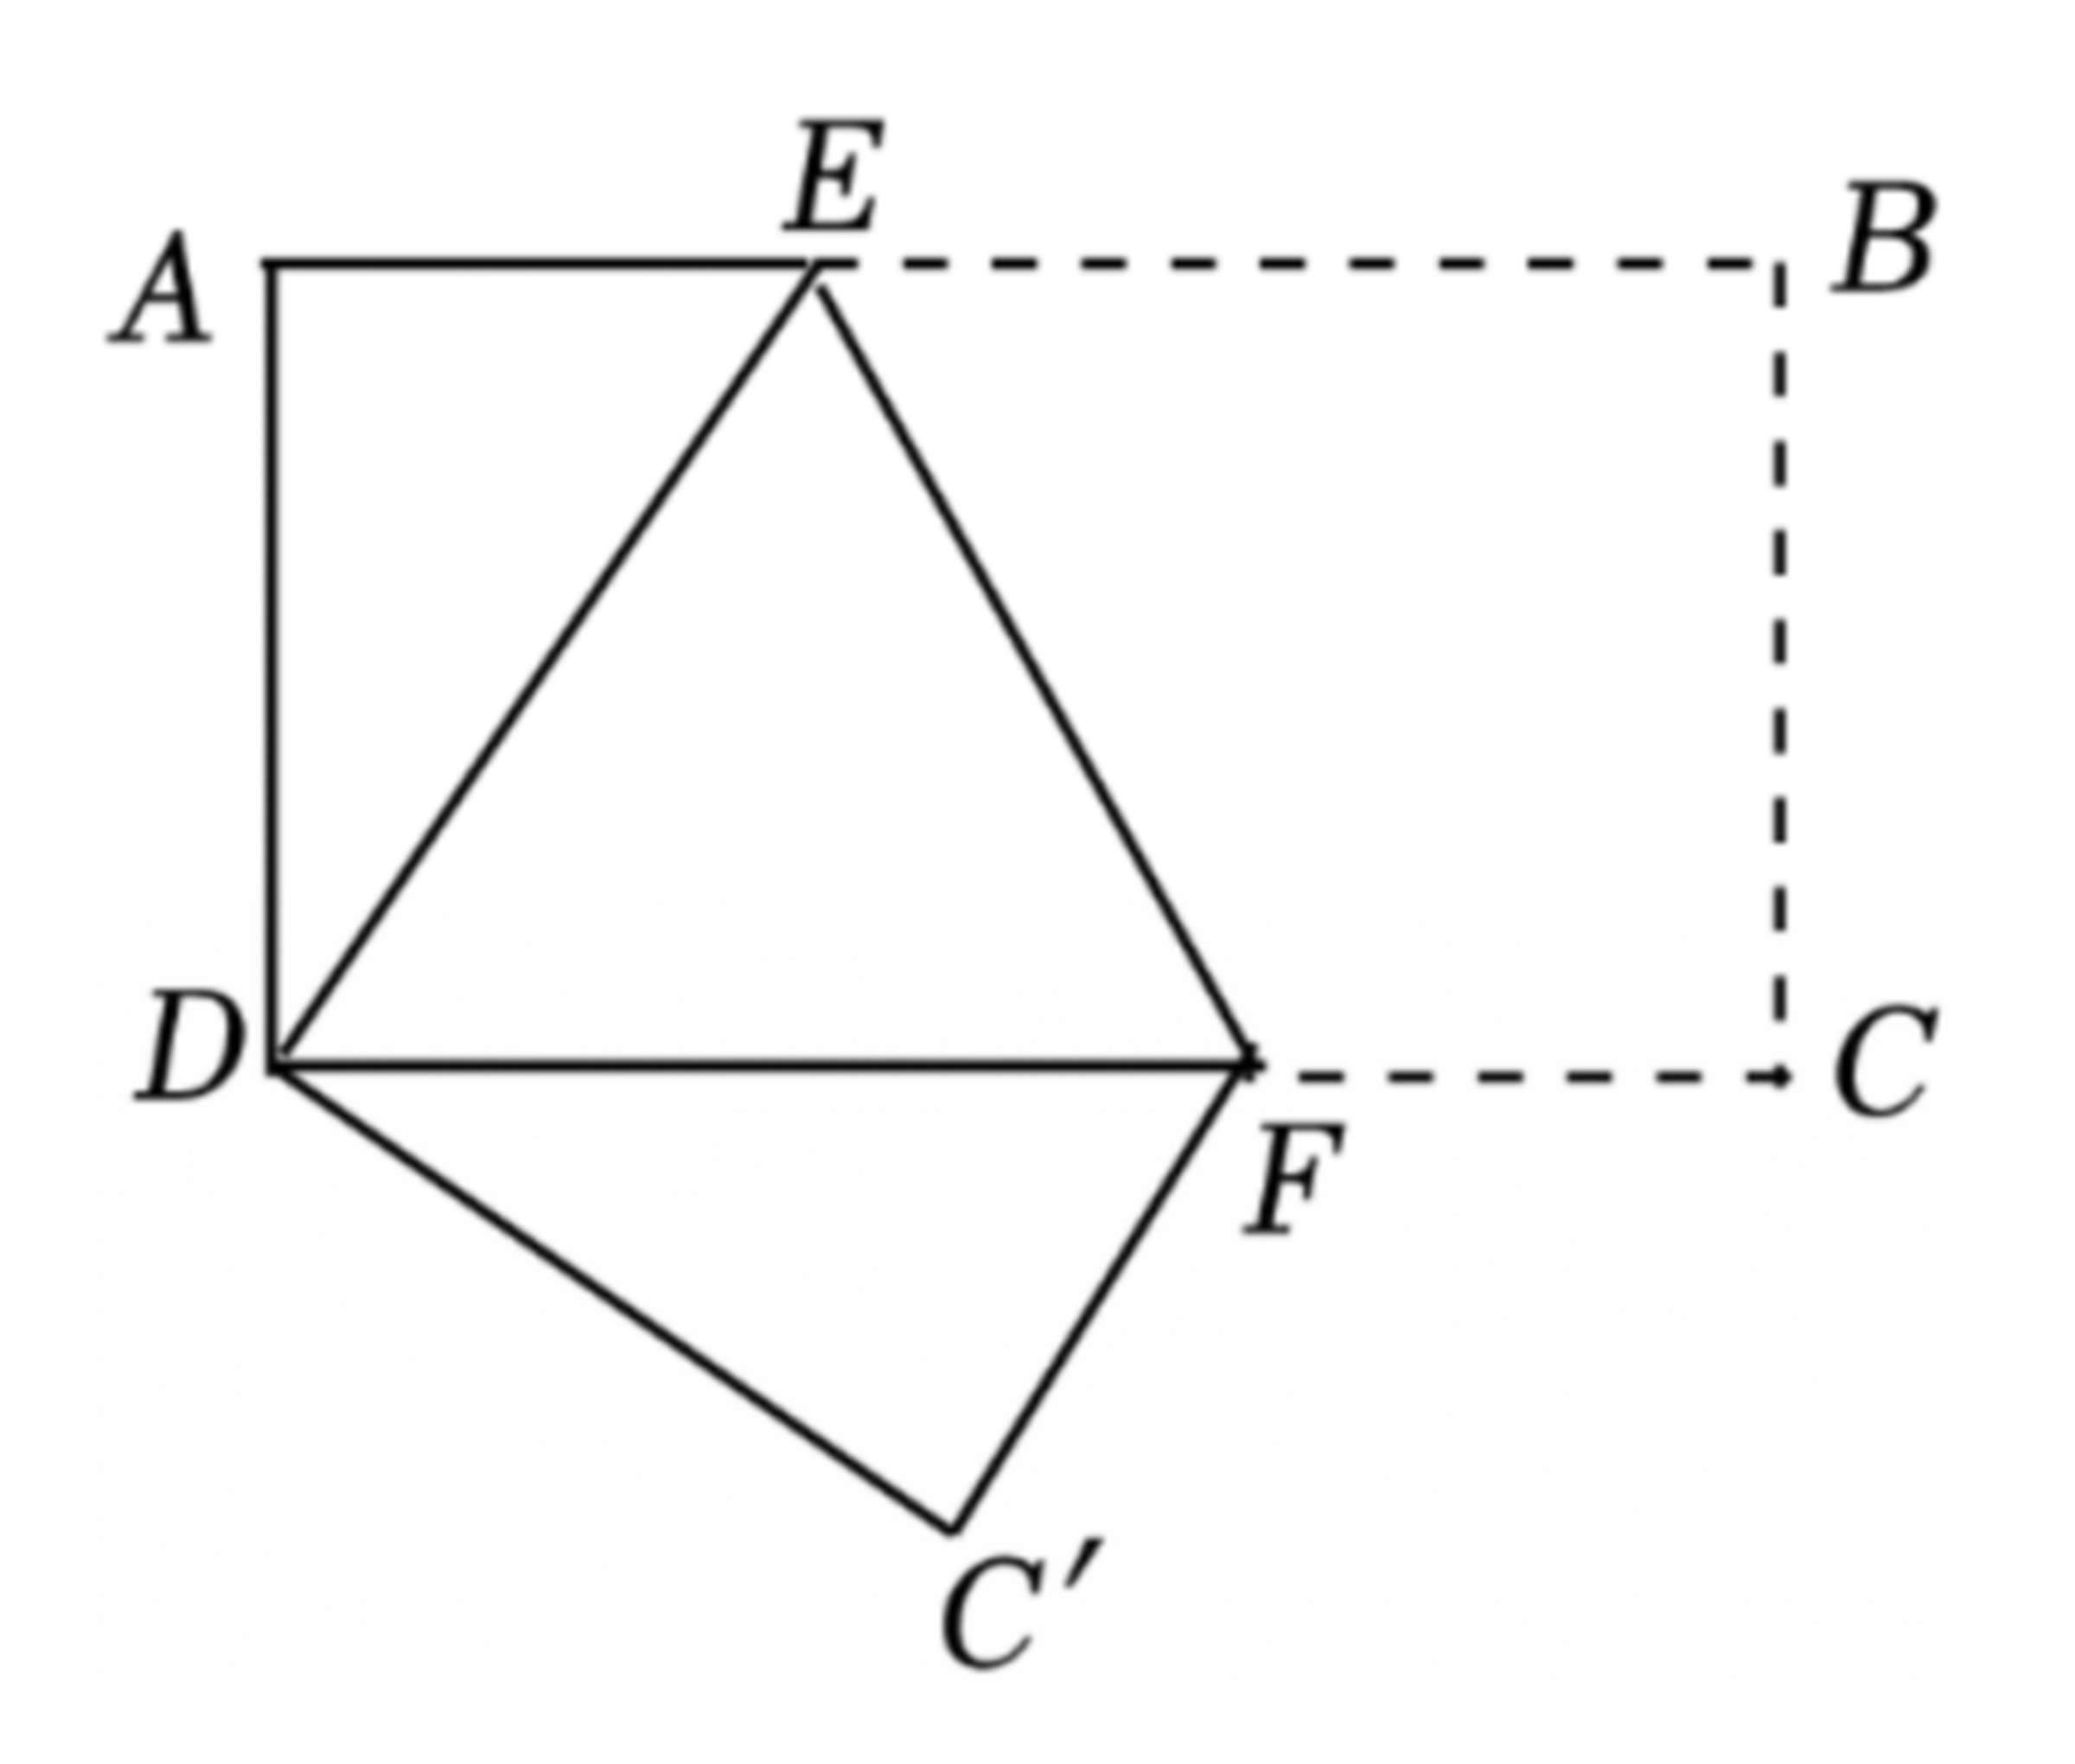
\includegraphics[width=0.40\textwidth]{figures/gao149_q11.png}
\end{center}

\ifanswer
\solbegin
\step{因为矩形 $ABCD(AB>AD)$ 的周长为 12，}
\step{在 $AB$ 和 $CD$ 边上分别取点 $E$ 和 $F$，将四边形 $BCFE$ 沿 $EF$ 折叠，}
\step{使点 $B$ 与点 $D$ 重合，此时点 $C$ 的对应点为 $C'$，}
\step{所以设 $AD=a$，$AB=b$，则 $2(a+b)=12$，}
\step{所以 $a+b=6$，且 $AB>AD$，所以 $b>a>0$，}
\step{设 $DF=x$，则 $C'F=b-x$，在 $Rt\triangle DC'F$ 中，$DC'=BC=a$，}% 几何三角形符号原卷印扁等边细线三角 $\triangle$，照录（放大 02 页确认）；$Rt$ 照录
\step{所以 $a^2+(b-x)^2=x^2$，解得 $x=\dfrac{a^2+b^2}{2b}$，}
\step{因此 $\triangle C'DF$ 的面积 $S=\dfrac{1}{2}\cdot DC'\cdot C'F=\dfrac{1}{2}\cdot a\cdot(b-x)$，}
\step{又 $b-x=b-\dfrac{(6-b)^2+b^2}{2b}=\dfrac{6(b-3)}{b}$，}
\step{所以 $S=\dfrac{1}{2}\cdot a\cdot\dfrac{6(b-3)}{b}=\dfrac{1}{2}\cdot(6-b)\cdot\dfrac{6(b-3)}{b}=\dfrac{3(6-b)(b-3)}{b}$}
\step{$=3\cdot\left(-b-\dfrac{18}{b}+9\right)$，又 $b+\dfrac{18}{b}\geqslant2\sqrt{b\cdot\dfrac{18}{b}}=6\sqrt{2}$，}
\step{当且仅当 $b=\dfrac{18}{b}$ 即 $b=3\sqrt{2}$ 时取等号，此时满足 $b>a$，}
\step{所以 $S\leqslant3\cdot(-6\sqrt{2}+9)=27-18\sqrt{2}$，故 $\triangle C'DF$ 面积的最大值为 $27-18\sqrt{2}$.}
\solend
\fi

% === Q12 === 解析内 3 幅三次函数曲线坐标图（仅答案版出）；解析 15 行（8 行 03 页＋7 行 04 页）
\item 已知 $m>0$，若存在 $t\in\R$，使得对任意 $x\in[0,m]$，不等式 $[(x-1)^2-t](x-t)\leqslant0$ 恒成立，则 $m$ 的最大值是\blankline[4.4em].

\ifanswer
\solbegin
\step{当 $t\leqslant0$ 时，$(x-1)^2-t\geqslant0$ 恒成立，}
\step{不等式 $[(x-1)^2-t](x-t)\leqslant0$ 的解集为 $x\leqslant t$，与 $x\in[0,m]$ 矛盾；}
\step{当 $t>0$ 时，不等式 $[(x-1)^2-t](x-t)\leqslant0\Leftrightarrow(x-1-\sqrt t)(x-1+\sqrt t)(x-t)\leqslant0$，}
\step{若 $t<1-\sqrt t$，即 $t\in\left(0,\dfrac{3-\sqrt5}{2}\right)$，}
\begin{center}
% 情形一 $t<1-\sqrt t$ 曲线图取 03 页右侧，去粉色水印、去色、4× LANCZOS 放大；仅答案版出
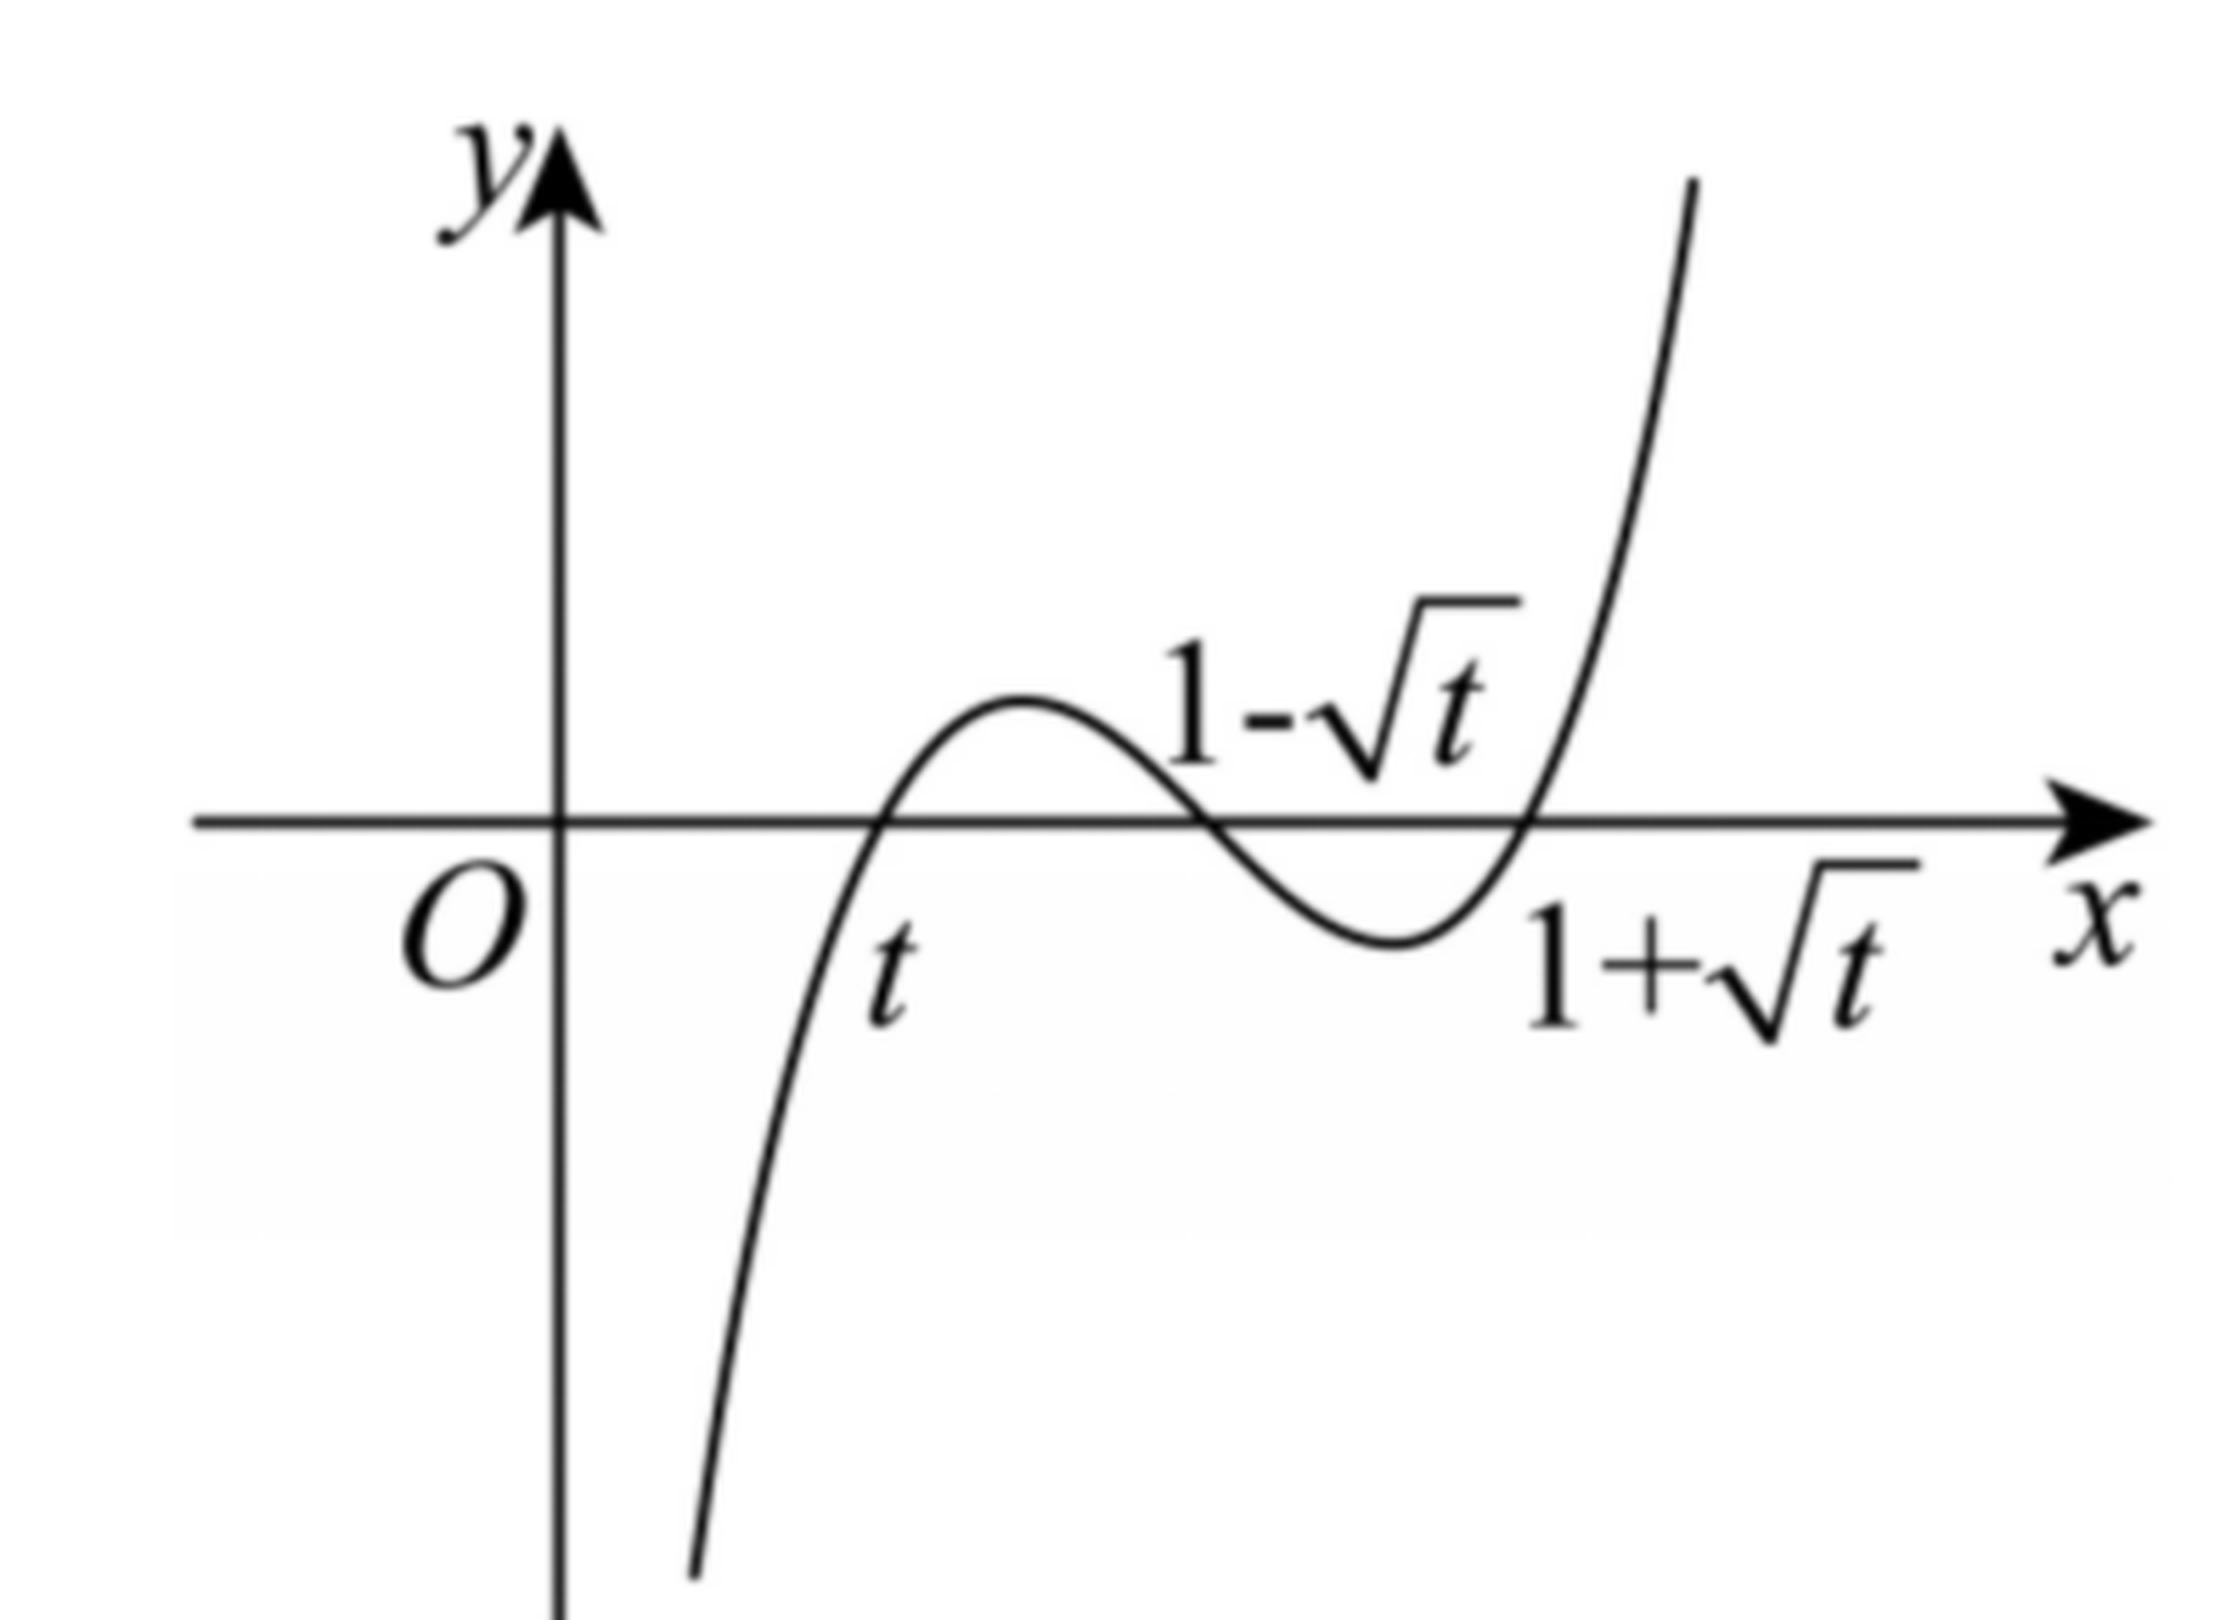
\includegraphics[width=0.40\textwidth]{figures/gao149_q12_a.png}
\end{center}
\step{则原不等式的解集为 $(-\infty,t]\cup[1-\sqrt t,1+\sqrt t]$，}
\step{当 $0<m\leqslant t$ 时，原不等式恒成立，因此}
\step{$m\in\left(0,\dfrac{3-\sqrt5}{2}\right)$；}
\step{若 $t=1-\sqrt t$，即 $t=\dfrac{3-\sqrt5}{2}$，则原不等式的解集为 $(-\infty,1+\sqrt t]$，}
\begin{center}
% 情形二 $t=1-\sqrt t$ 曲线图取 03 页右侧，去粉色水印、去色、4× LANCZOS 放大；仅答案版出
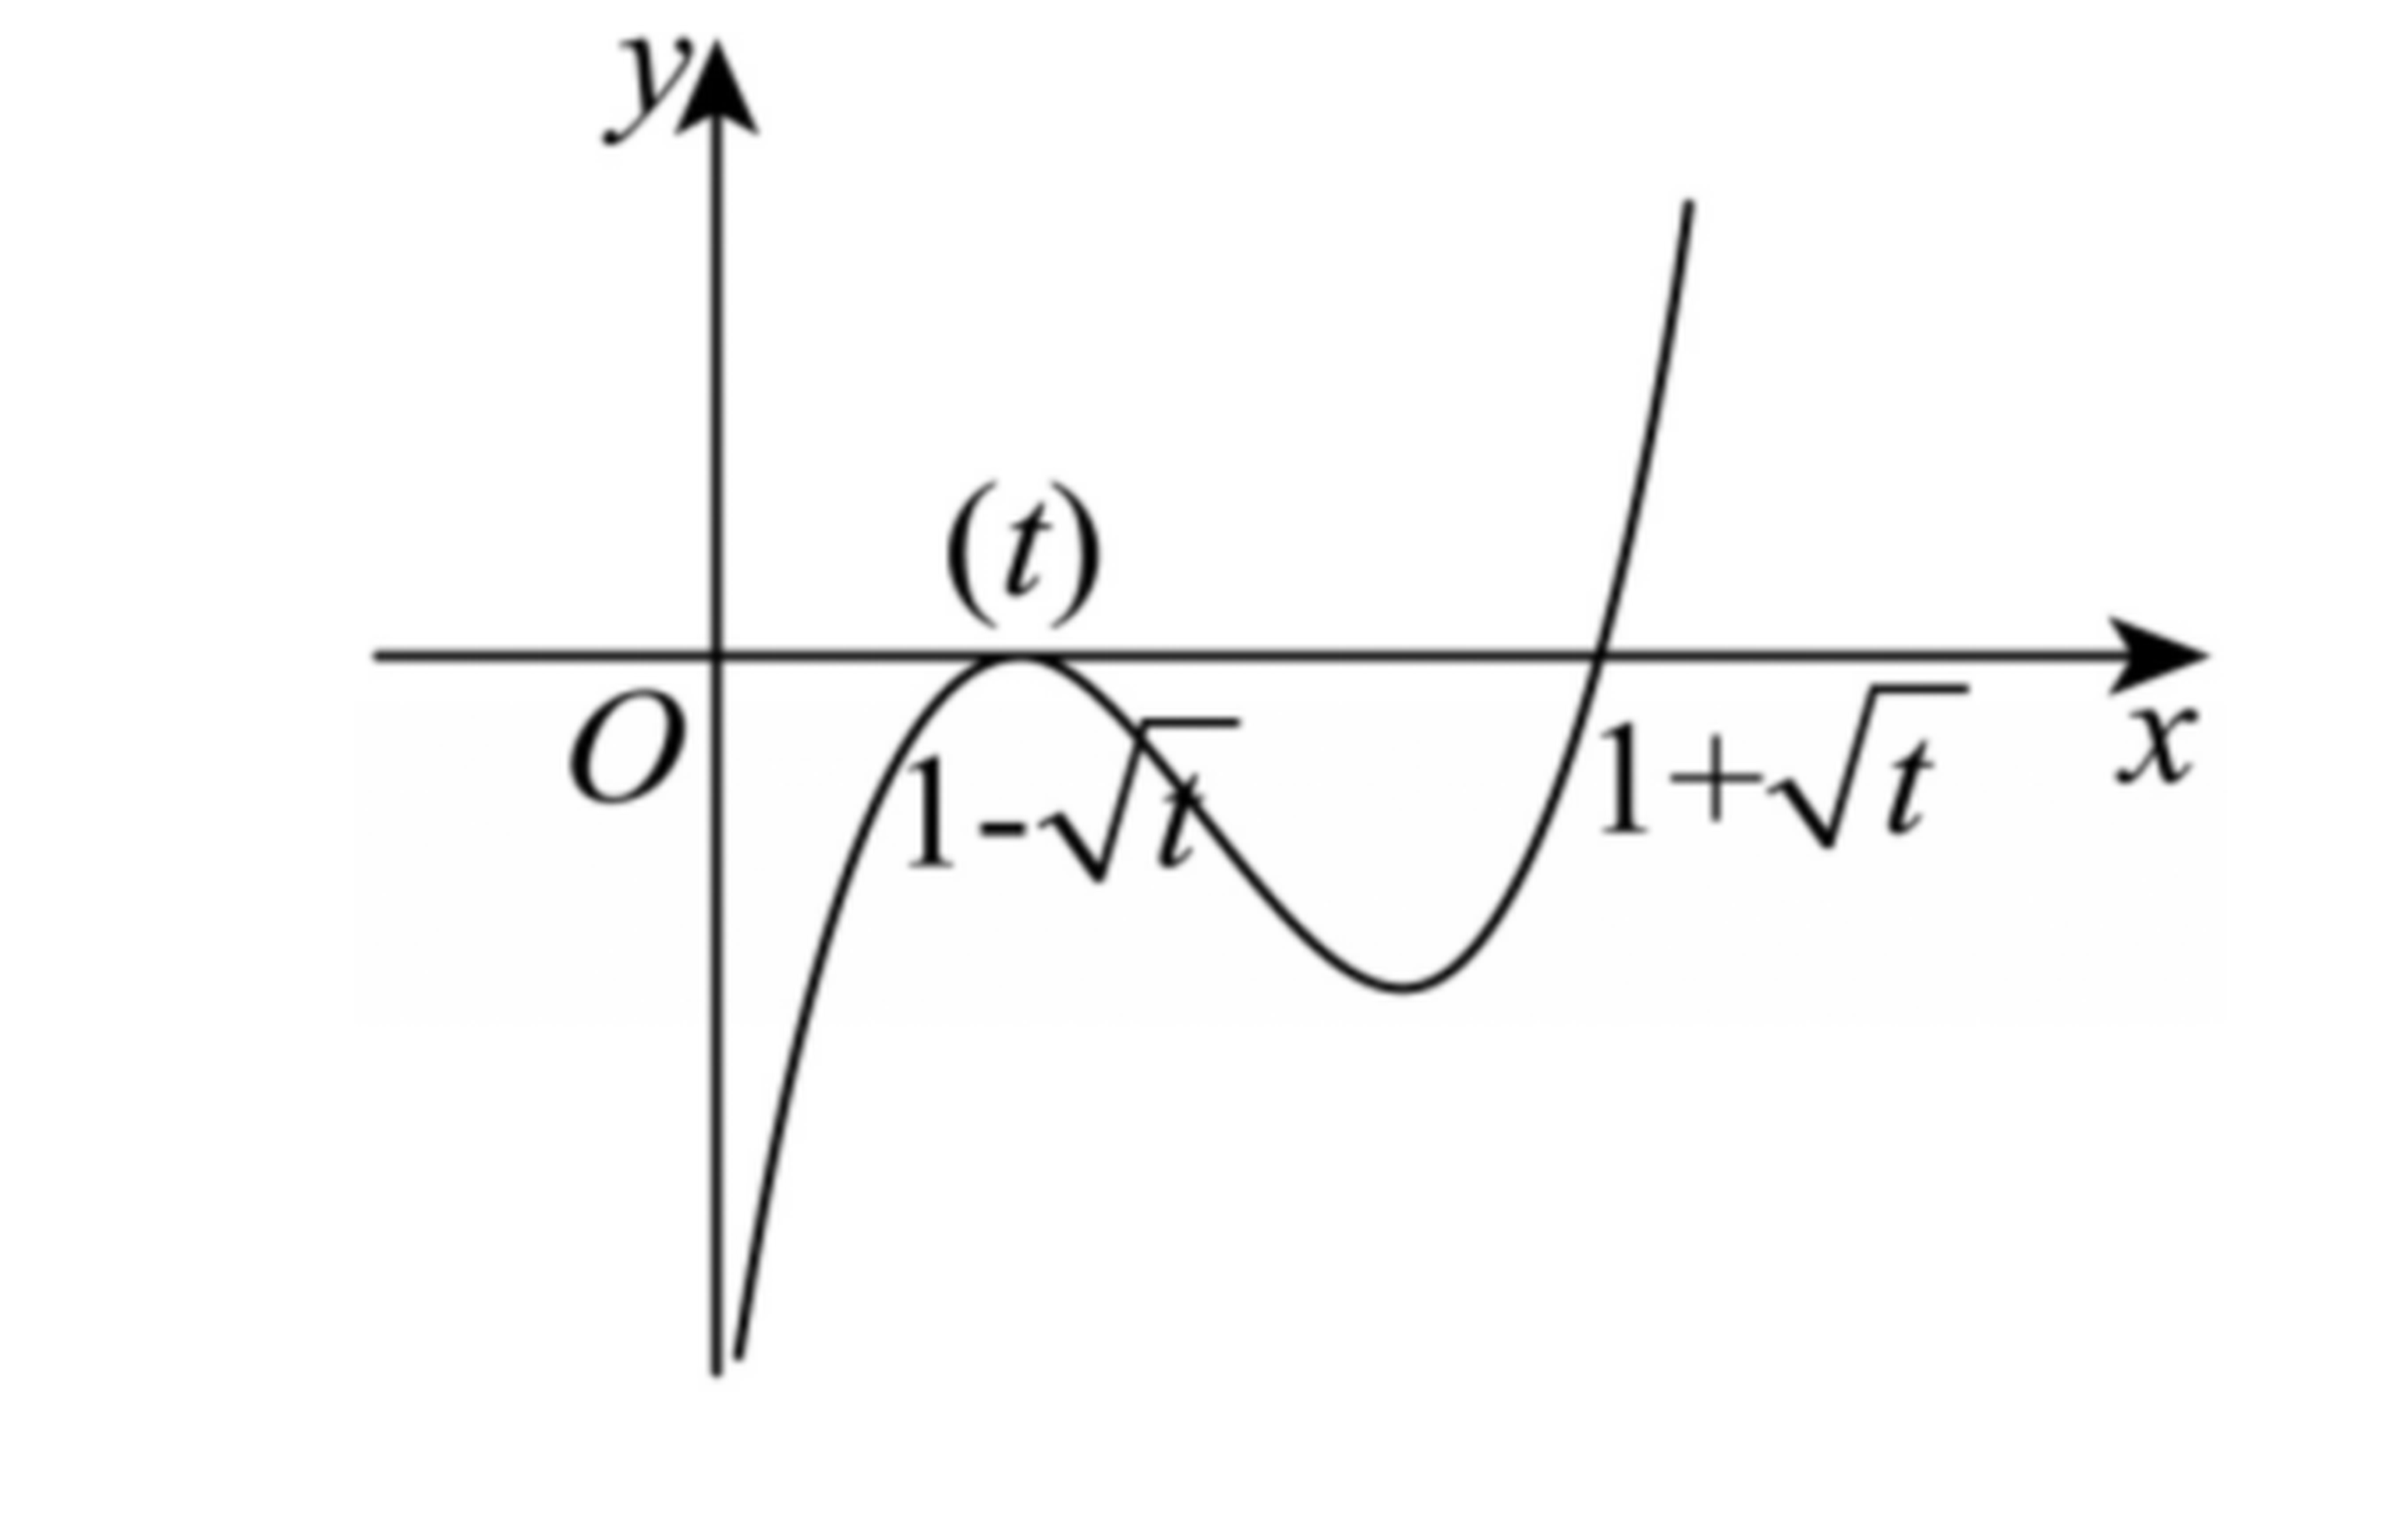
\includegraphics[width=0.40\textwidth]{figures/gao149_q12_b.png}
\end{center}
\step{当 $0<m\leqslant1+\sqrt t$ 时，原不等式恒成立，因此 $m\in\left(0,\dfrac{\sqrt5+1}{2}\right]$；}
\step{若 $1+\sqrt t>t>1-\sqrt t$，即 $t\in\left(\dfrac{3-\sqrt5}{2},\dfrac{3+\sqrt5}{2}\right)$，}
\begin{center}
% 情形三 $1+\sqrt t>t>1-\sqrt t$ 曲线图取 04 页右侧，去粉色水印、去色、4× LANCZOS 放大；仅答案版出
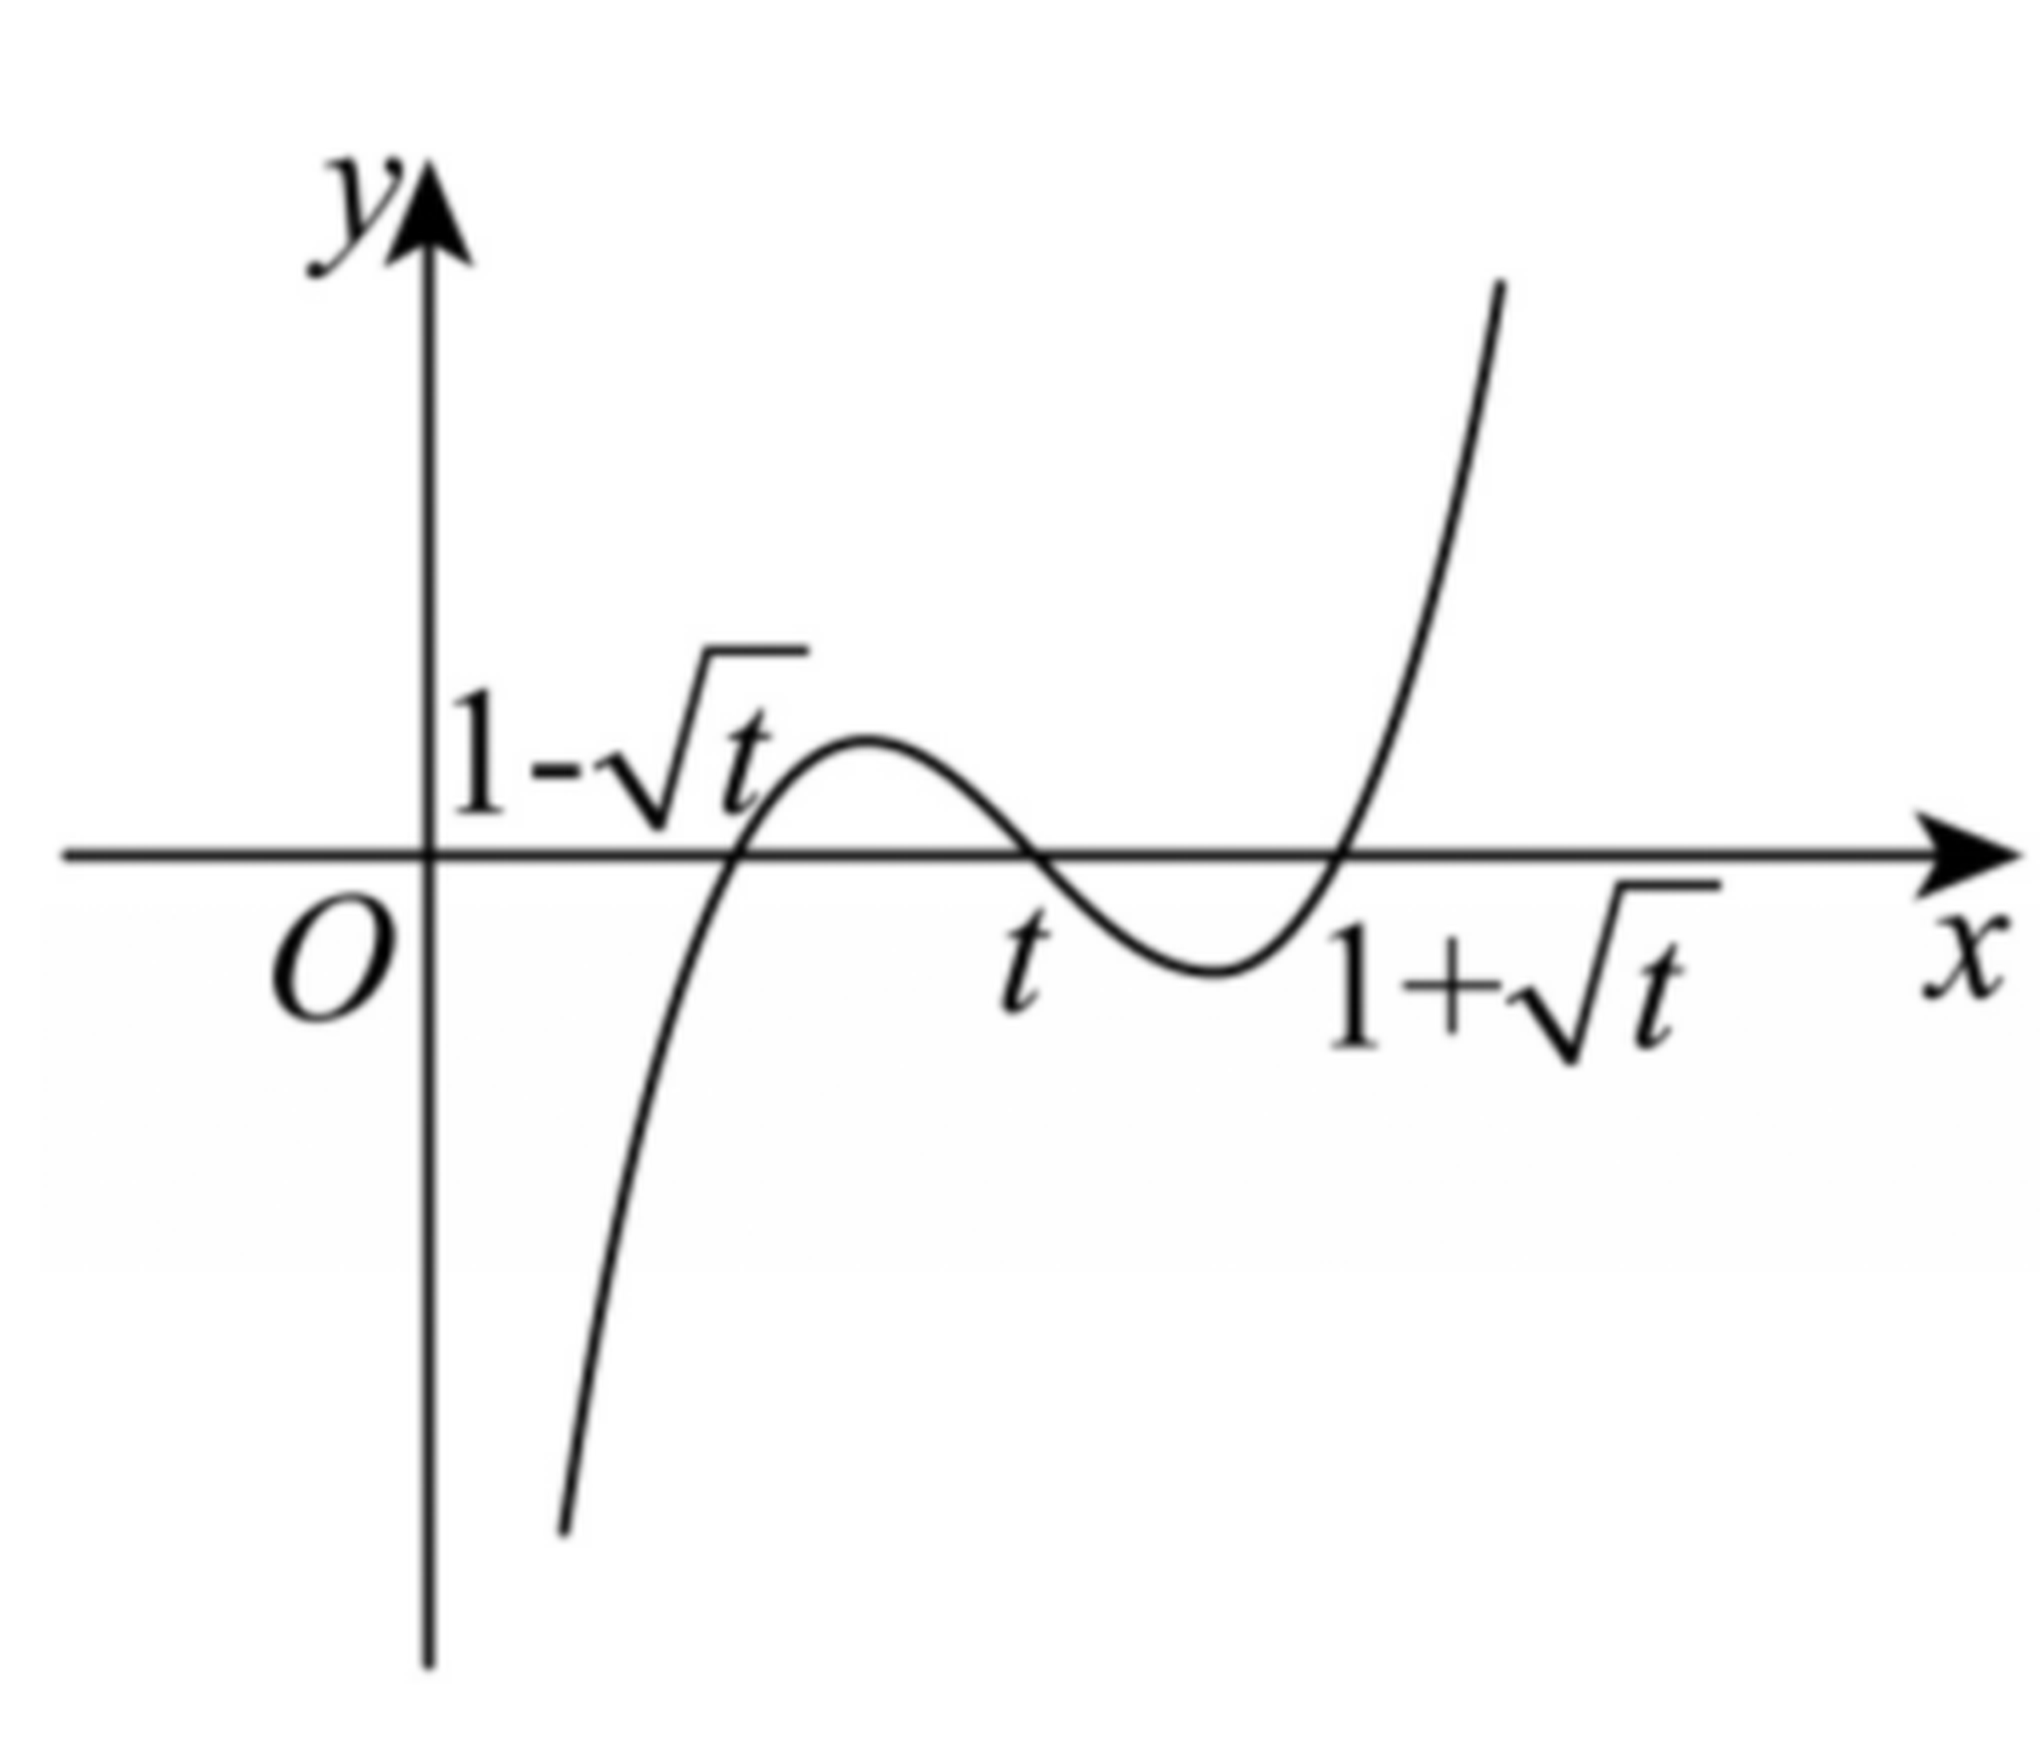
\includegraphics[width=0.40\textwidth]{figures/gao149_q12_c.png}
\end{center}
\step{则原不等式的解集为 $(-\infty,1-\sqrt t]\cup[t,1+\sqrt t]$，}
\step{当 $\begin{cases}1-\sqrt t>0\\1-\sqrt t\geqslant m\end{cases}$ 时，原不等式恒成立，此时 $t\in\left(\dfrac{3-\sqrt5}{2},1\right)$，$m\in\left(0,\dfrac{3-\sqrt5}{2}\right)$；}
\step{若 $t\geqslant1+\sqrt t$，即 $t\geqslant\dfrac{3+\sqrt5}{2}$，则取 $x=0$，$(t-1)t>0$，}
\step{原不等式不恒成立，不符合题意，}
\step{因此实数 $m$ 的取值范围是 $\left(0,\dfrac{\sqrt5+1}{2}\right]$，$m$ 的最大值是 $\dfrac{\sqrt5+1}{2}$.}
\solend
\fi

\end{enumerate}

\bigsec{二、选择题}

\begin{enumerate}
\setcounter{enumi}{12}

% === Q13 ===：答案"C"直接印在题干括号内、无【答案】/【解析】段，按 高一84 Q13／高一148 Q13 成例括号留空、另提 \ans{$C$}；四选项两行两列照原卷分行
\item 设 $ab>0$，则 $a>b$ 是 $\dfrac{1}{a}<\dfrac{1}{b}$ 的\mbox{（\quad）}

\keepwithprev
A. 充分不必要条件\qquad\qquad B. 必要不充分条件

C. 充要条件\qquad\qquad D. 既不充分又不必要条件

\ifanswer
\ans{$C$}
\fi

% === Q14 ===：$A\subset B$ 单线照录；四选项补集照原卷上划线 \overline{A}／\overline{B}；解析 1 行（由韦恩图得 B 对）
\item 已知集合 $A$、$B$ 非空，且 $A\subset B$，则下列式子中一定是空集的为\mbox{（\quad）}

\keepwithprev
A. $\overline{A}\cap B$\qquad B. $A\cap\overline{B}$\qquad C. $\overline{A}\cap\overline{B}$\qquad D. $\overline{A}\cup\overline{B}$

\ifanswer
\solbegin
\step{由韦恩图得 $B$ 对. 故选 $B$.}
\solend
\fi

% === Q15 ===："天文数字"弯引号照录；解析 2 行（首行在 04 页末、末行续 05 页顶）
\item 历史上数学计算方面的三大发明是阿拉伯数字、十进制和对数，其中对数的发明，大大缩短了计算时间，为人类研究科学和了解自然起了重大作用，对数运算对估算“天文数字”具有独特的优势. $2.5^{1000}$ 的估算值约为\mbox{（\quad）}

\keepwithprev
A. $10^{365}$\qquad B. $10^{379}$\qquad C. $10^{389}$\qquad D. $10^{398}$

\ifanswer
\solbegin
\step{$\lg 2.5^{1000}=1000\lg 2.5=1000(1-2\lg 2)\approx1000\times(1-0.602)=398$，}
\step{所以 $2.5^{1000}\approx10^{398}$. 故选 $D$.}
\solend
\fi

% === Q16 ===："完美集"新定义、圈数字①②文本模式；题干"若对任意 $x$，$y\in A$"用全角逗号、解析用顿号"$x$、$y\in A$"，两处照录不统一；解析 9 行
\item 设全集 $U=\R$，集合 $A$ 是一个非空数集，若对任意 $x$，$y\in A$，都有 $x+y\in A$、$xy\in A$，则称集合 $A$ 为一个“完美集”，给出以下命题：

①若 $A_1$、$A_2$ 都是“完美集”，且 $A_1\cap A_2\ne\varnothing$，则 $A_1\cap A_2$ 也是“完美集”；

②若 $A_1$、$A_2$ 都是“完美集”，则 $A_1\cup A_2$ 也是“完美集”.

下列说法正确的是\mbox{（\quad）}

\keepwithprev
A. ①②都是真命题\qquad\qquad B. ①是真命题，②是假命题

C. ①是假命题，②是真命题\qquad\qquad D. ①②都是假命题

\ifanswer
\solbegin
\step{由题意，全集 $U=\R$，集合 $A$ 是一个非空数集，}
\step{若对任意 $x$、$y\in A$，都有 $x+y\in A$、$xy\in A$，则称集合 $A$ 为一个“完美集”，}
\step{对于①，取 $x$、$y\in A_1\cap A_2$，则 $x\in A_1$，$x\in A_2$，$y\in A_1$，$y\in A_2$，}
\step{又 $A_1$、$A_2$ 是“完美集”，所以 $x+y\in A_1$，$xy\in A_1$，$x+y\in A_2$，$xy\in A_2$，}
\step{所以 $x+y\in A_1\cap A_2$，$xy\in A_1\cap A_2$，所以 $A_1\cap A_2$ 是“完美集”，故①正确；}
\step{对于②，取“完美集” $A_1=\{x\mid x=2k,k\in\Z\}$，$A_2=\{x\mid x=3k,k\in\Z\}$，}
\step{则 $2\in A_1$，$3\in A_2$，但 $2+3\notin A_1\cup A_2$，}
\step{即此时 $A_1\cup A_2$ 不是“完美集”，故②错误.}
\step{故选 $B$.}
\solend
\fi
\end{enumerate}

\bigsec{三、解答题}

\begin{enumerate}
\setcounter{enumi}{16}

% === Q17 ===："图像"（有亻）照录（Q17 题干与解析共 2 处）；绝对值 \lvert…\rvert；解析 7 行
\item 已知 $m\in\R$，$f(x)=(m^2-m-5)x^m$. 若 $y=f(x)$ 是幂函数，且其图像不经过原点.

(1) 求实数 $m$ 的值；

(2) 若 $f(a)=f(b)$ 且 $a\ne b$，求 $\lvert a+2\rvert+\lvert b-1\rvert$ 的最小值，并指出取到最小值时 $a$ 的取值范围.

\ifanswer
\solbegin
\step{(1) $f(x)=(m^2-m-5)x^m$ 是幂函数，得 $m^2-m-5=1$，即 $m^2-m-6=0$，}
\step{解得 $m=-2$ 或 $m=3$，又函数图像不经过原点，所以 $m=-2$($3$ 舍)；}
\step{(2) 由 (1) 得 $f(x)=x^{-2}=\dfrac{1}{x^2}$ 为偶函数，}
\step{$x<0$ 时，函数 $f(x)$ 严格增，$x>0$ 时，函数 $f(x)$ 严格减，}
\step{又 $f(a)=f(b)$ 且 $a\ne b$，所以 $a=-b$，且 $a\ne0$，$b\ne0$，}
\step{则 $\lvert a+2\rvert+\lvert b-1\rvert=\lvert a+2\rvert+\lvert-a-1\rvert=\lvert a+2\rvert+\lvert a+1\rvert$，}
\step{则 $\lvert a+2\rvert+\lvert b-1\rvert$ 的最小值为 $1$，取到最小值时 $a$ 的取值范围是 $[-2,-1]$.}
\solend
\fi

% === Q18 ===：判别式两形混用——(1) cases 块印高 \Delta、(2) 独立行印扁 \triangle，逐处照录不统一；解析 8 行
\item 已知命题 $p$：方程 $x^2+4x+m-1=0$ 有两个不等的负根；命题 $q$：方程 $4x^2+4x+m-2=0$ 无实根.

(1) 若 $p$ 为真命题，求 $m$ 的取值范围；

(2) 若 $p$、$q$ 两命题一真一假，求 $m$ 的取值范围.

\ifanswer
\solbegin
\step{(1) 若 $p$ 为真命题，即方程 $x^2+4x+m-1=0$ 有两个不等的负根；}
\step{必有 $\begin{cases}\Delta=16-4(m-1)>0\\m-1>0\end{cases}$，解得 $1<m<5$，即 $m$ 的取值范围为 $(1,5)$；}
\step{(2) 命题 $q$：方程 $4x^2+4x+m-2=0$ 无实根，}
\step{则有 $\triangle=16-16(m-2)<0$，解得 $m>3$，}
\step{若 $p$ 和 $q$ 有且只有一个为真命题，}
\step{若 $p$ 真 $q$ 假，必有 $\begin{cases}1<m<5\\m\leqslant3\end{cases}$，则有 $1<m\leqslant3$，}
\step{若 $p$ 假 $q$ 真，必有 $\begin{cases}m\leqslant1\text{ 或 }m\geqslant5\\m>3\end{cases}$，则有 $m\geqslant5$，}
\step{综上，$1<m\leqslant3$ 或 $m\geqslant5$.}
\solend
\fi

% === Q19 ===：$A\subseteq B$ 带下划线照录；解析 7 行（(2) 两组 cases 并排）
\item 已知 $m\in\R$，集合 $A=\left\{x\mid y=\sqrt{3-x}-\dfrac{1}{\sqrt{x-1}}\right\}$，集合 $B=\{x\mid 2m\leqslant x\leqslant1-m\}$.

(1) 若 $A\cup B=B$，求实数 $m$ 的取值范围；

(2) 若 $A\cap B=\varnothing$，求实数 $m$ 的取值范围.

\ifanswer
\solbegin
\step{(1) 函数 $y=\sqrt{3-x}-\dfrac{1}{\sqrt{x-1}}$，则 $\begin{cases}3-x\geqslant0\\x-1>0\end{cases}$，解得 $1<x\leqslant3$，}
\step{所以 $A=\{x\mid1<x\leqslant3\}$，}
\step{因为 $A\cup B=B$，所以 $A\subseteq B$，则 $\begin{cases}2m\leqslant1\\1-m\geqslant3\end{cases}$，解得 $m\leqslant-2$，}
\step{综上，实数 $m$ 的取值范围为 $(-\infty,-2]$；}
\step{(2) 当 $B=\varnothing$ 时，则 $2m>1-m$，解得 $m>\dfrac{1}{3}$，}
\step{当 $B\ne\varnothing$ 时，则 $\begin{cases}2m\leqslant1-m\\2m>3\end{cases}$ 或 $\begin{cases}2m\leqslant1-m\\1-m\leqslant1\end{cases}$，解得 $m\in\varnothing$ 或 $0\leqslant m\leqslant\dfrac{1}{3}$，}
\step{综上，实数 $m$ 的取值范围为 $[0,+\infty)$.}
\solend
\fi

% === Q20 ===：n 阶基本不等式推广；(3) 解析含 \overbrace{…}^{k} 上括号；(2) 解析"x=x=x=3(1-x)"三连等系原卷笔误、照录加注（见 ⑤）；解析 14 行
\item 教材中的基本不等式可以推广到 $n$ 阶：$n$ 个正数的算术平均数不小于它们的几何平均数，即对于任意的正数 $a_1$、$a_2$、$\cdots$、$a_n$，有 $\dfrac{a_1+a_2+\cdots+a_n}{n}\geqslant\sqrt[n]{a_1\cdot a_2\cdots a_n}$（$n\in\N$ 且 $n\geqslant2$），且等号当且仅当 $a_1=a_2=\cdots=a_n$ 时成立. 利用此结论解决下列问题：

(1) 若 $x$、$y$、$z>0$，求 $\dfrac{y}{x}+\dfrac{2z}{y}+\dfrac{4x}{z}$ 的最小值；

(2) 已知 $0<x<1$，求 $x^3(1-x)$ 的最大值，并求取得最大值时的 $x$ 的值；

(3) 对任意的正整数 $k$，判断 $\left(1+\dfrac{1}{k}\right)^k$ 与 $\left(1+\dfrac{1}{k+1}\right)^{k+1}$ 的大小关系，并证明.

\ifanswer
\solbegin
\step{(1) 因为 $x$、$y$、$z>0$，有 $\dfrac{y}{x}>0$，$\dfrac{2z}{y}>0$，$\dfrac{4x}{z}>0$}
\step{所以 $\dfrac{y}{x}+\dfrac{2z}{y}+\dfrac{4x}{z}\geqslant3\sqrt[3]{\dfrac{y}{x}\cdot\dfrac{2z}{y}\cdot\dfrac{4x}{z}}=3\sqrt[3]{8}=6$，}
\step{当且仅当 $\dfrac{y}{x}=\dfrac{2z}{y}=\dfrac{4x}{z}$ 时取等号，故 $\dfrac{y}{x}+\dfrac{2z}{y}+\dfrac{4x}{z}$ 的最小值为 $6$.}
\step{(2) 因为 $0<x<1$，所以 $1-x>0$，}
\step{$x^3(1-x)=\dfrac{1}{3}[x\cdot x\cdot x\cdot3(1-x)]\leqslant\dfrac{1}{3}\left[\dfrac{x+x+x+3(1-x)}{4}\right]^4=\dfrac{1}{3}\times\left(\dfrac{3}{4}\right)^4$}
\step{$=\dfrac{27}{256}$，当且仅当 $x=x=x=3(1-x)$，即 $x=3(1-x)$，$x=\dfrac{3}{4}$ 取等号，}% 原卷"x=x=x=3(1-x)"三连等，疑为四因子相等之误排，放大 08 页确认，照录未改（见 ⑤）
\step{所以 $0<x<1$ 时，$x^3(1-x)$ 的最大值是 $\dfrac{27}{256}$，取最大值时 $x=\dfrac{3}{4}$.}
\step{(3) 对任意 $k\in\N^*$，$\left(1+\dfrac{1}{k}\right)^k<\left(1+\dfrac{1}{k+1}\right)^{k+1}$.}
\step{证明：$\left(1+\dfrac{1}{k}\right)^k=\overbrace{\left(1+\dfrac{1}{k}\right)\cdot\left(1+\dfrac{1}{k}\right)\cdots\left(1+\dfrac{1}{k}\right)}^{k}\times1$}
\step{$\leqslant\left(\dfrac{\overbrace{\left(1+\dfrac{1}{k}\right)+\left(1+\dfrac{1}{k}\right)+\cdots+\left(1+\dfrac{1}{k}\right)}^{k}+1}{k+1}\right)^{k+1}$}
\step{$=\left(\dfrac{\overbrace{(1+1+\cdots+1)}^{k}+\overbrace{\left(\dfrac{1}{k}+\dfrac{1}{k}+\cdots+\dfrac{1}{k}\right)}^{k}+1}{k+1}\right)^{k+1}=\left(\dfrac{k+1+1}{k+1}\right)^{k+1}=\left(1+\dfrac{1}{k+1}\right)^{k+1}$，}
\step{当且仅当 $1+\dfrac{1}{k}=1$ 时取等号，}
\step{但是任意 $k\in\N^*$ 时 $1+\dfrac{1}{k}>1$，所以等号不成立，}
\step{故任意 $k\in\N^*$ 时，$\left(1+\dfrac{1}{k}\right)^k<\left(1+\dfrac{1}{k+1}\right)^{k+1}$.}
\solend
\fi

% === Q21 ===："减 k 集"新定义（引号内 k／数字两侧空格照录）；解析 26 行（续 10 页），含 ⑤ 三处原卷笔误照录
\item 定义：对于给定的整数 $k$，若非空集合 $A$ 满足如下 3 个条件：

① $A$ 是正整数集的子集；② $A\ne\{1\}$；

③对任意正整数 $x,y$，若 $x+y\in A$，则 $xy-k\in A$；则称集合 $A$ 为“减 $k$ 集”.

(1) 判断集合 $A=\{1,2\}$ 是否为“减 $0$ 集”？是否为“减 $1$ 集”？（无需说明理由）

(2) 证明：不存在“减 $2$ 集”；

(3) 是否存在“减 $1$ 集”？如果存在，求出所有“减 $1$ 集”；如果不存在，说明理由.

\ifanswer
\solbegin
\step{(1) 因为 $P\subseteq\N^*$，$P\ne\{1\}$，$1+1=2\in P$，$1\times1-0\in P$，}
\step{所以集合 $P=\{1,2\}$ 是“减 $0$ 集”；}
\step{因为 $P\subseteq\N^*$，$P\ne\{1\}$，$1+1=2\in P$，$1\times1-1\notin P$，}
\step{所以集合 $P=\{1,2\}$ 是“减 $1$ 集”；}% 按条件③应为"不是"，原卷径印"是"，放大 09 页确认，照录未改（见 ⑤）
\step{(2) 假设存在集合 $A$ 是“减 $2$ 集”，若 $x+y\in A$，则 $xy-2\in A$，}
\step{①当 $x+y=xy-2$ 时，有 $(x-1)(y-1)=3$，}
\step{则 $x$、$y$ 一个为 $2$，一个为 $4$，所以集合 $A$ 有元素 $6$，}
\step{但 $3+3\in A$，$3\times3-2\notin A$，与 $A$ 是“减 $2$ 集”矛盾；}
\step{②当 $x+y\ne xy-2$ 时，则 $x+y=xy-1$ 或 $x+y=xy-m$($m>2$)，}
\step{若 $x+y=xy-1$，$m=1$ 时，$M$ 为除 $1$ 以外的最小元素，}% 原卷"m=1"上文未显式定义，疑笔误，放大 09 页确认，照录未改（见 ⑤）
\step{则 $x=M-1$，$y=1$ 时，$xy-2=M-3$ 小于 $M$，}
\step{要符合题意，必须 $M=4$，}
\step{此时取 $x-2$，$y=2$，$xy-2=2$ 不属于 $A$，故不符合题意，}% 原卷"取 x−2"疑为"取 x=2"误排，放大 09 页确认，照录未改（见 ⑤）
\step{当 $m>2$ 时，$(x-1)(y-1)=m+1$，同样得出矛盾，}
\step{综上，不存在 $A$ 是“减 $2$ 集”.}
\step{(3) 存在“减 $1$ 集” $A$，则 $A\ne\{1\}$，}
\step{①假设 $1\in A$，则 $A$ 中除了元素 $1$ 以外，必然还含有其它元素，}
\step{假设 $2\in A$，$1+1\in A$，而 $1\times1-1\notin A$，所以 $2\notin A$，}
\step{假设 $3\in A$，$1+2\in A$，而 $1\times2-1\in A$，所以 $3\in A$，}
\step{所以 $A=\{1,3\}$，}
\step{假设 $4\in A$，$1+3\in A$，而 $1\times3-1\notin A$，所以 $4\notin A$，}
\step{假设 $5\in A$，$1+4\in A$，$1\times4-1\in A$，$2+3=5$，$2\times3-1\in A$，所以 $5\in A$，}
\step{所以 $A=\{1,3,5\}$，}
\step{以此类推，得 $A=\{1,3,5,\cdots,2n-1,\cdots\}$，($n\in\N^*$)，}
\step{所以所有的“减 $1$ 集”有 $\{1,3\}$，$\{1,3,5\}$，$\{1,3,5,7\}$，$\cdots$，$\{1,3,5,\cdots,2n-1,\cdots\}$，}
\step{$(n\in\N^*)$.}
\solend
\fi
\end{enumerate}

\end{document}
"
% 紧凑版：xelatex "\def\iscompact{1}% 高一149_青浦高级中学上外云间_期中.tex
%   —— 高一上数学"2026-2027 年青浦高级中学上外云间高一上期中"（试卷版/答案版/紧凑版）
% 试卷版：xelatex 高一149_青浦高级中学上外云间_期中.tex
% 答案版：xelatex "\def\isanswer{1}\input{高一149_青浦高级中学上外云间_期中.tex}"
% 紧凑版：xelatex "\def\iscompact{1}\input{高一149_青浦高级中学上外云间_期中.tex}"
%
% ① 原始材料：微信公众号"魔都数学加油站"文章，连载"27学年高一149"，原文标题
% "27学年高一149——2026-2027年上海市青浦高级中学上外云间高一上期中"；
% 原文链接：https://mp.weixin.qq.com/s/T7_nyoR1k0o_5og7FkDsyw 。
% 正文为 10 张 PNG 页（01/02/03/04/10 为 2560×3620，05/06/07/08/09 为 4762×6735，
% 同一篇各页分辨率混排，逐页按各自分辨率裁图核对，别按预览比例换算裁框）。
% 体例：混合体例讲评版——19 题中 Q6 只印【答案】、无【解析】；Q13 的答案"C"
%   直接印在题干括号内、无【答案】/【解析】段；其余 17 题印【解析】（逐题核实，见 ② ②）。
% 题目、答案、解析均据原图转录；卷面粉红色水印"魔都数学加油站"及公众号页脚未录入。
% 全卷插图清单（逐页通读 10 页确认）：1 幅题目配图 + 3 幅【解析】内配图：
%   · Q11 矩形 ABCD 折叠几何图（02 页右侧：A/B/C/D/E/F/C' 与虚线 EB、BC、FC），
%     题干"如图"处，题目配图、三版都出，裁 figures/gao149_q11.png；
%   · Q12【解析】内 3 幅三次函数曲线坐标图（03 页右侧两幅 + 04 页右侧一幅：
%     x/y 轴、O、t、1-\sqrt t、1+\sqrt t 等标注，分别对应 t<1-\sqrt t、
%     t=1-\sqrt t、1+\sqrt t>t>1-\sqrt t 三种情形），解析配图、仅答案版出，
%     分别裁 figures/gao149_q12_a.png／_b.png／_c.png，放 \ifanswer 内 \step 之间
%     （高一73 第 16 题成例）；
%   其余各页逐页确认无其它题目配图、无表格；Q14 解析"由韦恩图得 B 对"仅文字推导、
%   原卷并未印韦恩图；Q9／Q18／Q19 的 cases 块与 Q20(3) 的 \overbrace 为数学块（非图）；
%   10 页下半仅水印、无正文。4 图均取自原卷截图，去粉色水印、去色、4× LANCZOS 放大。
%
% 卷首标题：原卷印作"2026-2027 年青浦高级中学上外云间高一上期中"，年份区间按全稿
% 惯例排 en dash；原卷卷面未印副标题，本稿按同期中卷（高一140／141／143／144／145／
% 146／147／148）知识模块口径补出"集合与常用逻辑用语、不等式、函数"。
%
% 题号体例（逐页核实定稿）：本卷共 19 题——一、填空题 3—12（10 题）、
% 二、选择题 13—16（4 题）、三、解答题 17—21（5 题）。
% 三节分别 \setcounter{enumi}{2}／{12}／{16}。原卷从第 3 题起、无第 1、2 题，
% 本稿保留原题号；全卷无附加题节（Q21 解析末行"（n\in N^*）."为全卷收尾）。
%
% ② 与原卷的排版差异：
%   ① 原文从第 3 题起，本稿保留原题号；共 19 题三节；
%   ② 混合体例逐题核实：Q6（反证法"假设的内容"）只印【答案】、无【解析】，
%      按 高一140 第 5 题／高一145 Q3 成例提 \ans{}、不补造解析；Q13 答案"C"直接
%      印在题干括号内、全卷无该题【答案】/【解析】段，按 高一84 Q13／高一148 Q13
%      成例括号 \mbox{（\quad）} 留空、另提 \ans{$C$}；其余 17 题印【解析】、
%      用 \solbegin…\solend，选择题答案在解析末句"故选 X"（Q14 选 B、Q15 选 D、
%      Q16 选 B，逐个放大 04/05 页核实）、题干括号留空、不另提 \ans{}；
%      答案版【答案】/【解析】标记数 = 19（2 个 \ans ＋ 17 个 \solbegin）
%      = 全卷题数；
%   ③ 原卷卷面未印副标题，本稿按知识模块口径补出；
%   ④ 原卷填空横线按全稿惯例排 \blankline[4.4em]；选择题括号排 \mbox{（\quad）}、
%      选项段前按惯例加 \keepwithprev；Q13／Q16 四选项为两行两列、Q14／Q15
%      选项为一行，照原卷分行；解答题不留作答区、不加 \anspace（原卷为讲评版）；
%   ⑤ 数集：Q6"a,b\in N"、Q8"x\in R"、Q9"a\in R"／"解集为 R"、Q12"t\in R"、
%      Q16"U=R"、Q17"m\in R"、Q19"m\in R"、Q20"n\in N" 原卷印斜体 R/N，
%      按全稿惯例统一改 \R／\N；Q20(3)、Q21 的 $N^*$ 排 \N^*；Q16 解析
%      "$k\in Z$" 排 \Z。绝对值排 \lvert…\rvert（Q17），集合描述竖线排 \mid
%      （Q19、Q16 解析）；不等号按全稿惯例排 \leqslant／\geqslant；
%      补集照原卷上划线排 \overline{A}／\overline{B}（Q14 四选项）；空集
%      \varnothing（Q16、Q19、Q21）；
%   ⑥ 子集符号逐处照录不统一：Q4 题干"{1,2}⊆A⊂{1,2,3,4,5,6}" 前者印带下划线
%      ⊆、照录 \subseteq，后者印单线 ⊂、照录 \subset；Q10"A⊆{-1,1/2,2,3}"、
%      Q19 解析"A⊆B"、Q21 解析"P⊆N*" 均印带下划线 ⊆、照录 \subseteq；
%      Q14"A⊂B" 印单线 ⊂、照录 \subset（逐处放大 01/02/04/07/09 页确认，见 ④）；
%   ⑦ 子题标号 (1)(2)(3) 半角括号照录；圈数字 ①②③ 在文本模式（Q16 两命题、
%      Q21 三个条件与解析的①②）按 common.sty 划入 CJK 字符类渲染；cases 块整体
%      算一个印刷行；\left…\right 不得拆到不同 $…$ 组；数学式内 CJK 用 \text{}
%      （Q18 解析 cases 块"\text{或}"）；Q11 解析"Rt\triangle DC'F" 的 Rt 照录；
%   ⑧ 题干／解析中的中文弯引号按原卷照录：Q6" 已知 a,b\in N，若 ab 能被 5 整除，
%      那么 a、b 中至少有一个能被 5 整除 "（开引号后紧跟"已知"、闭引号后空格接"时"）、
%      Q15"天文数字"、Q16"完美集"、Q21"减 k 集""减 0 集""减 1 集""减 2 集"
%      （引号内 k／数字两侧有空格），注释内一律 ASCII 引号；
%   ⑨ 半角逗号在数学组之间是全稿惯例、非笔误（Q8"$a>0,a\ne1,x\in\R$"、
%      Q21 题干"$x,y$" 等），逐处照录别改；Q16 题干"若对任意 $x$，$y\in A$"
%      用全角逗号而解析用顿号"$x$、$y\in A$"，两处不同均照录；行末西文句点
%      照录为 ASCII `.`；行中全角逗号／顿号照录；
%   ⑩ "图像／图象"逐处放大核：Q10 题干与解析共 6 处均印"图象"（象，无亻）；
%      Q17 题干"其图像不经过原点"与解析"又函数图像不经过原点" 2 处印"图像"
%      （像，有亻），逐处照录未统一改动（放大 02/05/06 页确认）；
%   ⑪ 判别式 Δ/△ 混用是照录项：Q9 解析 cases 块"Δ=4(a−2)²+16(a−2)<0"、
%      Q18(1) cases 块"Δ=16−4(m−1)>0" 两处印等腰偏高粗三角 \Delta；
%      Q18(2) 独立行"△=16−16(m−2)<0" 印扁等边细线三角 \triangle，
%      逐处放大判断、照录不统一（参照 高一142／144／145／146／148 头注④口径）；
%      另 Q11 题干"△C'DF 面积"与解析 3 处"△"（含"Rt△DC'F"）共 4 处几何
%      三角形符号亦印扁细线三角，照录 \triangle（非判别式，字形同类，见 ④）；
%   ⑫ 一条 \step = 原卷解析的一个印刷行，cases 块整体算一个印刷行；别把原卷折行
%      并起来、别把一行拆多条。Q11 十三行（7 行在 02 页＋6 行在 03 页）、
%      Q12 十五行（8 行在 03 页＋7 行在 04 页）、Q16 九行、Q21 二十六行
%      （续 10 页）均按印刷行逐条断，不丢行；
%   ⑬ 配图：Q11 题目配图（三版都出）放 \item 内题干之后 \begin{center}，
%      大图块加 \needvspace{8cm} 守卫把整块推走（守卫放 \item 之前，见
%      高一145 Q14/Q20 成例与切页审计 B 类坑）；Q12 三幅解析配图（仅答案版出）
%      放 \ifanswer 内 \solbegin…\solend 的 \step 之间；三版切页审计均"合计异常：无"；
%   ⑭ 跨页续印按题合并：Q3/4/5 在 01 页；Q6/7/8 题干与解析在 01 页；
%      Q9 题干在 01 页末、解析 4 行在 02 页顶；Q10 题干＋解析在 02 页；
%      Q11 题干＋图＋解析前 7 行在 02 页、解析后 6 行续 03 页顶；
%      Q12 题干＋解析首行在 03 页末、解析续 7 行在 03 页下半＋7 行在 04 页顶，
%      "二、选择题"标题在 04 页下半；Q13/14 题干＋选项＋Q14 解析在 04 页下半；
%      Q15 题干＋选项＋解析首行在 04 页末、末行"所以 2.5^1000≈10^398. 故选 D."
%      续 05 页顶；Q16 题干＋选项＋解析 9 行在 05 页、"三、解答题"标题＋
%      Q17 题干首句在 05 页末；Q17(2)＋解析 7 行、Q18 题干＋解析前 6 行在 06 页；
%      Q18 解析末 2 行续 07 页顶；Q19 题干＋解析 4 行在 07 页上半、
%      解析续 3 行在 07 页下半；Q20 题干(1) 在 07 页末、题干(2)(3)＋解析(1)(2)
%      在 08 页上半、(3) 解析含 \overbrace 的证明在 08 页下半、末行
%      "故任意 k∈N* 时…"续 09 页顶；Q21 题干＋解析(1)(2)(3) 前段在 09 页、
%      解析(3) 后半 9 行续 10 页上半（10 页下半仅水印、无正文）。
%      本稿按题连排，不丢行、不并折行；
%   ⑮ 原卷解析内无红色"法一／法二"之类小标题，故本卷无 \stepm；水印
%      "魔都数学加油站"红色不录入。
%
% ③ 行数复核：一条 \step／\stepm = 原卷解析的一个印刷行，cases 块作一个印刷行计。
%   逐题数（主会话逐页核对定稿）：Q3：1；Q4：2；Q5：2；Q6：0（只印【答案】、
%   提 \ans{}）；Q7：1；Q8：1；Q9：4；Q10：5；Q11：13；Q12：15；
%   Q13：0（答案印在题干括号内、另提 \ans{}）；Q14：1；Q15：2；Q16：9；
%   Q17：7；Q18：8；Q19：7；Q20：14；Q21：26。
%   合计 118 条 \step（本卷无 \stepm：解析内无红色"法一／法二"类小标题），
%   与原卷逐题印刷行相等。全卷 17 题设 \solbegin…\solend ＋ 2 处 \ans{}，
%   答案版【答案】/【解析】标记数 = 19 = 全卷题数。
%
% ④ 判别式／子集符号结论（逐处放大原图照录、不得统一，主会话像素级复核）：
%   判别式全卷 3 处，两形混用逐处照录不统一（参照 高一142／144／145／146／148 头注④）：
%     · Q9 解析 cases 块"Δ=4(a−2)²+16(a−2)<0" 原卷印等腰偏高粗三角（高>宽、
%       粗笔画），照录 \Delta（放大 02 页 /tmp/gao149/z/t02_q9_delta2.png 确认）；
%     · Q18(1) cases 块"Δ=16−4(m−1)>0" 原卷印等腰偏高粗三角（高>宽、粗笔画），
%       照录 \Delta（放大 06 页 /tmp/gao149/z/t06_q18a.png 确认）；
%     · Q18(2) 独立行"△=16−16(m−2)<0" 原卷印扁等边细线三角（宽>高、细线），
%       照录 \triangle（放大 06 页 /tmp/gao149/z/t06_q18b.png 与 Q18(1) 并排确认）。
%   另 Q11 题干"△C'DF"与解析 3 处"△"（含"Rt△DC'F"）共 4 处几何三角形符号
%     亦印扁等边细线三角，照录 \triangle（放大 02 页
%     /tmp/gao149/z/t02_q11_tri2.png 确认），与 Q9／Q18(1) 判别式 \Delta 两形不统一。
%   子集／补集：Q4 题干"{1,2}⊆A⊂{1,2,3,4,5,6}" 前者带下划线 ⊆、照录 \subseteq，
%     后者单线 ⊂、照录 \subset（放大 01 页 /tmp/gao149/z/t01_q3q4.png 确认）；
%     Q10"A⊆{-1,1/2,2,3}"、Q19 解析"A⊆B"、Q21 解析"P⊆N*" 三处带下划线 ⊆、
%     照录 \subseteq；Q14"A⊂B" 单线 ⊂、照录 \subset（放大 04 页
%     /tmp/gao149/z/t04_q14_sub2.png 确认）；Q14 四选项补集 \overline{A}／\overline{B}
%     照原卷上划线；空集 \varnothing（Q16、Q19、Q21）；Q19／Q16 解析集合描述竖线
%     \mid；数集 \R／\N／\N^*／\Z 归一见 ② ⑤。
%
% ⑤ 存疑照录（放大原图确认，照录未改、正文对应处另有 % 注）：
%   1. Q21 解析(1) 第二组"因为 P⊆N*，P≠{1}，1+1=2∈P，1×1−1∉P，所以集合
%      P={1,2} 是"减 1 集"" —— 按条件③（x=y=1 时 xy−1=0 须∈P）应为"不是"，
%      原卷却径印"是"，放大 09 页 /tmp/gao149/z/t09_q21_sol1.png 确认，照录未改
%      （疑为原卷结论笔误）。
%   2. Q21 解析(2)"此时取 x−2，y=2，xy−2=2 不属于 A" —— 按上下文应为
%      "取 x=2"（x−2 疑为 x=2 的误排），放大 09 页
%      /tmp/gao149/z/t09_q21_sol2.png 确认，照录未改。
%   3. Q21 解析(2)"若 x+y=xy−1，m=1 时，M 为除 1 以外的最小元素" 中 $m=1$
%      上文未显式定义 m（仅"x+y=xy−m(m>2)"中出现），放大 09 页确认，照录未改。
%   4. Q20 解析(2)"当且仅当 x=x=x=3(1−x)" 三个 x 连等，疑为原卷排印（应为
%      四个因子 x,x,x,3(1−x) 相等），放大 08 页
%      /tmp/gao149/z/t08_q20_sol2.png 确认，照录未改。
%   5. Q6 只印【答案】、Q13 答案印题干括号内，两题均无【解析】，按成例提
%      \ans{}、未补造解析（见 ② ②）。
%   6. 判别式 Q9／Q18(1) 高 \Delta 与 Q18(2)／Q11 扁 \triangle 两形混用，逐处
%      照录不统一（见 ④）；"图像／图象" Q10 用"图象"、Q17 用"图像"，
%      逐处照录未统一（见 ② ⑩）。
%   全卷除此 6 类外未发现其它笔误／自相矛盾处。
%
% ⑥ 跨页续印按题合并说明：见 ② ⑭。
%
\documentclass[a4paper,11pt]{article}
\usepackage{common}

\begin{document}

\examtitlest[3]{2026--2027 年青浦高级中学上外云间高一上期中}{集合与常用逻辑用语、不等式、函数}

\bigsec{一、填空题}

\begin{enumerate}
\setcounter{enumi}{2}

% === Q3 === 根式化分数指数幂；解析 1 行
\item 根式 $\sqrt{a\sqrt a}$ 化成分数指数幂是\blankline[4.4em].

\ifanswer
\solbegin
\step{$\sqrt{a\sqrt a}=\sqrt{a\cdot a^{\frac{1}{2}}}=\sqrt{a^{1+\frac{1}{2}}}=\sqrt{a^{\frac{3}{2}}}=a^{\frac{3}{2}\times\frac{1}{2}}=a^{\frac{3}{4}}$.}
\solend
\fi

% === Q4 === 题干两种子集符号逐处照录（\subseteq 带下划线／\subset 单线）；解析 2 行
\item 满足 $\{1,2\}\subseteq A\subset\{1,2,3,4,5,6\}$ 的集合 $A$ 共有\blankline[4.4em]个.

\ifanswer
\solbegin
\step{集合 $A$ 满足 $\{1,2\}\subseteq A\subset\{1,2,3,4,5,6\}$，}% 前者带下划线 $\subseteq$、后者单线 $\subset$，逐处照录不统一（放大 01 页确认）
\step{所以集合 $A$ 的个数为集合 $\{3,4,5,6\}$ 的真子集的个数，即为 $2^4-1=15$ 个.}
\solend
\fi

% === Q5 === 解析 2 行
\item 不等式 $\dfrac{2x+1}{x-1}\leqslant0$ 的解集为\blankline[4.4em].

\ifanswer
\solbegin
\step{不等式 $\dfrac{2x+1}{x-1}\leqslant0$ 可化为 $(2x+1)(x-1)\leqslant0$，且 $x-1\ne0$，解得 $-\dfrac{1}{2}\leqslant x<1$，}
\step{即原不等式的解集为 $\left[-\dfrac{1}{2},1\right)$.}
\solend
\fi

% === Q6 === 原卷只印【答案】、无【解析】，按 高一140 第 5 题／高一145 Q3 成例提 \ans{}、不补造解析；弯引号与空格照录
\item 用反证法证明命题 “已知 $a,b\in\N$，若 $ab$ 能被 5 整除，那么 $a$、$b$ 中至少有一个能被 5 整除” 时，假设的内容应该是\blankline[4.4em].

\ifanswer
\ans{$a$、$b$ 都不能被 5 整除}
\fi

% === Q7 === 解析 1 行
\item 若 $\log_3(\log_4 x)=1$，则 $x=$\blankline[4.4em].

\ifanswer
\solbegin
\step{$\log_3(\log_4 x)=1$，则 $\log_4 x=3$，故 $x=64$.}
\solend
\fi

% === Q8 === 半角逗号在数学组之间照录；解析 1 行
\item 已知 $a>0,a\ne1,x\in\R$，且 $a^{2x}=2$，则 $\dfrac{a^{3x}+a^{-3x}}{a^x+a^{-x}}$ 的值为\blankline[4.4em].

\ifanswer
\solbegin
\step{$\dfrac{a^{3x}+a^{-3x}}{a^x+a^{-x}}=a^{2x}-1+a^{-2x}=2-1+\dfrac{1}{2}=\dfrac{3}{2}$.}
\solend
\fi

% === Q9 === 题干在 01 页末、解析 4 行在 02 页顶；cases 块整体算 1 行；判别式高 \Delta
\item 已知 $a\in\R$，若关于 $x$ 的不等式 $(a-2)x^2+2(a-2)x-4<0$ 的解集为 $\R$，则实数 $a$ 的取值范围是\blankline[4.4em].

\ifanswer
\solbegin
\step{当 $a=2$ 时，不等式化为 $-4<0$ 对于任意实数 $x$ 都成立，因此 $a=2$ 满足题意；}
\step{当 $a\ne2$ 时，要使关于 $x$ 的不等式 $(a-2)x^2+2(a-2)x-4<0$ 的解集为 $\R$，}
\step{则 $\begin{cases}a-2<0\\\Delta=4(a-2)^2+16(a-2)<0\end{cases}$，解得 $-2<a<2$.}% cases 块整体算一个印刷行；判别式原卷印等腰偏高粗三角 $\Delta$，照录（放大 02 页确认）
\step{综上，$a$ 的取值范围为 $(-2,2]$.}
\solend
\fi

% === Q10 === "图象"（象，无亻）逐处照录；\subseteq 带下划线；解析 5 行
\item 已知集合 $A=\{\alpha,\beta\}$，且 $A\subseteq\left\{-1,\dfrac{1}{2},2,3\right\}$，函数 $f(x)=x^\alpha$ 与 $g(x)=x^\beta$ 的图象有两个交点，则满足条件的不同集合 $A$ 有\blankline[4.4em]个.

\ifanswer
\solbegin
\step{函数 $y=x^{-1}$ 与 $y=x^{\frac{1}{2}}$，$y=x^2$，$y=x^3$ 的图象分别有 1 个，1 个，2 个交点；}
\step{函数 $y=x^{\frac{1}{2}}$ 与 $y=x^2$，$y=x^3$ 的图象都有 2 个交点；}
\step{函数 $y=x^2$ 与 $y=x^3$ 的图象有 2 个交点，}
\step{函数 $f(x)=x^\alpha$ 与 $g(x)=x^\beta$ 的图象若只有 2 个交点，}
\step{则 $A=\{-1,3\}$ 或 $\left\{\dfrac{1}{2},2\right\}$ 或 $\left\{\dfrac{1}{2},3\right\}$ 或 $\{2,3\}$，有 4 个.}
\solend
\fi

% === Q11 === 题目配图（矩形折叠，三版都出）；\needvspace{8cm} 守卫放 \item 之前；解析 13 行（7 行 02 页＋6 行 03 页）
\needvspace{8cm}
\item 如图，矩形 $ABCD(AB>AD)$ 的周长为 12，在 $AB$ 和 $CD$ 边上分别取点 $E$ 和 $F$，将四边形 $BCFE$ 沿 $EF$ 折叠，使点 $B$ 与点 $D$ 重合，此时点 $C$ 的对应点为 $C'$，则 $\triangle C'DF$ 面积的最大值为\blankline[4.4em].

\begin{center}
% 矩形 ABCD 折叠几何图取 02 页右侧，去粉色水印、去色、4× LANCZOS 放大；三版都出
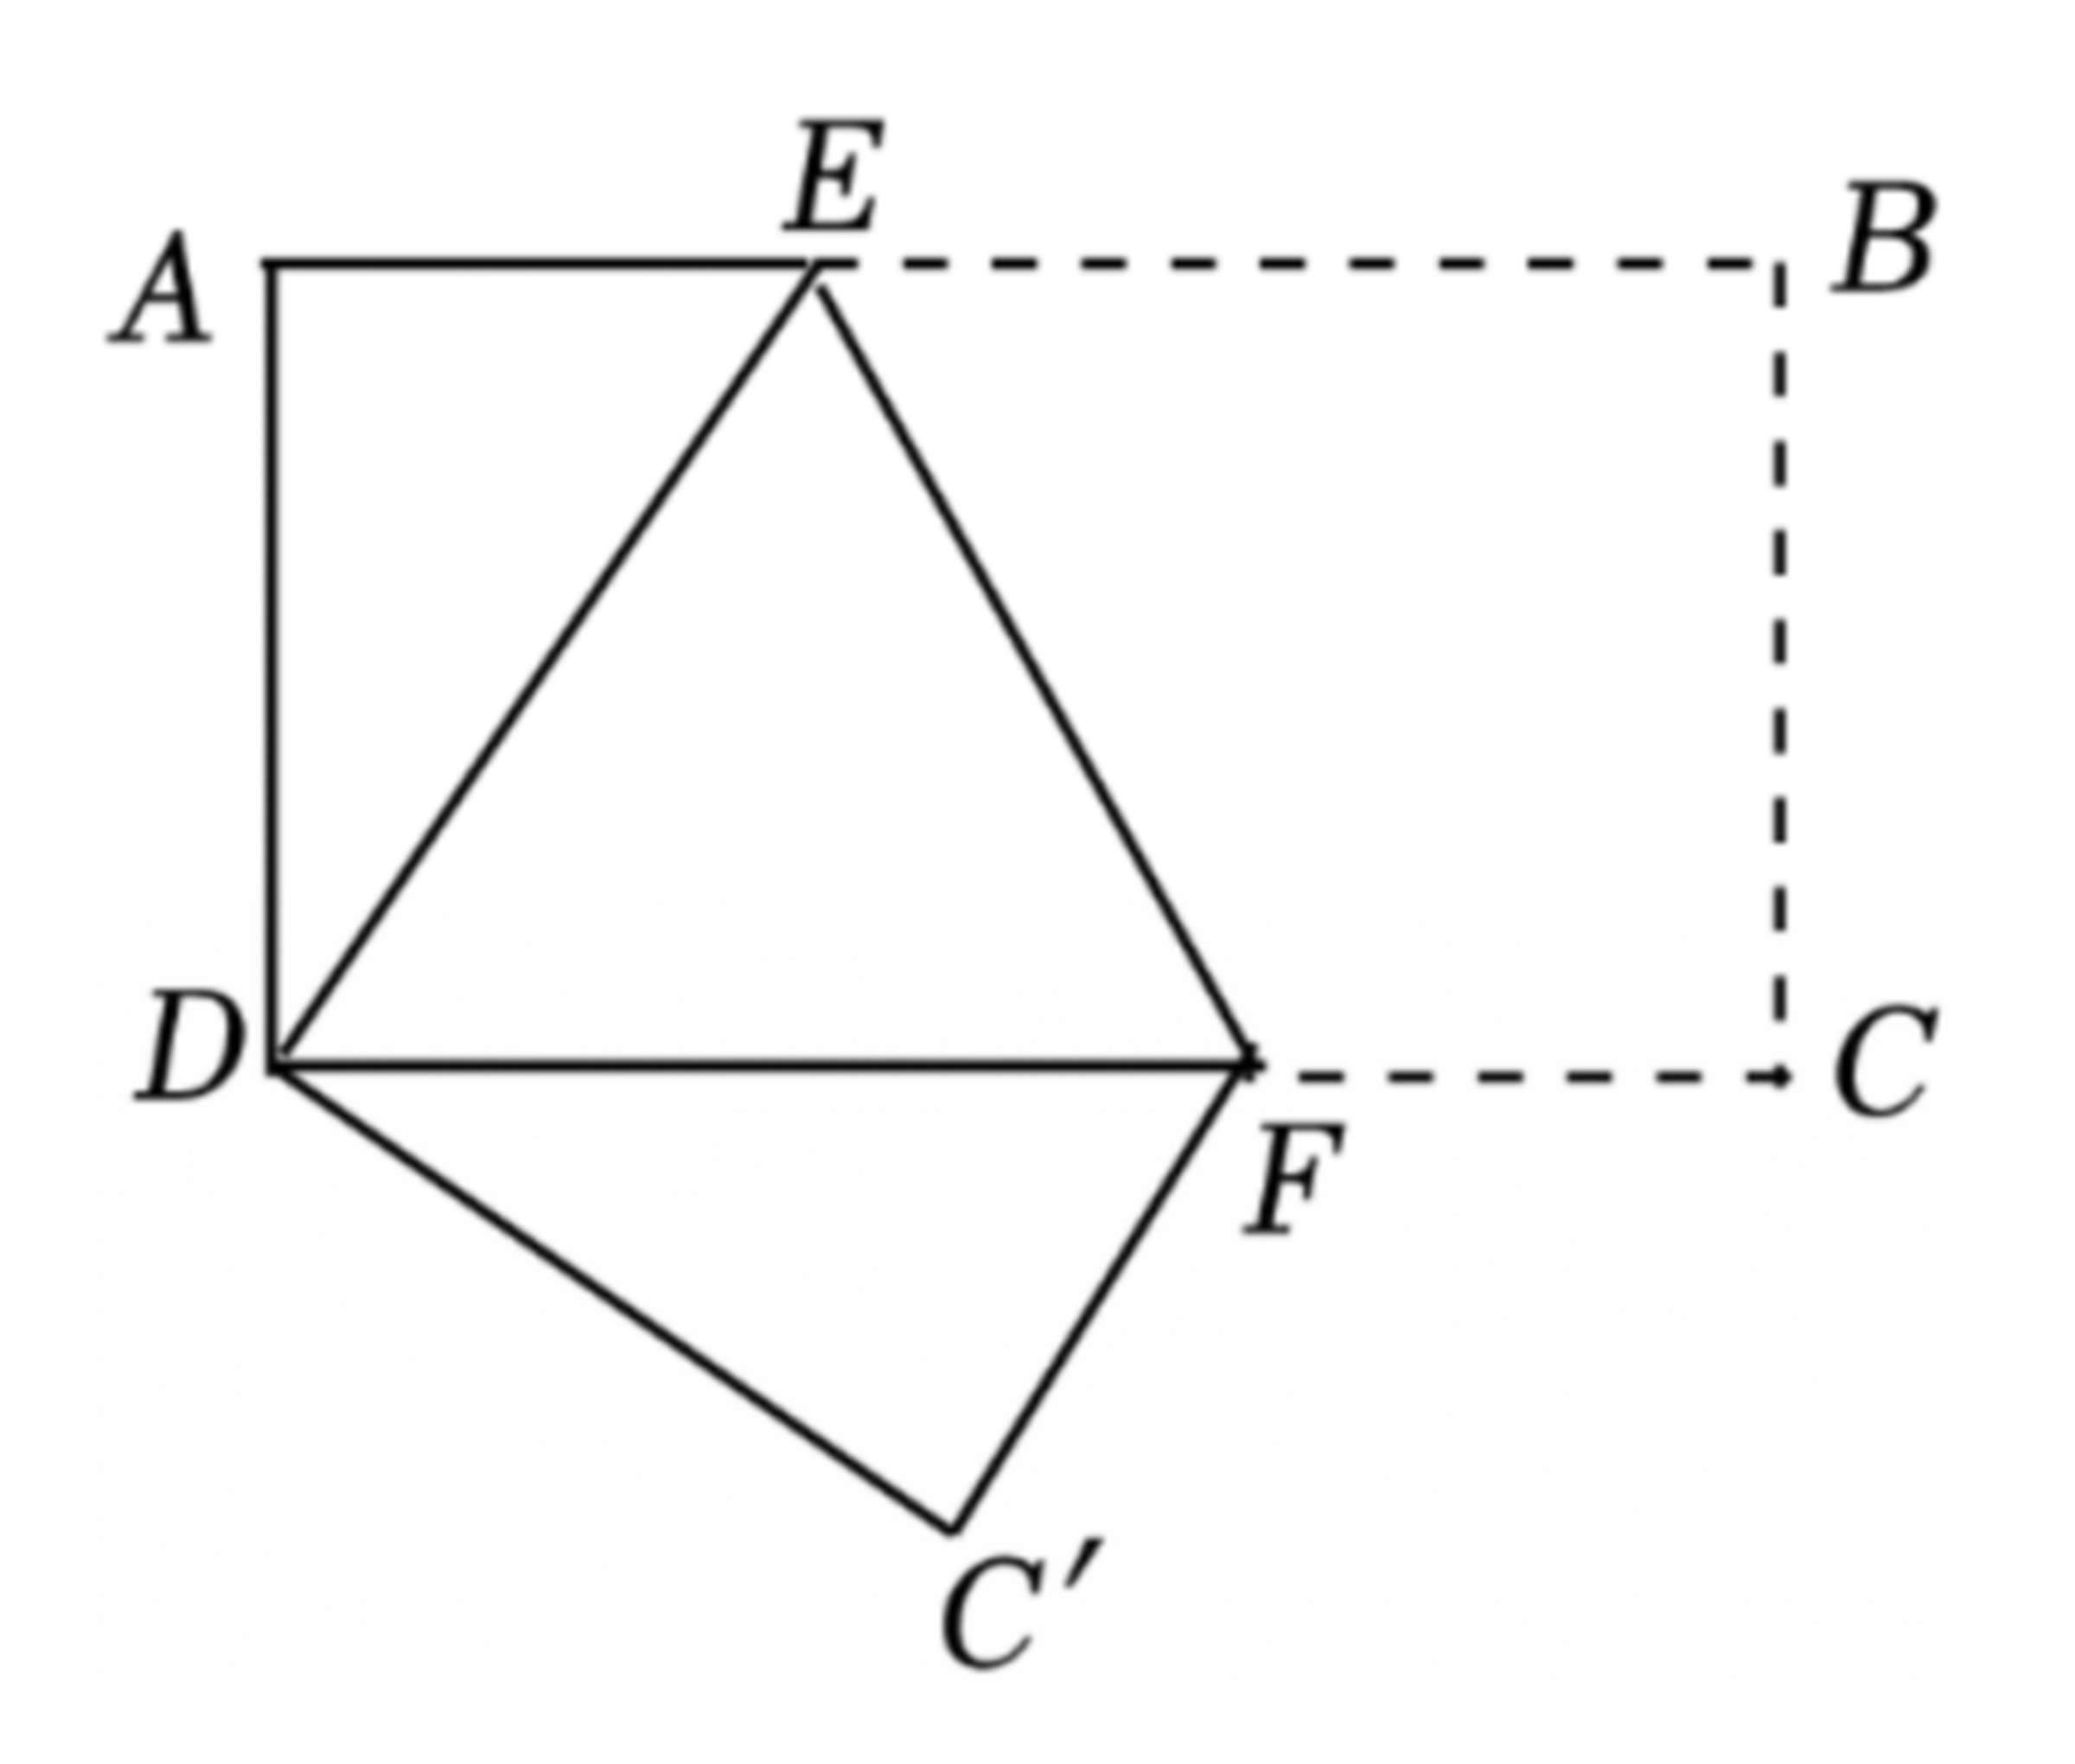
\includegraphics[width=0.40\textwidth]{figures/gao149_q11.png}
\end{center}

\ifanswer
\solbegin
\step{因为矩形 $ABCD(AB>AD)$ 的周长为 12，}
\step{在 $AB$ 和 $CD$ 边上分别取点 $E$ 和 $F$，将四边形 $BCFE$ 沿 $EF$ 折叠，}
\step{使点 $B$ 与点 $D$ 重合，此时点 $C$ 的对应点为 $C'$，}
\step{所以设 $AD=a$，$AB=b$，则 $2(a+b)=12$，}
\step{所以 $a+b=6$，且 $AB>AD$，所以 $b>a>0$，}
\step{设 $DF=x$，则 $C'F=b-x$，在 $Rt\triangle DC'F$ 中，$DC'=BC=a$，}% 几何三角形符号原卷印扁等边细线三角 $\triangle$，照录（放大 02 页确认）；$Rt$ 照录
\step{所以 $a^2+(b-x)^2=x^2$，解得 $x=\dfrac{a^2+b^2}{2b}$，}
\step{因此 $\triangle C'DF$ 的面积 $S=\dfrac{1}{2}\cdot DC'\cdot C'F=\dfrac{1}{2}\cdot a\cdot(b-x)$，}
\step{又 $b-x=b-\dfrac{(6-b)^2+b^2}{2b}=\dfrac{6(b-3)}{b}$，}
\step{所以 $S=\dfrac{1}{2}\cdot a\cdot\dfrac{6(b-3)}{b}=\dfrac{1}{2}\cdot(6-b)\cdot\dfrac{6(b-3)}{b}=\dfrac{3(6-b)(b-3)}{b}$}
\step{$=3\cdot\left(-b-\dfrac{18}{b}+9\right)$，又 $b+\dfrac{18}{b}\geqslant2\sqrt{b\cdot\dfrac{18}{b}}=6\sqrt{2}$，}
\step{当且仅当 $b=\dfrac{18}{b}$ 即 $b=3\sqrt{2}$ 时取等号，此时满足 $b>a$，}
\step{所以 $S\leqslant3\cdot(-6\sqrt{2}+9)=27-18\sqrt{2}$，故 $\triangle C'DF$ 面积的最大值为 $27-18\sqrt{2}$.}
\solend
\fi

% === Q12 === 解析内 3 幅三次函数曲线坐标图（仅答案版出）；解析 15 行（8 行 03 页＋7 行 04 页）
\item 已知 $m>0$，若存在 $t\in\R$，使得对任意 $x\in[0,m]$，不等式 $[(x-1)^2-t](x-t)\leqslant0$ 恒成立，则 $m$ 的最大值是\blankline[4.4em].

\ifanswer
\solbegin
\step{当 $t\leqslant0$ 时，$(x-1)^2-t\geqslant0$ 恒成立，}
\step{不等式 $[(x-1)^2-t](x-t)\leqslant0$ 的解集为 $x\leqslant t$，与 $x\in[0,m]$ 矛盾；}
\step{当 $t>0$ 时，不等式 $[(x-1)^2-t](x-t)\leqslant0\Leftrightarrow(x-1-\sqrt t)(x-1+\sqrt t)(x-t)\leqslant0$，}
\step{若 $t<1-\sqrt t$，即 $t\in\left(0,\dfrac{3-\sqrt5}{2}\right)$，}
\begin{center}
% 情形一 $t<1-\sqrt t$ 曲线图取 03 页右侧，去粉色水印、去色、4× LANCZOS 放大；仅答案版出
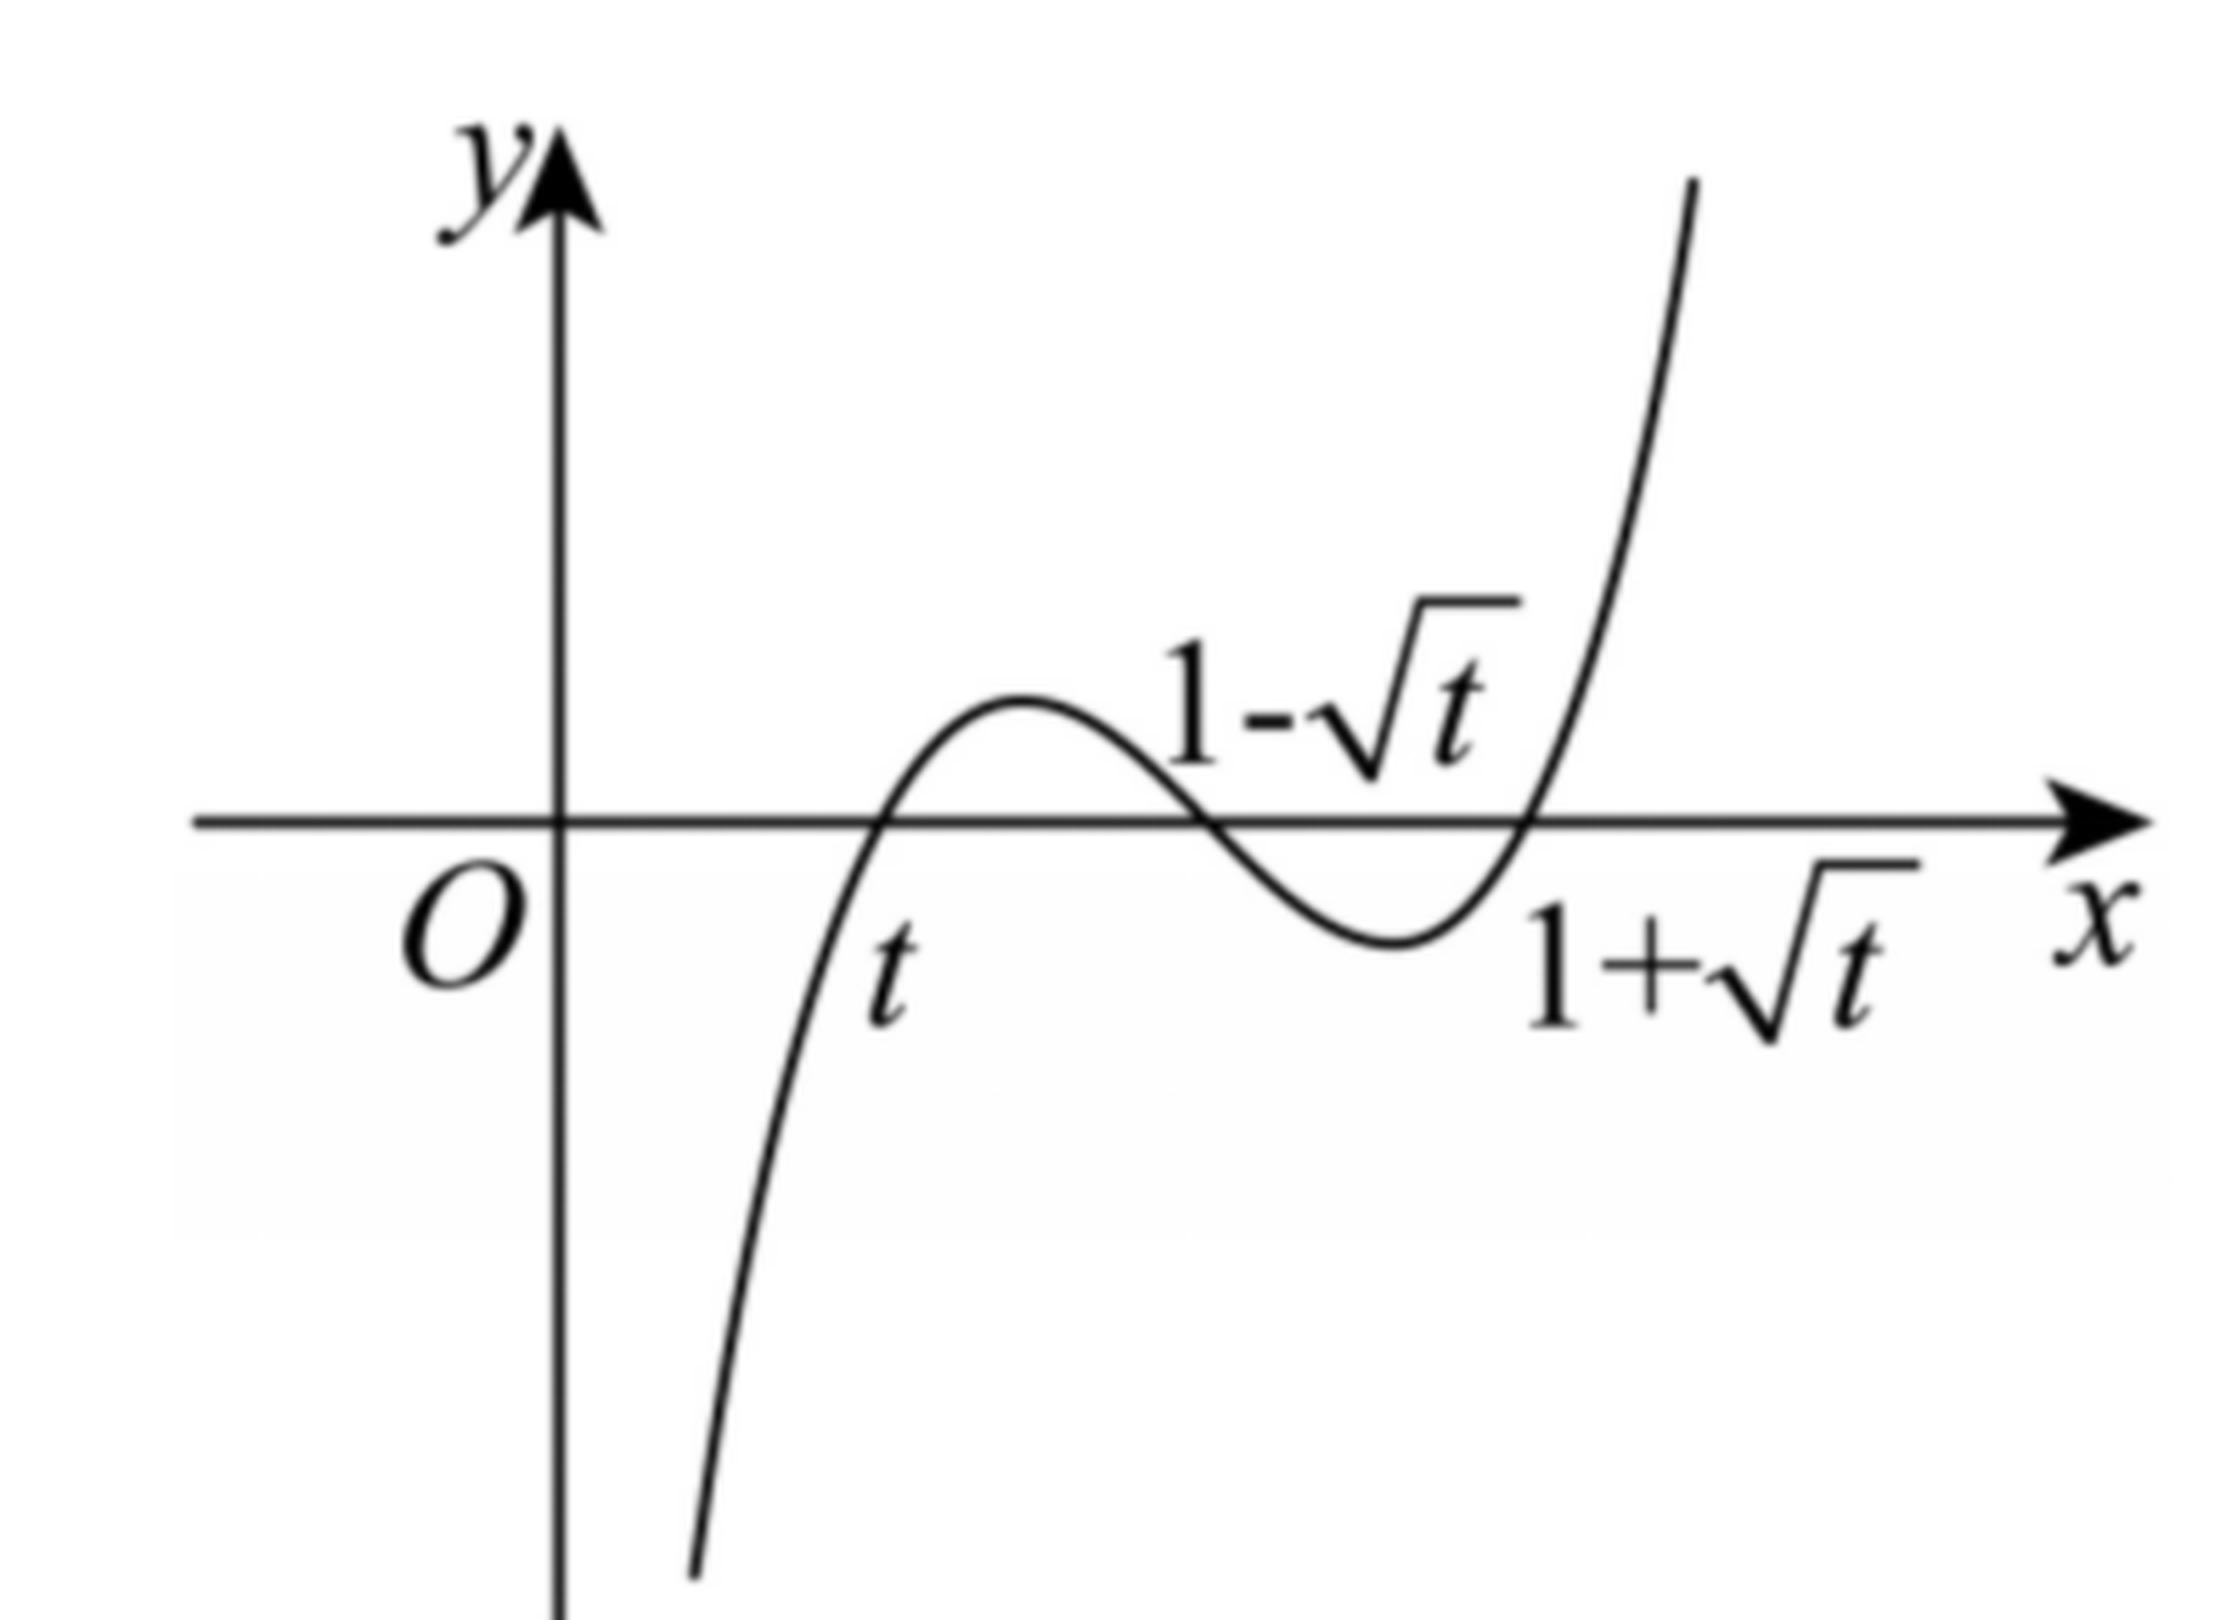
\includegraphics[width=0.40\textwidth]{figures/gao149_q12_a.png}
\end{center}
\step{则原不等式的解集为 $(-\infty,t]\cup[1-\sqrt t,1+\sqrt t]$，}
\step{当 $0<m\leqslant t$ 时，原不等式恒成立，因此}
\step{$m\in\left(0,\dfrac{3-\sqrt5}{2}\right)$；}
\step{若 $t=1-\sqrt t$，即 $t=\dfrac{3-\sqrt5}{2}$，则原不等式的解集为 $(-\infty,1+\sqrt t]$，}
\begin{center}
% 情形二 $t=1-\sqrt t$ 曲线图取 03 页右侧，去粉色水印、去色、4× LANCZOS 放大；仅答案版出
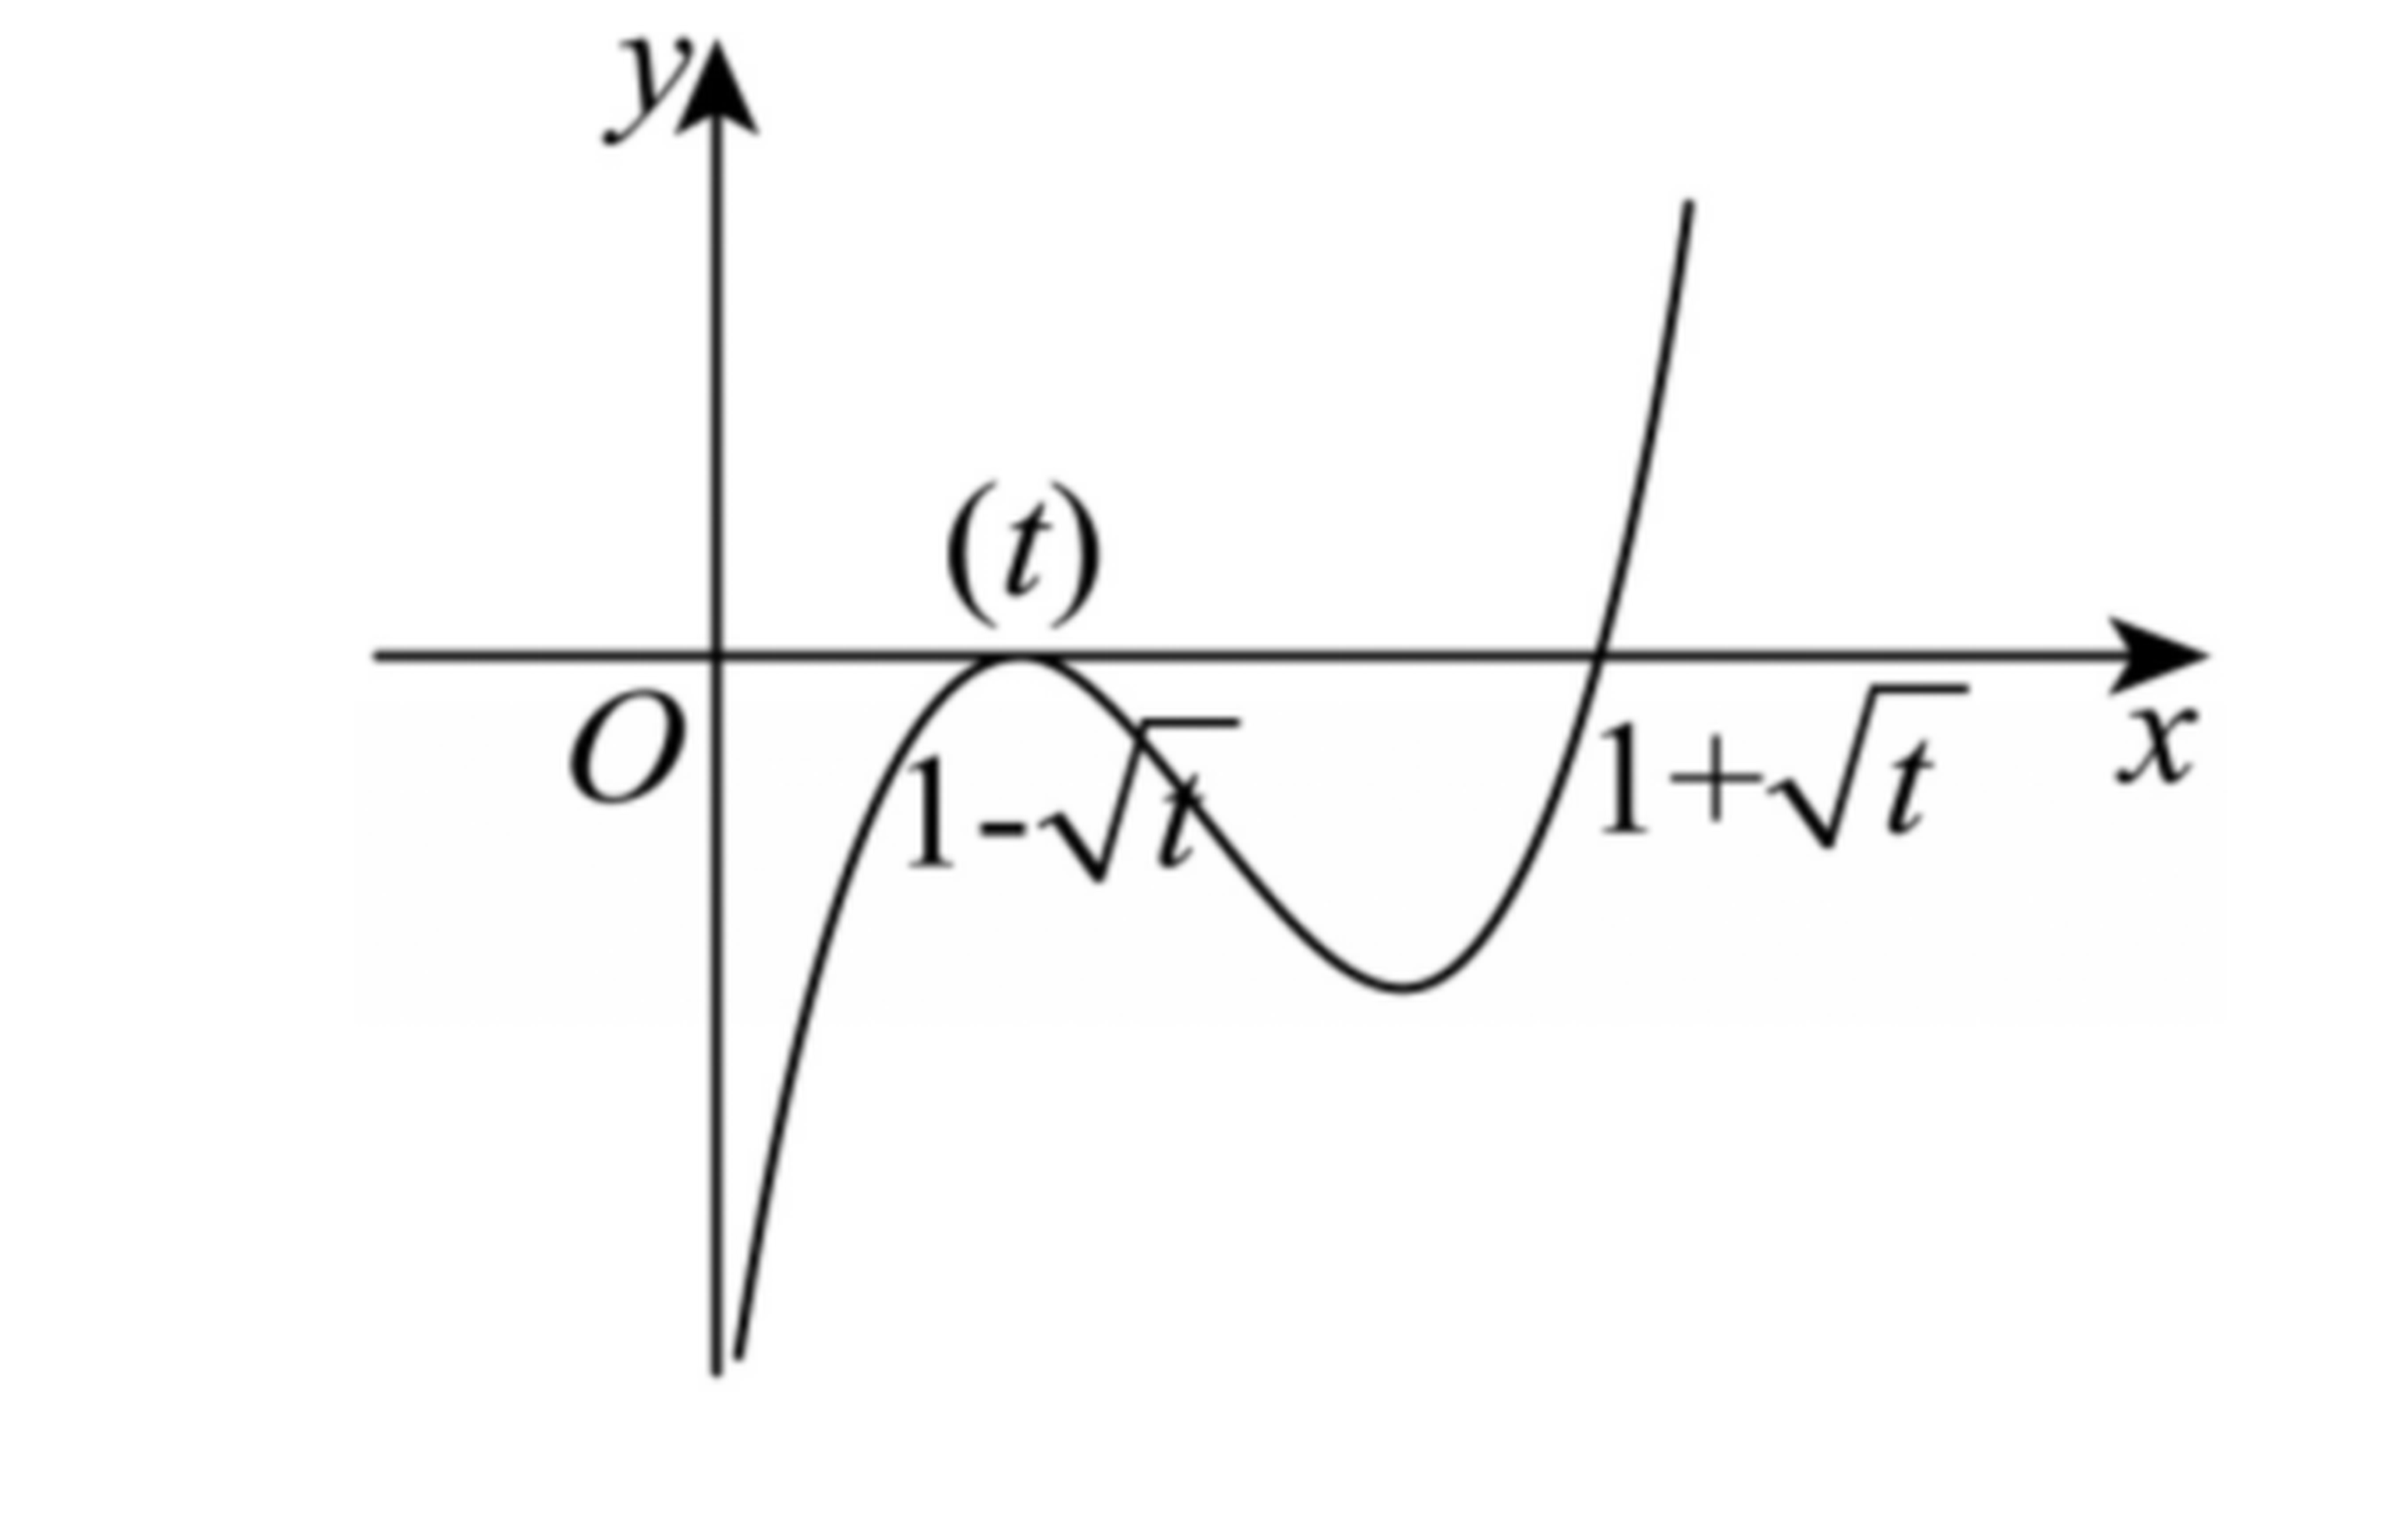
\includegraphics[width=0.40\textwidth]{figures/gao149_q12_b.png}
\end{center}
\step{当 $0<m\leqslant1+\sqrt t$ 时，原不等式恒成立，因此 $m\in\left(0,\dfrac{\sqrt5+1}{2}\right]$；}
\step{若 $1+\sqrt t>t>1-\sqrt t$，即 $t\in\left(\dfrac{3-\sqrt5}{2},\dfrac{3+\sqrt5}{2}\right)$，}
\begin{center}
% 情形三 $1+\sqrt t>t>1-\sqrt t$ 曲线图取 04 页右侧，去粉色水印、去色、4× LANCZOS 放大；仅答案版出
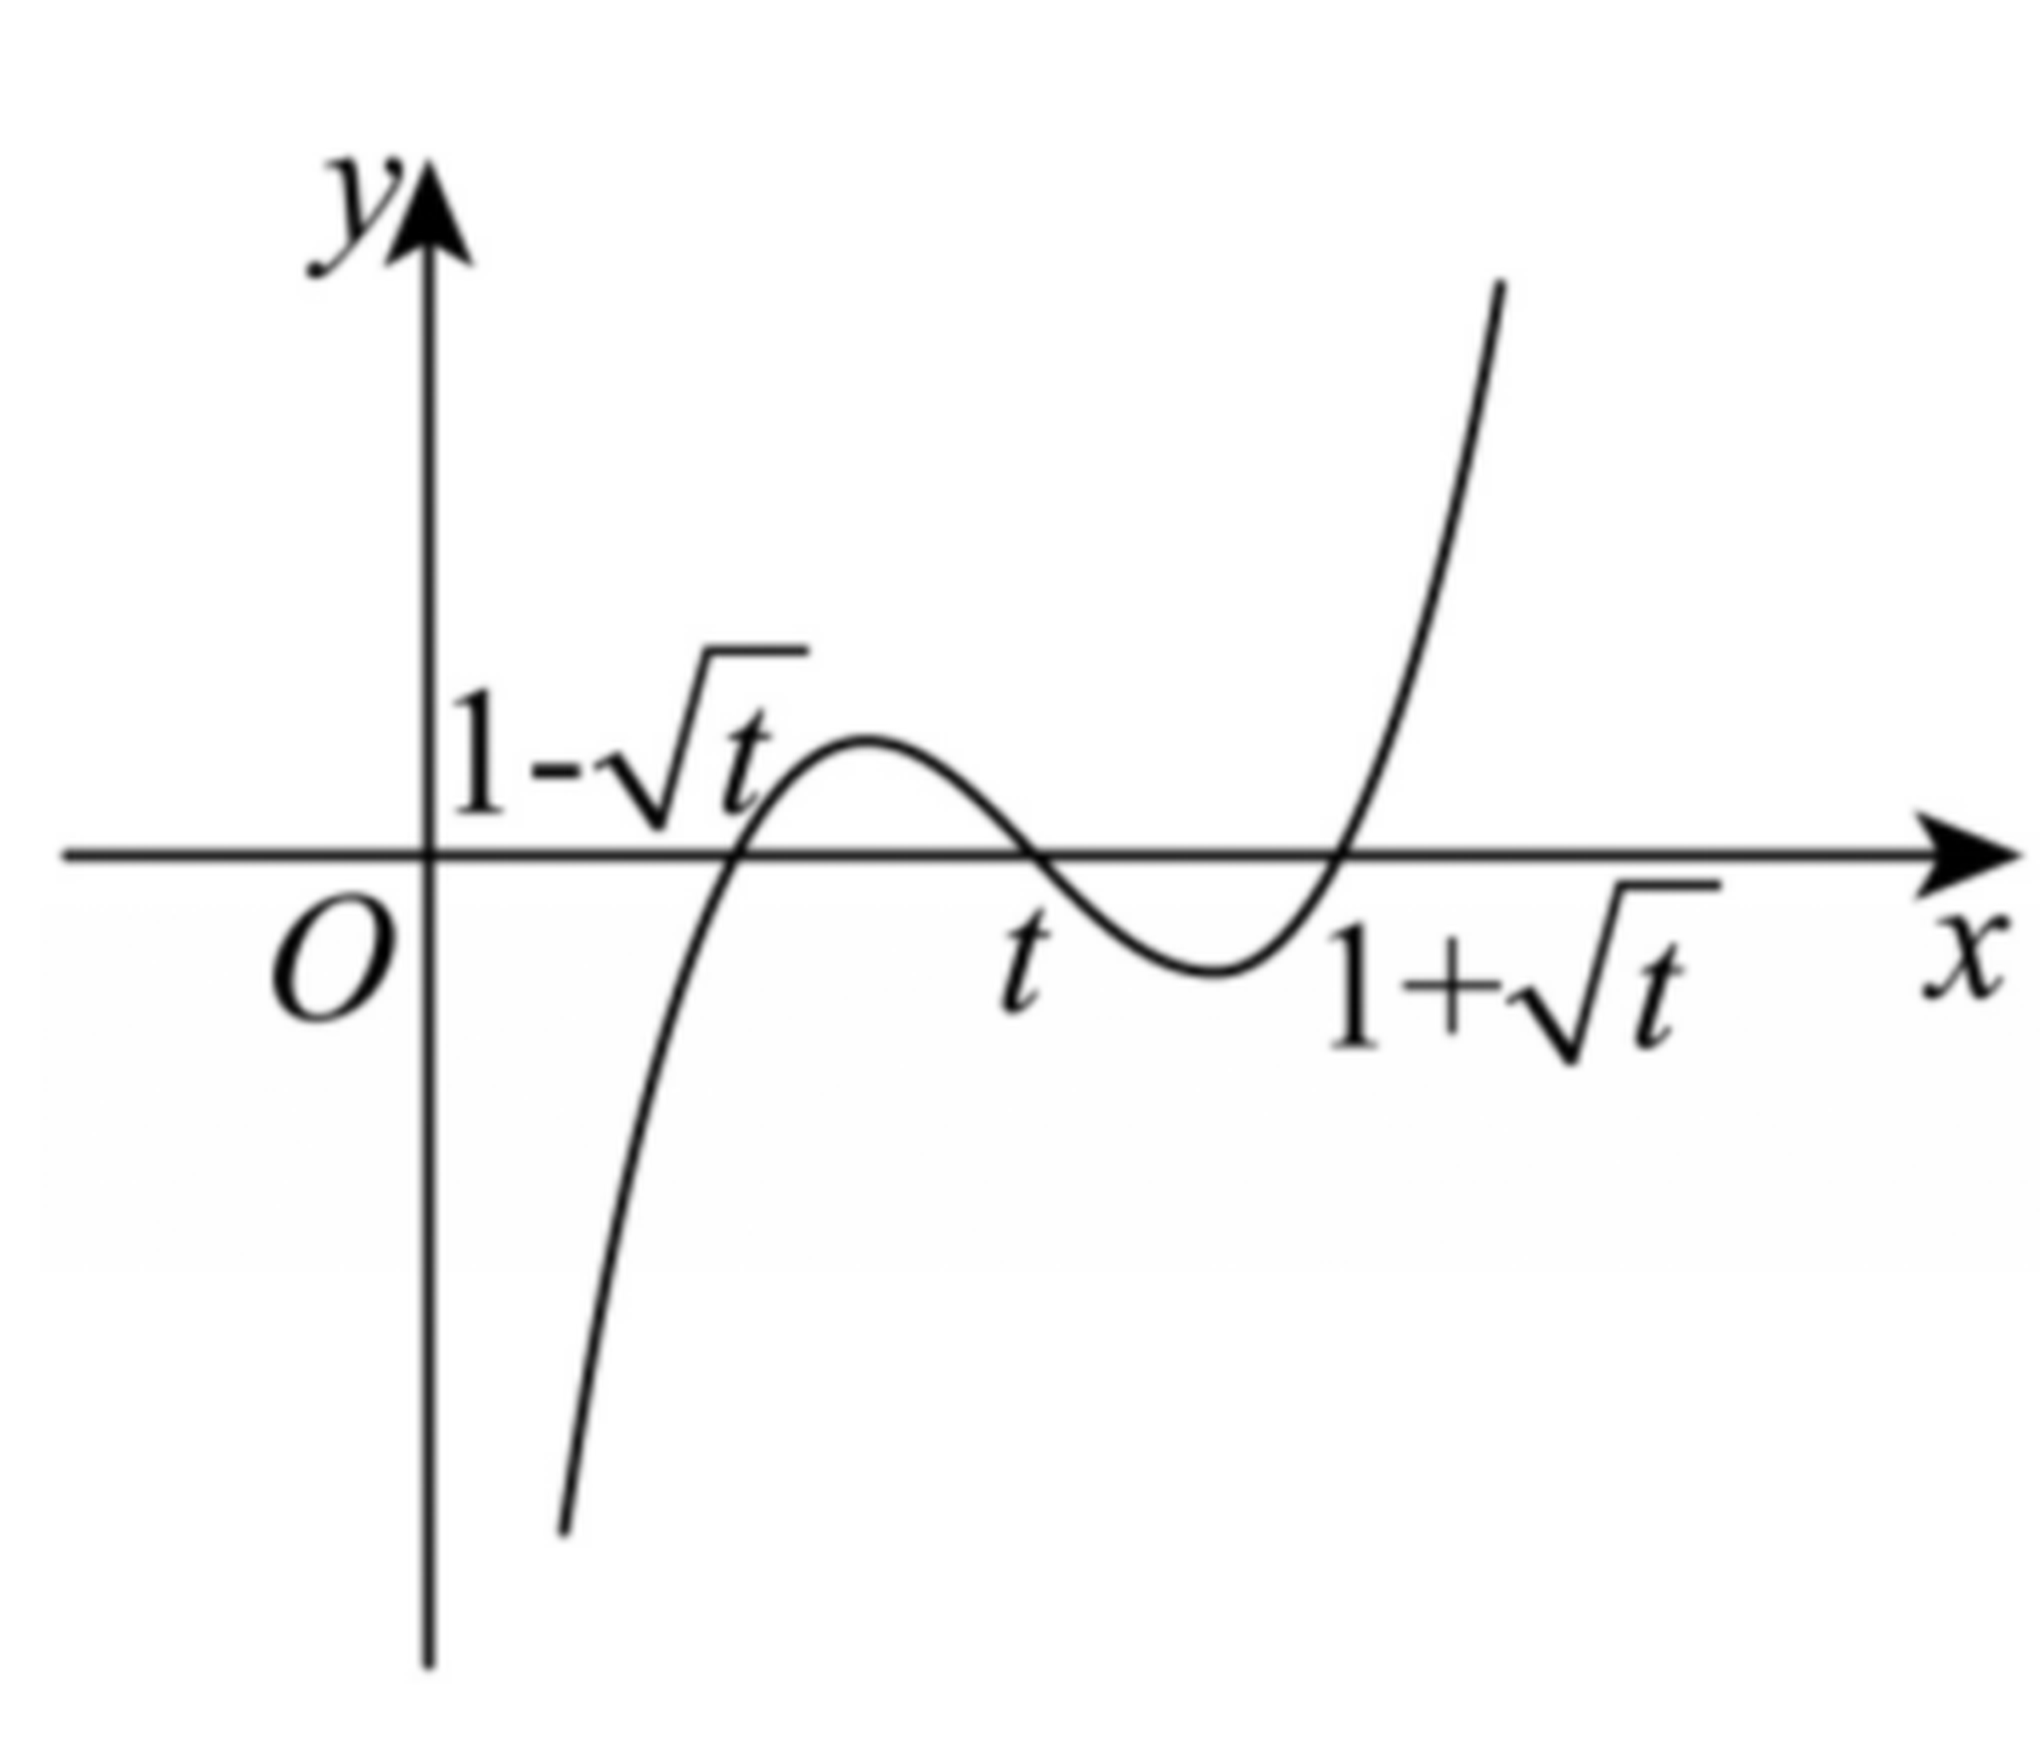
\includegraphics[width=0.40\textwidth]{figures/gao149_q12_c.png}
\end{center}
\step{则原不等式的解集为 $(-\infty,1-\sqrt t]\cup[t,1+\sqrt t]$，}
\step{当 $\begin{cases}1-\sqrt t>0\\1-\sqrt t\geqslant m\end{cases}$ 时，原不等式恒成立，此时 $t\in\left(\dfrac{3-\sqrt5}{2},1\right)$，$m\in\left(0,\dfrac{3-\sqrt5}{2}\right)$；}
\step{若 $t\geqslant1+\sqrt t$，即 $t\geqslant\dfrac{3+\sqrt5}{2}$，则取 $x=0$，$(t-1)t>0$，}
\step{原不等式不恒成立，不符合题意，}
\step{因此实数 $m$ 的取值范围是 $\left(0,\dfrac{\sqrt5+1}{2}\right]$，$m$ 的最大值是 $\dfrac{\sqrt5+1}{2}$.}
\solend
\fi

\end{enumerate}

\bigsec{二、选择题}

\begin{enumerate}
\setcounter{enumi}{12}

% === Q13 ===：答案"C"直接印在题干括号内、无【答案】/【解析】段，按 高一84 Q13／高一148 Q13 成例括号留空、另提 \ans{$C$}；四选项两行两列照原卷分行
\item 设 $ab>0$，则 $a>b$ 是 $\dfrac{1}{a}<\dfrac{1}{b}$ 的\mbox{（\quad）}

\keepwithprev
A. 充分不必要条件\qquad\qquad B. 必要不充分条件

C. 充要条件\qquad\qquad D. 既不充分又不必要条件

\ifanswer
\ans{$C$}
\fi

% === Q14 ===：$A\subset B$ 单线照录；四选项补集照原卷上划线 \overline{A}／\overline{B}；解析 1 行（由韦恩图得 B 对）
\item 已知集合 $A$、$B$ 非空，且 $A\subset B$，则下列式子中一定是空集的为\mbox{（\quad）}

\keepwithprev
A. $\overline{A}\cap B$\qquad B. $A\cap\overline{B}$\qquad C. $\overline{A}\cap\overline{B}$\qquad D. $\overline{A}\cup\overline{B}$

\ifanswer
\solbegin
\step{由韦恩图得 $B$ 对. 故选 $B$.}
\solend
\fi

% === Q15 ===："天文数字"弯引号照录；解析 2 行（首行在 04 页末、末行续 05 页顶）
\item 历史上数学计算方面的三大发明是阿拉伯数字、十进制和对数，其中对数的发明，大大缩短了计算时间，为人类研究科学和了解自然起了重大作用，对数运算对估算“天文数字”具有独特的优势. $2.5^{1000}$ 的估算值约为\mbox{（\quad）}

\keepwithprev
A. $10^{365}$\qquad B. $10^{379}$\qquad C. $10^{389}$\qquad D. $10^{398}$

\ifanswer
\solbegin
\step{$\lg 2.5^{1000}=1000\lg 2.5=1000(1-2\lg 2)\approx1000\times(1-0.602)=398$，}
\step{所以 $2.5^{1000}\approx10^{398}$. 故选 $D$.}
\solend
\fi

% === Q16 ===："完美集"新定义、圈数字①②文本模式；题干"若对任意 $x$，$y\in A$"用全角逗号、解析用顿号"$x$、$y\in A$"，两处照录不统一；解析 9 行
\item 设全集 $U=\R$，集合 $A$ 是一个非空数集，若对任意 $x$，$y\in A$，都有 $x+y\in A$、$xy\in A$，则称集合 $A$ 为一个“完美集”，给出以下命题：

①若 $A_1$、$A_2$ 都是“完美集”，且 $A_1\cap A_2\ne\varnothing$，则 $A_1\cap A_2$ 也是“完美集”；

②若 $A_1$、$A_2$ 都是“完美集”，则 $A_1\cup A_2$ 也是“完美集”.

下列说法正确的是\mbox{（\quad）}

\keepwithprev
A. ①②都是真命题\qquad\qquad B. ①是真命题，②是假命题

C. ①是假命题，②是真命题\qquad\qquad D. ①②都是假命题

\ifanswer
\solbegin
\step{由题意，全集 $U=\R$，集合 $A$ 是一个非空数集，}
\step{若对任意 $x$、$y\in A$，都有 $x+y\in A$、$xy\in A$，则称集合 $A$ 为一个“完美集”，}
\step{对于①，取 $x$、$y\in A_1\cap A_2$，则 $x\in A_1$，$x\in A_2$，$y\in A_1$，$y\in A_2$，}
\step{又 $A_1$、$A_2$ 是“完美集”，所以 $x+y\in A_1$，$xy\in A_1$，$x+y\in A_2$，$xy\in A_2$，}
\step{所以 $x+y\in A_1\cap A_2$，$xy\in A_1\cap A_2$，所以 $A_1\cap A_2$ 是“完美集”，故①正确；}
\step{对于②，取“完美集” $A_1=\{x\mid x=2k,k\in\Z\}$，$A_2=\{x\mid x=3k,k\in\Z\}$，}
\step{则 $2\in A_1$，$3\in A_2$，但 $2+3\notin A_1\cup A_2$，}
\step{即此时 $A_1\cup A_2$ 不是“完美集”，故②错误.}
\step{故选 $B$.}
\solend
\fi
\end{enumerate}

\bigsec{三、解答题}

\begin{enumerate}
\setcounter{enumi}{16}

% === Q17 ===："图像"（有亻）照录（Q17 题干与解析共 2 处）；绝对值 \lvert…\rvert；解析 7 行
\item 已知 $m\in\R$，$f(x)=(m^2-m-5)x^m$. 若 $y=f(x)$ 是幂函数，且其图像不经过原点.

(1) 求实数 $m$ 的值；

(2) 若 $f(a)=f(b)$ 且 $a\ne b$，求 $\lvert a+2\rvert+\lvert b-1\rvert$ 的最小值，并指出取到最小值时 $a$ 的取值范围.

\ifanswer
\solbegin
\step{(1) $f(x)=(m^2-m-5)x^m$ 是幂函数，得 $m^2-m-5=1$，即 $m^2-m-6=0$，}
\step{解得 $m=-2$ 或 $m=3$，又函数图像不经过原点，所以 $m=-2$($3$ 舍)；}
\step{(2) 由 (1) 得 $f(x)=x^{-2}=\dfrac{1}{x^2}$ 为偶函数，}
\step{$x<0$ 时，函数 $f(x)$ 严格增，$x>0$ 时，函数 $f(x)$ 严格减，}
\step{又 $f(a)=f(b)$ 且 $a\ne b$，所以 $a=-b$，且 $a\ne0$，$b\ne0$，}
\step{则 $\lvert a+2\rvert+\lvert b-1\rvert=\lvert a+2\rvert+\lvert-a-1\rvert=\lvert a+2\rvert+\lvert a+1\rvert$，}
\step{则 $\lvert a+2\rvert+\lvert b-1\rvert$ 的最小值为 $1$，取到最小值时 $a$ 的取值范围是 $[-2,-1]$.}
\solend
\fi

% === Q18 ===：判别式两形混用——(1) cases 块印高 \Delta、(2) 独立行印扁 \triangle，逐处照录不统一；解析 8 行
\item 已知命题 $p$：方程 $x^2+4x+m-1=0$ 有两个不等的负根；命题 $q$：方程 $4x^2+4x+m-2=0$ 无实根.

(1) 若 $p$ 为真命题，求 $m$ 的取值范围；

(2) 若 $p$、$q$ 两命题一真一假，求 $m$ 的取值范围.

\ifanswer
\solbegin
\step{(1) 若 $p$ 为真命题，即方程 $x^2+4x+m-1=0$ 有两个不等的负根；}
\step{必有 $\begin{cases}\Delta=16-4(m-1)>0\\m-1>0\end{cases}$，解得 $1<m<5$，即 $m$ 的取值范围为 $(1,5)$；}
\step{(2) 命题 $q$：方程 $4x^2+4x+m-2=0$ 无实根，}
\step{则有 $\triangle=16-16(m-2)<0$，解得 $m>3$，}
\step{若 $p$ 和 $q$ 有且只有一个为真命题，}
\step{若 $p$ 真 $q$ 假，必有 $\begin{cases}1<m<5\\m\leqslant3\end{cases}$，则有 $1<m\leqslant3$，}
\step{若 $p$ 假 $q$ 真，必有 $\begin{cases}m\leqslant1\text{ 或 }m\geqslant5\\m>3\end{cases}$，则有 $m\geqslant5$，}
\step{综上，$1<m\leqslant3$ 或 $m\geqslant5$.}
\solend
\fi

% === Q19 ===：$A\subseteq B$ 带下划线照录；解析 7 行（(2) 两组 cases 并排）
\item 已知 $m\in\R$，集合 $A=\left\{x\mid y=\sqrt{3-x}-\dfrac{1}{\sqrt{x-1}}\right\}$，集合 $B=\{x\mid 2m\leqslant x\leqslant1-m\}$.

(1) 若 $A\cup B=B$，求实数 $m$ 的取值范围；

(2) 若 $A\cap B=\varnothing$，求实数 $m$ 的取值范围.

\ifanswer
\solbegin
\step{(1) 函数 $y=\sqrt{3-x}-\dfrac{1}{\sqrt{x-1}}$，则 $\begin{cases}3-x\geqslant0\\x-1>0\end{cases}$，解得 $1<x\leqslant3$，}
\step{所以 $A=\{x\mid1<x\leqslant3\}$，}
\step{因为 $A\cup B=B$，所以 $A\subseteq B$，则 $\begin{cases}2m\leqslant1\\1-m\geqslant3\end{cases}$，解得 $m\leqslant-2$，}
\step{综上，实数 $m$ 的取值范围为 $(-\infty,-2]$；}
\step{(2) 当 $B=\varnothing$ 时，则 $2m>1-m$，解得 $m>\dfrac{1}{3}$，}
\step{当 $B\ne\varnothing$ 时，则 $\begin{cases}2m\leqslant1-m\\2m>3\end{cases}$ 或 $\begin{cases}2m\leqslant1-m\\1-m\leqslant1\end{cases}$，解得 $m\in\varnothing$ 或 $0\leqslant m\leqslant\dfrac{1}{3}$，}
\step{综上，实数 $m$ 的取值范围为 $[0,+\infty)$.}
\solend
\fi

% === Q20 ===：n 阶基本不等式推广；(3) 解析含 \overbrace{…}^{k} 上括号；(2) 解析"x=x=x=3(1-x)"三连等系原卷笔误、照录加注（见 ⑤）；解析 14 行
\item 教材中的基本不等式可以推广到 $n$ 阶：$n$ 个正数的算术平均数不小于它们的几何平均数，即对于任意的正数 $a_1$、$a_2$、$\cdots$、$a_n$，有 $\dfrac{a_1+a_2+\cdots+a_n}{n}\geqslant\sqrt[n]{a_1\cdot a_2\cdots a_n}$（$n\in\N$ 且 $n\geqslant2$），且等号当且仅当 $a_1=a_2=\cdots=a_n$ 时成立. 利用此结论解决下列问题：

(1) 若 $x$、$y$、$z>0$，求 $\dfrac{y}{x}+\dfrac{2z}{y}+\dfrac{4x}{z}$ 的最小值；

(2) 已知 $0<x<1$，求 $x^3(1-x)$ 的最大值，并求取得最大值时的 $x$ 的值；

(3) 对任意的正整数 $k$，判断 $\left(1+\dfrac{1}{k}\right)^k$ 与 $\left(1+\dfrac{1}{k+1}\right)^{k+1}$ 的大小关系，并证明.

\ifanswer
\solbegin
\step{(1) 因为 $x$、$y$、$z>0$，有 $\dfrac{y}{x}>0$，$\dfrac{2z}{y}>0$，$\dfrac{4x}{z}>0$}
\step{所以 $\dfrac{y}{x}+\dfrac{2z}{y}+\dfrac{4x}{z}\geqslant3\sqrt[3]{\dfrac{y}{x}\cdot\dfrac{2z}{y}\cdot\dfrac{4x}{z}}=3\sqrt[3]{8}=6$，}
\step{当且仅当 $\dfrac{y}{x}=\dfrac{2z}{y}=\dfrac{4x}{z}$ 时取等号，故 $\dfrac{y}{x}+\dfrac{2z}{y}+\dfrac{4x}{z}$ 的最小值为 $6$.}
\step{(2) 因为 $0<x<1$，所以 $1-x>0$，}
\step{$x^3(1-x)=\dfrac{1}{3}[x\cdot x\cdot x\cdot3(1-x)]\leqslant\dfrac{1}{3}\left[\dfrac{x+x+x+3(1-x)}{4}\right]^4=\dfrac{1}{3}\times\left(\dfrac{3}{4}\right)^4$}
\step{$=\dfrac{27}{256}$，当且仅当 $x=x=x=3(1-x)$，即 $x=3(1-x)$，$x=\dfrac{3}{4}$ 取等号，}% 原卷"x=x=x=3(1-x)"三连等，疑为四因子相等之误排，放大 08 页确认，照录未改（见 ⑤）
\step{所以 $0<x<1$ 时，$x^3(1-x)$ 的最大值是 $\dfrac{27}{256}$，取最大值时 $x=\dfrac{3}{4}$.}
\step{(3) 对任意 $k\in\N^*$，$\left(1+\dfrac{1}{k}\right)^k<\left(1+\dfrac{1}{k+1}\right)^{k+1}$.}
\step{证明：$\left(1+\dfrac{1}{k}\right)^k=\overbrace{\left(1+\dfrac{1}{k}\right)\cdot\left(1+\dfrac{1}{k}\right)\cdots\left(1+\dfrac{1}{k}\right)}^{k}\times1$}
\step{$\leqslant\left(\dfrac{\overbrace{\left(1+\dfrac{1}{k}\right)+\left(1+\dfrac{1}{k}\right)+\cdots+\left(1+\dfrac{1}{k}\right)}^{k}+1}{k+1}\right)^{k+1}$}
\step{$=\left(\dfrac{\overbrace{(1+1+\cdots+1)}^{k}+\overbrace{\left(\dfrac{1}{k}+\dfrac{1}{k}+\cdots+\dfrac{1}{k}\right)}^{k}+1}{k+1}\right)^{k+1}=\left(\dfrac{k+1+1}{k+1}\right)^{k+1}=\left(1+\dfrac{1}{k+1}\right)^{k+1}$，}
\step{当且仅当 $1+\dfrac{1}{k}=1$ 时取等号，}
\step{但是任意 $k\in\N^*$ 时 $1+\dfrac{1}{k}>1$，所以等号不成立，}
\step{故任意 $k\in\N^*$ 时，$\left(1+\dfrac{1}{k}\right)^k<\left(1+\dfrac{1}{k+1}\right)^{k+1}$.}
\solend
\fi

% === Q21 ===："减 k 集"新定义（引号内 k／数字两侧空格照录）；解析 26 行（续 10 页），含 ⑤ 三处原卷笔误照录
\item 定义：对于给定的整数 $k$，若非空集合 $A$ 满足如下 3 个条件：

① $A$ 是正整数集的子集；② $A\ne\{1\}$；

③对任意正整数 $x,y$，若 $x+y\in A$，则 $xy-k\in A$；则称集合 $A$ 为“减 $k$ 集”.

(1) 判断集合 $A=\{1,2\}$ 是否为“减 $0$ 集”？是否为“减 $1$ 集”？（无需说明理由）

(2) 证明：不存在“减 $2$ 集”；

(3) 是否存在“减 $1$ 集”？如果存在，求出所有“减 $1$ 集”；如果不存在，说明理由.

\ifanswer
\solbegin
\step{(1) 因为 $P\subseteq\N^*$，$P\ne\{1\}$，$1+1=2\in P$，$1\times1-0\in P$，}
\step{所以集合 $P=\{1,2\}$ 是“减 $0$ 集”；}
\step{因为 $P\subseteq\N^*$，$P\ne\{1\}$，$1+1=2\in P$，$1\times1-1\notin P$，}
\step{所以集合 $P=\{1,2\}$ 是“减 $1$ 集”；}% 按条件③应为"不是"，原卷径印"是"，放大 09 页确认，照录未改（见 ⑤）
\step{(2) 假设存在集合 $A$ 是“减 $2$ 集”，若 $x+y\in A$，则 $xy-2\in A$，}
\step{①当 $x+y=xy-2$ 时，有 $(x-1)(y-1)=3$，}
\step{则 $x$、$y$ 一个为 $2$，一个为 $4$，所以集合 $A$ 有元素 $6$，}
\step{但 $3+3\in A$，$3\times3-2\notin A$，与 $A$ 是“减 $2$ 集”矛盾；}
\step{②当 $x+y\ne xy-2$ 时，则 $x+y=xy-1$ 或 $x+y=xy-m$($m>2$)，}
\step{若 $x+y=xy-1$，$m=1$ 时，$M$ 为除 $1$ 以外的最小元素，}% 原卷"m=1"上文未显式定义，疑笔误，放大 09 页确认，照录未改（见 ⑤）
\step{则 $x=M-1$，$y=1$ 时，$xy-2=M-3$ 小于 $M$，}
\step{要符合题意，必须 $M=4$，}
\step{此时取 $x-2$，$y=2$，$xy-2=2$ 不属于 $A$，故不符合题意，}% 原卷"取 x−2"疑为"取 x=2"误排，放大 09 页确认，照录未改（见 ⑤）
\step{当 $m>2$ 时，$(x-1)(y-1)=m+1$，同样得出矛盾，}
\step{综上，不存在 $A$ 是“减 $2$ 集”.}
\step{(3) 存在“减 $1$ 集” $A$，则 $A\ne\{1\}$，}
\step{①假设 $1\in A$，则 $A$ 中除了元素 $1$ 以外，必然还含有其它元素，}
\step{假设 $2\in A$，$1+1\in A$，而 $1\times1-1\notin A$，所以 $2\notin A$，}
\step{假设 $3\in A$，$1+2\in A$，而 $1\times2-1\in A$，所以 $3\in A$，}
\step{所以 $A=\{1,3\}$，}
\step{假设 $4\in A$，$1+3\in A$，而 $1\times3-1\notin A$，所以 $4\notin A$，}
\step{假设 $5\in A$，$1+4\in A$，$1\times4-1\in A$，$2+3=5$，$2\times3-1\in A$，所以 $5\in A$，}
\step{所以 $A=\{1,3,5\}$，}
\step{以此类推，得 $A=\{1,3,5,\cdots,2n-1,\cdots\}$，($n\in\N^*$)，}
\step{所以所有的“减 $1$ 集”有 $\{1,3\}$，$\{1,3,5\}$，$\{1,3,5,7\}$，$\cdots$，$\{1,3,5,\cdots,2n-1,\cdots\}$，}
\step{$(n\in\N^*)$.}
\solend
\fi
\end{enumerate}

\end{document}
"
%
% ① 原始材料：微信公众号"魔都数学加油站"文章，连载"27学年高一149"，原文标题
% "27学年高一149——2026-2027年上海市青浦高级中学上外云间高一上期中"；
% 原文链接：https://mp.weixin.qq.com/s/T7_nyoR1k0o_5og7FkDsyw 。
% 正文为 10 张 PNG 页（01/02/03/04/10 为 2560×3620，05/06/07/08/09 为 4762×6735，
% 同一篇各页分辨率混排，逐页按各自分辨率裁图核对，别按预览比例换算裁框）。
% 体例：混合体例讲评版——19 题中 Q6 只印【答案】、无【解析】；Q13 的答案"C"
%   直接印在题干括号内、无【答案】/【解析】段；其余 17 题印【解析】（逐题核实，见 ② ②）。
% 题目、答案、解析均据原图转录；卷面粉红色水印"魔都数学加油站"及公众号页脚未录入。
% 全卷插图清单（逐页通读 10 页确认）：1 幅题目配图 + 3 幅【解析】内配图：
%   · Q11 矩形 ABCD 折叠几何图（02 页右侧：A/B/C/D/E/F/C' 与虚线 EB、BC、FC），
%     题干"如图"处，题目配图、三版都出，裁 figures/gao149_q11.png；
%   · Q12【解析】内 3 幅三次函数曲线坐标图（03 页右侧两幅 + 04 页右侧一幅：
%     x/y 轴、O、t、1-\sqrt t、1+\sqrt t 等标注，分别对应 t<1-\sqrt t、
%     t=1-\sqrt t、1+\sqrt t>t>1-\sqrt t 三种情形），解析配图、仅答案版出，
%     分别裁 figures/gao149_q12_a.png／_b.png／_c.png，放 \ifanswer 内 \step 之间
%     （高一73 第 16 题成例）；
%   其余各页逐页确认无其它题目配图、无表格；Q14 解析"由韦恩图得 B 对"仅文字推导、
%   原卷并未印韦恩图；Q9／Q18／Q19 的 cases 块与 Q20(3) 的 \overbrace 为数学块（非图）；
%   10 页下半仅水印、无正文。4 图均取自原卷截图，去粉色水印、去色、4× LANCZOS 放大。
%
% 卷首标题：原卷印作"2026-2027 年青浦高级中学上外云间高一上期中"，年份区间按全稿
% 惯例排 en dash；原卷卷面未印副标题，本稿按同期中卷（高一140／141／143／144／145／
% 146／147／148）知识模块口径补出"集合与常用逻辑用语、不等式、函数"。
%
% 题号体例（逐页核实定稿）：本卷共 19 题——一、填空题 3—12（10 题）、
% 二、选择题 13—16（4 题）、三、解答题 17—21（5 题）。
% 三节分别 \setcounter{enumi}{2}／{12}／{16}。原卷从第 3 题起、无第 1、2 题，
% 本稿保留原题号；全卷无附加题节（Q21 解析末行"（n\in N^*）."为全卷收尾）。
%
% ② 与原卷的排版差异：
%   ① 原文从第 3 题起，本稿保留原题号；共 19 题三节；
%   ② 混合体例逐题核实：Q6（反证法"假设的内容"）只印【答案】、无【解析】，
%      按 高一140 第 5 题／高一145 Q3 成例提 \ans{}、不补造解析；Q13 答案"C"直接
%      印在题干括号内、全卷无该题【答案】/【解析】段，按 高一84 Q13／高一148 Q13
%      成例括号 \mbox{（\quad）} 留空、另提 \ans{$C$}；其余 17 题印【解析】、
%      用 \solbegin…\solend，选择题答案在解析末句"故选 X"（Q14 选 B、Q15 选 D、
%      Q16 选 B，逐个放大 04/05 页核实）、题干括号留空、不另提 \ans{}；
%      答案版【答案】/【解析】标记数 = 19（2 个 \ans ＋ 17 个 \solbegin）
%      = 全卷题数；
%   ③ 原卷卷面未印副标题，本稿按知识模块口径补出；
%   ④ 原卷填空横线按全稿惯例排 \blankline[4.4em]；选择题括号排 \mbox{（\quad）}、
%      选项段前按惯例加 \keepwithprev；Q13／Q16 四选项为两行两列、Q14／Q15
%      选项为一行，照原卷分行；解答题不留作答区、不加 \anspace（原卷为讲评版）；
%   ⑤ 数集：Q6"a,b\in N"、Q8"x\in R"、Q9"a\in R"／"解集为 R"、Q12"t\in R"、
%      Q16"U=R"、Q17"m\in R"、Q19"m\in R"、Q20"n\in N" 原卷印斜体 R/N，
%      按全稿惯例统一改 \R／\N；Q20(3)、Q21 的 $N^*$ 排 \N^*；Q16 解析
%      "$k\in Z$" 排 \Z。绝对值排 \lvert…\rvert（Q17），集合描述竖线排 \mid
%      （Q19、Q16 解析）；不等号按全稿惯例排 \leqslant／\geqslant；
%      补集照原卷上划线排 \overline{A}／\overline{B}（Q14 四选项）；空集
%      \varnothing（Q16、Q19、Q21）；
%   ⑥ 子集符号逐处照录不统一：Q4 题干"{1,2}⊆A⊂{1,2,3,4,5,6}" 前者印带下划线
%      ⊆、照录 \subseteq，后者印单线 ⊂、照录 \subset；Q10"A⊆{-1,1/2,2,3}"、
%      Q19 解析"A⊆B"、Q21 解析"P⊆N*" 均印带下划线 ⊆、照录 \subseteq；
%      Q14"A⊂B" 印单线 ⊂、照录 \subset（逐处放大 01/02/04/07/09 页确认，见 ④）；
%   ⑦ 子题标号 (1)(2)(3) 半角括号照录；圈数字 ①②③ 在文本模式（Q16 两命题、
%      Q21 三个条件与解析的①②）按 common.sty 划入 CJK 字符类渲染；cases 块整体
%      算一个印刷行；\left…\right 不得拆到不同 $…$ 组；数学式内 CJK 用 \text{}
%      （Q18 解析 cases 块"\text{或}"）；Q11 解析"Rt\triangle DC'F" 的 Rt 照录；
%   ⑧ 题干／解析中的中文弯引号按原卷照录：Q6" 已知 a,b\in N，若 ab 能被 5 整除，
%      那么 a、b 中至少有一个能被 5 整除 "（开引号后紧跟"已知"、闭引号后空格接"时"）、
%      Q15"天文数字"、Q16"完美集"、Q21"减 k 集""减 0 集""减 1 集""减 2 集"
%      （引号内 k／数字两侧有空格），注释内一律 ASCII 引号；
%   ⑨ 半角逗号在数学组之间是全稿惯例、非笔误（Q8"$a>0,a\ne1,x\in\R$"、
%      Q21 题干"$x,y$" 等），逐处照录别改；Q16 题干"若对任意 $x$，$y\in A$"
%      用全角逗号而解析用顿号"$x$、$y\in A$"，两处不同均照录；行末西文句点
%      照录为 ASCII `.`；行中全角逗号／顿号照录；
%   ⑩ "图像／图象"逐处放大核：Q10 题干与解析共 6 处均印"图象"（象，无亻）；
%      Q17 题干"其图像不经过原点"与解析"又函数图像不经过原点" 2 处印"图像"
%      （像，有亻），逐处照录未统一改动（放大 02/05/06 页确认）；
%   ⑪ 判别式 Δ/△ 混用是照录项：Q9 解析 cases 块"Δ=4(a−2)²+16(a−2)<0"、
%      Q18(1) cases 块"Δ=16−4(m−1)>0" 两处印等腰偏高粗三角 \Delta；
%      Q18(2) 独立行"△=16−16(m−2)<0" 印扁等边细线三角 \triangle，
%      逐处放大判断、照录不统一（参照 高一142／144／145／146／148 头注④口径）；
%      另 Q11 题干"△C'DF 面积"与解析 3 处"△"（含"Rt△DC'F"）共 4 处几何
%      三角形符号亦印扁细线三角，照录 \triangle（非判别式，字形同类，见 ④）；
%   ⑫ 一条 \step = 原卷解析的一个印刷行，cases 块整体算一个印刷行；别把原卷折行
%      并起来、别把一行拆多条。Q11 十三行（7 行在 02 页＋6 行在 03 页）、
%      Q12 十五行（8 行在 03 页＋7 行在 04 页）、Q16 九行、Q21 二十六行
%      （续 10 页）均按印刷行逐条断，不丢行；
%   ⑬ 配图：Q11 题目配图（三版都出）放 \item 内题干之后 \begin{center}，
%      大图块加 \needvspace{8cm} 守卫把整块推走（守卫放 \item 之前，见
%      高一145 Q14/Q20 成例与切页审计 B 类坑）；Q12 三幅解析配图（仅答案版出）
%      放 \ifanswer 内 \solbegin…\solend 的 \step 之间；三版切页审计均"合计异常：无"；
%   ⑭ 跨页续印按题合并：Q3/4/5 在 01 页；Q6/7/8 题干与解析在 01 页；
%      Q9 题干在 01 页末、解析 4 行在 02 页顶；Q10 题干＋解析在 02 页；
%      Q11 题干＋图＋解析前 7 行在 02 页、解析后 6 行续 03 页顶；
%      Q12 题干＋解析首行在 03 页末、解析续 7 行在 03 页下半＋7 行在 04 页顶，
%      "二、选择题"标题在 04 页下半；Q13/14 题干＋选项＋Q14 解析在 04 页下半；
%      Q15 题干＋选项＋解析首行在 04 页末、末行"所以 2.5^1000≈10^398. 故选 D."
%      续 05 页顶；Q16 题干＋选项＋解析 9 行在 05 页、"三、解答题"标题＋
%      Q17 题干首句在 05 页末；Q17(2)＋解析 7 行、Q18 题干＋解析前 6 行在 06 页；
%      Q18 解析末 2 行续 07 页顶；Q19 题干＋解析 4 行在 07 页上半、
%      解析续 3 行在 07 页下半；Q20 题干(1) 在 07 页末、题干(2)(3)＋解析(1)(2)
%      在 08 页上半、(3) 解析含 \overbrace 的证明在 08 页下半、末行
%      "故任意 k∈N* 时…"续 09 页顶；Q21 题干＋解析(1)(2)(3) 前段在 09 页、
%      解析(3) 后半 9 行续 10 页上半（10 页下半仅水印、无正文）。
%      本稿按题连排，不丢行、不并折行；
%   ⑮ 原卷解析内无红色"法一／法二"之类小标题，故本卷无 \stepm；水印
%      "魔都数学加油站"红色不录入。
%
% ③ 行数复核：一条 \step／\stepm = 原卷解析的一个印刷行，cases 块作一个印刷行计。
%   逐题数（主会话逐页核对定稿）：Q3：1；Q4：2；Q5：2；Q6：0（只印【答案】、
%   提 \ans{}）；Q7：1；Q8：1；Q9：4；Q10：5；Q11：13；Q12：15；
%   Q13：0（答案印在题干括号内、另提 \ans{}）；Q14：1；Q15：2；Q16：9；
%   Q17：7；Q18：8；Q19：7；Q20：14；Q21：26。
%   合计 118 条 \step（本卷无 \stepm：解析内无红色"法一／法二"类小标题），
%   与原卷逐题印刷行相等。全卷 17 题设 \solbegin…\solend ＋ 2 处 \ans{}，
%   答案版【答案】/【解析】标记数 = 19 = 全卷题数。
%
% ④ 判别式／子集符号结论（逐处放大原图照录、不得统一，主会话像素级复核）：
%   判别式全卷 3 处，两形混用逐处照录不统一（参照 高一142／144／145／146／148 头注④）：
%     · Q9 解析 cases 块"Δ=4(a−2)²+16(a−2)<0" 原卷印等腰偏高粗三角（高>宽、
%       粗笔画），照录 \Delta（放大 02 页 /tmp/gao149/z/t02_q9_delta2.png 确认）；
%     · Q18(1) cases 块"Δ=16−4(m−1)>0" 原卷印等腰偏高粗三角（高>宽、粗笔画），
%       照录 \Delta（放大 06 页 /tmp/gao149/z/t06_q18a.png 确认）；
%     · Q18(2) 独立行"△=16−16(m−2)<0" 原卷印扁等边细线三角（宽>高、细线），
%       照录 \triangle（放大 06 页 /tmp/gao149/z/t06_q18b.png 与 Q18(1) 并排确认）。
%   另 Q11 题干"△C'DF"与解析 3 处"△"（含"Rt△DC'F"）共 4 处几何三角形符号
%     亦印扁等边细线三角，照录 \triangle（放大 02 页
%     /tmp/gao149/z/t02_q11_tri2.png 确认），与 Q9／Q18(1) 判别式 \Delta 两形不统一。
%   子集／补集：Q4 题干"{1,2}⊆A⊂{1,2,3,4,5,6}" 前者带下划线 ⊆、照录 \subseteq，
%     后者单线 ⊂、照录 \subset（放大 01 页 /tmp/gao149/z/t01_q3q4.png 确认）；
%     Q10"A⊆{-1,1/2,2,3}"、Q19 解析"A⊆B"、Q21 解析"P⊆N*" 三处带下划线 ⊆、
%     照录 \subseteq；Q14"A⊂B" 单线 ⊂、照录 \subset（放大 04 页
%     /tmp/gao149/z/t04_q14_sub2.png 确认）；Q14 四选项补集 \overline{A}／\overline{B}
%     照原卷上划线；空集 \varnothing（Q16、Q19、Q21）；Q19／Q16 解析集合描述竖线
%     \mid；数集 \R／\N／\N^*／\Z 归一见 ② ⑤。
%
% ⑤ 存疑照录（放大原图确认，照录未改、正文对应处另有 % 注）：
%   1. Q21 解析(1) 第二组"因为 P⊆N*，P≠{1}，1+1=2∈P，1×1−1∉P，所以集合
%      P={1,2} 是"减 1 集"" —— 按条件③（x=y=1 时 xy−1=0 须∈P）应为"不是"，
%      原卷却径印"是"，放大 09 页 /tmp/gao149/z/t09_q21_sol1.png 确认，照录未改
%      （疑为原卷结论笔误）。
%   2. Q21 解析(2)"此时取 x−2，y=2，xy−2=2 不属于 A" —— 按上下文应为
%      "取 x=2"（x−2 疑为 x=2 的误排），放大 09 页
%      /tmp/gao149/z/t09_q21_sol2.png 确认，照录未改。
%   3. Q21 解析(2)"若 x+y=xy−1，m=1 时，M 为除 1 以外的最小元素" 中 $m=1$
%      上文未显式定义 m（仅"x+y=xy−m(m>2)"中出现），放大 09 页确认，照录未改。
%   4. Q20 解析(2)"当且仅当 x=x=x=3(1−x)" 三个 x 连等，疑为原卷排印（应为
%      四个因子 x,x,x,3(1−x) 相等），放大 08 页
%      /tmp/gao149/z/t08_q20_sol2.png 确认，照录未改。
%   5. Q6 只印【答案】、Q13 答案印题干括号内，两题均无【解析】，按成例提
%      \ans{}、未补造解析（见 ② ②）。
%   6. 判别式 Q9／Q18(1) 高 \Delta 与 Q18(2)／Q11 扁 \triangle 两形混用，逐处
%      照录不统一（见 ④）；"图像／图象" Q10 用"图象"、Q17 用"图像"，
%      逐处照录未统一（见 ② ⑩）。
%   全卷除此 6 类外未发现其它笔误／自相矛盾处。
%
% ⑥ 跨页续印按题合并说明：见 ② ⑭。
%
\documentclass[a4paper,11pt]{article}
\usepackage{common}

\begin{document}

\examtitlest[3]{2026--2027 年青浦高级中学上外云间高一上期中}{集合与常用逻辑用语、不等式、函数}

\bigsec{一、填空题}

\begin{enumerate}
\setcounter{enumi}{2}

% === Q3 === 根式化分数指数幂；解析 1 行
\item 根式 $\sqrt{a\sqrt a}$ 化成分数指数幂是\blankline[4.4em].

\ifanswer
\solbegin
\step{$\sqrt{a\sqrt a}=\sqrt{a\cdot a^{\frac{1}{2}}}=\sqrt{a^{1+\frac{1}{2}}}=\sqrt{a^{\frac{3}{2}}}=a^{\frac{3}{2}\times\frac{1}{2}}=a^{\frac{3}{4}}$.}
\solend
\fi

% === Q4 === 题干两种子集符号逐处照录（\subseteq 带下划线／\subset 单线）；解析 2 行
\item 满足 $\{1,2\}\subseteq A\subset\{1,2,3,4,5,6\}$ 的集合 $A$ 共有\blankline[4.4em]个.

\ifanswer
\solbegin
\step{集合 $A$ 满足 $\{1,2\}\subseteq A\subset\{1,2,3,4,5,6\}$，}% 前者带下划线 $\subseteq$、后者单线 $\subset$，逐处照录不统一（放大 01 页确认）
\step{所以集合 $A$ 的个数为集合 $\{3,4,5,6\}$ 的真子集的个数，即为 $2^4-1=15$ 个.}
\solend
\fi

% === Q5 === 解析 2 行
\item 不等式 $\dfrac{2x+1}{x-1}\leqslant0$ 的解集为\blankline[4.4em].

\ifanswer
\solbegin
\step{不等式 $\dfrac{2x+1}{x-1}\leqslant0$ 可化为 $(2x+1)(x-1)\leqslant0$，且 $x-1\ne0$，解得 $-\dfrac{1}{2}\leqslant x<1$，}
\step{即原不等式的解集为 $\left[-\dfrac{1}{2},1\right)$.}
\solend
\fi

% === Q6 === 原卷只印【答案】、无【解析】，按 高一140 第 5 题／高一145 Q3 成例提 \ans{}、不补造解析；弯引号与空格照录
\item 用反证法证明命题 “已知 $a,b\in\N$，若 $ab$ 能被 5 整除，那么 $a$、$b$ 中至少有一个能被 5 整除” 时，假设的内容应该是\blankline[4.4em].

\ifanswer
\ans{$a$、$b$ 都不能被 5 整除}
\fi

% === Q7 === 解析 1 行
\item 若 $\log_3(\log_4 x)=1$，则 $x=$\blankline[4.4em].

\ifanswer
\solbegin
\step{$\log_3(\log_4 x)=1$，则 $\log_4 x=3$，故 $x=64$.}
\solend
\fi

% === Q8 === 半角逗号在数学组之间照录；解析 1 行
\item 已知 $a>0,a\ne1,x\in\R$，且 $a^{2x}=2$，则 $\dfrac{a^{3x}+a^{-3x}}{a^x+a^{-x}}$ 的值为\blankline[4.4em].

\ifanswer
\solbegin
\step{$\dfrac{a^{3x}+a^{-3x}}{a^x+a^{-x}}=a^{2x}-1+a^{-2x}=2-1+\dfrac{1}{2}=\dfrac{3}{2}$.}
\solend
\fi

% === Q9 === 题干在 01 页末、解析 4 行在 02 页顶；cases 块整体算 1 行；判别式高 \Delta
\item 已知 $a\in\R$，若关于 $x$ 的不等式 $(a-2)x^2+2(a-2)x-4<0$ 的解集为 $\R$，则实数 $a$ 的取值范围是\blankline[4.4em].

\ifanswer
\solbegin
\step{当 $a=2$ 时，不等式化为 $-4<0$ 对于任意实数 $x$ 都成立，因此 $a=2$ 满足题意；}
\step{当 $a\ne2$ 时，要使关于 $x$ 的不等式 $(a-2)x^2+2(a-2)x-4<0$ 的解集为 $\R$，}
\step{则 $\begin{cases}a-2<0\\\Delta=4(a-2)^2+16(a-2)<0\end{cases}$，解得 $-2<a<2$.}% cases 块整体算一个印刷行；判别式原卷印等腰偏高粗三角 $\Delta$，照录（放大 02 页确认）
\step{综上，$a$ 的取值范围为 $(-2,2]$.}
\solend
\fi

% === Q10 === "图象"（象，无亻）逐处照录；\subseteq 带下划线；解析 5 行
\item 已知集合 $A=\{\alpha,\beta\}$，且 $A\subseteq\left\{-1,\dfrac{1}{2},2,3\right\}$，函数 $f(x)=x^\alpha$ 与 $g(x)=x^\beta$ 的图象有两个交点，则满足条件的不同集合 $A$ 有\blankline[4.4em]个.

\ifanswer
\solbegin
\step{函数 $y=x^{-1}$ 与 $y=x^{\frac{1}{2}}$，$y=x^2$，$y=x^3$ 的图象分别有 1 个，1 个，2 个交点；}
\step{函数 $y=x^{\frac{1}{2}}$ 与 $y=x^2$，$y=x^3$ 的图象都有 2 个交点；}
\step{函数 $y=x^2$ 与 $y=x^3$ 的图象有 2 个交点，}
\step{函数 $f(x)=x^\alpha$ 与 $g(x)=x^\beta$ 的图象若只有 2 个交点，}
\step{则 $A=\{-1,3\}$ 或 $\left\{\dfrac{1}{2},2\right\}$ 或 $\left\{\dfrac{1}{2},3\right\}$ 或 $\{2,3\}$，有 4 个.}
\solend
\fi

% === Q11 === 题目配图（矩形折叠，三版都出）；\needvspace{8cm} 守卫放 \item 之前；解析 13 行（7 行 02 页＋6 行 03 页）
\needvspace{8cm}
\item 如图，矩形 $ABCD(AB>AD)$ 的周长为 12，在 $AB$ 和 $CD$ 边上分别取点 $E$ 和 $F$，将四边形 $BCFE$ 沿 $EF$ 折叠，使点 $B$ 与点 $D$ 重合，此时点 $C$ 的对应点为 $C'$，则 $\triangle C'DF$ 面积的最大值为\blankline[4.4em].

\begin{center}
% 矩形 ABCD 折叠几何图取 02 页右侧，去粉色水印、去色、4× LANCZOS 放大；三版都出
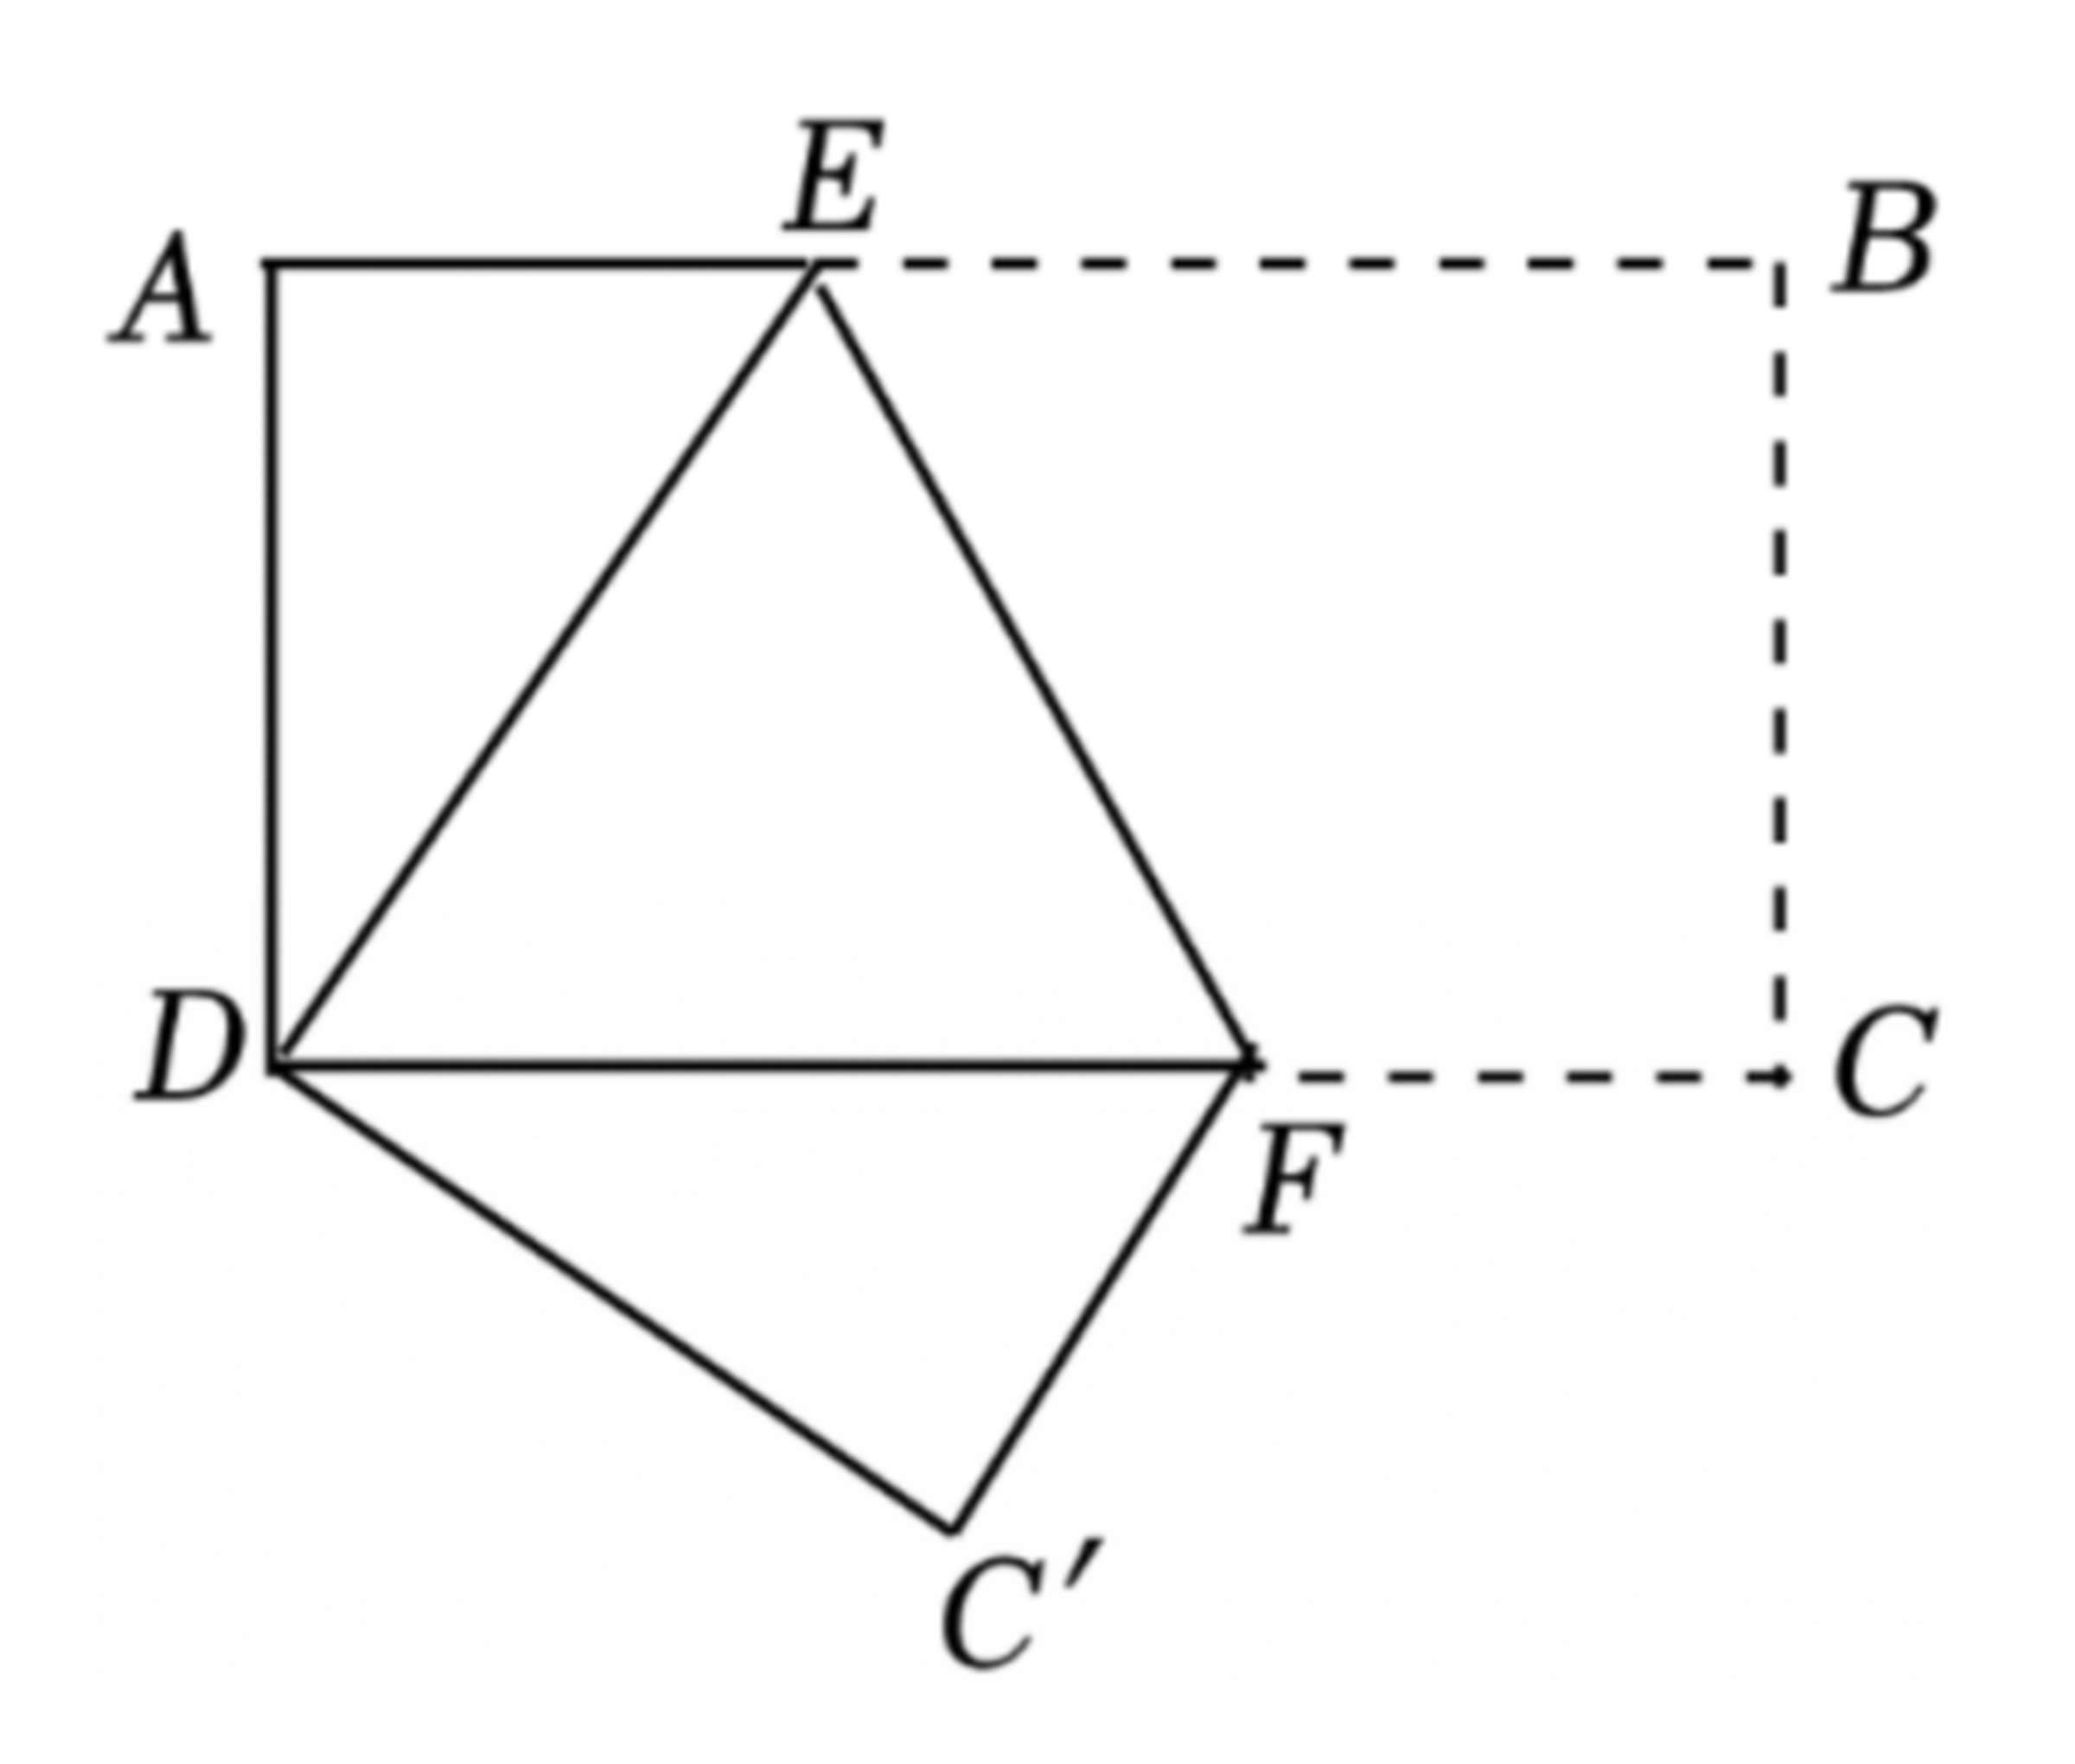
\includegraphics[width=0.40\textwidth]{figures/gao149_q11.png}
\end{center}

\ifanswer
\solbegin
\step{因为矩形 $ABCD(AB>AD)$ 的周长为 12，}
\step{在 $AB$ 和 $CD$ 边上分别取点 $E$ 和 $F$，将四边形 $BCFE$ 沿 $EF$ 折叠，}
\step{使点 $B$ 与点 $D$ 重合，此时点 $C$ 的对应点为 $C'$，}
\step{所以设 $AD=a$，$AB=b$，则 $2(a+b)=12$，}
\step{所以 $a+b=6$，且 $AB>AD$，所以 $b>a>0$，}
\step{设 $DF=x$，则 $C'F=b-x$，在 $Rt\triangle DC'F$ 中，$DC'=BC=a$，}% 几何三角形符号原卷印扁等边细线三角 $\triangle$，照录（放大 02 页确认）；$Rt$ 照录
\step{所以 $a^2+(b-x)^2=x^2$，解得 $x=\dfrac{a^2+b^2}{2b}$，}
\step{因此 $\triangle C'DF$ 的面积 $S=\dfrac{1}{2}\cdot DC'\cdot C'F=\dfrac{1}{2}\cdot a\cdot(b-x)$，}
\step{又 $b-x=b-\dfrac{(6-b)^2+b^2}{2b}=\dfrac{6(b-3)}{b}$，}
\step{所以 $S=\dfrac{1}{2}\cdot a\cdot\dfrac{6(b-3)}{b}=\dfrac{1}{2}\cdot(6-b)\cdot\dfrac{6(b-3)}{b}=\dfrac{3(6-b)(b-3)}{b}$}
\step{$=3\cdot\left(-b-\dfrac{18}{b}+9\right)$，又 $b+\dfrac{18}{b}\geqslant2\sqrt{b\cdot\dfrac{18}{b}}=6\sqrt{2}$，}
\step{当且仅当 $b=\dfrac{18}{b}$ 即 $b=3\sqrt{2}$ 时取等号，此时满足 $b>a$，}
\step{所以 $S\leqslant3\cdot(-6\sqrt{2}+9)=27-18\sqrt{2}$，故 $\triangle C'DF$ 面积的最大值为 $27-18\sqrt{2}$.}
\solend
\fi

% === Q12 === 解析内 3 幅三次函数曲线坐标图（仅答案版出）；解析 15 行（8 行 03 页＋7 行 04 页）
\item 已知 $m>0$，若存在 $t\in\R$，使得对任意 $x\in[0,m]$，不等式 $[(x-1)^2-t](x-t)\leqslant0$ 恒成立，则 $m$ 的最大值是\blankline[4.4em].

\ifanswer
\solbegin
\step{当 $t\leqslant0$ 时，$(x-1)^2-t\geqslant0$ 恒成立，}
\step{不等式 $[(x-1)^2-t](x-t)\leqslant0$ 的解集为 $x\leqslant t$，与 $x\in[0,m]$ 矛盾；}
\step{当 $t>0$ 时，不等式 $[(x-1)^2-t](x-t)\leqslant0\Leftrightarrow(x-1-\sqrt t)(x-1+\sqrt t)(x-t)\leqslant0$，}
\step{若 $t<1-\sqrt t$，即 $t\in\left(0,\dfrac{3-\sqrt5}{2}\right)$，}
\begin{center}
% 情形一 $t<1-\sqrt t$ 曲线图取 03 页右侧，去粉色水印、去色、4× LANCZOS 放大；仅答案版出
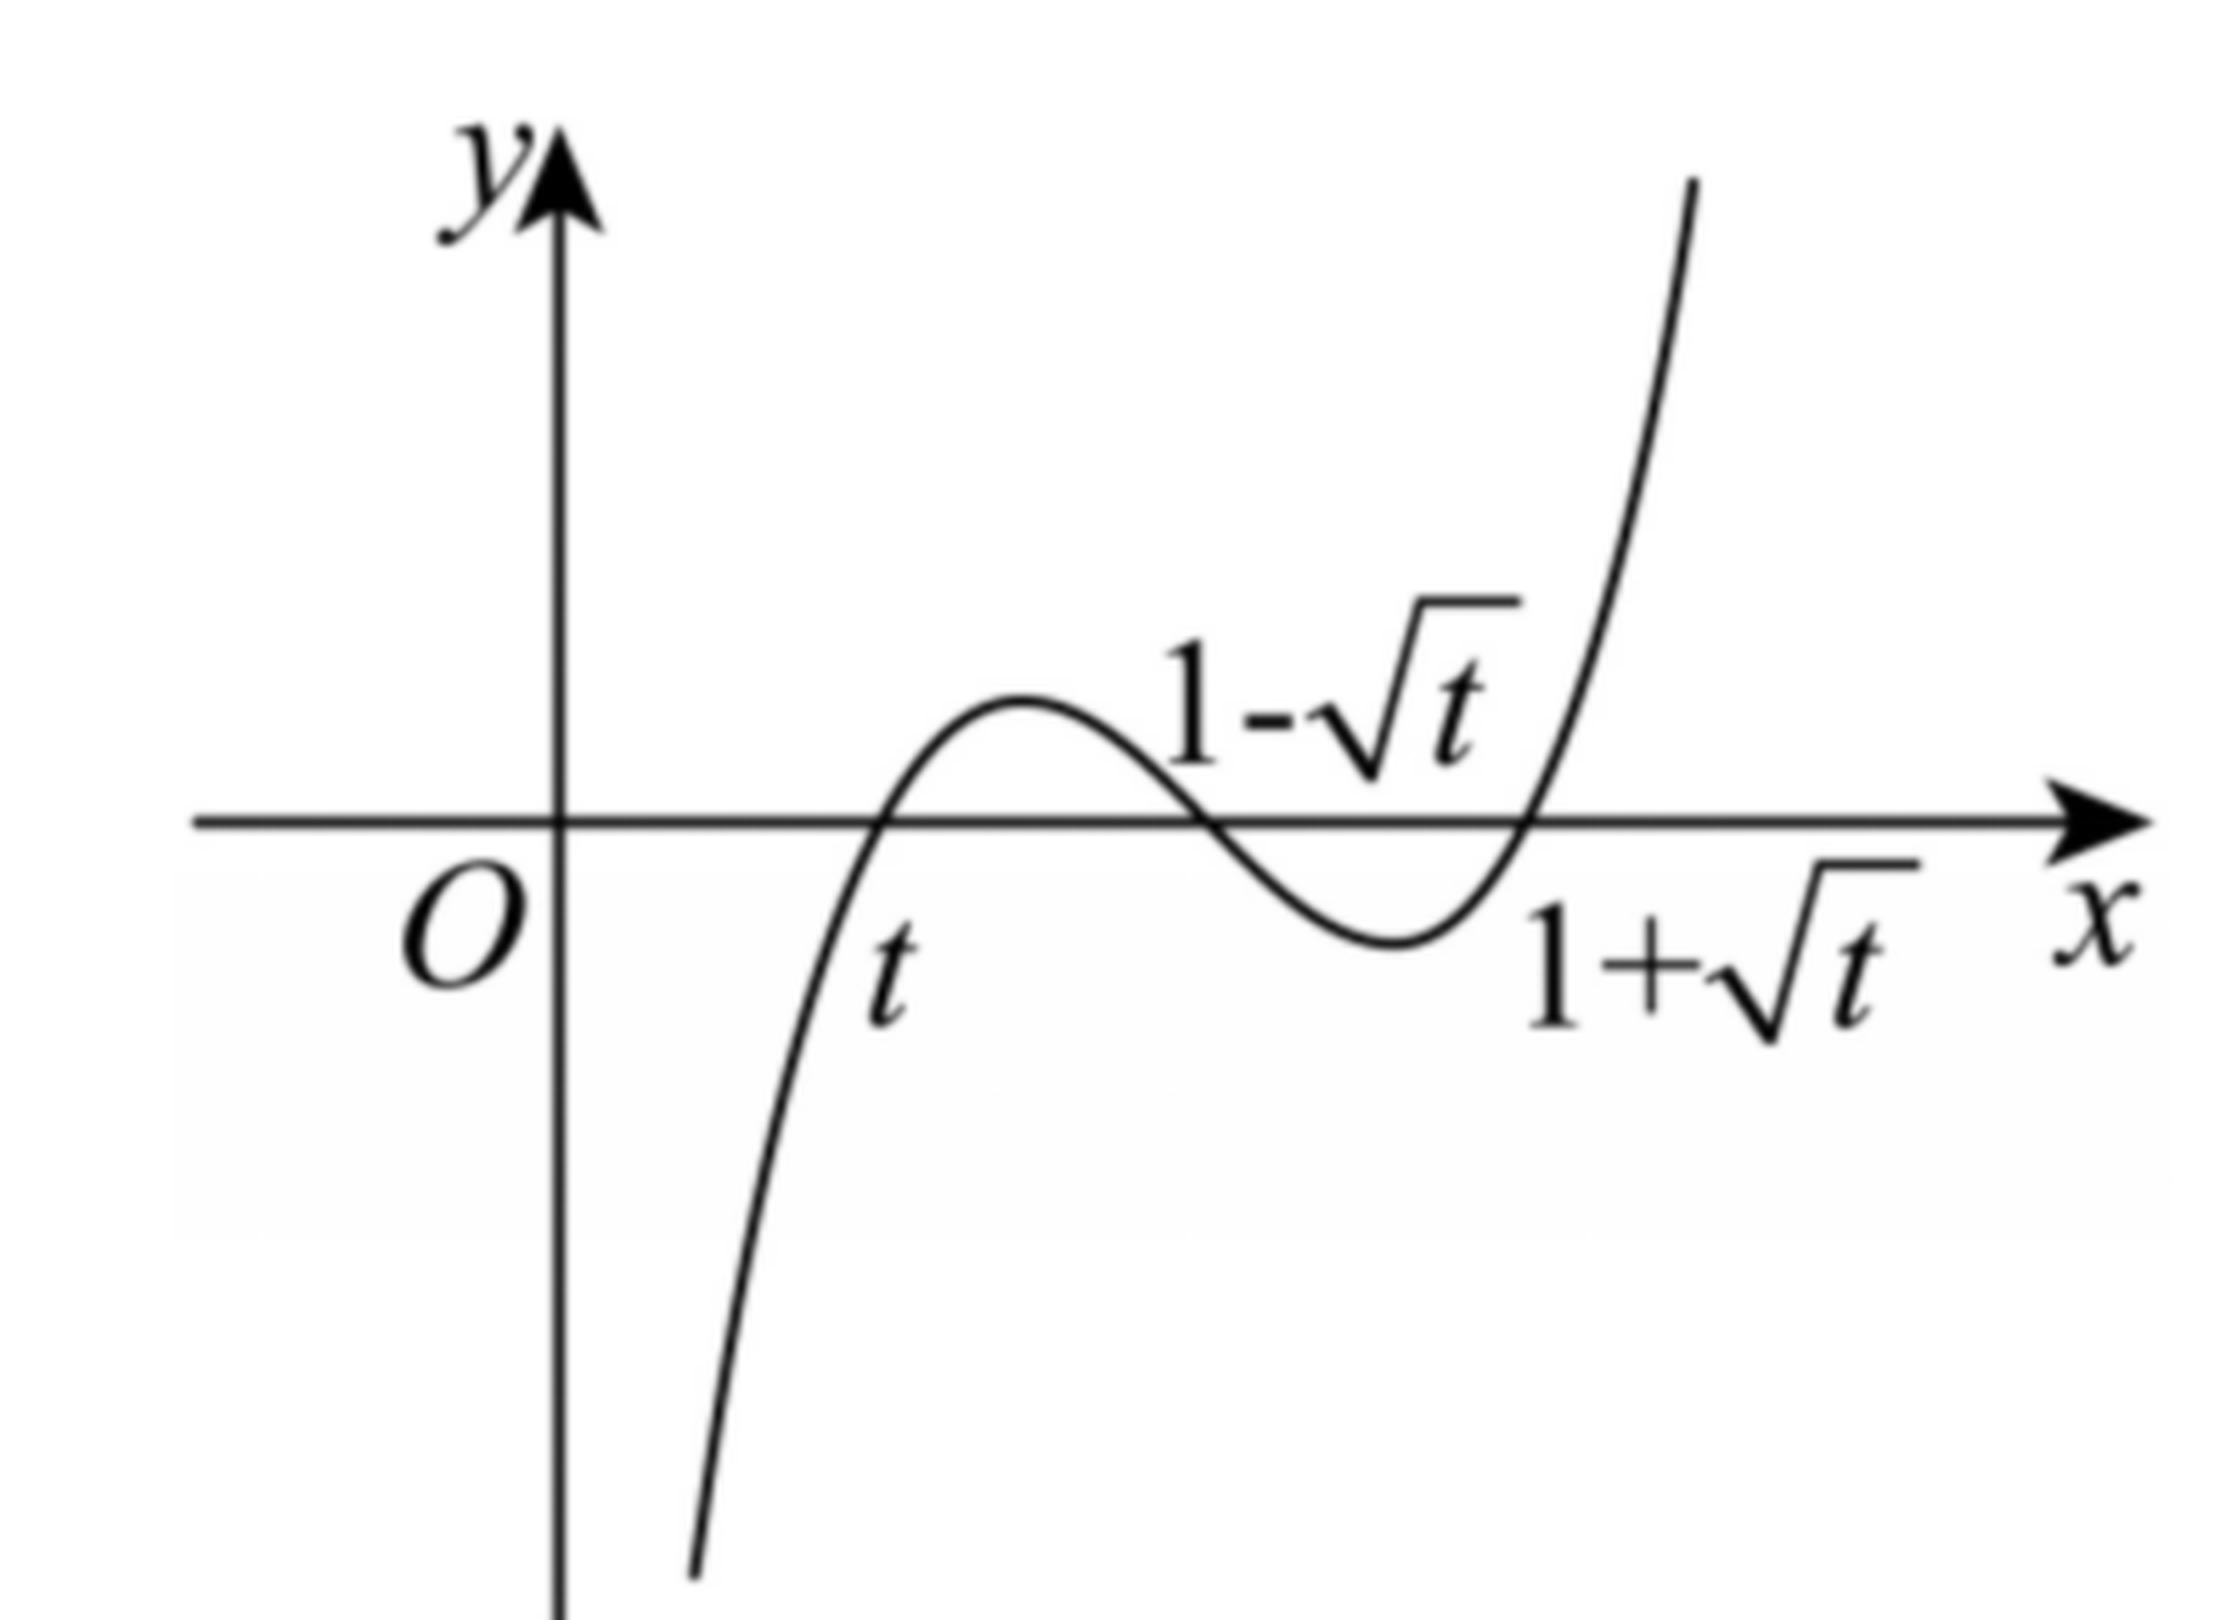
\includegraphics[width=0.40\textwidth]{figures/gao149_q12_a.png}
\end{center}
\step{则原不等式的解集为 $(-\infty,t]\cup[1-\sqrt t,1+\sqrt t]$，}
\step{当 $0<m\leqslant t$ 时，原不等式恒成立，因此}
\step{$m\in\left(0,\dfrac{3-\sqrt5}{2}\right)$；}
\step{若 $t=1-\sqrt t$，即 $t=\dfrac{3-\sqrt5}{2}$，则原不等式的解集为 $(-\infty,1+\sqrt t]$，}
\begin{center}
% 情形二 $t=1-\sqrt t$ 曲线图取 03 页右侧，去粉色水印、去色、4× LANCZOS 放大；仅答案版出
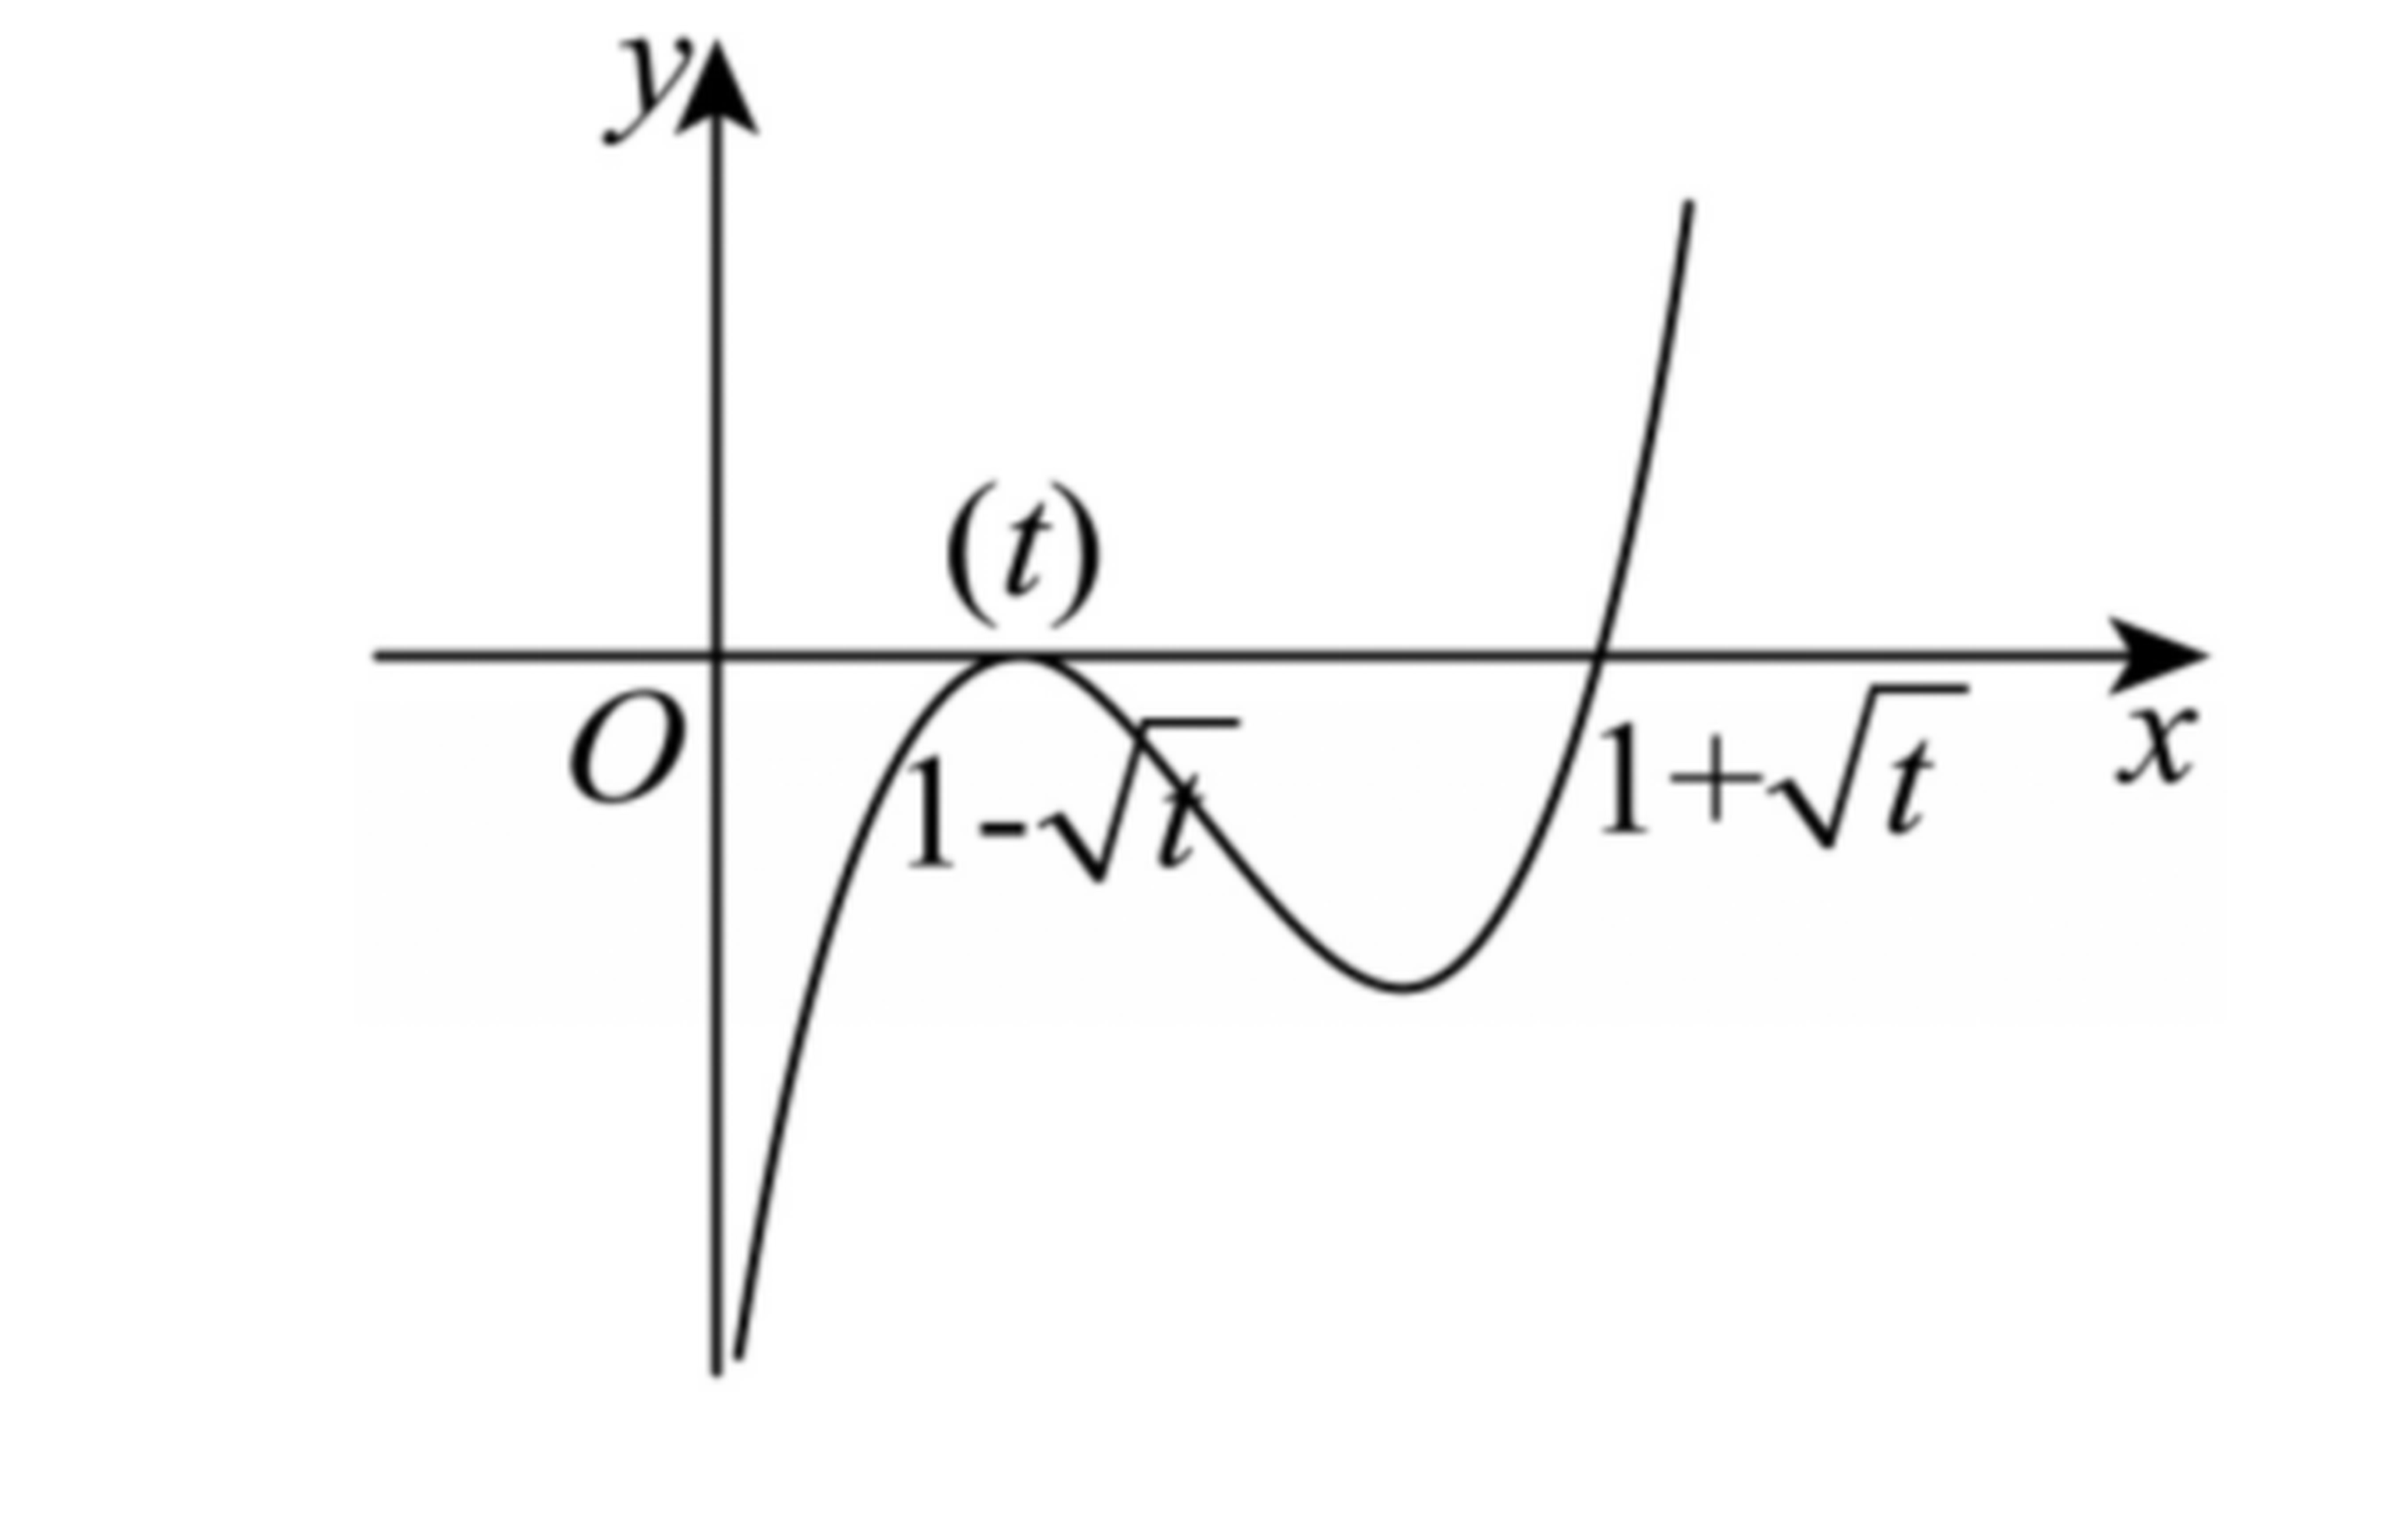
\includegraphics[width=0.40\textwidth]{figures/gao149_q12_b.png}
\end{center}
\step{当 $0<m\leqslant1+\sqrt t$ 时，原不等式恒成立，因此 $m\in\left(0,\dfrac{\sqrt5+1}{2}\right]$；}
\step{若 $1+\sqrt t>t>1-\sqrt t$，即 $t\in\left(\dfrac{3-\sqrt5}{2},\dfrac{3+\sqrt5}{2}\right)$，}
\begin{center}
% 情形三 $1+\sqrt t>t>1-\sqrt t$ 曲线图取 04 页右侧，去粉色水印、去色、4× LANCZOS 放大；仅答案版出
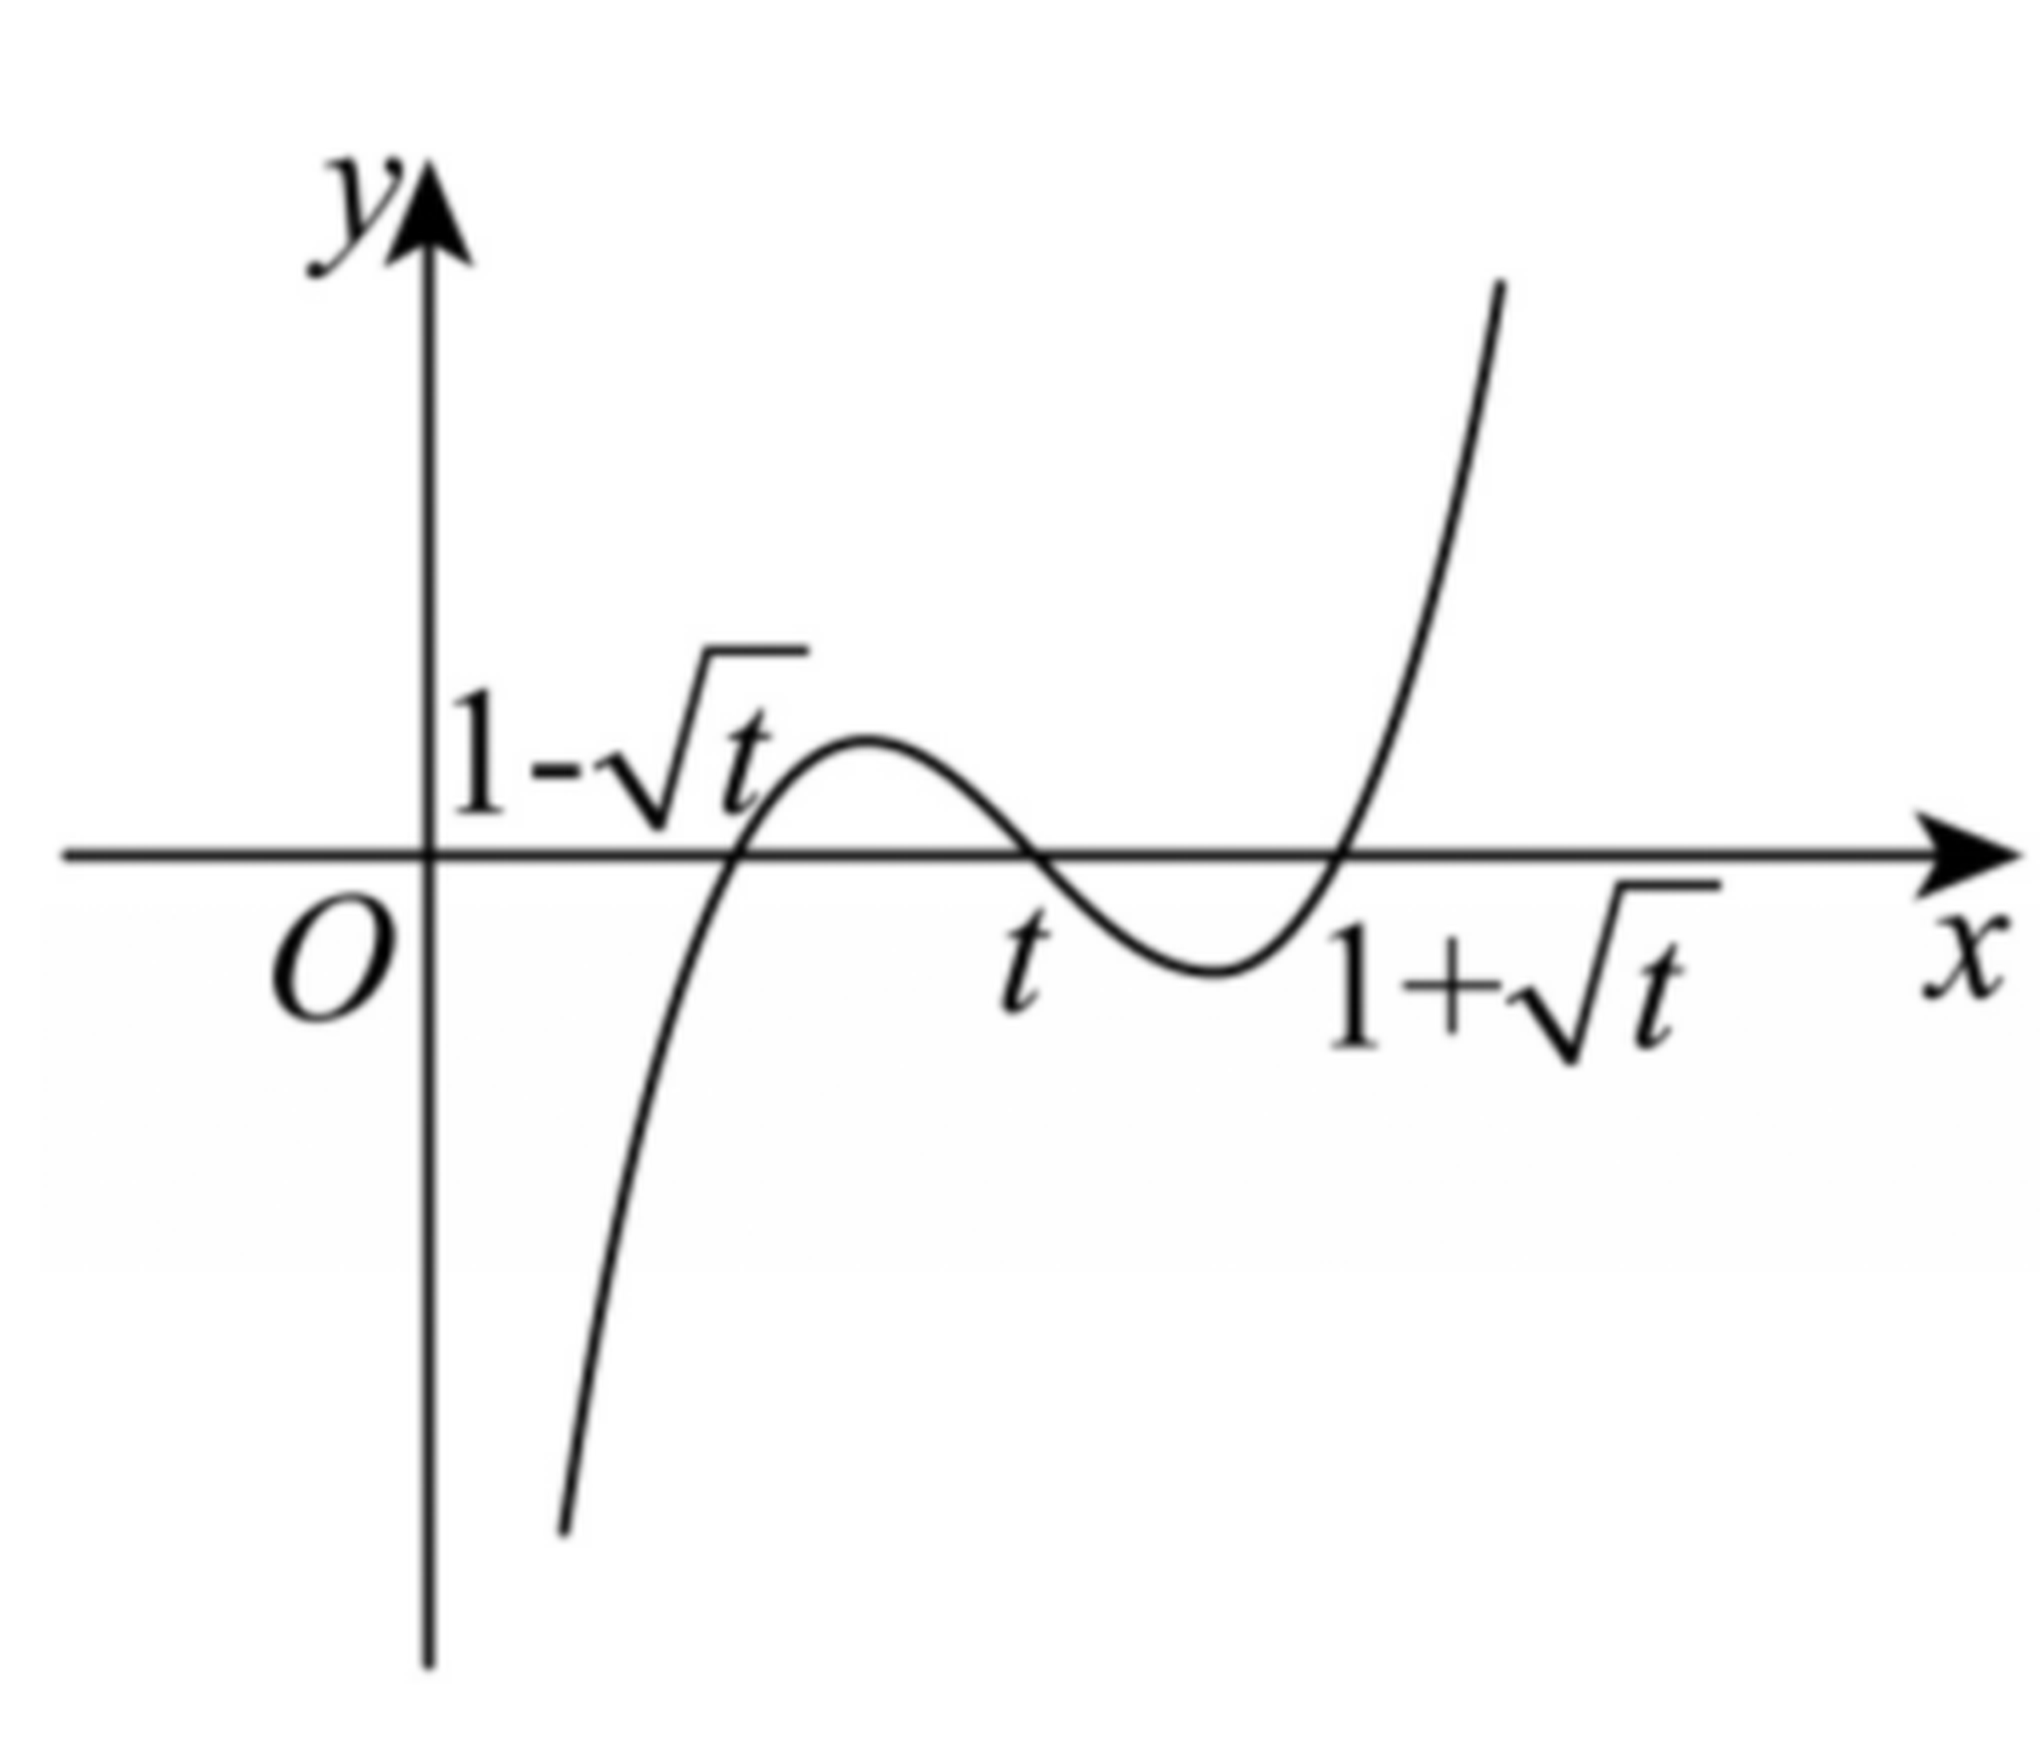
\includegraphics[width=0.40\textwidth]{figures/gao149_q12_c.png}
\end{center}
\step{则原不等式的解集为 $(-\infty,1-\sqrt t]\cup[t,1+\sqrt t]$，}
\step{当 $\begin{cases}1-\sqrt t>0\\1-\sqrt t\geqslant m\end{cases}$ 时，原不等式恒成立，此时 $t\in\left(\dfrac{3-\sqrt5}{2},1\right)$，$m\in\left(0,\dfrac{3-\sqrt5}{2}\right)$；}
\step{若 $t\geqslant1+\sqrt t$，即 $t\geqslant\dfrac{3+\sqrt5}{2}$，则取 $x=0$，$(t-1)t>0$，}
\step{原不等式不恒成立，不符合题意，}
\step{因此实数 $m$ 的取值范围是 $\left(0,\dfrac{\sqrt5+1}{2}\right]$，$m$ 的最大值是 $\dfrac{\sqrt5+1}{2}$.}
\solend
\fi

\end{enumerate}

\bigsec{二、选择题}

\begin{enumerate}
\setcounter{enumi}{12}

% === Q13 ===：答案"C"直接印在题干括号内、无【答案】/【解析】段，按 高一84 Q13／高一148 Q13 成例括号留空、另提 \ans{$C$}；四选项两行两列照原卷分行
\item 设 $ab>0$，则 $a>b$ 是 $\dfrac{1}{a}<\dfrac{1}{b}$ 的\mbox{（\quad）}

\keepwithprev
A. 充分不必要条件\qquad\qquad B. 必要不充分条件

C. 充要条件\qquad\qquad D. 既不充分又不必要条件

\ifanswer
\ans{$C$}
\fi

% === Q14 ===：$A\subset B$ 单线照录；四选项补集照原卷上划线 \overline{A}／\overline{B}；解析 1 行（由韦恩图得 B 对）
\item 已知集合 $A$、$B$ 非空，且 $A\subset B$，则下列式子中一定是空集的为\mbox{（\quad）}

\keepwithprev
A. $\overline{A}\cap B$\qquad B. $A\cap\overline{B}$\qquad C. $\overline{A}\cap\overline{B}$\qquad D. $\overline{A}\cup\overline{B}$

\ifanswer
\solbegin
\step{由韦恩图得 $B$ 对. 故选 $B$.}
\solend
\fi

% === Q15 ===："天文数字"弯引号照录；解析 2 行（首行在 04 页末、末行续 05 页顶）
\item 历史上数学计算方面的三大发明是阿拉伯数字、十进制和对数，其中对数的发明，大大缩短了计算时间，为人类研究科学和了解自然起了重大作用，对数运算对估算“天文数字”具有独特的优势. $2.5^{1000}$ 的估算值约为\mbox{（\quad）}

\keepwithprev
A. $10^{365}$\qquad B. $10^{379}$\qquad C. $10^{389}$\qquad D. $10^{398}$

\ifanswer
\solbegin
\step{$\lg 2.5^{1000}=1000\lg 2.5=1000(1-2\lg 2)\approx1000\times(1-0.602)=398$，}
\step{所以 $2.5^{1000}\approx10^{398}$. 故选 $D$.}
\solend
\fi

% === Q16 ===："完美集"新定义、圈数字①②文本模式；题干"若对任意 $x$，$y\in A$"用全角逗号、解析用顿号"$x$、$y\in A$"，两处照录不统一；解析 9 行
\item 设全集 $U=\R$，集合 $A$ 是一个非空数集，若对任意 $x$，$y\in A$，都有 $x+y\in A$、$xy\in A$，则称集合 $A$ 为一个“完美集”，给出以下命题：

①若 $A_1$、$A_2$ 都是“完美集”，且 $A_1\cap A_2\ne\varnothing$，则 $A_1\cap A_2$ 也是“完美集”；

②若 $A_1$、$A_2$ 都是“完美集”，则 $A_1\cup A_2$ 也是“完美集”.

下列说法正确的是\mbox{（\quad）}

\keepwithprev
A. ①②都是真命题\qquad\qquad B. ①是真命题，②是假命题

C. ①是假命题，②是真命题\qquad\qquad D. ①②都是假命题

\ifanswer
\solbegin
\step{由题意，全集 $U=\R$，集合 $A$ 是一个非空数集，}
\step{若对任意 $x$、$y\in A$，都有 $x+y\in A$、$xy\in A$，则称集合 $A$ 为一个“完美集”，}
\step{对于①，取 $x$、$y\in A_1\cap A_2$，则 $x\in A_1$，$x\in A_2$，$y\in A_1$，$y\in A_2$，}
\step{又 $A_1$、$A_2$ 是“完美集”，所以 $x+y\in A_1$，$xy\in A_1$，$x+y\in A_2$，$xy\in A_2$，}
\step{所以 $x+y\in A_1\cap A_2$，$xy\in A_1\cap A_2$，所以 $A_1\cap A_2$ 是“完美集”，故①正确；}
\step{对于②，取“完美集” $A_1=\{x\mid x=2k,k\in\Z\}$，$A_2=\{x\mid x=3k,k\in\Z\}$，}
\step{则 $2\in A_1$，$3\in A_2$，但 $2+3\notin A_1\cup A_2$，}
\step{即此时 $A_1\cup A_2$ 不是“完美集”，故②错误.}
\step{故选 $B$.}
\solend
\fi
\end{enumerate}

\bigsec{三、解答题}

\begin{enumerate}
\setcounter{enumi}{16}

% === Q17 ===："图像"（有亻）照录（Q17 题干与解析共 2 处）；绝对值 \lvert…\rvert；解析 7 行
\item 已知 $m\in\R$，$f(x)=(m^2-m-5)x^m$. 若 $y=f(x)$ 是幂函数，且其图像不经过原点.

(1) 求实数 $m$ 的值；

(2) 若 $f(a)=f(b)$ 且 $a\ne b$，求 $\lvert a+2\rvert+\lvert b-1\rvert$ 的最小值，并指出取到最小值时 $a$ 的取值范围.

\ifanswer
\solbegin
\step{(1) $f(x)=(m^2-m-5)x^m$ 是幂函数，得 $m^2-m-5=1$，即 $m^2-m-6=0$，}
\step{解得 $m=-2$ 或 $m=3$，又函数图像不经过原点，所以 $m=-2$($3$ 舍)；}
\step{(2) 由 (1) 得 $f(x)=x^{-2}=\dfrac{1}{x^2}$ 为偶函数，}
\step{$x<0$ 时，函数 $f(x)$ 严格增，$x>0$ 时，函数 $f(x)$ 严格减，}
\step{又 $f(a)=f(b)$ 且 $a\ne b$，所以 $a=-b$，且 $a\ne0$，$b\ne0$，}
\step{则 $\lvert a+2\rvert+\lvert b-1\rvert=\lvert a+2\rvert+\lvert-a-1\rvert=\lvert a+2\rvert+\lvert a+1\rvert$，}
\step{则 $\lvert a+2\rvert+\lvert b-1\rvert$ 的最小值为 $1$，取到最小值时 $a$ 的取值范围是 $[-2,-1]$.}
\solend
\fi

% === Q18 ===：判别式两形混用——(1) cases 块印高 \Delta、(2) 独立行印扁 \triangle，逐处照录不统一；解析 8 行
\item 已知命题 $p$：方程 $x^2+4x+m-1=0$ 有两个不等的负根；命题 $q$：方程 $4x^2+4x+m-2=0$ 无实根.

(1) 若 $p$ 为真命题，求 $m$ 的取值范围；

(2) 若 $p$、$q$ 两命题一真一假，求 $m$ 的取值范围.

\ifanswer
\solbegin
\step{(1) 若 $p$ 为真命题，即方程 $x^2+4x+m-1=0$ 有两个不等的负根；}
\step{必有 $\begin{cases}\Delta=16-4(m-1)>0\\m-1>0\end{cases}$，解得 $1<m<5$，即 $m$ 的取值范围为 $(1,5)$；}
\step{(2) 命题 $q$：方程 $4x^2+4x+m-2=0$ 无实根，}
\step{则有 $\triangle=16-16(m-2)<0$，解得 $m>3$，}
\step{若 $p$ 和 $q$ 有且只有一个为真命题，}
\step{若 $p$ 真 $q$ 假，必有 $\begin{cases}1<m<5\\m\leqslant3\end{cases}$，则有 $1<m\leqslant3$，}
\step{若 $p$ 假 $q$ 真，必有 $\begin{cases}m\leqslant1\text{ 或 }m\geqslant5\\m>3\end{cases}$，则有 $m\geqslant5$，}
\step{综上，$1<m\leqslant3$ 或 $m\geqslant5$.}
\solend
\fi

% === Q19 ===：$A\subseteq B$ 带下划线照录；解析 7 行（(2) 两组 cases 并排）
\item 已知 $m\in\R$，集合 $A=\left\{x\mid y=\sqrt{3-x}-\dfrac{1}{\sqrt{x-1}}\right\}$，集合 $B=\{x\mid 2m\leqslant x\leqslant1-m\}$.

(1) 若 $A\cup B=B$，求实数 $m$ 的取值范围；

(2) 若 $A\cap B=\varnothing$，求实数 $m$ 的取值范围.

\ifanswer
\solbegin
\step{(1) 函数 $y=\sqrt{3-x}-\dfrac{1}{\sqrt{x-1}}$，则 $\begin{cases}3-x\geqslant0\\x-1>0\end{cases}$，解得 $1<x\leqslant3$，}
\step{所以 $A=\{x\mid1<x\leqslant3\}$，}
\step{因为 $A\cup B=B$，所以 $A\subseteq B$，则 $\begin{cases}2m\leqslant1\\1-m\geqslant3\end{cases}$，解得 $m\leqslant-2$，}
\step{综上，实数 $m$ 的取值范围为 $(-\infty,-2]$；}
\step{(2) 当 $B=\varnothing$ 时，则 $2m>1-m$，解得 $m>\dfrac{1}{3}$，}
\step{当 $B\ne\varnothing$ 时，则 $\begin{cases}2m\leqslant1-m\\2m>3\end{cases}$ 或 $\begin{cases}2m\leqslant1-m\\1-m\leqslant1\end{cases}$，解得 $m\in\varnothing$ 或 $0\leqslant m\leqslant\dfrac{1}{3}$，}
\step{综上，实数 $m$ 的取值范围为 $[0,+\infty)$.}
\solend
\fi

% === Q20 ===：n 阶基本不等式推广；(3) 解析含 \overbrace{…}^{k} 上括号；(2) 解析"x=x=x=3(1-x)"三连等系原卷笔误、照录加注（见 ⑤）；解析 14 行
\item 教材中的基本不等式可以推广到 $n$ 阶：$n$ 个正数的算术平均数不小于它们的几何平均数，即对于任意的正数 $a_1$、$a_2$、$\cdots$、$a_n$，有 $\dfrac{a_1+a_2+\cdots+a_n}{n}\geqslant\sqrt[n]{a_1\cdot a_2\cdots a_n}$（$n\in\N$ 且 $n\geqslant2$），且等号当且仅当 $a_1=a_2=\cdots=a_n$ 时成立. 利用此结论解决下列问题：

(1) 若 $x$、$y$、$z>0$，求 $\dfrac{y}{x}+\dfrac{2z}{y}+\dfrac{4x}{z}$ 的最小值；

(2) 已知 $0<x<1$，求 $x^3(1-x)$ 的最大值，并求取得最大值时的 $x$ 的值；

(3) 对任意的正整数 $k$，判断 $\left(1+\dfrac{1}{k}\right)^k$ 与 $\left(1+\dfrac{1}{k+1}\right)^{k+1}$ 的大小关系，并证明.

\ifanswer
\solbegin
\step{(1) 因为 $x$、$y$、$z>0$，有 $\dfrac{y}{x}>0$，$\dfrac{2z}{y}>0$，$\dfrac{4x}{z}>0$}
\step{所以 $\dfrac{y}{x}+\dfrac{2z}{y}+\dfrac{4x}{z}\geqslant3\sqrt[3]{\dfrac{y}{x}\cdot\dfrac{2z}{y}\cdot\dfrac{4x}{z}}=3\sqrt[3]{8}=6$，}
\step{当且仅当 $\dfrac{y}{x}=\dfrac{2z}{y}=\dfrac{4x}{z}$ 时取等号，故 $\dfrac{y}{x}+\dfrac{2z}{y}+\dfrac{4x}{z}$ 的最小值为 $6$.}
\step{(2) 因为 $0<x<1$，所以 $1-x>0$，}
\step{$x^3(1-x)=\dfrac{1}{3}[x\cdot x\cdot x\cdot3(1-x)]\leqslant\dfrac{1}{3}\left[\dfrac{x+x+x+3(1-x)}{4}\right]^4=\dfrac{1}{3}\times\left(\dfrac{3}{4}\right)^4$}
\step{$=\dfrac{27}{256}$，当且仅当 $x=x=x=3(1-x)$，即 $x=3(1-x)$，$x=\dfrac{3}{4}$ 取等号，}% 原卷"x=x=x=3(1-x)"三连等，疑为四因子相等之误排，放大 08 页确认，照录未改（见 ⑤）
\step{所以 $0<x<1$ 时，$x^3(1-x)$ 的最大值是 $\dfrac{27}{256}$，取最大值时 $x=\dfrac{3}{4}$.}
\step{(3) 对任意 $k\in\N^*$，$\left(1+\dfrac{1}{k}\right)^k<\left(1+\dfrac{1}{k+1}\right)^{k+1}$.}
\step{证明：$\left(1+\dfrac{1}{k}\right)^k=\overbrace{\left(1+\dfrac{1}{k}\right)\cdot\left(1+\dfrac{1}{k}\right)\cdots\left(1+\dfrac{1}{k}\right)}^{k}\times1$}
\step{$\leqslant\left(\dfrac{\overbrace{\left(1+\dfrac{1}{k}\right)+\left(1+\dfrac{1}{k}\right)+\cdots+\left(1+\dfrac{1}{k}\right)}^{k}+1}{k+1}\right)^{k+1}$}
\step{$=\left(\dfrac{\overbrace{(1+1+\cdots+1)}^{k}+\overbrace{\left(\dfrac{1}{k}+\dfrac{1}{k}+\cdots+\dfrac{1}{k}\right)}^{k}+1}{k+1}\right)^{k+1}=\left(\dfrac{k+1+1}{k+1}\right)^{k+1}=\left(1+\dfrac{1}{k+1}\right)^{k+1}$，}
\step{当且仅当 $1+\dfrac{1}{k}=1$ 时取等号，}
\step{但是任意 $k\in\N^*$ 时 $1+\dfrac{1}{k}>1$，所以等号不成立，}
\step{故任意 $k\in\N^*$ 时，$\left(1+\dfrac{1}{k}\right)^k<\left(1+\dfrac{1}{k+1}\right)^{k+1}$.}
\solend
\fi

% === Q21 ===："减 k 集"新定义（引号内 k／数字两侧空格照录）；解析 26 行（续 10 页），含 ⑤ 三处原卷笔误照录
\item 定义：对于给定的整数 $k$，若非空集合 $A$ 满足如下 3 个条件：

① $A$ 是正整数集的子集；② $A\ne\{1\}$；

③对任意正整数 $x,y$，若 $x+y\in A$，则 $xy-k\in A$；则称集合 $A$ 为“减 $k$ 集”.

(1) 判断集合 $A=\{1,2\}$ 是否为“减 $0$ 集”？是否为“减 $1$ 集”？（无需说明理由）

(2) 证明：不存在“减 $2$ 集”；

(3) 是否存在“减 $1$ 集”？如果存在，求出所有“减 $1$ 集”；如果不存在，说明理由.

\ifanswer
\solbegin
\step{(1) 因为 $P\subseteq\N^*$，$P\ne\{1\}$，$1+1=2\in P$，$1\times1-0\in P$，}
\step{所以集合 $P=\{1,2\}$ 是“减 $0$ 集”；}
\step{因为 $P\subseteq\N^*$，$P\ne\{1\}$，$1+1=2\in P$，$1\times1-1\notin P$，}
\step{所以集合 $P=\{1,2\}$ 是“减 $1$ 集”；}% 按条件③应为"不是"，原卷径印"是"，放大 09 页确认，照录未改（见 ⑤）
\step{(2) 假设存在集合 $A$ 是“减 $2$ 集”，若 $x+y\in A$，则 $xy-2\in A$，}
\step{①当 $x+y=xy-2$ 时，有 $(x-1)(y-1)=3$，}
\step{则 $x$、$y$ 一个为 $2$，一个为 $4$，所以集合 $A$ 有元素 $6$，}
\step{但 $3+3\in A$，$3\times3-2\notin A$，与 $A$ 是“减 $2$ 集”矛盾；}
\step{②当 $x+y\ne xy-2$ 时，则 $x+y=xy-1$ 或 $x+y=xy-m$($m>2$)，}
\step{若 $x+y=xy-1$，$m=1$ 时，$M$ 为除 $1$ 以外的最小元素，}% 原卷"m=1"上文未显式定义，疑笔误，放大 09 页确认，照录未改（见 ⑤）
\step{则 $x=M-1$，$y=1$ 时，$xy-2=M-3$ 小于 $M$，}
\step{要符合题意，必须 $M=4$，}
\step{此时取 $x-2$，$y=2$，$xy-2=2$ 不属于 $A$，故不符合题意，}% 原卷"取 x−2"疑为"取 x=2"误排，放大 09 页确认，照录未改（见 ⑤）
\step{当 $m>2$ 时，$(x-1)(y-1)=m+1$，同样得出矛盾，}
\step{综上，不存在 $A$ 是“减 $2$ 集”.}
\step{(3) 存在“减 $1$ 集” $A$，则 $A\ne\{1\}$，}
\step{①假设 $1\in A$，则 $A$ 中除了元素 $1$ 以外，必然还含有其它元素，}
\step{假设 $2\in A$，$1+1\in A$，而 $1\times1-1\notin A$，所以 $2\notin A$，}
\step{假设 $3\in A$，$1+2\in A$，而 $1\times2-1\in A$，所以 $3\in A$，}
\step{所以 $A=\{1,3\}$，}
\step{假设 $4\in A$，$1+3\in A$，而 $1\times3-1\notin A$，所以 $4\notin A$，}
\step{假设 $5\in A$，$1+4\in A$，$1\times4-1\in A$，$2+3=5$，$2\times3-1\in A$，所以 $5\in A$，}
\step{所以 $A=\{1,3,5\}$，}
\step{以此类推，得 $A=\{1,3,5,\cdots,2n-1,\cdots\}$，($n\in\N^*$)，}
\step{所以所有的“减 $1$ 集”有 $\{1,3\}$，$\{1,3,5\}$，$\{1,3,5,7\}$，$\cdots$，$\{1,3,5,\cdots,2n-1,\cdots\}$，}
\step{$(n\in\N^*)$.}
\solend
\fi
\end{enumerate}

\end{document}
"
%
% ① 原始材料：微信公众号"魔都数学加油站"文章，连载"27学年高一149"，原文标题
% "27学年高一149——2026-2027年上海市青浦高级中学上外云间高一上期中"；
% 原文链接：https://mp.weixin.qq.com/s/T7_nyoR1k0o_5og7FkDsyw 。
% 正文为 10 张 PNG 页（01/02/03/04/10 为 2560×3620，05/06/07/08/09 为 4762×6735，
% 同一篇各页分辨率混排，逐页按各自分辨率裁图核对，别按预览比例换算裁框）。
% 体例：混合体例讲评版——19 题中 Q6 只印【答案】、无【解析】；Q13 的答案"C"
%   直接印在题干括号内、无【答案】/【解析】段；其余 17 题印【解析】（逐题核实，见 ② ②）。
% 题目、答案、解析均据原图转录；卷面粉红色水印"魔都数学加油站"及公众号页脚未录入。
% 全卷插图清单（逐页通读 10 页确认）：1 幅题目配图 + 3 幅【解析】内配图：
%   · Q11 矩形 ABCD 折叠几何图（02 页右侧：A/B/C/D/E/F/C' 与虚线 EB、BC、FC），
%     题干"如图"处，题目配图、三版都出，裁 figures/gao149_q11.png；
%   · Q12【解析】内 3 幅三次函数曲线坐标图（03 页右侧两幅 + 04 页右侧一幅：
%     x/y 轴、O、t、1-\sqrt t、1+\sqrt t 等标注，分别对应 t<1-\sqrt t、
%     t=1-\sqrt t、1+\sqrt t>t>1-\sqrt t 三种情形），解析配图、仅答案版出，
%     分别裁 figures/gao149_q12_a.png／_b.png／_c.png，放 \ifanswer 内 \step 之间
%     （高一73 第 16 题成例）；
%   其余各页逐页确认无其它题目配图、无表格；Q14 解析"由韦恩图得 B 对"仅文字推导、
%   原卷并未印韦恩图；Q9／Q18／Q19 的 cases 块与 Q20(3) 的 \overbrace 为数学块（非图）；
%   10 页下半仅水印、无正文。4 图均取自原卷截图，去粉色水印、去色、4× LANCZOS 放大。
%
% 卷首标题：原卷印作"2026-2027 年青浦高级中学上外云间高一上期中"，年份区间按全稿
% 惯例排 en dash；原卷卷面未印副标题，本稿按同期中卷（高一140／141／143／144／145／
% 146／147／148）知识模块口径补出"集合与常用逻辑用语、不等式、函数"。
%
% 题号体例（逐页核实定稿）：本卷共 19 题——一、填空题 3—12（10 题）、
% 二、选择题 13—16（4 题）、三、解答题 17—21（5 题）。
% 三节分别 \setcounter{enumi}{2}／{12}／{16}。原卷从第 3 题起、无第 1、2 题，
% 本稿保留原题号；全卷无附加题节（Q21 解析末行"（n\in N^*）."为全卷收尾）。
%
% ② 与原卷的排版差异：
%   ① 原文从第 3 题起，本稿保留原题号；共 19 题三节；
%   ② 混合体例逐题核实：Q6（反证法"假设的内容"）只印【答案】、无【解析】，
%      按 高一140 第 5 题／高一145 Q3 成例提 \ans{}、不补造解析；Q13 答案"C"直接
%      印在题干括号内、全卷无该题【答案】/【解析】段，按 高一84 Q13／高一148 Q13
%      成例括号 \mbox{（\quad）} 留空、另提 \ans{$C$}；其余 17 题印【解析】、
%      用 \solbegin…\solend，选择题答案在解析末句"故选 X"（Q14 选 B、Q15 选 D、
%      Q16 选 B，逐个放大 04/05 页核实）、题干括号留空、不另提 \ans{}；
%      答案版【答案】/【解析】标记数 = 19（2 个 \ans ＋ 17 个 \solbegin）
%      = 全卷题数；
%   ③ 原卷卷面未印副标题，本稿按知识模块口径补出；
%   ④ 原卷填空横线按全稿惯例排 \blankline[4.4em]；选择题括号排 \mbox{（\quad）}、
%      选项段前按惯例加 \keepwithprev；Q13／Q16 四选项为两行两列、Q14／Q15
%      选项为一行，照原卷分行；解答题不留作答区、不加 \anspace（原卷为讲评版）；
%   ⑤ 数集：Q6"a,b\in N"、Q8"x\in R"、Q9"a\in R"／"解集为 R"、Q12"t\in R"、
%      Q16"U=R"、Q17"m\in R"、Q19"m\in R"、Q20"n\in N" 原卷印斜体 R/N，
%      按全稿惯例统一改 \R／\N；Q20(3)、Q21 的 $N^*$ 排 \N^*；Q16 解析
%      "$k\in Z$" 排 \Z。绝对值排 \lvert…\rvert（Q17），集合描述竖线排 \mid
%      （Q19、Q16 解析）；不等号按全稿惯例排 \leqslant／\geqslant；
%      补集照原卷上划线排 \overline{A}／\overline{B}（Q14 四选项）；空集
%      \varnothing（Q16、Q19、Q21）；
%   ⑥ 子集符号逐处照录不统一：Q4 题干"{1,2}⊆A⊂{1,2,3,4,5,6}" 前者印带下划线
%      ⊆、照录 \subseteq，后者印单线 ⊂、照录 \subset；Q10"A⊆{-1,1/2,2,3}"、
%      Q19 解析"A⊆B"、Q21 解析"P⊆N*" 均印带下划线 ⊆、照录 \subseteq；
%      Q14"A⊂B" 印单线 ⊂、照录 \subset（逐处放大 01/02/04/07/09 页确认，见 ④）；
%   ⑦ 子题标号 (1)(2)(3) 半角括号照录；圈数字 ①②③ 在文本模式（Q16 两命题、
%      Q21 三个条件与解析的①②）按 common.sty 划入 CJK 字符类渲染；cases 块整体
%      算一个印刷行；\left…\right 不得拆到不同 $…$ 组；数学式内 CJK 用 \text{}
%      （Q18 解析 cases 块"\text{或}"）；Q11 解析"Rt\triangle DC'F" 的 Rt 照录；
%   ⑧ 题干／解析中的中文弯引号按原卷照录：Q6" 已知 a,b\in N，若 ab 能被 5 整除，
%      那么 a、b 中至少有一个能被 5 整除 "（开引号后紧跟"已知"、闭引号后空格接"时"）、
%      Q15"天文数字"、Q16"完美集"、Q21"减 k 集""减 0 集""减 1 集""减 2 集"
%      （引号内 k／数字两侧有空格），注释内一律 ASCII 引号；
%   ⑨ 半角逗号在数学组之间是全稿惯例、非笔误（Q8"$a>0,a\ne1,x\in\R$"、
%      Q21 题干"$x,y$" 等），逐处照录别改；Q16 题干"若对任意 $x$，$y\in A$"
%      用全角逗号而解析用顿号"$x$、$y\in A$"，两处不同均照录；行末西文句点
%      照录为 ASCII `.`；行中全角逗号／顿号照录；
%   ⑩ "图像／图象"逐处放大核：Q10 题干与解析共 6 处均印"图象"（象，无亻）；
%      Q17 题干"其图像不经过原点"与解析"又函数图像不经过原点" 2 处印"图像"
%      （像，有亻），逐处照录未统一改动（放大 02/05/06 页确认）；
%   ⑪ 判别式 Δ/△ 混用是照录项：Q9 解析 cases 块"Δ=4(a−2)²+16(a−2)<0"、
%      Q18(1) cases 块"Δ=16−4(m−1)>0" 两处印等腰偏高粗三角 \Delta；
%      Q18(2) 独立行"△=16−16(m−2)<0" 印扁等边细线三角 \triangle，
%      逐处放大判断、照录不统一（参照 高一142／144／145／146／148 头注④口径）；
%      另 Q11 题干"△C'DF 面积"与解析 3 处"△"（含"Rt△DC'F"）共 4 处几何
%      三角形符号亦印扁细线三角，照录 \triangle（非判别式，字形同类，见 ④）；
%   ⑫ 一条 \step = 原卷解析的一个印刷行，cases 块整体算一个印刷行；别把原卷折行
%      并起来、别把一行拆多条。Q11 十三行（7 行在 02 页＋6 行在 03 页）、
%      Q12 十五行（8 行在 03 页＋7 行在 04 页）、Q16 九行、Q21 二十六行
%      （续 10 页）均按印刷行逐条断，不丢行；
%   ⑬ 配图：Q11 题目配图（三版都出）放 \item 内题干之后 \begin{center}，
%      大图块加 \needvspace{8cm} 守卫把整块推走（守卫放 \item 之前，见
%      高一145 Q14/Q20 成例与切页审计 B 类坑）；Q12 三幅解析配图（仅答案版出）
%      放 \ifanswer 内 \solbegin…\solend 的 \step 之间；三版切页审计均"合计异常：无"；
%   ⑭ 跨页续印按题合并：Q3/4/5 在 01 页；Q6/7/8 题干与解析在 01 页；
%      Q9 题干在 01 页末、解析 4 行在 02 页顶；Q10 题干＋解析在 02 页；
%      Q11 题干＋图＋解析前 7 行在 02 页、解析后 6 行续 03 页顶；
%      Q12 题干＋解析首行在 03 页末、解析续 7 行在 03 页下半＋7 行在 04 页顶，
%      "二、选择题"标题在 04 页下半；Q13/14 题干＋选项＋Q14 解析在 04 页下半；
%      Q15 题干＋选项＋解析首行在 04 页末、末行"所以 2.5^1000≈10^398. 故选 D."
%      续 05 页顶；Q16 题干＋选项＋解析 9 行在 05 页、"三、解答题"标题＋
%      Q17 题干首句在 05 页末；Q17(2)＋解析 7 行、Q18 题干＋解析前 6 行在 06 页；
%      Q18 解析末 2 行续 07 页顶；Q19 题干＋解析 4 行在 07 页上半、
%      解析续 3 行在 07 页下半；Q20 题干(1) 在 07 页末、题干(2)(3)＋解析(1)(2)
%      在 08 页上半、(3) 解析含 \overbrace 的证明在 08 页下半、末行
%      "故任意 k∈N* 时…"续 09 页顶；Q21 题干＋解析(1)(2)(3) 前段在 09 页、
%      解析(3) 后半 9 行续 10 页上半（10 页下半仅水印、无正文）。
%      本稿按题连排，不丢行、不并折行；
%   ⑮ 原卷解析内无红色"法一／法二"之类小标题，故本卷无 \stepm；水印
%      "魔都数学加油站"红色不录入。
%
% ③ 行数复核：一条 \step／\stepm = 原卷解析的一个印刷行，cases 块作一个印刷行计。
%   逐题数（主会话逐页核对定稿）：Q3：1；Q4：2；Q5：2；Q6：0（只印【答案】、
%   提 \ans{}）；Q7：1；Q8：1；Q9：4；Q10：5；Q11：13；Q12：15；
%   Q13：0（答案印在题干括号内、另提 \ans{}）；Q14：1；Q15：2；Q16：9；
%   Q17：7；Q18：8；Q19：7；Q20：14；Q21：26。
%   合计 118 条 \step（本卷无 \stepm：解析内无红色"法一／法二"类小标题），
%   与原卷逐题印刷行相等。全卷 17 题设 \solbegin…\solend ＋ 2 处 \ans{}，
%   答案版【答案】/【解析】标记数 = 19 = 全卷题数。
%
% ④ 判别式／子集符号结论（逐处放大原图照录、不得统一，主会话像素级复核）：
%   判别式全卷 3 处，两形混用逐处照录不统一（参照 高一142／144／145／146／148 头注④）：
%     · Q9 解析 cases 块"Δ=4(a−2)²+16(a−2)<0" 原卷印等腰偏高粗三角（高>宽、
%       粗笔画），照录 \Delta（放大 02 页 /tmp/gao149/z/t02_q9_delta2.png 确认）；
%     · Q18(1) cases 块"Δ=16−4(m−1)>0" 原卷印等腰偏高粗三角（高>宽、粗笔画），
%       照录 \Delta（放大 06 页 /tmp/gao149/z/t06_q18a.png 确认）；
%     · Q18(2) 独立行"△=16−16(m−2)<0" 原卷印扁等边细线三角（宽>高、细线），
%       照录 \triangle（放大 06 页 /tmp/gao149/z/t06_q18b.png 与 Q18(1) 并排确认）。
%   另 Q11 题干"△C'DF"与解析 3 处"△"（含"Rt△DC'F"）共 4 处几何三角形符号
%     亦印扁等边细线三角，照录 \triangle（放大 02 页
%     /tmp/gao149/z/t02_q11_tri2.png 确认），与 Q9／Q18(1) 判别式 \Delta 两形不统一。
%   子集／补集：Q4 题干"{1,2}⊆A⊂{1,2,3,4,5,6}" 前者带下划线 ⊆、照录 \subseteq，
%     后者单线 ⊂、照录 \subset（放大 01 页 /tmp/gao149/z/t01_q3q4.png 确认）；
%     Q10"A⊆{-1,1/2,2,3}"、Q19 解析"A⊆B"、Q21 解析"P⊆N*" 三处带下划线 ⊆、
%     照录 \subseteq；Q14"A⊂B" 单线 ⊂、照录 \subset（放大 04 页
%     /tmp/gao149/z/t04_q14_sub2.png 确认）；Q14 四选项补集 \overline{A}／\overline{B}
%     照原卷上划线；空集 \varnothing（Q16、Q19、Q21）；Q19／Q16 解析集合描述竖线
%     \mid；数集 \R／\N／\N^*／\Z 归一见 ② ⑤。
%
% ⑤ 存疑照录（放大原图确认，照录未改、正文对应处另有 % 注）：
%   1. Q21 解析(1) 第二组"因为 P⊆N*，P≠{1}，1+1=2∈P，1×1−1∉P，所以集合
%      P={1,2} 是"减 1 集"" —— 按条件③（x=y=1 时 xy−1=0 须∈P）应为"不是"，
%      原卷却径印"是"，放大 09 页 /tmp/gao149/z/t09_q21_sol1.png 确认，照录未改
%      （疑为原卷结论笔误）。
%   2. Q21 解析(2)"此时取 x−2，y=2，xy−2=2 不属于 A" —— 按上下文应为
%      "取 x=2"（x−2 疑为 x=2 的误排），放大 09 页
%      /tmp/gao149/z/t09_q21_sol2.png 确认，照录未改。
%   3. Q21 解析(2)"若 x+y=xy−1，m=1 时，M 为除 1 以外的最小元素" 中 $m=1$
%      上文未显式定义 m（仅"x+y=xy−m(m>2)"中出现），放大 09 页确认，照录未改。
%   4. Q20 解析(2)"当且仅当 x=x=x=3(1−x)" 三个 x 连等，疑为原卷排印（应为
%      四个因子 x,x,x,3(1−x) 相等），放大 08 页
%      /tmp/gao149/z/t08_q20_sol2.png 确认，照录未改。
%   5. Q6 只印【答案】、Q13 答案印题干括号内，两题均无【解析】，按成例提
%      \ans{}、未补造解析（见 ② ②）。
%   6. 判别式 Q9／Q18(1) 高 \Delta 与 Q18(2)／Q11 扁 \triangle 两形混用，逐处
%      照录不统一（见 ④）；"图像／图象" Q10 用"图象"、Q17 用"图像"，
%      逐处照录未统一（见 ② ⑩）。
%   全卷除此 6 类外未发现其它笔误／自相矛盾处。
%
% ⑥ 跨页续印按题合并说明：见 ② ⑭。
%
\documentclass[a4paper,11pt]{article}
\usepackage{common}

\begin{document}

\examtitlest[3]{2026--2027 年青浦高级中学上外云间高一上期中}{集合与常用逻辑用语、不等式、函数}

\bigsec{一、填空题}

\begin{enumerate}
\setcounter{enumi}{2}

% === Q3 === 根式化分数指数幂；解析 1 行
\item 根式 $\sqrt{a\sqrt a}$ 化成分数指数幂是\blankline[4.4em].

\ifanswer
\solbegin
\step{$\sqrt{a\sqrt a}=\sqrt{a\cdot a^{\frac{1}{2}}}=\sqrt{a^{1+\frac{1}{2}}}=\sqrt{a^{\frac{3}{2}}}=a^{\frac{3}{2}\times\frac{1}{2}}=a^{\frac{3}{4}}$.}
\solend
\fi

% === Q4 === 题干两种子集符号逐处照录（\subseteq 带下划线／\subset 单线）；解析 2 行
\item 满足 $\{1,2\}\subseteq A\subset\{1,2,3,4,5,6\}$ 的集合 $A$ 共有\blankline[4.4em]个.

\ifanswer
\solbegin
\step{集合 $A$ 满足 $\{1,2\}\subseteq A\subset\{1,2,3,4,5,6\}$，}% 前者带下划线 $\subseteq$、后者单线 $\subset$，逐处照录不统一（放大 01 页确认）
\step{所以集合 $A$ 的个数为集合 $\{3,4,5,6\}$ 的真子集的个数，即为 $2^4-1=15$ 个.}
\solend
\fi

% === Q5 === 解析 2 行
\item 不等式 $\dfrac{2x+1}{x-1}\leqslant0$ 的解集为\blankline[4.4em].

\ifanswer
\solbegin
\step{不等式 $\dfrac{2x+1}{x-1}\leqslant0$ 可化为 $(2x+1)(x-1)\leqslant0$，且 $x-1\ne0$，解得 $-\dfrac{1}{2}\leqslant x<1$，}
\step{即原不等式的解集为 $\left[-\dfrac{1}{2},1\right)$.}
\solend
\fi

% === Q6 === 原卷只印【答案】、无【解析】，按 高一140 第 5 题／高一145 Q3 成例提 \ans{}、不补造解析；弯引号与空格照录
\item 用反证法证明命题 “已知 $a,b\in\N$，若 $ab$ 能被 5 整除，那么 $a$、$b$ 中至少有一个能被 5 整除” 时，假设的内容应该是\blankline[4.4em].

\ifanswer
\ans{$a$、$b$ 都不能被 5 整除}
\fi

% === Q7 === 解析 1 行
\item 若 $\log_3(\log_4 x)=1$，则 $x=$\blankline[4.4em].

\ifanswer
\solbegin
\step{$\log_3(\log_4 x)=1$，则 $\log_4 x=3$，故 $x=64$.}
\solend
\fi

% === Q8 === 半角逗号在数学组之间照录；解析 1 行
\item 已知 $a>0,a\ne1,x\in\R$，且 $a^{2x}=2$，则 $\dfrac{a^{3x}+a^{-3x}}{a^x+a^{-x}}$ 的值为\blankline[4.4em].

\ifanswer
\solbegin
\step{$\dfrac{a^{3x}+a^{-3x}}{a^x+a^{-x}}=a^{2x}-1+a^{-2x}=2-1+\dfrac{1}{2}=\dfrac{3}{2}$.}
\solend
\fi

% === Q9 === 题干在 01 页末、解析 4 行在 02 页顶；cases 块整体算 1 行；判别式高 \Delta
\item 已知 $a\in\R$，若关于 $x$ 的不等式 $(a-2)x^2+2(a-2)x-4<0$ 的解集为 $\R$，则实数 $a$ 的取值范围是\blankline[4.4em].

\ifanswer
\solbegin
\step{当 $a=2$ 时，不等式化为 $-4<0$ 对于任意实数 $x$ 都成立，因此 $a=2$ 满足题意；}
\step{当 $a\ne2$ 时，要使关于 $x$ 的不等式 $(a-2)x^2+2(a-2)x-4<0$ 的解集为 $\R$，}
\step{则 $\begin{cases}a-2<0\\\Delta=4(a-2)^2+16(a-2)<0\end{cases}$，解得 $-2<a<2$.}% cases 块整体算一个印刷行；判别式原卷印等腰偏高粗三角 $\Delta$，照录（放大 02 页确认）
\step{综上，$a$ 的取值范围为 $(-2,2]$.}
\solend
\fi

% === Q10 === "图象"（象，无亻）逐处照录；\subseteq 带下划线；解析 5 行
\item 已知集合 $A=\{\alpha,\beta\}$，且 $A\subseteq\left\{-1,\dfrac{1}{2},2,3\right\}$，函数 $f(x)=x^\alpha$ 与 $g(x)=x^\beta$ 的图象有两个交点，则满足条件的不同集合 $A$ 有\blankline[4.4em]个.

\ifanswer
\solbegin
\step{函数 $y=x^{-1}$ 与 $y=x^{\frac{1}{2}}$，$y=x^2$，$y=x^3$ 的图象分别有 1 个，1 个，2 个交点；}
\step{函数 $y=x^{\frac{1}{2}}$ 与 $y=x^2$，$y=x^3$ 的图象都有 2 个交点；}
\step{函数 $y=x^2$ 与 $y=x^3$ 的图象有 2 个交点，}
\step{函数 $f(x)=x^\alpha$ 与 $g(x)=x^\beta$ 的图象若只有 2 个交点，}
\step{则 $A=\{-1,3\}$ 或 $\left\{\dfrac{1}{2},2\right\}$ 或 $\left\{\dfrac{1}{2},3\right\}$ 或 $\{2,3\}$，有 4 个.}
\solend
\fi

% === Q11 === 题目配图（矩形折叠，三版都出）；\needvspace{8cm} 守卫放 \item 之前；解析 13 行（7 行 02 页＋6 行 03 页）
\needvspace{8cm}
\item 如图，矩形 $ABCD(AB>AD)$ 的周长为 12，在 $AB$ 和 $CD$ 边上分别取点 $E$ 和 $F$，将四边形 $BCFE$ 沿 $EF$ 折叠，使点 $B$ 与点 $D$ 重合，此时点 $C$ 的对应点为 $C'$，则 $\triangle C'DF$ 面积的最大值为\blankline[4.4em].

\begin{center}
% 矩形 ABCD 折叠几何图取 02 页右侧，去粉色水印、去色、4× LANCZOS 放大；三版都出
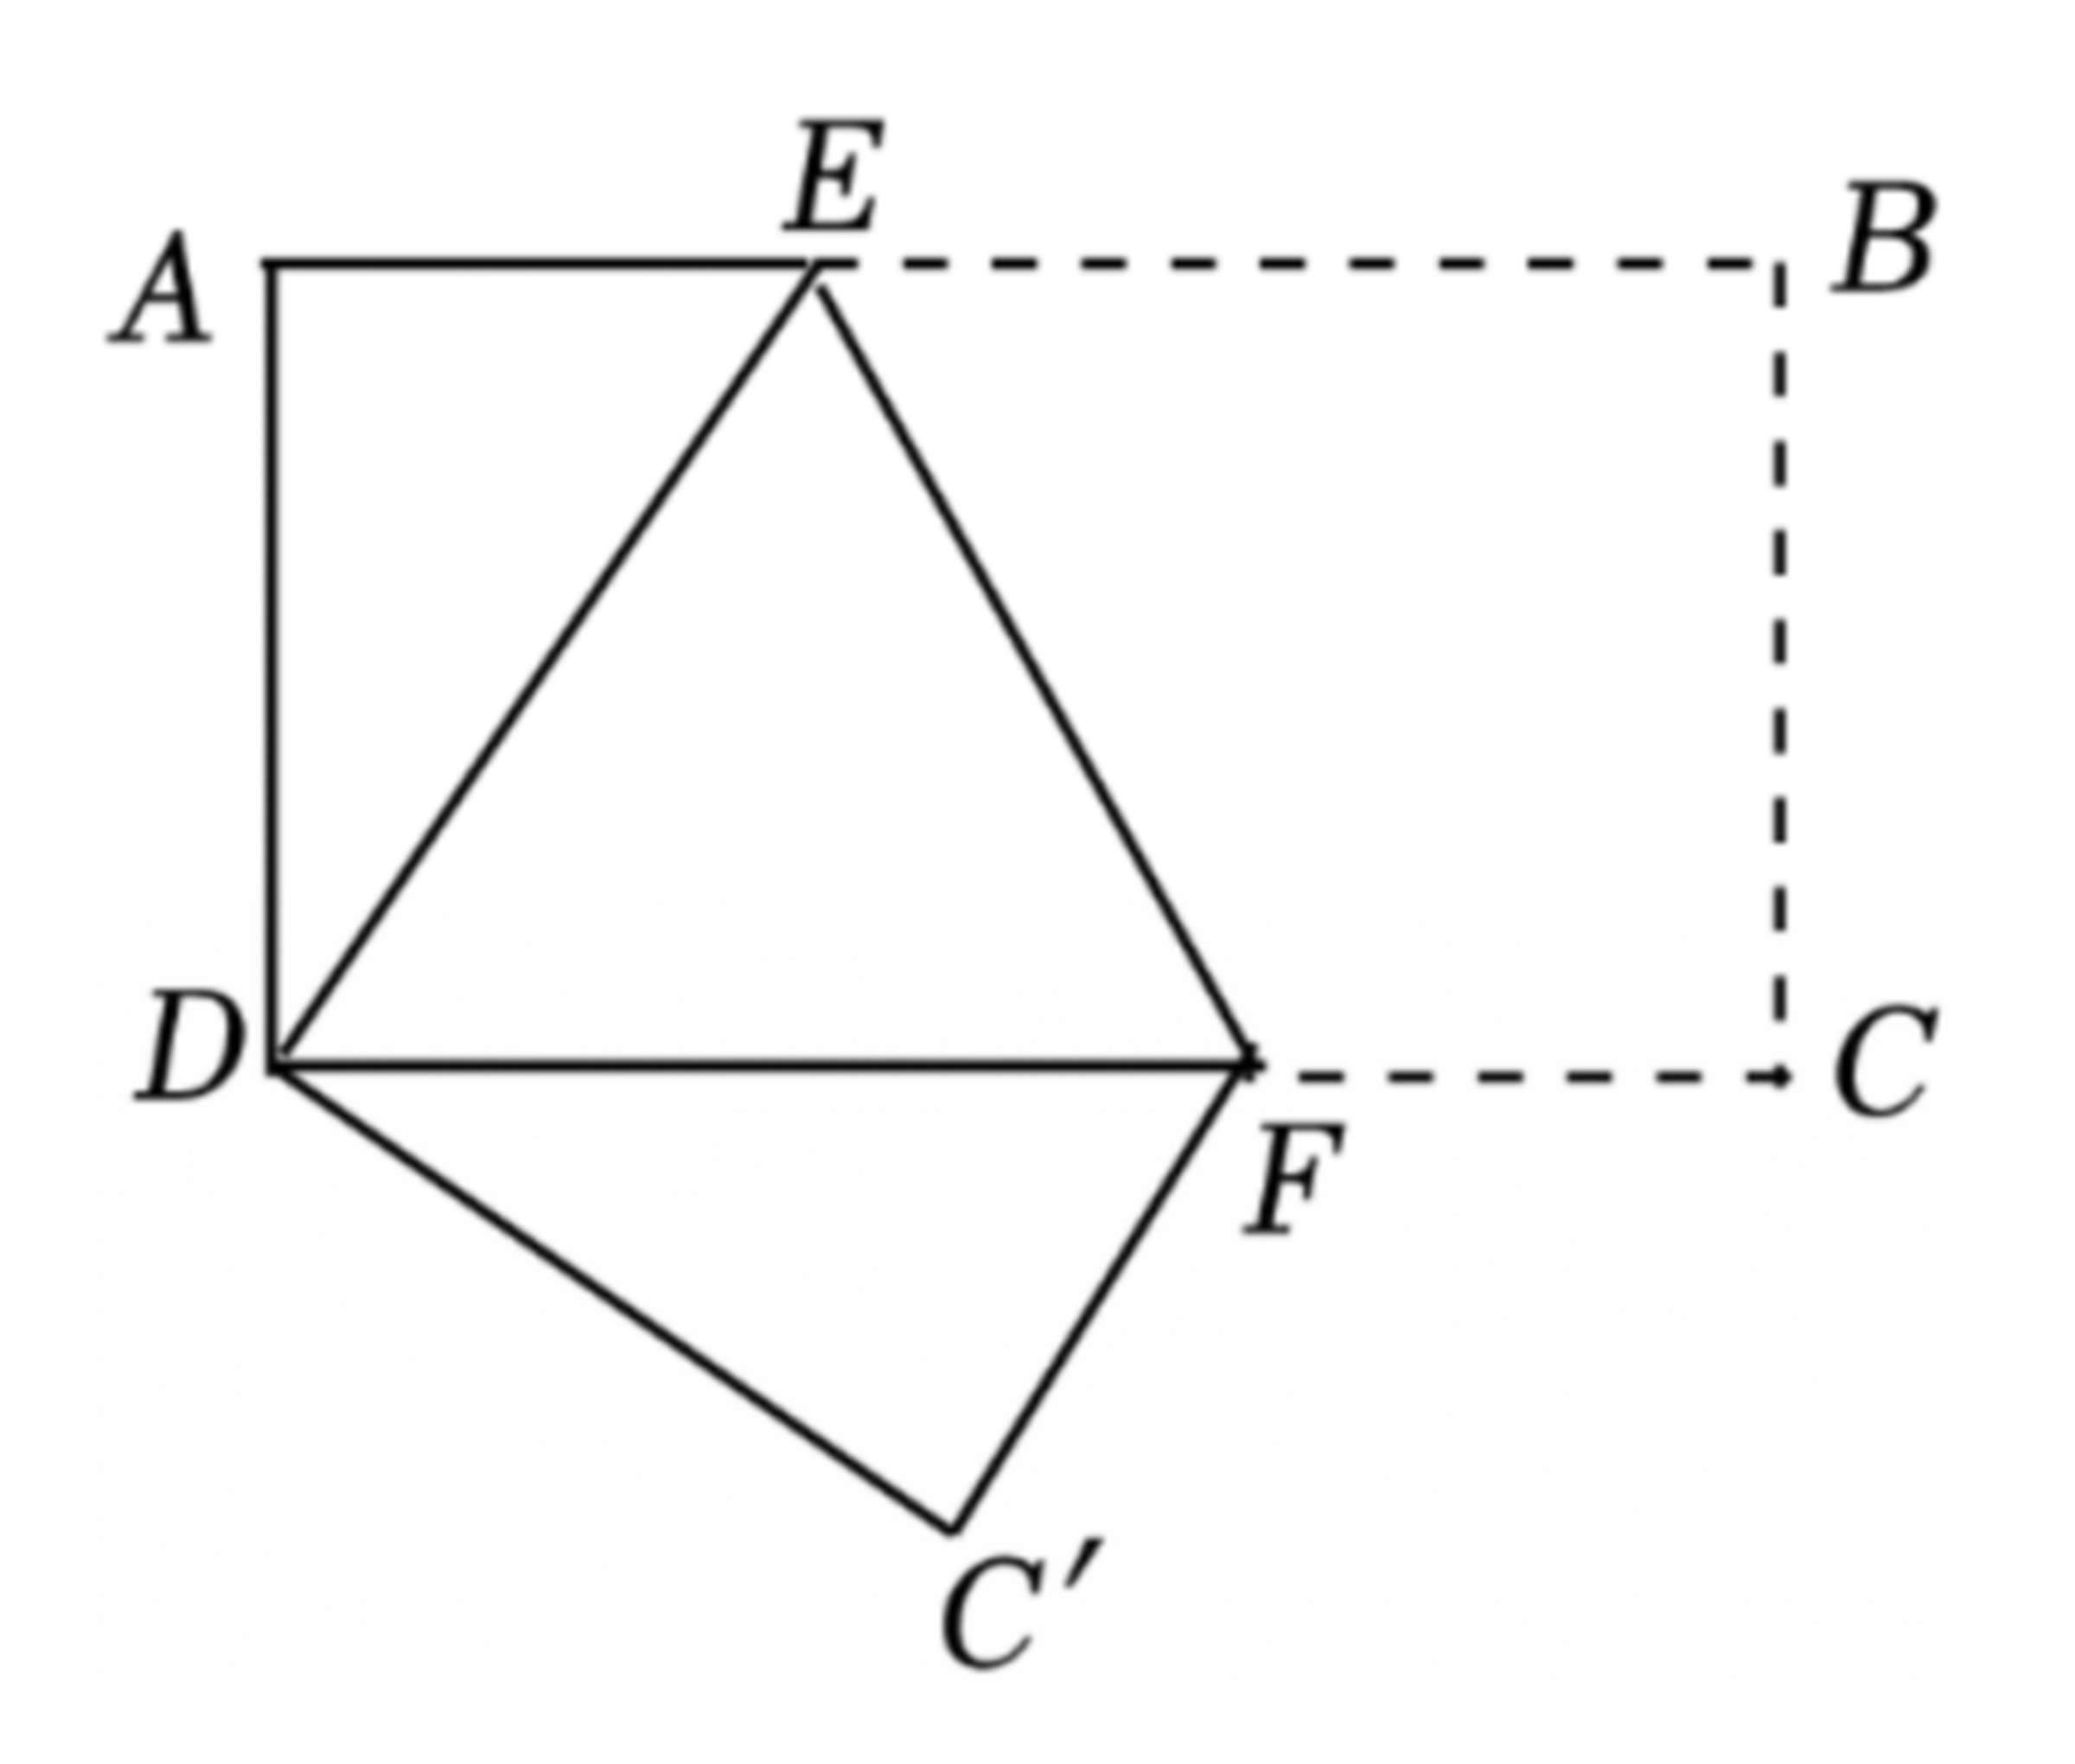
\includegraphics[width=0.40\textwidth]{figures/gao149_q11.png}
\end{center}

\ifanswer
\solbegin
\step{因为矩形 $ABCD(AB>AD)$ 的周长为 12，}
\step{在 $AB$ 和 $CD$ 边上分别取点 $E$ 和 $F$，将四边形 $BCFE$ 沿 $EF$ 折叠，}
\step{使点 $B$ 与点 $D$ 重合，此时点 $C$ 的对应点为 $C'$，}
\step{所以设 $AD=a$，$AB=b$，则 $2(a+b)=12$，}
\step{所以 $a+b=6$，且 $AB>AD$，所以 $b>a>0$，}
\step{设 $DF=x$，则 $C'F=b-x$，在 $Rt\triangle DC'F$ 中，$DC'=BC=a$，}% 几何三角形符号原卷印扁等边细线三角 $\triangle$，照录（放大 02 页确认）；$Rt$ 照录
\step{所以 $a^2+(b-x)^2=x^2$，解得 $x=\dfrac{a^2+b^2}{2b}$，}
\step{因此 $\triangle C'DF$ 的面积 $S=\dfrac{1}{2}\cdot DC'\cdot C'F=\dfrac{1}{2}\cdot a\cdot(b-x)$，}
\step{又 $b-x=b-\dfrac{(6-b)^2+b^2}{2b}=\dfrac{6(b-3)}{b}$，}
\step{所以 $S=\dfrac{1}{2}\cdot a\cdot\dfrac{6(b-3)}{b}=\dfrac{1}{2}\cdot(6-b)\cdot\dfrac{6(b-3)}{b}=\dfrac{3(6-b)(b-3)}{b}$}
\step{$=3\cdot\left(-b-\dfrac{18}{b}+9\right)$，又 $b+\dfrac{18}{b}\geqslant2\sqrt{b\cdot\dfrac{18}{b}}=6\sqrt{2}$，}
\step{当且仅当 $b=\dfrac{18}{b}$ 即 $b=3\sqrt{2}$ 时取等号，此时满足 $b>a$，}
\step{所以 $S\leqslant3\cdot(-6\sqrt{2}+9)=27-18\sqrt{2}$，故 $\triangle C'DF$ 面积的最大值为 $27-18\sqrt{2}$.}
\solend
\fi

% === Q12 === 解析内 3 幅三次函数曲线坐标图（仅答案版出）；解析 15 行（8 行 03 页＋7 行 04 页）
\item 已知 $m>0$，若存在 $t\in\R$，使得对任意 $x\in[0,m]$，不等式 $[(x-1)^2-t](x-t)\leqslant0$ 恒成立，则 $m$ 的最大值是\blankline[4.4em].

\ifanswer
\solbegin
\step{当 $t\leqslant0$ 时，$(x-1)^2-t\geqslant0$ 恒成立，}
\step{不等式 $[(x-1)^2-t](x-t)\leqslant0$ 的解集为 $x\leqslant t$，与 $x\in[0,m]$ 矛盾；}
\step{当 $t>0$ 时，不等式 $[(x-1)^2-t](x-t)\leqslant0\Leftrightarrow(x-1-\sqrt t)(x-1+\sqrt t)(x-t)\leqslant0$，}
\step{若 $t<1-\sqrt t$，即 $t\in\left(0,\dfrac{3-\sqrt5}{2}\right)$，}
\begin{center}
% 情形一 $t<1-\sqrt t$ 曲线图取 03 页右侧，去粉色水印、去色、4× LANCZOS 放大；仅答案版出
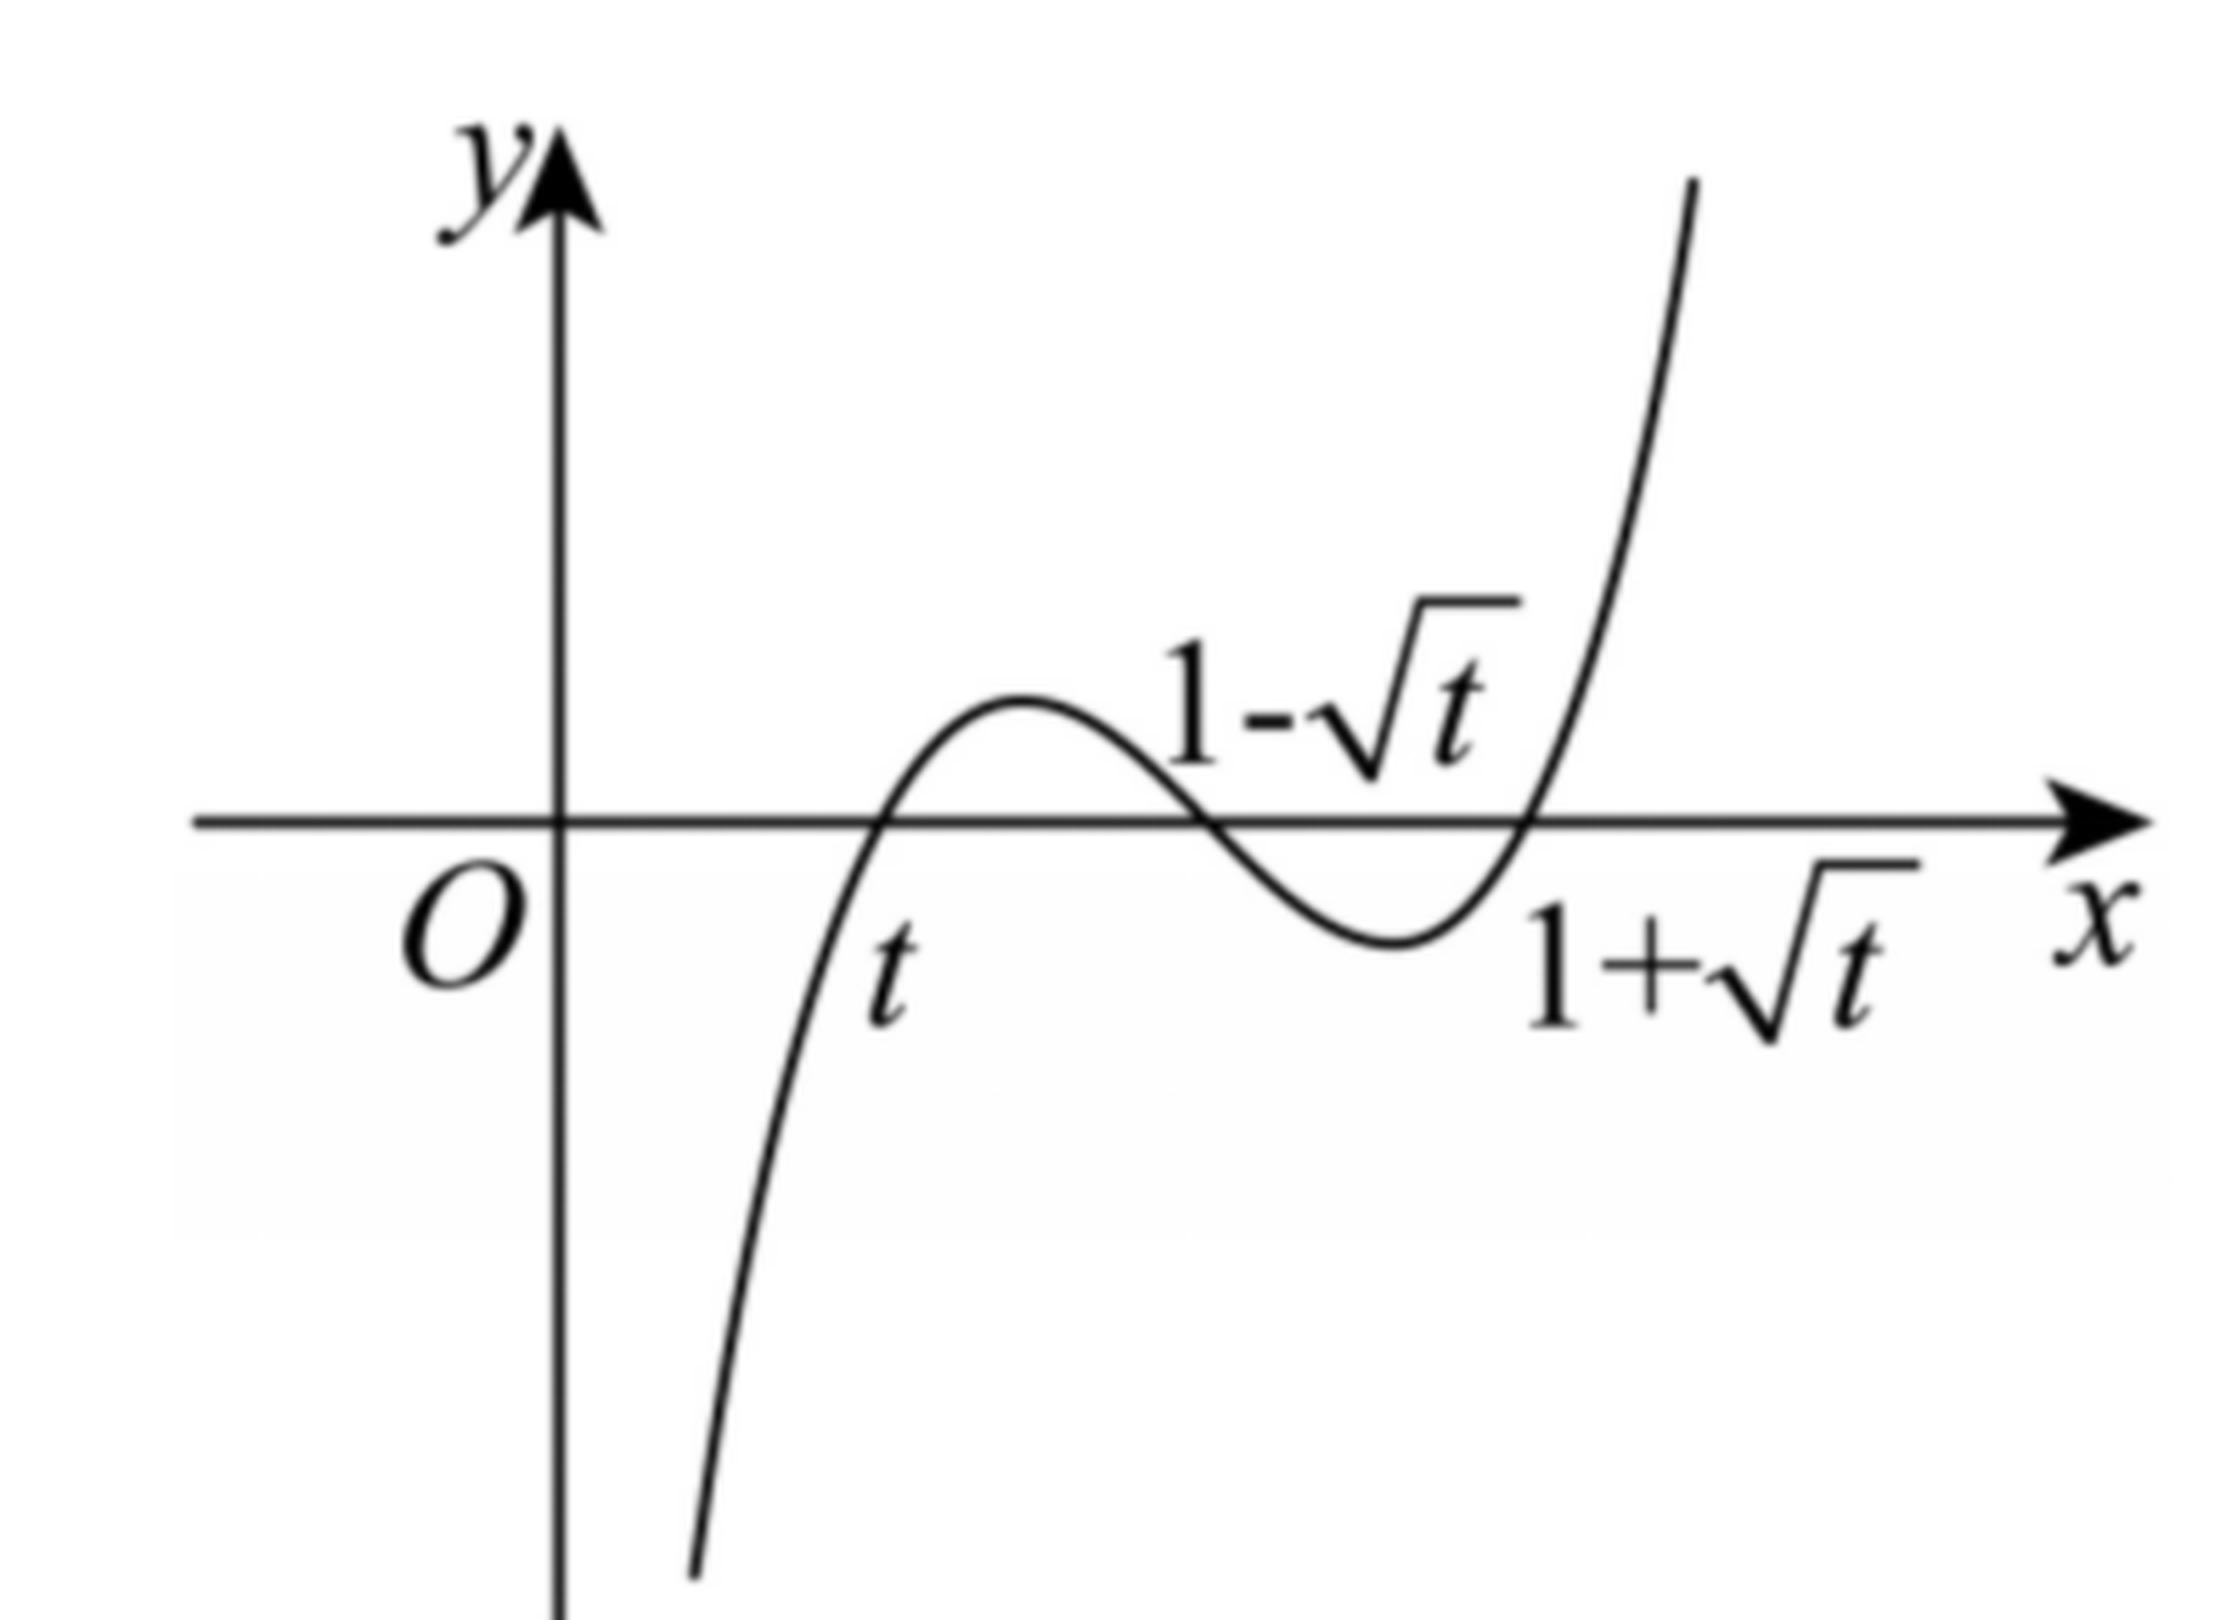
\includegraphics[width=0.40\textwidth]{figures/gao149_q12_a.png}
\end{center}
\step{则原不等式的解集为 $(-\infty,t]\cup[1-\sqrt t,1+\sqrt t]$，}
\step{当 $0<m\leqslant t$ 时，原不等式恒成立，因此}
\step{$m\in\left(0,\dfrac{3-\sqrt5}{2}\right)$；}
\step{若 $t=1-\sqrt t$，即 $t=\dfrac{3-\sqrt5}{2}$，则原不等式的解集为 $(-\infty,1+\sqrt t]$，}
\begin{center}
% 情形二 $t=1-\sqrt t$ 曲线图取 03 页右侧，去粉色水印、去色、4× LANCZOS 放大；仅答案版出
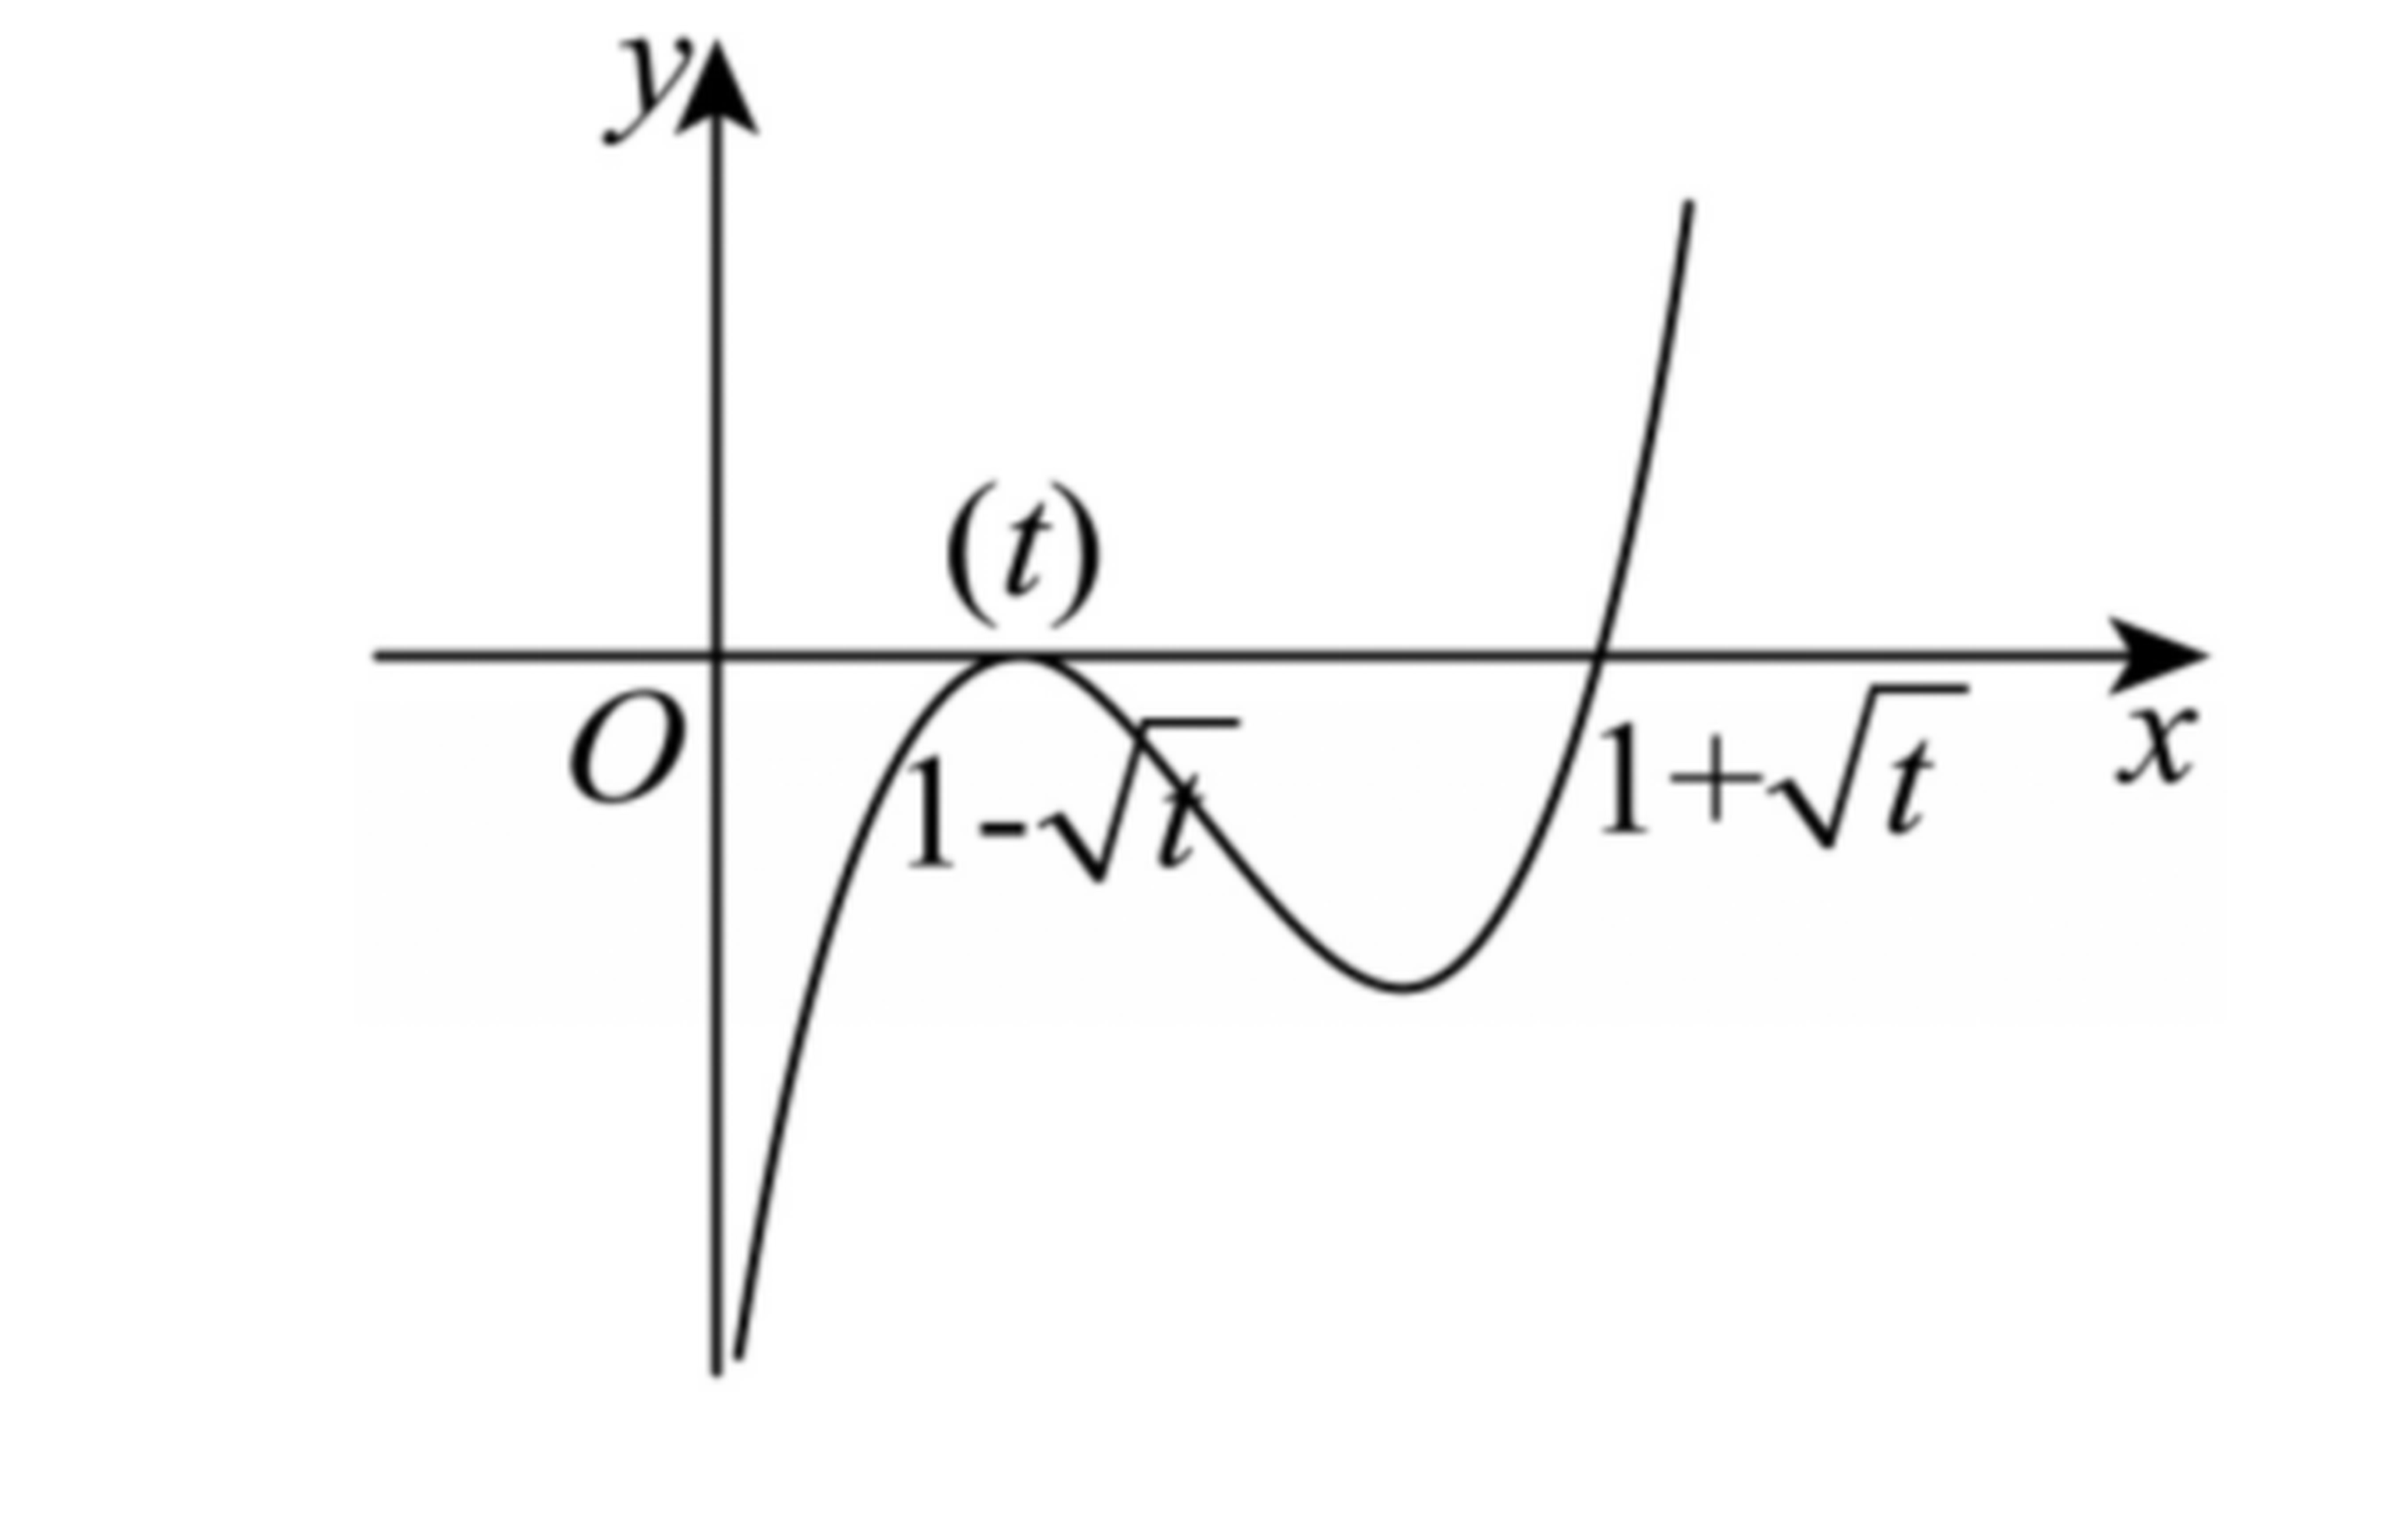
\includegraphics[width=0.40\textwidth]{figures/gao149_q12_b.png}
\end{center}
\step{当 $0<m\leqslant1+\sqrt t$ 时，原不等式恒成立，因此 $m\in\left(0,\dfrac{\sqrt5+1}{2}\right]$；}
\step{若 $1+\sqrt t>t>1-\sqrt t$，即 $t\in\left(\dfrac{3-\sqrt5}{2},\dfrac{3+\sqrt5}{2}\right)$，}
\begin{center}
% 情形三 $1+\sqrt t>t>1-\sqrt t$ 曲线图取 04 页右侧，去粉色水印、去色、4× LANCZOS 放大；仅答案版出
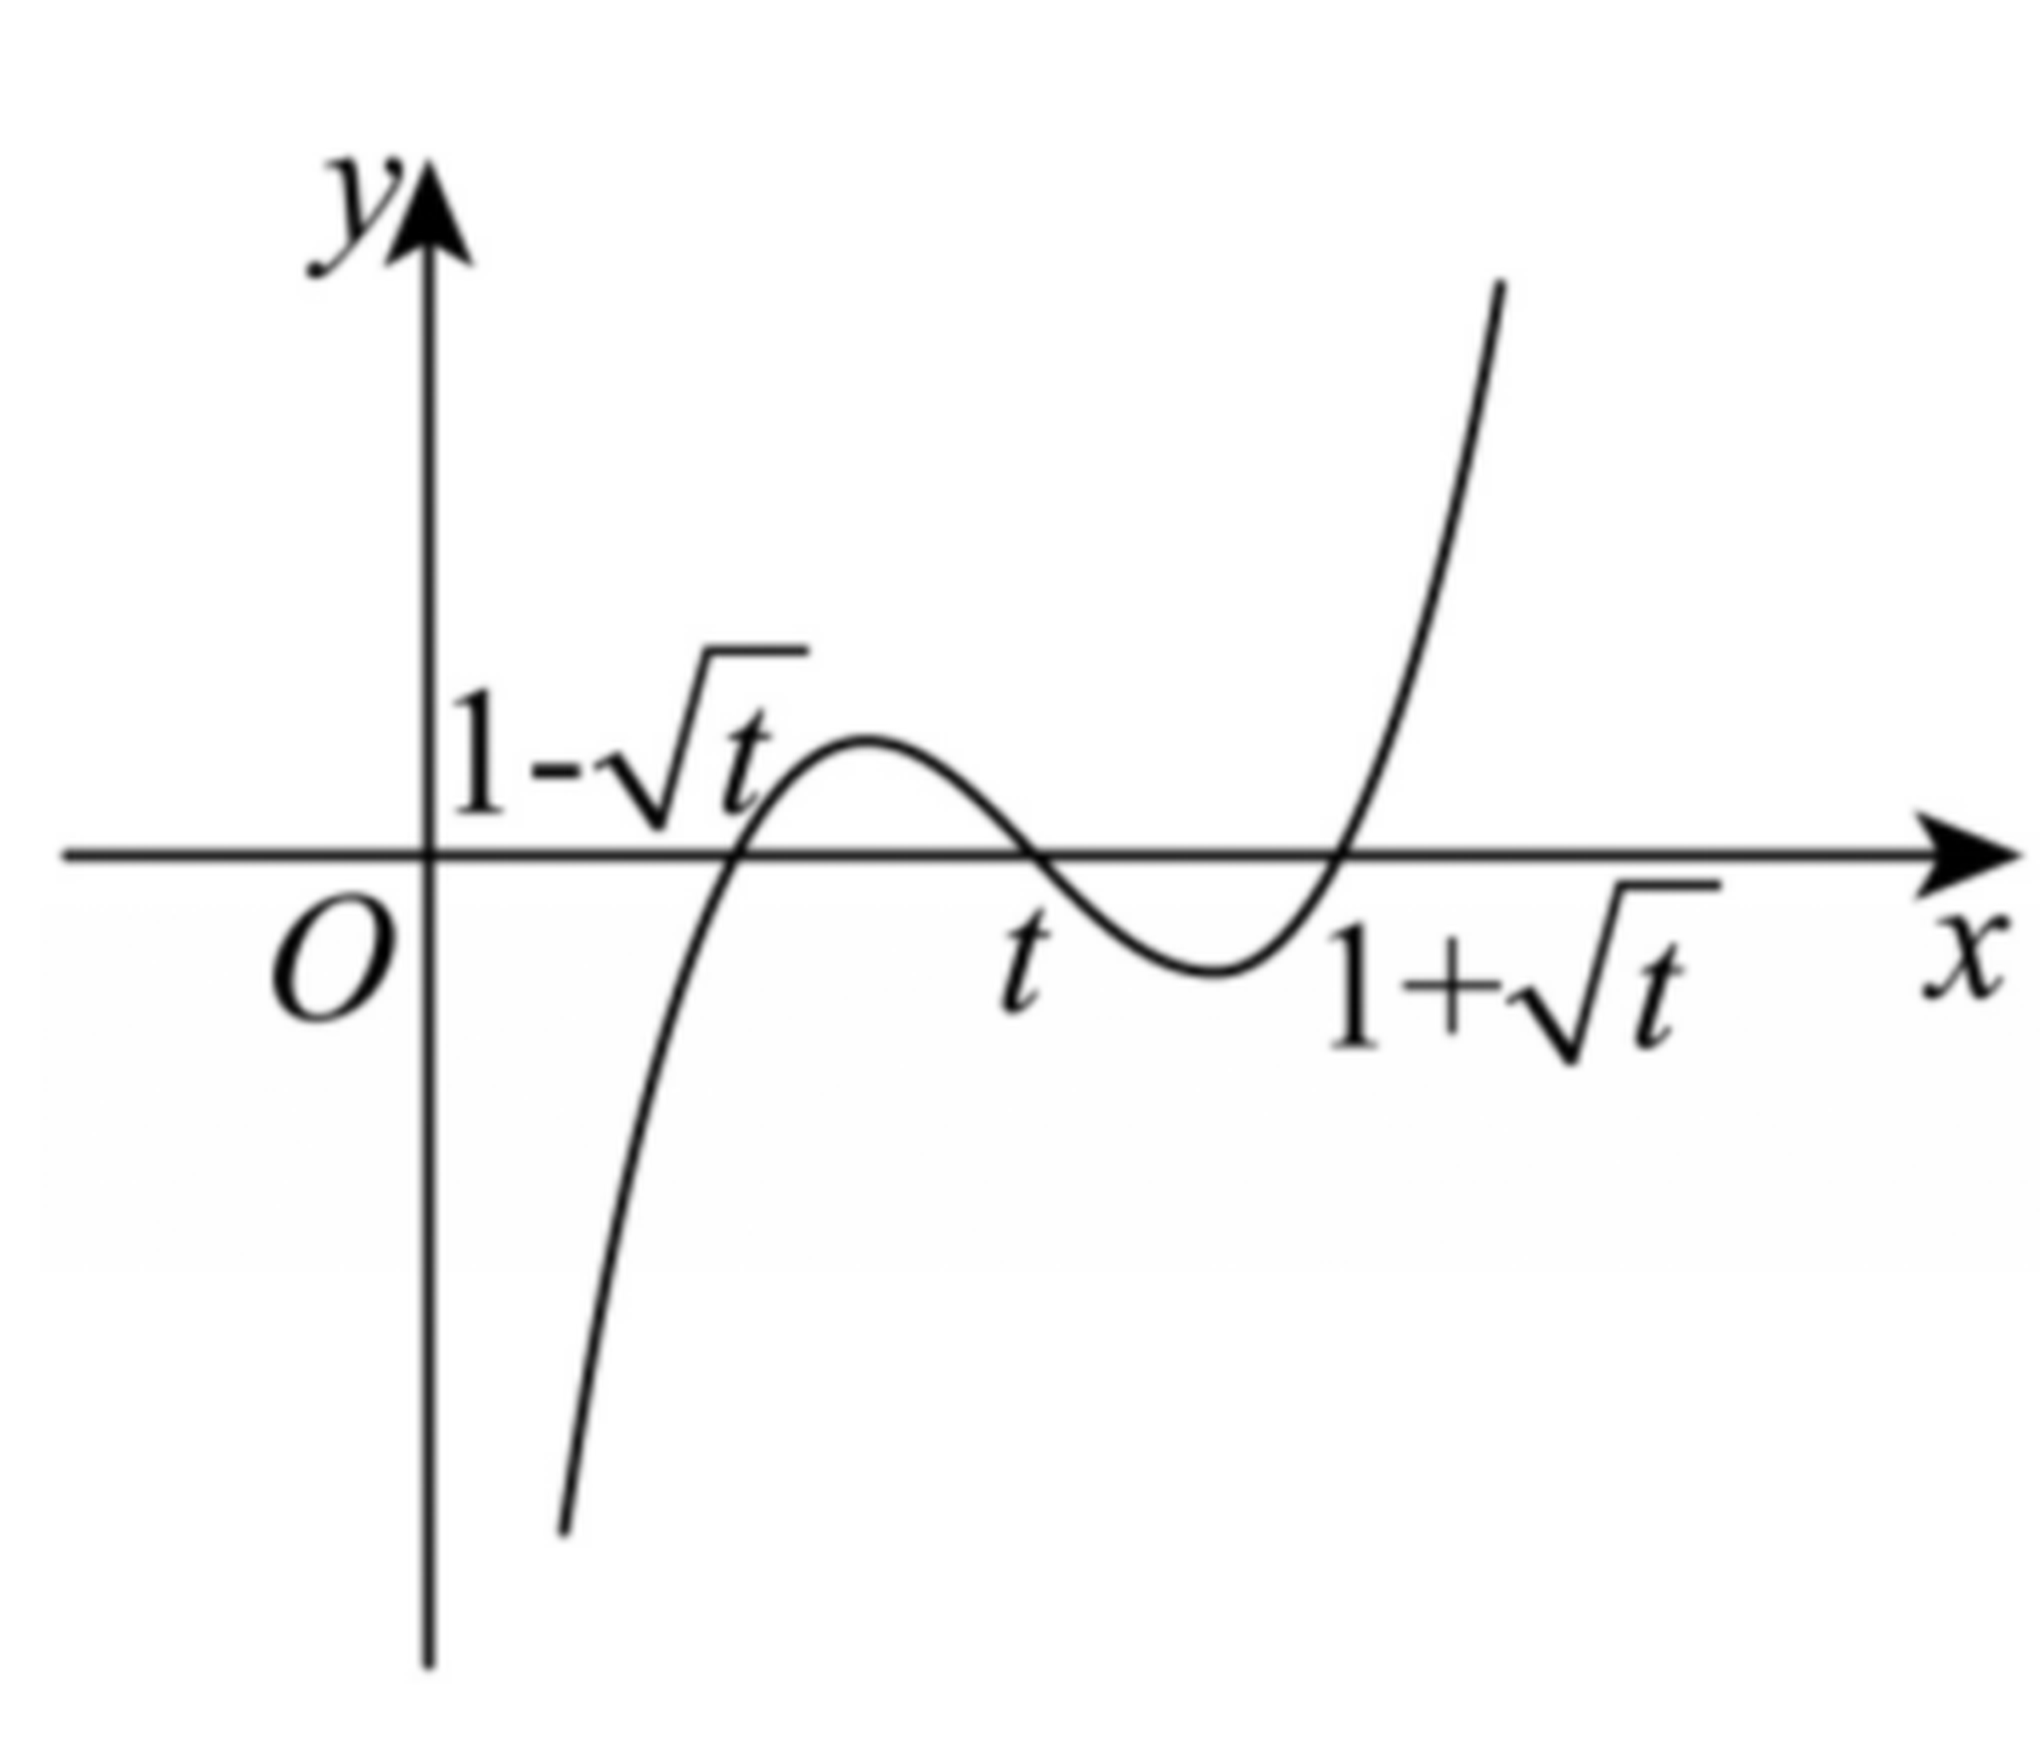
\includegraphics[width=0.40\textwidth]{figures/gao149_q12_c.png}
\end{center}
\step{则原不等式的解集为 $(-\infty,1-\sqrt t]\cup[t,1+\sqrt t]$，}
\step{当 $\begin{cases}1-\sqrt t>0\\1-\sqrt t\geqslant m\end{cases}$ 时，原不等式恒成立，此时 $t\in\left(\dfrac{3-\sqrt5}{2},1\right)$，$m\in\left(0,\dfrac{3-\sqrt5}{2}\right)$；}
\step{若 $t\geqslant1+\sqrt t$，即 $t\geqslant\dfrac{3+\sqrt5}{2}$，则取 $x=0$，$(t-1)t>0$，}
\step{原不等式不恒成立，不符合题意，}
\step{因此实数 $m$ 的取值范围是 $\left(0,\dfrac{\sqrt5+1}{2}\right]$，$m$ 的最大值是 $\dfrac{\sqrt5+1}{2}$.}
\solend
\fi

\end{enumerate}

\bigsec{二、选择题}

\begin{enumerate}
\setcounter{enumi}{12}

% === Q13 ===：答案"C"直接印在题干括号内、无【答案】/【解析】段，按 高一84 Q13／高一148 Q13 成例括号留空、另提 \ans{$C$}；四选项两行两列照原卷分行
\item 设 $ab>0$，则 $a>b$ 是 $\dfrac{1}{a}<\dfrac{1}{b}$ 的\mbox{（\quad）}

\keepwithprev
A. 充分不必要条件\qquad\qquad B. 必要不充分条件

C. 充要条件\qquad\qquad D. 既不充分又不必要条件

\ifanswer
\ans{$C$}
\fi

% === Q14 ===：$A\subset B$ 单线照录；四选项补集照原卷上划线 \overline{A}／\overline{B}；解析 1 行（由韦恩图得 B 对）
\item 已知集合 $A$、$B$ 非空，且 $A\subset B$，则下列式子中一定是空集的为\mbox{（\quad）}

\keepwithprev
A. $\overline{A}\cap B$\qquad B. $A\cap\overline{B}$\qquad C. $\overline{A}\cap\overline{B}$\qquad D. $\overline{A}\cup\overline{B}$

\ifanswer
\solbegin
\step{由韦恩图得 $B$ 对. 故选 $B$.}
\solend
\fi

% === Q15 ===："天文数字"弯引号照录；解析 2 行（首行在 04 页末、末行续 05 页顶）
\item 历史上数学计算方面的三大发明是阿拉伯数字、十进制和对数，其中对数的发明，大大缩短了计算时间，为人类研究科学和了解自然起了重大作用，对数运算对估算“天文数字”具有独特的优势. $2.5^{1000}$ 的估算值约为\mbox{（\quad）}

\keepwithprev
A. $10^{365}$\qquad B. $10^{379}$\qquad C. $10^{389}$\qquad D. $10^{398}$

\ifanswer
\solbegin
\step{$\lg 2.5^{1000}=1000\lg 2.5=1000(1-2\lg 2)\approx1000\times(1-0.602)=398$，}
\step{所以 $2.5^{1000}\approx10^{398}$. 故选 $D$.}
\solend
\fi

% === Q16 ===："完美集"新定义、圈数字①②文本模式；题干"若对任意 $x$，$y\in A$"用全角逗号、解析用顿号"$x$、$y\in A$"，两处照录不统一；解析 9 行
\item 设全集 $U=\R$，集合 $A$ 是一个非空数集，若对任意 $x$，$y\in A$，都有 $x+y\in A$、$xy\in A$，则称集合 $A$ 为一个“完美集”，给出以下命题：

①若 $A_1$、$A_2$ 都是“完美集”，且 $A_1\cap A_2\ne\varnothing$，则 $A_1\cap A_2$ 也是“完美集”；

②若 $A_1$、$A_2$ 都是“完美集”，则 $A_1\cup A_2$ 也是“完美集”.

下列说法正确的是\mbox{（\quad）}

\keepwithprev
A. ①②都是真命题\qquad\qquad B. ①是真命题，②是假命题

C. ①是假命题，②是真命题\qquad\qquad D. ①②都是假命题

\ifanswer
\solbegin
\step{由题意，全集 $U=\R$，集合 $A$ 是一个非空数集，}
\step{若对任意 $x$、$y\in A$，都有 $x+y\in A$、$xy\in A$，则称集合 $A$ 为一个“完美集”，}
\step{对于①，取 $x$、$y\in A_1\cap A_2$，则 $x\in A_1$，$x\in A_2$，$y\in A_1$，$y\in A_2$，}
\step{又 $A_1$、$A_2$ 是“完美集”，所以 $x+y\in A_1$，$xy\in A_1$，$x+y\in A_2$，$xy\in A_2$，}
\step{所以 $x+y\in A_1\cap A_2$，$xy\in A_1\cap A_2$，所以 $A_1\cap A_2$ 是“完美集”，故①正确；}
\step{对于②，取“完美集” $A_1=\{x\mid x=2k,k\in\Z\}$，$A_2=\{x\mid x=3k,k\in\Z\}$，}
\step{则 $2\in A_1$，$3\in A_2$，但 $2+3\notin A_1\cup A_2$，}
\step{即此时 $A_1\cup A_2$ 不是“完美集”，故②错误.}
\step{故选 $B$.}
\solend
\fi
\end{enumerate}

\bigsec{三、解答题}

\begin{enumerate}
\setcounter{enumi}{16}

% === Q17 ===："图像"（有亻）照录（Q17 题干与解析共 2 处）；绝对值 \lvert…\rvert；解析 7 行
\item 已知 $m\in\R$，$f(x)=(m^2-m-5)x^m$. 若 $y=f(x)$ 是幂函数，且其图像不经过原点.

(1) 求实数 $m$ 的值；

(2) 若 $f(a)=f(b)$ 且 $a\ne b$，求 $\lvert a+2\rvert+\lvert b-1\rvert$ 的最小值，并指出取到最小值时 $a$ 的取值范围.

\ifanswer
\solbegin
\step{(1) $f(x)=(m^2-m-5)x^m$ 是幂函数，得 $m^2-m-5=1$，即 $m^2-m-6=0$，}
\step{解得 $m=-2$ 或 $m=3$，又函数图像不经过原点，所以 $m=-2$($3$ 舍)；}
\step{(2) 由 (1) 得 $f(x)=x^{-2}=\dfrac{1}{x^2}$ 为偶函数，}
\step{$x<0$ 时，函数 $f(x)$ 严格增，$x>0$ 时，函数 $f(x)$ 严格减，}
\step{又 $f(a)=f(b)$ 且 $a\ne b$，所以 $a=-b$，且 $a\ne0$，$b\ne0$，}
\step{则 $\lvert a+2\rvert+\lvert b-1\rvert=\lvert a+2\rvert+\lvert-a-1\rvert=\lvert a+2\rvert+\lvert a+1\rvert$，}
\step{则 $\lvert a+2\rvert+\lvert b-1\rvert$ 的最小值为 $1$，取到最小值时 $a$ 的取值范围是 $[-2,-1]$.}
\solend
\fi

% === Q18 ===：判别式两形混用——(1) cases 块印高 \Delta、(2) 独立行印扁 \triangle，逐处照录不统一；解析 8 行
\item 已知命题 $p$：方程 $x^2+4x+m-1=0$ 有两个不等的负根；命题 $q$：方程 $4x^2+4x+m-2=0$ 无实根.

(1) 若 $p$ 为真命题，求 $m$ 的取值范围；

(2) 若 $p$、$q$ 两命题一真一假，求 $m$ 的取值范围.

\ifanswer
\solbegin
\step{(1) 若 $p$ 为真命题，即方程 $x^2+4x+m-1=0$ 有两个不等的负根；}
\step{必有 $\begin{cases}\Delta=16-4(m-1)>0\\m-1>0\end{cases}$，解得 $1<m<5$，即 $m$ 的取值范围为 $(1,5)$；}
\step{(2) 命题 $q$：方程 $4x^2+4x+m-2=0$ 无实根，}
\step{则有 $\triangle=16-16(m-2)<0$，解得 $m>3$，}
\step{若 $p$ 和 $q$ 有且只有一个为真命题，}
\step{若 $p$ 真 $q$ 假，必有 $\begin{cases}1<m<5\\m\leqslant3\end{cases}$，则有 $1<m\leqslant3$，}
\step{若 $p$ 假 $q$ 真，必有 $\begin{cases}m\leqslant1\text{ 或 }m\geqslant5\\m>3\end{cases}$，则有 $m\geqslant5$，}
\step{综上，$1<m\leqslant3$ 或 $m\geqslant5$.}
\solend
\fi

% === Q19 ===：$A\subseteq B$ 带下划线照录；解析 7 行（(2) 两组 cases 并排）
\item 已知 $m\in\R$，集合 $A=\left\{x\mid y=\sqrt{3-x}-\dfrac{1}{\sqrt{x-1}}\right\}$，集合 $B=\{x\mid 2m\leqslant x\leqslant1-m\}$.

(1) 若 $A\cup B=B$，求实数 $m$ 的取值范围；

(2) 若 $A\cap B=\varnothing$，求实数 $m$ 的取值范围.

\ifanswer
\solbegin
\step{(1) 函数 $y=\sqrt{3-x}-\dfrac{1}{\sqrt{x-1}}$，则 $\begin{cases}3-x\geqslant0\\x-1>0\end{cases}$，解得 $1<x\leqslant3$，}
\step{所以 $A=\{x\mid1<x\leqslant3\}$，}
\step{因为 $A\cup B=B$，所以 $A\subseteq B$，则 $\begin{cases}2m\leqslant1\\1-m\geqslant3\end{cases}$，解得 $m\leqslant-2$，}
\step{综上，实数 $m$ 的取值范围为 $(-\infty,-2]$；}
\step{(2) 当 $B=\varnothing$ 时，则 $2m>1-m$，解得 $m>\dfrac{1}{3}$，}
\step{当 $B\ne\varnothing$ 时，则 $\begin{cases}2m\leqslant1-m\\2m>3\end{cases}$ 或 $\begin{cases}2m\leqslant1-m\\1-m\leqslant1\end{cases}$，解得 $m\in\varnothing$ 或 $0\leqslant m\leqslant\dfrac{1}{3}$，}
\step{综上，实数 $m$ 的取值范围为 $[0,+\infty)$.}
\solend
\fi

% === Q20 ===：n 阶基本不等式推广；(3) 解析含 \overbrace{…}^{k} 上括号；(2) 解析"x=x=x=3(1-x)"三连等系原卷笔误、照录加注（见 ⑤）；解析 14 行
\item 教材中的基本不等式可以推广到 $n$ 阶：$n$ 个正数的算术平均数不小于它们的几何平均数，即对于任意的正数 $a_1$、$a_2$、$\cdots$、$a_n$，有 $\dfrac{a_1+a_2+\cdots+a_n}{n}\geqslant\sqrt[n]{a_1\cdot a_2\cdots a_n}$（$n\in\N$ 且 $n\geqslant2$），且等号当且仅当 $a_1=a_2=\cdots=a_n$ 时成立. 利用此结论解决下列问题：

(1) 若 $x$、$y$、$z>0$，求 $\dfrac{y}{x}+\dfrac{2z}{y}+\dfrac{4x}{z}$ 的最小值；

(2) 已知 $0<x<1$，求 $x^3(1-x)$ 的最大值，并求取得最大值时的 $x$ 的值；

(3) 对任意的正整数 $k$，判断 $\left(1+\dfrac{1}{k}\right)^k$ 与 $\left(1+\dfrac{1}{k+1}\right)^{k+1}$ 的大小关系，并证明.

\ifanswer
\solbegin
\step{(1) 因为 $x$、$y$、$z>0$，有 $\dfrac{y}{x}>0$，$\dfrac{2z}{y}>0$，$\dfrac{4x}{z}>0$}
\step{所以 $\dfrac{y}{x}+\dfrac{2z}{y}+\dfrac{4x}{z}\geqslant3\sqrt[3]{\dfrac{y}{x}\cdot\dfrac{2z}{y}\cdot\dfrac{4x}{z}}=3\sqrt[3]{8}=6$，}
\step{当且仅当 $\dfrac{y}{x}=\dfrac{2z}{y}=\dfrac{4x}{z}$ 时取等号，故 $\dfrac{y}{x}+\dfrac{2z}{y}+\dfrac{4x}{z}$ 的最小值为 $6$.}
\step{(2) 因为 $0<x<1$，所以 $1-x>0$，}
\step{$x^3(1-x)=\dfrac{1}{3}[x\cdot x\cdot x\cdot3(1-x)]\leqslant\dfrac{1}{3}\left[\dfrac{x+x+x+3(1-x)}{4}\right]^4=\dfrac{1}{3}\times\left(\dfrac{3}{4}\right)^4$}
\step{$=\dfrac{27}{256}$，当且仅当 $x=x=x=3(1-x)$，即 $x=3(1-x)$，$x=\dfrac{3}{4}$ 取等号，}% 原卷"x=x=x=3(1-x)"三连等，疑为四因子相等之误排，放大 08 页确认，照录未改（见 ⑤）
\step{所以 $0<x<1$ 时，$x^3(1-x)$ 的最大值是 $\dfrac{27}{256}$，取最大值时 $x=\dfrac{3}{4}$.}
\step{(3) 对任意 $k\in\N^*$，$\left(1+\dfrac{1}{k}\right)^k<\left(1+\dfrac{1}{k+1}\right)^{k+1}$.}
\step{证明：$\left(1+\dfrac{1}{k}\right)^k=\overbrace{\left(1+\dfrac{1}{k}\right)\cdot\left(1+\dfrac{1}{k}\right)\cdots\left(1+\dfrac{1}{k}\right)}^{k}\times1$}
\step{$\leqslant\left(\dfrac{\overbrace{\left(1+\dfrac{1}{k}\right)+\left(1+\dfrac{1}{k}\right)+\cdots+\left(1+\dfrac{1}{k}\right)}^{k}+1}{k+1}\right)^{k+1}$}
\step{$=\left(\dfrac{\overbrace{(1+1+\cdots+1)}^{k}+\overbrace{\left(\dfrac{1}{k}+\dfrac{1}{k}+\cdots+\dfrac{1}{k}\right)}^{k}+1}{k+1}\right)^{k+1}=\left(\dfrac{k+1+1}{k+1}\right)^{k+1}=\left(1+\dfrac{1}{k+1}\right)^{k+1}$，}
\step{当且仅当 $1+\dfrac{1}{k}=1$ 时取等号，}
\step{但是任意 $k\in\N^*$ 时 $1+\dfrac{1}{k}>1$，所以等号不成立，}
\step{故任意 $k\in\N^*$ 时，$\left(1+\dfrac{1}{k}\right)^k<\left(1+\dfrac{1}{k+1}\right)^{k+1}$.}
\solend
\fi

% === Q21 ===："减 k 集"新定义（引号内 k／数字两侧空格照录）；解析 26 行（续 10 页），含 ⑤ 三处原卷笔误照录
\item 定义：对于给定的整数 $k$，若非空集合 $A$ 满足如下 3 个条件：

① $A$ 是正整数集的子集；② $A\ne\{1\}$；

③对任意正整数 $x,y$，若 $x+y\in A$，则 $xy-k\in A$；则称集合 $A$ 为“减 $k$ 集”.

(1) 判断集合 $A=\{1,2\}$ 是否为“减 $0$ 集”？是否为“减 $1$ 集”？（无需说明理由）

(2) 证明：不存在“减 $2$ 集”；

(3) 是否存在“减 $1$ 集”？如果存在，求出所有“减 $1$ 集”；如果不存在，说明理由.

\ifanswer
\solbegin
\step{(1) 因为 $P\subseteq\N^*$，$P\ne\{1\}$，$1+1=2\in P$，$1\times1-0\in P$，}
\step{所以集合 $P=\{1,2\}$ 是“减 $0$ 集”；}
\step{因为 $P\subseteq\N^*$，$P\ne\{1\}$，$1+1=2\in P$，$1\times1-1\notin P$，}
\step{所以集合 $P=\{1,2\}$ 是“减 $1$ 集”；}% 按条件③应为"不是"，原卷径印"是"，放大 09 页确认，照录未改（见 ⑤）
\step{(2) 假设存在集合 $A$ 是“减 $2$ 集”，若 $x+y\in A$，则 $xy-2\in A$，}
\step{①当 $x+y=xy-2$ 时，有 $(x-1)(y-1)=3$，}
\step{则 $x$、$y$ 一个为 $2$，一个为 $4$，所以集合 $A$ 有元素 $6$，}
\step{但 $3+3\in A$，$3\times3-2\notin A$，与 $A$ 是“减 $2$ 集”矛盾；}
\step{②当 $x+y\ne xy-2$ 时，则 $x+y=xy-1$ 或 $x+y=xy-m$($m>2$)，}
\step{若 $x+y=xy-1$，$m=1$ 时，$M$ 为除 $1$ 以外的最小元素，}% 原卷"m=1"上文未显式定义，疑笔误，放大 09 页确认，照录未改（见 ⑤）
\step{则 $x=M-1$，$y=1$ 时，$xy-2=M-3$ 小于 $M$，}
\step{要符合题意，必须 $M=4$，}
\step{此时取 $x-2$，$y=2$，$xy-2=2$ 不属于 $A$，故不符合题意，}% 原卷"取 x−2"疑为"取 x=2"误排，放大 09 页确认，照录未改（见 ⑤）
\step{当 $m>2$ 时，$(x-1)(y-1)=m+1$，同样得出矛盾，}
\step{综上，不存在 $A$ 是“减 $2$ 集”.}
\step{(3) 存在“减 $1$ 集” $A$，则 $A\ne\{1\}$，}
\step{①假设 $1\in A$，则 $A$ 中除了元素 $1$ 以外，必然还含有其它元素，}
\step{假设 $2\in A$，$1+1\in A$，而 $1\times1-1\notin A$，所以 $2\notin A$，}
\step{假设 $3\in A$，$1+2\in A$，而 $1\times2-1\in A$，所以 $3\in A$，}
\step{所以 $A=\{1,3\}$，}
\step{假设 $4\in A$，$1+3\in A$，而 $1\times3-1\notin A$，所以 $4\notin A$，}
\step{假设 $5\in A$，$1+4\in A$，$1\times4-1\in A$，$2+3=5$，$2\times3-1\in A$，所以 $5\in A$，}
\step{所以 $A=\{1,3,5\}$，}
\step{以此类推，得 $A=\{1,3,5,\cdots,2n-1,\cdots\}$，($n\in\N^*$)，}
\step{所以所有的“减 $1$ 集”有 $\{1,3\}$，$\{1,3,5\}$，$\{1,3,5,7\}$，$\cdots$，$\{1,3,5,\cdots,2n-1,\cdots\}$，}
\step{$(n\in\N^*)$.}
\solend
\fi
\end{enumerate}

\end{document}
"
%
% ① 原始材料：微信公众号"魔都数学加油站"文章，连载"27学年高一149"，原文标题
% "27学年高一149——2026-2027年上海市青浦高级中学上外云间高一上期中"；
% 原文链接：https://mp.weixin.qq.com/s/T7_nyoR1k0o_5og7FkDsyw 。
% 正文为 10 张 PNG 页（01/02/03/04/10 为 2560×3620，05/06/07/08/09 为 4762×6735，
% 同一篇各页分辨率混排，逐页按各自分辨率裁图核对，别按预览比例换算裁框）。
% 体例：混合体例讲评版——19 题中 Q6 只印【答案】、无【解析】；Q13 的答案"C"
%   直接印在题干括号内、无【答案】/【解析】段；其余 17 题印【解析】（逐题核实，见 ② ②）。
% 题目、答案、解析均据原图转录；卷面粉红色水印"魔都数学加油站"及公众号页脚未录入。
% 全卷插图清单（逐页通读 10 页确认）：1 幅题目配图 + 3 幅【解析】内配图：
%   · Q11 矩形 ABCD 折叠几何图（02 页右侧：A/B/C/D/E/F/C' 与虚线 EB、BC、FC），
%     题干"如图"处，题目配图、三版都出，裁 figures/gao149_q11.png；
%   · Q12【解析】内 3 幅三次函数曲线坐标图（03 页右侧两幅 + 04 页右侧一幅：
%     x/y 轴、O、t、1-\sqrt t、1+\sqrt t 等标注，分别对应 t<1-\sqrt t、
%     t=1-\sqrt t、1+\sqrt t>t>1-\sqrt t 三种情形），解析配图、仅答案版出，
%     分别裁 figures/gao149_q12_a.png／_b.png／_c.png，放 \ifanswer 内 \step 之间
%     （高一73 第 16 题成例）；
%   其余各页逐页确认无其它题目配图、无表格；Q14 解析"由韦恩图得 B 对"仅文字推导、
%   原卷并未印韦恩图；Q9／Q18／Q19 的 cases 块与 Q20(3) 的 \overbrace 为数学块（非图）；
%   10 页下半仅水印、无正文。4 图均取自原卷截图，去粉色水印、去色、4× LANCZOS 放大。
%
% 卷首标题：原卷印作"2026-2027 年青浦高级中学上外云间高一上期中"，年份区间按全稿
% 惯例排 en dash；原卷卷面未印副标题，本稿按同期中卷（高一140／141／143／144／145／
% 146／147／148）知识模块口径补出"集合与常用逻辑用语、不等式、函数"。
%
% 题号体例（逐页核实定稿）：本卷共 19 题——一、填空题 3—12（10 题）、
% 二、选择题 13—16（4 题）、三、解答题 17—21（5 题）。
% 三节分别 \setcounter{enumi}{2}／{12}／{16}。原卷从第 3 题起、无第 1、2 题，
% 本稿保留原题号；全卷无附加题节（Q21 解析末行"（n\in N^*）."为全卷收尾）。
%
% ② 与原卷的排版差异：
%   ① 原文从第 3 题起，本稿保留原题号；共 19 题三节；
%   ② 混合体例逐题核实：Q6（反证法"假设的内容"）只印【答案】、无【解析】，
%      按 高一140 第 5 题／高一145 Q3 成例提 \ans{}、不补造解析；Q13 答案"C"直接
%      印在题干括号内、全卷无该题【答案】/【解析】段，按 高一84 Q13／高一148 Q13
%      成例括号 \mbox{（\quad）} 留空、另提 \ans{$C$}；其余 17 题印【解析】、
%      用 \solbegin…\solend，选择题答案在解析末句"故选 X"（Q14 选 B、Q15 选 D、
%      Q16 选 B，逐个放大 04/05 页核实）、题干括号留空、不另提 \ans{}；
%      答案版【答案】/【解析】标记数 = 19（2 个 \ans ＋ 17 个 \solbegin）
%      = 全卷题数；
%   ③ 原卷卷面未印副标题，本稿按知识模块口径补出；
%   ④ 原卷填空横线按全稿惯例排 \blankline[4.4em]；选择题括号排 \mbox{（\quad）}、
%      选项段前按惯例加 \keepwithprev；Q13／Q16 四选项为两行两列、Q14／Q15
%      选项为一行，照原卷分行；解答题不留作答区、不加 \anspace（原卷为讲评版）；
%   ⑤ 数集：Q6"a,b\in N"、Q8"x\in R"、Q9"a\in R"／"解集为 R"、Q12"t\in R"、
%      Q16"U=R"、Q17"m\in R"、Q19"m\in R"、Q20"n\in N" 原卷印斜体 R/N，
%      按全稿惯例统一改 \R／\N；Q20(3)、Q21 的 $N^*$ 排 \N^*；Q16 解析
%      "$k\in Z$" 排 \Z。绝对值排 \lvert…\rvert（Q17），集合描述竖线排 \mid
%      （Q19、Q16 解析）；不等号按全稿惯例排 \leqslant／\geqslant；
%      补集照原卷上划线排 \overline{A}／\overline{B}（Q14 四选项）；空集
%      \varnothing（Q16、Q19、Q21）；
%   ⑥ 子集符号逐处照录不统一：Q4 题干"{1,2}⊆A⊂{1,2,3,4,5,6}" 前者印带下划线
%      ⊆、照录 \subseteq，后者印单线 ⊂、照录 \subset；Q10"A⊆{-1,1/2,2,3}"、
%      Q19 解析"A⊆B"、Q21 解析"P⊆N*" 均印带下划线 ⊆、照录 \subseteq；
%      Q14"A⊂B" 印单线 ⊂、照录 \subset（逐处放大 01/02/04/07/09 页确认，见 ④）；
%   ⑦ 子题标号 (1)(2)(3) 半角括号照录；圈数字 ①②③ 在文本模式（Q16 两命题、
%      Q21 三个条件与解析的①②）按 common.sty 划入 CJK 字符类渲染；cases 块整体
%      算一个印刷行；\left…\right 不得拆到不同 $…$ 组；数学式内 CJK 用 \text{}
%      （Q18 解析 cases 块"\text{或}"）；Q11 解析"Rt\triangle DC'F" 的 Rt 照录；
%   ⑧ 题干／解析中的中文弯引号按原卷照录：Q6" 已知 a,b\in N，若 ab 能被 5 整除，
%      那么 a、b 中至少有一个能被 5 整除 "（开引号后紧跟"已知"、闭引号后空格接"时"）、
%      Q15"天文数字"、Q16"完美集"、Q21"减 k 集""减 0 集""减 1 集""减 2 集"
%      （引号内 k／数字两侧有空格），注释内一律 ASCII 引号；
%   ⑨ 半角逗号在数学组之间是全稿惯例、非笔误（Q8"$a>0,a\ne1,x\in\R$"、
%      Q21 题干"$x,y$" 等），逐处照录别改；Q16 题干"若对任意 $x$，$y\in A$"
%      用全角逗号而解析用顿号"$x$、$y\in A$"，两处不同均照录；行末西文句点
%      照录为 ASCII `.`；行中全角逗号／顿号照录；
%   ⑩ "图像／图象"逐处放大核：Q10 题干与解析共 6 处均印"图象"（象，无亻）；
%      Q17 题干"其图像不经过原点"与解析"又函数图像不经过原点" 2 处印"图像"
%      （像，有亻），逐处照录未统一改动（放大 02/05/06 页确认）；
%   ⑪ 判别式 Δ/△ 混用是照录项：Q9 解析 cases 块"Δ=4(a−2)²+16(a−2)<0"、
%      Q18(1) cases 块"Δ=16−4(m−1)>0" 两处印等腰偏高粗三角 \Delta；
%      Q18(2) 独立行"△=16−16(m−2)<0" 印扁等边细线三角 \triangle，
%      逐处放大判断、照录不统一（参照 高一142／144／145／146／148 头注④口径）；
%      另 Q11 题干"△C'DF 面积"与解析 3 处"△"（含"Rt△DC'F"）共 4 处几何
%      三角形符号亦印扁细线三角，照录 \triangle（非判别式，字形同类，见 ④）；
%   ⑫ 一条 \step = 原卷解析的一个印刷行，cases 块整体算一个印刷行；别把原卷折行
%      并起来、别把一行拆多条。Q11 十三行（7 行在 02 页＋6 行在 03 页）、
%      Q12 十五行（8 行在 03 页＋7 行在 04 页）、Q16 九行、Q21 二十六行
%      （续 10 页）均按印刷行逐条断，不丢行；
%   ⑬ 配图：Q11 题目配图（三版都出）放 \item 内题干之后 \begin{center}，
%      大图块加 \needvspace{8cm} 守卫把整块推走（守卫放 \item 之前，见
%      高一145 Q14/Q20 成例与切页审计 B 类坑）；Q12 三幅解析配图（仅答案版出）
%      放 \ifanswer 内 \solbegin…\solend 的 \step 之间；三版切页审计均"合计异常：无"；
%   ⑭ 跨页续印按题合并：Q3/4/5 在 01 页；Q6/7/8 题干与解析在 01 页；
%      Q9 题干在 01 页末、解析 4 行在 02 页顶；Q10 题干＋解析在 02 页；
%      Q11 题干＋图＋解析前 7 行在 02 页、解析后 6 行续 03 页顶；
%      Q12 题干＋解析首行在 03 页末、解析续 7 行在 03 页下半＋7 行在 04 页顶，
%      "二、选择题"标题在 04 页下半；Q13/14 题干＋选项＋Q14 解析在 04 页下半；
%      Q15 题干＋选项＋解析首行在 04 页末、末行"所以 2.5^1000≈10^398. 故选 D."
%      续 05 页顶；Q16 题干＋选项＋解析 9 行在 05 页、"三、解答题"标题＋
%      Q17 题干首句在 05 页末；Q17(2)＋解析 7 行、Q18 题干＋解析前 6 行在 06 页；
%      Q18 解析末 2 行续 07 页顶；Q19 题干＋解析 4 行在 07 页上半、
%      解析续 3 行在 07 页下半；Q20 题干(1) 在 07 页末、题干(2)(3)＋解析(1)(2)
%      在 08 页上半、(3) 解析含 \overbrace 的证明在 08 页下半、末行
%      "故任意 k∈N* 时…"续 09 页顶；Q21 题干＋解析(1)(2)(3) 前段在 09 页、
%      解析(3) 后半 9 行续 10 页上半（10 页下半仅水印、无正文）。
%      本稿按题连排，不丢行、不并折行；
%   ⑮ 原卷解析内无红色"法一／法二"之类小标题，故本卷无 \stepm；水印
%      "魔都数学加油站"红色不录入。
%
% ③ 行数复核：一条 \step／\stepm = 原卷解析的一个印刷行，cases 块作一个印刷行计。
%   逐题数（主会话逐页核对定稿）：Q3：1；Q4：2；Q5：2；Q6：0（只印【答案】、
%   提 \ans{}）；Q7：1；Q8：1；Q9：4；Q10：5；Q11：13；Q12：15；
%   Q13：0（答案印在题干括号内、另提 \ans{}）；Q14：1；Q15：2；Q16：9；
%   Q17：7；Q18：8；Q19：7；Q20：14；Q21：26。
%   合计 118 条 \step（本卷无 \stepm：解析内无红色"法一／法二"类小标题），
%   与原卷逐题印刷行相等。全卷 17 题设 \solbegin…\solend ＋ 2 处 \ans{}，
%   答案版【答案】/【解析】标记数 = 19 = 全卷题数。
%
% ④ 判别式／子集符号结论（逐处放大原图照录、不得统一，主会话像素级复核）：
%   判别式全卷 3 处，两形混用逐处照录不统一（参照 高一142／144／145／146／148 头注④）：
%     · Q9 解析 cases 块"Δ=4(a−2)²+16(a−2)<0" 原卷印等腰偏高粗三角（高>宽、
%       粗笔画），照录 \Delta（放大 02 页 /tmp/gao149/z/t02_q9_delta2.png 确认）；
%     · Q18(1) cases 块"Δ=16−4(m−1)>0" 原卷印等腰偏高粗三角（高>宽、粗笔画），
%       照录 \Delta（放大 06 页 /tmp/gao149/z/t06_q18a.png 确认）；
%     · Q18(2) 独立行"△=16−16(m−2)<0" 原卷印扁等边细线三角（宽>高、细线），
%       照录 \triangle（放大 06 页 /tmp/gao149/z/t06_q18b.png 与 Q18(1) 并排确认）。
%   另 Q11 题干"△C'DF"与解析 3 处"△"（含"Rt△DC'F"）共 4 处几何三角形符号
%     亦印扁等边细线三角，照录 \triangle（放大 02 页
%     /tmp/gao149/z/t02_q11_tri2.png 确认），与 Q9／Q18(1) 判别式 \Delta 两形不统一。
%   子集／补集：Q4 题干"{1,2}⊆A⊂{1,2,3,4,5,6}" 前者带下划线 ⊆、照录 \subseteq，
%     后者单线 ⊂、照录 \subset（放大 01 页 /tmp/gao149/z/t01_q3q4.png 确认）；
%     Q10"A⊆{-1,1/2,2,3}"、Q19 解析"A⊆B"、Q21 解析"P⊆N*" 三处带下划线 ⊆、
%     照录 \subseteq；Q14"A⊂B" 单线 ⊂、照录 \subset（放大 04 页
%     /tmp/gao149/z/t04_q14_sub2.png 确认）；Q14 四选项补集 \overline{A}／\overline{B}
%     照原卷上划线；空集 \varnothing（Q16、Q19、Q21）；Q19／Q16 解析集合描述竖线
%     \mid；数集 \R／\N／\N^*／\Z 归一见 ② ⑤。
%
% ⑤ 存疑照录（放大原图确认，照录未改、正文对应处另有 % 注）：
%   1. Q21 解析(1) 第二组"因为 P⊆N*，P≠{1}，1+1=2∈P，1×1−1∉P，所以集合
%      P={1,2} 是"减 1 集"" —— 按条件③（x=y=1 时 xy−1=0 须∈P）应为"不是"，
%      原卷却径印"是"，放大 09 页 /tmp/gao149/z/t09_q21_sol1.png 确认，照录未改
%      （疑为原卷结论笔误）。
%   2. Q21 解析(2)"此时取 x−2，y=2，xy−2=2 不属于 A" —— 按上下文应为
%      "取 x=2"（x−2 疑为 x=2 的误排），放大 09 页
%      /tmp/gao149/z/t09_q21_sol2.png 确认，照录未改。
%   3. Q21 解析(2)"若 x+y=xy−1，m=1 时，M 为除 1 以外的最小元素" 中 $m=1$
%      上文未显式定义 m（仅"x+y=xy−m(m>2)"中出现），放大 09 页确认，照录未改。
%   4. Q20 解析(2)"当且仅当 x=x=x=3(1−x)" 三个 x 连等，疑为原卷排印（应为
%      四个因子 x,x,x,3(1−x) 相等），放大 08 页
%      /tmp/gao149/z/t08_q20_sol2.png 确认，照录未改。
%   5. Q6 只印【答案】、Q13 答案印题干括号内，两题均无【解析】，按成例提
%      \ans{}、未补造解析（见 ② ②）。
%   6. 判别式 Q9／Q18(1) 高 \Delta 与 Q18(2)／Q11 扁 \triangle 两形混用，逐处
%      照录不统一（见 ④）；"图像／图象" Q10 用"图象"、Q17 用"图像"，
%      逐处照录未统一（见 ② ⑩）。
%   全卷除此 6 类外未发现其它笔误／自相矛盾处。
%
% ⑥ 跨页续印按题合并说明：见 ② ⑭。
%
\documentclass[a4paper,11pt]{article}
\usepackage{common}

\begin{document}

\examtitlest[3]{2026--2027 年青浦高级中学上外云间高一上期中}{集合与常用逻辑用语、不等式、函数}

\bigsec{一、填空题}

\begin{enumerate}
\setcounter{enumi}{2}

% === Q3 === 根式化分数指数幂；解析 1 行
\item 根式 $\sqrt{a\sqrt a}$ 化成分数指数幂是\blankline[4.4em].

\ifanswer
\solbegin
\step{$\sqrt{a\sqrt a}=\sqrt{a\cdot a^{\frac{1}{2}}}=\sqrt{a^{1+\frac{1}{2}}}=\sqrt{a^{\frac{3}{2}}}=a^{\frac{3}{2}\times\frac{1}{2}}=a^{\frac{3}{4}}$.}
\solend
\fi

% === Q4 === 题干两种子集符号逐处照录（\subseteq 带下划线／\subset 单线）；解析 2 行
\item 满足 $\{1,2\}\subseteq A\subset\{1,2,3,4,5,6\}$ 的集合 $A$ 共有\blankline[4.4em]个.

\ifanswer
\solbegin
\step{集合 $A$ 满足 $\{1,2\}\subseteq A\subset\{1,2,3,4,5,6\}$，}% 前者带下划线 $\subseteq$、后者单线 $\subset$，逐处照录不统一（放大 01 页确认）
\step{所以集合 $A$ 的个数为集合 $\{3,4,5,6\}$ 的真子集的个数，即为 $2^4-1=15$ 个.}
\solend
\fi

% === Q5 === 解析 2 行
\item 不等式 $\dfrac{2x+1}{x-1}\leqslant0$ 的解集为\blankline[4.4em].

\ifanswer
\solbegin
\step{不等式 $\dfrac{2x+1}{x-1}\leqslant0$ 可化为 $(2x+1)(x-1)\leqslant0$，且 $x-1\ne0$，解得 $-\dfrac{1}{2}\leqslant x<1$，}
\step{即原不等式的解集为 $\left[-\dfrac{1}{2},1\right)$.}
\solend
\fi

% === Q6 === 原卷只印【答案】、无【解析】，按 高一140 第 5 题／高一145 Q3 成例提 \ans{}、不补造解析；弯引号与空格照录
\item 用反证法证明命题 “已知 $a,b\in\N$，若 $ab$ 能被 5 整除，那么 $a$、$b$ 中至少有一个能被 5 整除” 时，假设的内容应该是\blankline[4.4em].

\ifanswer
\ans{$a$、$b$ 都不能被 5 整除}
\fi

% === Q7 === 解析 1 行
\item 若 $\log_3(\log_4 x)=1$，则 $x=$\blankline[4.4em].

\ifanswer
\solbegin
\step{$\log_3(\log_4 x)=1$，则 $\log_4 x=3$，故 $x=64$.}
\solend
\fi

% === Q8 === 半角逗号在数学组之间照录；解析 1 行
\item 已知 $a>0,a\ne1,x\in\R$，且 $a^{2x}=2$，则 $\dfrac{a^{3x}+a^{-3x}}{a^x+a^{-x}}$ 的值为\blankline[4.4em].

\ifanswer
\solbegin
\step{$\dfrac{a^{3x}+a^{-3x}}{a^x+a^{-x}}=a^{2x}-1+a^{-2x}=2-1+\dfrac{1}{2}=\dfrac{3}{2}$.}
\solend
\fi

% === Q9 === 题干在 01 页末、解析 4 行在 02 页顶；cases 块整体算 1 行；判别式高 \Delta
\item 已知 $a\in\R$，若关于 $x$ 的不等式 $(a-2)x^2+2(a-2)x-4<0$ 的解集为 $\R$，则实数 $a$ 的取值范围是\blankline[4.4em].

\ifanswer
\solbegin
\step{当 $a=2$ 时，不等式化为 $-4<0$ 对于任意实数 $x$ 都成立，因此 $a=2$ 满足题意；}
\step{当 $a\ne2$ 时，要使关于 $x$ 的不等式 $(a-2)x^2+2(a-2)x-4<0$ 的解集为 $\R$，}
\step{则 $\begin{cases}a-2<0\\\Delta=4(a-2)^2+16(a-2)<0\end{cases}$，解得 $-2<a<2$.}% cases 块整体算一个印刷行；判别式原卷印等腰偏高粗三角 $\Delta$，照录（放大 02 页确认）
\step{综上，$a$ 的取值范围为 $(-2,2]$.}
\solend
\fi

% === Q10 === "图象"（象，无亻）逐处照录；\subseteq 带下划线；解析 5 行
\item 已知集合 $A=\{\alpha,\beta\}$，且 $A\subseteq\left\{-1,\dfrac{1}{2},2,3\right\}$，函数 $f(x)=x^\alpha$ 与 $g(x)=x^\beta$ 的图象有两个交点，则满足条件的不同集合 $A$ 有\blankline[4.4em]个.

\ifanswer
\solbegin
\step{函数 $y=x^{-1}$ 与 $y=x^{\frac{1}{2}}$，$y=x^2$，$y=x^3$ 的图象分别有 1 个，1 个，2 个交点；}
\step{函数 $y=x^{\frac{1}{2}}$ 与 $y=x^2$，$y=x^3$ 的图象都有 2 个交点；}
\step{函数 $y=x^2$ 与 $y=x^3$ 的图象有 2 个交点，}
\step{函数 $f(x)=x^\alpha$ 与 $g(x)=x^\beta$ 的图象若只有 2 个交点，}
\step{则 $A=\{-1,3\}$ 或 $\left\{\dfrac{1}{2},2\right\}$ 或 $\left\{\dfrac{1}{2},3\right\}$ 或 $\{2,3\}$，有 4 个.}
\solend
\fi

% === Q11 === 题目配图（矩形折叠，三版都出）；\needvspace{8cm} 守卫放 \item 之前；解析 13 行（7 行 02 页＋6 行 03 页）
\needvspace{8cm}
\item 如图，矩形 $ABCD(AB>AD)$ 的周长为 12，在 $AB$ 和 $CD$ 边上分别取点 $E$ 和 $F$，将四边形 $BCFE$ 沿 $EF$ 折叠，使点 $B$ 与点 $D$ 重合，此时点 $C$ 的对应点为 $C'$，则 $\triangle C'DF$ 面积的最大值为\blankline[4.4em].

\begin{center}
% 矩形 ABCD 折叠几何图取 02 页右侧，去粉色水印、去色、4× LANCZOS 放大；三版都出
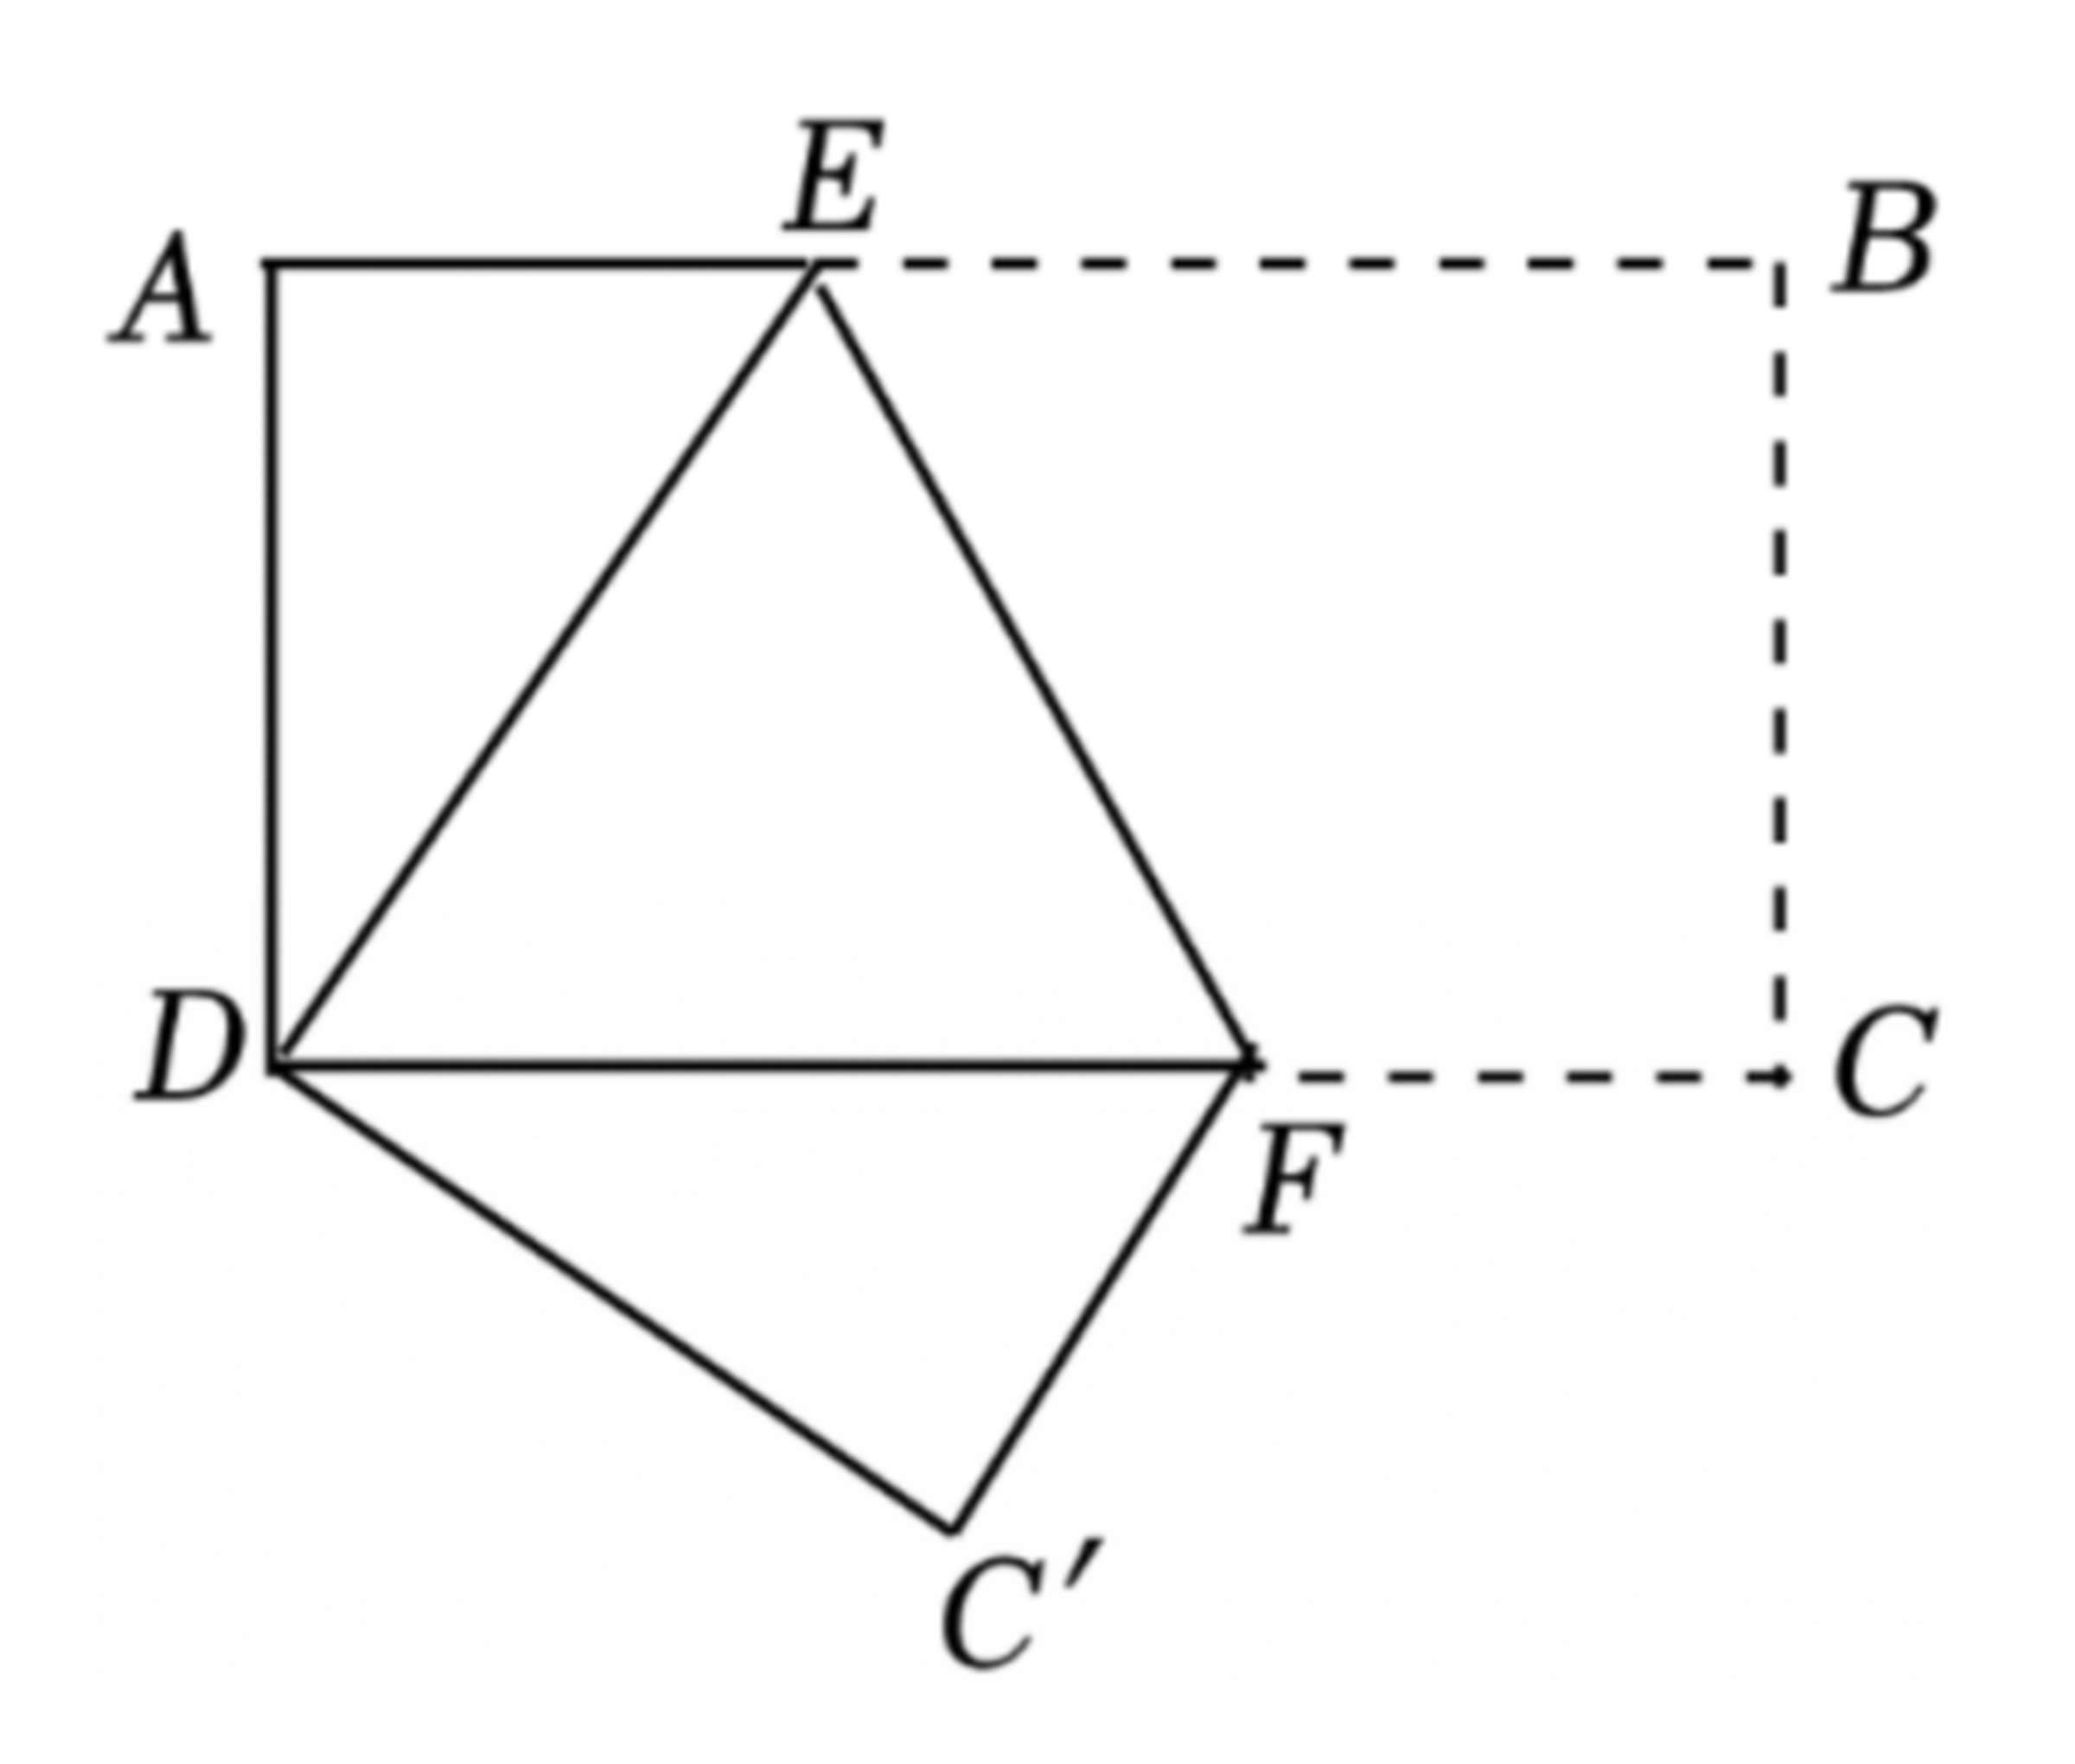
\includegraphics[width=0.40\textwidth]{figures/gao149_q11.png}
\end{center}

\ifanswer
\solbegin
\step{因为矩形 $ABCD(AB>AD)$ 的周长为 12，}
\step{在 $AB$ 和 $CD$ 边上分别取点 $E$ 和 $F$，将四边形 $BCFE$ 沿 $EF$ 折叠，}
\step{使点 $B$ 与点 $D$ 重合，此时点 $C$ 的对应点为 $C'$，}
\step{所以设 $AD=a$，$AB=b$，则 $2(a+b)=12$，}
\step{所以 $a+b=6$，且 $AB>AD$，所以 $b>a>0$，}
\step{设 $DF=x$，则 $C'F=b-x$，在 $Rt\triangle DC'F$ 中，$DC'=BC=a$，}% 几何三角形符号原卷印扁等边细线三角 $\triangle$，照录（放大 02 页确认）；$Rt$ 照录
\step{所以 $a^2+(b-x)^2=x^2$，解得 $x=\dfrac{a^2+b^2}{2b}$，}
\step{因此 $\triangle C'DF$ 的面积 $S=\dfrac{1}{2}\cdot DC'\cdot C'F=\dfrac{1}{2}\cdot a\cdot(b-x)$，}
\step{又 $b-x=b-\dfrac{(6-b)^2+b^2}{2b}=\dfrac{6(b-3)}{b}$，}
\step{所以 $S=\dfrac{1}{2}\cdot a\cdot\dfrac{6(b-3)}{b}=\dfrac{1}{2}\cdot(6-b)\cdot\dfrac{6(b-3)}{b}=\dfrac{3(6-b)(b-3)}{b}$}
\step{$=3\cdot\left(-b-\dfrac{18}{b}+9\right)$，又 $b+\dfrac{18}{b}\geqslant2\sqrt{b\cdot\dfrac{18}{b}}=6\sqrt{2}$，}
\step{当且仅当 $b=\dfrac{18}{b}$ 即 $b=3\sqrt{2}$ 时取等号，此时满足 $b>a$，}
\step{所以 $S\leqslant3\cdot(-6\sqrt{2}+9)=27-18\sqrt{2}$，故 $\triangle C'DF$ 面积的最大值为 $27-18\sqrt{2}$.}
\solend
\fi

% === Q12 === 解析内 3 幅三次函数曲线坐标图（仅答案版出）；解析 15 行（8 行 03 页＋7 行 04 页）
\item 已知 $m>0$，若存在 $t\in\R$，使得对任意 $x\in[0,m]$，不等式 $[(x-1)^2-t](x-t)\leqslant0$ 恒成立，则 $m$ 的最大值是\blankline[4.4em].

\ifanswer
\solbegin
\step{当 $t\leqslant0$ 时，$(x-1)^2-t\geqslant0$ 恒成立，}
\step{不等式 $[(x-1)^2-t](x-t)\leqslant0$ 的解集为 $x\leqslant t$，与 $x\in[0,m]$ 矛盾；}
\step{当 $t>0$ 时，不等式 $[(x-1)^2-t](x-t)\leqslant0\Leftrightarrow(x-1-\sqrt t)(x-1+\sqrt t)(x-t)\leqslant0$，}
\step{若 $t<1-\sqrt t$，即 $t\in\left(0,\dfrac{3-\sqrt5}{2}\right)$，}
\begin{center}
% 情形一 $t<1-\sqrt t$ 曲线图取 03 页右侧，去粉色水印、去色、4× LANCZOS 放大；仅答案版出
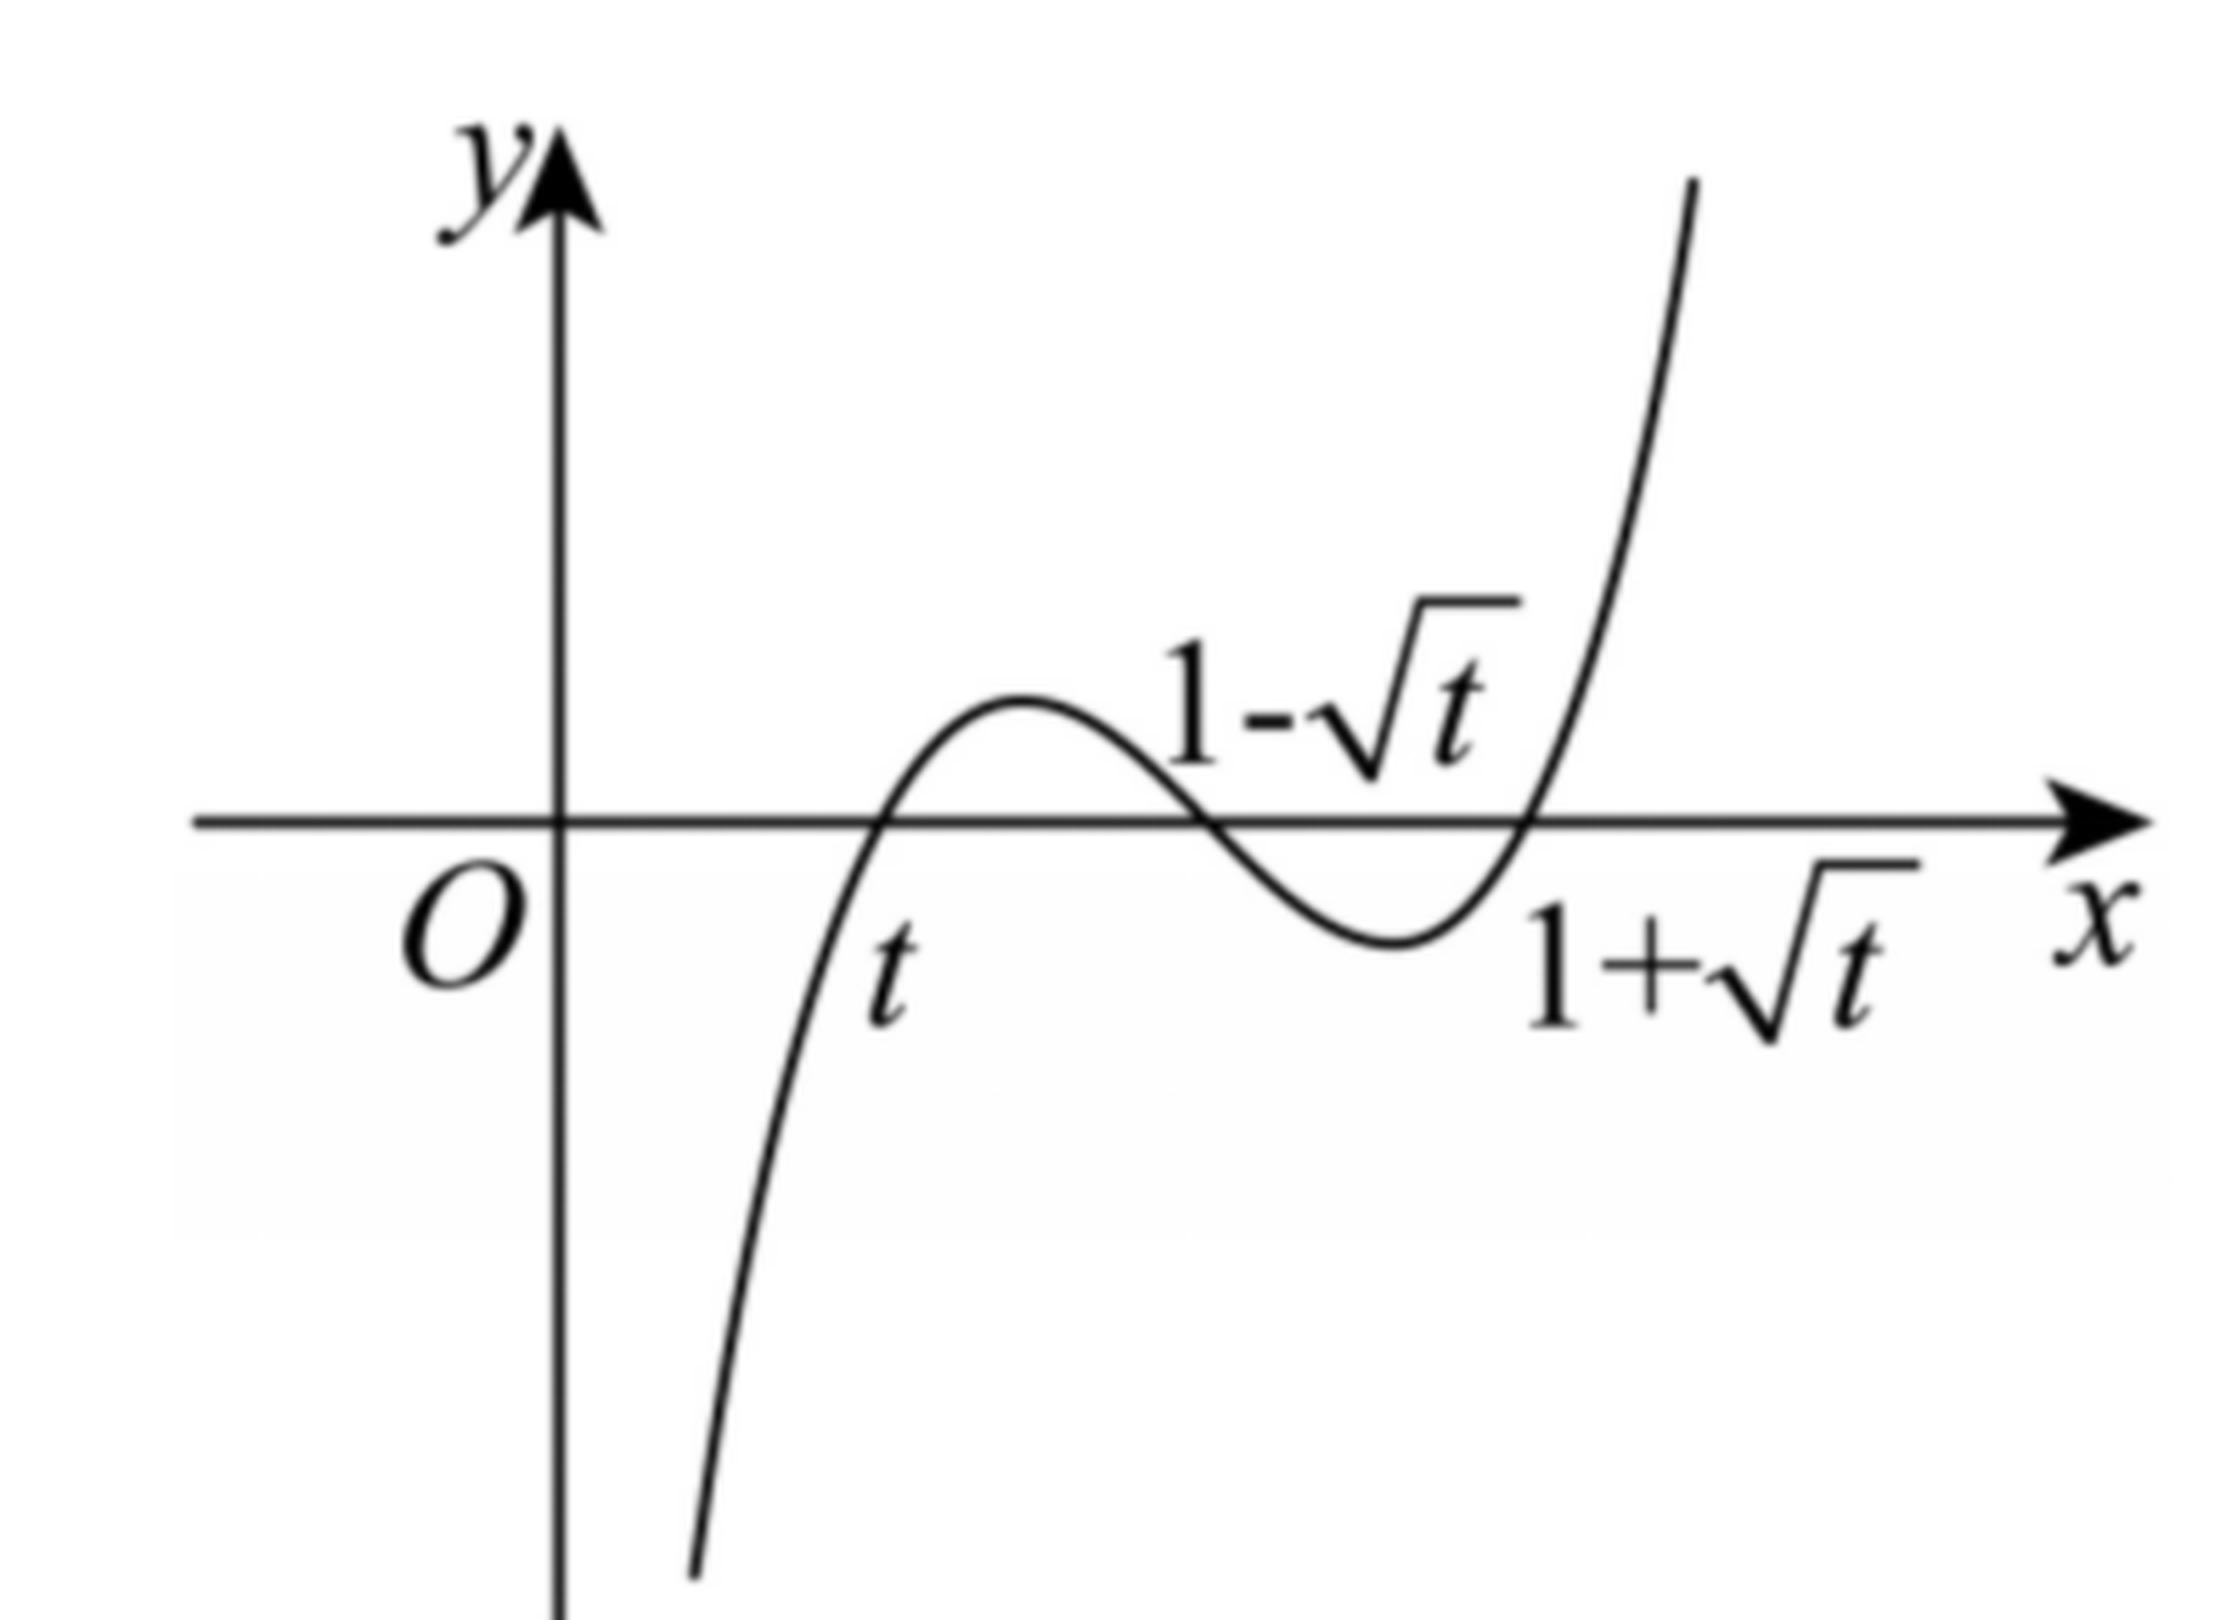
\includegraphics[width=0.40\textwidth]{figures/gao149_q12_a.png}
\end{center}
\step{则原不等式的解集为 $(-\infty,t]\cup[1-\sqrt t,1+\sqrt t]$，}
\step{当 $0<m\leqslant t$ 时，原不等式恒成立，因此}
\step{$m\in\left(0,\dfrac{3-\sqrt5}{2}\right)$；}
\step{若 $t=1-\sqrt t$，即 $t=\dfrac{3-\sqrt5}{2}$，则原不等式的解集为 $(-\infty,1+\sqrt t]$，}
\begin{center}
% 情形二 $t=1-\sqrt t$ 曲线图取 03 页右侧，去粉色水印、去色、4× LANCZOS 放大；仅答案版出
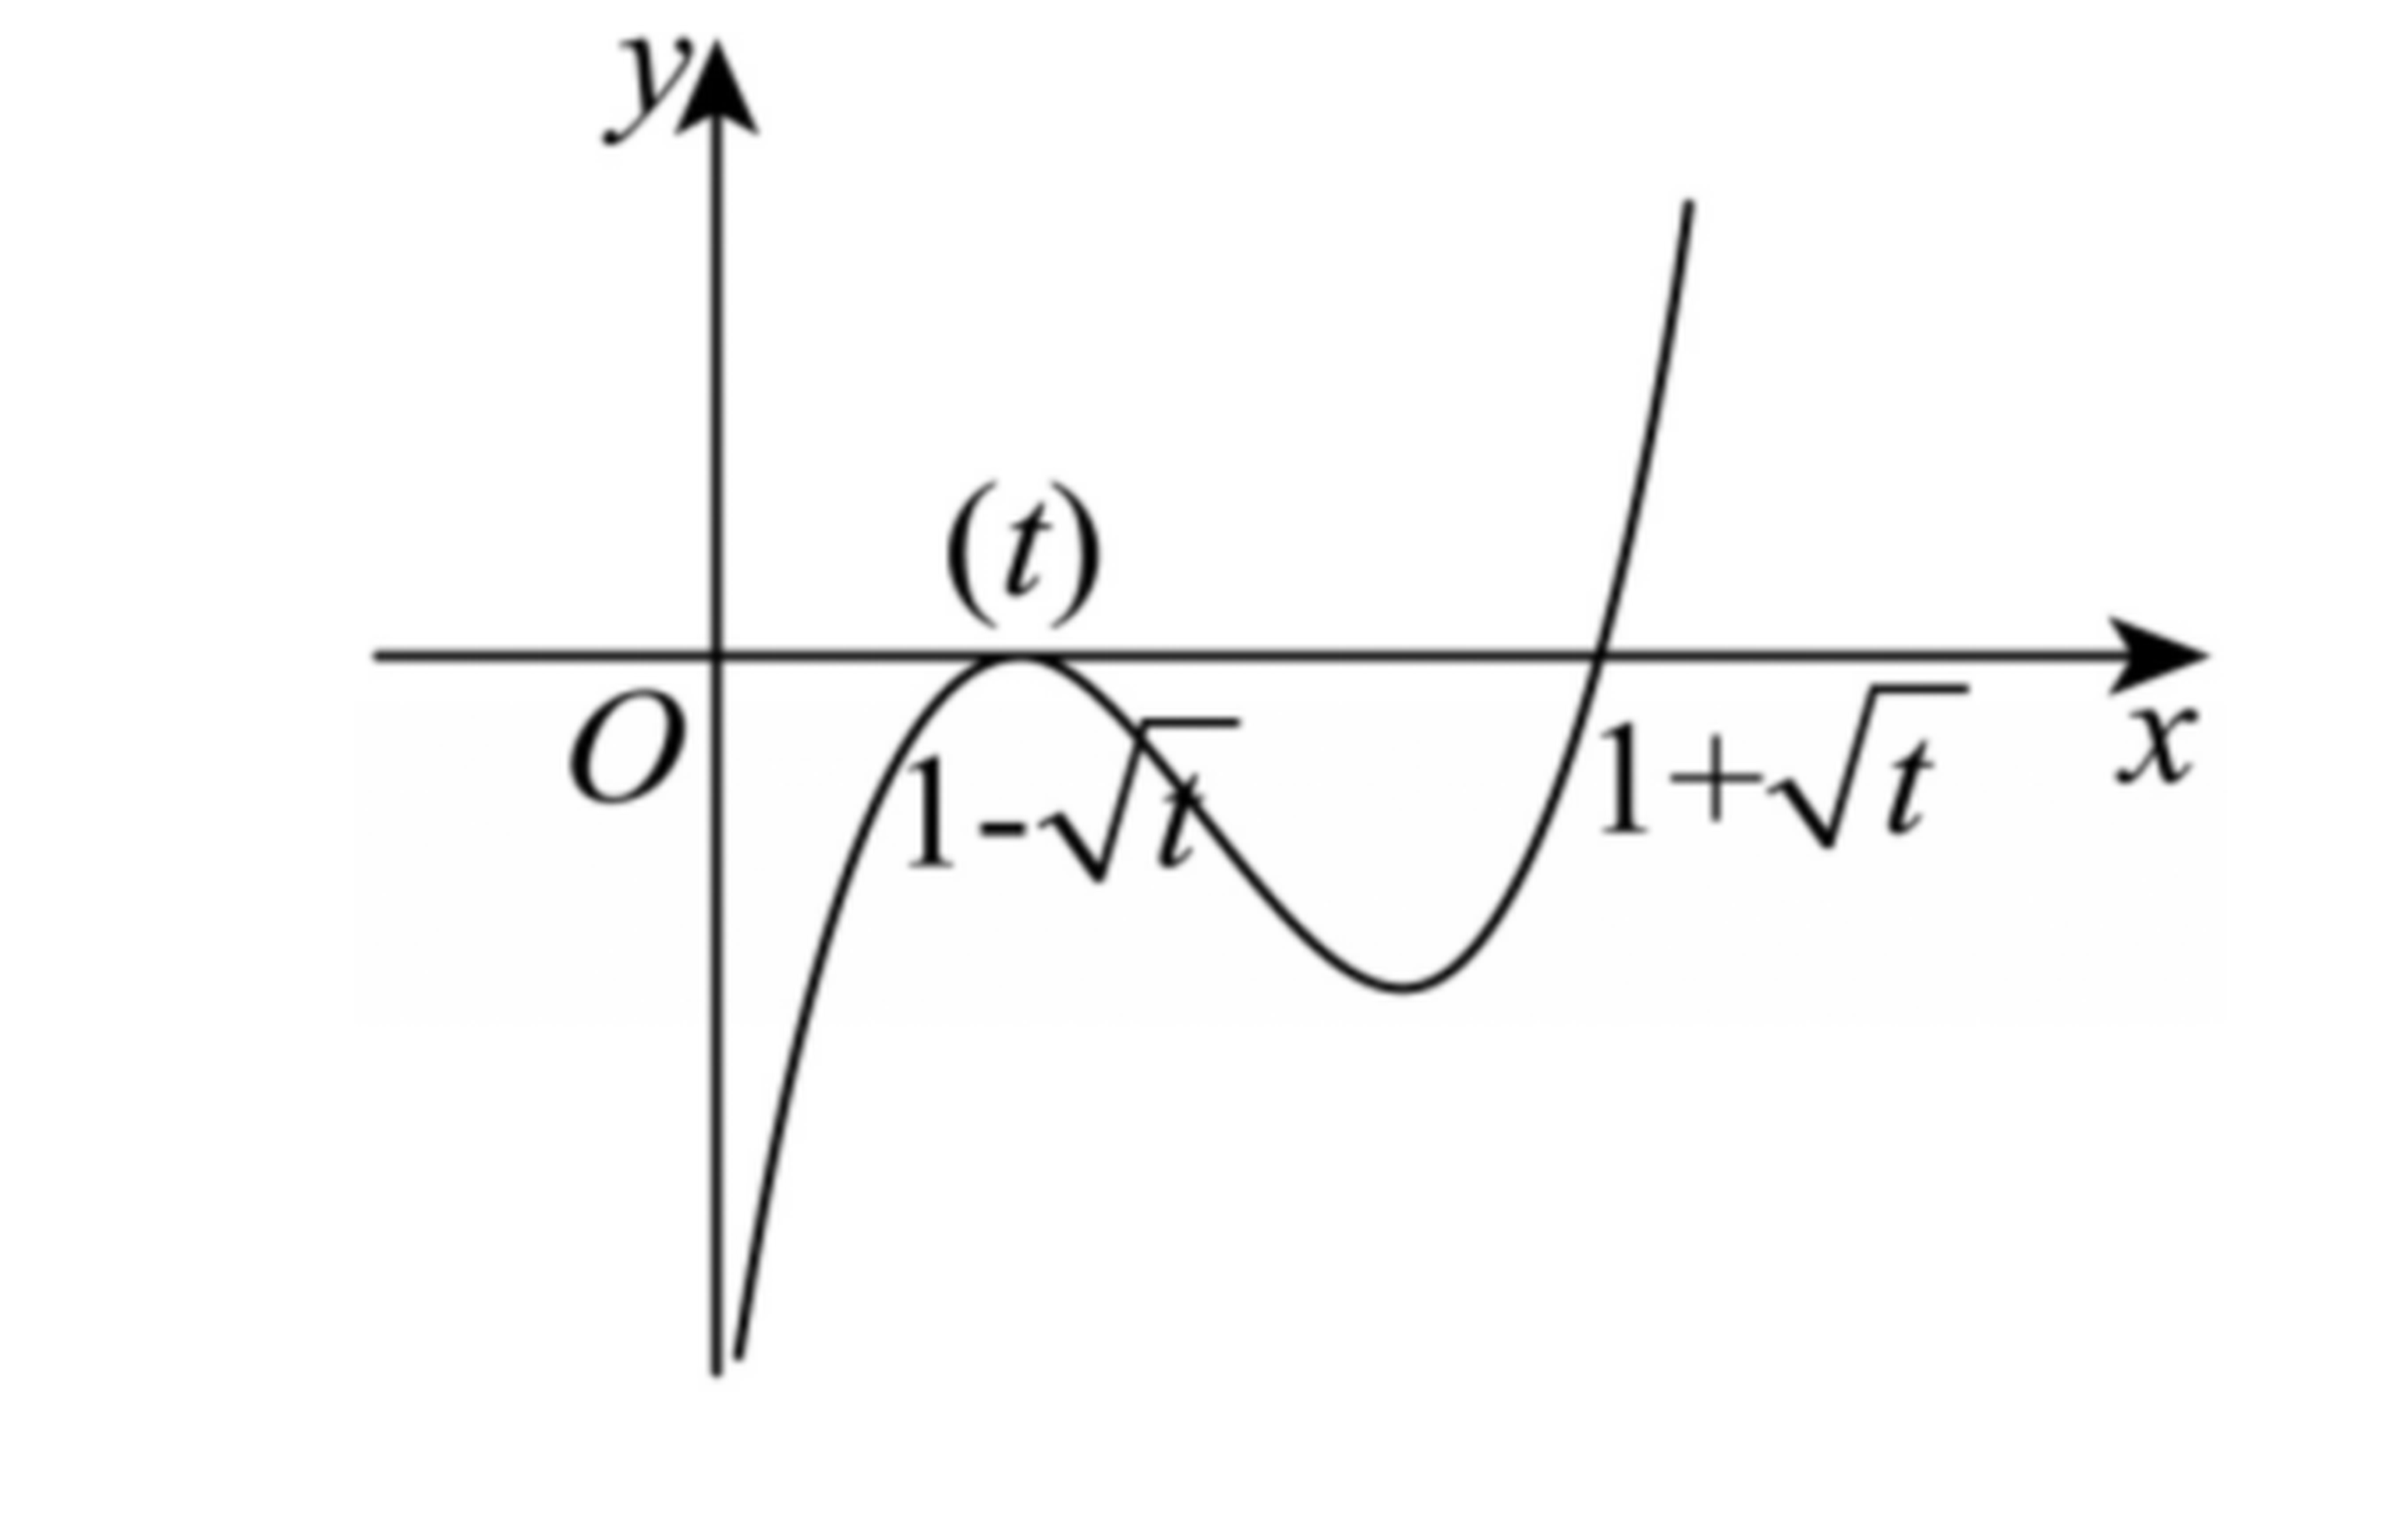
\includegraphics[width=0.40\textwidth]{figures/gao149_q12_b.png}
\end{center}
\step{当 $0<m\leqslant1+\sqrt t$ 时，原不等式恒成立，因此 $m\in\left(0,\dfrac{\sqrt5+1}{2}\right]$；}
\step{若 $1+\sqrt t>t>1-\sqrt t$，即 $t\in\left(\dfrac{3-\sqrt5}{2},\dfrac{3+\sqrt5}{2}\right)$，}
\begin{center}
% 情形三 $1+\sqrt t>t>1-\sqrt t$ 曲线图取 04 页右侧，去粉色水印、去色、4× LANCZOS 放大；仅答案版出
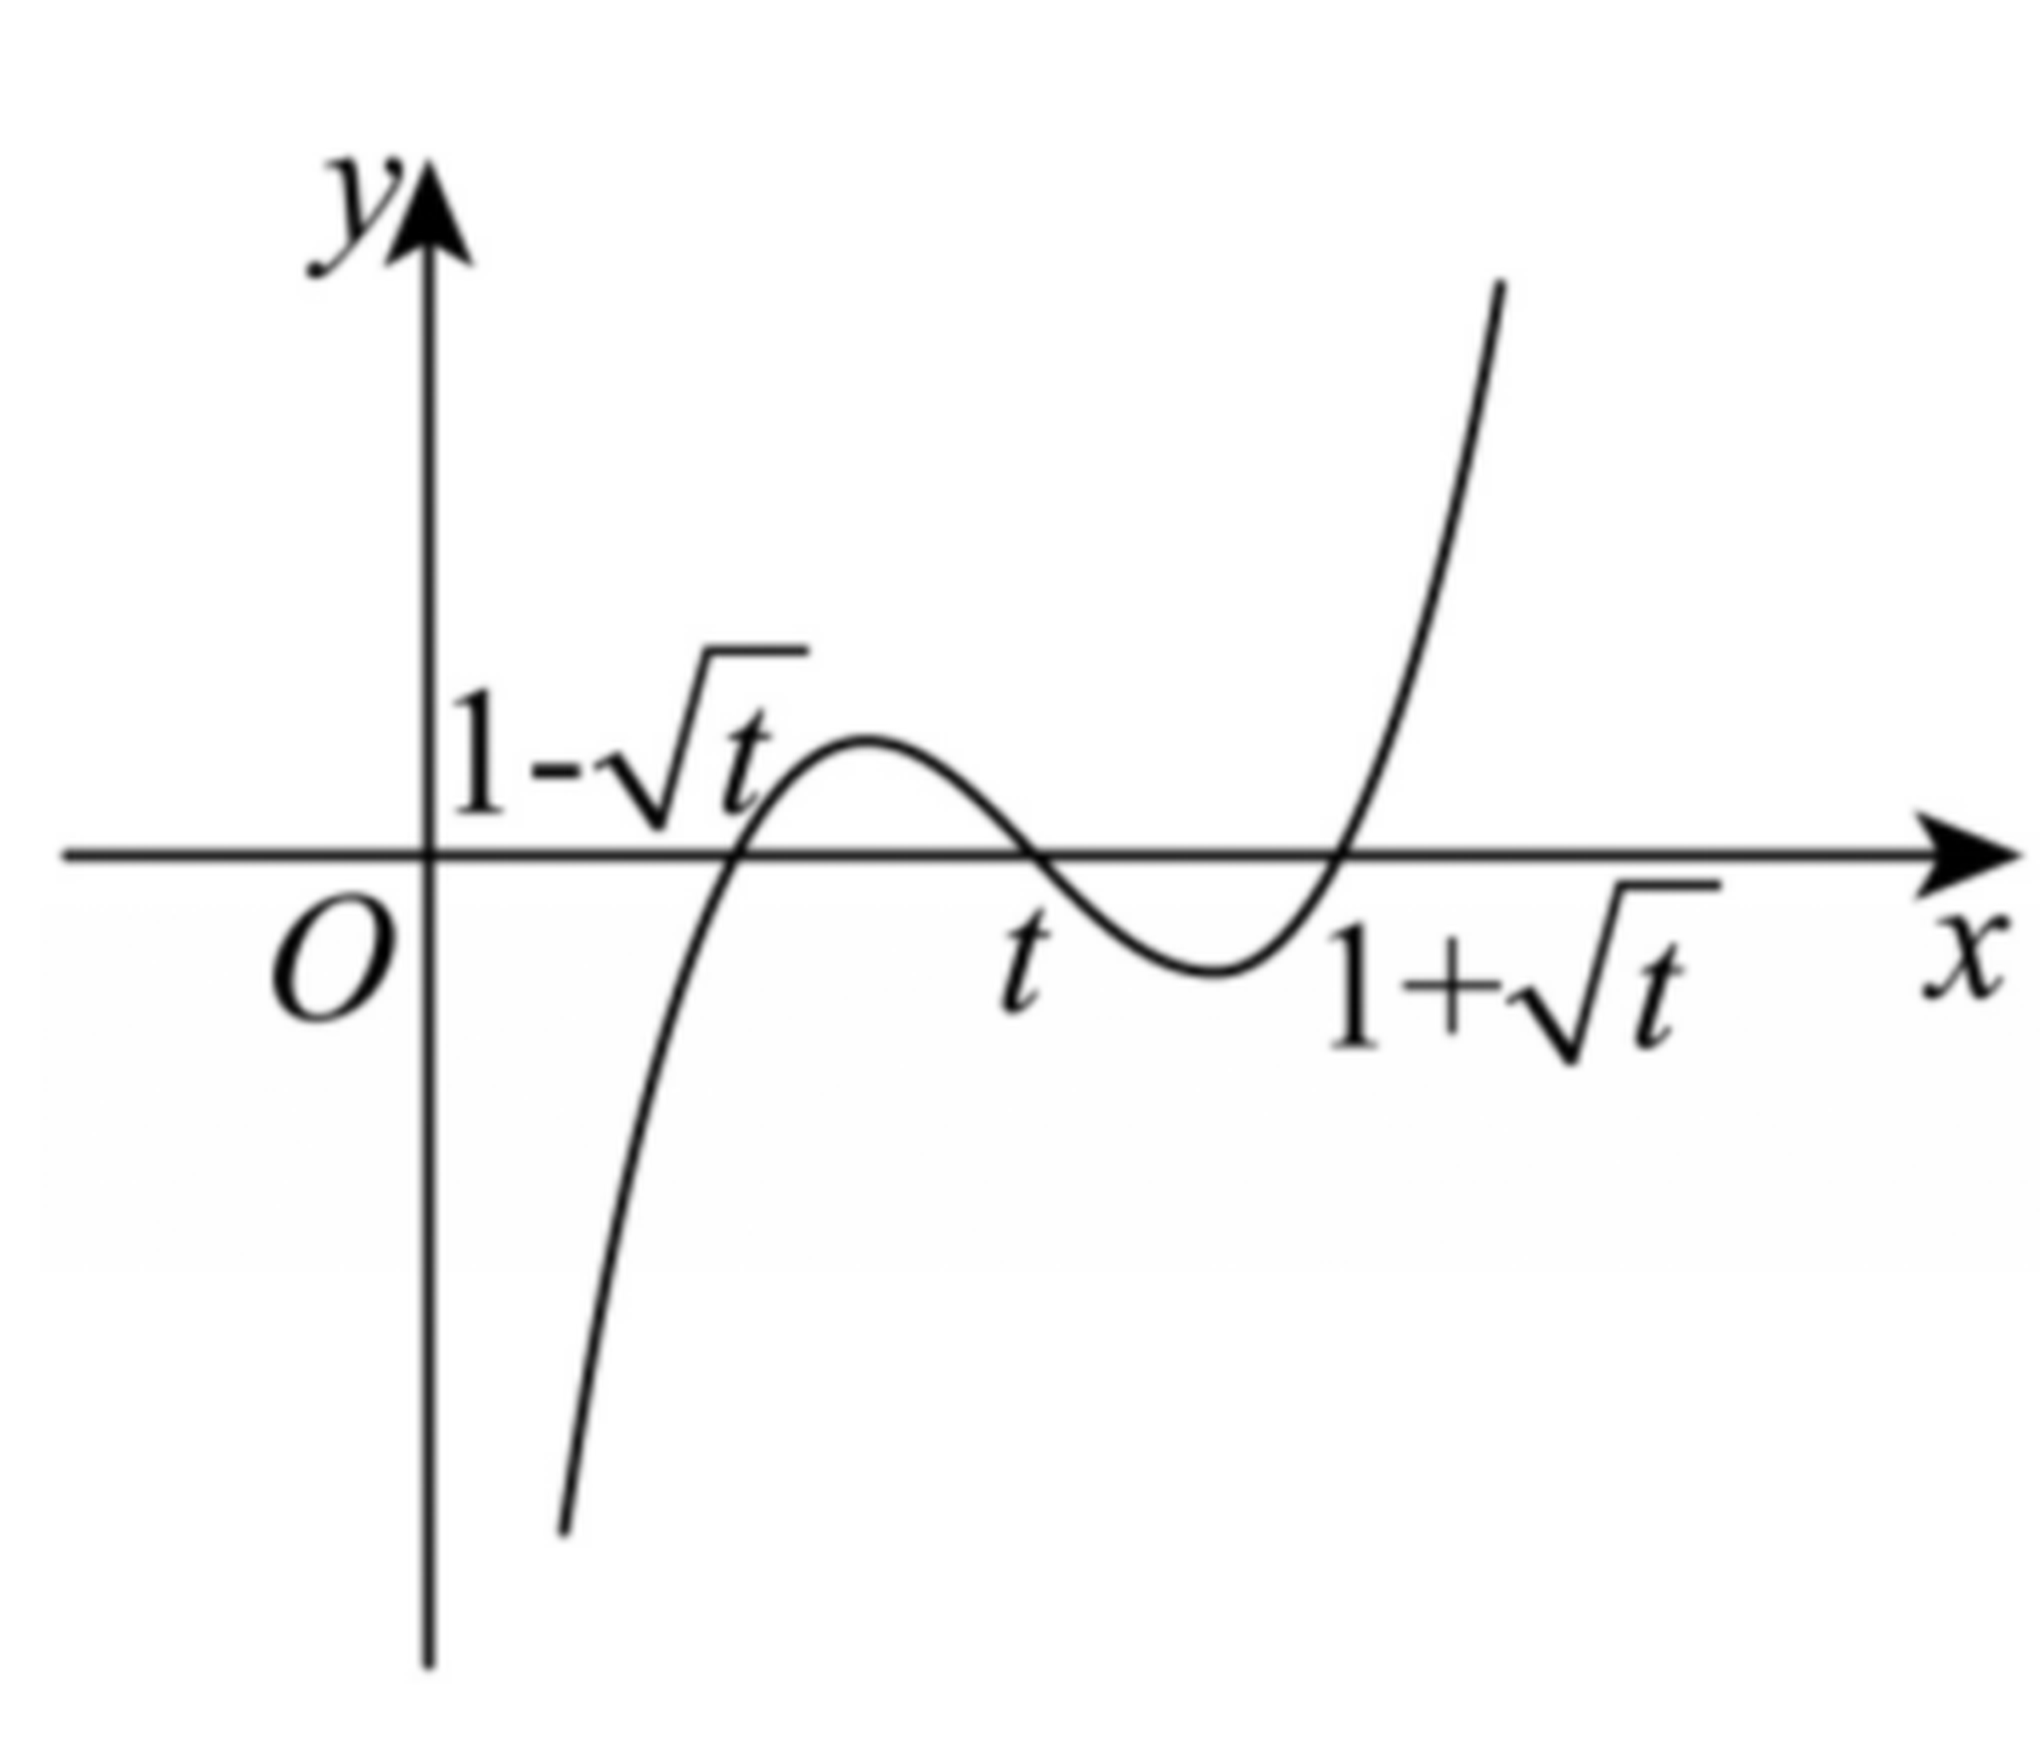
\includegraphics[width=0.40\textwidth]{figures/gao149_q12_c.png}
\end{center}
\step{则原不等式的解集为 $(-\infty,1-\sqrt t]\cup[t,1+\sqrt t]$，}
\step{当 $\begin{cases}1-\sqrt t>0\\1-\sqrt t\geqslant m\end{cases}$ 时，原不等式恒成立，此时 $t\in\left(\dfrac{3-\sqrt5}{2},1\right)$，$m\in\left(0,\dfrac{3-\sqrt5}{2}\right)$；}
\step{若 $t\geqslant1+\sqrt t$，即 $t\geqslant\dfrac{3+\sqrt5}{2}$，则取 $x=0$，$(t-1)t>0$，}
\step{原不等式不恒成立，不符合题意，}
\step{因此实数 $m$ 的取值范围是 $\left(0,\dfrac{\sqrt5+1}{2}\right]$，$m$ 的最大值是 $\dfrac{\sqrt5+1}{2}$.}
\solend
\fi

\end{enumerate}

\bigsec{二、选择题}

\begin{enumerate}
\setcounter{enumi}{12}

% === Q13 ===：答案"C"直接印在题干括号内、无【答案】/【解析】段，按 高一84 Q13／高一148 Q13 成例括号留空、另提 \ans{$C$}；四选项两行两列照原卷分行
\item 设 $ab>0$，则 $a>b$ 是 $\dfrac{1}{a}<\dfrac{1}{b}$ 的\mbox{（\quad）}

\keepwithprev
A. 充分不必要条件\qquad\qquad B. 必要不充分条件

C. 充要条件\qquad\qquad D. 既不充分又不必要条件

\ifanswer
\ans{$C$}
\fi

% === Q14 ===：$A\subset B$ 单线照录；四选项补集照原卷上划线 \overline{A}／\overline{B}；解析 1 行（由韦恩图得 B 对）
\item 已知集合 $A$、$B$ 非空，且 $A\subset B$，则下列式子中一定是空集的为\mbox{（\quad）}

\keepwithprev
A. $\overline{A}\cap B$\qquad B. $A\cap\overline{B}$\qquad C. $\overline{A}\cap\overline{B}$\qquad D. $\overline{A}\cup\overline{B}$

\ifanswer
\solbegin
\step{由韦恩图得 $B$ 对. 故选 $B$.}
\solend
\fi

% === Q15 ===："天文数字"弯引号照录；解析 2 行（首行在 04 页末、末行续 05 页顶）
\item 历史上数学计算方面的三大发明是阿拉伯数字、十进制和对数，其中对数的发明，大大缩短了计算时间，为人类研究科学和了解自然起了重大作用，对数运算对估算“天文数字”具有独特的优势. $2.5^{1000}$ 的估算值约为\mbox{（\quad）}

\keepwithprev
A. $10^{365}$\qquad B. $10^{379}$\qquad C. $10^{389}$\qquad D. $10^{398}$

\ifanswer
\solbegin
\step{$\lg 2.5^{1000}=1000\lg 2.5=1000(1-2\lg 2)\approx1000\times(1-0.602)=398$，}
\step{所以 $2.5^{1000}\approx10^{398}$. 故选 $D$.}
\solend
\fi

% === Q16 ===："完美集"新定义、圈数字①②文本模式；题干"若对任意 $x$，$y\in A$"用全角逗号、解析用顿号"$x$、$y\in A$"，两处照录不统一；解析 9 行
\item 设全集 $U=\R$，集合 $A$ 是一个非空数集，若对任意 $x$，$y\in A$，都有 $x+y\in A$、$xy\in A$，则称集合 $A$ 为一个“完美集”，给出以下命题：

①若 $A_1$、$A_2$ 都是“完美集”，且 $A_1\cap A_2\ne\varnothing$，则 $A_1\cap A_2$ 也是“完美集”；

②若 $A_1$、$A_2$ 都是“完美集”，则 $A_1\cup A_2$ 也是“完美集”.

下列说法正确的是\mbox{（\quad）}

\keepwithprev
A. ①②都是真命题\qquad\qquad B. ①是真命题，②是假命题

C. ①是假命题，②是真命题\qquad\qquad D. ①②都是假命题

\ifanswer
\solbegin
\step{由题意，全集 $U=\R$，集合 $A$ 是一个非空数集，}
\step{若对任意 $x$、$y\in A$，都有 $x+y\in A$、$xy\in A$，则称集合 $A$ 为一个“完美集”，}
\step{对于①，取 $x$、$y\in A_1\cap A_2$，则 $x\in A_1$，$x\in A_2$，$y\in A_1$，$y\in A_2$，}
\step{又 $A_1$、$A_2$ 是“完美集”，所以 $x+y\in A_1$，$xy\in A_1$，$x+y\in A_2$，$xy\in A_2$，}
\step{所以 $x+y\in A_1\cap A_2$，$xy\in A_1\cap A_2$，所以 $A_1\cap A_2$ 是“完美集”，故①正确；}
\step{对于②，取“完美集” $A_1=\{x\mid x=2k,k\in\Z\}$，$A_2=\{x\mid x=3k,k\in\Z\}$，}
\step{则 $2\in A_1$，$3\in A_2$，但 $2+3\notin A_1\cup A_2$，}
\step{即此时 $A_1\cup A_2$ 不是“完美集”，故②错误.}
\step{故选 $B$.}
\solend
\fi
\end{enumerate}

\bigsec{三、解答题}

\begin{enumerate}
\setcounter{enumi}{16}

% === Q17 ===："图像"（有亻）照录（Q17 题干与解析共 2 处）；绝对值 \lvert…\rvert；解析 7 行
\item 已知 $m\in\R$，$f(x)=(m^2-m-5)x^m$. 若 $y=f(x)$ 是幂函数，且其图像不经过原点.

(1) 求实数 $m$ 的值；

(2) 若 $f(a)=f(b)$ 且 $a\ne b$，求 $\lvert a+2\rvert+\lvert b-1\rvert$ 的最小值，并指出取到最小值时 $a$ 的取值范围.

\ifanswer
\solbegin
\step{(1) $f(x)=(m^2-m-5)x^m$ 是幂函数，得 $m^2-m-5=1$，即 $m^2-m-6=0$，}
\step{解得 $m=-2$ 或 $m=3$，又函数图像不经过原点，所以 $m=-2$($3$ 舍)；}
\step{(2) 由 (1) 得 $f(x)=x^{-2}=\dfrac{1}{x^2}$ 为偶函数，}
\step{$x<0$ 时，函数 $f(x)$ 严格增，$x>0$ 时，函数 $f(x)$ 严格减，}
\step{又 $f(a)=f(b)$ 且 $a\ne b$，所以 $a=-b$，且 $a\ne0$，$b\ne0$，}
\step{则 $\lvert a+2\rvert+\lvert b-1\rvert=\lvert a+2\rvert+\lvert-a-1\rvert=\lvert a+2\rvert+\lvert a+1\rvert$，}
\step{则 $\lvert a+2\rvert+\lvert b-1\rvert$ 的最小值为 $1$，取到最小值时 $a$ 的取值范围是 $[-2,-1]$.}
\solend
\fi

% === Q18 ===：判别式两形混用——(1) cases 块印高 \Delta、(2) 独立行印扁 \triangle，逐处照录不统一；解析 8 行
\item 已知命题 $p$：方程 $x^2+4x+m-1=0$ 有两个不等的负根；命题 $q$：方程 $4x^2+4x+m-2=0$ 无实根.

(1) 若 $p$ 为真命题，求 $m$ 的取值范围；

(2) 若 $p$、$q$ 两命题一真一假，求 $m$ 的取值范围.

\ifanswer
\solbegin
\step{(1) 若 $p$ 为真命题，即方程 $x^2+4x+m-1=0$ 有两个不等的负根；}
\step{必有 $\begin{cases}\Delta=16-4(m-1)>0\\m-1>0\end{cases}$，解得 $1<m<5$，即 $m$ 的取值范围为 $(1,5)$；}
\step{(2) 命题 $q$：方程 $4x^2+4x+m-2=0$ 无实根，}
\step{则有 $\triangle=16-16(m-2)<0$，解得 $m>3$，}
\step{若 $p$ 和 $q$ 有且只有一个为真命题，}
\step{若 $p$ 真 $q$ 假，必有 $\begin{cases}1<m<5\\m\leqslant3\end{cases}$，则有 $1<m\leqslant3$，}
\step{若 $p$ 假 $q$ 真，必有 $\begin{cases}m\leqslant1\text{ 或 }m\geqslant5\\m>3\end{cases}$，则有 $m\geqslant5$，}
\step{综上，$1<m\leqslant3$ 或 $m\geqslant5$.}
\solend
\fi

% === Q19 ===：$A\subseteq B$ 带下划线照录；解析 7 行（(2) 两组 cases 并排）
\item 已知 $m\in\R$，集合 $A=\left\{x\mid y=\sqrt{3-x}-\dfrac{1}{\sqrt{x-1}}\right\}$，集合 $B=\{x\mid 2m\leqslant x\leqslant1-m\}$.

(1) 若 $A\cup B=B$，求实数 $m$ 的取值范围；

(2) 若 $A\cap B=\varnothing$，求实数 $m$ 的取值范围.

\ifanswer
\solbegin
\step{(1) 函数 $y=\sqrt{3-x}-\dfrac{1}{\sqrt{x-1}}$，则 $\begin{cases}3-x\geqslant0\\x-1>0\end{cases}$，解得 $1<x\leqslant3$，}
\step{所以 $A=\{x\mid1<x\leqslant3\}$，}
\step{因为 $A\cup B=B$，所以 $A\subseteq B$，则 $\begin{cases}2m\leqslant1\\1-m\geqslant3\end{cases}$，解得 $m\leqslant-2$，}
\step{综上，实数 $m$ 的取值范围为 $(-\infty,-2]$；}
\step{(2) 当 $B=\varnothing$ 时，则 $2m>1-m$，解得 $m>\dfrac{1}{3}$，}
\step{当 $B\ne\varnothing$ 时，则 $\begin{cases}2m\leqslant1-m\\2m>3\end{cases}$ 或 $\begin{cases}2m\leqslant1-m\\1-m\leqslant1\end{cases}$，解得 $m\in\varnothing$ 或 $0\leqslant m\leqslant\dfrac{1}{3}$，}
\step{综上，实数 $m$ 的取值范围为 $[0,+\infty)$.}
\solend
\fi

% === Q20 ===：n 阶基本不等式推广；(3) 解析含 \overbrace{…}^{k} 上括号；(2) 解析"x=x=x=3(1-x)"三连等系原卷笔误、照录加注（见 ⑤）；解析 14 行
\item 教材中的基本不等式可以推广到 $n$ 阶：$n$ 个正数的算术平均数不小于它们的几何平均数，即对于任意的正数 $a_1$、$a_2$、$\cdots$、$a_n$，有 $\dfrac{a_1+a_2+\cdots+a_n}{n}\geqslant\sqrt[n]{a_1\cdot a_2\cdots a_n}$（$n\in\N$ 且 $n\geqslant2$），且等号当且仅当 $a_1=a_2=\cdots=a_n$ 时成立. 利用此结论解决下列问题：

(1) 若 $x$、$y$、$z>0$，求 $\dfrac{y}{x}+\dfrac{2z}{y}+\dfrac{4x}{z}$ 的最小值；

(2) 已知 $0<x<1$，求 $x^3(1-x)$ 的最大值，并求取得最大值时的 $x$ 的值；

(3) 对任意的正整数 $k$，判断 $\left(1+\dfrac{1}{k}\right)^k$ 与 $\left(1+\dfrac{1}{k+1}\right)^{k+1}$ 的大小关系，并证明.

\ifanswer
\solbegin
\step{(1) 因为 $x$、$y$、$z>0$，有 $\dfrac{y}{x}>0$，$\dfrac{2z}{y}>0$，$\dfrac{4x}{z}>0$}
\step{所以 $\dfrac{y}{x}+\dfrac{2z}{y}+\dfrac{4x}{z}\geqslant3\sqrt[3]{\dfrac{y}{x}\cdot\dfrac{2z}{y}\cdot\dfrac{4x}{z}}=3\sqrt[3]{8}=6$，}
\step{当且仅当 $\dfrac{y}{x}=\dfrac{2z}{y}=\dfrac{4x}{z}$ 时取等号，故 $\dfrac{y}{x}+\dfrac{2z}{y}+\dfrac{4x}{z}$ 的最小值为 $6$.}
\step{(2) 因为 $0<x<1$，所以 $1-x>0$，}
\step{$x^3(1-x)=\dfrac{1}{3}[x\cdot x\cdot x\cdot3(1-x)]\leqslant\dfrac{1}{3}\left[\dfrac{x+x+x+3(1-x)}{4}\right]^4=\dfrac{1}{3}\times\left(\dfrac{3}{4}\right)^4$}
\step{$=\dfrac{27}{256}$，当且仅当 $x=x=x=3(1-x)$，即 $x=3(1-x)$，$x=\dfrac{3}{4}$ 取等号，}% 原卷"x=x=x=3(1-x)"三连等，疑为四因子相等之误排，放大 08 页确认，照录未改（见 ⑤）
\step{所以 $0<x<1$ 时，$x^3(1-x)$ 的最大值是 $\dfrac{27}{256}$，取最大值时 $x=\dfrac{3}{4}$.}
\step{(3) 对任意 $k\in\N^*$，$\left(1+\dfrac{1}{k}\right)^k<\left(1+\dfrac{1}{k+1}\right)^{k+1}$.}
\step{证明：$\left(1+\dfrac{1}{k}\right)^k=\overbrace{\left(1+\dfrac{1}{k}\right)\cdot\left(1+\dfrac{1}{k}\right)\cdots\left(1+\dfrac{1}{k}\right)}^{k}\times1$}
\step{$\leqslant\left(\dfrac{\overbrace{\left(1+\dfrac{1}{k}\right)+\left(1+\dfrac{1}{k}\right)+\cdots+\left(1+\dfrac{1}{k}\right)}^{k}+1}{k+1}\right)^{k+1}$}
\step{$=\left(\dfrac{\overbrace{(1+1+\cdots+1)}^{k}+\overbrace{\left(\dfrac{1}{k}+\dfrac{1}{k}+\cdots+\dfrac{1}{k}\right)}^{k}+1}{k+1}\right)^{k+1}=\left(\dfrac{k+1+1}{k+1}\right)^{k+1}=\left(1+\dfrac{1}{k+1}\right)^{k+1}$，}
\step{当且仅当 $1+\dfrac{1}{k}=1$ 时取等号，}
\step{但是任意 $k\in\N^*$ 时 $1+\dfrac{1}{k}>1$，所以等号不成立，}
\step{故任意 $k\in\N^*$ 时，$\left(1+\dfrac{1}{k}\right)^k<\left(1+\dfrac{1}{k+1}\right)^{k+1}$.}
\solend
\fi

% === Q21 ===："减 k 集"新定义（引号内 k／数字两侧空格照录）；解析 26 行（续 10 页），含 ⑤ 三处原卷笔误照录
\item 定义：对于给定的整数 $k$，若非空集合 $A$ 满足如下 3 个条件：

① $A$ 是正整数集的子集；② $A\ne\{1\}$；

③对任意正整数 $x,y$，若 $x+y\in A$，则 $xy-k\in A$；则称集合 $A$ 为“减 $k$ 集”.

(1) 判断集合 $A=\{1,2\}$ 是否为“减 $0$ 集”？是否为“减 $1$ 集”？（无需说明理由）

(2) 证明：不存在“减 $2$ 集”；

(3) 是否存在“减 $1$ 集”？如果存在，求出所有“减 $1$ 集”；如果不存在，说明理由.

\ifanswer
\solbegin
\step{(1) 因为 $P\subseteq\N^*$，$P\ne\{1\}$，$1+1=2\in P$，$1\times1-0\in P$，}
\step{所以集合 $P=\{1,2\}$ 是“减 $0$ 集”；}
\step{因为 $P\subseteq\N^*$，$P\ne\{1\}$，$1+1=2\in P$，$1\times1-1\notin P$，}
\step{所以集合 $P=\{1,2\}$ 是“减 $1$ 集”；}% 按条件③应为"不是"，原卷径印"是"，放大 09 页确认，照录未改（见 ⑤）
\step{(2) 假设存在集合 $A$ 是“减 $2$ 集”，若 $x+y\in A$，则 $xy-2\in A$，}
\step{①当 $x+y=xy-2$ 时，有 $(x-1)(y-1)=3$，}
\step{则 $x$、$y$ 一个为 $2$，一个为 $4$，所以集合 $A$ 有元素 $6$，}
\step{但 $3+3\in A$，$3\times3-2\notin A$，与 $A$ 是“减 $2$ 集”矛盾；}
\step{②当 $x+y\ne xy-2$ 时，则 $x+y=xy-1$ 或 $x+y=xy-m$($m>2$)，}
\step{若 $x+y=xy-1$，$m=1$ 时，$M$ 为除 $1$ 以外的最小元素，}% 原卷"m=1"上文未显式定义，疑笔误，放大 09 页确认，照录未改（见 ⑤）
\step{则 $x=M-1$，$y=1$ 时，$xy-2=M-3$ 小于 $M$，}
\step{要符合题意，必须 $M=4$，}
\step{此时取 $x-2$，$y=2$，$xy-2=2$ 不属于 $A$，故不符合题意，}% 原卷"取 x−2"疑为"取 x=2"误排，放大 09 页确认，照录未改（见 ⑤）
\step{当 $m>2$ 时，$(x-1)(y-1)=m+1$，同样得出矛盾，}
\step{综上，不存在 $A$ 是“减 $2$ 集”.}
\step{(3) 存在“减 $1$ 集” $A$，则 $A\ne\{1\}$，}
\step{①假设 $1\in A$，则 $A$ 中除了元素 $1$ 以外，必然还含有其它元素，}
\step{假设 $2\in A$，$1+1\in A$，而 $1\times1-1\notin A$，所以 $2\notin A$，}
\step{假设 $3\in A$，$1+2\in A$，而 $1\times2-1\in A$，所以 $3\in A$，}
\step{所以 $A=\{1,3\}$，}
\step{假设 $4\in A$，$1+3\in A$，而 $1\times3-1\notin A$，所以 $4\notin A$，}
\step{假设 $5\in A$，$1+4\in A$，$1\times4-1\in A$，$2+3=5$，$2\times3-1\in A$，所以 $5\in A$，}
\step{所以 $A=\{1,3,5\}$，}
\step{以此类推，得 $A=\{1,3,5,\cdots,2n-1,\cdots\}$，($n\in\N^*$)，}
\step{所以所有的“减 $1$ 集”有 $\{1,3\}$，$\{1,3,5\}$，$\{1,3,5,7\}$，$\cdots$，$\{1,3,5,\cdots,2n-1,\cdots\}$，}
\step{$(n\in\N^*)$.}
\solend
\fi
\end{enumerate}

\end{document}
